\documentclass[twoside]{book}

% Packages required by doxygen
\usepackage{fixltx2e}
\usepackage{calc}
\usepackage{doxygen}
\usepackage[export]{adjustbox} % also loads graphicx
\usepackage{graphicx}
\usepackage[utf8]{inputenc}
\usepackage{makeidx}
\usepackage{multicol}
\usepackage{multirow}
\PassOptionsToPackage{warn}{textcomp}
\usepackage{textcomp}
\usepackage[nointegrals]{wasysym}
\usepackage[table]{xcolor}

% Font selection
\usepackage[T1]{fontenc}
\usepackage[scaled=.90]{helvet}
\usepackage{courier}
\usepackage{amssymb}
\usepackage{sectsty}
\renewcommand{\familydefault}{\sfdefault}
\allsectionsfont{%
  \fontseries{bc}\selectfont%
  \color{darkgray}%
}
\renewcommand{\DoxyLabelFont}{%
  \fontseries{bc}\selectfont%
  \color{darkgray}%
}
\newcommand{\+}{\discretionary{\mbox{\scriptsize$\hookleftarrow$}}{}{}}

% Page & text layout
\usepackage{geometry}
\geometry{%
  a4paper,%
  top=2.5cm,%
  bottom=2.5cm,%
  left=2.5cm,%
  right=2.5cm%
}
\tolerance=750
\hfuzz=15pt
\hbadness=750
\setlength{\emergencystretch}{15pt}
\setlength{\parindent}{0cm}
\setlength{\parskip}{3ex plus 2ex minus 2ex}
\makeatletter
\renewcommand{\paragraph}{%
  \@startsection{paragraph}{4}{0ex}{-1.0ex}{1.0ex}{%
    \normalfont\normalsize\bfseries\SS@parafont%
  }%
}
\renewcommand{\subparagraph}{%
  \@startsection{subparagraph}{5}{0ex}{-1.0ex}{1.0ex}{%
    \normalfont\normalsize\bfseries\SS@subparafont%
  }%
}
\makeatother

% Headers & footers
\usepackage{fancyhdr}
\pagestyle{fancyplain}
\fancyhead[LE]{\fancyplain{}{\bfseries\thepage}}
\fancyhead[CE]{\fancyplain{}{}}
\fancyhead[RE]{\fancyplain{}{\bfseries\leftmark}}
\fancyhead[LO]{\fancyplain{}{\bfseries\rightmark}}
\fancyhead[CO]{\fancyplain{}{}}
\fancyhead[RO]{\fancyplain{}{\bfseries\thepage}}
\fancyfoot[LE]{\fancyplain{}{}}
\fancyfoot[CE]{\fancyplain{}{}}
\fancyfoot[RE]{\fancyplain{}{\bfseries\scriptsize Generated by Doxygen }}
\fancyfoot[LO]{\fancyplain{}{\bfseries\scriptsize Generated by Doxygen }}
\fancyfoot[CO]{\fancyplain{}{}}
\fancyfoot[RO]{\fancyplain{}{}}
\renewcommand{\footrulewidth}{0.4pt}
\renewcommand{\chaptermark}[1]{%
  \markboth{#1}{}%
}
\renewcommand{\sectionmark}[1]{%
  \markright{\thesection\ #1}%
}

% Indices & bibliography
\usepackage{natbib}
\usepackage[titles]{tocloft}
\setcounter{tocdepth}{3}
\setcounter{secnumdepth}{5}
\makeindex

% Hyperlinks (required, but should be loaded last)
\usepackage{ifpdf}
\ifpdf
  \usepackage[pdftex,pagebackref=true]{hyperref}
\else
  \usepackage[ps2pdf,pagebackref=true]{hyperref}
\fi
\hypersetup{%
  colorlinks=true,%
  linkcolor=blue,%
  citecolor=blue,%
  unicode%
}

% Custom commands
\newcommand{\clearemptydoublepage}{%
  \newpage{\pagestyle{empty}\cleardoublepage}%
}

\usepackage{caption}
\captionsetup{labelsep=space,justification=centering,font={bf},singlelinecheck=off,skip=4pt,position=top}

%===== C O N T E N T S =====

\begin{document}

% Titlepage & ToC
\hypersetup{pageanchor=false,
             bookmarksnumbered=true,
             pdfencoding=unicode
            }
\pagenumbering{alph}
\begin{titlepage}
\vspace*{7cm}
\begin{center}%
{\Large V\+I\+NS M\+O\+NO C\+O\+M\+M\+E\+N\+T\+ED \\[1ex]\large 1.\+0.\+0 }\\
\vspace*{1cm}
{\large Generated by Doxygen 1.8.13}\\
\end{center}
\end{titlepage}
\clearemptydoublepage
\pagenumbering{roman}
\tableofcontents
\clearemptydoublepage
\pagenumbering{arabic}
\hypersetup{pageanchor=true}

%--- Begin generated contents ---
\chapter{D\+Bo\+W2 Library}
\label{index}\hypertarget{index}{}\hyperlink{namespaceDBoW2}{D\+Bo\+W2} library for C++\+: Bag-\/of-\/word image database for image retrieval.

Written by Dorian Galvez-\/\+Lopez, University of Zaragoza

Check my website to obtain updates\+: \href{http://doriangalvez.com}{\tt http\+://doriangalvez.\+com}\hypertarget{index_requirements}{}\section{Requirements}\label{index_requirements}
This library requires the \hyperlink{namespaceDUtils}{D\+Utils}, D\+Utils\+CV, \hyperlink{namespaceDVision}{D\+Vision} and Open\+CV libraries, as well as the boost\+::dynamic\+\_\+bitset class.\hypertarget{index_citation}{}\section{Citation}\label{index_citation}
If you use this software in academic works, please cite\+: 
\begin{DoxyPre}
  @ARTICLE\{GalvezTRO12,
   author=\{Galvez-Lopez, Dorian and Tardos, J. D.\}, 
   journal=\{IEEE Transactions on Robotics\},
   title=\{Bags of Binary Words for Fast Place Recognition in Image Sequences\},
   year=\{2012\},
   month=\{October\},
   volume=\{28\},
   number=\{5\},
   pages=\{1188--1197\},
   doi=\{10.1109/TRO.2012.2197158\},
   ISSN=\{1552-3098\}
 \}
\end{DoxyPre}
\hypertarget{index_license}{}\section{License}\label{index_license}
This file is licensed under a Creative Commons Attribution-\/\+Non\+Commercial-\/\+Share\+Alike 3.\+0 license. This file can be freely used and users can use, download and edit this file provided that credit is attributed to the original author. No users are permitted to use this file for commercial purposes unless explicit permission is given by the original author. Derivative works must be licensed using the same or similar license. Check \href{http://creativecommons.org/licenses/by-nc-sa/3.0/}{\tt http\+://creativecommons.\+org/licenses/by-\/nc-\/sa/3.\+0/} to obtain further details. 
\chapter{readme}
\label{md_camera_model_readme}
\Hypertarget{md_camera_model_readme}
part of \href{https://github.com/hengli/camodocal}{\tt camodocal}

\href{http://ceres-solver.org}{\tt Google Ceres} is needed.

\section*{Calibration\+:}

Use \href{https://github.com/dvorak0/camera_model/blob/master/src/intrinsic_calib.cc}{\tt intrinsic\+\_\+calib.\+cc} to calibrate your camera.

\section*{Undistortion\+:}

See \href{https://github.com/dvorak0/camera_model/blob/master/include/camodocal/camera_models/Camera.h}{\tt Camera.\+h} for general interface\+:


\begin{DoxyItemize}
\item lift\+Projective\+: Lift points from the image plane to the projective space.
\item space\+To\+Plane\+: Projects 3D points to the image plane (Pi function) 
\end{DoxyItemize}
\chapter{Namespace Index}
\section{Namespace List}
Here is a list of all documented namespaces with brief descriptions\+:\begin{DoxyCompactList}
\item\contentsline{section}{\hyperlink{namespaceDBoW2}{D\+Bo\+W2} \\*Includes all the data structures to manage vocabularies and image databases }{\pageref{namespaceDBoW2}}{}
\item\contentsline{section}{\hyperlink{namespaceDUtils}{D\+Utils} \\*Several utilities for C++ programs }{\pageref{namespaceDUtils}}{}
\item\contentsline{section}{\hyperlink{namespaceDVision}{D\+Vision} \\*Computer vision functions }{\pageref{namespaceDVision}}{}
\end{DoxyCompactList}

\chapter{Hierarchical Index}
\section{Class Hierarchy}
This inheritance list is sorted roughly, but not completely, alphabetically\+:\begin{DoxyCompactList}
\item \contentsline{section}{Angle\+Local\+Parameterization}{\pageref{classAngleLocalParameterization}}{}
\item \contentsline{section}{D\+Vision\+:\+:B\+R\+I\+EF}{\pageref{classDVision_1_1BRIEF}}{}
\item \contentsline{section}{Brief\+Extractor}{\pageref{classBriefExtractor}}{}
\item \contentsline{section}{camodocal\+:\+:Camera}{\pageref{classcamodocal_1_1Camera}}{}
\begin{DoxyCompactList}
\item \contentsline{section}{camodocal\+:\+:Cata\+Camera}{\pageref{classcamodocal_1_1CataCamera}}{}
\item \contentsline{section}{camodocal\+:\+:Equidistant\+Camera}{\pageref{classcamodocal_1_1EquidistantCamera}}{}
\item \contentsline{section}{camodocal\+:\+:O\+C\+A\+M\+Camera}{\pageref{classcamodocal_1_1OCAMCamera}}{}
\item \contentsline{section}{camodocal\+:\+:Pinhole\+Camera}{\pageref{classcamodocal_1_1PinholeCamera}}{}
\end{DoxyCompactList}
\item \contentsline{section}{camodocal\+:\+:Camera\+Calibration}{\pageref{classcamodocal_1_1CameraCalibration}}{}
\item \contentsline{section}{camodocal\+:\+:Camera\+Factory}{\pageref{classcamodocal_1_1CameraFactory}}{}
\item \contentsline{section}{Camera\+Pose\+Visualization}{\pageref{classCameraPoseVisualization}}{}
\item \contentsline{section}{camodocal\+:\+:Chessboard}{\pageref{classcamodocal_1_1Chessboard}}{}
\item \contentsline{section}{camodocal\+:\+:Chessboard\+Corner}{\pageref{classcamodocal_1_1ChessboardCorner}}{}
\item \contentsline{section}{camodocal\+:\+:Chessboard\+Quad}{\pageref{classcamodocal_1_1ChessboardQuad}}{}
\item \contentsline{section}{camodocal\+:\+:Comprehension\+Error$<$ CameraT $>$}{\pageref{classcamodocal_1_1ComprehensionError}}{}
\item Cost\+Function\begin{DoxyCompactList}
\item \contentsline{section}{Marginalization\+Factor}{\pageref{classMarginalizationFactor}}{}
\end{DoxyCompactList}
\item \contentsline{section}{camodocal\+:\+:Cost\+Function\+Factory}{\pageref{classcamodocal_1_1CostFunctionFactory}}{}
\item \contentsline{section}{Data}{\pageref{structData}}{}
\item \contentsline{section}{Estimator}{\pageref{classEstimator}}{}
\item exception\begin{DoxyCompactList}
\item \contentsline{section}{D\+Utils\+:\+:D\+Exception}{\pageref{classDUtils_1_1DException}}{}
\end{DoxyCompactList}
\item \contentsline{section}{D\+Bo\+W2\+:\+:F\+Class}{\pageref{classDBoW2_1_1FClass}}{}
\begin{DoxyCompactList}
\item \contentsline{section}{D\+Bo\+W2\+:\+:F\+Brief}{\pageref{classDBoW2_1_1FBrief}}{}
\end{DoxyCompactList}
\item \contentsline{section}{Feature\+Manager}{\pageref{classFeatureManager}}{}
\item \contentsline{section}{Feature\+Per\+Frame}{\pageref{classFeaturePerFrame}}{}
\item \contentsline{section}{Feature\+Per\+Id}{\pageref{classFeaturePerId}}{}
\item \contentsline{section}{Feature\+Tracker}{\pageref{classFeatureTracker}}{}
\item \contentsline{section}{File\+System\+Helper}{\pageref{classFileSystemHelper}}{}
\item \contentsline{section}{Four\+D\+O\+F\+Error}{\pageref{structFourDOFError}}{}
\item \contentsline{section}{Four\+D\+O\+F\+Weight\+Error}{\pageref{structFourDOFWeightError}}{}
\item \contentsline{section}{D\+Bo\+W2\+:\+:General\+Scoring}{\pageref{classDBoW2_1_1GeneralScoring}}{}
\item \contentsline{section}{Global\+S\+FM}{\pageref{classGlobalSFM}}{}
\item \contentsline{section}{D\+Bo\+W2\+:\+:Templated\+Database$<$ T\+Descriptor, F $>$\+:\+:I\+F\+Pair}{\pageref{structDBoW2_1_1TemplatedDatabase_1_1IFPair}}{}
\item \contentsline{section}{Image\+Frame}{\pageref{classImageFrame}}{}
\item \contentsline{section}{Initial\+E\+X\+Rotation}{\pageref{classInitialEXRotation}}{}
\item \contentsline{section}{Integration\+Base}{\pageref{classIntegrationBase}}{}
\item \contentsline{section}{Key\+Frame}{\pageref{classKeyFrame}}{}
\item Local\+Parameterization\begin{DoxyCompactList}
\item \contentsline{section}{camodocal\+:\+:Eigen\+Quaternion\+Parameterization}{\pageref{classcamodocal_1_1EigenQuaternionParameterization}}{}
\item \contentsline{section}{Pose\+Local\+Parameterization}{\pageref{classPoseLocalParameterization}}{}
\end{DoxyCompactList}
\item map\begin{DoxyCompactList}
\item \contentsline{section}{D\+Bo\+W2\+:\+:Bow\+Vector}{\pageref{classDBoW2_1_1BowVector}}{}
\item \contentsline{section}{D\+Bo\+W2\+:\+:Feature\+Vector}{\pageref{classDBoW2_1_1FeatureVector}}{}
\end{DoxyCompactList}
\item \contentsline{section}{Marginalization\+Info}{\pageref{classMarginalizationInfo}}{}
\item \contentsline{section}{Motion\+Estimator}{\pageref{classMotionEstimator}}{}
\item \contentsline{section}{D\+Bo\+W2\+:\+:Templated\+Vocabulary$<$ T\+Descriptor, F $>$\+:\+:Node}{\pageref{structDBoW2_1_1TemplatedVocabulary_1_1Node}}{}
\item \contentsline{section}{V\+I\+N\+S\+Loop\+:\+:Node}{\pageref{structVINSLoop_1_1Node}}{}
\item \contentsline{section}{camodocal\+:\+:Camera\+:\+:Parameters}{\pageref{classcamodocal_1_1Camera_1_1Parameters}}{}
\begin{DoxyCompactList}
\item \contentsline{section}{camodocal\+:\+:Cata\+Camera\+:\+:Parameters}{\pageref{classcamodocal_1_1CataCamera_1_1Parameters}}{}
\item \contentsline{section}{camodocal\+:\+:Equidistant\+Camera\+:\+:Parameters}{\pageref{classcamodocal_1_1EquidistantCamera_1_1Parameters}}{}
\item \contentsline{section}{camodocal\+:\+:O\+C\+A\+M\+Camera\+:\+:Parameters}{\pageref{classcamodocal_1_1OCAMCamera_1_1Parameters}}{}
\item \contentsline{section}{camodocal\+:\+:Pinhole\+Camera\+:\+:Parameters}{\pageref{classcamodocal_1_1PinholeCamera_1_1Parameters}}{}
\end{DoxyCompactList}
\item \contentsline{section}{Pose\+Graph}{\pageref{classPoseGraph}}{}
\item \contentsline{section}{D\+Utils\+:\+:Random}{\pageref{classDUtils_1_1Random}}{}
\item \contentsline{section}{camodocal\+:\+:Reprojection\+Error1$<$ CameraT $>$}{\pageref{classcamodocal_1_1ReprojectionError1}}{}
\item \contentsline{section}{camodocal\+:\+:Reprojection\+Error2$<$ CameraT $>$}{\pageref{classcamodocal_1_1ReprojectionError2}}{}
\item \contentsline{section}{camodocal\+:\+:Reprojection\+Error3$<$ CameraT $>$}{\pageref{classcamodocal_1_1ReprojectionError3}}{}
\item \contentsline{section}{Reprojection\+Error3D}{\pageref{structReprojectionError3D}}{}
\item \contentsline{section}{Residual\+Block\+Info}{\pageref{structResidualBlockInfo}}{}
\item \contentsline{section}{D\+Bo\+W2\+:\+:Result}{\pageref{classDBoW2_1_1Result}}{}
\item \contentsline{section}{S\+F\+M\+Feature}{\pageref{structSFMFeature}}{}
\item Sized\+Cost\+Function\begin{DoxyCompactList}
\item \contentsline{section}{I\+M\+U\+Factor}{\pageref{classIMUFactor}}{}
\item \contentsline{section}{Projection\+Factor}{\pageref{classProjectionFactor}}{}
\item \contentsline{section}{Projection\+Td\+Factor}{\pageref{classProjectionTdFactor}}{}
\end{DoxyCompactList}
\item \contentsline{section}{camodocal\+:\+:Stereo\+Reprojection\+Error$<$ CameraT $>$}{\pageref{classcamodocal_1_1StereoReprojectionError}}{}
\item \contentsline{section}{D\+Bo\+W2\+:\+:Templated\+Database$<$ T\+Descriptor, F $>$}{\pageref{classDBoW2_1_1TemplatedDatabase}}{}
\item \contentsline{section}{D\+Bo\+W2\+:\+:Templated\+Database$<$ D\+Bo\+W2\+:\+:F\+Brief\+:\+:T\+Descriptor, D\+Bo\+W2\+:\+:F\+Brief $>$}{\pageref{classDBoW2_1_1TemplatedDatabase}}{}
\item \contentsline{section}{D\+Bo\+W2\+:\+:Templated\+Vocabulary$<$ T\+Descriptor, F $>$}{\pageref{classDBoW2_1_1TemplatedVocabulary}}{}
\item \contentsline{section}{D\+Bo\+W2\+:\+:Templated\+Vocabulary$<$ D\+Bo\+W2\+:\+:F\+Brief\+:\+:T\+Descriptor, D\+Bo\+W2\+:\+:F\+Brief $>$}{\pageref{classDBoW2_1_1TemplatedVocabulary}}{}
\item \contentsline{section}{Threads\+Struct}{\pageref{structThreadsStruct}}{}
\item \contentsline{section}{Tic\+Toc}{\pageref{classTicToc}}{}
\item \contentsline{section}{D\+Utils\+:\+:Timestamp}{\pageref{classDUtils_1_1Timestamp}}{}
\item \contentsline{section}{camodocal\+:\+:Transform}{\pageref{classcamodocal_1_1Transform}}{}
\item \contentsline{section}{Utility\+:\+:uint\+\_\+$<$ N $>$}{\pageref{structUtility_1_1uint__}}{}
\item \contentsline{section}{D\+Utils\+:\+:Random\+:\+:Unrepeated\+Randomizer}{\pageref{classDUtils_1_1Random_1_1UnrepeatedRandomizer}}{}
\item \contentsline{section}{Utility}{\pageref{classUtility}}{}
\item vector\begin{DoxyCompactList}
\item \contentsline{section}{D\+Bo\+W2\+:\+:Query\+Results}{\pageref{classDBoW2_1_1QueryResults}}{}
\item \contentsline{section}{Spline}{\pageref{classSpline}}{}
\end{DoxyCompactList}
\item \contentsline{section}{V\+I\+N\+S\+Loop\+:\+:Vocabulary}{\pageref{structVINSLoop_1_1Vocabulary}}{}
\item \contentsline{section}{V\+I\+N\+S\+Loop\+:\+:Word}{\pageref{structVINSLoop_1_1Word}}{}
\end{DoxyCompactList}

\chapter{Class Index}
\section{Class List}
Here are the classes, structs, unions and interfaces with brief descriptions\+:\begin{DoxyCompactList}
\item\contentsline{section}{\hyperlink{classAngleLocalParameterization}{Angle\+Local\+Parameterization} }{\pageref{classAngleLocalParameterization}}{}
\item\contentsline{section}{\hyperlink{classDBoW2_1_1BowVector}{D\+Bo\+W2\+::\+Bow\+Vector} \\*Vector of words to represent images }{\pageref{classDBoW2_1_1BowVector}}{}
\item\contentsline{section}{\hyperlink{classDVision_1_1BRIEF}{D\+Vision\+::\+B\+R\+I\+EF} \\*\hyperlink{classDVision_1_1BRIEF}{B\+R\+I\+EF} descriptor }{\pageref{classDVision_1_1BRIEF}}{}
\item\contentsline{section}{\hyperlink{classBriefExtractor}{Brief\+Extractor} }{\pageref{classBriefExtractor}}{}
\item\contentsline{section}{\hyperlink{classcamodocal_1_1Camera}{camodocal\+::\+Camera} \\*Base class for all camera model }{\pageref{classcamodocal_1_1Camera}}{}
\item\contentsline{section}{\hyperlink{classcamodocal_1_1CameraCalibration}{camodocal\+::\+Camera\+Calibration} }{\pageref{classcamodocal_1_1CameraCalibration}}{}
\item\contentsline{section}{\hyperlink{classcamodocal_1_1CameraFactory}{camodocal\+::\+Camera\+Factory} }{\pageref{classcamodocal_1_1CameraFactory}}{}
\item\contentsline{section}{\hyperlink{classCameraPoseVisualization}{Camera\+Pose\+Visualization} }{\pageref{classCameraPoseVisualization}}{}
\item\contentsline{section}{\hyperlink{classcamodocal_1_1CataCamera}{camodocal\+::\+Cata\+Camera} }{\pageref{classcamodocal_1_1CataCamera}}{}
\item\contentsline{section}{\hyperlink{classcamodocal_1_1Chessboard}{camodocal\+::\+Chessboard} }{\pageref{classcamodocal_1_1Chessboard}}{}
\item\contentsline{section}{\hyperlink{classcamodocal_1_1ChessboardCorner}{camodocal\+::\+Chessboard\+Corner} }{\pageref{classcamodocal_1_1ChessboardCorner}}{}
\item\contentsline{section}{\hyperlink{classcamodocal_1_1ChessboardQuad}{camodocal\+::\+Chessboard\+Quad} }{\pageref{classcamodocal_1_1ChessboardQuad}}{}
\item\contentsline{section}{\hyperlink{classcamodocal_1_1ComprehensionError}{camodocal\+::\+Comprehension\+Error$<$ Camera\+T $>$} }{\pageref{classcamodocal_1_1ComprehensionError}}{}
\item\contentsline{section}{\hyperlink{classcamodocal_1_1CostFunctionFactory}{camodocal\+::\+Cost\+Function\+Factory} }{\pageref{classcamodocal_1_1CostFunctionFactory}}{}
\item\contentsline{section}{\hyperlink{structData}{Data} }{\pageref{structData}}{}
\item\contentsline{section}{\hyperlink{classDUtils_1_1DException}{D\+Utils\+::\+D\+Exception} \\*General exception }{\pageref{classDUtils_1_1DException}}{}
\item\contentsline{section}{\hyperlink{classcamodocal_1_1EigenQuaternionParameterization}{camodocal\+::\+Eigen\+Quaternion\+Parameterization} }{\pageref{classcamodocal_1_1EigenQuaternionParameterization}}{}
\item\contentsline{section}{\hyperlink{classcamodocal_1_1EquidistantCamera}{camodocal\+::\+Equidistant\+Camera} }{\pageref{classcamodocal_1_1EquidistantCamera}}{}
\item\contentsline{section}{\hyperlink{classEstimator}{Estimator} }{\pageref{classEstimator}}{}
\item\contentsline{section}{\hyperlink{classDBoW2_1_1FBrief}{D\+Bo\+W2\+::\+F\+Brief} \\*Functions to manipulate B\+R\+I\+EF descriptors }{\pageref{classDBoW2_1_1FBrief}}{}
\item\contentsline{section}{\hyperlink{classDBoW2_1_1FClass}{D\+Bo\+W2\+::\+F\+Class} \\*Generic class to encapsulate functions to manage descriptors }{\pageref{classDBoW2_1_1FClass}}{}
\item\contentsline{section}{\hyperlink{classFeatureManager}{Feature\+Manager} }{\pageref{classFeatureManager}}{}
\item\contentsline{section}{\hyperlink{classFeaturePerFrame}{Feature\+Per\+Frame} }{\pageref{classFeaturePerFrame}}{}
\item\contentsline{section}{\hyperlink{classFeaturePerId}{Feature\+Per\+Id} }{\pageref{classFeaturePerId}}{}
\item\contentsline{section}{\hyperlink{classFeatureTracker}{Feature\+Tracker} }{\pageref{classFeatureTracker}}{}
\item\contentsline{section}{\hyperlink{classDBoW2_1_1FeatureVector}{D\+Bo\+W2\+::\+Feature\+Vector} \\*Vector of nodes with indexes of local features }{\pageref{classDBoW2_1_1FeatureVector}}{}
\item\contentsline{section}{\hyperlink{classFileSystemHelper}{File\+System\+Helper} }{\pageref{classFileSystemHelper}}{}
\item\contentsline{section}{\hyperlink{structFourDOFError}{Four\+D\+O\+F\+Error} }{\pageref{structFourDOFError}}{}
\item\contentsline{section}{\hyperlink{structFourDOFWeightError}{Four\+D\+O\+F\+Weight\+Error} }{\pageref{structFourDOFWeightError}}{}
\item\contentsline{section}{\hyperlink{classDBoW2_1_1GeneralScoring}{D\+Bo\+W2\+::\+General\+Scoring} \\*Base class of scoring functions }{\pageref{classDBoW2_1_1GeneralScoring}}{}
\item\contentsline{section}{\hyperlink{classGlobalSFM}{Global\+S\+FM} }{\pageref{classGlobalSFM}}{}
\item\contentsline{section}{\hyperlink{structDBoW2_1_1TemplatedDatabase_1_1IFPair}{D\+Bo\+W2\+::\+Templated\+Database$<$ T\+Descriptor, F $>$\+::\+I\+F\+Pair} \\*Item of I\+F\+Row }{\pageref{structDBoW2_1_1TemplatedDatabase_1_1IFPair}}{}
\item\contentsline{section}{\hyperlink{classImageFrame}{Image\+Frame} }{\pageref{classImageFrame}}{}
\item\contentsline{section}{\hyperlink{classIMUFactor}{I\+M\+U\+Factor} }{\pageref{classIMUFactor}}{}
\item\contentsline{section}{\hyperlink{classInitialEXRotation}{Initial\+E\+X\+Rotation} }{\pageref{classInitialEXRotation}}{}
\item\contentsline{section}{\hyperlink{classIntegrationBase}{Integration\+Base} }{\pageref{classIntegrationBase}}{}
\item\contentsline{section}{\hyperlink{classKeyFrame}{Key\+Frame} }{\pageref{classKeyFrame}}{}
\item\contentsline{section}{\hyperlink{classMarginalizationFactor}{Marginalization\+Factor} }{\pageref{classMarginalizationFactor}}{}
\item\contentsline{section}{\hyperlink{classMarginalizationInfo}{Marginalization\+Info} }{\pageref{classMarginalizationInfo}}{}
\item\contentsline{section}{\hyperlink{classMotionEstimator}{Motion\+Estimator} }{\pageref{classMotionEstimator}}{}
\item\contentsline{section}{\hyperlink{structDBoW2_1_1TemplatedVocabulary_1_1Node}{D\+Bo\+W2\+::\+Templated\+Vocabulary$<$ T\+Descriptor, F $>$\+::\+Node} \\*Tree node }{\pageref{structDBoW2_1_1TemplatedVocabulary_1_1Node}}{}
\item\contentsline{section}{\hyperlink{structVINSLoop_1_1Node}{V\+I\+N\+S\+Loop\+::\+Node} }{\pageref{structVINSLoop_1_1Node}}{}
\item\contentsline{section}{\hyperlink{classcamodocal_1_1OCAMCamera}{camodocal\+::\+O\+C\+A\+M\+Camera} }{\pageref{classcamodocal_1_1OCAMCamera}}{}
\item\contentsline{section}{\hyperlink{classcamodocal_1_1CataCamera_1_1Parameters}{camodocal\+::\+Cata\+Camera\+::\+Parameters} }{\pageref{classcamodocal_1_1CataCamera_1_1Parameters}}{}
\item\contentsline{section}{\hyperlink{classcamodocal_1_1Camera_1_1Parameters}{camodocal\+::\+Camera\+::\+Parameters} \\*Nested class for camera parameters }{\pageref{classcamodocal_1_1Camera_1_1Parameters}}{}
\item\contentsline{section}{\hyperlink{classcamodocal_1_1PinholeCamera_1_1Parameters}{camodocal\+::\+Pinhole\+Camera\+::\+Parameters} }{\pageref{classcamodocal_1_1PinholeCamera_1_1Parameters}}{}
\item\contentsline{section}{\hyperlink{classcamodocal_1_1EquidistantCamera_1_1Parameters}{camodocal\+::\+Equidistant\+Camera\+::\+Parameters} }{\pageref{classcamodocal_1_1EquidistantCamera_1_1Parameters}}{}
\item\contentsline{section}{\hyperlink{classcamodocal_1_1OCAMCamera_1_1Parameters}{camodocal\+::\+O\+C\+A\+M\+Camera\+::\+Parameters} }{\pageref{classcamodocal_1_1OCAMCamera_1_1Parameters}}{}
\item\contentsline{section}{\hyperlink{classcamodocal_1_1PinholeCamera}{camodocal\+::\+Pinhole\+Camera} }{\pageref{classcamodocal_1_1PinholeCamera}}{}
\item\contentsline{section}{\hyperlink{classPoseGraph}{Pose\+Graph} }{\pageref{classPoseGraph}}{}
\item\contentsline{section}{\hyperlink{classPoseLocalParameterization}{Pose\+Local\+Parameterization} }{\pageref{classPoseLocalParameterization}}{}
\item\contentsline{section}{\hyperlink{classProjectionFactor}{Projection\+Factor} }{\pageref{classProjectionFactor}}{}
\item\contentsline{section}{\hyperlink{classProjectionTdFactor}{Projection\+Td\+Factor} }{\pageref{classProjectionTdFactor}}{}
\item\contentsline{section}{\hyperlink{classDBoW2_1_1QueryResults}{D\+Bo\+W2\+::\+Query\+Results} \\*Multiple results from a query }{\pageref{classDBoW2_1_1QueryResults}}{}
\item\contentsline{section}{\hyperlink{classDUtils_1_1Random}{D\+Utils\+::\+Random} \\*Functions to generate pseudo-\/random numbers }{\pageref{classDUtils_1_1Random}}{}
\item\contentsline{section}{\hyperlink{classcamodocal_1_1ReprojectionError1}{camodocal\+::\+Reprojection\+Error1$<$ Camera\+T $>$} }{\pageref{classcamodocal_1_1ReprojectionError1}}{}
\item\contentsline{section}{\hyperlink{classcamodocal_1_1ReprojectionError2}{camodocal\+::\+Reprojection\+Error2$<$ Camera\+T $>$} }{\pageref{classcamodocal_1_1ReprojectionError2}}{}
\item\contentsline{section}{\hyperlink{classcamodocal_1_1ReprojectionError3}{camodocal\+::\+Reprojection\+Error3$<$ Camera\+T $>$} }{\pageref{classcamodocal_1_1ReprojectionError3}}{}
\item\contentsline{section}{\hyperlink{structReprojectionError3D}{Reprojection\+Error3D} \\*Structure of repeojection error }{\pageref{structReprojectionError3D}}{}
\item\contentsline{section}{\hyperlink{structResidualBlockInfo}{Residual\+Block\+Info} }{\pageref{structResidualBlockInfo}}{}
\item\contentsline{section}{\hyperlink{classDBoW2_1_1Result}{D\+Bo\+W2\+::\+Result} \\*Single result of a query }{\pageref{classDBoW2_1_1Result}}{}
\item\contentsline{section}{\hyperlink{structSFMFeature}{S\+F\+M\+Feature} \\*Structure that represent one S\+FM feature }{\pageref{structSFMFeature}}{}
\item\contentsline{section}{\hyperlink{classSpline}{Spline} }{\pageref{classSpline}}{}
\item\contentsline{section}{\hyperlink{classcamodocal_1_1StereoReprojectionError}{camodocal\+::\+Stereo\+Reprojection\+Error$<$ Camera\+T $>$} }{\pageref{classcamodocal_1_1StereoReprojectionError}}{}
\item\contentsline{section}{\hyperlink{classDBoW2_1_1TemplatedDatabase}{D\+Bo\+W2\+::\+Templated\+Database$<$ T\+Descriptor, F $>$} \\*Generic Database }{\pageref{classDBoW2_1_1TemplatedDatabase}}{}
\item\contentsline{section}{\hyperlink{classDBoW2_1_1TemplatedVocabulary}{D\+Bo\+W2\+::\+Templated\+Vocabulary$<$ T\+Descriptor, F $>$} \\*Generic Vocabulary }{\pageref{classDBoW2_1_1TemplatedVocabulary}}{}
\item\contentsline{section}{\hyperlink{structThreadsStruct}{Threads\+Struct} }{\pageref{structThreadsStruct}}{}
\item\contentsline{section}{\hyperlink{classTicToc}{Tic\+Toc} }{\pageref{classTicToc}}{}
\item\contentsline{section}{\hyperlink{classDUtils_1_1Timestamp}{D\+Utils\+::\+Timestamp} \\*\hyperlink{classDUtils_1_1Timestamp}{Timestamp} }{\pageref{classDUtils_1_1Timestamp}}{}
\item\contentsline{section}{\hyperlink{classcamodocal_1_1Transform}{camodocal\+::\+Transform} }{\pageref{classcamodocal_1_1Transform}}{}
\item\contentsline{section}{\hyperlink{structUtility_1_1uint__}{Utility\+::uint\+\_\+$<$ N $>$} }{\pageref{structUtility_1_1uint__}}{}
\item\contentsline{section}{\hyperlink{classDUtils_1_1Random_1_1UnrepeatedRandomizer}{D\+Utils\+::\+Random\+::\+Unrepeated\+Randomizer} \\*Provides pseudo-\/random numbers with no repetitions }{\pageref{classDUtils_1_1Random_1_1UnrepeatedRandomizer}}{}
\item\contentsline{section}{\hyperlink{classUtility}{Utility} }{\pageref{classUtility}}{}
\item\contentsline{section}{\hyperlink{structVINSLoop_1_1Vocabulary}{V\+I\+N\+S\+Loop\+::\+Vocabulary} }{\pageref{structVINSLoop_1_1Vocabulary}}{}
\item\contentsline{section}{\hyperlink{structVINSLoop_1_1Word}{V\+I\+N\+S\+Loop\+::\+Word} }{\pageref{structVINSLoop_1_1Word}}{}
\end{DoxyCompactList}

\chapter{File Index}
\section{File List}
Here is a list of all documented files with brief descriptions\+:\begin{DoxyCompactList}
\item\contentsline{section}{camera\+\_\+model/include/camodocal/calib/{\bfseries Camera\+Calibration.\+h} }{\pageref{CameraCalibration_8h}}{}
\item\contentsline{section}{camera\+\_\+model/include/camodocal/camera\+\_\+models/\hyperlink{Camera_8h}{Camera.\+h} }{\pageref{Camera_8h}}{}
\item\contentsline{section}{camera\+\_\+model/include/camodocal/camera\+\_\+models/{\bfseries Camera\+Factory.\+h} }{\pageref{CameraFactory_8h}}{}
\item\contentsline{section}{camera\+\_\+model/include/camodocal/camera\+\_\+models/{\bfseries Cata\+Camera.\+h} }{\pageref{CataCamera_8h}}{}
\item\contentsline{section}{camera\+\_\+model/include/camodocal/camera\+\_\+models/{\bfseries Cost\+Function\+Factory.\+h} }{\pageref{CostFunctionFactory_8h}}{}
\item\contentsline{section}{camera\+\_\+model/include/camodocal/camera\+\_\+models/{\bfseries Equidistant\+Camera.\+h} }{\pageref{EquidistantCamera_8h}}{}
\item\contentsline{section}{camera\+\_\+model/include/camodocal/camera\+\_\+models/{\bfseries Pinhole\+Camera.\+h} }{\pageref{PinholeCamera_8h}}{}
\item\contentsline{section}{camera\+\_\+model/include/camodocal/camera\+\_\+models/{\bfseries Scaramuzza\+Camera.\+h} }{\pageref{ScaramuzzaCamera_8h}}{}
\item\contentsline{section}{camera\+\_\+model/include/camodocal/chessboard/{\bfseries Chessboard.\+h} }{\pageref{Chessboard_8h}}{}
\item\contentsline{section}{camera\+\_\+model/include/camodocal/chessboard/{\bfseries Chessboard\+Corner.\+h} }{\pageref{ChessboardCorner_8h}}{}
\item\contentsline{section}{camera\+\_\+model/include/camodocal/chessboard/{\bfseries Chessboard\+Quad.\+h} }{\pageref{ChessboardQuad_8h}}{}
\item\contentsline{section}{camera\+\_\+model/include/camodocal/chessboard/{\bfseries Spline.\+h} }{\pageref{Spline_8h}}{}
\item\contentsline{section}{camera\+\_\+model/include/camodocal/gpl/{\bfseries Eigen\+Quaternion\+Parameterization.\+h} }{\pageref{EigenQuaternionParameterization_8h}}{}
\item\contentsline{section}{camera\+\_\+model/include/camodocal/gpl/{\bfseries Eigen\+Utils.\+h} }{\pageref{EigenUtils_8h}}{}
\item\contentsline{section}{camera\+\_\+model/include/camodocal/gpl/{\bfseries gpl.\+h} }{\pageref{gpl_8h}}{}
\item\contentsline{section}{camera\+\_\+model/include/camodocal/sparse\+\_\+graph/{\bfseries Transform.\+h} }{\pageref{Transform_8h}}{}
\item\contentsline{section}{camera\+\_\+model/src/camera\+\_\+models/\hyperlink{Camera_8cc}{Camera.\+cc} \\*Base class of all other camera class }{\pageref{Camera_8cc}}{}
\item\contentsline{section}{feature\+\_\+tracker/src/{\bfseries feature\+\_\+tracker.\+h} }{\pageref{feature__tracker_8h}}{}
\item\contentsline{section}{feature\+\_\+tracker/src/{\bfseries parameters.\+h} }{\pageref{feature__tracker_2src_2parameters_8h}}{}
\item\contentsline{section}{feature\+\_\+tracker/src/{\bfseries tic\+\_\+toc.\+h} }{\pageref{feature__tracker_2src_2tic__toc_8h}}{}
\item\contentsline{section}{pose\+\_\+graph/src/{\bfseries keyframe.\+h} }{\pageref{keyframe_8h}}{}
\item\contentsline{section}{pose\+\_\+graph/src/{\bfseries parameters.\+h} }{\pageref{pose__graph_2src_2parameters_8h}}{}
\item\contentsline{section}{pose\+\_\+graph/src/{\bfseries pose\+\_\+graph.\+h} }{\pageref{pose__graph_8h}}{}
\item\contentsline{section}{pose\+\_\+graph/src/\+Third\+Party/{\bfseries Vocabulary\+Binary.\+hpp} }{\pageref{VocabularyBinary_8hpp}}{}
\item\contentsline{section}{pose\+\_\+graph/src/\+Third\+Party/\+D\+Bo\+W/{\bfseries Bow\+Vector.\+h} }{\pageref{BowVector_8h}}{}
\item\contentsline{section}{pose\+\_\+graph/src/\+Third\+Party/\+D\+Bo\+W/{\bfseries D\+Bo\+W2.\+h} }{\pageref{DBoW2_8h}}{}
\item\contentsline{section}{pose\+\_\+graph/src/\+Third\+Party/\+D\+Bo\+W/{\bfseries F\+Brief.\+h} }{\pageref{FBrief_8h}}{}
\item\contentsline{section}{pose\+\_\+graph/src/\+Third\+Party/\+D\+Bo\+W/{\bfseries F\+Class.\+h} }{\pageref{FClass_8h}}{}
\item\contentsline{section}{pose\+\_\+graph/src/\+Third\+Party/\+D\+Bo\+W/{\bfseries Feature\+Vector.\+h} }{\pageref{FeatureVector_8h}}{}
\item\contentsline{section}{pose\+\_\+graph/src/\+Third\+Party/\+D\+Bo\+W/{\bfseries Query\+Results.\+h} }{\pageref{QueryResults_8h}}{}
\item\contentsline{section}{pose\+\_\+graph/src/\+Third\+Party/\+D\+Bo\+W/{\bfseries Scoring\+Object.\+h} }{\pageref{ScoringObject_8h}}{}
\item\contentsline{section}{pose\+\_\+graph/src/\+Third\+Party/\+D\+Bo\+W/{\bfseries Templated\+Database.\+h} }{\pageref{TemplatedDatabase_8h}}{}
\item\contentsline{section}{pose\+\_\+graph/src/\+Third\+Party/\+D\+Bo\+W/{\bfseries Templated\+Vocabulary.\+h} }{\pageref{TemplatedVocabulary_8h}}{}
\item\contentsline{section}{pose\+\_\+graph/src/\+Third\+Party/\+D\+Utils/{\bfseries D\+Exception.\+h} }{\pageref{DException_8h}}{}
\item\contentsline{section}{pose\+\_\+graph/src/\+Third\+Party/\+D\+Utils/{\bfseries D\+Utils.\+h} }{\pageref{DUtils_8h}}{}
\item\contentsline{section}{pose\+\_\+graph/src/\+Third\+Party/\+D\+Utils/{\bfseries Random.\+h} }{\pageref{Random_8h}}{}
\item\contentsline{section}{pose\+\_\+graph/src/\+Third\+Party/\+D\+Utils/{\bfseries Timestamp.\+h} }{\pageref{Timestamp_8h}}{}
\item\contentsline{section}{pose\+\_\+graph/src/\+Third\+Party/\+D\+Vision/{\bfseries B\+R\+I\+E\+F.\+h} }{\pageref{BRIEF_8h}}{}
\item\contentsline{section}{pose\+\_\+graph/src/\+Third\+Party/\+D\+Vision/{\bfseries D\+Vision.\+h} }{\pageref{DVision_8h}}{}
\item\contentsline{section}{pose\+\_\+graph/src/utility/{\bfseries Camera\+Pose\+Visualization.\+h} }{\pageref{pose__graph_2src_2utility_2CameraPoseVisualization_8h}}{}
\item\contentsline{section}{pose\+\_\+graph/src/utility/{\bfseries tic\+\_\+toc.\+h} }{\pageref{pose__graph_2src_2utility_2tic__toc_8h}}{}
\item\contentsline{section}{pose\+\_\+graph/src/utility/{\bfseries utility.\+h} }{\pageref{pose__graph_2src_2utility_2utility_8h}}{}
\item\contentsline{section}{vins\+\_\+estimator/src/{\bfseries estimator.\+h} }{\pageref{estimator_8h}}{}
\item\contentsline{section}{vins\+\_\+estimator/src/{\bfseries feature\+\_\+manager.\+h} }{\pageref{feature__manager_8h}}{}
\item\contentsline{section}{vins\+\_\+estimator/src/{\bfseries parameters.\+h} }{\pageref{vins__estimator_2src_2parameters_8h}}{}
\item\contentsline{section}{vins\+\_\+estimator/src/factor/{\bfseries imu\+\_\+factor.\+h} }{\pageref{imu__factor_8h}}{}
\item\contentsline{section}{vins\+\_\+estimator/src/factor/{\bfseries integration\+\_\+base.\+h} }{\pageref{integration__base_8h}}{}
\item\contentsline{section}{vins\+\_\+estimator/src/factor/{\bfseries marginalization\+\_\+factor.\+h} }{\pageref{marginalization__factor_8h}}{}
\item\contentsline{section}{vins\+\_\+estimator/src/factor/{\bfseries pose\+\_\+local\+\_\+parameterization.\+h} }{\pageref{pose__local__parameterization_8h}}{}
\item\contentsline{section}{vins\+\_\+estimator/src/factor/{\bfseries projection\+\_\+factor.\+h} }{\pageref{projection__factor_8h}}{}
\item\contentsline{section}{vins\+\_\+estimator/src/factor/{\bfseries projection\+\_\+td\+\_\+factor.\+h} }{\pageref{projection__td__factor_8h}}{}
\item\contentsline{section}{vins\+\_\+estimator/src/initial/{\bfseries initial\+\_\+alignment.\+h} }{\pageref{initial__alignment_8h}}{}
\item\contentsline{section}{vins\+\_\+estimator/src/initial/{\bfseries initial\+\_\+ex\+\_\+rotation.\+h} }{\pageref{initial__ex__rotation_8h}}{}
\item\contentsline{section}{vins\+\_\+estimator/src/initial/{\bfseries initial\+\_\+sfm.\+h} }{\pageref{initial__sfm_8h}}{}
\item\contentsline{section}{vins\+\_\+estimator/src/initial/{\bfseries solve\+\_\+5pts.\+h} }{\pageref{solve__5pts_8h}}{}
\item\contentsline{section}{vins\+\_\+estimator/src/utility/{\bfseries Camera\+Pose\+Visualization.\+h} }{\pageref{vins__estimator_2src_2utility_2CameraPoseVisualization_8h}}{}
\item\contentsline{section}{vins\+\_\+estimator/src/utility/{\bfseries tic\+\_\+toc.\+h} }{\pageref{vins__estimator_2src_2utility_2tic__toc_8h}}{}
\item\contentsline{section}{vins\+\_\+estimator/src/utility/{\bfseries utility.\+h} }{\pageref{vins__estimator_2src_2utility_2utility_8h}}{}
\item\contentsline{section}{vins\+\_\+estimator/src/utility/{\bfseries visualization.\+h} }{\pageref{visualization_8h}}{}
\end{DoxyCompactList}

\chapter{Namespace Documentation}
\hypertarget{namespaceDBoW2}{}\section{D\+Bo\+W2 Namespace Reference}
\label{namespaceDBoW2}\index{D\+Bo\+W2@{D\+Bo\+W2}}


Includes all the data structures to manage vocabularies and image databases.  


\subsection*{Classes}
\begin{DoxyCompactItemize}
\item 
class \hyperlink{classDBoW2_1_1BowVector}{Bow\+Vector}
\begin{DoxyCompactList}\small\item\em Vector of words to represent images. \end{DoxyCompactList}\item 
class \hyperlink{classDBoW2_1_1FBrief}{F\+Brief}
\begin{DoxyCompactList}\small\item\em Functions to manipulate B\+R\+I\+EF descriptors. \end{DoxyCompactList}\item 
class \hyperlink{classDBoW2_1_1FClass}{F\+Class}
\begin{DoxyCompactList}\small\item\em Generic class to encapsulate functions to manage descriptors. \end{DoxyCompactList}\item 
class \hyperlink{classDBoW2_1_1FeatureVector}{Feature\+Vector}
\begin{DoxyCompactList}\small\item\em Vector of nodes with indexes of local features. \end{DoxyCompactList}\item 
class \hyperlink{classDBoW2_1_1GeneralScoring}{General\+Scoring}
\begin{DoxyCompactList}\small\item\em Base class of scoring functions. \end{DoxyCompactList}\item 
class \hyperlink{classDBoW2_1_1QueryResults}{Query\+Results}
\begin{DoxyCompactList}\small\item\em Multiple results from a query. \end{DoxyCompactList}\item 
class \hyperlink{classDBoW2_1_1Result}{Result}
\begin{DoxyCompactList}\small\item\em Single result of a query. \end{DoxyCompactList}\item 
class \hyperlink{classDBoW2_1_1TemplatedDatabase}{Templated\+Database}
\begin{DoxyCompactList}\small\item\em Generic Database. \end{DoxyCompactList}\item 
class \hyperlink{classDBoW2_1_1TemplatedVocabulary}{Templated\+Vocabulary}
\begin{DoxyCompactList}\small\item\em Generic Vocabulary. \end{DoxyCompactList}\end{DoxyCompactItemize}
\subsection*{Typedefs}
\begin{DoxyCompactItemize}
\item 
\mbox{\Hypertarget{namespaceDBoW2_ab1a0d3283b2d4690a383372ed20bfeb5}\label{namespaceDBoW2_ab1a0d3283b2d4690a383372ed20bfeb5}} 
typedef unsigned int \hyperlink{namespaceDBoW2_ab1a0d3283b2d4690a383372ed20bfeb5}{Word\+Id}
\begin{DoxyCompactList}\small\item\em Id of words. \end{DoxyCompactList}\item 
\mbox{\Hypertarget{namespaceDBoW2_a55fcd7333e591a38e96b91f41bc182f6}\label{namespaceDBoW2_a55fcd7333e591a38e96b91f41bc182f6}} 
typedef double \hyperlink{namespaceDBoW2_a55fcd7333e591a38e96b91f41bc182f6}{Word\+Value}
\begin{DoxyCompactList}\small\item\em Value of a word. \end{DoxyCompactList}\item 
\mbox{\Hypertarget{namespaceDBoW2_a3a0fa9c50c0df508759362d6204566f2}\label{namespaceDBoW2_a3a0fa9c50c0df508759362d6204566f2}} 
typedef unsigned int \hyperlink{namespaceDBoW2_a3a0fa9c50c0df508759362d6204566f2}{Node\+Id}
\begin{DoxyCompactList}\small\item\em Id of nodes in the vocabulary treee. \end{DoxyCompactList}\item 
\mbox{\Hypertarget{namespaceDBoW2_a060a36cf320e6e831ee98915c19c1623}\label{namespaceDBoW2_a060a36cf320e6e831ee98915c19c1623}} 
typedef unsigned int \hyperlink{namespaceDBoW2_a060a36cf320e6e831ee98915c19c1623}{Entry\+Id}
\begin{DoxyCompactList}\small\item\em Id of entries of the database. \end{DoxyCompactList}\end{DoxyCompactItemize}
\subsection*{Enumerations}
\begin{DoxyCompactItemize}
\item 
\mbox{\Hypertarget{namespaceDBoW2_a53e9e0bcfc25c861815e413a7cf3fa51}\label{namespaceDBoW2_a53e9e0bcfc25c861815e413a7cf3fa51}} 
enum \hyperlink{namespaceDBoW2_a53e9e0bcfc25c861815e413a7cf3fa51}{L\+Norm} \{ {\bfseries L1}, 
{\bfseries L2}
 \}\begin{DoxyCompactList}\small\item\em L-\/norms for normalization. \end{DoxyCompactList}
\item 
\mbox{\Hypertarget{namespaceDBoW2_a5de5c8a307aca9a84ffefda2a9bc467a}\label{namespaceDBoW2_a5de5c8a307aca9a84ffefda2a9bc467a}} 
enum \hyperlink{namespaceDBoW2_a5de5c8a307aca9a84ffefda2a9bc467a}{Weighting\+Type} \{ {\bfseries T\+F\+\_\+\+I\+DF}, 
{\bfseries TF}, 
{\bfseries I\+DF}, 
{\bfseries B\+I\+N\+A\+RY}
 \}\begin{DoxyCompactList}\small\item\em Weighting type. \end{DoxyCompactList}
\item 
\mbox{\Hypertarget{namespaceDBoW2_aa252a592dd607c6e60dede06ceef2722}\label{namespaceDBoW2_aa252a592dd607c6e60dede06ceef2722}} 
enum \hyperlink{namespaceDBoW2_aa252a592dd607c6e60dede06ceef2722}{Scoring\+Type} \{ \newline
{\bfseries L1\+\_\+\+N\+O\+RM}, 
{\bfseries L2\+\_\+\+N\+O\+RM}, 
{\bfseries C\+H\+I\+\_\+\+S\+Q\+U\+A\+RE}, 
{\bfseries KL}, 
\newline
{\bfseries B\+H\+A\+T\+T\+A\+C\+H\+A\+R\+Y\+YA}, 
{\bfseries D\+O\+T\+\_\+\+P\+R\+O\+D\+U\+CT}
 \}\begin{DoxyCompactList}\small\item\em Scoring type. \end{DoxyCompactList}
\end{DoxyCompactItemize}
\subsection*{Functions}
\begin{DoxyCompactItemize}
\item 
std\+::ostream \& \hyperlink{namespaceDBoW2_a06d2058b1bde1cdc49f277fec62073e2}{operator$<$$<$} (std\+::ostream \&out, const \hyperlink{classDBoW2_1_1BowVector}{Bow\+Vector} \&v)
\item 
std\+::ostream \& \hyperlink{namespaceDBoW2_ac65e2bfb945a77c5294d0300a4fed49c}{operator$<$$<$} (std\+::ostream \&out, const \hyperlink{classDBoW2_1_1FeatureVector}{Feature\+Vector} \&v)
\item 
\mbox{\Hypertarget{namespaceDBoW2_a844104f9efe003ab6ac6a87f11b59b62}\label{namespaceDBoW2_a844104f9efe003ab6ac6a87f11b59b62}} 
ostream \& {\bfseries operator$<$$<$} (ostream \&os, const \hyperlink{classDBoW2_1_1Result}{Result} \&ret)
\item 
\mbox{\Hypertarget{namespaceDBoW2_ac7e2118649f868c5dd79ced3c03a362e}\label{namespaceDBoW2_ac7e2118649f868c5dd79ced3c03a362e}} 
ostream \& {\bfseries operator$<$$<$} (ostream \&os, const \hyperlink{classDBoW2_1_1QueryResults}{Query\+Results} \&ret)
\item 
\mbox{\Hypertarget{namespaceDBoW2_a75539718457109a0efbd4778f7fa7369}\label{namespaceDBoW2_a75539718457109a0efbd4778f7fa7369}} 
class \hyperlink{namespaceDBoW2_a75539718457109a0efbd4778f7fa7369}{\+\_\+\+\_\+\+S\+C\+O\+R\+I\+N\+G\+\_\+\+C\+L\+A\+SS} (L1\+Scoring, true, L1)
\begin{DoxyCompactList}\small\item\em L1 Scoring object. \end{DoxyCompactList}\item 
\mbox{\Hypertarget{namespaceDBoW2_ac7a02f9992dcadb8af97192765c6d9d3}\label{namespaceDBoW2_ac7a02f9992dcadb8af97192765c6d9d3}} 
class \hyperlink{namespaceDBoW2_ac7a02f9992dcadb8af97192765c6d9d3}{\+\_\+\+\_\+\+S\+C\+O\+R\+I\+N\+G\+\_\+\+C\+L\+A\+SS} (L2\+Scoring, true, L2)
\begin{DoxyCompactList}\small\item\em L2 Scoring object. \end{DoxyCompactList}\item 
\mbox{\Hypertarget{namespaceDBoW2_a6f9c1118526ece0dc3ed4054266fbdda}\label{namespaceDBoW2_a6f9c1118526ece0dc3ed4054266fbdda}} 
class \hyperlink{namespaceDBoW2_a6f9c1118526ece0dc3ed4054266fbdda}{\+\_\+\+\_\+\+S\+C\+O\+R\+I\+N\+G\+\_\+\+C\+L\+A\+SS} (Chi\+Square\+Scoring, true, L1)
\begin{DoxyCompactList}\small\item\em Chi square Scoring object. \end{DoxyCompactList}\item 
\mbox{\Hypertarget{namespaceDBoW2_ae19b56aa4101670a2f019358dc621693}\label{namespaceDBoW2_ae19b56aa4101670a2f019358dc621693}} 
class \hyperlink{namespaceDBoW2_ae19b56aa4101670a2f019358dc621693}{\+\_\+\+\_\+\+S\+C\+O\+R\+I\+N\+G\+\_\+\+C\+L\+A\+SS} (K\+L\+Scoring, true, L1)
\begin{DoxyCompactList}\small\item\em KL divergence Scoring object. \end{DoxyCompactList}\item 
\mbox{\Hypertarget{namespaceDBoW2_a8b204afc23807ec9a07127d36e88e07f}\label{namespaceDBoW2_a8b204afc23807ec9a07127d36e88e07f}} 
class \hyperlink{namespaceDBoW2_a8b204afc23807ec9a07127d36e88e07f}{\+\_\+\+\_\+\+S\+C\+O\+R\+I\+N\+G\+\_\+\+C\+L\+A\+SS} (Bhattacharyya\+Scoring, true, L1)
\begin{DoxyCompactList}\small\item\em Bhattacharyya Scoring object. \end{DoxyCompactList}\item 
\mbox{\Hypertarget{namespaceDBoW2_ae07d9b48e6fefc0f0c01df371c17b3ca}\label{namespaceDBoW2_ae07d9b48e6fefc0f0c01df371c17b3ca}} 
class \hyperlink{namespaceDBoW2_ae07d9b48e6fefc0f0c01df371c17b3ca}{\+\_\+\+\_\+\+S\+C\+O\+R\+I\+N\+G\+\_\+\+C\+L\+A\+SS} (Dot\+Product\+Scoring, false, L1)
\begin{DoxyCompactList}\small\item\em Dot product Scoring object. \end{DoxyCompactList}\item 
{\footnotesize template$<$class T\+Descriptor , class F $>$ }\\std\+::ostream \& \hyperlink{namespaceDBoW2_ac1f00f5484f61d6ab3b1f650955210d8}{operator$<$$<$} (std\+::ostream \&os, const \hyperlink{classDBoW2_1_1TemplatedDatabase}{Templated\+Database}$<$ T\+Descriptor, F $>$ \&db)
\item 
{\footnotesize template$<$class T\+Descriptor , class F $>$ }\\std\+::ostream \& \hyperlink{namespaceDBoW2_aecdf616fe16d2cf09f521a603b9d43f1}{operator$<$$<$} (std\+::ostream \&os, const \hyperlink{classDBoW2_1_1TemplatedVocabulary}{Templated\+Vocabulary}$<$ T\+Descriptor, F $>$ \&voc)
\end{DoxyCompactItemize}


\subsection{Detailed Description}
Includes all the data structures to manage vocabularies and image databases. 

File\+: Bow\+Vector.\+cpp Date\+: March 2011 Author\+: Dorian Galvez-\/\+Lopez Description\+: bag of words vector License\+: see the L\+I\+C\+E\+N\+S\+E.\+txt file

File\+: \hyperlink{BowVector_8h_source}{Bow\+Vector.\+h} Date\+: March 2011 Author\+: Dorian Galvez-\/\+Lopez Description\+: bag of words vector License\+: see the L\+I\+C\+E\+N\+S\+E.\+txt file

File\+: \hyperlink{FBrief_8h_source}{F\+Brief.\+h} Date\+: November 2011 Author\+: Dorian Galvez-\/\+Lopez Description\+: functions for B\+R\+I\+EF descriptors License\+: see the L\+I\+C\+E\+N\+S\+E.\+txt file

File\+: \hyperlink{FClass_8h_source}{F\+Class.\+h} Date\+: November 2011 Author\+: Dorian Galvez-\/\+Lopez Description\+: generic \hyperlink{classDBoW2_1_1FClass}{F\+Class} to instantiate templated classes License\+: see the L\+I\+C\+E\+N\+S\+E.\+txt file

File\+: Feature\+Vector.\+cpp Date\+: November 2011 Author\+: Dorian Galvez-\/\+Lopez Description\+: feature vector License\+: see the L\+I\+C\+E\+N\+S\+E.\+txt file

File\+: \hyperlink{FeatureVector_8h_source}{Feature\+Vector.\+h} Date\+: November 2011 Author\+: Dorian Galvez-\/\+Lopez Description\+: feature vector License\+: see the L\+I\+C\+E\+N\+S\+E.\+txt file

File\+: \hyperlink{QueryResults_8h_source}{Query\+Results.\+h} Date\+: March, November 2011 Author\+: Dorian Galvez-\/\+Lopez Description\+: structure to store results of database queries License\+: see the L\+I\+C\+E\+N\+S\+E.\+txt file

File\+: \hyperlink{ScoringObject_8h_source}{Scoring\+Object.\+h} Date\+: November 2011 Author\+: Dorian Galvez-\/\+Lopez Description\+: functions to compute bow scores License\+: see the L\+I\+C\+E\+N\+S\+E.\+txt file

File\+: \hyperlink{TemplatedDatabase_8h_source}{Templated\+Database.\+h} Date\+: March 2011 Author\+: Dorian Galvez-\/\+Lopez Description\+: templated database of images License\+: see the L\+I\+C\+E\+N\+S\+E.\+txt file

File\+: \hyperlink{TemplatedVocabulary_8h_source}{Templated\+Vocabulary.\+h} Date\+: February 2011 Author\+: Dorian Galvez-\/\+Lopez Description\+: templated vocabulary License\+: see the L\+I\+C\+E\+N\+S\+E.\+txt file 

\subsection{Function Documentation}
\mbox{\Hypertarget{namespaceDBoW2_ac65e2bfb945a77c5294d0300a4fed49c}\label{namespaceDBoW2_ac65e2bfb945a77c5294d0300a4fed49c}} 
\index{D\+Bo\+W2@{D\+Bo\+W2}!operator$<$$<$@{operator$<$$<$}}
\index{operator$<$$<$@{operator$<$$<$}!D\+Bo\+W2@{D\+Bo\+W2}}
\subsubsection{\texorpdfstring{operator$<$$<$()}{operator<<()}\hspace{0.1cm}{\footnotesize\ttfamily [1/4]}}
{\footnotesize\ttfamily std\+::ostream\& D\+Bo\+W2\+::operator$<$$<$ (\begin{DoxyParamCaption}\item[{std\+::ostream \&}]{out,  }\item[{const \hyperlink{classDBoW2_1_1FeatureVector}{Feature\+Vector} \&}]{v }\end{DoxyParamCaption})}

Sends a string versions of the feature vector through the stream 
\begin{DoxyParams}{Parameters}
{\em out} & stream \\
\hline
{\em v} & feature vector \\
\hline
\end{DoxyParams}
\mbox{\Hypertarget{namespaceDBoW2_a06d2058b1bde1cdc49f277fec62073e2}\label{namespaceDBoW2_a06d2058b1bde1cdc49f277fec62073e2}} 
\index{D\+Bo\+W2@{D\+Bo\+W2}!operator$<$$<$@{operator$<$$<$}}
\index{operator$<$$<$@{operator$<$$<$}!D\+Bo\+W2@{D\+Bo\+W2}}
\subsubsection{\texorpdfstring{operator$<$$<$()}{operator<<()}\hspace{0.1cm}{\footnotesize\ttfamily [2/4]}}
{\footnotesize\ttfamily std\+::ostream\& D\+Bo\+W2\+::operator$<$$<$ (\begin{DoxyParamCaption}\item[{std\+::ostream \&}]{out,  }\item[{const \hyperlink{classDBoW2_1_1BowVector}{Bow\+Vector} \&}]{v }\end{DoxyParamCaption})}

Prints the content of the bow vector 
\begin{DoxyParams}{Parameters}
{\em out} & stream \\
\hline
{\em v} & \\
\hline
\end{DoxyParams}
\mbox{\Hypertarget{namespaceDBoW2_ac1f00f5484f61d6ab3b1f650955210d8}\label{namespaceDBoW2_ac1f00f5484f61d6ab3b1f650955210d8}} 
\index{D\+Bo\+W2@{D\+Bo\+W2}!operator$<$$<$@{operator$<$$<$}}
\index{operator$<$$<$@{operator$<$$<$}!D\+Bo\+W2@{D\+Bo\+W2}}
\subsubsection{\texorpdfstring{operator$<$$<$()}{operator<<()}\hspace{0.1cm}{\footnotesize\ttfamily [3/4]}}
{\footnotesize\ttfamily template$<$class T\+Descriptor , class F $>$ \\
std\+::ostream\& D\+Bo\+W2\+::operator$<$$<$ (\begin{DoxyParamCaption}\item[{std\+::ostream \&}]{os,  }\item[{const \hyperlink{classDBoW2_1_1TemplatedDatabase}{Templated\+Database}$<$ T\+Descriptor, F $>$ \&}]{db }\end{DoxyParamCaption})}

Writes printable information of the database 
\begin{DoxyParams}{Parameters}
{\em os} & stream to write to \\
\hline
{\em db} & \\
\hline
\end{DoxyParams}


References D\+Bo\+W2\+::\+Templated\+Database$<$ T\+Descriptor, F $>$\+::get\+Direct\+Index\+Levels(), D\+Bo\+W2\+::\+Templated\+Database$<$ T\+Descriptor, F $>$\+::get\+Vocabulary(), D\+Bo\+W2\+::\+Templated\+Database$<$ T\+Descriptor, F $>$\+::size(), and D\+Bo\+W2\+::\+Templated\+Database$<$ T\+Descriptor, F $>$\+::using\+Direct\+Index().

Here is the call graph for this function\+:\nopagebreak
\begin{figure}[H]
\begin{center}
\leavevmode
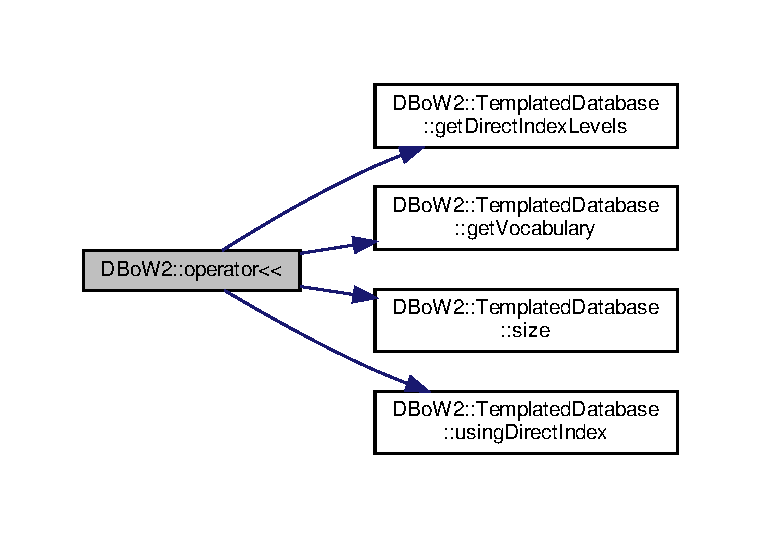
\includegraphics[width=350pt]{namespaceDBoW2_ac1f00f5484f61d6ab3b1f650955210d8_cgraph}
\end{center}
\end{figure}
\mbox{\Hypertarget{namespaceDBoW2_aecdf616fe16d2cf09f521a603b9d43f1}\label{namespaceDBoW2_aecdf616fe16d2cf09f521a603b9d43f1}} 
\index{D\+Bo\+W2@{D\+Bo\+W2}!operator$<$$<$@{operator$<$$<$}}
\index{operator$<$$<$@{operator$<$$<$}!D\+Bo\+W2@{D\+Bo\+W2}}
\subsubsection{\texorpdfstring{operator$<$$<$()}{operator<<()}\hspace{0.1cm}{\footnotesize\ttfamily [4/4]}}
{\footnotesize\ttfamily template$<$class T\+Descriptor , class F $>$ \\
std\+::ostream\& D\+Bo\+W2\+::operator$<$$<$ (\begin{DoxyParamCaption}\item[{std\+::ostream \&}]{os,  }\item[{const \hyperlink{classDBoW2_1_1TemplatedVocabulary}{Templated\+Vocabulary}$<$ T\+Descriptor, F $>$ \&}]{voc }\end{DoxyParamCaption})}

Writes printable information of the vocabulary 
\begin{DoxyParams}{Parameters}
{\em os} & stream to write to \\
\hline
{\em voc} & \\
\hline
\end{DoxyParams}


References D\+Bo\+W2\+::\+Templated\+Vocabulary$<$ T\+Descriptor, F $>$\+::get\+Branching\+Factor(), D\+Bo\+W2\+::\+Templated\+Vocabulary$<$ T\+Descriptor, F $>$\+::get\+Depth\+Levels(), D\+Bo\+W2\+::\+Templated\+Vocabulary$<$ T\+Descriptor, F $>$\+::get\+Scoring\+Type(), D\+Bo\+W2\+::\+Templated\+Vocabulary$<$ T\+Descriptor, F $>$\+::get\+Weighting\+Type(), and D\+Bo\+W2\+::\+Templated\+Vocabulary$<$ T\+Descriptor, F $>$\+::size().

Here is the call graph for this function\+:\nopagebreak
\begin{figure}[H]
\begin{center}
\leavevmode
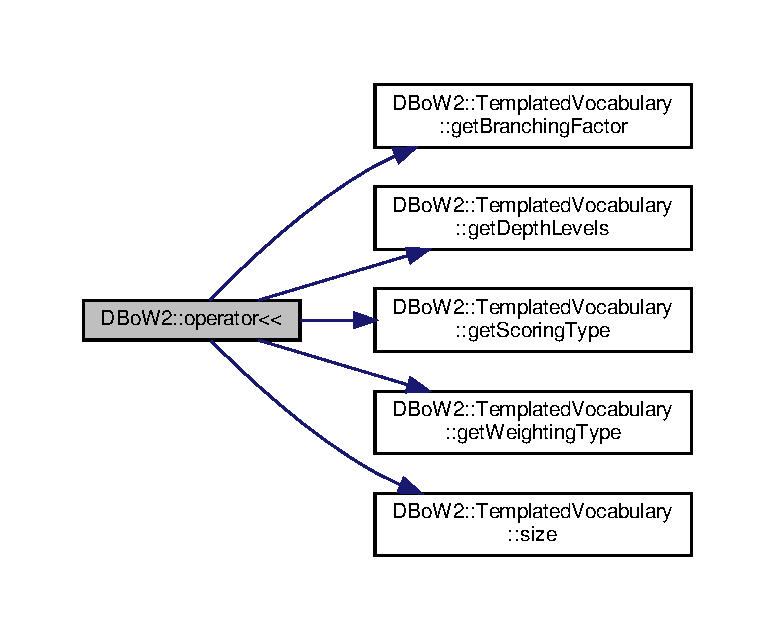
\includegraphics[width=350pt]{namespaceDBoW2_aecdf616fe16d2cf09f521a603b9d43f1_cgraph}
\end{center}
\end{figure}

\hypertarget{namespaceDUtils}{}\section{D\+Utils Namespace Reference}
\label{namespaceDUtils}\index{D\+Utils@{D\+Utils}}


Several utilities for C++ programs.  


\subsection*{Classes}
\begin{DoxyCompactItemize}
\item 
class \hyperlink{classDUtils_1_1DException}{D\+Exception}
\begin{DoxyCompactList}\small\item\em General exception. \end{DoxyCompactList}\item 
class \hyperlink{classDUtils_1_1Random}{Random}
\begin{DoxyCompactList}\small\item\em Functions to generate pseudo-\/random numbers. \end{DoxyCompactList}\item 
class \hyperlink{classDUtils_1_1Timestamp}{Timestamp}
\begin{DoxyCompactList}\small\item\em \hyperlink{classDUtils_1_1Timestamp}{Timestamp}. \end{DoxyCompactList}\end{DoxyCompactItemize}


\subsection{Detailed Description}
Several utilities for C++ programs. 
\hypertarget{namespaceDVision}{}\section{D\+Vision Namespace Reference}
\label{namespaceDVision}\index{D\+Vision@{D\+Vision}}


Computer vision functions.  


\subsection*{Classes}
\begin{DoxyCompactItemize}
\item 
class \hyperlink{classDVision_1_1BRIEF}{B\+R\+I\+EF}
\begin{DoxyCompactList}\small\item\em \hyperlink{classDVision_1_1BRIEF}{B\+R\+I\+EF} descriptor. \end{DoxyCompactList}\end{DoxyCompactItemize}


\subsection{Detailed Description}
Computer vision functions. 

File\+: \hyperlink{BRIEF_8h_source}{B\+R\+I\+E\+F.\+h} Author\+: Dorian Galvez-\/\+Lopez Date\+: March 2011 Description\+: implementation of \hyperlink{classDVision_1_1BRIEF}{B\+R\+I\+EF} (Binary Robust Independent Elementary Features) descriptor by Michael Calonder, Vincent Lepetit and Pascal Fua
\begin{DoxyItemize}
\item close binary tests (by Dorian Galvez-\/\+Lopez)
\end{DoxyItemize}

If you use this code with the R\+A\+N\+D\+O\+M\+\_\+\+C\+L\+O\+SE descriptor version, please cite\+: \{Galvez\+I\+R\+O\+S11, author=\{Galvez-\/\+Lopez, Dorian and Tardos, Juan D.\}, booktitle=\{Intelligent Robots and Systems (I\+R\+OS), 2011 I\+E\+E\+E/\+R\+SJ International Conference on\}, title=\{Real-\/time loop detection with bags of binary words\}, year=\{2011\}, month=\{sept.\}, volume=\{\}, number=\{\}, pages=\{51 -\/58\}, keywords=\{\}, doi=\{10.\+1109/\+I\+R\+OS.2011.\+6094885\}, I\+S\+SN=\{2153-\/0858\} \}

License\+: see the L\+I\+C\+E\+N\+S\+E.\+txt file 
\chapter{Class Documentation}
\hypertarget{classAngleLocalParameterization}{}\section{Angle\+Local\+Parameterization Class Reference}
\label{classAngleLocalParameterization}\index{Angle\+Local\+Parameterization@{Angle\+Local\+Parameterization}}
\subsection*{Public Member Functions}
\begin{DoxyCompactItemize}
\item 
\mbox{\Hypertarget{classAngleLocalParameterization_ac2debe098dab8a96bbee0c6057997a86}\label{classAngleLocalParameterization_ac2debe098dab8a96bbee0c6057997a86}} 
{\footnotesize template$<$typename T $>$ }\\bool {\bfseries operator()} (const T $\ast$theta\+\_\+radians, const T $\ast$delta\+\_\+theta\+\_\+radians, T $\ast$theta\+\_\+radians\+\_\+plus\+\_\+delta) const
\end{DoxyCompactItemize}
\subsection*{Static Public Member Functions}
\begin{DoxyCompactItemize}
\item 
\mbox{\Hypertarget{classAngleLocalParameterization_a73006f5f3280d4adccfa3612f8188868}\label{classAngleLocalParameterization_a73006f5f3280d4adccfa3612f8188868}} 
static ceres\+::\+Local\+Parameterization $\ast$ {\bfseries Create} ()
\end{DoxyCompactItemize}


The documentation for this class was generated from the following file\+:\begin{DoxyCompactItemize}
\item 
pose\+\_\+graph/src/pose\+\_\+graph.\+h\end{DoxyCompactItemize}

\hypertarget{classDBoW2_1_1BowVector}{}\section{D\+Bo\+W2\+:\+:Bow\+Vector Class Reference}
\label{classDBoW2_1_1BowVector}\index{D\+Bo\+W2\+::\+Bow\+Vector@{D\+Bo\+W2\+::\+Bow\+Vector}}


Vector of words to represent images.  




{\ttfamily \#include $<$Bow\+Vector.\+h$>$}



Inheritance diagram for D\+Bo\+W2\+:\+:Bow\+Vector\+:\nopagebreak
\begin{figure}[H]
\begin{center}
\leavevmode
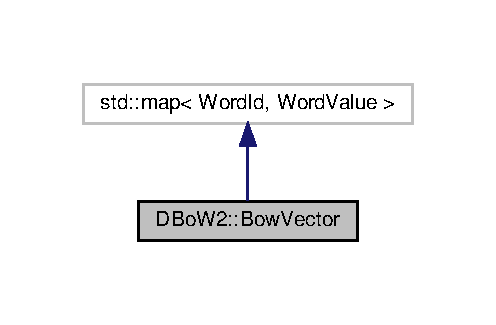
\includegraphics[width=238pt]{classDBoW2_1_1BowVector__inherit__graph}
\end{center}
\end{figure}


Collaboration diagram for D\+Bo\+W2\+:\+:Bow\+Vector\+:\nopagebreak
\begin{figure}[H]
\begin{center}
\leavevmode
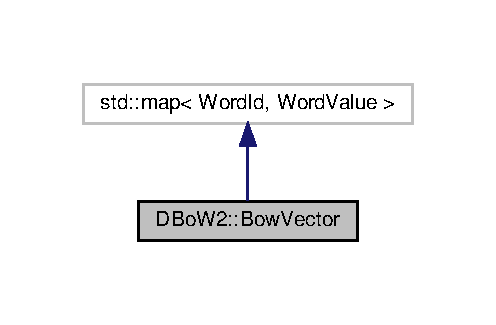
\includegraphics[width=238pt]{classDBoW2_1_1BowVector__coll__graph}
\end{center}
\end{figure}
\subsection*{Public Member Functions}
\begin{DoxyCompactItemize}
\item 
\hyperlink{classDBoW2_1_1BowVector_ac4da23e700adc4ee083d66b23ce86e90}{Bow\+Vector} (void)
\item 
\hyperlink{classDBoW2_1_1BowVector_a7210cac6ce006c7232f4d097faa338d0}{$\sim$\+Bow\+Vector} (void)
\item 
void \hyperlink{classDBoW2_1_1BowVector_a3ac92a805b252c93dc6535240d02df47}{add\+Weight} (\hyperlink{namespaceDBoW2_ab1a0d3283b2d4690a383372ed20bfeb5}{Word\+Id} id, \hyperlink{namespaceDBoW2_a55fcd7333e591a38e96b91f41bc182f6}{Word\+Value} v)
\item 
void \hyperlink{classDBoW2_1_1BowVector_a5ddf10e444d10425e5bd3568dc7ffe5e}{add\+If\+Not\+Exist} (\hyperlink{namespaceDBoW2_ab1a0d3283b2d4690a383372ed20bfeb5}{Word\+Id} id, \hyperlink{namespaceDBoW2_a55fcd7333e591a38e96b91f41bc182f6}{Word\+Value} v)
\item 
void \hyperlink{classDBoW2_1_1BowVector_acd2dd34023e3053a4cc75d70c8b6ac13}{normalize} (\hyperlink{namespaceDBoW2_a53e9e0bcfc25c861815e413a7cf3fa51}{L\+Norm} norm\+\_\+type)
\item 
void \hyperlink{classDBoW2_1_1BowVector_a0611e948f987574161c121231341537b}{saveM} (const std\+::string \&filename, size\+\_\+t W) const
\end{DoxyCompactItemize}
\subsection*{Friends}
\begin{DoxyCompactItemize}
\item 
std\+::ostream \& \hyperlink{classDBoW2_1_1BowVector_a1a7d9ac0f9128538859adfea38453ae1}{operator$<$$<$} (std\+::ostream \&out, const \hyperlink{classDBoW2_1_1BowVector}{Bow\+Vector} \&v)
\end{DoxyCompactItemize}


\subsection{Detailed Description}
Vector of words to represent images. 

\subsection{Constructor \& Destructor Documentation}
\mbox{\Hypertarget{classDBoW2_1_1BowVector_ac4da23e700adc4ee083d66b23ce86e90}\label{classDBoW2_1_1BowVector_ac4da23e700adc4ee083d66b23ce86e90}} 
\index{D\+Bo\+W2\+::\+Bow\+Vector@{D\+Bo\+W2\+::\+Bow\+Vector}!Bow\+Vector@{Bow\+Vector}}
\index{Bow\+Vector@{Bow\+Vector}!D\+Bo\+W2\+::\+Bow\+Vector@{D\+Bo\+W2\+::\+Bow\+Vector}}
\subsubsection{\texorpdfstring{Bow\+Vector()}{BowVector()}}
{\footnotesize\ttfamily D\+Bo\+W2\+::\+Bow\+Vector\+::\+Bow\+Vector (\begin{DoxyParamCaption}\item[{void}]{ }\end{DoxyParamCaption})}

Constructor \mbox{\Hypertarget{classDBoW2_1_1BowVector_a7210cac6ce006c7232f4d097faa338d0}\label{classDBoW2_1_1BowVector_a7210cac6ce006c7232f4d097faa338d0}} 
\index{D\+Bo\+W2\+::\+Bow\+Vector@{D\+Bo\+W2\+::\+Bow\+Vector}!````~Bow\+Vector@{$\sim$\+Bow\+Vector}}
\index{````~Bow\+Vector@{$\sim$\+Bow\+Vector}!D\+Bo\+W2\+::\+Bow\+Vector@{D\+Bo\+W2\+::\+Bow\+Vector}}
\subsubsection{\texorpdfstring{$\sim$\+Bow\+Vector()}{~BowVector()}}
{\footnotesize\ttfamily D\+Bo\+W2\+::\+Bow\+Vector\+::$\sim$\+Bow\+Vector (\begin{DoxyParamCaption}\item[{void}]{ }\end{DoxyParamCaption})}

Destructor 

\subsection{Member Function Documentation}
\mbox{\Hypertarget{classDBoW2_1_1BowVector_a5ddf10e444d10425e5bd3568dc7ffe5e}\label{classDBoW2_1_1BowVector_a5ddf10e444d10425e5bd3568dc7ffe5e}} 
\index{D\+Bo\+W2\+::\+Bow\+Vector@{D\+Bo\+W2\+::\+Bow\+Vector}!add\+If\+Not\+Exist@{add\+If\+Not\+Exist}}
\index{add\+If\+Not\+Exist@{add\+If\+Not\+Exist}!D\+Bo\+W2\+::\+Bow\+Vector@{D\+Bo\+W2\+::\+Bow\+Vector}}
\subsubsection{\texorpdfstring{add\+If\+Not\+Exist()}{addIfNotExist()}}
{\footnotesize\ttfamily void D\+Bo\+W2\+::\+Bow\+Vector\+::add\+If\+Not\+Exist (\begin{DoxyParamCaption}\item[{\hyperlink{namespaceDBoW2_ab1a0d3283b2d4690a383372ed20bfeb5}{Word\+Id}}]{id,  }\item[{\hyperlink{namespaceDBoW2_a55fcd7333e591a38e96b91f41bc182f6}{Word\+Value}}]{v }\end{DoxyParamCaption})}

Adds a word with a value to the vector only if this does not exist yet 
\begin{DoxyParams}{Parameters}
{\em id} & word id to look for \\
\hline
{\em v} & value to give to the word if this does not exist \\
\hline
\end{DoxyParams}


Referenced by D\+Bo\+W2\+::\+Templated\+Vocabulary$<$ D\+Bo\+W2\+::\+F\+Brief\+::\+T\+Descriptor, D\+Bo\+W2\+::\+F\+Brief $>$\+::transform().

Here is the caller graph for this function\+:\nopagebreak
\begin{figure}[H]
\begin{center}
\leavevmode
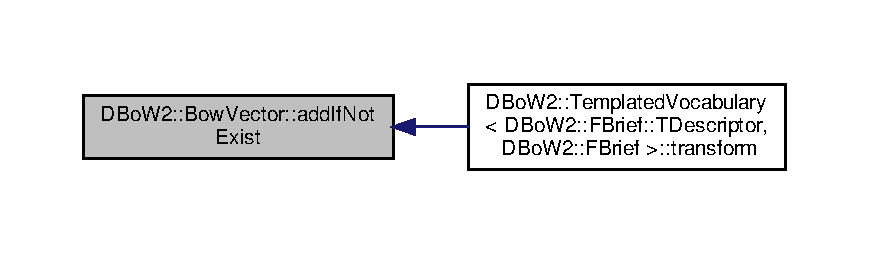
\includegraphics[width=350pt]{classDBoW2_1_1BowVector_a5ddf10e444d10425e5bd3568dc7ffe5e_icgraph}
\end{center}
\end{figure}
\mbox{\Hypertarget{classDBoW2_1_1BowVector_a3ac92a805b252c93dc6535240d02df47}\label{classDBoW2_1_1BowVector_a3ac92a805b252c93dc6535240d02df47}} 
\index{D\+Bo\+W2\+::\+Bow\+Vector@{D\+Bo\+W2\+::\+Bow\+Vector}!add\+Weight@{add\+Weight}}
\index{add\+Weight@{add\+Weight}!D\+Bo\+W2\+::\+Bow\+Vector@{D\+Bo\+W2\+::\+Bow\+Vector}}
\subsubsection{\texorpdfstring{add\+Weight()}{addWeight()}}
{\footnotesize\ttfamily void D\+Bo\+W2\+::\+Bow\+Vector\+::add\+Weight (\begin{DoxyParamCaption}\item[{\hyperlink{namespaceDBoW2_ab1a0d3283b2d4690a383372ed20bfeb5}{Word\+Id}}]{id,  }\item[{\hyperlink{namespaceDBoW2_a55fcd7333e591a38e96b91f41bc182f6}{Word\+Value}}]{v }\end{DoxyParamCaption})}

Adds a value to a word value existing in the vector, or creates a new word with the given value 
\begin{DoxyParams}{Parameters}
{\em id} & word id to look for \\
\hline
{\em v} & value to create the word with, or to add to existing word \\
\hline
\end{DoxyParams}


Referenced by D\+Bo\+W2\+::\+Templated\+Vocabulary$<$ D\+Bo\+W2\+::\+F\+Brief\+::\+T\+Descriptor, D\+Bo\+W2\+::\+F\+Brief $>$\+::transform().

Here is the caller graph for this function\+:\nopagebreak
\begin{figure}[H]
\begin{center}
\leavevmode
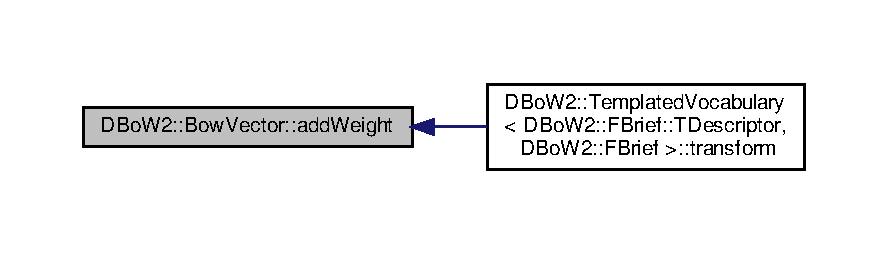
\includegraphics[width=350pt]{classDBoW2_1_1BowVector_a3ac92a805b252c93dc6535240d02df47_icgraph}
\end{center}
\end{figure}
\mbox{\Hypertarget{classDBoW2_1_1BowVector_acd2dd34023e3053a4cc75d70c8b6ac13}\label{classDBoW2_1_1BowVector_acd2dd34023e3053a4cc75d70c8b6ac13}} 
\index{D\+Bo\+W2\+::\+Bow\+Vector@{D\+Bo\+W2\+::\+Bow\+Vector}!normalize@{normalize}}
\index{normalize@{normalize}!D\+Bo\+W2\+::\+Bow\+Vector@{D\+Bo\+W2\+::\+Bow\+Vector}}
\subsubsection{\texorpdfstring{normalize()}{normalize()}}
{\footnotesize\ttfamily void D\+Bo\+W2\+::\+Bow\+Vector\+::normalize (\begin{DoxyParamCaption}\item[{\hyperlink{namespaceDBoW2_a53e9e0bcfc25c861815e413a7cf3fa51}{L\+Norm}}]{norm\+\_\+type }\end{DoxyParamCaption})}

L1-\/\+Normalizes the values in the vector 
\begin{DoxyParams}{Parameters}
{\em norm\+\_\+type} & norm used \\
\hline
\end{DoxyParams}


Referenced by D\+Bo\+W2\+::\+Templated\+Vocabulary$<$ D\+Bo\+W2\+::\+F\+Brief\+::\+T\+Descriptor, D\+Bo\+W2\+::\+F\+Brief $>$\+::transform().

Here is the caller graph for this function\+:\nopagebreak
\begin{figure}[H]
\begin{center}
\leavevmode
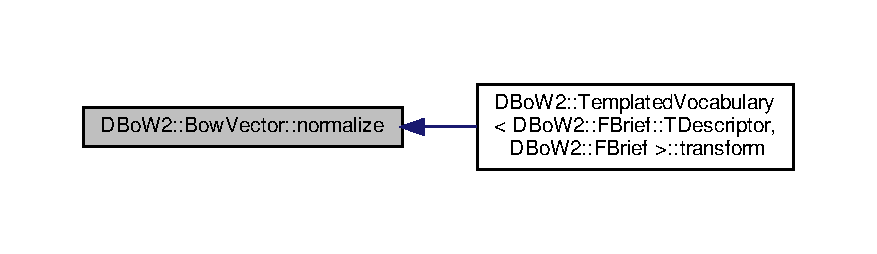
\includegraphics[width=350pt]{classDBoW2_1_1BowVector_acd2dd34023e3053a4cc75d70c8b6ac13_icgraph}
\end{center}
\end{figure}
\mbox{\Hypertarget{classDBoW2_1_1BowVector_a0611e948f987574161c121231341537b}\label{classDBoW2_1_1BowVector_a0611e948f987574161c121231341537b}} 
\index{D\+Bo\+W2\+::\+Bow\+Vector@{D\+Bo\+W2\+::\+Bow\+Vector}!saveM@{saveM}}
\index{saveM@{saveM}!D\+Bo\+W2\+::\+Bow\+Vector@{D\+Bo\+W2\+::\+Bow\+Vector}}
\subsubsection{\texorpdfstring{save\+M()}{saveM()}}
{\footnotesize\ttfamily void D\+Bo\+W2\+::\+Bow\+Vector\+::saveM (\begin{DoxyParamCaption}\item[{const std\+::string \&}]{filename,  }\item[{size\+\_\+t}]{W }\end{DoxyParamCaption}) const}

Saves the bow vector as a vector in a matlab file 
\begin{DoxyParams}{Parameters}
{\em filename} & \\
\hline
{\em W} & number of words in the vocabulary \\
\hline
\end{DoxyParams}


\subsection{Friends And Related Function Documentation}
\mbox{\Hypertarget{classDBoW2_1_1BowVector_a1a7d9ac0f9128538859adfea38453ae1}\label{classDBoW2_1_1BowVector_a1a7d9ac0f9128538859adfea38453ae1}} 
\index{D\+Bo\+W2\+::\+Bow\+Vector@{D\+Bo\+W2\+::\+Bow\+Vector}!operator$<$$<$@{operator$<$$<$}}
\index{operator$<$$<$@{operator$<$$<$}!D\+Bo\+W2\+::\+Bow\+Vector@{D\+Bo\+W2\+::\+Bow\+Vector}}
\subsubsection{\texorpdfstring{operator$<$$<$}{operator<<}}
{\footnotesize\ttfamily std\+::ostream\& operator$<$$<$ (\begin{DoxyParamCaption}\item[{std\+::ostream \&}]{out,  }\item[{const \hyperlink{classDBoW2_1_1BowVector}{Bow\+Vector} \&}]{v }\end{DoxyParamCaption})\hspace{0.3cm}{\ttfamily [friend]}}

Prints the content of the bow vector 
\begin{DoxyParams}{Parameters}
{\em out} & stream \\
\hline
{\em v} & \\
\hline
\end{DoxyParams}


The documentation for this class was generated from the following files\+:\begin{DoxyCompactItemize}
\item 
pose\+\_\+graph/src/\+Third\+Party/\+D\+Bo\+W/Bow\+Vector.\+h\item 
pose\+\_\+graph/src/\+Third\+Party/\+D\+Bo\+W/Bow\+Vector.\+cpp\end{DoxyCompactItemize}

\hypertarget{classDVision_1_1BRIEF}{}\section{D\+Vision\+:\+:B\+R\+I\+EF Class Reference}
\label{classDVision_1_1BRIEF}\index{D\+Vision\+::\+B\+R\+I\+EF@{D\+Vision\+::\+B\+R\+I\+EF}}


\hyperlink{classDVision_1_1BRIEF}{B\+R\+I\+EF} descriptor.  




{\ttfamily \#include $<$B\+R\+I\+E\+F.\+h$>$}

\subsection*{Public Types}
\begin{DoxyCompactItemize}
\item 
\mbox{\Hypertarget{classDVision_1_1BRIEF_a0203beaaafe3aca790393cc032eeb499}\label{classDVision_1_1BRIEF_a0203beaaafe3aca790393cc032eeb499}} 
enum \hyperlink{classDVision_1_1BRIEF_a0203beaaafe3aca790393cc032eeb499}{Type} \{ {\bfseries R\+A\+N\+D\+OM}, 
{\bfseries R\+A\+N\+D\+O\+M\+\_\+\+C\+L\+O\+SE}
 \}\begin{DoxyCompactList}\small\item\em Type of pairs. \end{DoxyCompactList}
\item 
\mbox{\Hypertarget{classDVision_1_1BRIEF_abc56a095174a93b0741099f35230b7c5}\label{classDVision_1_1BRIEF_abc56a095174a93b0741099f35230b7c5}} 
typedef boost\+::dynamic\+\_\+bitset \hyperlink{classDVision_1_1BRIEF_abc56a095174a93b0741099f35230b7c5}{bitset}
\begin{DoxyCompactList}\small\item\em Bitset type. \end{DoxyCompactList}\end{DoxyCompactItemize}
\subsection*{Public Member Functions}
\begin{DoxyCompactItemize}
\item 
\hyperlink{classDVision_1_1BRIEF_a4dd74c26a2e1f4cb938f75fdad3e88cf}{B\+R\+I\+EF} (int nbits=256, int patch\+\_\+size=48, \hyperlink{classDVision_1_1BRIEF_a0203beaaafe3aca790393cc032eeb499}{Type} type=R\+A\+N\+D\+O\+M\+\_\+\+C\+L\+O\+SE)
\item 
int \hyperlink{classDVision_1_1BRIEF_aa7679cb7d06344d75e4375baf779b84c}{get\+Descriptor\+Length\+In\+Bits} () const
\item 
\hyperlink{classDVision_1_1BRIEF_a0203beaaafe3aca790393cc032eeb499}{Type} \hyperlink{classDVision_1_1BRIEF_ad2b1b7422d05905597e31939528cbd2a}{get\+Type} () const
\item 
int \hyperlink{classDVision_1_1BRIEF_aabaa4937582b567fa1f53ec6004cfc00}{get\+Patch\+Size} () const
\item 
void \hyperlink{classDVision_1_1BRIEF_a290ee93994c09ed3b2164c5d3df182a9}{operator()} (const cv\+::\+Mat \&image, const std\+::vector$<$ cv\+::\+Key\+Point $>$ \&points, std\+::vector$<$ \hyperlink{classDVision_1_1BRIEF_abc56a095174a93b0741099f35230b7c5}{bitset} $>$ \&descriptors, bool treat\+\_\+image=true) const
\item 
void \hyperlink{classDVision_1_1BRIEF_afda5792d22d954fabbadeed3388ca6c7}{compute} (const cv\+::\+Mat \&image, const std\+::vector$<$ cv\+::\+Key\+Point $>$ \&points, std\+::vector$<$ \hyperlink{classDVision_1_1BRIEF_abc56a095174a93b0741099f35230b7c5}{bitset} $>$ \&descriptors, bool treat\+\_\+image=true) const
\item 
void \hyperlink{classDVision_1_1BRIEF_a8000a709f6336e47359c6e9ee4a5efd5}{export\+Pairs} (std\+::vector$<$ int $>$ \&x1, std\+::vector$<$ int $>$ \&y1, std\+::vector$<$ int $>$ \&x2, std\+::vector$<$ int $>$ \&y2) const
\item 
void \hyperlink{classDVision_1_1BRIEF_a019cd2ef2f6757da94fdb1f74d20b581}{import\+Pairs} (const std\+::vector$<$ int $>$ \&x1, const std\+::vector$<$ int $>$ \&y1, const std\+::vector$<$ int $>$ \&x2, const std\+::vector$<$ int $>$ \&y2)
\end{DoxyCompactItemize}
\subsection*{Static Public Member Functions}
\begin{DoxyCompactItemize}
\item 
static int \hyperlink{classDVision_1_1BRIEF_a78718071fcf2700e3a0cc304dd4e1dcc}{distance} (const \hyperlink{classDVision_1_1BRIEF_abc56a095174a93b0741099f35230b7c5}{bitset} \&a, const \hyperlink{classDVision_1_1BRIEF_abc56a095174a93b0741099f35230b7c5}{bitset} \&b)
\end{DoxyCompactItemize}
\subsection*{Protected Member Functions}
\begin{DoxyCompactItemize}
\item 
void \hyperlink{classDVision_1_1BRIEF_a6daf52c01b9cbd845151077837870283}{generate\+Test\+Points} ()
\end{DoxyCompactItemize}
\subsection*{Protected Attributes}
\begin{DoxyCompactItemize}
\item 
\mbox{\Hypertarget{classDVision_1_1BRIEF_ae49b641f3fd2f58928e1256627b4bb21}\label{classDVision_1_1BRIEF_ae49b641f3fd2f58928e1256627b4bb21}} 
int \hyperlink{classDVision_1_1BRIEF_ae49b641f3fd2f58928e1256627b4bb21}{m\+\_\+bit\+\_\+length}
\begin{DoxyCompactList}\small\item\em Descriptor length in bits. \end{DoxyCompactList}\item 
\mbox{\Hypertarget{classDVision_1_1BRIEF_a73fca9548bbf58380cacedc73e4b5c0b}\label{classDVision_1_1BRIEF_a73fca9548bbf58380cacedc73e4b5c0b}} 
int \hyperlink{classDVision_1_1BRIEF_a73fca9548bbf58380cacedc73e4b5c0b}{m\+\_\+patch\+\_\+size}
\begin{DoxyCompactList}\small\item\em Patch size. \end{DoxyCompactList}\item 
\mbox{\Hypertarget{classDVision_1_1BRIEF_aaf2f0e2289b6924b32ecafb7b94bd9ff}\label{classDVision_1_1BRIEF_aaf2f0e2289b6924b32ecafb7b94bd9ff}} 
\hyperlink{classDVision_1_1BRIEF_a0203beaaafe3aca790393cc032eeb499}{Type} \hyperlink{classDVision_1_1BRIEF_aaf2f0e2289b6924b32ecafb7b94bd9ff}{m\+\_\+type}
\begin{DoxyCompactList}\small\item\em Type of pairs. \end{DoxyCompactList}\item 
\mbox{\Hypertarget{classDVision_1_1BRIEF_a406548dc5cddec3b105d6ab35beadb40}\label{classDVision_1_1BRIEF_a406548dc5cddec3b105d6ab35beadb40}} 
std\+::vector$<$ int $>$ \hyperlink{classDVision_1_1BRIEF_a406548dc5cddec3b105d6ab35beadb40}{m\+\_\+x1}
\begin{DoxyCompactList}\small\item\em Coordinates of test points relative to the center of the patch. \end{DoxyCompactList}\item 
\mbox{\Hypertarget{classDVision_1_1BRIEF_a8b2c44f32eb3d0f388d5daf80113426a}\label{classDVision_1_1BRIEF_a8b2c44f32eb3d0f388d5daf80113426a}} 
std\+::vector$<$ int $>$ {\bfseries m\+\_\+x2}
\item 
\mbox{\Hypertarget{classDVision_1_1BRIEF_a608e4ed7c763351804f22f3a0fc55bb0}\label{classDVision_1_1BRIEF_a608e4ed7c763351804f22f3a0fc55bb0}} 
std\+::vector$<$ int $>$ {\bfseries m\+\_\+y1}
\item 
\mbox{\Hypertarget{classDVision_1_1BRIEF_a4c5fdb95b1880316f8a7527912319ad0}\label{classDVision_1_1BRIEF_a4c5fdb95b1880316f8a7527912319ad0}} 
std\+::vector$<$ int $>$ {\bfseries m\+\_\+y2}
\end{DoxyCompactItemize}


\subsection{Detailed Description}
\hyperlink{classDVision_1_1BRIEF}{B\+R\+I\+EF} descriptor. 

\subsection{Constructor \& Destructor Documentation}
\mbox{\Hypertarget{classDVision_1_1BRIEF_a4dd74c26a2e1f4cb938f75fdad3e88cf}\label{classDVision_1_1BRIEF_a4dd74c26a2e1f4cb938f75fdad3e88cf}} 
\index{D\+Vision\+::\+B\+R\+I\+EF@{D\+Vision\+::\+B\+R\+I\+EF}!B\+R\+I\+EF@{B\+R\+I\+EF}}
\index{B\+R\+I\+EF@{B\+R\+I\+EF}!D\+Vision\+::\+B\+R\+I\+EF@{D\+Vision\+::\+B\+R\+I\+EF}}
\subsubsection{\texorpdfstring{B\+R\+I\+E\+F()}{BRIEF()}}
{\footnotesize\ttfamily B\+R\+I\+E\+F\+::\+B\+R\+I\+EF (\begin{DoxyParamCaption}\item[{int}]{nbits = {\ttfamily 256},  }\item[{int}]{patch\+\_\+size = {\ttfamily 48},  }\item[{\hyperlink{classDVision_1_1BRIEF_a0203beaaafe3aca790393cc032eeb499}{Type}}]{type = {\ttfamily RANDOM\+\_\+CLOSE} }\end{DoxyParamCaption})}

Creates the \hyperlink{classDVision_1_1BRIEF}{B\+R\+I\+EF} a priori data for descriptors of nbits length 
\begin{DoxyParams}{Parameters}
{\em nbits} & descriptor length in bits \\
\hline
{\em patch\+\_\+size} & \\
\hline
{\em type} & type of pairs to generate \\
\hline
\end{DoxyParams}


References generate\+Test\+Points().

Here is the call graph for this function\+:\nopagebreak
\begin{figure}[H]
\begin{center}
\leavevmode
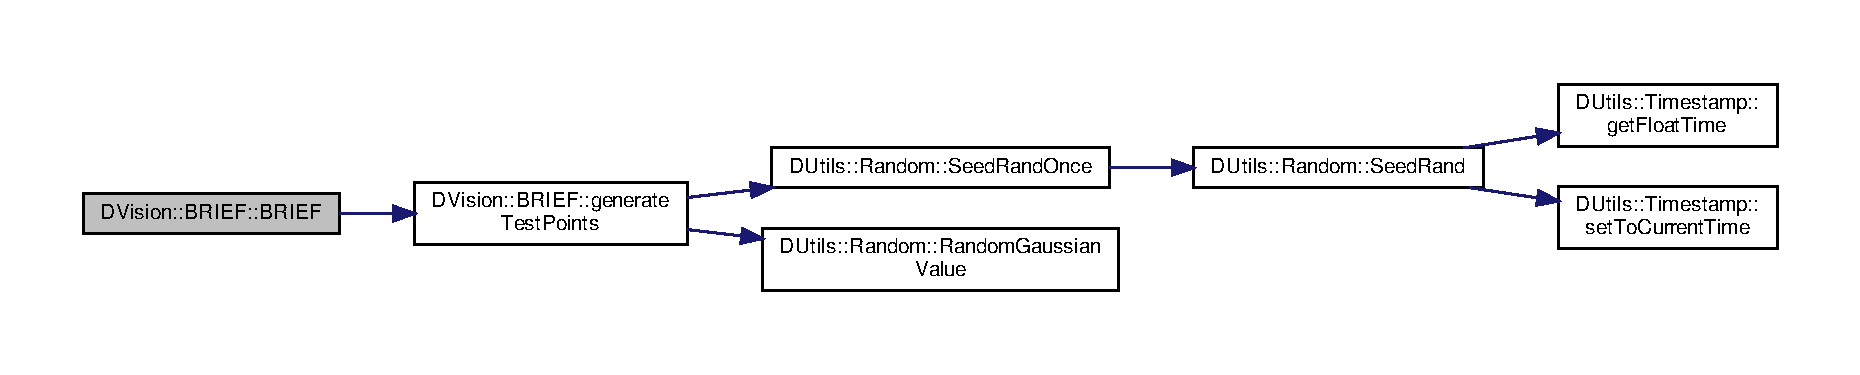
\includegraphics[width=350pt]{classDVision_1_1BRIEF_a4dd74c26a2e1f4cb938f75fdad3e88cf_cgraph}
\end{center}
\end{figure}


\subsection{Member Function Documentation}
\mbox{\Hypertarget{classDVision_1_1BRIEF_afda5792d22d954fabbadeed3388ca6c7}\label{classDVision_1_1BRIEF_afda5792d22d954fabbadeed3388ca6c7}} 
\index{D\+Vision\+::\+B\+R\+I\+EF@{D\+Vision\+::\+B\+R\+I\+EF}!compute@{compute}}
\index{compute@{compute}!D\+Vision\+::\+B\+R\+I\+EF@{D\+Vision\+::\+B\+R\+I\+EF}}
\subsubsection{\texorpdfstring{compute()}{compute()}}
{\footnotesize\ttfamily void B\+R\+I\+E\+F\+::compute (\begin{DoxyParamCaption}\item[{const cv\+::\+Mat \&}]{image,  }\item[{const std\+::vector$<$ cv\+::\+Key\+Point $>$ \&}]{points,  }\item[{std\+::vector$<$ \hyperlink{classDVision_1_1BRIEF_abc56a095174a93b0741099f35230b7c5}{bitset} $>$ \&}]{descriptors,  }\item[{bool}]{treat\+\_\+image = {\ttfamily true} }\end{DoxyParamCaption}) const}

Returns the \hyperlink{classDVision_1_1BRIEF}{B\+R\+I\+EF} descriptors of the given keypoints in the given image 
\begin{DoxyParams}{Parameters}
{\em image} & \\
\hline
{\em points} & \\
\hline
{\em descriptors} & \\
\hline
{\em treat\+\_\+image} & (default\+: true) if true, the image is converted to grayscale if needed and smoothed. If not, it is assumed the image has been treated by the user \\
\hline
\end{DoxyParams}
\begin{DoxyNote}{Note}
this function is similar to B\+R\+I\+E\+F\+::operator() 
\end{DoxyNote}


References m\+\_\+bit\+\_\+length, and m\+\_\+x1.



Referenced by operator()().

Here is the caller graph for this function\+:\nopagebreak
\begin{figure}[H]
\begin{center}
\leavevmode
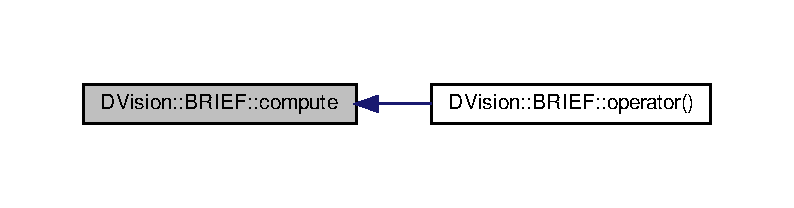
\includegraphics[width=350pt]{classDVision_1_1BRIEF_afda5792d22d954fabbadeed3388ca6c7_icgraph}
\end{center}
\end{figure}
\mbox{\Hypertarget{classDVision_1_1BRIEF_a78718071fcf2700e3a0cc304dd4e1dcc}\label{classDVision_1_1BRIEF_a78718071fcf2700e3a0cc304dd4e1dcc}} 
\index{D\+Vision\+::\+B\+R\+I\+EF@{D\+Vision\+::\+B\+R\+I\+EF}!distance@{distance}}
\index{distance@{distance}!D\+Vision\+::\+B\+R\+I\+EF@{D\+Vision\+::\+B\+R\+I\+EF}}
\subsubsection{\texorpdfstring{distance()}{distance()}}
{\footnotesize\ttfamily static int D\+Vision\+::\+B\+R\+I\+E\+F\+::distance (\begin{DoxyParamCaption}\item[{const \hyperlink{classDVision_1_1BRIEF_abc56a095174a93b0741099f35230b7c5}{bitset} \&}]{a,  }\item[{const \hyperlink{classDVision_1_1BRIEF_abc56a095174a93b0741099f35230b7c5}{bitset} \&}]{b }\end{DoxyParamCaption})\hspace{0.3cm}{\ttfamily [inline]}, {\ttfamily [static]}}

Returns the Hamming distance between two descriptors 
\begin{DoxyParams}{Parameters}
{\em a} & first descriptor vector \\
\hline
{\em b} & second descriptor vector \\
\hline
\end{DoxyParams}
\begin{DoxyReturn}{Returns}
hamming distance 
\end{DoxyReturn}


References generate\+Test\+Points().



Referenced by D\+Bo\+W2\+::\+F\+Brief\+::distance().

Here is the call graph for this function\+:\nopagebreak
\begin{figure}[H]
\begin{center}
\leavevmode
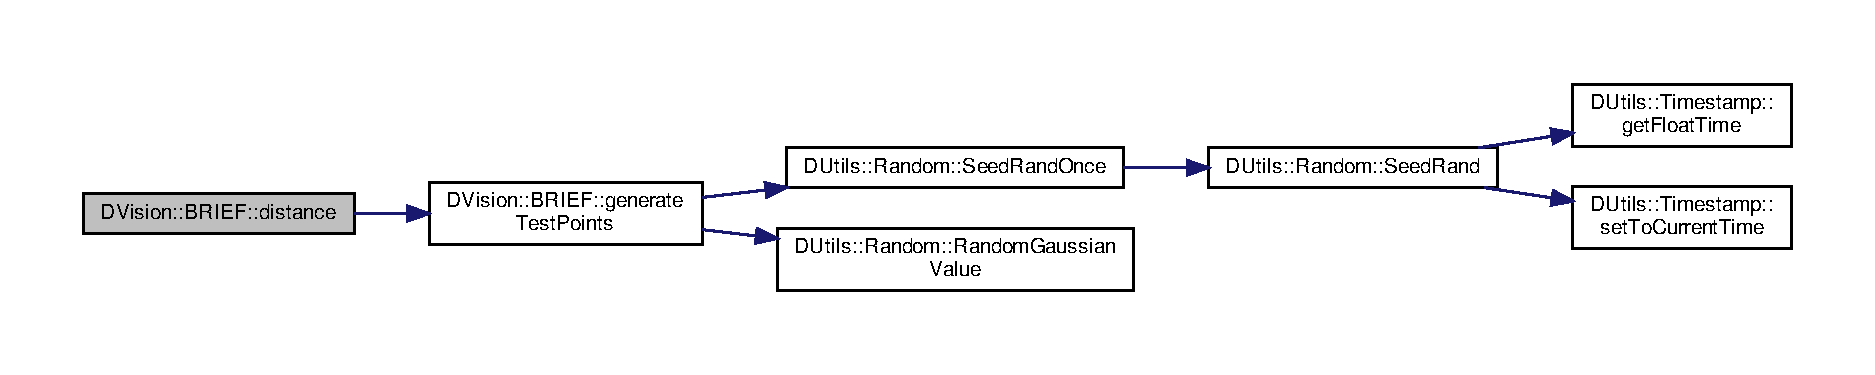
\includegraphics[width=350pt]{classDVision_1_1BRIEF_a78718071fcf2700e3a0cc304dd4e1dcc_cgraph}
\end{center}
\end{figure}
Here is the caller graph for this function\+:\nopagebreak
\begin{figure}[H]
\begin{center}
\leavevmode
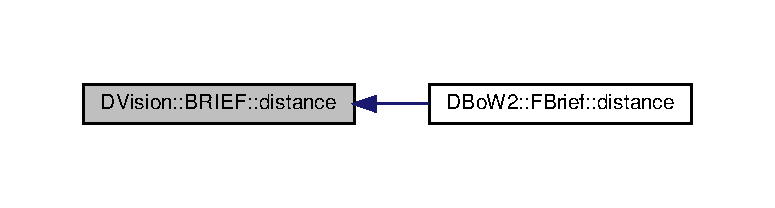
\includegraphics[width=350pt]{classDVision_1_1BRIEF_a78718071fcf2700e3a0cc304dd4e1dcc_icgraph}
\end{center}
\end{figure}
\mbox{\Hypertarget{classDVision_1_1BRIEF_a8000a709f6336e47359c6e9ee4a5efd5}\label{classDVision_1_1BRIEF_a8000a709f6336e47359c6e9ee4a5efd5}} 
\index{D\+Vision\+::\+B\+R\+I\+EF@{D\+Vision\+::\+B\+R\+I\+EF}!export\+Pairs@{export\+Pairs}}
\index{export\+Pairs@{export\+Pairs}!D\+Vision\+::\+B\+R\+I\+EF@{D\+Vision\+::\+B\+R\+I\+EF}}
\subsubsection{\texorpdfstring{export\+Pairs()}{exportPairs()}}
{\footnotesize\ttfamily void D\+Vision\+::\+B\+R\+I\+E\+F\+::export\+Pairs (\begin{DoxyParamCaption}\item[{std\+::vector$<$ int $>$ \&}]{x1,  }\item[{std\+::vector$<$ int $>$ \&}]{y1,  }\item[{std\+::vector$<$ int $>$ \&}]{x2,  }\item[{std\+::vector$<$ int $>$ \&}]{y2 }\end{DoxyParamCaption}) const\hspace{0.3cm}{\ttfamily [inline]}}

Exports the test pattern 
\begin{DoxyParams}{Parameters}
{\em x1} & x1 coordinates of pairs \\
\hline
{\em y1} & y1 coordinates of pairs \\
\hline
{\em x2} & x2 coordinates of pairs \\
\hline
{\em y2} & y2 coordinates of pairs \\
\hline
\end{DoxyParams}


References m\+\_\+x1.

\mbox{\Hypertarget{classDVision_1_1BRIEF_a6daf52c01b9cbd845151077837870283}\label{classDVision_1_1BRIEF_a6daf52c01b9cbd845151077837870283}} 
\index{D\+Vision\+::\+B\+R\+I\+EF@{D\+Vision\+::\+B\+R\+I\+EF}!generate\+Test\+Points@{generate\+Test\+Points}}
\index{generate\+Test\+Points@{generate\+Test\+Points}!D\+Vision\+::\+B\+R\+I\+EF@{D\+Vision\+::\+B\+R\+I\+EF}}
\subsubsection{\texorpdfstring{generate\+Test\+Points()}{generateTestPoints()}}
{\footnotesize\ttfamily void B\+R\+I\+E\+F\+::generate\+Test\+Points (\begin{DoxyParamCaption}{ }\end{DoxyParamCaption})\hspace{0.3cm}{\ttfamily [protected]}}

Generates random points in the patch coordinates, according to m\+\_\+patch\+\_\+size and m\+\_\+bit\+\_\+length 

References m\+\_\+bit\+\_\+length, m\+\_\+patch\+\_\+size, m\+\_\+type, m\+\_\+x1, D\+Utils\+::\+Random\+::\+Random\+Gaussian\+Value(), and D\+Utils\+::\+Random\+::\+Seed\+Rand\+Once().



Referenced by B\+R\+I\+E\+F(), and distance().

Here is the call graph for this function\+:\nopagebreak
\begin{figure}[H]
\begin{center}
\leavevmode
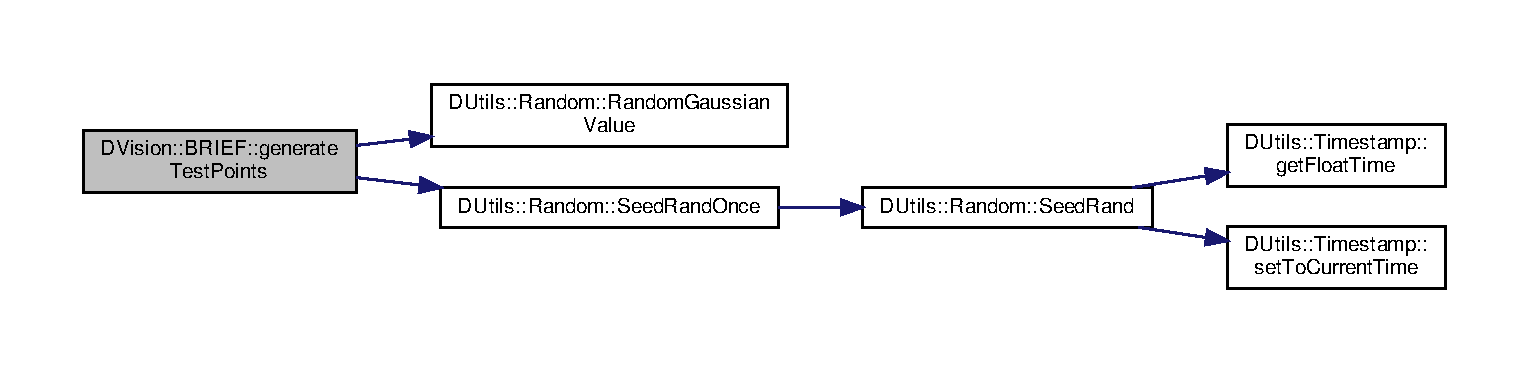
\includegraphics[width=350pt]{classDVision_1_1BRIEF_a6daf52c01b9cbd845151077837870283_cgraph}
\end{center}
\end{figure}
Here is the caller graph for this function\+:\nopagebreak
\begin{figure}[H]
\begin{center}
\leavevmode
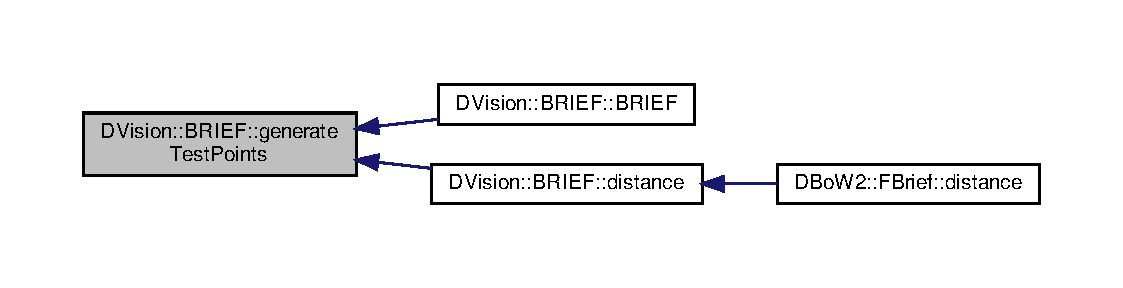
\includegraphics[width=350pt]{classDVision_1_1BRIEF_a6daf52c01b9cbd845151077837870283_icgraph}
\end{center}
\end{figure}
\mbox{\Hypertarget{classDVision_1_1BRIEF_aa7679cb7d06344d75e4375baf779b84c}\label{classDVision_1_1BRIEF_aa7679cb7d06344d75e4375baf779b84c}} 
\index{D\+Vision\+::\+B\+R\+I\+EF@{D\+Vision\+::\+B\+R\+I\+EF}!get\+Descriptor\+Length\+In\+Bits@{get\+Descriptor\+Length\+In\+Bits}}
\index{get\+Descriptor\+Length\+In\+Bits@{get\+Descriptor\+Length\+In\+Bits}!D\+Vision\+::\+B\+R\+I\+EF@{D\+Vision\+::\+B\+R\+I\+EF}}
\subsubsection{\texorpdfstring{get\+Descriptor\+Length\+In\+Bits()}{getDescriptorLengthInBits()}}
{\footnotesize\ttfamily int D\+Vision\+::\+B\+R\+I\+E\+F\+::get\+Descriptor\+Length\+In\+Bits (\begin{DoxyParamCaption}{ }\end{DoxyParamCaption}) const\hspace{0.3cm}{\ttfamily [inline]}}

Returns the descriptor length in bits \begin{DoxyReturn}{Returns}
descriptor length in bits 
\end{DoxyReturn}


References m\+\_\+bit\+\_\+length.

\mbox{\Hypertarget{classDVision_1_1BRIEF_aabaa4937582b567fa1f53ec6004cfc00}\label{classDVision_1_1BRIEF_aabaa4937582b567fa1f53ec6004cfc00}} 
\index{D\+Vision\+::\+B\+R\+I\+EF@{D\+Vision\+::\+B\+R\+I\+EF}!get\+Patch\+Size@{get\+Patch\+Size}}
\index{get\+Patch\+Size@{get\+Patch\+Size}!D\+Vision\+::\+B\+R\+I\+EF@{D\+Vision\+::\+B\+R\+I\+EF}}
\subsubsection{\texorpdfstring{get\+Patch\+Size()}{getPatchSize()}}
{\footnotesize\ttfamily int D\+Vision\+::\+B\+R\+I\+E\+F\+::get\+Patch\+Size (\begin{DoxyParamCaption}{ }\end{DoxyParamCaption}) const\hspace{0.3cm}{\ttfamily [inline]}}

Returns the size of the patch 

References m\+\_\+patch\+\_\+size.

\mbox{\Hypertarget{classDVision_1_1BRIEF_ad2b1b7422d05905597e31939528cbd2a}\label{classDVision_1_1BRIEF_ad2b1b7422d05905597e31939528cbd2a}} 
\index{D\+Vision\+::\+B\+R\+I\+EF@{D\+Vision\+::\+B\+R\+I\+EF}!get\+Type@{get\+Type}}
\index{get\+Type@{get\+Type}!D\+Vision\+::\+B\+R\+I\+EF@{D\+Vision\+::\+B\+R\+I\+EF}}
\subsubsection{\texorpdfstring{get\+Type()}{getType()}}
{\footnotesize\ttfamily \hyperlink{classDVision_1_1BRIEF_a0203beaaafe3aca790393cc032eeb499}{Type} D\+Vision\+::\+B\+R\+I\+E\+F\+::get\+Type (\begin{DoxyParamCaption}{ }\end{DoxyParamCaption}) const\hspace{0.3cm}{\ttfamily [inline]}}

Returns the type of classifier 

References m\+\_\+type.

\mbox{\Hypertarget{classDVision_1_1BRIEF_a019cd2ef2f6757da94fdb1f74d20b581}\label{classDVision_1_1BRIEF_a019cd2ef2f6757da94fdb1f74d20b581}} 
\index{D\+Vision\+::\+B\+R\+I\+EF@{D\+Vision\+::\+B\+R\+I\+EF}!import\+Pairs@{import\+Pairs}}
\index{import\+Pairs@{import\+Pairs}!D\+Vision\+::\+B\+R\+I\+EF@{D\+Vision\+::\+B\+R\+I\+EF}}
\subsubsection{\texorpdfstring{import\+Pairs()}{importPairs()}}
{\footnotesize\ttfamily void D\+Vision\+::\+B\+R\+I\+E\+F\+::import\+Pairs (\begin{DoxyParamCaption}\item[{const std\+::vector$<$ int $>$ \&}]{x1,  }\item[{const std\+::vector$<$ int $>$ \&}]{y1,  }\item[{const std\+::vector$<$ int $>$ \&}]{x2,  }\item[{const std\+::vector$<$ int $>$ \&}]{y2 }\end{DoxyParamCaption})\hspace{0.3cm}{\ttfamily [inline]}}

Sets the test pattern 
\begin{DoxyParams}{Parameters}
{\em x1} & x1 coordinates of pairs \\
\hline
{\em y1} & y1 coordinates of pairs \\
\hline
{\em x2} & x2 coordinates of pairs \\
\hline
{\em y2} & y2 coordinates of pairs \\
\hline
\end{DoxyParams}


References m\+\_\+bit\+\_\+length, and m\+\_\+x1.

\mbox{\Hypertarget{classDVision_1_1BRIEF_a290ee93994c09ed3b2164c5d3df182a9}\label{classDVision_1_1BRIEF_a290ee93994c09ed3b2164c5d3df182a9}} 
\index{D\+Vision\+::\+B\+R\+I\+EF@{D\+Vision\+::\+B\+R\+I\+EF}!operator()@{operator()}}
\index{operator()@{operator()}!D\+Vision\+::\+B\+R\+I\+EF@{D\+Vision\+::\+B\+R\+I\+EF}}
\subsubsection{\texorpdfstring{operator()()}{operator()()}}
{\footnotesize\ttfamily void D\+Vision\+::\+B\+R\+I\+E\+F\+::operator() (\begin{DoxyParamCaption}\item[{const cv\+::\+Mat \&}]{image,  }\item[{const std\+::vector$<$ cv\+::\+Key\+Point $>$ \&}]{points,  }\item[{std\+::vector$<$ \hyperlink{classDVision_1_1BRIEF_abc56a095174a93b0741099f35230b7c5}{bitset} $>$ \&}]{descriptors,  }\item[{bool}]{treat\+\_\+image = {\ttfamily true} }\end{DoxyParamCaption}) const\hspace{0.3cm}{\ttfamily [inline]}}

Returns the \hyperlink{classDVision_1_1BRIEF}{B\+R\+I\+EF} descriptors of the given keypoints in the given image 
\begin{DoxyParams}{Parameters}
{\em image} & \\
\hline
{\em points} & \\
\hline
{\em descriptors} & \\
\hline
{\em treat\+\_\+image} & (default\+: true) if true, the image is converted to grayscale if needed and smoothed. If not, it is assumed the image has been treated by the user \\
\hline
\end{DoxyParams}
\begin{DoxyNote}{Note}
this function is similar to \hyperlink{classDVision_1_1BRIEF_afda5792d22d954fabbadeed3388ca6c7}{B\+R\+I\+E\+F\+::compute} 
\end{DoxyNote}


References compute().

Here is the call graph for this function\+:\nopagebreak
\begin{figure}[H]
\begin{center}
\leavevmode
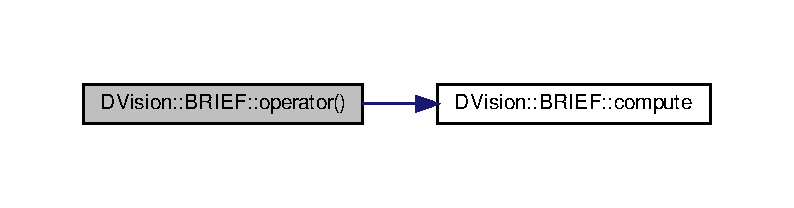
\includegraphics[width=350pt]{classDVision_1_1BRIEF_a290ee93994c09ed3b2164c5d3df182a9_cgraph}
\end{center}
\end{figure}


The documentation for this class was generated from the following files\+:\begin{DoxyCompactItemize}
\item 
pose\+\_\+graph/src/\+Third\+Party/\+D\+Vision/B\+R\+I\+E\+F.\+h\item 
pose\+\_\+graph/src/\+Third\+Party/\+D\+Vision/B\+R\+I\+E\+F.\+cpp\end{DoxyCompactItemize}

\hypertarget{classBriefExtractor}{}\section{Brief\+Extractor Class Reference}
\label{classBriefExtractor}\index{Brief\+Extractor@{Brief\+Extractor}}


Collaboration diagram for Brief\+Extractor\+:\nopagebreak
\begin{figure}[H]
\begin{center}
\leavevmode
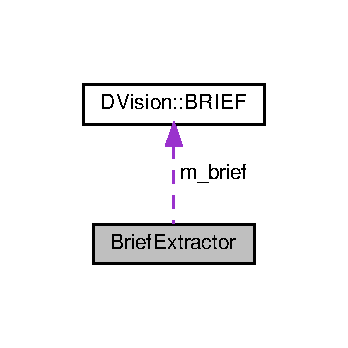
\includegraphics[width=167pt]{classBriefExtractor__coll__graph}
\end{center}
\end{figure}
\subsection*{Public Member Functions}
\begin{DoxyCompactItemize}
\item 
\mbox{\Hypertarget{classBriefExtractor_a435b32055ac9080bf87cd82304e67478}\label{classBriefExtractor_a435b32055ac9080bf87cd82304e67478}} 
virtual void {\bfseries operator()} (const cv\+::\+Mat \&im, vector$<$ cv\+::\+Key\+Point $>$ \&keys, vector$<$ \hyperlink{classDVision_1_1BRIEF_abc56a095174a93b0741099f35230b7c5}{B\+R\+I\+E\+F\+::bitset} $>$ \&descriptors) const
\item 
\mbox{\Hypertarget{classBriefExtractor_a563dde40269338c5518d8bb81c774a41}\label{classBriefExtractor_a563dde40269338c5518d8bb81c774a41}} 
{\bfseries Brief\+Extractor} (const std\+::string \&pattern\+\_\+file)
\end{DoxyCompactItemize}
\subsection*{Public Attributes}
\begin{DoxyCompactItemize}
\item 
\mbox{\Hypertarget{classBriefExtractor_aa30592d6bb3a22172b09376594768387}\label{classBriefExtractor_aa30592d6bb3a22172b09376594768387}} 
\hyperlink{classDVision_1_1BRIEF}{D\+Vision\+::\+B\+R\+I\+EF} {\bfseries m\+\_\+brief}
\end{DoxyCompactItemize}


The documentation for this class was generated from the following files\+:\begin{DoxyCompactItemize}
\item 
pose\+\_\+graph/src/keyframe.\+h\item 
pose\+\_\+graph/src/keyframe.\+cpp\end{DoxyCompactItemize}

\hypertarget{classcamodocal_1_1Camera}{}\section{camodocal\+:\+:Camera Class Reference}
\label{classcamodocal_1_1Camera}\index{camodocal\+::\+Camera@{camodocal\+::\+Camera}}


base class for all camera model  




{\ttfamily \#include $<$Camera.\+h$>$}



Inheritance diagram for camodocal\+:\+:Camera\+:\nopagebreak
\begin{figure}[H]
\begin{center}
\leavevmode
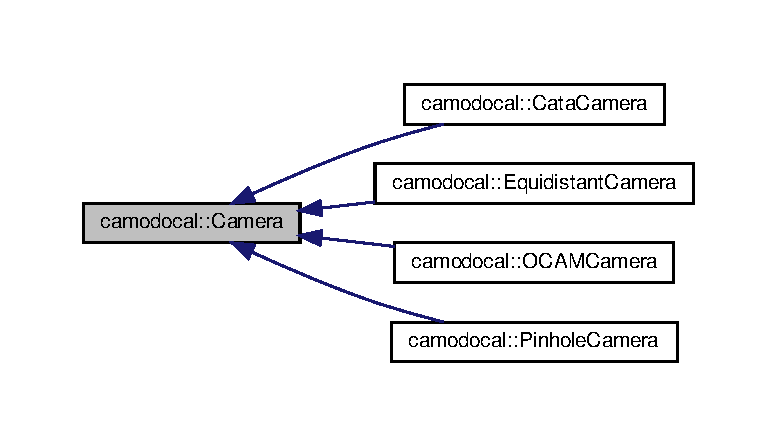
\includegraphics[width=350pt]{classcamodocal_1_1Camera__inherit__graph}
\end{center}
\end{figure}
\subsection*{Classes}
\begin{DoxyCompactItemize}
\item 
class \hyperlink{classcamodocal_1_1Camera_1_1Parameters}{Parameters}
\begin{DoxyCompactList}\small\item\em nested class for camera parameters \end{DoxyCompactList}\end{DoxyCompactItemize}
\subsection*{Public Types}
\begin{DoxyCompactItemize}
\item 
\mbox{\Hypertarget{classcamodocal_1_1Camera_a663bb19b7b1f38f6d1b7eeb0890183ff}\label{classcamodocal_1_1Camera_a663bb19b7b1f38f6d1b7eeb0890183ff}} 
enum \hyperlink{classcamodocal_1_1Camera_a663bb19b7b1f38f6d1b7eeb0890183ff}{Model\+Type} \{ {\bfseries K\+A\+N\+N\+A\+L\+A\+\_\+\+B\+R\+A\+N\+DT}, 
{\bfseries M\+EI}, 
{\bfseries P\+I\+N\+H\+O\+LE}, 
{\bfseries S\+C\+A\+R\+A\+M\+U\+Z\+ZA}
 \}\begin{DoxyCompactList}\small\item\em enumerate variable of camera model \end{DoxyCompactList}
\end{DoxyCompactItemize}
\subsection*{Public Member Functions}
\begin{DoxyCompactItemize}
\item 
\mbox{\Hypertarget{classcamodocal_1_1Camera_aa95c0a2dd8d36b4d5aa7013eb01d1227}\label{classcamodocal_1_1Camera_aa95c0a2dd8d36b4d5aa7013eb01d1227}} 
virtual \hyperlink{classcamodocal_1_1Camera_a663bb19b7b1f38f6d1b7eeb0890183ff}{Model\+Type} \hyperlink{classcamodocal_1_1Camera_aa95c0a2dd8d36b4d5aa7013eb01d1227}{model\+Type} (void) const =0
\begin{DoxyCompactList}\small\item\em virtual type of function model\+Type \end{DoxyCompactList}\item 
\mbox{\Hypertarget{classcamodocal_1_1Camera_ad0a7aafcfd19a6105f3b64f003f0f794}\label{classcamodocal_1_1Camera_ad0a7aafcfd19a6105f3b64f003f0f794}} 
virtual const std\+::string \& \hyperlink{classcamodocal_1_1Camera_ad0a7aafcfd19a6105f3b64f003f0f794}{camera\+Name} (void) const =0
\begin{DoxyCompactList}\small\item\em virtual type of funtion camera\+Name \end{DoxyCompactList}\item 
\mbox{\Hypertarget{classcamodocal_1_1Camera_ad9e799c94b0fddad3f982c30820d7bab}\label{classcamodocal_1_1Camera_ad9e799c94b0fddad3f982c30820d7bab}} 
virtual int \hyperlink{classcamodocal_1_1Camera_ad9e799c94b0fddad3f982c30820d7bab}{image\+Width} (void) const =0
\begin{DoxyCompactList}\small\item\em virtual type of function image\+Width \end{DoxyCompactList}\item 
\mbox{\Hypertarget{classcamodocal_1_1Camera_a2a829050957309327b163e460df32a3d}\label{classcamodocal_1_1Camera_a2a829050957309327b163e460df32a3d}} 
virtual int \hyperlink{classcamodocal_1_1Camera_a2a829050957309327b163e460df32a3d}{image\+Height} (void) const =0
\begin{DoxyCompactList}\small\item\em virtual type of function image\+Height \end{DoxyCompactList}\item 
\mbox{\Hypertarget{classcamodocal_1_1Camera_a1c74aa165487ef4eea0d11ded7946ad1}\label{classcamodocal_1_1Camera_a1c74aa165487ef4eea0d11ded7946ad1}} 
virtual cv\+::\+Mat \& \hyperlink{classcamodocal_1_1Camera_a1c74aa165487ef4eea0d11ded7946ad1}{mask} (void)
\begin{DoxyCompactList}\small\item\em virtual function of image Mask \end{DoxyCompactList}\item 
\mbox{\Hypertarget{classcamodocal_1_1Camera_ab2ef0e5f32fc81f9c568be1234da168b}\label{classcamodocal_1_1Camera_ab2ef0e5f32fc81f9c568be1234da168b}} 
virtual const cv\+::\+Mat \& \hyperlink{classcamodocal_1_1Camera_ab2ef0e5f32fc81f9c568be1234da168b}{mask} (void) const
\begin{DoxyCompactList}\small\item\em virtual function of image Mask \end{DoxyCompactList}\item 
\mbox{\Hypertarget{classcamodocal_1_1Camera_a5b24bfc1b1c88642a99c8ddd8f74d085}\label{classcamodocal_1_1Camera_a5b24bfc1b1c88642a99c8ddd8f74d085}} 
virtual void \hyperlink{classcamodocal_1_1Camera_a5b24bfc1b1c88642a99c8ddd8f74d085}{estimate\+Intrinsics} (const cv\+::\+Size \&board\+Size, const std\+::vector$<$ std\+::vector$<$ cv\+::\+Point3f $>$ $>$ \&object\+Points, const std\+::vector$<$ std\+::vector$<$ cv\+::\+Point2f $>$ $>$ \&image\+Points)=0
\begin{DoxyCompactList}\small\item\em virtual function of camera intrinsics \end{DoxyCompactList}\item 
virtual void \hyperlink{classcamodocal_1_1Camera_a2a6d99ee0927e0336b4d77a9773900a4}{estimate\+Extrinsics} (const std\+::vector$<$ cv\+::\+Point3f $>$ \&object\+Points, const std\+::vector$<$ cv\+::\+Point2f $>$ \&image\+Points, cv\+::\+Mat \&rvec, cv\+::\+Mat \&tvec) const
\begin{DoxyCompactList}\small\item\em calculate extrinsics with unit intrinsics \end{DoxyCompactList}\item 
\mbox{\Hypertarget{classcamodocal_1_1Camera_a77b4ea673c694741302efba6f86a0100}\label{classcamodocal_1_1Camera_a77b4ea673c694741302efba6f86a0100}} 
virtual void \hyperlink{classcamodocal_1_1Camera_a77b4ea673c694741302efba6f86a0100}{lift\+Sphere} (const Eigen\+::\+Vector2d \&p, Eigen\+::\+Vector3d \&P) const =0
\begin{DoxyCompactList}\small\item\em Lift points from the image plane to the sphere. \end{DoxyCompactList}\item 
\mbox{\Hypertarget{classcamodocal_1_1Camera_a680e97bfecab33cd833f914ee811d12d}\label{classcamodocal_1_1Camera_a680e97bfecab33cd833f914ee811d12d}} 
virtual void \hyperlink{classcamodocal_1_1Camera_a680e97bfecab33cd833f914ee811d12d}{lift\+Projective} (const Eigen\+::\+Vector2d \&p, Eigen\+::\+Vector3d \&P) const =0
\begin{DoxyCompactList}\small\item\em Lift points from the image plane to the projective space. \end{DoxyCompactList}\item 
\mbox{\Hypertarget{classcamodocal_1_1Camera_acf49bd1ef0919e0faf89d060dc497b52}\label{classcamodocal_1_1Camera_acf49bd1ef0919e0faf89d060dc497b52}} 
virtual void \hyperlink{classcamodocal_1_1Camera_acf49bd1ef0919e0faf89d060dc497b52}{space\+To\+Plane} (const Eigen\+::\+Vector3d \&P, Eigen\+::\+Vector2d \&p) const =0
\begin{DoxyCompactList}\small\item\em Projects 3D points to the image plane (Pi function) \end{DoxyCompactList}\item 
\mbox{\Hypertarget{classcamodocal_1_1Camera_aa139629842798823cb38dce0019f7a49}\label{classcamodocal_1_1Camera_aa139629842798823cb38dce0019f7a49}} 
virtual void {\bfseries undist\+To\+Plane} (const Eigen\+::\+Vector2d \&p\+\_\+u, Eigen\+::\+Vector2d \&p) const =0
\item 
\mbox{\Hypertarget{classcamodocal_1_1Camera_a79dbf1282a9d4a4dc4a8f1e65cfc657a}\label{classcamodocal_1_1Camera_a79dbf1282a9d4a4dc4a8f1e65cfc657a}} 
virtual cv\+::\+Mat {\bfseries init\+Undistort\+Rectify\+Map} (cv\+::\+Mat \&map1, cv\+::\+Mat \&map2, float fx=-\/1.\+0f, float fy=-\/1.\+0f, cv\+::\+Size image\+Size=cv\+::\+Size(0, 0), float cx=-\/1.\+0f, float cy=-\/1.\+0f, cv\+::\+Mat rmat=cv\+::\+Mat\+::eye(3, 3, C\+V\+\_\+32\+F)) const =0
\item 
\mbox{\Hypertarget{classcamodocal_1_1Camera_a05ed9804daf6803907c716da2581204c}\label{classcamodocal_1_1Camera_a05ed9804daf6803907c716da2581204c}} 
virtual int \hyperlink{classcamodocal_1_1Camera_a05ed9804daf6803907c716da2581204c}{parameter\+Count} (void) const =0
\begin{DoxyCompactList}\small\item\em pure virtual function of parameter count \end{DoxyCompactList}\item 
\mbox{\Hypertarget{classcamodocal_1_1Camera_a40f385799b9ab055cf69b720835ad151}\label{classcamodocal_1_1Camera_a40f385799b9ab055cf69b720835ad151}} 
virtual void \hyperlink{classcamodocal_1_1Camera_a40f385799b9ab055cf69b720835ad151}{read\+Parameters} (const std\+::vector$<$ double $>$ \&parameters)=0
\begin{DoxyCompactList}\small\item\em pure virtual function of reading parameters \end{DoxyCompactList}\item 
\mbox{\Hypertarget{classcamodocal_1_1Camera_afb1d6e23e4918c0dd978ef9d3b57a3e2}\label{classcamodocal_1_1Camera_afb1d6e23e4918c0dd978ef9d3b57a3e2}} 
virtual void \hyperlink{classcamodocal_1_1Camera_afb1d6e23e4918c0dd978ef9d3b57a3e2}{write\+Parameters} (std\+::vector$<$ double $>$ \&parameters) const =0
\begin{DoxyCompactList}\small\item\em pure virtual function of writing parameters \end{DoxyCompactList}\item 
\mbox{\Hypertarget{classcamodocal_1_1Camera_a8dc590b4552c389a079bb64179ac30d7}\label{classcamodocal_1_1Camera_a8dc590b4552c389a079bb64179ac30d7}} 
virtual void \hyperlink{classcamodocal_1_1Camera_a8dc590b4552c389a079bb64179ac30d7}{write\+Parameters\+To\+Yaml\+File} (const std\+::string \&filename) const =0
\begin{DoxyCompactList}\small\item\em pure virtual function of writing parameters to Y\+A\+ML file \end{DoxyCompactList}\item 
\mbox{\Hypertarget{classcamodocal_1_1Camera_a151059e8f00d9a5a9c5db19a128937a6}\label{classcamodocal_1_1Camera_a151059e8f00d9a5a9c5db19a128937a6}} 
virtual std\+::string \hyperlink{classcamodocal_1_1Camera_a151059e8f00d9a5a9c5db19a128937a6}{parameters\+To\+String} (void) const =0
\begin{DoxyCompactList}\small\item\em pure virtual of converting parameters to string \end{DoxyCompactList}\item 
double \hyperlink{classcamodocal_1_1Camera_a544642f8170212af887350cff67d16b5}{reprojection\+Dist} (const Eigen\+::\+Vector3d \&P1, const Eigen\+::\+Vector3d \&P2) const
\begin{DoxyCompactList}\small\item\em Calculates the reprojection distance between points. \end{DoxyCompactList}\item 
double \hyperlink{classcamodocal_1_1Camera_ab162451505d8b9dfda0b96383d597a16}{reprojection\+Error} (const std\+::vector$<$ std\+::vector$<$ cv\+::\+Point3f $>$ $>$ \&object\+Points, const std\+::vector$<$ std\+::vector$<$ cv\+::\+Point2f $>$ $>$ \&image\+Points, const std\+::vector$<$ cv\+::\+Mat $>$ \&rvecs, const std\+::vector$<$ cv\+::\+Mat $>$ \&tvecs, cv\+::\+Output\+Array per\+View\+Errors=cv\+::no\+Array()) const
\begin{DoxyCompactList}\small\item\em calculate average reprojection error of all points in all frames (total error divede by total points) with 3D points and 2D points \end{DoxyCompactList}\item 
double \hyperlink{classcamodocal_1_1Camera_ab261e28c2d056b3149275c01407416a3}{reprojection\+Error} (const Eigen\+::\+Vector3d \&P, const Eigen\+::\+Quaterniond \&camera\+\_\+q, const Eigen\+::\+Vector3d \&camera\+\_\+t, const Eigen\+::\+Vector2d \&observed\+\_\+p) const
\begin{DoxyCompactList}\small\item\em calculate reprojection error of one 3D point with camera pose P \& Q \end{DoxyCompactList}\item 
void \hyperlink{classcamodocal_1_1Camera_ab8dfa1aa8a60c5569920939ba7d85440}{project\+Points} (const std\+::vector$<$ cv\+::\+Point3f $>$ \&object\+Points, const cv\+::\+Mat \&rvec, const cv\+::\+Mat \&tvec, std\+::vector$<$ cv\+::\+Point2f $>$ \&image\+Points) const
\begin{DoxyCompactList}\small\item\em project 3D points to 2d plane \end{DoxyCompactList}\end{DoxyCompactItemize}
\subsection*{Protected Attributes}
\begin{DoxyCompactItemize}
\item 
\mbox{\Hypertarget{classcamodocal_1_1Camera_a3c48cfb66f81f23bbce4cdbc02c64144}\label{classcamodocal_1_1Camera_a3c48cfb66f81f23bbce4cdbc02c64144}} 
cv\+::\+Mat \hyperlink{classcamodocal_1_1Camera_a3c48cfb66f81f23bbce4cdbc02c64144}{m\+\_\+mask}
\begin{DoxyCompactList}\small\item\em image mask \end{DoxyCompactList}\end{DoxyCompactItemize}


\subsection{Detailed Description}
base class for all camera model 

\subsection{Member Function Documentation}
\mbox{\Hypertarget{classcamodocal_1_1Camera_a2a6d99ee0927e0336b4d77a9773900a4}\label{classcamodocal_1_1Camera_a2a6d99ee0927e0336b4d77a9773900a4}} 
\index{camodocal\+::\+Camera@{camodocal\+::\+Camera}!estimate\+Extrinsics@{estimate\+Extrinsics}}
\index{estimate\+Extrinsics@{estimate\+Extrinsics}!camodocal\+::\+Camera@{camodocal\+::\+Camera}}
\subsubsection{\texorpdfstring{estimate\+Extrinsics()}{estimateExtrinsics()}}
{\footnotesize\ttfamily void camodocal\+::\+Camera\+::estimate\+Extrinsics (\begin{DoxyParamCaption}\item[{const std\+::vector$<$ cv\+::\+Point3f $>$ \&}]{object\+Points,  }\item[{const std\+::vector$<$ cv\+::\+Point2f $>$ \&}]{image\+Points,  }\item[{cv\+::\+Mat \&}]{rvec,  }\item[{cv\+::\+Mat \&}]{tvec }\end{DoxyParamCaption}) const\hspace{0.3cm}{\ttfamily [virtual]}}



calculate extrinsics with unit intrinsics 


\begin{DoxyParams}{Parameters}
{\em object\+Points} & 3D points on object \\
\hline
{\em image\+Points} & 2D point on image plane \\
\hline
{\em rvec} & rotation vector \\
\hline
{\em tvec} & transformation vector \\
\hline
\end{DoxyParams}


References lift\+Projective().



Referenced by camodocal\+::\+Cata\+Camera\+::estimate\+Intrinsics(), and camodocal\+::\+Equidistant\+Camera\+::estimate\+Intrinsics().

Here is the call graph for this function\+:\nopagebreak
\begin{figure}[H]
\begin{center}
\leavevmode
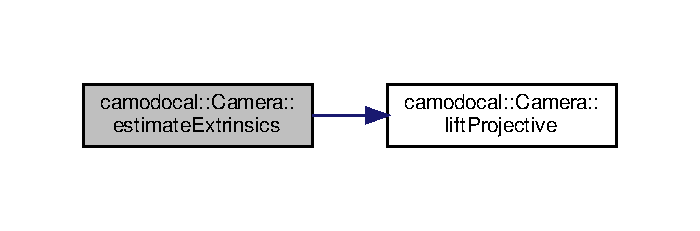
\includegraphics[width=336pt]{classcamodocal_1_1Camera_a2a6d99ee0927e0336b4d77a9773900a4_cgraph}
\end{center}
\end{figure}
Here is the caller graph for this function\+:\nopagebreak
\begin{figure}[H]
\begin{center}
\leavevmode
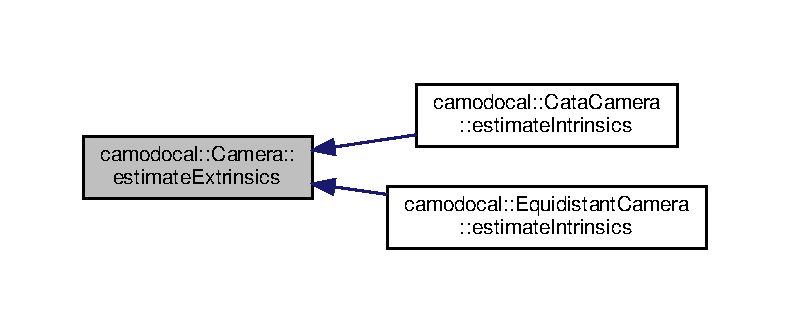
\includegraphics[width=350pt]{classcamodocal_1_1Camera_a2a6d99ee0927e0336b4d77a9773900a4_icgraph}
\end{center}
\end{figure}
\mbox{\Hypertarget{classcamodocal_1_1Camera_ab8dfa1aa8a60c5569920939ba7d85440}\label{classcamodocal_1_1Camera_ab8dfa1aa8a60c5569920939ba7d85440}} 
\index{camodocal\+::\+Camera@{camodocal\+::\+Camera}!project\+Points@{project\+Points}}
\index{project\+Points@{project\+Points}!camodocal\+::\+Camera@{camodocal\+::\+Camera}}
\subsubsection{\texorpdfstring{project\+Points()}{projectPoints()}}
{\footnotesize\ttfamily void camodocal\+::\+Camera\+::project\+Points (\begin{DoxyParamCaption}\item[{const std\+::vector$<$ cv\+::\+Point3f $>$ \&}]{object\+Points,  }\item[{const cv\+::\+Mat \&}]{rvec,  }\item[{const cv\+::\+Mat \&}]{tvec,  }\item[{std\+::vector$<$ cv\+::\+Point2f $>$ \&}]{image\+Points }\end{DoxyParamCaption}) const}



project 3D points to 2d plane 


\begin{DoxyParams}{Parameters}
{\em object\+Points} & \\
\hline
{\em rvec} & \\
\hline
{\em tvec} & \\
\hline
{\em image\+Points} & \\
\hline
\end{DoxyParams}
reserve space for image\+Points according to object\+Points

convert from rotation vector to rotation matrix 

References space\+To\+Plane().



Referenced by reprojection\+Error().

Here is the call graph for this function\+:\nopagebreak
\begin{figure}[H]
\begin{center}
\leavevmode
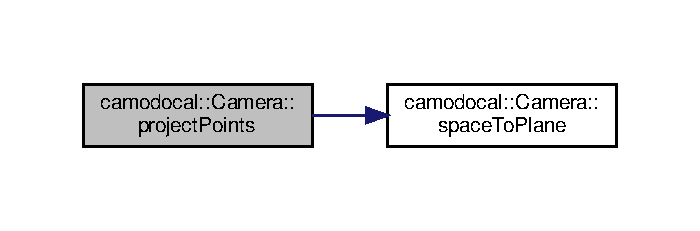
\includegraphics[width=336pt]{classcamodocal_1_1Camera_ab8dfa1aa8a60c5569920939ba7d85440_cgraph}
\end{center}
\end{figure}
Here is the caller graph for this function\+:\nopagebreak
\begin{figure}[H]
\begin{center}
\leavevmode
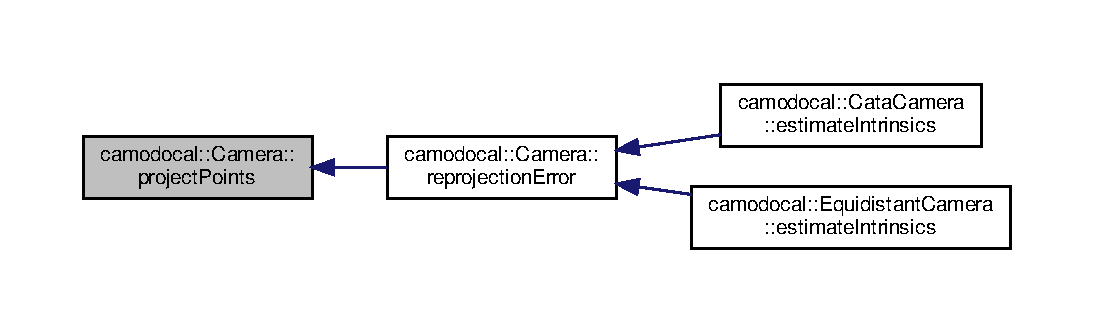
\includegraphics[width=350pt]{classcamodocal_1_1Camera_ab8dfa1aa8a60c5569920939ba7d85440_icgraph}
\end{center}
\end{figure}
\mbox{\Hypertarget{classcamodocal_1_1Camera_a544642f8170212af887350cff67d16b5}\label{classcamodocal_1_1Camera_a544642f8170212af887350cff67d16b5}} 
\index{camodocal\+::\+Camera@{camodocal\+::\+Camera}!reprojection\+Dist@{reprojection\+Dist}}
\index{reprojection\+Dist@{reprojection\+Dist}!camodocal\+::\+Camera@{camodocal\+::\+Camera}}
\subsubsection{\texorpdfstring{reprojection\+Dist()}{reprojectionDist()}}
{\footnotesize\ttfamily double camodocal\+::\+Camera\+::reprojection\+Dist (\begin{DoxyParamCaption}\item[{const Eigen\+::\+Vector3d \&}]{P1,  }\item[{const Eigen\+::\+Vector3d \&}]{P2 }\end{DoxyParamCaption}) const}



Calculates the reprojection distance between points. 


\begin{DoxyParams}{Parameters}
{\em P1} & first 3D point coordinates \\
\hline
{\em P2} & second 3D point coordinates \\
\hline
\end{DoxyParams}
\begin{DoxyReturn}{Returns}
euclidean distance in the plane 
\end{DoxyReturn}


References space\+To\+Plane().

Here is the call graph for this function\+:\nopagebreak
\begin{figure}[H]
\begin{center}
\leavevmode
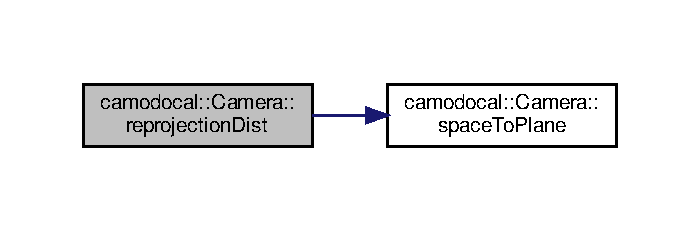
\includegraphics[width=336pt]{classcamodocal_1_1Camera_a544642f8170212af887350cff67d16b5_cgraph}
\end{center}
\end{figure}
\mbox{\Hypertarget{classcamodocal_1_1Camera_ab162451505d8b9dfda0b96383d597a16}\label{classcamodocal_1_1Camera_ab162451505d8b9dfda0b96383d597a16}} 
\index{camodocal\+::\+Camera@{camodocal\+::\+Camera}!reprojection\+Error@{reprojection\+Error}}
\index{reprojection\+Error@{reprojection\+Error}!camodocal\+::\+Camera@{camodocal\+::\+Camera}}
\subsubsection{\texorpdfstring{reprojection\+Error()}{reprojectionError()}\hspace{0.1cm}{\footnotesize\ttfamily [1/2]}}
{\footnotesize\ttfamily double camodocal\+::\+Camera\+::reprojection\+Error (\begin{DoxyParamCaption}\item[{const std\+::vector$<$ std\+::vector$<$ cv\+::\+Point3f $>$ $>$ \&}]{object\+Points,  }\item[{const std\+::vector$<$ std\+::vector$<$ cv\+::\+Point2f $>$ $>$ \&}]{image\+Points,  }\item[{const std\+::vector$<$ cv\+::\+Mat $>$ \&}]{rvecs,  }\item[{const std\+::vector$<$ cv\+::\+Mat $>$ \&}]{tvecs,  }\item[{cv\+::\+Output\+Array}]{per\+View\+Errors = {\ttfamily cv\+:\+:noArray()} }\end{DoxyParamCaption}) const}



calculate average reprojection error of all points in all frames (total error divede by total points) with 3D points and 2D points 


\begin{DoxyParams}{Parameters}
{\em object\+Points} & 3D coordinates of object points \\
\hline
{\em image\+Points} & 2D coordinates of image points \\
\hline
{\em rvecs} & rotation vectors \\
\hline
{\em tvecs} & transformation vectors \\
\hline
{\em per\+View\+Errors} & \\
\hline
\end{DoxyParams}
\begin{DoxyReturn}{Returns}
\+: 
\end{DoxyReturn}
count of image frames

current points in all image frames

check whether pre\+Vire\+Error needed to be computed

image\+Count $\ast$ 1

using get\+Mat() to convert from cv\+::\+Output\+Array to cv\+::\+Mat

project points of frame i to image plane

calculate repeojection error of frame i()

calculate average reprojection error of frame i

return average reprojection error 

References project\+Points().



Referenced by camodocal\+::\+Cata\+Camera\+::estimate\+Intrinsics(), and camodocal\+::\+Equidistant\+Camera\+::estimate\+Intrinsics().

Here is the call graph for this function\+:\nopagebreak
\begin{figure}[H]
\begin{center}
\leavevmode
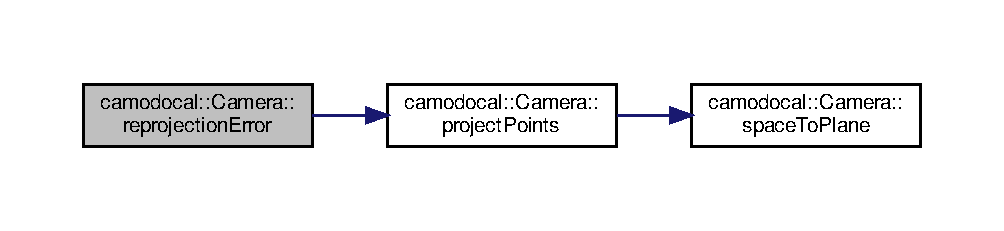
\includegraphics[width=350pt]{classcamodocal_1_1Camera_ab162451505d8b9dfda0b96383d597a16_cgraph}
\end{center}
\end{figure}
Here is the caller graph for this function\+:\nopagebreak
\begin{figure}[H]
\begin{center}
\leavevmode
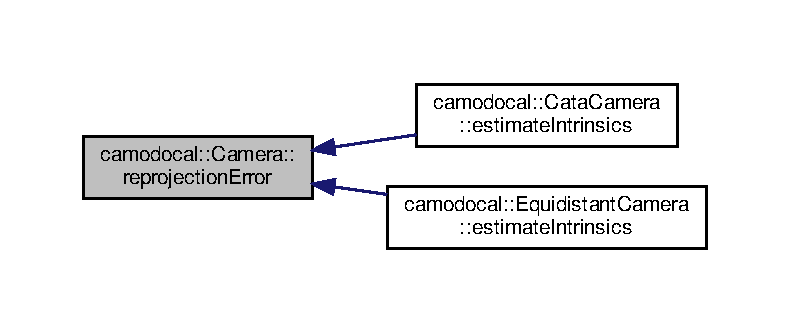
\includegraphics[width=350pt]{classcamodocal_1_1Camera_ab162451505d8b9dfda0b96383d597a16_icgraph}
\end{center}
\end{figure}
\mbox{\Hypertarget{classcamodocal_1_1Camera_ab261e28c2d056b3149275c01407416a3}\label{classcamodocal_1_1Camera_ab261e28c2d056b3149275c01407416a3}} 
\index{camodocal\+::\+Camera@{camodocal\+::\+Camera}!reprojection\+Error@{reprojection\+Error}}
\index{reprojection\+Error@{reprojection\+Error}!camodocal\+::\+Camera@{camodocal\+::\+Camera}}
\subsubsection{\texorpdfstring{reprojection\+Error()}{reprojectionError()}\hspace{0.1cm}{\footnotesize\ttfamily [2/2]}}
{\footnotesize\ttfamily double camodocal\+::\+Camera\+::reprojection\+Error (\begin{DoxyParamCaption}\item[{const Eigen\+::\+Vector3d \&}]{P,  }\item[{const Eigen\+::\+Quaterniond \&}]{camera\+\_\+q,  }\item[{const Eigen\+::\+Vector3d \&}]{camera\+\_\+t,  }\item[{const Eigen\+::\+Vector2d \&}]{observed\+\_\+p }\end{DoxyParamCaption}) const}



calculate reprojection error of one 3D point with camera pose P \& Q 


\begin{DoxyParams}{Parameters}
{\em P} & 3D coordinates of point \\
\hline
{\em camera\+\_\+q} & quaternion of camera pose \\
\hline
{\em camera\+\_\+t} & translation of camera pose \\
\hline
{\em observed\+\_\+p} & corresponding image point \\
\hline
\end{DoxyParams}
\begin{DoxyReturn}{Returns}
\+: 
\end{DoxyReturn}


References space\+To\+Plane().

Here is the call graph for this function\+:\nopagebreak
\begin{figure}[H]
\begin{center}
\leavevmode
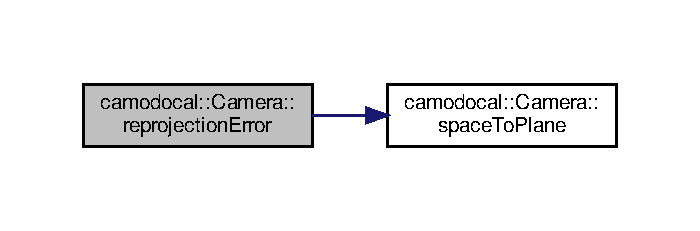
\includegraphics[width=336pt]{classcamodocal_1_1Camera_ab261e28c2d056b3149275c01407416a3_cgraph}
\end{center}
\end{figure}


The documentation for this class was generated from the following files\+:\begin{DoxyCompactItemize}
\item 
camera\+\_\+model/include/camodocal/camera\+\_\+models/\hyperlink{Camera_8h}{Camera.\+h}\item 
camera\+\_\+model/src/camera\+\_\+models/\hyperlink{Camera_8cc}{Camera.\+cc}\end{DoxyCompactItemize}

\hypertarget{classcamodocal_1_1CameraCalibration}{}\section{camodocal\+:\+:Camera\+Calibration Class Reference}
\label{classcamodocal_1_1CameraCalibration}\index{camodocal\+::\+Camera\+Calibration@{camodocal\+::\+Camera\+Calibration}}
\subsection*{Public Member Functions}
\begin{DoxyCompactItemize}
\item 
\mbox{\Hypertarget{classcamodocal_1_1CameraCalibration_aeadd443792485a4d6590ea02e4ce3557}\label{classcamodocal_1_1CameraCalibration_aeadd443792485a4d6590ea02e4ce3557}} 
{\bfseries Camera\+Calibration} (\hyperlink{classcamodocal_1_1Camera_a663bb19b7b1f38f6d1b7eeb0890183ff}{Camera\+::\+Model\+Type} model\+Type, const std\+::string \&camera\+Name, const cv\+::\+Size \&image\+Size, const cv\+::\+Size \&board\+Size, float square\+Size)
\item 
\mbox{\Hypertarget{classcamodocal_1_1CameraCalibration_a07e5e523c16159536c92cade483a64bd}\label{classcamodocal_1_1CameraCalibration_a07e5e523c16159536c92cade483a64bd}} 
void {\bfseries clear} (void)
\item 
\mbox{\Hypertarget{classcamodocal_1_1CameraCalibration_a41ab885dc75b4c23e8bef62af89573b2}\label{classcamodocal_1_1CameraCalibration_a41ab885dc75b4c23e8bef62af89573b2}} 
void {\bfseries add\+Chessboard\+Data} (const std\+::vector$<$ cv\+::\+Point2f $>$ \&corners)
\item 
\mbox{\Hypertarget{classcamodocal_1_1CameraCalibration_af0638fb51c1e633814403a6be89f45fe}\label{classcamodocal_1_1CameraCalibration_af0638fb51c1e633814403a6be89f45fe}} 
bool {\bfseries calibrate} (void)
\item 
\mbox{\Hypertarget{classcamodocal_1_1CameraCalibration_ab840e8335fc0e281b75269a14321c2df}\label{classcamodocal_1_1CameraCalibration_ab840e8335fc0e281b75269a14321c2df}} 
int {\bfseries sample\+Count} (void) const
\item 
\mbox{\Hypertarget{classcamodocal_1_1CameraCalibration_a1559248803a3d8fe4bfefb34d209e77e}\label{classcamodocal_1_1CameraCalibration_a1559248803a3d8fe4bfefb34d209e77e}} 
std\+::vector$<$ std\+::vector$<$ cv\+::\+Point2f $>$ $>$ \& {\bfseries image\+Points} (void)
\item 
\mbox{\Hypertarget{classcamodocal_1_1CameraCalibration_a7b89b69c893486fda5f3f0cd75c1d053}\label{classcamodocal_1_1CameraCalibration_a7b89b69c893486fda5f3f0cd75c1d053}} 
const std\+::vector$<$ std\+::vector$<$ cv\+::\+Point2f $>$ $>$ \& {\bfseries image\+Points} (void) const
\item 
\mbox{\Hypertarget{classcamodocal_1_1CameraCalibration_a6f850b6c713b5a822a0b6e4310017a0c}\label{classcamodocal_1_1CameraCalibration_a6f850b6c713b5a822a0b6e4310017a0c}} 
std\+::vector$<$ std\+::vector$<$ cv\+::\+Point3f $>$ $>$ \& {\bfseries scene\+Points} (void)
\item 
\mbox{\Hypertarget{classcamodocal_1_1CameraCalibration_a34f423299c758173cf2fd2ec5080fd42}\label{classcamodocal_1_1CameraCalibration_a34f423299c758173cf2fd2ec5080fd42}} 
const std\+::vector$<$ std\+::vector$<$ cv\+::\+Point3f $>$ $>$ \& {\bfseries scene\+Points} (void) const
\item 
\mbox{\Hypertarget{classcamodocal_1_1CameraCalibration_a36314a8ff7d13853ec2fa572f6230588}\label{classcamodocal_1_1CameraCalibration_a36314a8ff7d13853ec2fa572f6230588}} 
\hyperlink{Camera_8h_a9f66c7d396fa23ffb2a4512670a78b84}{Camera\+Ptr} \& {\bfseries camera} (void)
\item 
\mbox{\Hypertarget{classcamodocal_1_1CameraCalibration_ad0851d9b65acfe775d75d5973b5f754a}\label{classcamodocal_1_1CameraCalibration_ad0851d9b65acfe775d75d5973b5f754a}} 
const \hyperlink{Camera_8h_a03fe5d6885a007cb4ad26d11f6198586}{Camera\+Const\+Ptr} {\bfseries camera} (void) const
\item 
\mbox{\Hypertarget{classcamodocal_1_1CameraCalibration_a45df9fe3fa2cf4ab9d3002eb0636bb72}\label{classcamodocal_1_1CameraCalibration_a45df9fe3fa2cf4ab9d3002eb0636bb72}} 
Eigen\+::\+Matrix2d \& {\bfseries measurement\+Covariance} (void)
\item 
\mbox{\Hypertarget{classcamodocal_1_1CameraCalibration_a8fe3e53a6ad83a0c28d196ae6114014c}\label{classcamodocal_1_1CameraCalibration_a8fe3e53a6ad83a0c28d196ae6114014c}} 
const Eigen\+::\+Matrix2d \& {\bfseries measurement\+Covariance} (void) const
\item 
\mbox{\Hypertarget{classcamodocal_1_1CameraCalibration_afaa75cf84619b2660e0e2adb1ec7f7d0}\label{classcamodocal_1_1CameraCalibration_afaa75cf84619b2660e0e2adb1ec7f7d0}} 
cv\+::\+Mat \& {\bfseries camera\+Poses} (void)
\item 
\mbox{\Hypertarget{classcamodocal_1_1CameraCalibration_a5406b15c8ce833a38c960cb54b405c1c}\label{classcamodocal_1_1CameraCalibration_a5406b15c8ce833a38c960cb54b405c1c}} 
const cv\+::\+Mat \& {\bfseries camera\+Poses} (void) const
\item 
\mbox{\Hypertarget{classcamodocal_1_1CameraCalibration_af6da01f9e5aab14beabbbec5bb3c4e69}\label{classcamodocal_1_1CameraCalibration_af6da01f9e5aab14beabbbec5bb3c4e69}} 
void {\bfseries draw\+Results} (std\+::vector$<$ cv\+::\+Mat $>$ \&images) const
\item 
\mbox{\Hypertarget{classcamodocal_1_1CameraCalibration_a65a11eafa17db001f81daa1440f25ae2}\label{classcamodocal_1_1CameraCalibration_a65a11eafa17db001f81daa1440f25ae2}} 
void {\bfseries write\+Params} (const std\+::string \&filename) const
\item 
\mbox{\Hypertarget{classcamodocal_1_1CameraCalibration_af4d5a4fb78fb44fa7486b97cce5a9ddb}\label{classcamodocal_1_1CameraCalibration_af4d5a4fb78fb44fa7486b97cce5a9ddb}} 
bool {\bfseries write\+Chessboard\+Data} (const std\+::string \&filename) const
\item 
\mbox{\Hypertarget{classcamodocal_1_1CameraCalibration_a32e882640042a6684d0b772c4f27c977}\label{classcamodocal_1_1CameraCalibration_a32e882640042a6684d0b772c4f27c977}} 
bool {\bfseries read\+Chessboard\+Data} (const std\+::string \&filename)
\item 
\mbox{\Hypertarget{classcamodocal_1_1CameraCalibration_add7f51ba49bc48088568377259cc7201}\label{classcamodocal_1_1CameraCalibration_add7f51ba49bc48088568377259cc7201}} 
void {\bfseries set\+Verbose} (bool verbose)
\end{DoxyCompactItemize}


The documentation for this class was generated from the following files\+:\begin{DoxyCompactItemize}
\item 
camera\+\_\+model/include/camodocal/calib/Camera\+Calibration.\+h\item 
camera\+\_\+model/src/calib/Camera\+Calibration.\+cc\end{DoxyCompactItemize}

\hypertarget{classcamodocal_1_1CameraFactory}{}\section{camodocal\+:\+:Camera\+Factory Class Reference}
\label{classcamodocal_1_1CameraFactory}\index{camodocal\+::\+Camera\+Factory@{camodocal\+::\+Camera\+Factory}}
\subsection*{Public Member Functions}
\begin{DoxyCompactItemize}
\item 
\hyperlink{Camera_8h_a9f66c7d396fa23ffb2a4512670a78b84}{Camera\+Ptr} \hyperlink{classcamodocal_1_1CameraFactory_a853fe9e847faae5caa3981f87a9ab7c8}{generate\+Camera} (\hyperlink{classcamodocal_1_1Camera_a663bb19b7b1f38f6d1b7eeb0890183ff}{Camera\+::\+Model\+Type} model\+Type, const std\+::string \&camera\+Name, cv\+::\+Size image\+Size) const
\begin{DoxyCompactList}\small\item\em generate \hyperlink{classcamodocal_1_1Camera}{Camera} object according to model\+Type \end{DoxyCompactList}\item 
\hyperlink{Camera_8h_a9f66c7d396fa23ffb2a4512670a78b84}{Camera\+Ptr} \hyperlink{classcamodocal_1_1CameraFactory_a8362492960d68a4ae43c40a1952df3a5}{generate\+Camera\+From\+Yaml\+File} (const std\+::string \&filename)
\begin{DoxyCompactList}\small\item\em generate camera object according to Y\+A\+ML file \end{DoxyCompactList}\end{DoxyCompactItemize}
\subsection*{Static Public Member Functions}
\begin{DoxyCompactItemize}
\item 
static boost\+::shared\+\_\+ptr$<$ \hyperlink{classcamodocal_1_1CameraFactory}{Camera\+Factory} $>$ \hyperlink{classcamodocal_1_1CameraFactory_a64645e95b821303ea4b550cb18f2641c}{instance} (void)
\begin{DoxyCompactList}\small\item\em Get point of camera\+Factory. \end{DoxyCompactList}\end{DoxyCompactItemize}


\subsection{Member Function Documentation}
\mbox{\Hypertarget{classcamodocal_1_1CameraFactory_a853fe9e847faae5caa3981f87a9ab7c8}\label{classcamodocal_1_1CameraFactory_a853fe9e847faae5caa3981f87a9ab7c8}} 
\index{camodocal\+::\+Camera\+Factory@{camodocal\+::\+Camera\+Factory}!generate\+Camera@{generate\+Camera}}
\index{generate\+Camera@{generate\+Camera}!camodocal\+::\+Camera\+Factory@{camodocal\+::\+Camera\+Factory}}
\subsubsection{\texorpdfstring{generate\+Camera()}{generateCamera()}}
{\footnotesize\ttfamily \hyperlink{Camera_8h_a9f66c7d396fa23ffb2a4512670a78b84}{Camera\+Ptr} camodocal\+::\+Camera\+Factory\+::generate\+Camera (\begin{DoxyParamCaption}\item[{\hyperlink{classcamodocal_1_1Camera_a663bb19b7b1f38f6d1b7eeb0890183ff}{Camera\+::\+Model\+Type}}]{model\+Type,  }\item[{const std\+::string \&}]{camera\+Name,  }\item[{cv\+::\+Size}]{image\+Size }\end{DoxyParamCaption}) const}



generate \hyperlink{classcamodocal_1_1Camera}{Camera} object according to model\+Type 


\begin{DoxyParams}{Parameters}
{\em model\+Type} & camera model \\
\hline
{\em camera\+Name} & camera name \\
\hline
{\em image\+Size} & image Size \\
\hline
\end{DoxyParams}
\begin{DoxyReturn}{Returns}
\+: shared\+\_\+ptr of camera 
\end{DoxyReturn}


References camodocal\+::\+Camera\+::\+Parameters\+::camera\+Name(), camodocal\+::\+Camera\+::\+Parameters\+::image\+Height(), and camodocal\+::\+Camera\+::\+Parameters\+::image\+Width().

Here is the call graph for this function\+:\nopagebreak
\begin{figure}[H]
\begin{center}
\leavevmode
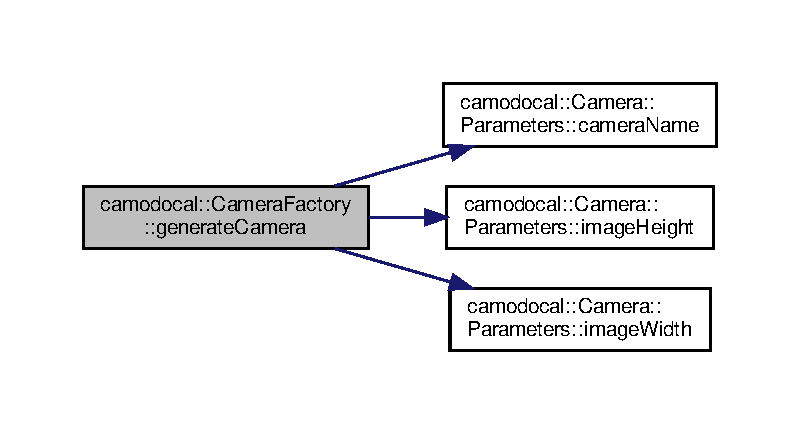
\includegraphics[width=350pt]{classcamodocal_1_1CameraFactory_a853fe9e847faae5caa3981f87a9ab7c8_cgraph}
\end{center}
\end{figure}
\mbox{\Hypertarget{classcamodocal_1_1CameraFactory_a8362492960d68a4ae43c40a1952df3a5}\label{classcamodocal_1_1CameraFactory_a8362492960d68a4ae43c40a1952df3a5}} 
\index{camodocal\+::\+Camera\+Factory@{camodocal\+::\+Camera\+Factory}!generate\+Camera\+From\+Yaml\+File@{generate\+Camera\+From\+Yaml\+File}}
\index{generate\+Camera\+From\+Yaml\+File@{generate\+Camera\+From\+Yaml\+File}!camodocal\+::\+Camera\+Factory@{camodocal\+::\+Camera\+Factory}}
\subsubsection{\texorpdfstring{generate\+Camera\+From\+Yaml\+File()}{generateCameraFromYamlFile()}}
{\footnotesize\ttfamily \hyperlink{Camera_8h_a9f66c7d396fa23ffb2a4512670a78b84}{Camera\+Ptr} camodocal\+::\+Camera\+Factory\+::generate\+Camera\+From\+Yaml\+File (\begin{DoxyParamCaption}\item[{const std\+::string \&}]{filename }\end{DoxyParamCaption})}



generate camera object according to Y\+A\+ML file 


\begin{DoxyParams}{Parameters}
{\em filename} & name of Y\+A\+ML file \\
\hline
\end{DoxyParams}
\begin{DoxyReturn}{Returns}
\+: shared\+\_\+ptr of camera 
\end{DoxyReturn}


References camodocal\+::\+Pinhole\+Camera\+::\+Parameters\+::read\+From\+Yaml\+File(), camodocal\+::\+Equidistant\+Camera\+::\+Parameters\+::read\+From\+Yaml\+File(), camodocal\+::\+O\+C\+A\+M\+Camera\+::\+Parameters\+::read\+From\+Yaml\+File(), and camodocal\+::\+Cata\+Camera\+::\+Parameters\+::read\+From\+Yaml\+File().

Here is the call graph for this function\+:\nopagebreak
\begin{figure}[H]
\begin{center}
\leavevmode
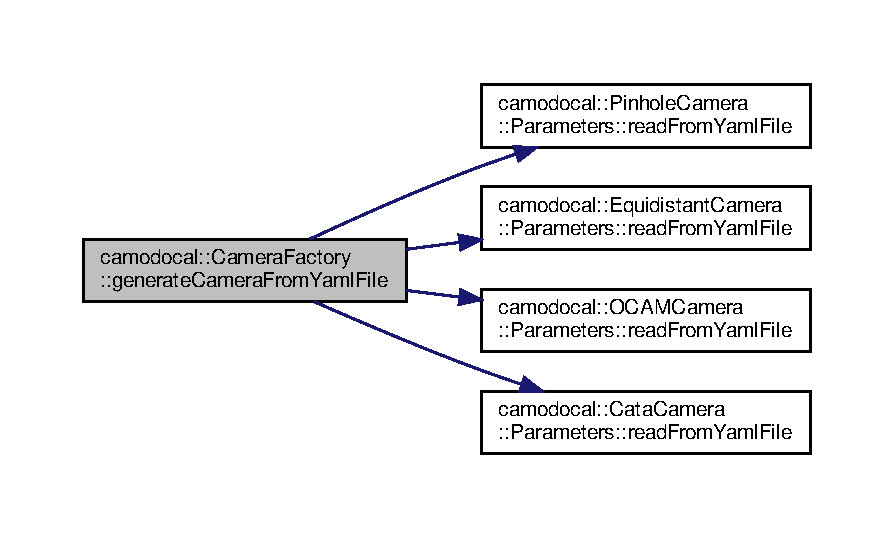
\includegraphics[width=350pt]{classcamodocal_1_1CameraFactory_a8362492960d68a4ae43c40a1952df3a5_cgraph}
\end{center}
\end{figure}
\mbox{\Hypertarget{classcamodocal_1_1CameraFactory_a64645e95b821303ea4b550cb18f2641c}\label{classcamodocal_1_1CameraFactory_a64645e95b821303ea4b550cb18f2641c}} 
\index{camodocal\+::\+Camera\+Factory@{camodocal\+::\+Camera\+Factory}!instance@{instance}}
\index{instance@{instance}!camodocal\+::\+Camera\+Factory@{camodocal\+::\+Camera\+Factory}}
\subsubsection{\texorpdfstring{instance()}{instance()}}
{\footnotesize\ttfamily boost\+::shared\+\_\+ptr$<$ \hyperlink{classcamodocal_1_1CameraFactory}{Camera\+Factory} $>$ camodocal\+::\+Camera\+Factory\+::instance (\begin{DoxyParamCaption}\item[{void}]{ }\end{DoxyParamCaption})\hspace{0.3cm}{\ttfamily [static]}}



Get point of camera\+Factory. 

\begin{DoxyReturn}{Returns}
\+: shared\+\_\+ptr of \hyperlink{classcamodocal_1_1CameraFactory}{Camera\+Factory} 
\end{DoxyReturn}


The documentation for this class was generated from the following files\+:\begin{DoxyCompactItemize}
\item 
camera\+\_\+model/include/camodocal/camera\+\_\+models/Camera\+Factory.\+h\item 
camera\+\_\+model/src/camera\+\_\+models/Camera\+Factory.\+cc\end{DoxyCompactItemize}

\hypertarget{classCameraPoseVisualization}{}\section{Camera\+Pose\+Visualization Class Reference}
\label{classCameraPoseVisualization}\index{Camera\+Pose\+Visualization@{Camera\+Pose\+Visualization}}
\subsection*{Public Member Functions}
\begin{DoxyCompactItemize}
\item 
\mbox{\Hypertarget{classCameraPoseVisualization_ab0900a96947ea4a31603c99253d3e8a2}\label{classCameraPoseVisualization_ab0900a96947ea4a31603c99253d3e8a2}} 
{\bfseries Camera\+Pose\+Visualization} (float r, float g, float b, float a)
\item 
\mbox{\Hypertarget{classCameraPoseVisualization_ad0077b4ae7856a219648e698b0e19583}\label{classCameraPoseVisualization_ad0077b4ae7856a219648e698b0e19583}} 
void {\bfseries set\+Image\+Boundary\+Color} (float r, float g, float b, float a=1.\+0)
\item 
\mbox{\Hypertarget{classCameraPoseVisualization_a97ba9b67388cbec777ba699cb9b16b60}\label{classCameraPoseVisualization_a97ba9b67388cbec777ba699cb9b16b60}} 
void {\bfseries set\+Optical\+Center\+Connector\+Color} (float r, float g, float b, float a=1.\+0)
\item 
\mbox{\Hypertarget{classCameraPoseVisualization_ad80a8caac209f5c8152a11d76a7bdb13}\label{classCameraPoseVisualization_ad80a8caac209f5c8152a11d76a7bdb13}} 
void {\bfseries set\+Scale} (double s)
\item 
\mbox{\Hypertarget{classCameraPoseVisualization_aaff71a7169d94c3430b2720be940e34f}\label{classCameraPoseVisualization_aaff71a7169d94c3430b2720be940e34f}} 
void {\bfseries set\+Line\+Width} (double width)
\item 
\mbox{\Hypertarget{classCameraPoseVisualization_acd8c3319206d898250db48154bd4712b}\label{classCameraPoseVisualization_acd8c3319206d898250db48154bd4712b}} 
void {\bfseries add\+\_\+pose} (const Eigen\+::\+Vector3d \&p, const Eigen\+::\+Quaterniond \&q)
\item 
\mbox{\Hypertarget{classCameraPoseVisualization_a0a6a3843b6c43675ee8d3862b274394a}\label{classCameraPoseVisualization_a0a6a3843b6c43675ee8d3862b274394a}} 
void {\bfseries reset} ()
\item 
\mbox{\Hypertarget{classCameraPoseVisualization_af622cbb53e629b09a19dcd0396ce0c1d}\label{classCameraPoseVisualization_af622cbb53e629b09a19dcd0396ce0c1d}} 
void {\bfseries publish\+\_\+by} (ros\+::\+Publisher \&pub, const std\+\_\+msgs\+::\+Header \&header)
\item 
\mbox{\Hypertarget{classCameraPoseVisualization_a2e3e88742eff639180ba89e2f25ee04f}\label{classCameraPoseVisualization_a2e3e88742eff639180ba89e2f25ee04f}} 
void {\bfseries add\+\_\+edge} (const Eigen\+::\+Vector3d \&p0, const Eigen\+::\+Vector3d \&p1)
\item 
\mbox{\Hypertarget{classCameraPoseVisualization_a632e29693827194f8d16afb426992bce}\label{classCameraPoseVisualization_a632e29693827194f8d16afb426992bce}} 
void {\bfseries add\+\_\+loopedge} (const Eigen\+::\+Vector3d \&p0, const Eigen\+::\+Vector3d \&p1)
\item 
\mbox{\Hypertarget{classCameraPoseVisualization_a0ee421fa2b43cba8addbe508a7c6c8d1}\label{classCameraPoseVisualization_a0ee421fa2b43cba8addbe508a7c6c8d1}} 
void {\bfseries publish\+\_\+image\+\_\+by} (ros\+::\+Publisher \&pub, const std\+\_\+msgs\+::\+Header \&header)
\item 
\mbox{\Hypertarget{classCameraPoseVisualization_ab0900a96947ea4a31603c99253d3e8a2}\label{classCameraPoseVisualization_ab0900a96947ea4a31603c99253d3e8a2}} 
{\bfseries Camera\+Pose\+Visualization} (float r, float g, float b, float a)
\item 
\mbox{\Hypertarget{classCameraPoseVisualization_ad0077b4ae7856a219648e698b0e19583}\label{classCameraPoseVisualization_ad0077b4ae7856a219648e698b0e19583}} 
void {\bfseries set\+Image\+Boundary\+Color} (float r, float g, float b, float a=1.\+0)
\item 
\mbox{\Hypertarget{classCameraPoseVisualization_a97ba9b67388cbec777ba699cb9b16b60}\label{classCameraPoseVisualization_a97ba9b67388cbec777ba699cb9b16b60}} 
void {\bfseries set\+Optical\+Center\+Connector\+Color} (float r, float g, float b, float a=1.\+0)
\item 
\mbox{\Hypertarget{classCameraPoseVisualization_ad80a8caac209f5c8152a11d76a7bdb13}\label{classCameraPoseVisualization_ad80a8caac209f5c8152a11d76a7bdb13}} 
void {\bfseries set\+Scale} (double s)
\item 
\mbox{\Hypertarget{classCameraPoseVisualization_aaff71a7169d94c3430b2720be940e34f}\label{classCameraPoseVisualization_aaff71a7169d94c3430b2720be940e34f}} 
void {\bfseries set\+Line\+Width} (double width)
\item 
\mbox{\Hypertarget{classCameraPoseVisualization_acd8c3319206d898250db48154bd4712b}\label{classCameraPoseVisualization_acd8c3319206d898250db48154bd4712b}} 
void {\bfseries add\+\_\+pose} (const Eigen\+::\+Vector3d \&p, const Eigen\+::\+Quaterniond \&q)
\item 
\mbox{\Hypertarget{classCameraPoseVisualization_a0a6a3843b6c43675ee8d3862b274394a}\label{classCameraPoseVisualization_a0a6a3843b6c43675ee8d3862b274394a}} 
void {\bfseries reset} ()
\item 
\mbox{\Hypertarget{classCameraPoseVisualization_af622cbb53e629b09a19dcd0396ce0c1d}\label{classCameraPoseVisualization_af622cbb53e629b09a19dcd0396ce0c1d}} 
void {\bfseries publish\+\_\+by} (ros\+::\+Publisher \&pub, const std\+\_\+msgs\+::\+Header \&header)
\item 
\mbox{\Hypertarget{classCameraPoseVisualization_a2e3e88742eff639180ba89e2f25ee04f}\label{classCameraPoseVisualization_a2e3e88742eff639180ba89e2f25ee04f}} 
void {\bfseries add\+\_\+edge} (const Eigen\+::\+Vector3d \&p0, const Eigen\+::\+Vector3d \&p1)
\item 
\mbox{\Hypertarget{classCameraPoseVisualization_a632e29693827194f8d16afb426992bce}\label{classCameraPoseVisualization_a632e29693827194f8d16afb426992bce}} 
void {\bfseries add\+\_\+loopedge} (const Eigen\+::\+Vector3d \&p0, const Eigen\+::\+Vector3d \&p1)
\end{DoxyCompactItemize}
\subsection*{Public Attributes}
\begin{DoxyCompactItemize}
\item 
\mbox{\Hypertarget{classCameraPoseVisualization_ab763ec726c4104cfc3f76eb9ba91bc1c}\label{classCameraPoseVisualization_ab763ec726c4104cfc3f76eb9ba91bc1c}} 
std\+::string {\bfseries m\+\_\+marker\+\_\+ns}
\end{DoxyCompactItemize}


The documentation for this class was generated from the following files\+:\begin{DoxyCompactItemize}
\item 
pose\+\_\+graph/src/utility/Camera\+Pose\+Visualization.\+h\item 
pose\+\_\+graph/src/utility/Camera\+Pose\+Visualization.\+cpp\end{DoxyCompactItemize}

\hypertarget{classcamodocal_1_1CataCamera}{}\section{camodocal\+:\+:Cata\+Camera Class Reference}
\label{classcamodocal_1_1CataCamera}\index{camodocal\+::\+Cata\+Camera@{camodocal\+::\+Cata\+Camera}}


{\ttfamily \#include $<$Cata\+Camera.\+h$>$}



Inheritance diagram for camodocal\+:\+:Cata\+Camera\+:\nopagebreak
\begin{figure}[H]
\begin{center}
\leavevmode
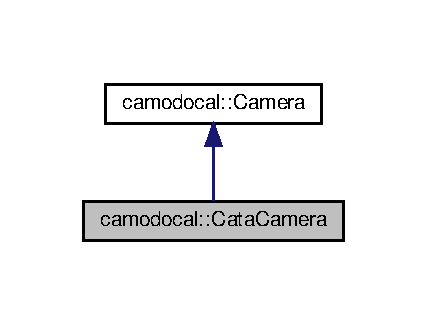
\includegraphics[width=205pt]{classcamodocal_1_1CataCamera__inherit__graph}
\end{center}
\end{figure}


Collaboration diagram for camodocal\+:\+:Cata\+Camera\+:\nopagebreak
\begin{figure}[H]
\begin{center}
\leavevmode
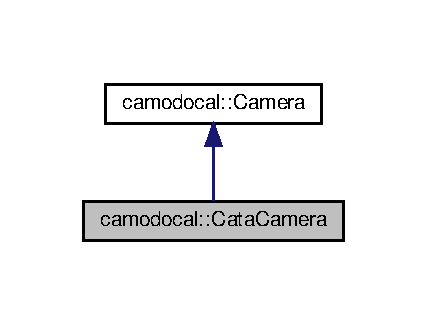
\includegraphics[width=205pt]{classcamodocal_1_1CataCamera__coll__graph}
\end{center}
\end{figure}
\subsection*{Classes}
\begin{DoxyCompactItemize}
\item 
class \hyperlink{classcamodocal_1_1CataCamera_1_1Parameters}{Parameters}
\end{DoxyCompactItemize}
\subsection*{Public Member Functions}
\begin{DoxyCompactItemize}
\item 
\mbox{\Hypertarget{classcamodocal_1_1CataCamera_a648e788b11ea6037f95e3d7fb52c319b}\label{classcamodocal_1_1CataCamera_a648e788b11ea6037f95e3d7fb52c319b}} 
\hyperlink{classcamodocal_1_1CataCamera_a648e788b11ea6037f95e3d7fb52c319b}{Cata\+Camera} (const std\+::string \&\hyperlink{classcamodocal_1_1CataCamera_a0d7729df53b75f8c616a8fc43b7aba13}{camera\+Name}, int \hyperlink{classcamodocal_1_1CataCamera_a12efd82807e3f3baa13c3d5e344ac6a4}{image\+Width}, int \hyperlink{classcamodocal_1_1CataCamera_a858e474daed69f8bbe3aa6d6a1e7d3cc}{image\+Height}, double xi, double k1, double k2, double p1, double p2, double gamma1, double gamma2, double u0, double v0)
\begin{DoxyCompactList}\small\item\em Constructor from the projection model parameters. \end{DoxyCompactList}\item 
\mbox{\Hypertarget{classcamodocal_1_1CataCamera_aa5b09599be0386cf19099b11e23e51eb}\label{classcamodocal_1_1CataCamera_aa5b09599be0386cf19099b11e23e51eb}} 
\hyperlink{classcamodocal_1_1CataCamera_aa5b09599be0386cf19099b11e23e51eb}{Cata\+Camera} (const \hyperlink{classcamodocal_1_1CataCamera_1_1Parameters}{Parameters} \&params)
\begin{DoxyCompactList}\small\item\em Constructor from the projection model parameters. \end{DoxyCompactList}\item 
\mbox{\Hypertarget{classcamodocal_1_1CataCamera_a35b52f562558905b13f51a2a5879ebb1}\label{classcamodocal_1_1CataCamera_a35b52f562558905b13f51a2a5879ebb1}} 
\hyperlink{classcamodocal_1_1Camera_a663bb19b7b1f38f6d1b7eeb0890183ff}{Camera\+::\+Model\+Type} \hyperlink{classcamodocal_1_1CataCamera_a35b52f562558905b13f51a2a5879ebb1}{model\+Type} (void) const
\begin{DoxyCompactList}\small\item\em virtual type of function model\+Type \end{DoxyCompactList}\item 
\mbox{\Hypertarget{classcamodocal_1_1CataCamera_a0d7729df53b75f8c616a8fc43b7aba13}\label{classcamodocal_1_1CataCamera_a0d7729df53b75f8c616a8fc43b7aba13}} 
const std\+::string \& \hyperlink{classcamodocal_1_1CataCamera_a0d7729df53b75f8c616a8fc43b7aba13}{camera\+Name} (void) const
\begin{DoxyCompactList}\small\item\em virtual type of funtion camera\+Name \end{DoxyCompactList}\item 
\mbox{\Hypertarget{classcamodocal_1_1CataCamera_a12efd82807e3f3baa13c3d5e344ac6a4}\label{classcamodocal_1_1CataCamera_a12efd82807e3f3baa13c3d5e344ac6a4}} 
int \hyperlink{classcamodocal_1_1CataCamera_a12efd82807e3f3baa13c3d5e344ac6a4}{image\+Width} (void) const
\begin{DoxyCompactList}\small\item\em virtual type of function image\+Width \end{DoxyCompactList}\item 
\mbox{\Hypertarget{classcamodocal_1_1CataCamera_a858e474daed69f8bbe3aa6d6a1e7d3cc}\label{classcamodocal_1_1CataCamera_a858e474daed69f8bbe3aa6d6a1e7d3cc}} 
int \hyperlink{classcamodocal_1_1CataCamera_a858e474daed69f8bbe3aa6d6a1e7d3cc}{image\+Height} (void) const
\begin{DoxyCompactList}\small\item\em virtual type of function image\+Height \end{DoxyCompactList}\item 
\mbox{\Hypertarget{classcamodocal_1_1CataCamera_a1dae6c4e661280dfaa3674df02f76e9c}\label{classcamodocal_1_1CataCamera_a1dae6c4e661280dfaa3674df02f76e9c}} 
void \hyperlink{classcamodocal_1_1CataCamera_a1dae6c4e661280dfaa3674df02f76e9c}{estimate\+Intrinsics} (const cv\+::\+Size \&board\+Size, const std\+::vector$<$ std\+::vector$<$ cv\+::\+Point3f $>$ $>$ \&object\+Points, const std\+::vector$<$ std\+::vector$<$ cv\+::\+Point2f $>$ $>$ \&image\+Points)
\begin{DoxyCompactList}\small\item\em virtual function of camera intrinsics \end{DoxyCompactList}\item 
void \hyperlink{classcamodocal_1_1CataCamera_ad408a25dbeabac661788d16357b44504}{lift\+Sphere} (const Eigen\+::\+Vector2d \&p, Eigen\+::\+Vector3d \&P) const
\begin{DoxyCompactList}\small\item\em Lifts a point from the image plane to the unit sphere. \end{DoxyCompactList}\item 
void \hyperlink{classcamodocal_1_1CataCamera_a8415dca7d06b730a0b7358745aaa4001}{lift\+Projective} (const Eigen\+::\+Vector2d \&p, Eigen\+::\+Vector3d \&P) const
\begin{DoxyCompactList}\small\item\em Lifts a point from the image plane to its projective ray. \end{DoxyCompactList}\item 
void \hyperlink{classcamodocal_1_1CataCamera_ab705d867d93d87c85d755bb7b1022a2c}{space\+To\+Plane} (const Eigen\+::\+Vector3d \&P, Eigen\+::\+Vector2d \&p) const
\begin{DoxyCompactList}\small\item\em Project a 3D point ({\itshape x},{\itshape y},{\itshape z}) to the image plane in ({\itshape u},{\itshape v}) \end{DoxyCompactList}\item 
\mbox{\Hypertarget{classcamodocal_1_1CataCamera_ad368a23e9e1b2e2a1202a021703861c8}\label{classcamodocal_1_1CataCamera_ad368a23e9e1b2e2a1202a021703861c8}} 
void {\bfseries space\+To\+Plane} (const Eigen\+::\+Vector3d \&P, Eigen\+::\+Vector2d \&p, Eigen\+::\+Matrix$<$ double, 2, 3 $>$ \&J) const
\item 
void \hyperlink{classcamodocal_1_1CataCamera_a9184557401622acaf2a00fd9b1295d13}{undist\+To\+Plane} (const Eigen\+::\+Vector2d \&p\+\_\+u, Eigen\+::\+Vector2d \&p) const
\begin{DoxyCompactList}\small\item\em Projects an undistorted 2D point p\+\_\+u to the image plane. \end{DoxyCompactList}\item 
void \hyperlink{classcamodocal_1_1CataCamera_ade73e1a665f97d5a95d09f0fff19a3f7}{distortion} (const Eigen\+::\+Vector2d \&p\+\_\+u, Eigen\+::\+Vector2d \&d\+\_\+u) const
\begin{DoxyCompactList}\small\item\em Apply distortion to input point (from the normalised plane) \end{DoxyCompactList}\item 
void \hyperlink{classcamodocal_1_1CataCamera_af9f94a9e9109ad71fcabb0f7bc77a18f}{distortion} (const Eigen\+::\+Vector2d \&p\+\_\+u, Eigen\+::\+Vector2d \&d\+\_\+u, Eigen\+::\+Matrix2d \&J) const
\begin{DoxyCompactList}\small\item\em Apply distortion to input point (from the normalised plane) and calculate Jacobian. \end{DoxyCompactList}\item 
\mbox{\Hypertarget{classcamodocal_1_1CataCamera_a0ffe9fca3e985252da979c4bad701d70}\label{classcamodocal_1_1CataCamera_a0ffe9fca3e985252da979c4bad701d70}} 
void {\bfseries init\+Undistort\+Map} (cv\+::\+Mat \&map1, cv\+::\+Mat \&map2, double f\+Scale=1.\+0) const
\item 
\mbox{\Hypertarget{classcamodocal_1_1CataCamera_a6abe3cbd2aed5ac4ae55aab16b12b3df}\label{classcamodocal_1_1CataCamera_a6abe3cbd2aed5ac4ae55aab16b12b3df}} 
cv\+::\+Mat {\bfseries init\+Undistort\+Rectify\+Map} (cv\+::\+Mat \&map1, cv\+::\+Mat \&map2, float fx=-\/1.\+0f, float fy=-\/1.\+0f, cv\+::\+Size image\+Size=cv\+::\+Size(0, 0), float cx=-\/1.\+0f, float cy=-\/1.\+0f, cv\+::\+Mat rmat=cv\+::\+Mat\+::eye(3, 3, C\+V\+\_\+32\+F)) const
\item 
\mbox{\Hypertarget{classcamodocal_1_1CataCamera_a144359c9ce8f66639beeb95f3dda0822}\label{classcamodocal_1_1CataCamera_a144359c9ce8f66639beeb95f3dda0822}} 
int \hyperlink{classcamodocal_1_1CataCamera_a144359c9ce8f66639beeb95f3dda0822}{parameter\+Count} (void) const
\begin{DoxyCompactList}\small\item\em pure virtual function of parameter count \end{DoxyCompactList}\item 
\mbox{\Hypertarget{classcamodocal_1_1CataCamera_a59a3f33f2ba25ca6c774d55225a0d83f}\label{classcamodocal_1_1CataCamera_a59a3f33f2ba25ca6c774d55225a0d83f}} 
const \hyperlink{classcamodocal_1_1CataCamera_1_1Parameters}{Parameters} \& {\bfseries get\+Parameters} (void) const
\item 
\mbox{\Hypertarget{classcamodocal_1_1CataCamera_ace8b0e5a4860516f4d78b2380b996da3}\label{classcamodocal_1_1CataCamera_ace8b0e5a4860516f4d78b2380b996da3}} 
void {\bfseries set\+Parameters} (const \hyperlink{classcamodocal_1_1CataCamera_1_1Parameters}{Parameters} \&parameters)
\item 
\mbox{\Hypertarget{classcamodocal_1_1CataCamera_ad2a147b0fce61b1ddb79c4a4cbd2e00e}\label{classcamodocal_1_1CataCamera_ad2a147b0fce61b1ddb79c4a4cbd2e00e}} 
void \hyperlink{classcamodocal_1_1CataCamera_ad2a147b0fce61b1ddb79c4a4cbd2e00e}{read\+Parameters} (const std\+::vector$<$ double $>$ \&parameter\+Vec)
\begin{DoxyCompactList}\small\item\em pure virtual function of reading parameters \end{DoxyCompactList}\item 
\mbox{\Hypertarget{classcamodocal_1_1CataCamera_a29622f8eb5dd441e790c245d435a3287}\label{classcamodocal_1_1CataCamera_a29622f8eb5dd441e790c245d435a3287}} 
void \hyperlink{classcamodocal_1_1CataCamera_a29622f8eb5dd441e790c245d435a3287}{write\+Parameters} (std\+::vector$<$ double $>$ \&parameter\+Vec) const
\begin{DoxyCompactList}\small\item\em pure virtual function of writing parameters \end{DoxyCompactList}\item 
\mbox{\Hypertarget{classcamodocal_1_1CataCamera_a25c2751e920c24922c0681119afe9924}\label{classcamodocal_1_1CataCamera_a25c2751e920c24922c0681119afe9924}} 
void \hyperlink{classcamodocal_1_1CataCamera_a25c2751e920c24922c0681119afe9924}{write\+Parameters\+To\+Yaml\+File} (const std\+::string \&filename) const
\begin{DoxyCompactList}\small\item\em pure virtual function of writing parameters to Y\+A\+ML file \end{DoxyCompactList}\item 
\mbox{\Hypertarget{classcamodocal_1_1CataCamera_a0c54d518ef4eddcfd9fb878c26bb2685}\label{classcamodocal_1_1CataCamera_a0c54d518ef4eddcfd9fb878c26bb2685}} 
std\+::string \hyperlink{classcamodocal_1_1CataCamera_a0c54d518ef4eddcfd9fb878c26bb2685}{parameters\+To\+String} (void) const
\begin{DoxyCompactList}\small\item\em pure virtual of converting parameters to string \end{DoxyCompactList}\end{DoxyCompactItemize}
\subsection*{Static Public Member Functions}
\begin{DoxyCompactItemize}
\item 
\mbox{\Hypertarget{classcamodocal_1_1CataCamera_a1c87fe2e89b19c9fd23d048d1650039c}\label{classcamodocal_1_1CataCamera_a1c87fe2e89b19c9fd23d048d1650039c}} 
{\footnotesize template$<$typename T $>$ }\\static void {\bfseries space\+To\+Plane} (const T $\ast$const params, const T $\ast$const q, const T $\ast$const t, const Eigen\+::\+Matrix$<$ T, 3, 1 $>$ \&P, Eigen\+::\+Matrix$<$ T, 2, 1 $>$ \&p)
\end{DoxyCompactItemize}
\subsection*{Additional Inherited Members}


\subsection{Detailed Description}
C. Mei, and P. Rives, Single View Point Omnidirectional \hyperlink{classcamodocal_1_1Camera}{Camera} Calibration from Planar Grids, I\+C\+RA 2007 

\subsection{Member Function Documentation}
\mbox{\Hypertarget{classcamodocal_1_1CataCamera_ade73e1a665f97d5a95d09f0fff19a3f7}\label{classcamodocal_1_1CataCamera_ade73e1a665f97d5a95d09f0fff19a3f7}} 
\index{camodocal\+::\+Cata\+Camera@{camodocal\+::\+Cata\+Camera}!distortion@{distortion}}
\index{distortion@{distortion}!camodocal\+::\+Cata\+Camera@{camodocal\+::\+Cata\+Camera}}
\subsubsection{\texorpdfstring{distortion()}{distortion()}\hspace{0.1cm}{\footnotesize\ttfamily [1/2]}}
{\footnotesize\ttfamily void camodocal\+::\+Cata\+Camera\+::distortion (\begin{DoxyParamCaption}\item[{const Eigen\+::\+Vector2d \&}]{p\+\_\+u,  }\item[{Eigen\+::\+Vector2d \&}]{d\+\_\+u }\end{DoxyParamCaption}) const}



Apply distortion to input point (from the normalised plane) 


\begin{DoxyParams}{Parameters}
{\em p\+\_\+u} & undistorted coordinates of point on the normalised plane \\
\hline
\end{DoxyParams}
\begin{DoxyReturn}{Returns}
to obtain the distorted point\+: p\+\_\+d = p\+\_\+u + d\+\_\+u 
\end{DoxyReturn}


Referenced by lift\+Projective(), lift\+Sphere(), space\+To\+Plane(), and undist\+To\+Plane().

Here is the caller graph for this function\+:\nopagebreak
\begin{figure}[H]
\begin{center}
\leavevmode
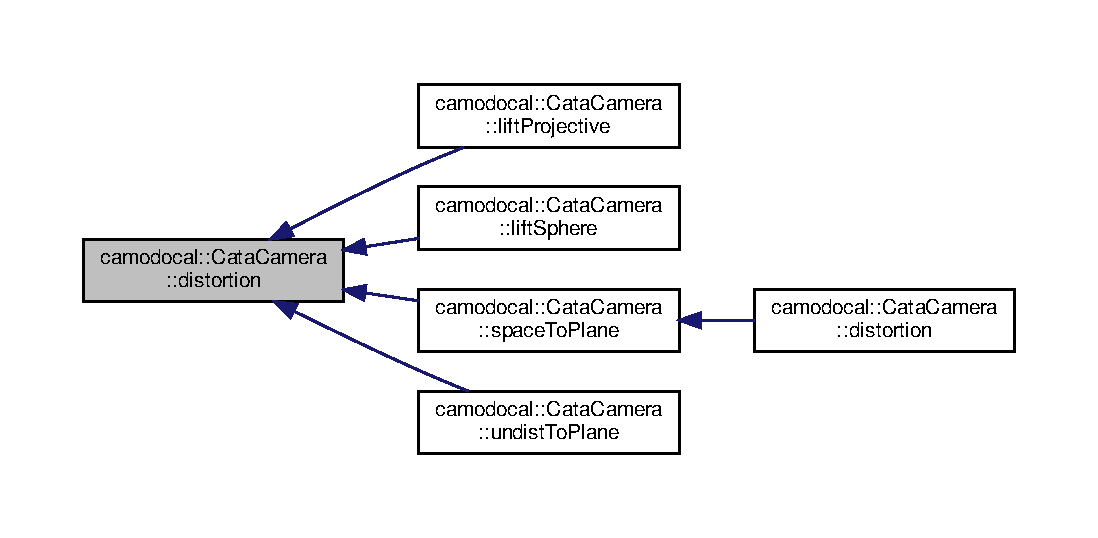
\includegraphics[width=350pt]{classcamodocal_1_1CataCamera_ade73e1a665f97d5a95d09f0fff19a3f7_icgraph}
\end{center}
\end{figure}
\mbox{\Hypertarget{classcamodocal_1_1CataCamera_af9f94a9e9109ad71fcabb0f7bc77a18f}\label{classcamodocal_1_1CataCamera_af9f94a9e9109ad71fcabb0f7bc77a18f}} 
\index{camodocal\+::\+Cata\+Camera@{camodocal\+::\+Cata\+Camera}!distortion@{distortion}}
\index{distortion@{distortion}!camodocal\+::\+Cata\+Camera@{camodocal\+::\+Cata\+Camera}}
\subsubsection{\texorpdfstring{distortion()}{distortion()}\hspace{0.1cm}{\footnotesize\ttfamily [2/2]}}
{\footnotesize\ttfamily void camodocal\+::\+Cata\+Camera\+::distortion (\begin{DoxyParamCaption}\item[{const Eigen\+::\+Vector2d \&}]{p\+\_\+u,  }\item[{Eigen\+::\+Vector2d \&}]{d\+\_\+u,  }\item[{Eigen\+::\+Matrix2d \&}]{J }\end{DoxyParamCaption}) const}



Apply distortion to input point (from the normalised plane) and calculate Jacobian. 


\begin{DoxyParams}{Parameters}
{\em p\+\_\+u} & undistorted coordinates of point on the normalised plane \\
\hline
\end{DoxyParams}
\begin{DoxyReturn}{Returns}
to obtain the distorted point\+: p\+\_\+d = p\+\_\+u + d\+\_\+u 
\end{DoxyReturn}


References camodocal\+::\+Camera\+::\+Parameters\+::image\+Height(), camodocal\+::\+Camera\+::\+Parameters\+::image\+Width(), and space\+To\+Plane().

Here is the call graph for this function\+:\nopagebreak
\begin{figure}[H]
\begin{center}
\leavevmode
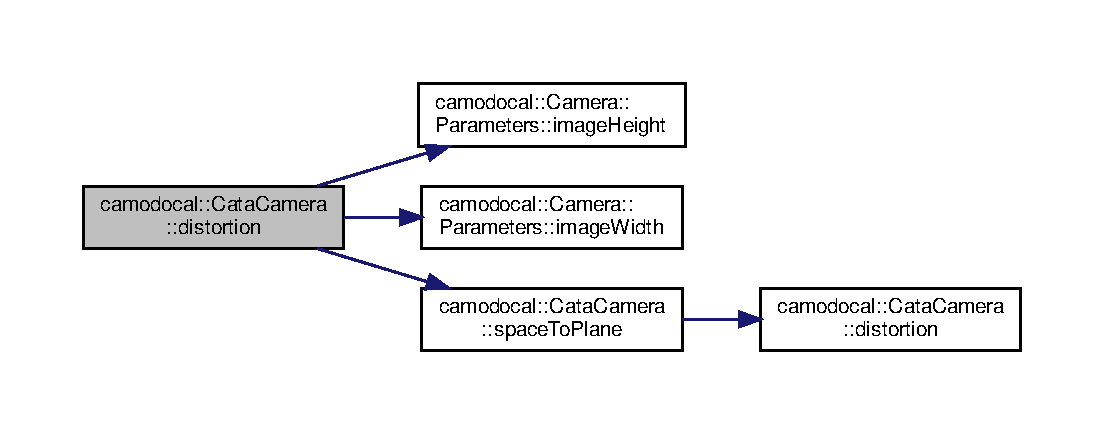
\includegraphics[width=350pt]{classcamodocal_1_1CataCamera_af9f94a9e9109ad71fcabb0f7bc77a18f_cgraph}
\end{center}
\end{figure}
\mbox{\Hypertarget{classcamodocal_1_1CataCamera_a8415dca7d06b730a0b7358745aaa4001}\label{classcamodocal_1_1CataCamera_a8415dca7d06b730a0b7358745aaa4001}} 
\index{camodocal\+::\+Cata\+Camera@{camodocal\+::\+Cata\+Camera}!lift\+Projective@{lift\+Projective}}
\index{lift\+Projective@{lift\+Projective}!camodocal\+::\+Cata\+Camera@{camodocal\+::\+Cata\+Camera}}
\subsubsection{\texorpdfstring{lift\+Projective()}{liftProjective()}}
{\footnotesize\ttfamily void camodocal\+::\+Cata\+Camera\+::lift\+Projective (\begin{DoxyParamCaption}\item[{const Eigen\+::\+Vector2d \&}]{p,  }\item[{Eigen\+::\+Vector3d \&}]{P }\end{DoxyParamCaption}) const\hspace{0.3cm}{\ttfamily [virtual]}}



Lifts a point from the image plane to its projective ray. 


\begin{DoxyParams}{Parameters}
{\em p} & image coordinates \\
\hline
{\em P} & coordinates of the projective ray \\
\hline
\end{DoxyParams}


Implements \hyperlink{classcamodocal_1_1Camera_a680e97bfecab33cd833f914ee811d12d}{camodocal\+::\+Camera}.



References distortion().

Here is the call graph for this function\+:\nopagebreak
\begin{figure}[H]
\begin{center}
\leavevmode
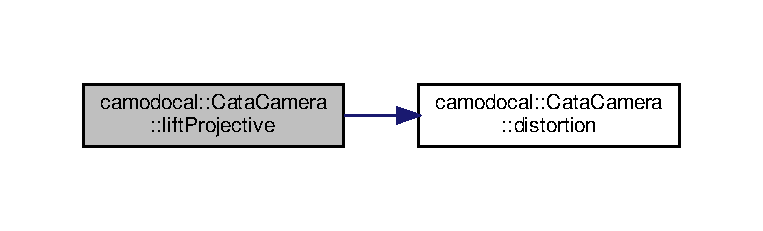
\includegraphics[width=350pt]{classcamodocal_1_1CataCamera_a8415dca7d06b730a0b7358745aaa4001_cgraph}
\end{center}
\end{figure}
\mbox{\Hypertarget{classcamodocal_1_1CataCamera_ad408a25dbeabac661788d16357b44504}\label{classcamodocal_1_1CataCamera_ad408a25dbeabac661788d16357b44504}} 
\index{camodocal\+::\+Cata\+Camera@{camodocal\+::\+Cata\+Camera}!lift\+Sphere@{lift\+Sphere}}
\index{lift\+Sphere@{lift\+Sphere}!camodocal\+::\+Cata\+Camera@{camodocal\+::\+Cata\+Camera}}
\subsubsection{\texorpdfstring{lift\+Sphere()}{liftSphere()}}
{\footnotesize\ttfamily void camodocal\+::\+Cata\+Camera\+::lift\+Sphere (\begin{DoxyParamCaption}\item[{const Eigen\+::\+Vector2d \&}]{p,  }\item[{Eigen\+::\+Vector3d \&}]{P }\end{DoxyParamCaption}) const\hspace{0.3cm}{\ttfamily [virtual]}}



Lifts a point from the image plane to the unit sphere. 


\begin{DoxyParams}{Parameters}
{\em p} & image coordinates \\
\hline
{\em P} & coordinates of the point on the sphere \\
\hline
\end{DoxyParams}


Implements \hyperlink{classcamodocal_1_1Camera_a77b4ea673c694741302efba6f86a0100}{camodocal\+::\+Camera}.



References distortion().

Here is the call graph for this function\+:\nopagebreak
\begin{figure}[H]
\begin{center}
\leavevmode
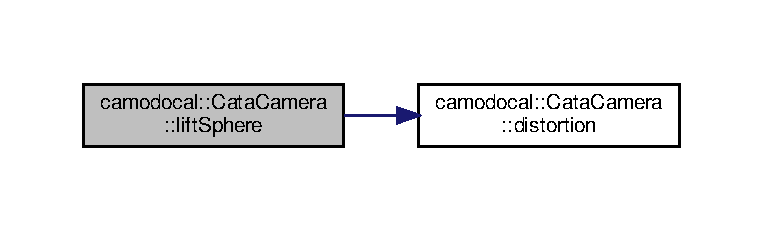
\includegraphics[width=350pt]{classcamodocal_1_1CataCamera_ad408a25dbeabac661788d16357b44504_cgraph}
\end{center}
\end{figure}
\mbox{\Hypertarget{classcamodocal_1_1CataCamera_ab705d867d93d87c85d755bb7b1022a2c}\label{classcamodocal_1_1CataCamera_ab705d867d93d87c85d755bb7b1022a2c}} 
\index{camodocal\+::\+Cata\+Camera@{camodocal\+::\+Cata\+Camera}!space\+To\+Plane@{space\+To\+Plane}}
\index{space\+To\+Plane@{space\+To\+Plane}!camodocal\+::\+Cata\+Camera@{camodocal\+::\+Cata\+Camera}}
\subsubsection{\texorpdfstring{space\+To\+Plane()}{spaceToPlane()}}
{\footnotesize\ttfamily void camodocal\+::\+Cata\+Camera\+::space\+To\+Plane (\begin{DoxyParamCaption}\item[{const Eigen\+::\+Vector3d \&}]{P,  }\item[{Eigen\+::\+Vector2d \&}]{p }\end{DoxyParamCaption}) const\hspace{0.3cm}{\ttfamily [virtual]}}



Project a 3D point ({\itshape x},{\itshape y},{\itshape z}) to the image plane in ({\itshape u},{\itshape v}) 


\begin{DoxyParams}{Parameters}
{\em P} & 3D point coordinates \\
\hline
{\em p} & return value, contains the image point coordinates \\
\hline
\end{DoxyParams}


Implements \hyperlink{classcamodocal_1_1Camera_acf49bd1ef0919e0faf89d060dc497b52}{camodocal\+::\+Camera}.



References distortion().



Referenced by distortion().

Here is the call graph for this function\+:\nopagebreak
\begin{figure}[H]
\begin{center}
\leavevmode
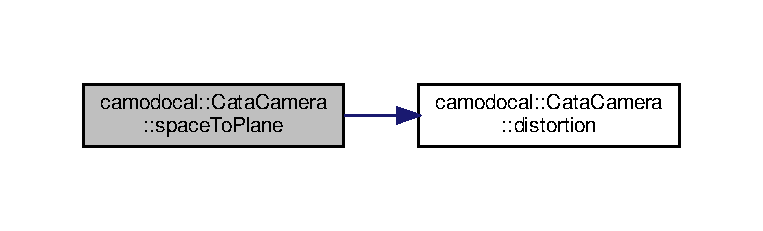
\includegraphics[width=350pt]{classcamodocal_1_1CataCamera_ab705d867d93d87c85d755bb7b1022a2c_cgraph}
\end{center}
\end{figure}
Here is the caller graph for this function\+:\nopagebreak
\begin{figure}[H]
\begin{center}
\leavevmode
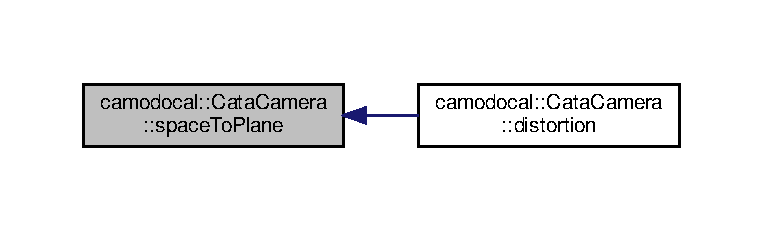
\includegraphics[width=350pt]{classcamodocal_1_1CataCamera_ab705d867d93d87c85d755bb7b1022a2c_icgraph}
\end{center}
\end{figure}
\mbox{\Hypertarget{classcamodocal_1_1CataCamera_a9184557401622acaf2a00fd9b1295d13}\label{classcamodocal_1_1CataCamera_a9184557401622acaf2a00fd9b1295d13}} 
\index{camodocal\+::\+Cata\+Camera@{camodocal\+::\+Cata\+Camera}!undist\+To\+Plane@{undist\+To\+Plane}}
\index{undist\+To\+Plane@{undist\+To\+Plane}!camodocal\+::\+Cata\+Camera@{camodocal\+::\+Cata\+Camera}}
\subsubsection{\texorpdfstring{undist\+To\+Plane()}{undistToPlane()}}
{\footnotesize\ttfamily void camodocal\+::\+Cata\+Camera\+::undist\+To\+Plane (\begin{DoxyParamCaption}\item[{const Eigen\+::\+Vector2d \&}]{p\+\_\+u,  }\item[{Eigen\+::\+Vector2d \&}]{p }\end{DoxyParamCaption}) const\hspace{0.3cm}{\ttfamily [virtual]}}



Projects an undistorted 2D point p\+\_\+u to the image plane. 


\begin{DoxyParams}{Parameters}
{\em p\+\_\+u} & 2D point coordinates \\
\hline
\end{DoxyParams}
\begin{DoxyReturn}{Returns}
image point coordinates 
\end{DoxyReturn}


Implements \hyperlink{classcamodocal_1_1Camera}{camodocal\+::\+Camera}.



References distortion().

Here is the call graph for this function\+:\nopagebreak
\begin{figure}[H]
\begin{center}
\leavevmode
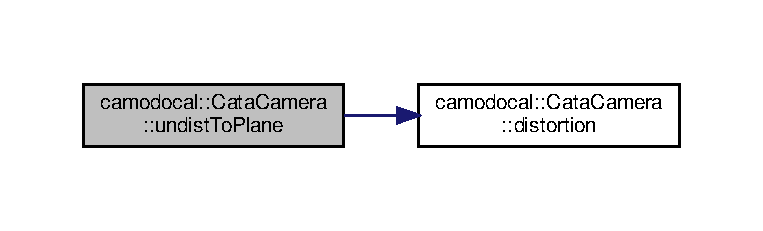
\includegraphics[width=350pt]{classcamodocal_1_1CataCamera_a9184557401622acaf2a00fd9b1295d13_cgraph}
\end{center}
\end{figure}


The documentation for this class was generated from the following files\+:\begin{DoxyCompactItemize}
\item 
camera\+\_\+model/include/camodocal/camera\+\_\+models/Cata\+Camera.\+h\item 
camera\+\_\+model/src/camera\+\_\+models/Cata\+Camera.\+cc\end{DoxyCompactItemize}

\hypertarget{classcamodocal_1_1Chessboard}{}\section{camodocal\+:\+:Chessboard Class Reference}
\label{classcamodocal_1_1Chessboard}\index{camodocal\+::\+Chessboard@{camodocal\+::\+Chessboard}}
\subsection*{Public Member Functions}
\begin{DoxyCompactItemize}
\item 
\mbox{\Hypertarget{classcamodocal_1_1Chessboard_ad78c50ec12b5add1690415d36085d7f3}\label{classcamodocal_1_1Chessboard_ad78c50ec12b5add1690415d36085d7f3}} 
{\bfseries Chessboard} (cv\+::\+Size board\+Size, cv\+::\+Mat \&image)
\item 
\mbox{\Hypertarget{classcamodocal_1_1Chessboard_afaf550f0cd4114c43fbd8d06fa5fcbba}\label{classcamodocal_1_1Chessboard_afaf550f0cd4114c43fbd8d06fa5fcbba}} 
void {\bfseries find\+Corners} (bool use\+Open\+CV=false)
\item 
\mbox{\Hypertarget{classcamodocal_1_1Chessboard_a67d30c45147a8b5425a7295aafac4e67}\label{classcamodocal_1_1Chessboard_a67d30c45147a8b5425a7295aafac4e67}} 
const std\+::vector$<$ cv\+::\+Point2f $>$ \& {\bfseries get\+Corners} (void) const
\item 
\mbox{\Hypertarget{classcamodocal_1_1Chessboard_a849f42f290405858b43b84317769a9e2}\label{classcamodocal_1_1Chessboard_a849f42f290405858b43b84317769a9e2}} 
bool {\bfseries corners\+Found} (void) const
\item 
\mbox{\Hypertarget{classcamodocal_1_1Chessboard_a07f0d320f0855d03167e992fa49eb6ec}\label{classcamodocal_1_1Chessboard_a07f0d320f0855d03167e992fa49eb6ec}} 
const cv\+::\+Mat \& {\bfseries get\+Image} (void) const
\item 
\mbox{\Hypertarget{classcamodocal_1_1Chessboard_a182cc0e7fb1b96336d92cbc6bf626b98}\label{classcamodocal_1_1Chessboard_a182cc0e7fb1b96336d92cbc6bf626b98}} 
const cv\+::\+Mat \& {\bfseries get\+Sketch} (void) const
\end{DoxyCompactItemize}


The documentation for this class was generated from the following files\+:\begin{DoxyCompactItemize}
\item 
camera\+\_\+model/include/camodocal/chessboard/Chessboard.\+h\item 
camera\+\_\+model/src/chessboard/Chessboard.\+cc\end{DoxyCompactItemize}

\hypertarget{classcamodocal_1_1ChessboardCorner}{}\section{camodocal\+:\+:Chessboard\+Corner Class Reference}
\label{classcamodocal_1_1ChessboardCorner}\index{camodocal\+::\+Chessboard\+Corner@{camodocal\+::\+Chessboard\+Corner}}
\subsection*{Public Member Functions}
\begin{DoxyCompactItemize}
\item 
\mbox{\Hypertarget{classcamodocal_1_1ChessboardCorner_ad0f97fd79d023038737d6922d79a0dc1}\label{classcamodocal_1_1ChessboardCorner_ad0f97fd79d023038737d6922d79a0dc1}} 
float {\bfseries mean\+Dist} (int \&n) const
\end{DoxyCompactItemize}
\subsection*{Public Attributes}
\begin{DoxyCompactItemize}
\item 
\mbox{\Hypertarget{classcamodocal_1_1ChessboardCorner_ace70f702045e28b91d579000d33d9cc6}\label{classcamodocal_1_1ChessboardCorner_ace70f702045e28b91d579000d33d9cc6}} 
cv\+::\+Point2f {\bfseries pt}
\item 
\mbox{\Hypertarget{classcamodocal_1_1ChessboardCorner_ae07b0b6c9259e801201bf1c335c62e26}\label{classcamodocal_1_1ChessboardCorner_ae07b0b6c9259e801201bf1c335c62e26}} 
int {\bfseries row}
\item 
\mbox{\Hypertarget{classcamodocal_1_1ChessboardCorner_af0e21c0c1d5c63a7e53a0d77028a907d}\label{classcamodocal_1_1ChessboardCorner_af0e21c0c1d5c63a7e53a0d77028a907d}} 
int {\bfseries column}
\item 
\mbox{\Hypertarget{classcamodocal_1_1ChessboardCorner_a37896d01a5e3dac13ec68acc83b55d8e}\label{classcamodocal_1_1ChessboardCorner_a37896d01a5e3dac13ec68acc83b55d8e}} 
bool {\bfseries needs\+Neighbor}
\item 
\mbox{\Hypertarget{classcamodocal_1_1ChessboardCorner_a45b6cb99f887343dc5db9e7844460c78}\label{classcamodocal_1_1ChessboardCorner_a45b6cb99f887343dc5db9e7844460c78}} 
int {\bfseries count}
\item 
\mbox{\Hypertarget{classcamodocal_1_1ChessboardCorner_ab8f8803979b0198d0ea222110a75dee8}\label{classcamodocal_1_1ChessboardCorner_ab8f8803979b0198d0ea222110a75dee8}} 
Chessboard\+Corner\+Ptr {\bfseries neighbors} \mbox{[}4\mbox{]}
\end{DoxyCompactItemize}


The documentation for this class was generated from the following file\+:\begin{DoxyCompactItemize}
\item 
camera\+\_\+model/include/camodocal/chessboard/Chessboard\+Corner.\+h\end{DoxyCompactItemize}

\hypertarget{classcamodocal_1_1ChessboardQuad}{}\section{camodocal\+:\+:Chessboard\+Quad Class Reference}
\label{classcamodocal_1_1ChessboardQuad}\index{camodocal\+::\+Chessboard\+Quad@{camodocal\+::\+Chessboard\+Quad}}
\subsection*{Public Attributes}
\begin{DoxyCompactItemize}
\item 
\mbox{\Hypertarget{classcamodocal_1_1ChessboardQuad_aed35e8dd71b415587a19cbb6c983c32b}\label{classcamodocal_1_1ChessboardQuad_aed35e8dd71b415587a19cbb6c983c32b}} 
int {\bfseries count}
\item 
\mbox{\Hypertarget{classcamodocal_1_1ChessboardQuad_a2fd593afa16914e6a7c083c884707174}\label{classcamodocal_1_1ChessboardQuad_a2fd593afa16914e6a7c083c884707174}} 
int {\bfseries group\+\_\+idx}
\item 
\mbox{\Hypertarget{classcamodocal_1_1ChessboardQuad_a7fd10c9c5db21c8d3f687dd487d1c87b}\label{classcamodocal_1_1ChessboardQuad_a7fd10c9c5db21c8d3f687dd487d1c87b}} 
float {\bfseries edge\+\_\+len}
\item 
\mbox{\Hypertarget{classcamodocal_1_1ChessboardQuad_a01a4a0853a20b632cd699753408b07e5}\label{classcamodocal_1_1ChessboardQuad_a01a4a0853a20b632cd699753408b07e5}} 
Chessboard\+Corner\+Ptr {\bfseries corners} \mbox{[}4\mbox{]}
\item 
\mbox{\Hypertarget{classcamodocal_1_1ChessboardQuad_af51a4f6d2b1a587a1073cc300588ac92}\label{classcamodocal_1_1ChessboardQuad_af51a4f6d2b1a587a1073cc300588ac92}} 
Chessboard\+Quad\+Ptr {\bfseries neighbors} \mbox{[}4\mbox{]}
\item 
\mbox{\Hypertarget{classcamodocal_1_1ChessboardQuad_a7412b07c4da71f8c80f5267a1c7ae342}\label{classcamodocal_1_1ChessboardQuad_a7412b07c4da71f8c80f5267a1c7ae342}} 
bool {\bfseries labeled}
\end{DoxyCompactItemize}


The documentation for this class was generated from the following file\+:\begin{DoxyCompactItemize}
\item 
camera\+\_\+model/include/camodocal/chessboard/Chessboard\+Quad.\+h\end{DoxyCompactItemize}

\hypertarget{classcamodocal_1_1ComprehensionError}{}\section{camodocal\+:\+:Comprehension\+Error$<$ CameraT $>$ Class Template Reference}
\label{classcamodocal_1_1ComprehensionError}\index{camodocal\+::\+Comprehension\+Error$<$ Camera\+T $>$@{camodocal\+::\+Comprehension\+Error$<$ Camera\+T $>$}}
\subsection*{Public Member Functions}
\begin{DoxyCompactItemize}
\item 
\mbox{\Hypertarget{classcamodocal_1_1ComprehensionError_ac752cd669997ffc76e1d2c2163804182}\label{classcamodocal_1_1ComprehensionError_ac752cd669997ffc76e1d2c2163804182}} 
E\+I\+G\+E\+N\+\_\+\+M\+A\+K\+E\+\_\+\+A\+L\+I\+G\+N\+E\+D\+\_\+\+O\+P\+E\+R\+A\+T\+O\+R\+\_\+\+N\+EW {\bfseries Comprehension\+Error} (const Eigen\+::\+Vector3d \&observed\+\_\+P, const Eigen\+::\+Vector2d \&observed\+\_\+p)
\item 
\mbox{\Hypertarget{classcamodocal_1_1ComprehensionError_ad9a8971ba9336b8b38178b07b69822b6}\label{classcamodocal_1_1ComprehensionError_ad9a8971ba9336b8b38178b07b69822b6}} 
{\footnotesize template$<$typename T $>$ }\\bool {\bfseries operator()} (const T $\ast$const intrinsic\+\_\+params, const T $\ast$const q, const T $\ast$const t, T $\ast$residuals) const
\end{DoxyCompactItemize}
\subsection*{Public Attributes}
\begin{DoxyCompactItemize}
\item 
\mbox{\Hypertarget{classcamodocal_1_1ComprehensionError_a5614ebe2c0f896e1ed4f82604d2112ee}\label{classcamodocal_1_1ComprehensionError_a5614ebe2c0f896e1ed4f82604d2112ee}} 
Eigen\+::\+Vector3d {\bfseries m\+\_\+observed\+\_\+P}
\item 
\mbox{\Hypertarget{classcamodocal_1_1ComprehensionError_a498f32b3b4466b94339a0cb361b6f1f0}\label{classcamodocal_1_1ComprehensionError_a498f32b3b4466b94339a0cb361b6f1f0}} 
Eigen\+::\+Vector2d {\bfseries m\+\_\+observed\+\_\+p}
\item 
\mbox{\Hypertarget{classcamodocal_1_1ComprehensionError_a2e6556951a4f4967089f090f248cd236}\label{classcamodocal_1_1ComprehensionError_a2e6556951a4f4967089f090f248cd236}} 
Eigen\+::\+Matrix2d {\bfseries m\+\_\+sqrt\+Precision\+Mat}
\end{DoxyCompactItemize}


The documentation for this class was generated from the following file\+:\begin{DoxyCompactItemize}
\item 
camera\+\_\+model/src/camera\+\_\+models/Cost\+Function\+Factory.\+cc\end{DoxyCompactItemize}

\hypertarget{classcamodocal_1_1CostFunctionFactory}{}\section{camodocal\+:\+:Cost\+Function\+Factory Class Reference}
\label{classcamodocal_1_1CostFunctionFactory}\index{camodocal\+::\+Cost\+Function\+Factory@{camodocal\+::\+Cost\+Function\+Factory}}
\subsection*{Public Member Functions}
\begin{DoxyCompactItemize}
\item 
\mbox{\Hypertarget{classcamodocal_1_1CostFunctionFactory_adda465ef8c4f2fa757fd0675f9429d36}\label{classcamodocal_1_1CostFunctionFactory_adda465ef8c4f2fa757fd0675f9429d36}} 
ceres\+::\+Cost\+Function $\ast$ {\bfseries generate\+Cost\+Function} (const \hyperlink{Camera_8h_a03fe5d6885a007cb4ad26d11f6198586}{Camera\+Const\+Ptr} \&camera, const Eigen\+::\+Vector3d \&observed\+\_\+P, const Eigen\+::\+Vector2d \&observed\+\_\+p, int flags) const
\item 
\mbox{\Hypertarget{classcamodocal_1_1CostFunctionFactory_abcea9742c67b6d31d373a538ec167e2c}\label{classcamodocal_1_1CostFunctionFactory_abcea9742c67b6d31d373a538ec167e2c}} 
ceres\+::\+Cost\+Function $\ast$ {\bfseries generate\+Cost\+Function} (const \hyperlink{Camera_8h_a03fe5d6885a007cb4ad26d11f6198586}{Camera\+Const\+Ptr} \&camera, const Eigen\+::\+Vector3d \&observed\+\_\+P, const Eigen\+::\+Vector2d \&observed\+\_\+p, const Eigen\+::\+Matrix2d \&sqrt\+Precision\+Mat, int flags) const
\item 
\mbox{\Hypertarget{classcamodocal_1_1CostFunctionFactory_a8c8da1112f113d2d0ac6e08b23d5303f}\label{classcamodocal_1_1CostFunctionFactory_a8c8da1112f113d2d0ac6e08b23d5303f}} 
ceres\+::\+Cost\+Function $\ast$ {\bfseries generate\+Cost\+Function} (const \hyperlink{Camera_8h_a03fe5d6885a007cb4ad26d11f6198586}{Camera\+Const\+Ptr} \&camera, const Eigen\+::\+Vector2d \&observed\+\_\+p, int flags, bool optimize\+\_\+cam\+\_\+odo\+\_\+z=true) const
\item 
\mbox{\Hypertarget{classcamodocal_1_1CostFunctionFactory_a2c7a3edbb6f2aba03451c687002ea5c5}\label{classcamodocal_1_1CostFunctionFactory_a2c7a3edbb6f2aba03451c687002ea5c5}} 
ceres\+::\+Cost\+Function $\ast$ {\bfseries generate\+Cost\+Function} (const \hyperlink{Camera_8h_a03fe5d6885a007cb4ad26d11f6198586}{Camera\+Const\+Ptr} \&camera, const Eigen\+::\+Vector2d \&observed\+\_\+p, const Eigen\+::\+Matrix2d \&sqrt\+Precision\+Mat, int flags, bool optimize\+\_\+cam\+\_\+odo\+\_\+z=true) const
\item 
\mbox{\Hypertarget{classcamodocal_1_1CostFunctionFactory_a6fb6f746cc6dfafe614a334c8858e0a8}\label{classcamodocal_1_1CostFunctionFactory_a6fb6f746cc6dfafe614a334c8858e0a8}} 
ceres\+::\+Cost\+Function $\ast$ {\bfseries generate\+Cost\+Function} (const \hyperlink{Camera_8h_a03fe5d6885a007cb4ad26d11f6198586}{Camera\+Const\+Ptr} \&camera, const Eigen\+::\+Vector3d \&odo\+\_\+pos, const Eigen\+::\+Vector3d \&odo\+\_\+att, const Eigen\+::\+Vector2d \&observed\+\_\+p, int flags, bool optimize\+\_\+cam\+\_\+odo\+\_\+z=true) const
\item 
\mbox{\Hypertarget{classcamodocal_1_1CostFunctionFactory_adbbd63cb458cf51847df25591d898705}\label{classcamodocal_1_1CostFunctionFactory_adbbd63cb458cf51847df25591d898705}} 
ceres\+::\+Cost\+Function $\ast$ {\bfseries generate\+Cost\+Function} (const \hyperlink{Camera_8h_a03fe5d6885a007cb4ad26d11f6198586}{Camera\+Const\+Ptr} \&camera, const Eigen\+::\+Quaterniond \&cam\+\_\+odo\+\_\+q, const Eigen\+::\+Vector3d \&cam\+\_\+odo\+\_\+t, const Eigen\+::\+Vector3d \&odo\+\_\+pos, const Eigen\+::\+Vector3d \&odo\+\_\+att, const Eigen\+::\+Vector2d \&observed\+\_\+p, int flags) const
\item 
\mbox{\Hypertarget{classcamodocal_1_1CostFunctionFactory_ad9db356b5c933326629dc9b3383d75da}\label{classcamodocal_1_1CostFunctionFactory_ad9db356b5c933326629dc9b3383d75da}} 
ceres\+::\+Cost\+Function $\ast$ {\bfseries generate\+Cost\+Function} (const \hyperlink{Camera_8h_a03fe5d6885a007cb4ad26d11f6198586}{Camera\+Const\+Ptr} \&camera\+Left, const \hyperlink{Camera_8h_a03fe5d6885a007cb4ad26d11f6198586}{Camera\+Const\+Ptr} \&camera\+Right, const Eigen\+::\+Vector3d \&observed\+\_\+P, const Eigen\+::\+Vector2d \&observed\+\_\+p\+\_\+left, const Eigen\+::\+Vector2d \&observed\+\_\+p\+\_\+right) const
\end{DoxyCompactItemize}
\subsection*{Static Public Member Functions}
\begin{DoxyCompactItemize}
\item 
\mbox{\Hypertarget{classcamodocal_1_1CostFunctionFactory_aad2a8835aa630202ffe2ca9f796385f6}\label{classcamodocal_1_1CostFunctionFactory_aad2a8835aa630202ffe2ca9f796385f6}} 
static boost\+::shared\+\_\+ptr$<$ \hyperlink{classcamodocal_1_1CostFunctionFactory}{Cost\+Function\+Factory} $>$ {\bfseries instance} (void)
\end{DoxyCompactItemize}


The documentation for this class was generated from the following files\+:\begin{DoxyCompactItemize}
\item 
camera\+\_\+model/include/camodocal/camera\+\_\+models/Cost\+Function\+Factory.\+h\item 
camera\+\_\+model/src/camera\+\_\+models/Cost\+Function\+Factory.\+cc\end{DoxyCompactItemize}

\hypertarget{structData}{}\section{Data Struct Reference}
\label{structData}\index{Data@{Data}}
\subsection*{Public Member Functions}
\begin{DoxyCompactItemize}
\item 
\mbox{\Hypertarget{structData_a438cc083234ab745bdb241364f505459}\label{structData_a438cc083234ab745bdb241364f505459}} 
{\bfseries Data} (F\+I\+LE $\ast$f)
\end{DoxyCompactItemize}
\subsection*{Public Attributes}
\begin{DoxyCompactItemize}
\item 
\mbox{\Hypertarget{structData_af30e87c8f576878effbb050b6908352d}\label{structData_af30e87c8f576878effbb050b6908352d}} 
double {\bfseries t}
\item 
\mbox{\Hypertarget{structData_abdcc703465065928081830d1adb8933e}\label{structData_abdcc703465065928081830d1adb8933e}} 
float {\bfseries px}
\item 
\mbox{\Hypertarget{structData_a2e71f3a5743235464467b6ee77c11e3d}\label{structData_a2e71f3a5743235464467b6ee77c11e3d}} 
float {\bfseries py}
\item 
\mbox{\Hypertarget{structData_a7f1461aaa1564d119ecbaebee0bbb039}\label{structData_a7f1461aaa1564d119ecbaebee0bbb039}} 
float {\bfseries pz}
\item 
\mbox{\Hypertarget{structData_a216cf86fa1128b46c577af3b1d5bec7c}\label{structData_a216cf86fa1128b46c577af3b1d5bec7c}} 
float {\bfseries qw}
\item 
\mbox{\Hypertarget{structData_a4e85d2c733cb563db0d33a049b5839a2}\label{structData_a4e85d2c733cb563db0d33a049b5839a2}} 
float {\bfseries qx}
\item 
\mbox{\Hypertarget{structData_afbc9d6f248917946d36cdcc66afbfca9}\label{structData_afbc9d6f248917946d36cdcc66afbfca9}} 
float {\bfseries qy}
\item 
\mbox{\Hypertarget{structData_ad8fad9789bc5dbb5370100318b49ab05}\label{structData_ad8fad9789bc5dbb5370100318b49ab05}} 
float {\bfseries qz}
\item 
\mbox{\Hypertarget{structData_a382ef56cf80be090172065082bda493f}\label{structData_a382ef56cf80be090172065082bda493f}} 
float {\bfseries vx}
\item 
\mbox{\Hypertarget{structData_a0ee23c5cd0d5ed16ba3a6ac75e776eb0}\label{structData_a0ee23c5cd0d5ed16ba3a6ac75e776eb0}} 
float {\bfseries vy}
\item 
\mbox{\Hypertarget{structData_af2969d9014a82586023dccd12c6f869a}\label{structData_af2969d9014a82586023dccd12c6f869a}} 
float {\bfseries vz}
\item 
\mbox{\Hypertarget{structData_a5079f3ccb391d6578615839629dfb58e}\label{structData_a5079f3ccb391d6578615839629dfb58e}} 
float {\bfseries wx}
\item 
\mbox{\Hypertarget{structData_a3c8cbb0ef35204ef048714665127664f}\label{structData_a3c8cbb0ef35204ef048714665127664f}} 
float {\bfseries wy}
\item 
\mbox{\Hypertarget{structData_ab06a01c5e0db3f770d38dddbc2b6172b}\label{structData_ab06a01c5e0db3f770d38dddbc2b6172b}} 
float {\bfseries wz}
\item 
\mbox{\Hypertarget{structData_aedcab7fcf8b055783b9ac3f8d5e00a5e}\label{structData_aedcab7fcf8b055783b9ac3f8d5e00a5e}} 
float {\bfseries ax}
\item 
\mbox{\Hypertarget{structData_af24ed7b872419bd5bca14a7dfcd50561}\label{structData_af24ed7b872419bd5bca14a7dfcd50561}} 
float {\bfseries ay}
\item 
\mbox{\Hypertarget{structData_a88eb7b0726318996110f187a4c94d287}\label{structData_a88eb7b0726318996110f187a4c94d287}} 
float {\bfseries az}
\end{DoxyCompactItemize}


The documentation for this struct was generated from the following file\+:\begin{DoxyCompactItemize}
\item 
benchmark\+\_\+publisher/src/benchmark\+\_\+publisher\+\_\+node.\+cpp\end{DoxyCompactItemize}

\hypertarget{classDUtils_1_1DException}{}\section{D\+Utils\+:\+:D\+Exception Class Reference}
\label{classDUtils_1_1DException}\index{D\+Utils\+::\+D\+Exception@{D\+Utils\+::\+D\+Exception}}


General exception.  




{\ttfamily \#include $<$D\+Exception.\+h$>$}



Inheritance diagram for D\+Utils\+:\+:D\+Exception\+:\nopagebreak
\begin{figure}[H]
\begin{center}
\leavevmode
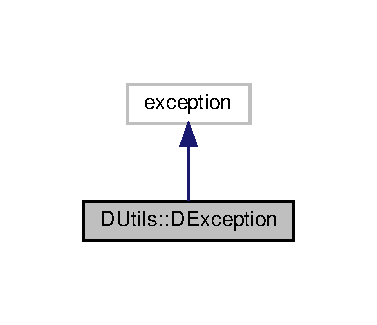
\includegraphics[width=181pt]{classDUtils_1_1DException__inherit__graph}
\end{center}
\end{figure}


Collaboration diagram for D\+Utils\+:\+:D\+Exception\+:\nopagebreak
\begin{figure}[H]
\begin{center}
\leavevmode
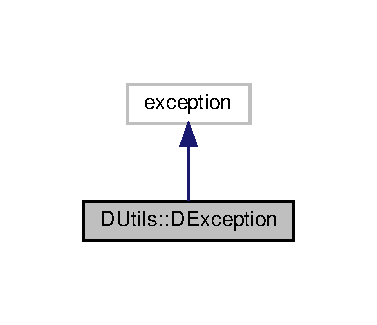
\includegraphics[width=181pt]{classDUtils_1_1DException__coll__graph}
\end{center}
\end{figure}
\subsection*{Public Member Functions}
\begin{DoxyCompactItemize}
\item 
\hyperlink{classDUtils_1_1DException_a2a7b85153de7d01a46606271c32254ce}{D\+Exception} (void)  throw ()
\item 
\hyperlink{classDUtils_1_1DException_aba7bdd9f0c908590dc48cfacb50efc56}{D\+Exception} (const char $\ast$msg)  throw ()
\item 
\hyperlink{classDUtils_1_1DException_a611f325f78d0e79b3bac5234b3f9ff99}{D\+Exception} (const string \&msg)  throw ()
\item 
virtual \hyperlink{classDUtils_1_1DException_a12deb785f50e9cb2db3541ffb60a20bb}{$\sim$\+D\+Exception} (void)  throw ()
\item 
virtual const char $\ast$ \hyperlink{classDUtils_1_1DException_ad5d0ccb4bf61cdb3e23b2b5b9e1a402c}{what} () const  throw ()
\end{DoxyCompactItemize}
\subsection*{Protected Attributes}
\begin{DoxyCompactItemize}
\item 
\mbox{\Hypertarget{classDUtils_1_1DException_ab31e6216df2034af61edb32632006bfb}\label{classDUtils_1_1DException_ab31e6216df2034af61edb32632006bfb}} 
string \hyperlink{classDUtils_1_1DException_ab31e6216df2034af61edb32632006bfb}{m\+\_\+message}
\begin{DoxyCompactList}\small\item\em Error message. \end{DoxyCompactList}\end{DoxyCompactItemize}


\subsection{Detailed Description}
General exception. 

\subsection{Constructor \& Destructor Documentation}
\mbox{\Hypertarget{classDUtils_1_1DException_a2a7b85153de7d01a46606271c32254ce}\label{classDUtils_1_1DException_a2a7b85153de7d01a46606271c32254ce}} 
\index{D\+Utils\+::\+D\+Exception@{D\+Utils\+::\+D\+Exception}!D\+Exception@{D\+Exception}}
\index{D\+Exception@{D\+Exception}!D\+Utils\+::\+D\+Exception@{D\+Utils\+::\+D\+Exception}}
\subsubsection{\texorpdfstring{D\+Exception()}{DException()}\hspace{0.1cm}{\footnotesize\ttfamily [1/3]}}
{\footnotesize\ttfamily D\+Utils\+::\+D\+Exception\+::\+D\+Exception (\begin{DoxyParamCaption}\item[{void}]{ }\end{DoxyParamCaption}) throw  ) \hspace{0.3cm}{\ttfamily [inline]}}

Creates an exception with a general error message \mbox{\Hypertarget{classDUtils_1_1DException_aba7bdd9f0c908590dc48cfacb50efc56}\label{classDUtils_1_1DException_aba7bdd9f0c908590dc48cfacb50efc56}} 
\index{D\+Utils\+::\+D\+Exception@{D\+Utils\+::\+D\+Exception}!D\+Exception@{D\+Exception}}
\index{D\+Exception@{D\+Exception}!D\+Utils\+::\+D\+Exception@{D\+Utils\+::\+D\+Exception}}
\subsubsection{\texorpdfstring{D\+Exception()}{DException()}\hspace{0.1cm}{\footnotesize\ttfamily [2/3]}}
{\footnotesize\ttfamily D\+Utils\+::\+D\+Exception\+::\+D\+Exception (\begin{DoxyParamCaption}\item[{const char $\ast$}]{msg }\end{DoxyParamCaption}) throw  ) \hspace{0.3cm}{\ttfamily [inline]}}

Creates an exception with a custom error message 
\begin{DoxyParams}{Parameters}
{\em msg} & message \\
\hline
\end{DoxyParams}
\mbox{\Hypertarget{classDUtils_1_1DException_a611f325f78d0e79b3bac5234b3f9ff99}\label{classDUtils_1_1DException_a611f325f78d0e79b3bac5234b3f9ff99}} 
\index{D\+Utils\+::\+D\+Exception@{D\+Utils\+::\+D\+Exception}!D\+Exception@{D\+Exception}}
\index{D\+Exception@{D\+Exception}!D\+Utils\+::\+D\+Exception@{D\+Utils\+::\+D\+Exception}}
\subsubsection{\texorpdfstring{D\+Exception()}{DException()}\hspace{0.1cm}{\footnotesize\ttfamily [3/3]}}
{\footnotesize\ttfamily D\+Utils\+::\+D\+Exception\+::\+D\+Exception (\begin{DoxyParamCaption}\item[{const string \&}]{msg }\end{DoxyParamCaption}) throw  ) \hspace{0.3cm}{\ttfamily [inline]}}

Creates an exception with a custom error message 
\begin{DoxyParams}{Parameters}
{\em msg} & message \\
\hline
\end{DoxyParams}
\mbox{\Hypertarget{classDUtils_1_1DException_a12deb785f50e9cb2db3541ffb60a20bb}\label{classDUtils_1_1DException_a12deb785f50e9cb2db3541ffb60a20bb}} 
\index{D\+Utils\+::\+D\+Exception@{D\+Utils\+::\+D\+Exception}!````~D\+Exception@{$\sim$\+D\+Exception}}
\index{````~D\+Exception@{$\sim$\+D\+Exception}!D\+Utils\+::\+D\+Exception@{D\+Utils\+::\+D\+Exception}}
\subsubsection{\texorpdfstring{$\sim$\+D\+Exception()}{~DException()}}
{\footnotesize\ttfamily virtual D\+Utils\+::\+D\+Exception\+::$\sim$\+D\+Exception (\begin{DoxyParamCaption}\item[{void}]{ }\end{DoxyParamCaption}) throw  ) \hspace{0.3cm}{\ttfamily [inline]}, {\ttfamily [virtual]}}

Destructor 

\subsection{Member Function Documentation}
\mbox{\Hypertarget{classDUtils_1_1DException_ad5d0ccb4bf61cdb3e23b2b5b9e1a402c}\label{classDUtils_1_1DException_ad5d0ccb4bf61cdb3e23b2b5b9e1a402c}} 
\index{D\+Utils\+::\+D\+Exception@{D\+Utils\+::\+D\+Exception}!what@{what}}
\index{what@{what}!D\+Utils\+::\+D\+Exception@{D\+Utils\+::\+D\+Exception}}
\subsubsection{\texorpdfstring{what()}{what()}}
{\footnotesize\ttfamily virtual const char$\ast$ D\+Utils\+::\+D\+Exception\+::what (\begin{DoxyParamCaption}{ }\end{DoxyParamCaption}) const throw  ) \hspace{0.3cm}{\ttfamily [inline]}, {\ttfamily [virtual]}}

Returns the exception message 

The documentation for this class was generated from the following file\+:\begin{DoxyCompactItemize}
\item 
pose\+\_\+graph/src/\+Third\+Party/\+D\+Utils/D\+Exception.\+h\end{DoxyCompactItemize}

\hypertarget{classcamodocal_1_1EigenQuaternionParameterization}{}\section{camodocal\+:\+:Eigen\+Quaternion\+Parameterization Class Reference}
\label{classcamodocal_1_1EigenQuaternionParameterization}\index{camodocal\+::\+Eigen\+Quaternion\+Parameterization@{camodocal\+::\+Eigen\+Quaternion\+Parameterization}}


Inheritance diagram for camodocal\+:\+:Eigen\+Quaternion\+Parameterization\+:\nopagebreak
\begin{figure}[H]
\begin{center}
\leavevmode
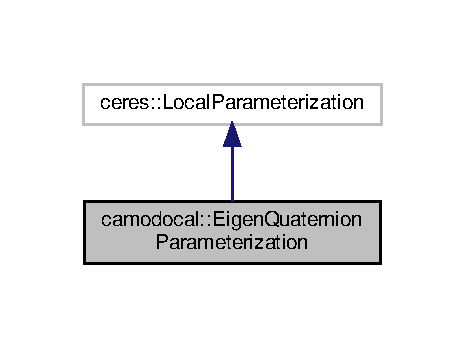
\includegraphics[width=223pt]{classcamodocal_1_1EigenQuaternionParameterization__inherit__graph}
\end{center}
\end{figure}


Collaboration diagram for camodocal\+:\+:Eigen\+Quaternion\+Parameterization\+:\nopagebreak
\begin{figure}[H]
\begin{center}
\leavevmode
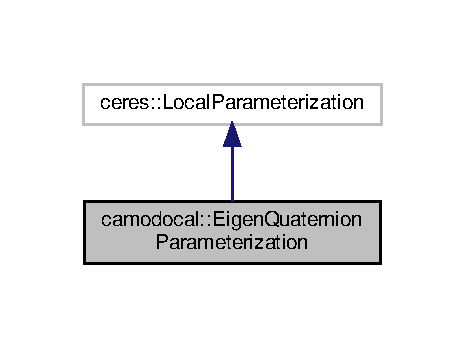
\includegraphics[width=223pt]{classcamodocal_1_1EigenQuaternionParameterization__coll__graph}
\end{center}
\end{figure}
\subsection*{Public Member Functions}
\begin{DoxyCompactItemize}
\item 
\mbox{\Hypertarget{classcamodocal_1_1EigenQuaternionParameterization_a536708d4a3e63f004fc53536bb52a99c}\label{classcamodocal_1_1EigenQuaternionParameterization_a536708d4a3e63f004fc53536bb52a99c}} 
virtual bool {\bfseries Plus} (const double $\ast$x, const double $\ast$delta, double $\ast$x\+\_\+plus\+\_\+delta) const
\item 
\mbox{\Hypertarget{classcamodocal_1_1EigenQuaternionParameterization_a86731e8edac30b9b5dfc3b0c8d49eef4}\label{classcamodocal_1_1EigenQuaternionParameterization_a86731e8edac30b9b5dfc3b0c8d49eef4}} 
virtual bool {\bfseries Compute\+Jacobian} (const double $\ast$x, double $\ast$jacobian) const
\item 
\mbox{\Hypertarget{classcamodocal_1_1EigenQuaternionParameterization_a6457c07b1ff1da939422df0de21d5f16}\label{classcamodocal_1_1EigenQuaternionParameterization_a6457c07b1ff1da939422df0de21d5f16}} 
virtual int {\bfseries Global\+Size} () const
\item 
\mbox{\Hypertarget{classcamodocal_1_1EigenQuaternionParameterization_a7043466bbaca16c7071b73f142ff5581}\label{classcamodocal_1_1EigenQuaternionParameterization_a7043466bbaca16c7071b73f142ff5581}} 
virtual int {\bfseries Local\+Size} () const
\end{DoxyCompactItemize}


The documentation for this class was generated from the following files\+:\begin{DoxyCompactItemize}
\item 
camera\+\_\+model/include/camodocal/gpl/Eigen\+Quaternion\+Parameterization.\+h\item 
camera\+\_\+model/src/gpl/Eigen\+Quaternion\+Parameterization.\+cc\end{DoxyCompactItemize}

\hypertarget{classcamodocal_1_1EquidistantCamera}{}\section{camodocal\+:\+:Equidistant\+Camera Class Reference}
\label{classcamodocal_1_1EquidistantCamera}\index{camodocal\+::\+Equidistant\+Camera@{camodocal\+::\+Equidistant\+Camera}}


{\ttfamily \#include $<$Equidistant\+Camera.\+h$>$}



Inheritance diagram for camodocal\+:\+:Equidistant\+Camera\+:\nopagebreak
\begin{figure}[H]
\begin{center}
\leavevmode
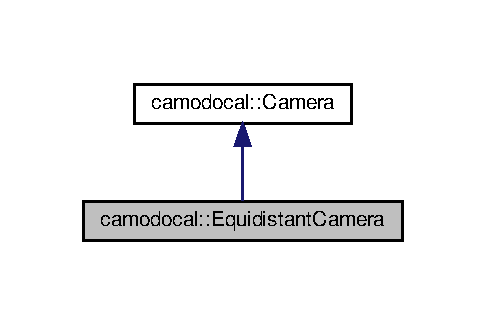
\includegraphics[width=233pt]{classcamodocal_1_1EquidistantCamera__inherit__graph}
\end{center}
\end{figure}


Collaboration diagram for camodocal\+:\+:Equidistant\+Camera\+:\nopagebreak
\begin{figure}[H]
\begin{center}
\leavevmode
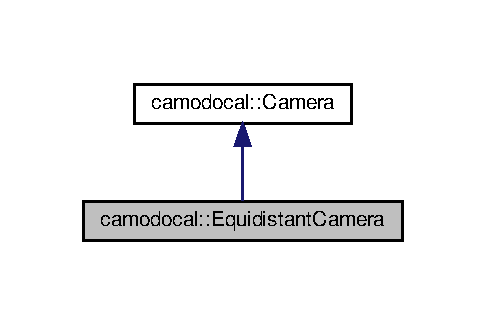
\includegraphics[width=233pt]{classcamodocal_1_1EquidistantCamera__coll__graph}
\end{center}
\end{figure}
\subsection*{Classes}
\begin{DoxyCompactItemize}
\item 
class \hyperlink{classcamodocal_1_1EquidistantCamera_1_1Parameters}{Parameters}
\end{DoxyCompactItemize}
\subsection*{Public Member Functions}
\begin{DoxyCompactItemize}
\item 
\mbox{\Hypertarget{classcamodocal_1_1EquidistantCamera_ad00dbcd6ff79c1a86009fdb168e8f912}\label{classcamodocal_1_1EquidistantCamera_ad00dbcd6ff79c1a86009fdb168e8f912}} 
\hyperlink{classcamodocal_1_1EquidistantCamera_ad00dbcd6ff79c1a86009fdb168e8f912}{Equidistant\+Camera} (const std\+::string \&\hyperlink{classcamodocal_1_1EquidistantCamera_a985ec4cd98fed18f5201551b24cf1d8b}{camera\+Name}, int \hyperlink{classcamodocal_1_1EquidistantCamera_a90ff17672aca7c81cd56d8541cbb3190}{image\+Width}, int \hyperlink{classcamodocal_1_1EquidistantCamera_a7db0d67a1c27897c04e3ae1635207433}{image\+Height}, double k2, double k3, double k4, double k5, double mu, double mv, double u0, double v0)
\begin{DoxyCompactList}\small\item\em Constructor from the projection model parameters. \end{DoxyCompactList}\item 
\mbox{\Hypertarget{classcamodocal_1_1EquidistantCamera_a9f83afd3d68f9cde56e669b62498133f}\label{classcamodocal_1_1EquidistantCamera_a9f83afd3d68f9cde56e669b62498133f}} 
\hyperlink{classcamodocal_1_1EquidistantCamera_a9f83afd3d68f9cde56e669b62498133f}{Equidistant\+Camera} (const \hyperlink{classcamodocal_1_1EquidistantCamera_1_1Parameters}{Parameters} \&params)
\begin{DoxyCompactList}\small\item\em Constructor from the projection model parameters. \end{DoxyCompactList}\item 
\mbox{\Hypertarget{classcamodocal_1_1EquidistantCamera_a5fbae9e11f1bfdc4f8c221b3525c34a6}\label{classcamodocal_1_1EquidistantCamera_a5fbae9e11f1bfdc4f8c221b3525c34a6}} 
\hyperlink{classcamodocal_1_1Camera_a663bb19b7b1f38f6d1b7eeb0890183ff}{Camera\+::\+Model\+Type} \hyperlink{classcamodocal_1_1EquidistantCamera_a5fbae9e11f1bfdc4f8c221b3525c34a6}{model\+Type} (void) const
\begin{DoxyCompactList}\small\item\em virtual type of function model\+Type \end{DoxyCompactList}\item 
\mbox{\Hypertarget{classcamodocal_1_1EquidistantCamera_a985ec4cd98fed18f5201551b24cf1d8b}\label{classcamodocal_1_1EquidistantCamera_a985ec4cd98fed18f5201551b24cf1d8b}} 
const std\+::string \& \hyperlink{classcamodocal_1_1EquidistantCamera_a985ec4cd98fed18f5201551b24cf1d8b}{camera\+Name} (void) const
\begin{DoxyCompactList}\small\item\em virtual type of funtion camera\+Name \end{DoxyCompactList}\item 
\mbox{\Hypertarget{classcamodocal_1_1EquidistantCamera_a90ff17672aca7c81cd56d8541cbb3190}\label{classcamodocal_1_1EquidistantCamera_a90ff17672aca7c81cd56d8541cbb3190}} 
int \hyperlink{classcamodocal_1_1EquidistantCamera_a90ff17672aca7c81cd56d8541cbb3190}{image\+Width} (void) const
\begin{DoxyCompactList}\small\item\em virtual type of function image\+Width \end{DoxyCompactList}\item 
\mbox{\Hypertarget{classcamodocal_1_1EquidistantCamera_a7db0d67a1c27897c04e3ae1635207433}\label{classcamodocal_1_1EquidistantCamera_a7db0d67a1c27897c04e3ae1635207433}} 
int \hyperlink{classcamodocal_1_1EquidistantCamera_a7db0d67a1c27897c04e3ae1635207433}{image\+Height} (void) const
\begin{DoxyCompactList}\small\item\em virtual type of function image\+Height \end{DoxyCompactList}\item 
\mbox{\Hypertarget{classcamodocal_1_1EquidistantCamera_a07be015f3740cb23c1cdd87f3a4ba505}\label{classcamodocal_1_1EquidistantCamera_a07be015f3740cb23c1cdd87f3a4ba505}} 
void \hyperlink{classcamodocal_1_1EquidistantCamera_a07be015f3740cb23c1cdd87f3a4ba505}{estimate\+Intrinsics} (const cv\+::\+Size \&board\+Size, const std\+::vector$<$ std\+::vector$<$ cv\+::\+Point3f $>$ $>$ \&object\+Points, const std\+::vector$<$ std\+::vector$<$ cv\+::\+Point2f $>$ $>$ \&image\+Points)
\begin{DoxyCompactList}\small\item\em virtual function of camera intrinsics \end{DoxyCompactList}\item 
virtual void \hyperlink{classcamodocal_1_1EquidistantCamera_ac86c8527e09b6df4eea4fd3c1322ba00}{lift\+Sphere} (const Eigen\+::\+Vector2d \&p, Eigen\+::\+Vector3d \&P) const
\begin{DoxyCompactList}\small\item\em Lifts a point from the image plane to the unit sphere. \end{DoxyCompactList}\item 
void \hyperlink{classcamodocal_1_1EquidistantCamera_accd38ebf90227cc221d91dad7dd57dbb}{lift\+Projective} (const Eigen\+::\+Vector2d \&p, Eigen\+::\+Vector3d \&P) const
\begin{DoxyCompactList}\small\item\em Lifts a point from the image plane to its projective ray. \end{DoxyCompactList}\item 
void \hyperlink{classcamodocal_1_1EquidistantCamera_a04de4daf1568c2425eabdbade499f927}{space\+To\+Plane} (const Eigen\+::\+Vector3d \&P, Eigen\+::\+Vector2d \&p) const
\begin{DoxyCompactList}\small\item\em Project a 3D point ({\itshape x},{\itshape y},{\itshape z}) to the image plane in ({\itshape u},{\itshape v}) \end{DoxyCompactList}\item 
void \hyperlink{classcamodocal_1_1EquidistantCamera_af24c481afa7e454a687fcdc7726d443f}{space\+To\+Plane} (const Eigen\+::\+Vector3d \&P, Eigen\+::\+Vector2d \&p, Eigen\+::\+Matrix$<$ double, 2, 3 $>$ \&J) const
\begin{DoxyCompactList}\small\item\em Project a 3D point to the image plane and calculate Jacobian. \end{DoxyCompactList}\item 
void \hyperlink{classcamodocal_1_1EquidistantCamera_ac0aae0a472fac59ad5fc22079eb5560d}{undist\+To\+Plane} (const Eigen\+::\+Vector2d \&p\+\_\+u, Eigen\+::\+Vector2d \&p) const
\begin{DoxyCompactList}\small\item\em Projects an undistorted 2D point p\+\_\+u to the image plane. \end{DoxyCompactList}\item 
\mbox{\Hypertarget{classcamodocal_1_1EquidistantCamera_a192665c52e98f0428a5a466565222f39}\label{classcamodocal_1_1EquidistantCamera_a192665c52e98f0428a5a466565222f39}} 
void {\bfseries init\+Undistort\+Map} (cv\+::\+Mat \&map1, cv\+::\+Mat \&map2, double f\+Scale=1.\+0) const
\item 
\mbox{\Hypertarget{classcamodocal_1_1EquidistantCamera_a45135c8a95721c66c2f61b57b14adf07}\label{classcamodocal_1_1EquidistantCamera_a45135c8a95721c66c2f61b57b14adf07}} 
cv\+::\+Mat {\bfseries init\+Undistort\+Rectify\+Map} (cv\+::\+Mat \&map1, cv\+::\+Mat \&map2, float fx=-\/1.\+0f, float fy=-\/1.\+0f, cv\+::\+Size image\+Size=cv\+::\+Size(0, 0), float cx=-\/1.\+0f, float cy=-\/1.\+0f, cv\+::\+Mat rmat=cv\+::\+Mat\+::eye(3, 3, C\+V\+\_\+32\+F)) const
\item 
\mbox{\Hypertarget{classcamodocal_1_1EquidistantCamera_a6ada44a337fe2a7de4ec34486820c037}\label{classcamodocal_1_1EquidistantCamera_a6ada44a337fe2a7de4ec34486820c037}} 
int \hyperlink{classcamodocal_1_1EquidistantCamera_a6ada44a337fe2a7de4ec34486820c037}{parameter\+Count} (void) const
\begin{DoxyCompactList}\small\item\em pure virtual function of parameter count \end{DoxyCompactList}\item 
\mbox{\Hypertarget{classcamodocal_1_1EquidistantCamera_afda61fe601caf9b18f4c20ff506cb8fa}\label{classcamodocal_1_1EquidistantCamera_afda61fe601caf9b18f4c20ff506cb8fa}} 
const \hyperlink{classcamodocal_1_1EquidistantCamera_1_1Parameters}{Parameters} \& {\bfseries get\+Parameters} (void) const
\item 
\mbox{\Hypertarget{classcamodocal_1_1EquidistantCamera_af29941b207019fe3e3dc85362839de50}\label{classcamodocal_1_1EquidistantCamera_af29941b207019fe3e3dc85362839de50}} 
void {\bfseries set\+Parameters} (const \hyperlink{classcamodocal_1_1EquidistantCamera_1_1Parameters}{Parameters} \&parameters)
\item 
\mbox{\Hypertarget{classcamodocal_1_1EquidistantCamera_af91f10cf9a5ceb2da0ebefda2eccd358}\label{classcamodocal_1_1EquidistantCamera_af91f10cf9a5ceb2da0ebefda2eccd358}} 
void \hyperlink{classcamodocal_1_1EquidistantCamera_af91f10cf9a5ceb2da0ebefda2eccd358}{read\+Parameters} (const std\+::vector$<$ double $>$ \&parameter\+Vec)
\begin{DoxyCompactList}\small\item\em pure virtual function of reading parameters \end{DoxyCompactList}\item 
\mbox{\Hypertarget{classcamodocal_1_1EquidistantCamera_a5006b40521b778fd5d02bf5a0f83b2e1}\label{classcamodocal_1_1EquidistantCamera_a5006b40521b778fd5d02bf5a0f83b2e1}} 
void \hyperlink{classcamodocal_1_1EquidistantCamera_a5006b40521b778fd5d02bf5a0f83b2e1}{write\+Parameters} (std\+::vector$<$ double $>$ \&parameter\+Vec) const
\begin{DoxyCompactList}\small\item\em pure virtual function of writing parameters \end{DoxyCompactList}\item 
\mbox{\Hypertarget{classcamodocal_1_1EquidistantCamera_ae3142aaa34373807d929de2750e28f7a}\label{classcamodocal_1_1EquidistantCamera_ae3142aaa34373807d929de2750e28f7a}} 
void \hyperlink{classcamodocal_1_1EquidistantCamera_ae3142aaa34373807d929de2750e28f7a}{write\+Parameters\+To\+Yaml\+File} (const std\+::string \&filename) const
\begin{DoxyCompactList}\small\item\em pure virtual function of writing parameters to Y\+A\+ML file \end{DoxyCompactList}\item 
\mbox{\Hypertarget{classcamodocal_1_1EquidistantCamera_ab78b5a61b2e68bbde6b863f4538f544e}\label{classcamodocal_1_1EquidistantCamera_ab78b5a61b2e68bbde6b863f4538f544e}} 
std\+::string \hyperlink{classcamodocal_1_1EquidistantCamera_ab78b5a61b2e68bbde6b863f4538f544e}{parameters\+To\+String} (void) const
\begin{DoxyCompactList}\small\item\em pure virtual of converting parameters to string \end{DoxyCompactList}\end{DoxyCompactItemize}
\subsection*{Static Public Member Functions}
\begin{DoxyCompactItemize}
\item 
\mbox{\Hypertarget{classcamodocal_1_1EquidistantCamera_aafd0587cb4f994cb26a10b025802f377}\label{classcamodocal_1_1EquidistantCamera_aafd0587cb4f994cb26a10b025802f377}} 
{\footnotesize template$<$typename T $>$ }\\static void {\bfseries space\+To\+Plane} (const T $\ast$const params, const T $\ast$const q, const T $\ast$const t, const Eigen\+::\+Matrix$<$ T, 3, 1 $>$ \&P, Eigen\+::\+Matrix$<$ T, 2, 1 $>$ \&p)
\end{DoxyCompactItemize}
\subsection*{Additional Inherited Members}


\subsection{Detailed Description}
J. Kannala, and S. Brandt, A Generic \hyperlink{classcamodocal_1_1Camera}{Camera} Model and Calibration Method for Conventional, Wide-\/\+Angle, and Fish-\/\+Eye Lenses, P\+A\+MI 2006 

\subsection{Member Function Documentation}
\mbox{\Hypertarget{classcamodocal_1_1EquidistantCamera_accd38ebf90227cc221d91dad7dd57dbb}\label{classcamodocal_1_1EquidistantCamera_accd38ebf90227cc221d91dad7dd57dbb}} 
\index{camodocal\+::\+Equidistant\+Camera@{camodocal\+::\+Equidistant\+Camera}!lift\+Projective@{lift\+Projective}}
\index{lift\+Projective@{lift\+Projective}!camodocal\+::\+Equidistant\+Camera@{camodocal\+::\+Equidistant\+Camera}}
\subsubsection{\texorpdfstring{lift\+Projective()}{liftProjective()}}
{\footnotesize\ttfamily void camodocal\+::\+Equidistant\+Camera\+::lift\+Projective (\begin{DoxyParamCaption}\item[{const Eigen\+::\+Vector2d \&}]{p,  }\item[{Eigen\+::\+Vector3d \&}]{P }\end{DoxyParamCaption}) const\hspace{0.3cm}{\ttfamily [virtual]}}



Lifts a point from the image plane to its projective ray. 


\begin{DoxyParams}{Parameters}
{\em p} & image coordinates \\
\hline
{\em P} & coordinates of the projective ray \\
\hline
\end{DoxyParams}


Implements \hyperlink{classcamodocal_1_1Camera_a680e97bfecab33cd833f914ee811d12d}{camodocal\+::\+Camera}.



Referenced by lift\+Sphere().

Here is the caller graph for this function\+:\nopagebreak
\begin{figure}[H]
\begin{center}
\leavevmode
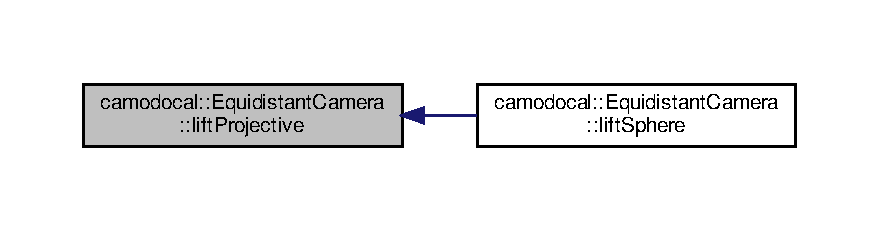
\includegraphics[width=350pt]{classcamodocal_1_1EquidistantCamera_accd38ebf90227cc221d91dad7dd57dbb_icgraph}
\end{center}
\end{figure}
\mbox{\Hypertarget{classcamodocal_1_1EquidistantCamera_ac86c8527e09b6df4eea4fd3c1322ba00}\label{classcamodocal_1_1EquidistantCamera_ac86c8527e09b6df4eea4fd3c1322ba00}} 
\index{camodocal\+::\+Equidistant\+Camera@{camodocal\+::\+Equidistant\+Camera}!lift\+Sphere@{lift\+Sphere}}
\index{lift\+Sphere@{lift\+Sphere}!camodocal\+::\+Equidistant\+Camera@{camodocal\+::\+Equidistant\+Camera}}
\subsubsection{\texorpdfstring{lift\+Sphere()}{liftSphere()}}
{\footnotesize\ttfamily void camodocal\+::\+Equidistant\+Camera\+::lift\+Sphere (\begin{DoxyParamCaption}\item[{const Eigen\+::\+Vector2d \&}]{p,  }\item[{Eigen\+::\+Vector3d \&}]{P }\end{DoxyParamCaption}) const\hspace{0.3cm}{\ttfamily [virtual]}}



Lifts a point from the image plane to the unit sphere. 


\begin{DoxyParams}{Parameters}
{\em p} & image coordinates \\
\hline
{\em P} & coordinates of the point on the sphere \\
\hline
\end{DoxyParams}


Implements \hyperlink{classcamodocal_1_1Camera_a77b4ea673c694741302efba6f86a0100}{camodocal\+::\+Camera}.



References lift\+Projective().

Here is the call graph for this function\+:\nopagebreak
\begin{figure}[H]
\begin{center}
\leavevmode
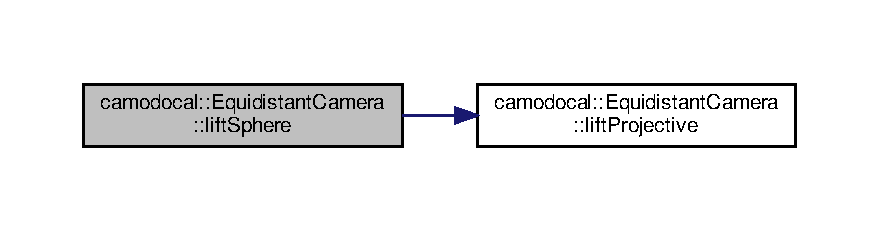
\includegraphics[width=350pt]{classcamodocal_1_1EquidistantCamera_ac86c8527e09b6df4eea4fd3c1322ba00_cgraph}
\end{center}
\end{figure}
\mbox{\Hypertarget{classcamodocal_1_1EquidistantCamera_a04de4daf1568c2425eabdbade499f927}\label{classcamodocal_1_1EquidistantCamera_a04de4daf1568c2425eabdbade499f927}} 
\index{camodocal\+::\+Equidistant\+Camera@{camodocal\+::\+Equidistant\+Camera}!space\+To\+Plane@{space\+To\+Plane}}
\index{space\+To\+Plane@{space\+To\+Plane}!camodocal\+::\+Equidistant\+Camera@{camodocal\+::\+Equidistant\+Camera}}
\subsubsection{\texorpdfstring{space\+To\+Plane()}{spaceToPlane()}\hspace{0.1cm}{\footnotesize\ttfamily [1/2]}}
{\footnotesize\ttfamily void camodocal\+::\+Equidistant\+Camera\+::space\+To\+Plane (\begin{DoxyParamCaption}\item[{const Eigen\+::\+Vector3d \&}]{P,  }\item[{Eigen\+::\+Vector2d \&}]{p }\end{DoxyParamCaption}) const\hspace{0.3cm}{\ttfamily [virtual]}}



Project a 3D point ({\itshape x},{\itshape y},{\itshape z}) to the image plane in ({\itshape u},{\itshape v}) 


\begin{DoxyParams}{Parameters}
{\em P} & 3D point coordinates \\
\hline
{\em p} & return value, contains the image point coordinates \\
\hline
\end{DoxyParams}


Implements \hyperlink{classcamodocal_1_1Camera_acf49bd1ef0919e0faf89d060dc497b52}{camodocal\+::\+Camera}.



Referenced by undist\+To\+Plane().

Here is the caller graph for this function\+:\nopagebreak
\begin{figure}[H]
\begin{center}
\leavevmode
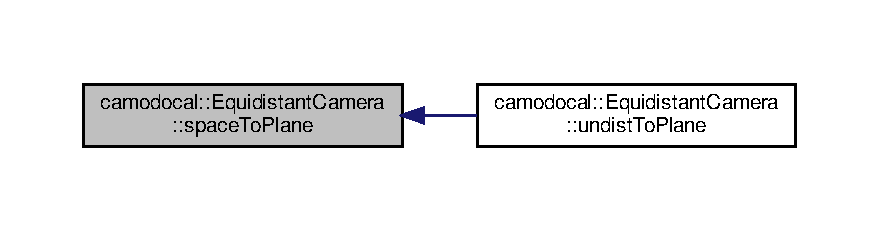
\includegraphics[width=350pt]{classcamodocal_1_1EquidistantCamera_a04de4daf1568c2425eabdbade499f927_icgraph}
\end{center}
\end{figure}
\mbox{\Hypertarget{classcamodocal_1_1EquidistantCamera_af24c481afa7e454a687fcdc7726d443f}\label{classcamodocal_1_1EquidistantCamera_af24c481afa7e454a687fcdc7726d443f}} 
\index{camodocal\+::\+Equidistant\+Camera@{camodocal\+::\+Equidistant\+Camera}!space\+To\+Plane@{space\+To\+Plane}}
\index{space\+To\+Plane@{space\+To\+Plane}!camodocal\+::\+Equidistant\+Camera@{camodocal\+::\+Equidistant\+Camera}}
\subsubsection{\texorpdfstring{space\+To\+Plane()}{spaceToPlane()}\hspace{0.1cm}{\footnotesize\ttfamily [2/2]}}
{\footnotesize\ttfamily void camodocal\+::\+Equidistant\+Camera\+::space\+To\+Plane (\begin{DoxyParamCaption}\item[{const Eigen\+::\+Vector3d \&}]{P,  }\item[{Eigen\+::\+Vector2d \&}]{p,  }\item[{Eigen\+::\+Matrix$<$ double, 2, 3 $>$ \&}]{J }\end{DoxyParamCaption}) const}



Project a 3D point to the image plane and calculate Jacobian. 


\begin{DoxyParams}{Parameters}
{\em P} & 3D point coordinates \\
\hline
{\em p} & return value, contains the image point coordinates \\
\hline
\end{DoxyParams}
\mbox{\Hypertarget{classcamodocal_1_1EquidistantCamera_ac0aae0a472fac59ad5fc22079eb5560d}\label{classcamodocal_1_1EquidistantCamera_ac0aae0a472fac59ad5fc22079eb5560d}} 
\index{camodocal\+::\+Equidistant\+Camera@{camodocal\+::\+Equidistant\+Camera}!undist\+To\+Plane@{undist\+To\+Plane}}
\index{undist\+To\+Plane@{undist\+To\+Plane}!camodocal\+::\+Equidistant\+Camera@{camodocal\+::\+Equidistant\+Camera}}
\subsubsection{\texorpdfstring{undist\+To\+Plane()}{undistToPlane()}}
{\footnotesize\ttfamily void camodocal\+::\+Equidistant\+Camera\+::undist\+To\+Plane (\begin{DoxyParamCaption}\item[{const Eigen\+::\+Vector2d \&}]{p\+\_\+u,  }\item[{Eigen\+::\+Vector2d \&}]{p }\end{DoxyParamCaption}) const\hspace{0.3cm}{\ttfamily [virtual]}}



Projects an undistorted 2D point p\+\_\+u to the image plane. 


\begin{DoxyParams}{Parameters}
{\em p\+\_\+u} & 2D point coordinates \\
\hline
\end{DoxyParams}
\begin{DoxyReturn}{Returns}
image point coordinates 
\end{DoxyReturn}


Implements \hyperlink{classcamodocal_1_1Camera}{camodocal\+::\+Camera}.



References camodocal\+::\+Camera\+::\+Parameters\+::image\+Height(), camodocal\+::\+Camera\+::\+Parameters\+::image\+Width(), and space\+To\+Plane().

Here is the call graph for this function\+:\nopagebreak
\begin{figure}[H]
\begin{center}
\leavevmode
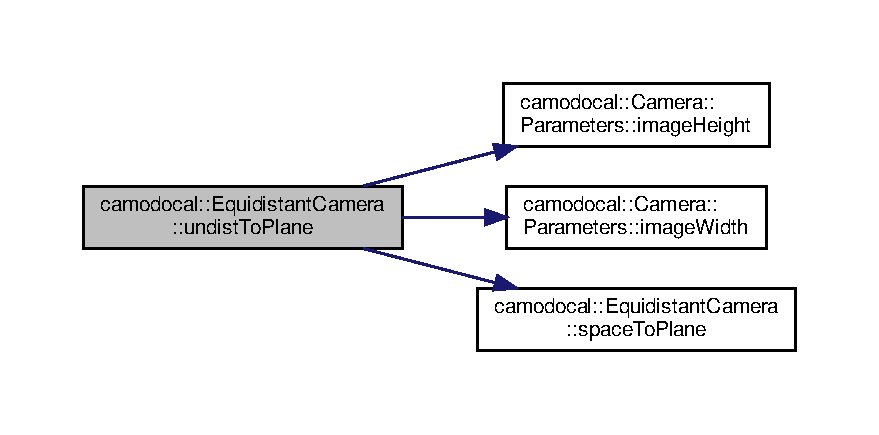
\includegraphics[width=350pt]{classcamodocal_1_1EquidistantCamera_ac0aae0a472fac59ad5fc22079eb5560d_cgraph}
\end{center}
\end{figure}


The documentation for this class was generated from the following files\+:\begin{DoxyCompactItemize}
\item 
camera\+\_\+model/include/camodocal/camera\+\_\+models/Equidistant\+Camera.\+h\item 
camera\+\_\+model/src/camera\+\_\+models/Equidistant\+Camera.\+cc\end{DoxyCompactItemize}

\hypertarget{classEstimator}{}\section{Estimator Class Reference}
\label{classEstimator}\index{Estimator@{Estimator}}


Collaboration diagram for Estimator\+:\nopagebreak
\begin{figure}[H]
\begin{center}
\leavevmode
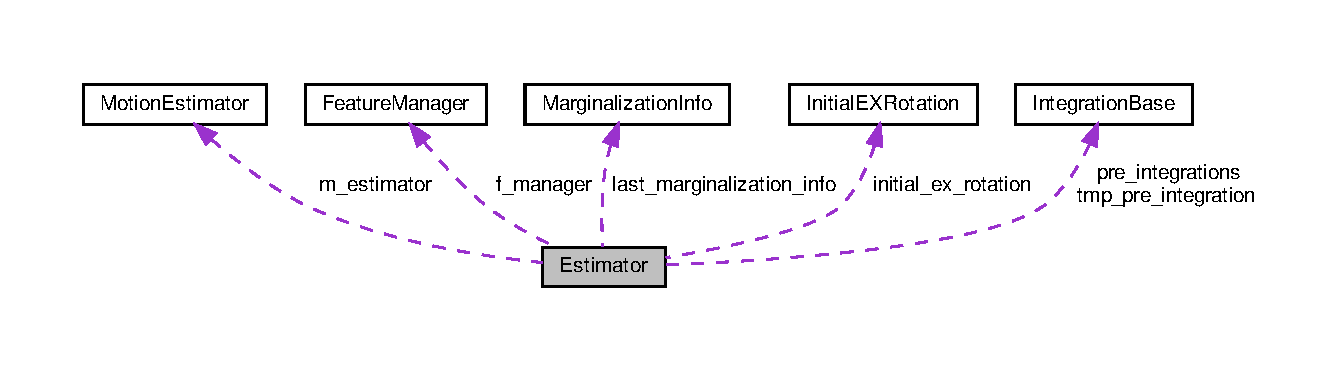
\includegraphics[width=350pt]{classEstimator__coll__graph}
\end{center}
\end{figure}
\subsection*{Public Types}
\begin{DoxyCompactItemize}
\item 
\mbox{\Hypertarget{classEstimator_ae4545de83f6d64233515112f7ff27628}\label{classEstimator_ae4545de83f6d64233515112f7ff27628}} 
enum {\bfseries Solver\+Flag} \{ {\bfseries I\+N\+I\+T\+I\+AL}, 
{\bfseries N\+O\+N\+\_\+\+L\+I\+N\+E\+AR}
 \}
\item 
\mbox{\Hypertarget{classEstimator_a020181ad0fe1f065d5ea8a4d414ce6b1}\label{classEstimator_a020181ad0fe1f065d5ea8a4d414ce6b1}} 
enum {\bfseries Marginalization\+Flag} \{ {\bfseries M\+A\+R\+G\+I\+N\+\_\+\+O\+LD} = 0, 
{\bfseries M\+A\+R\+G\+I\+N\+\_\+\+S\+E\+C\+O\+N\+D\+\_\+\+N\+EW} = 1
 \}
\end{DoxyCompactItemize}
\subsection*{Public Member Functions}
\begin{DoxyCompactItemize}
\item 
\mbox{\Hypertarget{classEstimator_a38f16d396fade5dee487db958d8f45da}\label{classEstimator_a38f16d396fade5dee487db958d8f45da}} 
void {\bfseries set\+Parameter} ()
\item 
void \hyperlink{classEstimator_aa44c20668ac637af041152abd568fe81}{process\+I\+MU} (double t, const Vector3d \&linear\+\_\+acceleration, const Vector3d \&angular\+\_\+velocity)
\begin{DoxyCompactList}\small\item\em processs I\+MU measurement \end{DoxyCompactList}\item 
void \hyperlink{classEstimator_aa6fb65bc801f80dc142e3a5f9d0109ee}{process\+Image} (const map$<$ int, vector$<$ pair$<$ int, Eigen\+::\+Matrix$<$ double, 7, 1 $>$$>$$>$$>$ \&image, const std\+\_\+msgs\+::\+Header \&header)
\begin{DoxyCompactList}\small\item\em process Image \end{DoxyCompactList}\item 
void \hyperlink{classEstimator_a13444b276377b490d799bad3a21c8bf9}{set\+Relo\+Frame} (double \+\_\+frame\+\_\+stamp, int \+\_\+frame\+\_\+index, vector$<$ Vector3d $>$ \&\+\_\+match\+\_\+points, Vector3d \+\_\+relo\+\_\+t, Matrix3d \+\_\+relo\+\_\+r)
\begin{DoxyCompactList}\small\item\em Set the Relo Frame object. \end{DoxyCompactList}\item 
\mbox{\Hypertarget{classEstimator_afd9366e076daf96e28a3b2b419a7b3ba}\label{classEstimator_afd9366e076daf96e28a3b2b419a7b3ba}} 
void {\bfseries clear\+State} ()
\item 
\mbox{\Hypertarget{classEstimator_a6da34743ac07ff0be15d58cfbe9ea9f1}\label{classEstimator_a6da34743ac07ff0be15d58cfbe9ea9f1}} 
bool {\bfseries initial\+Structure} ()
\item 
\mbox{\Hypertarget{classEstimator_af34f289f486b9d1e75ba83cae20980a7}\label{classEstimator_af34f289f486b9d1e75ba83cae20980a7}} 
bool {\bfseries visual\+Initial\+Align} ()
\item 
\mbox{\Hypertarget{classEstimator_a60ff51cc613465e06360f12966c7e1b5}\label{classEstimator_a60ff51cc613465e06360f12966c7e1b5}} 
bool {\bfseries relative\+Pose} (Matrix3d \&relative\+\_\+R, Vector3d \&relative\+\_\+T, int \&l)
\item 
\mbox{\Hypertarget{classEstimator_ac118df0372730107c7031489b26df117}\label{classEstimator_ac118df0372730107c7031489b26df117}} 
void {\bfseries slide\+Window} ()
\item 
\mbox{\Hypertarget{classEstimator_a6586d5b1a4d071f89e13c0a37e46d112}\label{classEstimator_a6586d5b1a4d071f89e13c0a37e46d112}} 
void {\bfseries solve\+Odometry} ()
\item 
\mbox{\Hypertarget{classEstimator_a6322c2277c69960554c7360ea3932360}\label{classEstimator_a6322c2277c69960554c7360ea3932360}} 
void {\bfseries slide\+Window\+New} ()
\item 
\mbox{\Hypertarget{classEstimator_a6763ef70f085dc18c36e3be425e015ca}\label{classEstimator_a6763ef70f085dc18c36e3be425e015ca}} 
void {\bfseries slide\+Window\+Old} ()
\item 
\mbox{\Hypertarget{classEstimator_a97efa571ccabe805e468ea8e497f86e3}\label{classEstimator_a97efa571ccabe805e468ea8e497f86e3}} 
void {\bfseries optimization} ()
\item 
\mbox{\Hypertarget{classEstimator_a7cef725addfe53cc17f929b7d303ca59}\label{classEstimator_a7cef725addfe53cc17f929b7d303ca59}} 
void {\bfseries vector2double} ()
\item 
\mbox{\Hypertarget{classEstimator_a1018d937f1596d05b7d9a8f119c5985a}\label{classEstimator_a1018d937f1596d05b7d9a8f119c5985a}} 
void {\bfseries double2vector} ()
\item 
\mbox{\Hypertarget{classEstimator_a9677152e40b9364ebc279c03ff932c56}\label{classEstimator_a9677152e40b9364ebc279c03ff932c56}} 
bool {\bfseries failure\+Detection} ()
\end{DoxyCompactItemize}
\subsection*{Public Attributes}
\begin{DoxyCompactItemize}
\item 
\mbox{\Hypertarget{classEstimator_a324ff7205fc2cce24547b6ff96e63271}\label{classEstimator_a324ff7205fc2cce24547b6ff96e63271}} 
Solver\+Flag {\bfseries solver\+\_\+flag}
\item 
\mbox{\Hypertarget{classEstimator_a4b22b2fb74b9118ff6732fc5342e5636}\label{classEstimator_a4b22b2fb74b9118ff6732fc5342e5636}} 
Marginalization\+Flag {\bfseries marginalization\+\_\+flag}
\item 
\mbox{\Hypertarget{classEstimator_aa47626f7b8776f9ddd8c9aec1f0a9921}\label{classEstimator_aa47626f7b8776f9ddd8c9aec1f0a9921}} 
Vector3d {\bfseries g}
\item 
\mbox{\Hypertarget{classEstimator_a2d641d68416a77576d1a23cc8d03beb4}\label{classEstimator_a2d641d68416a77576d1a23cc8d03beb4}} 
Matrix\+Xd {\bfseries Ap} \mbox{[}2\mbox{]}
\item 
\mbox{\Hypertarget{classEstimator_a2b5ba9e2978481957725122269513377}\label{classEstimator_a2b5ba9e2978481957725122269513377}} 
Matrix\+Xd {\bfseries backup\+\_\+A}
\item 
\mbox{\Hypertarget{classEstimator_ab06a60da062f5de4216b69cf10a972c3}\label{classEstimator_ab06a60da062f5de4216b69cf10a972c3}} 
Vector\+Xd {\bfseries bp} \mbox{[}2\mbox{]}
\item 
\mbox{\Hypertarget{classEstimator_a5d8208de33fb48e77d64e80c6ed7d159}\label{classEstimator_a5d8208de33fb48e77d64e80c6ed7d159}} 
Vector\+Xd {\bfseries backup\+\_\+b}
\item 
\mbox{\Hypertarget{classEstimator_aa2281c4dbc639434752ff72a63c143c5}\label{classEstimator_aa2281c4dbc639434752ff72a63c143c5}} 
Matrix3d {\bfseries ric} \mbox{[}N\+U\+M\+\_\+\+O\+F\+\_\+\+C\+AM\mbox{]}
\item 
\mbox{\Hypertarget{classEstimator_a2cc2a6796ea2f568543364fede9e1741}\label{classEstimator_a2cc2a6796ea2f568543364fede9e1741}} 
Vector3d {\bfseries tic} \mbox{[}N\+U\+M\+\_\+\+O\+F\+\_\+\+C\+AM\mbox{]}
\item 
\mbox{\Hypertarget{classEstimator_ae39aafb5802c16f66b9b478861c05214}\label{classEstimator_ae39aafb5802c16f66b9b478861c05214}} 
Vector3d {\bfseries Ps} \mbox{[}(W\+I\+N\+D\+O\+W\+\_\+\+S\+I\+ZE+1)\mbox{]}
\item 
\mbox{\Hypertarget{classEstimator_a261ce91e7dbfb155d52c09daf1a81f4e}\label{classEstimator_a261ce91e7dbfb155d52c09daf1a81f4e}} 
Vector3d {\bfseries Vs} \mbox{[}(W\+I\+N\+D\+O\+W\+\_\+\+S\+I\+ZE+1)\mbox{]}
\item 
\mbox{\Hypertarget{classEstimator_a95fb17a6e27d168aeecfea6debc5b654}\label{classEstimator_a95fb17a6e27d168aeecfea6debc5b654}} 
Matrix3d {\bfseries Rs} \mbox{[}(W\+I\+N\+D\+O\+W\+\_\+\+S\+I\+ZE+1)\mbox{]}
\item 
\mbox{\Hypertarget{classEstimator_ab37b75b88457b47d77cb98d98c84313b}\label{classEstimator_ab37b75b88457b47d77cb98d98c84313b}} 
Vector3d {\bfseries Bas} \mbox{[}(W\+I\+N\+D\+O\+W\+\_\+\+S\+I\+ZE+1)\mbox{]}
\item 
\mbox{\Hypertarget{classEstimator_a75bcfcfcd62b388231812b7cf54d0609}\label{classEstimator_a75bcfcfcd62b388231812b7cf54d0609}} 
Vector3d {\bfseries Bgs} \mbox{[}(W\+I\+N\+D\+O\+W\+\_\+\+S\+I\+ZE+1)\mbox{]}
\item 
\mbox{\Hypertarget{classEstimator_af5af4dd3209c9bb1cac39b28ca13ef9e}\label{classEstimator_af5af4dd3209c9bb1cac39b28ca13ef9e}} 
double {\bfseries td}
\item 
\mbox{\Hypertarget{classEstimator_ae25ec3c331182aa10cf93062a0013462}\label{classEstimator_ae25ec3c331182aa10cf93062a0013462}} 
Matrix3d {\bfseries back\+\_\+\+R0}
\item 
\mbox{\Hypertarget{classEstimator_ae767a1f8631b2e48cdd2f5a5f94af4f8}\label{classEstimator_ae767a1f8631b2e48cdd2f5a5f94af4f8}} 
Matrix3d {\bfseries last\+\_\+R}
\item 
\mbox{\Hypertarget{classEstimator_ad66c36afc29ed73dae943d7dbb93339c}\label{classEstimator_ad66c36afc29ed73dae943d7dbb93339c}} 
Matrix3d {\bfseries last\+\_\+\+R0}
\item 
\mbox{\Hypertarget{classEstimator_a488253ad9835484585df51adde8f4bb8}\label{classEstimator_a488253ad9835484585df51adde8f4bb8}} 
Vector3d {\bfseries back\+\_\+\+P0}
\item 
\mbox{\Hypertarget{classEstimator_a3c69cfe5a1b003eb19c4869e3db6b7d7}\label{classEstimator_a3c69cfe5a1b003eb19c4869e3db6b7d7}} 
Vector3d {\bfseries last\+\_\+P}
\item 
\mbox{\Hypertarget{classEstimator_a7739a4e119a156d5c544072289bfbad2}\label{classEstimator_a7739a4e119a156d5c544072289bfbad2}} 
Vector3d {\bfseries last\+\_\+\+P0}
\item 
\mbox{\Hypertarget{classEstimator_ab0dfabed3a2b43af2edbb27034c00837}\label{classEstimator_ab0dfabed3a2b43af2edbb27034c00837}} 
std\+\_\+msgs\+::\+Header {\bfseries Headers} \mbox{[}(W\+I\+N\+D\+O\+W\+\_\+\+S\+I\+ZE+1)\mbox{]}
\item 
\mbox{\Hypertarget{classEstimator_ad4eda10e539c70aa084b2c12b3f2a91e}\label{classEstimator_ad4eda10e539c70aa084b2c12b3f2a91e}} 
\hyperlink{classIntegrationBase}{Integration\+Base} $\ast$ {\bfseries pre\+\_\+integrations} \mbox{[}(W\+I\+N\+D\+O\+W\+\_\+\+S\+I\+ZE+1)\mbox{]}
\item 
\mbox{\Hypertarget{classEstimator_aaf838ba54ec51344bdb46ab8fed5a31a}\label{classEstimator_aaf838ba54ec51344bdb46ab8fed5a31a}} 
Vector3d {\bfseries acc\+\_\+0}
\item 
\mbox{\Hypertarget{classEstimator_ab100397542d96248fd4e96cdcb5c7b6a}\label{classEstimator_ab100397542d96248fd4e96cdcb5c7b6a}} 
Vector3d {\bfseries gyr\+\_\+0}
\item 
\mbox{\Hypertarget{classEstimator_a844443a999600e2627f7486ea28a5eb6}\label{classEstimator_a844443a999600e2627f7486ea28a5eb6}} 
vector$<$ double $>$ {\bfseries dt\+\_\+buf} \mbox{[}(W\+I\+N\+D\+O\+W\+\_\+\+S\+I\+ZE+1)\mbox{]}
\item 
\mbox{\Hypertarget{classEstimator_aaae7dad254aba40dc261f29ae985fa9d}\label{classEstimator_aaae7dad254aba40dc261f29ae985fa9d}} 
vector$<$ Vector3d $>$ {\bfseries linear\+\_\+acceleration\+\_\+buf} \mbox{[}(W\+I\+N\+D\+O\+W\+\_\+\+S\+I\+ZE+1)\mbox{]}
\item 
\mbox{\Hypertarget{classEstimator_a653b46f9a739aa16ab0d2da59b747ba1}\label{classEstimator_a653b46f9a739aa16ab0d2da59b747ba1}} 
vector$<$ Vector3d $>$ {\bfseries angular\+\_\+velocity\+\_\+buf} \mbox{[}(W\+I\+N\+D\+O\+W\+\_\+\+S\+I\+ZE+1)\mbox{]}
\item 
\mbox{\Hypertarget{classEstimator_add0682c516a2c046091eb78fb66a074b}\label{classEstimator_add0682c516a2c046091eb78fb66a074b}} 
int {\bfseries frame\+\_\+count}
\item 
\mbox{\Hypertarget{classEstimator_a687dfa6523f8b161a58d364981fc89d6}\label{classEstimator_a687dfa6523f8b161a58d364981fc89d6}} 
int {\bfseries sum\+\_\+of\+\_\+outlier}
\item 
\mbox{\Hypertarget{classEstimator_a9373c8ca8fa2f85429c533a9e962cac9}\label{classEstimator_a9373c8ca8fa2f85429c533a9e962cac9}} 
int {\bfseries sum\+\_\+of\+\_\+back}
\item 
\mbox{\Hypertarget{classEstimator_a116e4d7566f6085634a1b584a969e1d6}\label{classEstimator_a116e4d7566f6085634a1b584a969e1d6}} 
int {\bfseries sum\+\_\+of\+\_\+front}
\item 
\mbox{\Hypertarget{classEstimator_a995855d093897b972fc2f6197c4691be}\label{classEstimator_a995855d093897b972fc2f6197c4691be}} 
int {\bfseries sum\+\_\+of\+\_\+invalid}
\item 
\mbox{\Hypertarget{classEstimator_a538a896b46287ec27eb8bf2b9f9efbdb}\label{classEstimator_a538a896b46287ec27eb8bf2b9f9efbdb}} 
\hyperlink{classFeatureManager}{Feature\+Manager} {\bfseries f\+\_\+manager}
\item 
\mbox{\Hypertarget{classEstimator_aec88a9bb2c79e1b1f3f9132250e1758c}\label{classEstimator_aec88a9bb2c79e1b1f3f9132250e1758c}} 
\hyperlink{classMotionEstimator}{Motion\+Estimator} {\bfseries m\+\_\+estimator}
\item 
\mbox{\Hypertarget{classEstimator_a8fc923bb45f8bfe6419d54c6dd34c8f5}\label{classEstimator_a8fc923bb45f8bfe6419d54c6dd34c8f5}} 
\hyperlink{classInitialEXRotation}{Initial\+E\+X\+Rotation} {\bfseries initial\+\_\+ex\+\_\+rotation}
\item 
\mbox{\Hypertarget{classEstimator_afc50690d3bca730204f82d445bb54595}\label{classEstimator_afc50690d3bca730204f82d445bb54595}} 
bool {\bfseries first\+\_\+imu}
\item 
\mbox{\Hypertarget{classEstimator_acbc6a7508fbfd8fd6fef84b265c4b997}\label{classEstimator_acbc6a7508fbfd8fd6fef84b265c4b997}} 
bool {\bfseries is\+\_\+valid}
\item 
\mbox{\Hypertarget{classEstimator_aee5ac9e3fc04d1d8b4fa21f9265529d1}\label{classEstimator_aee5ac9e3fc04d1d8b4fa21f9265529d1}} 
bool {\bfseries is\+\_\+key}
\item 
\mbox{\Hypertarget{classEstimator_aaa1373cca2384c09ec5569040d57949b}\label{classEstimator_aaa1373cca2384c09ec5569040d57949b}} 
bool {\bfseries failure\+\_\+occur}
\item 
\mbox{\Hypertarget{classEstimator_aaffeb52bc8eb64345b171316fd45d08f}\label{classEstimator_aaffeb52bc8eb64345b171316fd45d08f}} 
vector$<$ Vector3d $>$ {\bfseries point\+\_\+cloud}
\item 
\mbox{\Hypertarget{classEstimator_a1fe1c936d5316a4b9730b2a2c4f8d1e6}\label{classEstimator_a1fe1c936d5316a4b9730b2a2c4f8d1e6}} 
vector$<$ Vector3d $>$ {\bfseries margin\+\_\+cloud}
\item 
\mbox{\Hypertarget{classEstimator_a2366a415eb299d9c0dafaf685e64ab5d}\label{classEstimator_a2366a415eb299d9c0dafaf685e64ab5d}} 
vector$<$ Vector3d $>$ {\bfseries key\+\_\+poses}
\item 
\mbox{\Hypertarget{classEstimator_af16e6493e5161056a25669fabbcc94e7}\label{classEstimator_af16e6493e5161056a25669fabbcc94e7}} 
double {\bfseries initial\+\_\+timestamp}
\item 
\mbox{\Hypertarget{classEstimator_a784461c0ec721136a5e81280320464ca}\label{classEstimator_a784461c0ec721136a5e81280320464ca}} 
double {\bfseries para\+\_\+\+Pose} \mbox{[}W\+I\+N\+D\+O\+W\+\_\+\+S\+I\+ZE+1\mbox{]}\mbox{[}S\+I\+Z\+E\+\_\+\+P\+O\+SE\mbox{]}
\item 
\mbox{\Hypertarget{classEstimator_aeb6a30336a78f219f0ae9b40ae30d4b9}\label{classEstimator_aeb6a30336a78f219f0ae9b40ae30d4b9}} 
double {\bfseries para\+\_\+\+Speed\+Bias} \mbox{[}W\+I\+N\+D\+O\+W\+\_\+\+S\+I\+ZE+1\mbox{]}\mbox{[}S\+I\+Z\+E\+\_\+\+S\+P\+E\+E\+D\+B\+I\+AS\mbox{]}
\item 
\mbox{\Hypertarget{classEstimator_aeca39f6e3a06edf52e113840e2abe69b}\label{classEstimator_aeca39f6e3a06edf52e113840e2abe69b}} 
double {\bfseries para\+\_\+\+Feature} \mbox{[}N\+U\+M\+\_\+\+O\+F\+\_\+F\mbox{]}\mbox{[}S\+I\+Z\+E\+\_\+\+F\+E\+A\+T\+U\+RE\mbox{]}
\item 
\mbox{\Hypertarget{classEstimator_aebc1cb85071d7c6849865e4d20a02780}\label{classEstimator_aebc1cb85071d7c6849865e4d20a02780}} 
double {\bfseries para\+\_\+\+Ex\+\_\+\+Pose} \mbox{[}N\+U\+M\+\_\+\+O\+F\+\_\+\+C\+AM\mbox{]}\mbox{[}S\+I\+Z\+E\+\_\+\+P\+O\+SE\mbox{]}
\item 
\mbox{\Hypertarget{classEstimator_a0ec701cfdc86b7b48734a0a26731187e}\label{classEstimator_a0ec701cfdc86b7b48734a0a26731187e}} 
double {\bfseries para\+\_\+\+Retrive\+\_\+\+Pose} \mbox{[}S\+I\+Z\+E\+\_\+\+P\+O\+SE\mbox{]}
\item 
\mbox{\Hypertarget{classEstimator_a19f645fa7edf6b47ad0737300112077a}\label{classEstimator_a19f645fa7edf6b47ad0737300112077a}} 
double {\bfseries para\+\_\+\+Td} \mbox{[}1\mbox{]}\mbox{[}1\mbox{]}
\item 
\mbox{\Hypertarget{classEstimator_abe559fb7fa6553c83cc3813a51ce289e}\label{classEstimator_abe559fb7fa6553c83cc3813a51ce289e}} 
double {\bfseries para\+\_\+\+Tr} \mbox{[}1\mbox{]}\mbox{[}1\mbox{]}
\item 
\mbox{\Hypertarget{classEstimator_aede01f278966422211ea9996b62b54d8}\label{classEstimator_aede01f278966422211ea9996b62b54d8}} 
int {\bfseries loop\+\_\+window\+\_\+index}
\item 
\mbox{\Hypertarget{classEstimator_ada21a832baba2ed43a09d025a73b1086}\label{classEstimator_ada21a832baba2ed43a09d025a73b1086}} 
\hyperlink{classMarginalizationInfo}{Marginalization\+Info} $\ast$ {\bfseries last\+\_\+marginalization\+\_\+info}
\item 
\mbox{\Hypertarget{classEstimator_ac8e1ca84050653626b3a0850be59e344}\label{classEstimator_ac8e1ca84050653626b3a0850be59e344}} 
vector$<$ double $\ast$ $>$ {\bfseries last\+\_\+marginalization\+\_\+parameter\+\_\+blocks}
\item 
\mbox{\Hypertarget{classEstimator_ad6a31a9049e505fb4c17ff95211d5531}\label{classEstimator_ad6a31a9049e505fb4c17ff95211d5531}} 
map$<$ double, \hyperlink{classImageFrame}{Image\+Frame} $>$ {\bfseries all\+\_\+image\+\_\+frame}
\item 
\mbox{\Hypertarget{classEstimator_aec37f5a60f299724b6b796969fa765f4}\label{classEstimator_aec37f5a60f299724b6b796969fa765f4}} 
\hyperlink{classIntegrationBase}{Integration\+Base} $\ast$ {\bfseries tmp\+\_\+pre\+\_\+integration}
\item 
\mbox{\Hypertarget{classEstimator_ac40e539f316194131ffe2bf082f82537}\label{classEstimator_ac40e539f316194131ffe2bf082f82537}} 
bool {\bfseries relocalization\+\_\+info}
\item 
\mbox{\Hypertarget{classEstimator_a72bb067de7c931a12676bd2730f55f35}\label{classEstimator_a72bb067de7c931a12676bd2730f55f35}} 
double {\bfseries relo\+\_\+frame\+\_\+stamp}
\item 
\mbox{\Hypertarget{classEstimator_a086049606f6010d07fa9784b87b2b8cf}\label{classEstimator_a086049606f6010d07fa9784b87b2b8cf}} 
double {\bfseries relo\+\_\+frame\+\_\+index}
\item 
\mbox{\Hypertarget{classEstimator_aefda23319479cd02fc65f1868a4c6563}\label{classEstimator_aefda23319479cd02fc65f1868a4c6563}} 
int {\bfseries relo\+\_\+frame\+\_\+local\+\_\+index}
\item 
\mbox{\Hypertarget{classEstimator_aaaef771460da95bd973293e9d7b07678}\label{classEstimator_aaaef771460da95bd973293e9d7b07678}} 
vector$<$ Vector3d $>$ {\bfseries match\+\_\+points}
\item 
\mbox{\Hypertarget{classEstimator_a00de2e0216cf87c7b5d65c49fec4cf3c}\label{classEstimator_a00de2e0216cf87c7b5d65c49fec4cf3c}} 
double {\bfseries relo\+\_\+\+Pose} \mbox{[}S\+I\+Z\+E\+\_\+\+P\+O\+SE\mbox{]}
\item 
\mbox{\Hypertarget{classEstimator_af6f0798d2af603a09c33efae290e1ec3}\label{classEstimator_af6f0798d2af603a09c33efae290e1ec3}} 
Matrix3d {\bfseries drift\+\_\+correct\+\_\+r}
\item 
\mbox{\Hypertarget{classEstimator_a922567580fbaaa68dc90a7baa06ec32b}\label{classEstimator_a922567580fbaaa68dc90a7baa06ec32b}} 
Vector3d {\bfseries drift\+\_\+correct\+\_\+t}
\item 
\mbox{\Hypertarget{classEstimator_ac847ec23a5024ebbb3a73f3721ee3e47}\label{classEstimator_ac847ec23a5024ebbb3a73f3721ee3e47}} 
Vector3d {\bfseries prev\+\_\+relo\+\_\+t}
\item 
\mbox{\Hypertarget{classEstimator_ad5c0584ee27e037a3a4378a73739c309}\label{classEstimator_ad5c0584ee27e037a3a4378a73739c309}} 
Matrix3d {\bfseries prev\+\_\+relo\+\_\+r}
\item 
\mbox{\Hypertarget{classEstimator_ace6808815c79b92f2a818748e31f3e8b}\label{classEstimator_ace6808815c79b92f2a818748e31f3e8b}} 
Vector3d {\bfseries relo\+\_\+relative\+\_\+t}
\item 
\mbox{\Hypertarget{classEstimator_a5d360d01f5f76bcf1a45ba7b98eda2d4}\label{classEstimator_a5d360d01f5f76bcf1a45ba7b98eda2d4}} 
Quaterniond {\bfseries relo\+\_\+relative\+\_\+q}
\item 
\mbox{\Hypertarget{classEstimator_afc85fb295cdd4ec9bd851b4f4a591bdd}\label{classEstimator_afc85fb295cdd4ec9bd851b4f4a591bdd}} 
double {\bfseries relo\+\_\+relative\+\_\+yaw}
\end{DoxyCompactItemize}


\subsection{Member Function Documentation}
\mbox{\Hypertarget{classEstimator_aa6fb65bc801f80dc142e3a5f9d0109ee}\label{classEstimator_aa6fb65bc801f80dc142e3a5f9d0109ee}} 
\index{Estimator@{Estimator}!process\+Image@{process\+Image}}
\index{process\+Image@{process\+Image}!Estimator@{Estimator}}
\subsubsection{\texorpdfstring{process\+Image()}{processImage()}}
{\footnotesize\ttfamily void Estimator\+::process\+Image (\begin{DoxyParamCaption}\item[{const map$<$ int, vector$<$ pair$<$ int, Eigen\+::\+Matrix$<$ double, 7, 1 $>$$>$$>$$>$ \&}]{image,  }\item[{const std\+\_\+msgs\+::\+Header \&}]{header }\end{DoxyParamCaption})}



process Image 


\begin{DoxyParams}{Parameters}
{\em image} & \\
\hline
{\em header} & \\
\hline
\end{DoxyParams}


References Global\+S\+F\+M\+::construct(), S\+F\+M\+Feature\+::id, and S\+F\+M\+Feature\+::observation.

Here is the call graph for this function\+:
\nopagebreak
\begin{figure}[H]
\begin{center}
\leavevmode
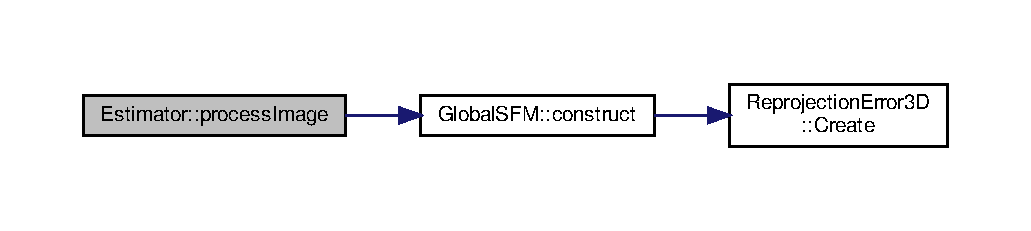
\includegraphics[width=350pt]{classEstimator_aa6fb65bc801f80dc142e3a5f9d0109ee_cgraph}
\end{center}
\end{figure}
\mbox{\Hypertarget{classEstimator_aa44c20668ac637af041152abd568fe81}\label{classEstimator_aa44c20668ac637af041152abd568fe81}} 
\index{Estimator@{Estimator}!process\+I\+MU@{process\+I\+MU}}
\index{process\+I\+MU@{process\+I\+MU}!Estimator@{Estimator}}
\subsubsection{\texorpdfstring{process\+I\+M\+U()}{processIMU()}}
{\footnotesize\ttfamily void Estimator\+::process\+I\+MU (\begin{DoxyParamCaption}\item[{double}]{t,  }\item[{const Vector3d \&}]{linear\+\_\+acceleration,  }\item[{const Vector3d \&}]{angular\+\_\+velocity }\end{DoxyParamCaption})}



processs I\+MU measurement 


\begin{DoxyParams}{Parameters}
{\em t} & \\
\hline
{\em linear\+\_\+acceleration} & \\
\hline
{\em angular\+\_\+velocity} & \\
\hline
\end{DoxyParams}
\mbox{\Hypertarget{classEstimator_a13444b276377b490d799bad3a21c8bf9}\label{classEstimator_a13444b276377b490d799bad3a21c8bf9}} 
\index{Estimator@{Estimator}!set\+Relo\+Frame@{set\+Relo\+Frame}}
\index{set\+Relo\+Frame@{set\+Relo\+Frame}!Estimator@{Estimator}}
\subsubsection{\texorpdfstring{set\+Relo\+Frame()}{setReloFrame()}}
{\footnotesize\ttfamily void Estimator\+::set\+Relo\+Frame (\begin{DoxyParamCaption}\item[{double}]{\+\_\+frame\+\_\+stamp,  }\item[{int}]{\+\_\+frame\+\_\+index,  }\item[{vector$<$ Vector3d $>$ \&}]{\+\_\+match\+\_\+points,  }\item[{Vector3d}]{\+\_\+relo\+\_\+t,  }\item[{Matrix3d}]{\+\_\+relo\+\_\+r }\end{DoxyParamCaption})}



Set the Relo Frame object. 


\begin{DoxyParams}{Parameters}
{\em \+\_\+frame\+\_\+stamp} & \\
\hline
{\em \+\_\+frame\+\_\+index} & \\
\hline
{\em \+\_\+match\+\_\+points} & \\
\hline
{\em \+\_\+relo\+\_\+t} & \\
\hline
{\em \+\_\+relo\+\_\+r} & \\
\hline
\end{DoxyParams}


The documentation for this class was generated from the following files\+:\begin{DoxyCompactItemize}
\item 
vins\+\_\+estimator/src/estimator.\+h\item 
vins\+\_\+estimator/src/estimator.\+cpp\end{DoxyCompactItemize}

\hypertarget{classDBoW2_1_1FBrief}{}\section{D\+Bo\+W2\+:\+:F\+Brief Class Reference}
\label{classDBoW2_1_1FBrief}\index{D\+Bo\+W2\+::\+F\+Brief@{D\+Bo\+W2\+::\+F\+Brief}}


Functions to manipulate B\+R\+I\+EF descriptors.  




{\ttfamily \#include $<$F\+Brief.\+h$>$}



Inheritance diagram for D\+Bo\+W2\+:\+:F\+Brief\+:\nopagebreak
\begin{figure}[H]
\begin{center}
\leavevmode
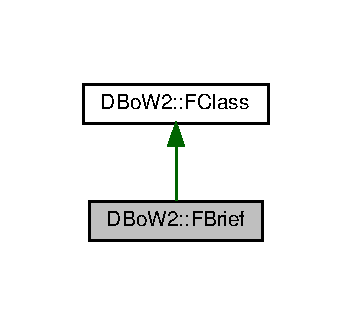
\includegraphics[width=169pt]{classDBoW2_1_1FBrief__inherit__graph}
\end{center}
\end{figure}


Collaboration diagram for D\+Bo\+W2\+:\+:F\+Brief\+:\nopagebreak
\begin{figure}[H]
\begin{center}
\leavevmode
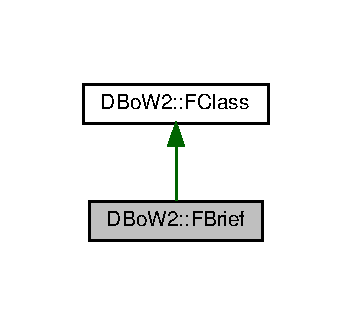
\includegraphics[width=169pt]{classDBoW2_1_1FBrief__coll__graph}
\end{center}
\end{figure}
\subsection*{Public Types}
\begin{DoxyCompactItemize}
\item 
\mbox{\Hypertarget{classDBoW2_1_1FBrief_acd27683ebe8fa8f482bf49f006930981}\label{classDBoW2_1_1FBrief_acd27683ebe8fa8f482bf49f006930981}} 
typedef \hyperlink{classDVision_1_1BRIEF_abc56a095174a93b0741099f35230b7c5}{D\+Vision\+::\+B\+R\+I\+E\+F\+::bitset} {\bfseries T\+Descriptor}
\item 
\mbox{\Hypertarget{classDBoW2_1_1FBrief_af7752017bb05cdac90a31491d701bb43}\label{classDBoW2_1_1FBrief_af7752017bb05cdac90a31491d701bb43}} 
typedef const T\+Descriptor $\ast$ {\bfseries p\+Descriptor}
\end{DoxyCompactItemize}
\subsection*{Static Public Member Functions}
\begin{DoxyCompactItemize}
\item 
static void \hyperlink{classDBoW2_1_1FBrief_a2808910daf6af046b47925715d71b564}{mean\+Value} (const std\+::vector$<$ p\+Descriptor $>$ \&descriptors, T\+Descriptor \&mean)
\item 
static double \hyperlink{classDBoW2_1_1FBrief_adc1c516cc0a2c9847853653956e8c35a}{distance} (const T\+Descriptor \&a, const T\+Descriptor \&b)
\item 
static std\+::string \hyperlink{classDBoW2_1_1FBrief_a271da94381cfb7a39664e5fc1d32a476}{to\+String} (const T\+Descriptor \&a)
\item 
static void \hyperlink{classDBoW2_1_1FBrief_a05bb35b06cc95b41edc80640ef2ea9f5}{from\+String} (T\+Descriptor \&a, const std\+::string \&s)
\item 
static void \hyperlink{classDBoW2_1_1FBrief_a626d885be78dfe839083b2ffb220150d}{to\+Mat32F} (const std\+::vector$<$ T\+Descriptor $>$ \&descriptors, cv\+::\+Mat \&mat)
\end{DoxyCompactItemize}


\subsection{Detailed Description}
Functions to manipulate B\+R\+I\+EF descriptors. 

\subsection{Member Function Documentation}
\mbox{\Hypertarget{classDBoW2_1_1FBrief_adc1c516cc0a2c9847853653956e8c35a}\label{classDBoW2_1_1FBrief_adc1c516cc0a2c9847853653956e8c35a}} 
\index{D\+Bo\+W2\+::\+F\+Brief@{D\+Bo\+W2\+::\+F\+Brief}!distance@{distance}}
\index{distance@{distance}!D\+Bo\+W2\+::\+F\+Brief@{D\+Bo\+W2\+::\+F\+Brief}}
\subsubsection{\texorpdfstring{distance()}{distance()}}
{\footnotesize\ttfamily double D\+Bo\+W2\+::\+F\+Brief\+::distance (\begin{DoxyParamCaption}\item[{const T\+Descriptor \&}]{a,  }\item[{const T\+Descriptor \&}]{b }\end{DoxyParamCaption})\hspace{0.3cm}{\ttfamily [static]}}

Calculates the distance between two descriptors 
\begin{DoxyParams}{Parameters}
{\em a} & \\
\hline
{\em b} & \\
\hline
\end{DoxyParams}
\begin{DoxyReturn}{Returns}
distance 
\end{DoxyReturn}


References D\+Vision\+::\+B\+R\+I\+E\+F\+::distance().

Here is the call graph for this function\+:\nopagebreak
\begin{figure}[H]
\begin{center}
\leavevmode
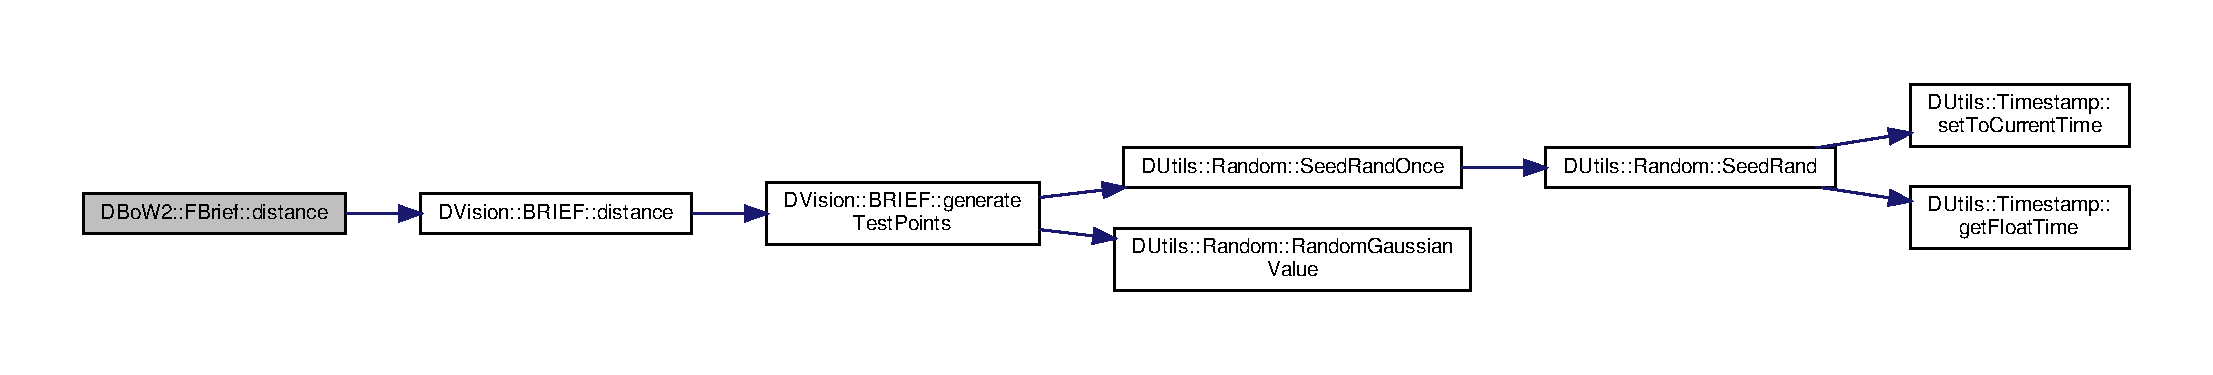
\includegraphics[width=350pt]{classDBoW2_1_1FBrief_adc1c516cc0a2c9847853653956e8c35a_cgraph}
\end{center}
\end{figure}
\mbox{\Hypertarget{classDBoW2_1_1FBrief_a05bb35b06cc95b41edc80640ef2ea9f5}\label{classDBoW2_1_1FBrief_a05bb35b06cc95b41edc80640ef2ea9f5}} 
\index{D\+Bo\+W2\+::\+F\+Brief@{D\+Bo\+W2\+::\+F\+Brief}!from\+String@{from\+String}}
\index{from\+String@{from\+String}!D\+Bo\+W2\+::\+F\+Brief@{D\+Bo\+W2\+::\+F\+Brief}}
\subsubsection{\texorpdfstring{from\+String()}{fromString()}}
{\footnotesize\ttfamily void D\+Bo\+W2\+::\+F\+Brief\+::from\+String (\begin{DoxyParamCaption}\item[{F\+Brief\+::\+T\+Descriptor \&}]{a,  }\item[{const std\+::string \&}]{s }\end{DoxyParamCaption})\hspace{0.3cm}{\ttfamily [static]}}

Returns a descriptor from a string 
\begin{DoxyParams}{Parameters}
{\em a} & descriptor \\
\hline
{\em s} & string version \\
\hline
\end{DoxyParams}
\mbox{\Hypertarget{classDBoW2_1_1FBrief_a2808910daf6af046b47925715d71b564}\label{classDBoW2_1_1FBrief_a2808910daf6af046b47925715d71b564}} 
\index{D\+Bo\+W2\+::\+F\+Brief@{D\+Bo\+W2\+::\+F\+Brief}!mean\+Value@{mean\+Value}}
\index{mean\+Value@{mean\+Value}!D\+Bo\+W2\+::\+F\+Brief@{D\+Bo\+W2\+::\+F\+Brief}}
\subsubsection{\texorpdfstring{mean\+Value()}{meanValue()}}
{\footnotesize\ttfamily void D\+Bo\+W2\+::\+F\+Brief\+::mean\+Value (\begin{DoxyParamCaption}\item[{const std\+::vector$<$ p\+Descriptor $>$ \&}]{descriptors,  }\item[{F\+Brief\+::\+T\+Descriptor \&}]{mean }\end{DoxyParamCaption})\hspace{0.3cm}{\ttfamily [static]}}

Calculates the mean value of a set of descriptors 
\begin{DoxyParams}{Parameters}
{\em descriptors} & \\
\hline
{\em mean} & mean descriptor \\
\hline
\end{DoxyParams}
\mbox{\Hypertarget{classDBoW2_1_1FBrief_a626d885be78dfe839083b2ffb220150d}\label{classDBoW2_1_1FBrief_a626d885be78dfe839083b2ffb220150d}} 
\index{D\+Bo\+W2\+::\+F\+Brief@{D\+Bo\+W2\+::\+F\+Brief}!to\+Mat32F@{to\+Mat32F}}
\index{to\+Mat32F@{to\+Mat32F}!D\+Bo\+W2\+::\+F\+Brief@{D\+Bo\+W2\+::\+F\+Brief}}
\subsubsection{\texorpdfstring{to\+Mat32\+F()}{toMat32F()}}
{\footnotesize\ttfamily void D\+Bo\+W2\+::\+F\+Brief\+::to\+Mat32F (\begin{DoxyParamCaption}\item[{const std\+::vector$<$ T\+Descriptor $>$ \&}]{descriptors,  }\item[{cv\+::\+Mat \&}]{mat }\end{DoxyParamCaption})\hspace{0.3cm}{\ttfamily [static]}}

Returns a mat with the descriptors in float format 
\begin{DoxyParams}{Parameters}
{\em descriptors} & \\
\hline
{\em mat} & (out) NxL 32F matrix \\
\hline
\end{DoxyParams}
\mbox{\Hypertarget{classDBoW2_1_1FBrief_a271da94381cfb7a39664e5fc1d32a476}\label{classDBoW2_1_1FBrief_a271da94381cfb7a39664e5fc1d32a476}} 
\index{D\+Bo\+W2\+::\+F\+Brief@{D\+Bo\+W2\+::\+F\+Brief}!to\+String@{to\+String}}
\index{to\+String@{to\+String}!D\+Bo\+W2\+::\+F\+Brief@{D\+Bo\+W2\+::\+F\+Brief}}
\subsubsection{\texorpdfstring{to\+String()}{toString()}}
{\footnotesize\ttfamily std\+::string D\+Bo\+W2\+::\+F\+Brief\+::to\+String (\begin{DoxyParamCaption}\item[{const T\+Descriptor \&}]{a }\end{DoxyParamCaption})\hspace{0.3cm}{\ttfamily [static]}}

Returns a string version of the descriptor 
\begin{DoxyParams}{Parameters}
{\em a} & descriptor \\
\hline
\end{DoxyParams}
\begin{DoxyReturn}{Returns}
string version 
\end{DoxyReturn}


The documentation for this class was generated from the following files\+:\begin{DoxyCompactItemize}
\item 
pose\+\_\+graph/src/\+Third\+Party/\+D\+Bo\+W/F\+Brief.\+h\item 
pose\+\_\+graph/src/\+Third\+Party/\+D\+Bo\+W/F\+Brief.\+cpp\end{DoxyCompactItemize}

\hypertarget{classDBoW2_1_1FClass}{}\section{D\+Bo\+W2\+:\+:F\+Class Class Reference}
\label{classDBoW2_1_1FClass}\index{D\+Bo\+W2\+::\+F\+Class@{D\+Bo\+W2\+::\+F\+Class}}


Generic class to encapsulate functions to manage descriptors.  




{\ttfamily \#include $<$F\+Class.\+h$>$}



Inheritance diagram for D\+Bo\+W2\+:\+:F\+Class\+:\nopagebreak
\begin{figure}[H]
\begin{center}
\leavevmode
\includegraphics[width=169pt]{classDBoW2_1_1FClass__inherit__graph}
\end{center}
\end{figure}


\subsection{Detailed Description}
Generic class to encapsulate functions to manage descriptors. 

This class must be inherited. Derived classes can be used as the parameter F when creating Templated structures (\hyperlink{classDBoW2_1_1TemplatedVocabulary}{Templated\+Vocabulary}, \hyperlink{classDBoW2_1_1TemplatedDatabase}{Templated\+Database}, ...) 

The documentation for this class was generated from the following file\+:\begin{DoxyCompactItemize}
\item 
pose\+\_\+graph/src/\+Third\+Party/\+D\+Bo\+W/F\+Class.\+h\end{DoxyCompactItemize}

\hypertarget{classFeatureManager}{}\section{Feature\+Manager Class Reference}
\label{classFeatureManager}\index{Feature\+Manager@{Feature\+Manager}}
\subsection*{Public Member Functions}
\begin{DoxyCompactItemize}
\item 
\mbox{\Hypertarget{classFeatureManager_a6d4c8865fc3748e58692bd24d43ccfa2}\label{classFeatureManager_a6d4c8865fc3748e58692bd24d43ccfa2}} 
{\bfseries Feature\+Manager} (Matrix3d \+\_\+\+Rs\mbox{[}$\,$\mbox{]})
\item 
\mbox{\Hypertarget{classFeatureManager_a39e86bfd72cdac813a10618d71504f5f}\label{classFeatureManager_a39e86bfd72cdac813a10618d71504f5f}} 
void {\bfseries set\+Ric} (Matrix3d \+\_\+ric\mbox{[}$\,$\mbox{]})
\item 
\mbox{\Hypertarget{classFeatureManager_a9fcd13083275808900edd01bd854d74c}\label{classFeatureManager_a9fcd13083275808900edd01bd854d74c}} 
void {\bfseries clear\+State} ()
\item 
\mbox{\Hypertarget{classFeatureManager_af7714129ee3c9fd9b93e813217fbe2c0}\label{classFeatureManager_af7714129ee3c9fd9b93e813217fbe2c0}} 
int {\bfseries get\+Feature\+Count} ()
\item 
\mbox{\Hypertarget{classFeatureManager_a20b92daab4176151bc4314c269c1be61}\label{classFeatureManager_a20b92daab4176151bc4314c269c1be61}} 
bool {\bfseries add\+Feature\+Check\+Parallax} (int frame\+\_\+count, const map$<$ int, vector$<$ pair$<$ int, Eigen\+::\+Matrix$<$ double, 7, 1 $>$$>$$>$$>$ \&image, double td)
\item 
\mbox{\Hypertarget{classFeatureManager_a9c843caa5dd8831548a80b847904f801}\label{classFeatureManager_a9c843caa5dd8831548a80b847904f801}} 
void {\bfseries debug\+Show} ()
\item 
\mbox{\Hypertarget{classFeatureManager_aa8a8ce48602b74b99e58688415352f48}\label{classFeatureManager_aa8a8ce48602b74b99e58688415352f48}} 
vector$<$ pair$<$ Vector3d, Vector3d $>$ $>$ {\bfseries get\+Corresponding} (int frame\+\_\+count\+\_\+l, int frame\+\_\+count\+\_\+r)
\item 
\mbox{\Hypertarget{classFeatureManager_a7db4309f2ba5b8132f24cbe1dbeed9e8}\label{classFeatureManager_a7db4309f2ba5b8132f24cbe1dbeed9e8}} 
void {\bfseries set\+Depth} (const Vector\+Xd \&x)
\item 
\mbox{\Hypertarget{classFeatureManager_a9b0f5f182766c95c2a9d0787ed92b3b0}\label{classFeatureManager_a9b0f5f182766c95c2a9d0787ed92b3b0}} 
void {\bfseries remove\+Failures} ()
\item 
\mbox{\Hypertarget{classFeatureManager_a35bfb1b09499bb6dd3868f8f9c2092e3}\label{classFeatureManager_a35bfb1b09499bb6dd3868f8f9c2092e3}} 
void {\bfseries clear\+Depth} (const Vector\+Xd \&x)
\item 
\mbox{\Hypertarget{classFeatureManager_a9462e97b9d3fdac9d74ffd950489ff63}\label{classFeatureManager_a9462e97b9d3fdac9d74ffd950489ff63}} 
Vector\+Xd {\bfseries get\+Depth\+Vector} ()
\item 
\mbox{\Hypertarget{classFeatureManager_a0ac7d44ce1dab007fb680a08aaf9abd3}\label{classFeatureManager_a0ac7d44ce1dab007fb680a08aaf9abd3}} 
void {\bfseries triangulate} (Vector3d Ps\mbox{[}$\,$\mbox{]}, Vector3d tic\mbox{[}$\,$\mbox{]}, Matrix3d ric\mbox{[}$\,$\mbox{]})
\item 
\mbox{\Hypertarget{classFeatureManager_a63093b325eaa85741f0daf461af1db88}\label{classFeatureManager_a63093b325eaa85741f0daf461af1db88}} 
void {\bfseries remove\+Back\+Shift\+Depth} (Eigen\+::\+Matrix3d marg\+\_\+R, Eigen\+::\+Vector3d marg\+\_\+P, Eigen\+::\+Matrix3d new\+\_\+R, Eigen\+::\+Vector3d new\+\_\+P)
\item 
\mbox{\Hypertarget{classFeatureManager_a4d692afbbc6e96ec790158947a5ada27}\label{classFeatureManager_a4d692afbbc6e96ec790158947a5ada27}} 
void {\bfseries remove\+Back} ()
\item 
\mbox{\Hypertarget{classFeatureManager_a347ce1b5274f11a66869ed751f943062}\label{classFeatureManager_a347ce1b5274f11a66869ed751f943062}} 
void {\bfseries remove\+Front} (int frame\+\_\+count)
\item 
\mbox{\Hypertarget{classFeatureManager_a19cc345f7563a54f38c1de37f3f9f65d}\label{classFeatureManager_a19cc345f7563a54f38c1de37f3f9f65d}} 
void {\bfseries remove\+Outlier} ()
\end{DoxyCompactItemize}
\subsection*{Public Attributes}
\begin{DoxyCompactItemize}
\item 
\mbox{\Hypertarget{classFeatureManager_afbcc06fdac935e74d18169525c2733ff}\label{classFeatureManager_afbcc06fdac935e74d18169525c2733ff}} 
list$<$ \hyperlink{classFeaturePerId}{Feature\+Per\+Id} $>$ {\bfseries feature}
\item 
\mbox{\Hypertarget{classFeatureManager_a23f77dccc92660a67947a54e4e0e7806}\label{classFeatureManager_a23f77dccc92660a67947a54e4e0e7806}} 
int {\bfseries last\+\_\+track\+\_\+num}
\end{DoxyCompactItemize}


The documentation for this class was generated from the following files\+:\begin{DoxyCompactItemize}
\item 
vins\+\_\+estimator/src/feature\+\_\+manager.\+h\item 
vins\+\_\+estimator/src/feature\+\_\+manager.\+cpp\end{DoxyCompactItemize}

\hypertarget{classFeaturePerFrame}{}\section{Feature\+Per\+Frame Class Reference}
\label{classFeaturePerFrame}\index{Feature\+Per\+Frame@{Feature\+Per\+Frame}}
\subsection*{Public Member Functions}
\begin{DoxyCompactItemize}
\item 
\mbox{\Hypertarget{classFeaturePerFrame_aadf6f8b994cd5b7f38196e12c8ffa043}\label{classFeaturePerFrame_aadf6f8b994cd5b7f38196e12c8ffa043}} 
{\bfseries Feature\+Per\+Frame} (const Eigen\+::\+Matrix$<$ double, 7, 1 $>$ \&\+\_\+point, double td)
\end{DoxyCompactItemize}
\subsection*{Public Attributes}
\begin{DoxyCompactItemize}
\item 
\mbox{\Hypertarget{classFeaturePerFrame_aef53c17e119de3fcb3c6a96d01191466}\label{classFeaturePerFrame_aef53c17e119de3fcb3c6a96d01191466}} 
double {\bfseries cur\+\_\+td}
\item 
\mbox{\Hypertarget{classFeaturePerFrame_a56959bc588eabfec608c493c967e66ff}\label{classFeaturePerFrame_a56959bc588eabfec608c493c967e66ff}} 
Vector3d {\bfseries point}
\item 
\mbox{\Hypertarget{classFeaturePerFrame_a941c2b2ddec63985ad4e407f2c25c26d}\label{classFeaturePerFrame_a941c2b2ddec63985ad4e407f2c25c26d}} 
Vector2d {\bfseries uv}
\item 
\mbox{\Hypertarget{classFeaturePerFrame_a623907bb56adf7282555cd40a4e2b88e}\label{classFeaturePerFrame_a623907bb56adf7282555cd40a4e2b88e}} 
Vector2d {\bfseries velocity}
\item 
\mbox{\Hypertarget{classFeaturePerFrame_a53028a14c5c86f1ddc21db30163d1419}\label{classFeaturePerFrame_a53028a14c5c86f1ddc21db30163d1419}} 
double {\bfseries z}
\item 
\mbox{\Hypertarget{classFeaturePerFrame_ada5954a62ff654159b4ecdf4ad621571}\label{classFeaturePerFrame_ada5954a62ff654159b4ecdf4ad621571}} 
bool {\bfseries is\+\_\+used}
\item 
\mbox{\Hypertarget{classFeaturePerFrame_aab1d553930072630b9bb740956c24cf3}\label{classFeaturePerFrame_aab1d553930072630b9bb740956c24cf3}} 
double {\bfseries parallax}
\item 
\mbox{\Hypertarget{classFeaturePerFrame_a6da340bb3b83dc0687438e32b358d4f5}\label{classFeaturePerFrame_a6da340bb3b83dc0687438e32b358d4f5}} 
Matrix\+Xd {\bfseries A}
\item 
\mbox{\Hypertarget{classFeaturePerFrame_a3816bfa1ab6e64a519a9ed1dabc17a91}\label{classFeaturePerFrame_a3816bfa1ab6e64a519a9ed1dabc17a91}} 
Vector\+Xd {\bfseries b}
\item 
\mbox{\Hypertarget{classFeaturePerFrame_abef75a4dbbd2bcbb436ce3133d663ff1}\label{classFeaturePerFrame_abef75a4dbbd2bcbb436ce3133d663ff1}} 
double {\bfseries dep\+\_\+gradient}
\end{DoxyCompactItemize}


The documentation for this class was generated from the following file\+:\begin{DoxyCompactItemize}
\item 
vins\+\_\+estimator/src/feature\+\_\+manager.\+h\end{DoxyCompactItemize}

\hypertarget{classFeaturePerId}{}\section{Feature\+Per\+Id Class Reference}
\label{classFeaturePerId}\index{Feature\+Per\+Id@{Feature\+Per\+Id}}
\subsection*{Public Member Functions}
\begin{DoxyCompactItemize}
\item 
\mbox{\Hypertarget{classFeaturePerId_a73653614e9eddeb597e6102e21c44d1f}\label{classFeaturePerId_a73653614e9eddeb597e6102e21c44d1f}} 
{\bfseries Feature\+Per\+Id} (int \+\_\+feature\+\_\+id, int \+\_\+start\+\_\+frame)
\item 
\mbox{\Hypertarget{classFeaturePerId_a38953bada45472ff209f1dffea2ccf4e}\label{classFeaturePerId_a38953bada45472ff209f1dffea2ccf4e}} 
int {\bfseries end\+Frame} ()
\end{DoxyCompactItemize}
\subsection*{Public Attributes}
\begin{DoxyCompactItemize}
\item 
\mbox{\Hypertarget{classFeaturePerId_aade15aa05d4a2987799dc5f93c935ab7}\label{classFeaturePerId_aade15aa05d4a2987799dc5f93c935ab7}} 
const int {\bfseries feature\+\_\+id}
\item 
\mbox{\Hypertarget{classFeaturePerId_ae94b08e60499ed7713550bc1f58ade88}\label{classFeaturePerId_ae94b08e60499ed7713550bc1f58ade88}} 
int {\bfseries start\+\_\+frame}
\item 
\mbox{\Hypertarget{classFeaturePerId_ac882d3d3e99ef91f792547a7368a79ca}\label{classFeaturePerId_ac882d3d3e99ef91f792547a7368a79ca}} 
vector$<$ \hyperlink{classFeaturePerFrame}{Feature\+Per\+Frame} $>$ {\bfseries feature\+\_\+per\+\_\+frame}
\item 
\mbox{\Hypertarget{classFeaturePerId_a0e9055804ffe0482623684429f3c2b25}\label{classFeaturePerId_a0e9055804ffe0482623684429f3c2b25}} 
int {\bfseries used\+\_\+num}
\item 
\mbox{\Hypertarget{classFeaturePerId_a270bc723d1594cce401ceba648a61247}\label{classFeaturePerId_a270bc723d1594cce401ceba648a61247}} 
bool {\bfseries is\+\_\+outlier}
\item 
\mbox{\Hypertarget{classFeaturePerId_a75688e3a71c995b00be05e4ea595b5b6}\label{classFeaturePerId_a75688e3a71c995b00be05e4ea595b5b6}} 
bool {\bfseries is\+\_\+margin}
\item 
\mbox{\Hypertarget{classFeaturePerId_ac0377847ee5bc491bcdd233c2842ce56}\label{classFeaturePerId_ac0377847ee5bc491bcdd233c2842ce56}} 
double {\bfseries estimated\+\_\+depth}
\item 
\mbox{\Hypertarget{classFeaturePerId_a93159271cab0b9fa4a7363960bc867b0}\label{classFeaturePerId_a93159271cab0b9fa4a7363960bc867b0}} 
int {\bfseries solve\+\_\+flag}
\item 
\mbox{\Hypertarget{classFeaturePerId_ab2a77244f3dcd4cbf385e7f81e58b99b}\label{classFeaturePerId_ab2a77244f3dcd4cbf385e7f81e58b99b}} 
Vector3d {\bfseries gt\+\_\+p}
\end{DoxyCompactItemize}


The documentation for this class was generated from the following files\+:\begin{DoxyCompactItemize}
\item 
vins\+\_\+estimator/src/feature\+\_\+manager.\+h\item 
vins\+\_\+estimator/src/feature\+\_\+manager.\+cpp\end{DoxyCompactItemize}

\hypertarget{classFeatureTracker}{}\section{Feature\+Tracker Class Reference}
\label{classFeatureTracker}\index{Feature\+Tracker@{Feature\+Tracker}}
\subsection*{Public Member Functions}
\begin{DoxyCompactItemize}
\item 
\mbox{\Hypertarget{classFeatureTracker_addbf26301fb0b3fbe799367c1f0df3ed}\label{classFeatureTracker_addbf26301fb0b3fbe799367c1f0df3ed}} 
void {\bfseries read\+Image} (const cv\+::\+Mat \&\+\_\+img, double \+\_\+cur\+\_\+time)
\item 
\mbox{\Hypertarget{classFeatureTracker_af95c8b98f639c552a4a3b7aa014859e5}\label{classFeatureTracker_af95c8b98f639c552a4a3b7aa014859e5}} 
void {\bfseries set\+Mask} ()
\item 
\mbox{\Hypertarget{classFeatureTracker_a08eada83c5ceaec0aabda8e0956469d2}\label{classFeatureTracker_a08eada83c5ceaec0aabda8e0956469d2}} 
void {\bfseries add\+Points} ()
\item 
\mbox{\Hypertarget{classFeatureTracker_a14aaa0b69d96a18e2cec8ba71f1d6221}\label{classFeatureTracker_a14aaa0b69d96a18e2cec8ba71f1d6221}} 
bool {\bfseries update\+ID} (unsigned int i)
\item 
\mbox{\Hypertarget{classFeatureTracker_ad8c8512382af4917a125770b24e3ab7a}\label{classFeatureTracker_ad8c8512382af4917a125770b24e3ab7a}} 
void {\bfseries read\+Intrinsic\+Parameter} (const string \&calib\+\_\+file)
\item 
\mbox{\Hypertarget{classFeatureTracker_af76b1ddf67a3b0b5f3bf47132c112948}\label{classFeatureTracker_af76b1ddf67a3b0b5f3bf47132c112948}} 
void {\bfseries show\+Undistortion} (const string \&name)
\item 
\mbox{\Hypertarget{classFeatureTracker_aa25fdfbb607824acbf431fa90036b4bd}\label{classFeatureTracker_aa25fdfbb607824acbf431fa90036b4bd}} 
void {\bfseries reject\+WithF} ()
\item 
\mbox{\Hypertarget{classFeatureTracker_a73884e00cbbfdbd69b7748706223377e}\label{classFeatureTracker_a73884e00cbbfdbd69b7748706223377e}} 
void {\bfseries undistorted\+Points} ()
\end{DoxyCompactItemize}
\subsection*{Public Attributes}
\begin{DoxyCompactItemize}
\item 
\mbox{\Hypertarget{classFeatureTracker_aa498ea1d93ed35fcba00ee40f6d653ee}\label{classFeatureTracker_aa498ea1d93ed35fcba00ee40f6d653ee}} 
cv\+::\+Mat {\bfseries mask}
\item 
\mbox{\Hypertarget{classFeatureTracker_ae1f00a40e97af8ea9f16aa0a0c1ef614}\label{classFeatureTracker_ae1f00a40e97af8ea9f16aa0a0c1ef614}} 
cv\+::\+Mat {\bfseries fisheye\+\_\+mask}
\item 
\mbox{\Hypertarget{classFeatureTracker_af418c09b742405b22bf459ac56fe65a7}\label{classFeatureTracker_af418c09b742405b22bf459ac56fe65a7}} 
cv\+::\+Mat {\bfseries prev\+\_\+img}
\item 
\mbox{\Hypertarget{classFeatureTracker_a8467a4503fbd44d5fef76c8c586bee0e}\label{classFeatureTracker_a8467a4503fbd44d5fef76c8c586bee0e}} 
cv\+::\+Mat {\bfseries cur\+\_\+img}
\item 
\mbox{\Hypertarget{classFeatureTracker_a0fc6d38c9c617dadd9f8a48c0854b5c1}\label{classFeatureTracker_a0fc6d38c9c617dadd9f8a48c0854b5c1}} 
cv\+::\+Mat {\bfseries forw\+\_\+img}
\item 
\mbox{\Hypertarget{classFeatureTracker_ab26bf3c396369069a1a9c9fba76e1aee}\label{classFeatureTracker_ab26bf3c396369069a1a9c9fba76e1aee}} 
vector$<$ cv\+::\+Point2f $>$ {\bfseries n\+\_\+pts}
\item 
\mbox{\Hypertarget{classFeatureTracker_ab6c950c1d6225a01c445ab4bbf5ecaa3}\label{classFeatureTracker_ab6c950c1d6225a01c445ab4bbf5ecaa3}} 
vector$<$ cv\+::\+Point2f $>$ {\bfseries prev\+\_\+pts}
\item 
\mbox{\Hypertarget{classFeatureTracker_a0a7518203319fd85e233b474f192da0c}\label{classFeatureTracker_a0a7518203319fd85e233b474f192da0c}} 
vector$<$ cv\+::\+Point2f $>$ {\bfseries cur\+\_\+pts}
\item 
\mbox{\Hypertarget{classFeatureTracker_a212a6957e2c370e3a84e587da785c55e}\label{classFeatureTracker_a212a6957e2c370e3a84e587da785c55e}} 
vector$<$ cv\+::\+Point2f $>$ {\bfseries forw\+\_\+pts}
\item 
\mbox{\Hypertarget{classFeatureTracker_a6daca5f88421f164cfa1285332a52c8a}\label{classFeatureTracker_a6daca5f88421f164cfa1285332a52c8a}} 
vector$<$ cv\+::\+Point2f $>$ {\bfseries prev\+\_\+un\+\_\+pts}
\item 
\mbox{\Hypertarget{classFeatureTracker_a5a2f5148e56b558c4dc037c6224883c1}\label{classFeatureTracker_a5a2f5148e56b558c4dc037c6224883c1}} 
vector$<$ cv\+::\+Point2f $>$ {\bfseries cur\+\_\+un\+\_\+pts}
\item 
\mbox{\Hypertarget{classFeatureTracker_a6fed7826b55d2efedd2344188968f63a}\label{classFeatureTracker_a6fed7826b55d2efedd2344188968f63a}} 
vector$<$ cv\+::\+Point2f $>$ {\bfseries pts\+\_\+velocity}
\item 
\mbox{\Hypertarget{classFeatureTracker_a42f8e4630d7dd869dac8361b018ac762}\label{classFeatureTracker_a42f8e4630d7dd869dac8361b018ac762}} 
vector$<$ int $>$ {\bfseries ids}
\item 
\mbox{\Hypertarget{classFeatureTracker_af1b0e683ead4ca152f47993e1790d74b}\label{classFeatureTracker_af1b0e683ead4ca152f47993e1790d74b}} 
vector$<$ int $>$ {\bfseries track\+\_\+cnt}
\item 
\mbox{\Hypertarget{classFeatureTracker_a7c093a57f302e31196553a9698bd4559}\label{classFeatureTracker_a7c093a57f302e31196553a9698bd4559}} 
map$<$ int, cv\+::\+Point2f $>$ {\bfseries cur\+\_\+un\+\_\+pts\+\_\+map}
\item 
\mbox{\Hypertarget{classFeatureTracker_a2d2ad89dddeb249d850ea8e15150f49d}\label{classFeatureTracker_a2d2ad89dddeb249d850ea8e15150f49d}} 
map$<$ int, cv\+::\+Point2f $>$ {\bfseries prev\+\_\+un\+\_\+pts\+\_\+map}
\item 
\mbox{\Hypertarget{classFeatureTracker_a69f9531fb56cf0cba822c3e89f5cdc60}\label{classFeatureTracker_a69f9531fb56cf0cba822c3e89f5cdc60}} 
\hyperlink{Camera_8h_a9f66c7d396fa23ffb2a4512670a78b84}{camodocal\+::\+Camera\+Ptr} {\bfseries m\+\_\+camera}
\item 
\mbox{\Hypertarget{classFeatureTracker_aeac3cf97bbebda2f5e5131fc0aedf21e}\label{classFeatureTracker_aeac3cf97bbebda2f5e5131fc0aedf21e}} 
double {\bfseries cur\+\_\+time}
\item 
\mbox{\Hypertarget{classFeatureTracker_afe5d3e6234f232d9e448c93f6cdae606}\label{classFeatureTracker_afe5d3e6234f232d9e448c93f6cdae606}} 
double {\bfseries prev\+\_\+time}
\end{DoxyCompactItemize}
\subsection*{Static Public Attributes}
\begin{DoxyCompactItemize}
\item 
\mbox{\Hypertarget{classFeatureTracker_a7e05386422889ebf0faaa23078980a1f}\label{classFeatureTracker_a7e05386422889ebf0faaa23078980a1f}} 
static int {\bfseries n\+\_\+id} = 0
\end{DoxyCompactItemize}


The documentation for this class was generated from the following files\+:\begin{DoxyCompactItemize}
\item 
feature\+\_\+tracker/src/feature\+\_\+tracker.\+h\item 
feature\+\_\+tracker/src/feature\+\_\+tracker.\+cpp\end{DoxyCompactItemize}

\hypertarget{classDBoW2_1_1FeatureVector}{}\section{D\+Bo\+W2\+:\+:Feature\+Vector Class Reference}
\label{classDBoW2_1_1FeatureVector}\index{D\+Bo\+W2\+::\+Feature\+Vector@{D\+Bo\+W2\+::\+Feature\+Vector}}


Vector of nodes with indexes of local features.  




{\ttfamily \#include $<$Feature\+Vector.\+h$>$}



Inheritance diagram for D\+Bo\+W2\+:\+:Feature\+Vector\+:\nopagebreak
\begin{figure}[H]
\begin{center}
\leavevmode
\includegraphics[width=209pt]{classDBoW2_1_1FeatureVector__inherit__graph}
\end{center}
\end{figure}


Collaboration diagram for D\+Bo\+W2\+:\+:Feature\+Vector\+:\nopagebreak
\begin{figure}[H]
\begin{center}
\leavevmode
\includegraphics[width=209pt]{classDBoW2_1_1FeatureVector__coll__graph}
\end{center}
\end{figure}
\subsection*{Public Member Functions}
\begin{DoxyCompactItemize}
\item 
\hyperlink{classDBoW2_1_1FeatureVector_a66c069d269c8c98dcf3ae39cbc6f861b}{Feature\+Vector} (void)
\item 
\hyperlink{classDBoW2_1_1FeatureVector_a44514a020719b7e5ac552332a9922bd9}{$\sim$\+Feature\+Vector} (void)
\item 
void \hyperlink{classDBoW2_1_1FeatureVector_ae9554bfcbebc85439616de08f47f2238}{add\+Feature} (\hyperlink{namespaceDBoW2_a3a0fa9c50c0df508759362d6204566f2}{Node\+Id} id, unsigned int i\+\_\+feature)
\end{DoxyCompactItemize}
\subsection*{Friends}
\begin{DoxyCompactItemize}
\item 
std\+::ostream \& \hyperlink{classDBoW2_1_1FeatureVector_a34aa65c93dc5f6be269610e3f238d9b1}{operator$<$$<$} (std\+::ostream \&out, const \hyperlink{classDBoW2_1_1FeatureVector}{Feature\+Vector} \&v)
\end{DoxyCompactItemize}


\subsection{Detailed Description}
Vector of nodes with indexes of local features. 

\subsection{Constructor \& Destructor Documentation}
\mbox{\Hypertarget{classDBoW2_1_1FeatureVector_a66c069d269c8c98dcf3ae39cbc6f861b}\label{classDBoW2_1_1FeatureVector_a66c069d269c8c98dcf3ae39cbc6f861b}} 
\index{D\+Bo\+W2\+::\+Feature\+Vector@{D\+Bo\+W2\+::\+Feature\+Vector}!Feature\+Vector@{Feature\+Vector}}
\index{Feature\+Vector@{Feature\+Vector}!D\+Bo\+W2\+::\+Feature\+Vector@{D\+Bo\+W2\+::\+Feature\+Vector}}
\subsubsection{\texorpdfstring{Feature\+Vector()}{FeatureVector()}}
{\footnotesize\ttfamily D\+Bo\+W2\+::\+Feature\+Vector\+::\+Feature\+Vector (\begin{DoxyParamCaption}\item[{void}]{ }\end{DoxyParamCaption})}

Constructor \mbox{\Hypertarget{classDBoW2_1_1FeatureVector_a44514a020719b7e5ac552332a9922bd9}\label{classDBoW2_1_1FeatureVector_a44514a020719b7e5ac552332a9922bd9}} 
\index{D\+Bo\+W2\+::\+Feature\+Vector@{D\+Bo\+W2\+::\+Feature\+Vector}!````~Feature\+Vector@{$\sim$\+Feature\+Vector}}
\index{````~Feature\+Vector@{$\sim$\+Feature\+Vector}!D\+Bo\+W2\+::\+Feature\+Vector@{D\+Bo\+W2\+::\+Feature\+Vector}}
\subsubsection{\texorpdfstring{$\sim$\+Feature\+Vector()}{~FeatureVector()}}
{\footnotesize\ttfamily D\+Bo\+W2\+::\+Feature\+Vector\+::$\sim$\+Feature\+Vector (\begin{DoxyParamCaption}\item[{void}]{ }\end{DoxyParamCaption})}

Destructor 

\subsection{Member Function Documentation}
\mbox{\Hypertarget{classDBoW2_1_1FeatureVector_ae9554bfcbebc85439616de08f47f2238}\label{classDBoW2_1_1FeatureVector_ae9554bfcbebc85439616de08f47f2238}} 
\index{D\+Bo\+W2\+::\+Feature\+Vector@{D\+Bo\+W2\+::\+Feature\+Vector}!add\+Feature@{add\+Feature}}
\index{add\+Feature@{add\+Feature}!D\+Bo\+W2\+::\+Feature\+Vector@{D\+Bo\+W2\+::\+Feature\+Vector}}
\subsubsection{\texorpdfstring{add\+Feature()}{addFeature()}}
{\footnotesize\ttfamily void D\+Bo\+W2\+::\+Feature\+Vector\+::add\+Feature (\begin{DoxyParamCaption}\item[{\hyperlink{namespaceDBoW2_a3a0fa9c50c0df508759362d6204566f2}{Node\+Id}}]{id,  }\item[{unsigned int}]{i\+\_\+feature }\end{DoxyParamCaption})}

Adds a feature to an existing node, or adds a new node with an initial feature 
\begin{DoxyParams}{Parameters}
{\em id} & node id to add or to modify \\
\hline
{\em i\+\_\+feature} & index of feature to add to the given node \\
\hline
\end{DoxyParams}


Referenced by D\+Bo\+W2\+::\+Templated\+Vocabulary$<$ D\+Bo\+W2\+::\+F\+Brief\+::\+T\+Descriptor, D\+Bo\+W2\+::\+F\+Brief $>$\+::transform().

Here is the caller graph for this function\+:\nopagebreak
\begin{figure}[H]
\begin{center}
\leavevmode
\includegraphics[width=350pt]{classDBoW2_1_1FeatureVector_ae9554bfcbebc85439616de08f47f2238_icgraph}
\end{center}
\end{figure}


\subsection{Friends And Related Function Documentation}
\mbox{\Hypertarget{classDBoW2_1_1FeatureVector_a34aa65c93dc5f6be269610e3f238d9b1}\label{classDBoW2_1_1FeatureVector_a34aa65c93dc5f6be269610e3f238d9b1}} 
\index{D\+Bo\+W2\+::\+Feature\+Vector@{D\+Bo\+W2\+::\+Feature\+Vector}!operator$<$$<$@{operator$<$$<$}}
\index{operator$<$$<$@{operator$<$$<$}!D\+Bo\+W2\+::\+Feature\+Vector@{D\+Bo\+W2\+::\+Feature\+Vector}}
\subsubsection{\texorpdfstring{operator$<$$<$}{operator<<}}
{\footnotesize\ttfamily std\+::ostream\& operator$<$$<$ (\begin{DoxyParamCaption}\item[{std\+::ostream \&}]{out,  }\item[{const \hyperlink{classDBoW2_1_1FeatureVector}{Feature\+Vector} \&}]{v }\end{DoxyParamCaption})\hspace{0.3cm}{\ttfamily [friend]}}

Sends a string versions of the feature vector through the stream 
\begin{DoxyParams}{Parameters}
{\em out} & stream \\
\hline
{\em v} & feature vector \\
\hline
\end{DoxyParams}


The documentation for this class was generated from the following files\+:\begin{DoxyCompactItemize}
\item 
pose\+\_\+graph/src/\+Third\+Party/\+D\+Bo\+W/Feature\+Vector.\+h\item 
pose\+\_\+graph/src/\+Third\+Party/\+D\+Bo\+W/Feature\+Vector.\+cpp\end{DoxyCompactItemize}

\hypertarget{classFileSystemHelper}{}\section{File\+System\+Helper Class Reference}
\label{classFileSystemHelper}\index{File\+System\+Helper@{File\+System\+Helper}}
\subsection*{Static Public Member Functions}
\begin{DoxyCompactItemize}
\item 
\mbox{\Hypertarget{classFileSystemHelper_a35653a643885e8b692a6b1481763c4f7}\label{classFileSystemHelper_a35653a643885e8b692a6b1481763c4f7}} 
static int {\bfseries create\+Directory\+If\+Not\+Exists} (const char $\ast$path)
\item 
\mbox{\Hypertarget{classFileSystemHelper_a35653a643885e8b692a6b1481763c4f7}\label{classFileSystemHelper_a35653a643885e8b692a6b1481763c4f7}} 
static int {\bfseries create\+Directory\+If\+Not\+Exists} (const char $\ast$path)
\end{DoxyCompactItemize}


The documentation for this class was generated from the following file\+:\begin{DoxyCompactItemize}
\item 
pose\+\_\+graph/src/utility/utility.\+h\end{DoxyCompactItemize}

\hypertarget{structFourDOFError}{}\section{Four\+D\+O\+F\+Error Struct Reference}
\label{structFourDOFError}\index{Four\+D\+O\+F\+Error@{Four\+D\+O\+F\+Error}}
\subsection*{Public Member Functions}
\begin{DoxyCompactItemize}
\item 
\mbox{\Hypertarget{structFourDOFError_a1c6b67d6d0b0285ec75a8e62a11b4064}\label{structFourDOFError_a1c6b67d6d0b0285ec75a8e62a11b4064}} 
{\bfseries Four\+D\+O\+F\+Error} (double t\+\_\+x, double t\+\_\+y, double t\+\_\+z, double relative\+\_\+yaw, double pitch\+\_\+i, double roll\+\_\+i)
\item 
\mbox{\Hypertarget{structFourDOFError_a11ea4a6d6d26a15a17f5bc871b5d3489}\label{structFourDOFError_a11ea4a6d6d26a15a17f5bc871b5d3489}} 
{\footnotesize template$<$typename T $>$ }\\bool {\bfseries operator()} (const T $\ast$const yaw\+\_\+i, const T $\ast$ti, const T $\ast$yaw\+\_\+j, const T $\ast$tj, T $\ast$residuals) const
\end{DoxyCompactItemize}
\subsection*{Static Public Member Functions}
\begin{DoxyCompactItemize}
\item 
\mbox{\Hypertarget{structFourDOFError_a44f1a9e9b89553a7e0468a6debe7d4b6}\label{structFourDOFError_a44f1a9e9b89553a7e0468a6debe7d4b6}} 
static ceres\+::\+Cost\+Function $\ast$ {\bfseries Create} (const double t\+\_\+x, const double t\+\_\+y, const double t\+\_\+z, const double relative\+\_\+yaw, const double pitch\+\_\+i, const double roll\+\_\+i)
\end{DoxyCompactItemize}
\subsection*{Public Attributes}
\begin{DoxyCompactItemize}
\item 
\mbox{\Hypertarget{structFourDOFError_a58b0d311f79f272f03afef5b1947f7ac}\label{structFourDOFError_a58b0d311f79f272f03afef5b1947f7ac}} 
double {\bfseries t\+\_\+x}
\item 
\mbox{\Hypertarget{structFourDOFError_ad748899807687d5bd1a18ddcbb019352}\label{structFourDOFError_ad748899807687d5bd1a18ddcbb019352}} 
double {\bfseries t\+\_\+y}
\item 
\mbox{\Hypertarget{structFourDOFError_a6394944444335ab5bc2885fbef4ad359}\label{structFourDOFError_a6394944444335ab5bc2885fbef4ad359}} 
double {\bfseries t\+\_\+z}
\item 
\mbox{\Hypertarget{structFourDOFError_a0dda656e916a9b41757b151d98fa90b5}\label{structFourDOFError_a0dda656e916a9b41757b151d98fa90b5}} 
double {\bfseries relative\+\_\+yaw}
\item 
\mbox{\Hypertarget{structFourDOFError_a8ed812972930deae33f7d896d9d3f007}\label{structFourDOFError_a8ed812972930deae33f7d896d9d3f007}} 
double {\bfseries pitch\+\_\+i}
\item 
\mbox{\Hypertarget{structFourDOFError_a932cfc99ba598476e784a6ab8e75f97b}\label{structFourDOFError_a932cfc99ba598476e784a6ab8e75f97b}} 
double {\bfseries roll\+\_\+i}
\end{DoxyCompactItemize}


The documentation for this struct was generated from the following file\+:\begin{DoxyCompactItemize}
\item 
pose\+\_\+graph/src/pose\+\_\+graph.\+h\end{DoxyCompactItemize}

\hypertarget{structFourDOFWeightError}{}\section{Four\+D\+O\+F\+Weight\+Error Struct Reference}
\label{structFourDOFWeightError}\index{Four\+D\+O\+F\+Weight\+Error@{Four\+D\+O\+F\+Weight\+Error}}
\subsection*{Public Member Functions}
\begin{DoxyCompactItemize}
\item 
\mbox{\Hypertarget{structFourDOFWeightError_a382c3009ffec9bb996e005f8739811bf}\label{structFourDOFWeightError_a382c3009ffec9bb996e005f8739811bf}} 
{\bfseries Four\+D\+O\+F\+Weight\+Error} (double t\+\_\+x, double t\+\_\+y, double t\+\_\+z, double relative\+\_\+yaw, double pitch\+\_\+i, double roll\+\_\+i)
\item 
\mbox{\Hypertarget{structFourDOFWeightError_a5d12eeb14f585d7a3fd5abc06bfe62fa}\label{structFourDOFWeightError_a5d12eeb14f585d7a3fd5abc06bfe62fa}} 
{\footnotesize template$<$typename T $>$ }\\bool {\bfseries operator()} (const T $\ast$const yaw\+\_\+i, const T $\ast$ti, const T $\ast$yaw\+\_\+j, const T $\ast$tj, T $\ast$residuals) const
\end{DoxyCompactItemize}
\subsection*{Static Public Member Functions}
\begin{DoxyCompactItemize}
\item 
\mbox{\Hypertarget{structFourDOFWeightError_a9413ab42c4e85c03da1d6afbee0a3e7d}\label{structFourDOFWeightError_a9413ab42c4e85c03da1d6afbee0a3e7d}} 
static ceres\+::\+Cost\+Function $\ast$ {\bfseries Create} (const double t\+\_\+x, const double t\+\_\+y, const double t\+\_\+z, const double relative\+\_\+yaw, const double pitch\+\_\+i, const double roll\+\_\+i)
\end{DoxyCompactItemize}
\subsection*{Public Attributes}
\begin{DoxyCompactItemize}
\item 
\mbox{\Hypertarget{structFourDOFWeightError_a7f9b0c6d082bcfcfb568d4b5ec3d4be7}\label{structFourDOFWeightError_a7f9b0c6d082bcfcfb568d4b5ec3d4be7}} 
double {\bfseries t\+\_\+x}
\item 
\mbox{\Hypertarget{structFourDOFWeightError_a45e7ebfefa16b03924b88789dd0ff37f}\label{structFourDOFWeightError_a45e7ebfefa16b03924b88789dd0ff37f}} 
double {\bfseries t\+\_\+y}
\item 
\mbox{\Hypertarget{structFourDOFWeightError_af8fb0f9cac536c5dcebcd804d7ab81d9}\label{structFourDOFWeightError_af8fb0f9cac536c5dcebcd804d7ab81d9}} 
double {\bfseries t\+\_\+z}
\item 
\mbox{\Hypertarget{structFourDOFWeightError_aa88bb0f5b492a1194866b65f75081c08}\label{structFourDOFWeightError_aa88bb0f5b492a1194866b65f75081c08}} 
double {\bfseries relative\+\_\+yaw}
\item 
\mbox{\Hypertarget{structFourDOFWeightError_a7a42f3835fd1958988b158c3e98bd355}\label{structFourDOFWeightError_a7a42f3835fd1958988b158c3e98bd355}} 
double {\bfseries pitch\+\_\+i}
\item 
\mbox{\Hypertarget{structFourDOFWeightError_a8d09c6c683f50aa82c5b56046eff7783}\label{structFourDOFWeightError_a8d09c6c683f50aa82c5b56046eff7783}} 
double {\bfseries roll\+\_\+i}
\item 
\mbox{\Hypertarget{structFourDOFWeightError_aea61325bc4b442e7370c0a5431d5f564}\label{structFourDOFWeightError_aea61325bc4b442e7370c0a5431d5f564}} 
double {\bfseries weight}
\end{DoxyCompactItemize}


The documentation for this struct was generated from the following file\+:\begin{DoxyCompactItemize}
\item 
pose\+\_\+graph/src/pose\+\_\+graph.\+h\end{DoxyCompactItemize}

\hypertarget{classDBoW2_1_1GeneralScoring}{}\section{D\+Bo\+W2\+:\+:General\+Scoring Class Reference}
\label{classDBoW2_1_1GeneralScoring}\index{D\+Bo\+W2\+::\+General\+Scoring@{D\+Bo\+W2\+::\+General\+Scoring}}


Base class of scoring functions.  




{\ttfamily \#include $<$Scoring\+Object.\+h$>$}

\subsection*{Public Member Functions}
\begin{DoxyCompactItemize}
\item 
virtual double \hyperlink{classDBoW2_1_1GeneralScoring_a43b3f5fedb19e6a19e17b9813efd17e8}{score} (const \hyperlink{classDBoW2_1_1BowVector}{Bow\+Vector} \&v, const \hyperlink{classDBoW2_1_1BowVector}{Bow\+Vector} \&w) const =0
\item 
virtual bool \hyperlink{classDBoW2_1_1GeneralScoring_ab0cadafd50b0f2f559f6325a6944f72f}{must\+Normalize} (\hyperlink{namespaceDBoW2_a53e9e0bcfc25c861815e413a7cf3fa51}{L\+Norm} \&norm) const =0
\item 
\mbox{\Hypertarget{classDBoW2_1_1GeneralScoring_a1796812280a5188e06d8137baa977776}\label{classDBoW2_1_1GeneralScoring_a1796812280a5188e06d8137baa977776}} 
virtual \hyperlink{classDBoW2_1_1GeneralScoring_a1796812280a5188e06d8137baa977776}{$\sim$\+General\+Scoring} ()
\begin{DoxyCompactList}\small\item\em Required for virtual base classes. \end{DoxyCompactList}\end{DoxyCompactItemize}
\subsection*{Static Public Attributes}
\begin{DoxyCompactItemize}
\item 
\mbox{\Hypertarget{classDBoW2_1_1GeneralScoring_af470bccf750689525622f216f07d6f3c}\label{classDBoW2_1_1GeneralScoring_af470bccf750689525622f216f07d6f3c}} 
static const double \hyperlink{classDBoW2_1_1GeneralScoring_af470bccf750689525622f216f07d6f3c}{L\+O\+G\+\_\+\+E\+PS} = log(D\+B\+L\+\_\+\+E\+P\+S\+I\+L\+ON)
\begin{DoxyCompactList}\small\item\em Log of epsilon. \end{DoxyCompactList}\end{DoxyCompactItemize}


\subsection{Detailed Description}
Base class of scoring functions. 

\subsection{Member Function Documentation}
\mbox{\Hypertarget{classDBoW2_1_1GeneralScoring_ab0cadafd50b0f2f559f6325a6944f72f}\label{classDBoW2_1_1GeneralScoring_ab0cadafd50b0f2f559f6325a6944f72f}} 
\index{D\+Bo\+W2\+::\+General\+Scoring@{D\+Bo\+W2\+::\+General\+Scoring}!must\+Normalize@{must\+Normalize}}
\index{must\+Normalize@{must\+Normalize}!D\+Bo\+W2\+::\+General\+Scoring@{D\+Bo\+W2\+::\+General\+Scoring}}
\subsubsection{\texorpdfstring{must\+Normalize()}{mustNormalize()}}
{\footnotesize\ttfamily virtual bool D\+Bo\+W2\+::\+General\+Scoring\+::must\+Normalize (\begin{DoxyParamCaption}\item[{\hyperlink{namespaceDBoW2_a53e9e0bcfc25c861815e413a7cf3fa51}{L\+Norm} \&}]{norm }\end{DoxyParamCaption}) const\hspace{0.3cm}{\ttfamily [pure virtual]}}

Returns whether a vector must be normalized before scoring according to the scoring scheme 
\begin{DoxyParams}{Parameters}
{\em norm} & norm to use \\
\hline
\end{DoxyParams}
\begin{DoxyReturn}{Returns}
true iff must normalize 
\end{DoxyReturn}
\mbox{\Hypertarget{classDBoW2_1_1GeneralScoring_a43b3f5fedb19e6a19e17b9813efd17e8}\label{classDBoW2_1_1GeneralScoring_a43b3f5fedb19e6a19e17b9813efd17e8}} 
\index{D\+Bo\+W2\+::\+General\+Scoring@{D\+Bo\+W2\+::\+General\+Scoring}!score@{score}}
\index{score@{score}!D\+Bo\+W2\+::\+General\+Scoring@{D\+Bo\+W2\+::\+General\+Scoring}}
\subsubsection{\texorpdfstring{score()}{score()}}
{\footnotesize\ttfamily virtual double D\+Bo\+W2\+::\+General\+Scoring\+::score (\begin{DoxyParamCaption}\item[{const \hyperlink{classDBoW2_1_1BowVector}{Bow\+Vector} \&}]{v,  }\item[{const \hyperlink{classDBoW2_1_1BowVector}{Bow\+Vector} \&}]{w }\end{DoxyParamCaption}) const\hspace{0.3cm}{\ttfamily [pure virtual]}}

Computes the score between two vectors. Vectors must be sorted and normalized if necessary 
\begin{DoxyParams}{Parameters}
{\em v} & (in/out) \\
\hline
{\em w} & (in/out) \\
\hline
\end{DoxyParams}
\begin{DoxyReturn}{Returns}
score 
\end{DoxyReturn}


The documentation for this class was generated from the following files\+:\begin{DoxyCompactItemize}
\item 
pose\+\_\+graph/src/\+Third\+Party/\+D\+Bo\+W/Scoring\+Object.\+h\item 
pose\+\_\+graph/src/\+Third\+Party/\+D\+Bo\+W/Scoring\+Object.\+cpp\end{DoxyCompactItemize}

\hypertarget{classGlobalSFM}{}\section{Global\+S\+FM Class Reference}
\label{classGlobalSFM}\index{Global\+S\+FM@{Global\+S\+FM}}
\subsection*{Public Member Functions}
\begin{DoxyCompactItemize}
\item 
\mbox{\Hypertarget{classGlobalSFM_a221ce592c227dad2eb64d92a39b029be}\label{classGlobalSFM_a221ce592c227dad2eb64d92a39b029be}} 
\hyperlink{classGlobalSFM_a221ce592c227dad2eb64d92a39b029be}{Global\+S\+FM} ()
\begin{DoxyCompactList}\small\item\em default constructor, construct a new empty \hyperlink{classGlobalSFM}{Global\+S\+FM} object \end{DoxyCompactList}\item 
bool \hyperlink{classGlobalSFM_a74db5ddeae54cef949e68a4a6bde3844}{construct} (int frame\+\_\+num, Quaterniond $\ast$q, Vector3d $\ast$T, int l, const Matrix3d relative\+\_\+R, const Vector3d relative\+\_\+T, vector$<$ \hyperlink{structSFMFeature}{S\+F\+M\+Feature} $>$ \&sfm\+\_\+f, map$<$ int, Vector3d $>$ \&sfm\+\_\+tracked\+\_\+points)
\end{DoxyCompactItemize}


\subsection{Member Function Documentation}
\mbox{\Hypertarget{classGlobalSFM_a74db5ddeae54cef949e68a4a6bde3844}\label{classGlobalSFM_a74db5ddeae54cef949e68a4a6bde3844}} 
\index{Global\+S\+FM@{Global\+S\+FM}!construct@{construct}}
\index{construct@{construct}!Global\+S\+FM@{Global\+S\+FM}}
\subsubsection{\texorpdfstring{construct()}{construct()}}
{\footnotesize\ttfamily bool Global\+S\+F\+M\+::construct (\begin{DoxyParamCaption}\item[{int}]{frame\+\_\+num,  }\item[{Quaterniond $\ast$}]{q,  }\item[{Vector3d $\ast$}]{T,  }\item[{int}]{l,  }\item[{const Matrix3d}]{relative\+\_\+R,  }\item[{const Vector3d}]{relative\+\_\+T,  }\item[{vector$<$ \hyperlink{structSFMFeature}{S\+F\+M\+Feature} $>$ \&}]{sfm\+\_\+f,  }\item[{map$<$ int, Vector3d $>$ \&}]{sfm\+\_\+tracked\+\_\+points }\end{DoxyParamCaption})}


\begin{DoxyParams}{Parameters}
{\em frame\+\_\+num} & num of all frames in sliding window \\
\hline
{\em q} & rotation quaternion from world to camera \\
\hline
{\em T} & translation from world to camera \\
\hline
{\em l} & index of first frame in sliding window \\
\hline
{\em relative\+\_\+R} & initial guess of R from last frame to frst frame in sliding window \\
\hline
{\em relative\+\_\+T} & initial guess of t from last frame to first frame in sliding window \\
\hline
{\em sfm\+\_\+f} & vector contains all feature points \\
\hline
{\em sfm\+\_\+tracked\+\_\+points} & vector contains tracked feature points \\
\hline
\end{DoxyParams}
\begin{DoxyReturn}{Returns}
true 

false 
\end{DoxyReturn}


References Reprojection\+Error3\+D\+::\+Create().



Referenced by Estimator\+::process\+Image().

Here is the call graph for this function\+:
\nopagebreak
\begin{figure}[H]
\begin{center}
\leavevmode
\includegraphics[width=333pt]{classGlobalSFM_a74db5ddeae54cef949e68a4a6bde3844_cgraph}
\end{center}
\end{figure}
Here is the caller graph for this function\+:
\nopagebreak
\begin{figure}[H]
\begin{center}
\leavevmode
\includegraphics[width=350pt]{classGlobalSFM_a74db5ddeae54cef949e68a4a6bde3844_icgraph}
\end{center}
\end{figure}


The documentation for this class was generated from the following files\+:\begin{DoxyCompactItemize}
\item 
vins\+\_\+estimator/src/initial/initial\+\_\+sfm.\+h\item 
vins\+\_\+estimator/src/initial/initial\+\_\+sfm.\+cpp\end{DoxyCompactItemize}

\hypertarget{structDBoW2_1_1TemplatedDatabase_1_1IFPair}{}\section{D\+Bo\+W2\+:\+:Templated\+Database$<$ T\+Descriptor, F $>$\+:\+:I\+F\+Pair Struct Reference}
\label{structDBoW2_1_1TemplatedDatabase_1_1IFPair}\index{D\+Bo\+W2\+::\+Templated\+Database$<$ T\+Descriptor, F $>$\+::\+I\+F\+Pair@{D\+Bo\+W2\+::\+Templated\+Database$<$ T\+Descriptor, F $>$\+::\+I\+F\+Pair}}


Item of I\+F\+Row.  




{\ttfamily \#include $<$Templated\+Database.\+h$>$}

\subsection*{Public Member Functions}
\begin{DoxyCompactItemize}
\item 
\hyperlink{structDBoW2_1_1TemplatedDatabase_1_1IFPair_af01918e869de76b592637b0fb4c55401}{I\+F\+Pair} ()
\item 
\hyperlink{structDBoW2_1_1TemplatedDatabase_1_1IFPair_a4d449ba7e48cab711302bd5752d65b1e}{I\+F\+Pair} (\hyperlink{namespaceDBoW2_a060a36cf320e6e831ee98915c19c1623}{Entry\+Id} eid, \hyperlink{namespaceDBoW2_a55fcd7333e591a38e96b91f41bc182f6}{Word\+Value} wv)
\item 
bool \hyperlink{structDBoW2_1_1TemplatedDatabase_1_1IFPair_a2186464d16abcec0d8b84a8636f333bd}{operator==} (\hyperlink{namespaceDBoW2_a060a36cf320e6e831ee98915c19c1623}{Entry\+Id} eid) const
\end{DoxyCompactItemize}
\subsection*{Public Attributes}
\begin{DoxyCompactItemize}
\item 
\mbox{\Hypertarget{structDBoW2_1_1TemplatedDatabase_1_1IFPair_a4077b6061cdbb2afa1700b103f68f12e}\label{structDBoW2_1_1TemplatedDatabase_1_1IFPair_a4077b6061cdbb2afa1700b103f68f12e}} 
\hyperlink{namespaceDBoW2_a060a36cf320e6e831ee98915c19c1623}{Entry\+Id} \hyperlink{structDBoW2_1_1TemplatedDatabase_1_1IFPair_a4077b6061cdbb2afa1700b103f68f12e}{entry\+\_\+id}
\begin{DoxyCompactList}\small\item\em Entry id. \end{DoxyCompactList}\item 
\mbox{\Hypertarget{structDBoW2_1_1TemplatedDatabase_1_1IFPair_adf30c55dc6ff22de69c360bcb8961a0c}\label{structDBoW2_1_1TemplatedDatabase_1_1IFPair_adf30c55dc6ff22de69c360bcb8961a0c}} 
\hyperlink{namespaceDBoW2_a55fcd7333e591a38e96b91f41bc182f6}{Word\+Value} \hyperlink{structDBoW2_1_1TemplatedDatabase_1_1IFPair_adf30c55dc6ff22de69c360bcb8961a0c}{word\+\_\+weight}
\begin{DoxyCompactList}\small\item\em Word weight in this entry. \end{DoxyCompactList}\end{DoxyCompactItemize}


\subsection{Detailed Description}
\subsubsection*{template$<$class T\+Descriptor, class F$>$\newline
struct D\+Bo\+W2\+::\+Templated\+Database$<$ T\+Descriptor, F $>$\+::\+I\+F\+Pair}

Item of I\+F\+Row. 

\subsection{Constructor \& Destructor Documentation}
\mbox{\Hypertarget{structDBoW2_1_1TemplatedDatabase_1_1IFPair_af01918e869de76b592637b0fb4c55401}\label{structDBoW2_1_1TemplatedDatabase_1_1IFPair_af01918e869de76b592637b0fb4c55401}} 
\index{D\+Bo\+W2\+::\+Templated\+Database\+::\+I\+F\+Pair@{D\+Bo\+W2\+::\+Templated\+Database\+::\+I\+F\+Pair}!I\+F\+Pair@{I\+F\+Pair}}
\index{I\+F\+Pair@{I\+F\+Pair}!D\+Bo\+W2\+::\+Templated\+Database\+::\+I\+F\+Pair@{D\+Bo\+W2\+::\+Templated\+Database\+::\+I\+F\+Pair}}
\subsubsection{\texorpdfstring{I\+F\+Pair()}{IFPair()}\hspace{0.1cm}{\footnotesize\ttfamily [1/2]}}
{\footnotesize\ttfamily template$<$class T\+Descriptor, class F$>$ \\
\hyperlink{classDBoW2_1_1TemplatedDatabase}{D\+Bo\+W2\+::\+Templated\+Database}$<$ T\+Descriptor, F $>$\+::I\+F\+Pair\+::\+I\+F\+Pair (\begin{DoxyParamCaption}{ }\end{DoxyParamCaption})\hspace{0.3cm}{\ttfamily [inline]}}

Creates an empty pair 

Referenced by D\+Bo\+W2\+::\+Templated\+Database$<$ D\+Bo\+W2\+::\+F\+Brief\+::\+T\+Descriptor, D\+Bo\+W2\+::\+F\+Brief $>$\+::add(), and D\+Bo\+W2\+::\+Templated\+Database$<$ D\+Bo\+W2\+::\+F\+Brief\+::\+T\+Descriptor, D\+Bo\+W2\+::\+F\+Brief $>$\+::load().

Here is the caller graph for this function\+:\nopagebreak
\begin{figure}[H]
\begin{center}
\leavevmode
\includegraphics[width=350pt]{structDBoW2_1_1TemplatedDatabase_1_1IFPair_af01918e869de76b592637b0fb4c55401_icgraph}
\end{center}
\end{figure}
\mbox{\Hypertarget{structDBoW2_1_1TemplatedDatabase_1_1IFPair_a4d449ba7e48cab711302bd5752d65b1e}\label{structDBoW2_1_1TemplatedDatabase_1_1IFPair_a4d449ba7e48cab711302bd5752d65b1e}} 
\index{D\+Bo\+W2\+::\+Templated\+Database\+::\+I\+F\+Pair@{D\+Bo\+W2\+::\+Templated\+Database\+::\+I\+F\+Pair}!I\+F\+Pair@{I\+F\+Pair}}
\index{I\+F\+Pair@{I\+F\+Pair}!D\+Bo\+W2\+::\+Templated\+Database\+::\+I\+F\+Pair@{D\+Bo\+W2\+::\+Templated\+Database\+::\+I\+F\+Pair}}
\subsubsection{\texorpdfstring{I\+F\+Pair()}{IFPair()}\hspace{0.1cm}{\footnotesize\ttfamily [2/2]}}
{\footnotesize\ttfamily template$<$class T\+Descriptor, class F$>$ \\
\hyperlink{classDBoW2_1_1TemplatedDatabase}{D\+Bo\+W2\+::\+Templated\+Database}$<$ T\+Descriptor, F $>$\+::I\+F\+Pair\+::\+I\+F\+Pair (\begin{DoxyParamCaption}\item[{\hyperlink{namespaceDBoW2_a060a36cf320e6e831ee98915c19c1623}{Entry\+Id}}]{eid,  }\item[{\hyperlink{namespaceDBoW2_a55fcd7333e591a38e96b91f41bc182f6}{Word\+Value}}]{wv }\end{DoxyParamCaption})\hspace{0.3cm}{\ttfamily [inline]}}

Creates an inverted file pair 
\begin{DoxyParams}{Parameters}
{\em eid} & entry id \\
\hline
{\em wv} & word weight \\
\hline
\end{DoxyParams}


\subsection{Member Function Documentation}
\mbox{\Hypertarget{structDBoW2_1_1TemplatedDatabase_1_1IFPair_a2186464d16abcec0d8b84a8636f333bd}\label{structDBoW2_1_1TemplatedDatabase_1_1IFPair_a2186464d16abcec0d8b84a8636f333bd}} 
\index{D\+Bo\+W2\+::\+Templated\+Database\+::\+I\+F\+Pair@{D\+Bo\+W2\+::\+Templated\+Database\+::\+I\+F\+Pair}!operator==@{operator==}}
\index{operator==@{operator==}!D\+Bo\+W2\+::\+Templated\+Database\+::\+I\+F\+Pair@{D\+Bo\+W2\+::\+Templated\+Database\+::\+I\+F\+Pair}}
\subsubsection{\texorpdfstring{operator==()}{operator==()}}
{\footnotesize\ttfamily template$<$class T\+Descriptor, class F$>$ \\
bool \hyperlink{classDBoW2_1_1TemplatedDatabase}{D\+Bo\+W2\+::\+Templated\+Database}$<$ T\+Descriptor, F $>$\+::I\+F\+Pair\+::operator== (\begin{DoxyParamCaption}\item[{\hyperlink{namespaceDBoW2_a060a36cf320e6e831ee98915c19c1623}{Entry\+Id}}]{eid }\end{DoxyParamCaption}) const\hspace{0.3cm}{\ttfamily [inline]}}

Compares the entry ids 
\begin{DoxyParams}{Parameters}
{\em eid} & \\
\hline
\end{DoxyParams}
\begin{DoxyReturn}{Returns}
true iff this entry id is the same as eid 
\end{DoxyReturn}


The documentation for this struct was generated from the following file\+:\begin{DoxyCompactItemize}
\item 
pose\+\_\+graph/src/\+Third\+Party/\+D\+Bo\+W/Templated\+Database.\+h\end{DoxyCompactItemize}

\hypertarget{classImageFrame}{}\section{Image\+Frame Class Reference}
\label{classImageFrame}\index{Image\+Frame@{Image\+Frame}}


Collaboration diagram for Image\+Frame\+:\nopagebreak
\begin{figure}[H]
\begin{center}
\leavevmode
\includegraphics[width=190pt]{classImageFrame__coll__graph}
\end{center}
\end{figure}
\subsection*{Public Member Functions}
\begin{DoxyCompactItemize}
\item 
\mbox{\Hypertarget{classImageFrame_aba1b49928b6e1558710e8ce7591f151a}\label{classImageFrame_aba1b49928b6e1558710e8ce7591f151a}} 
{\bfseries Image\+Frame} (const map$<$ int, vector$<$ pair$<$ int, Eigen\+::\+Matrix$<$ double, 7, 1 $>$$>$$>$$>$ \&\+\_\+points, double \+\_\+t)
\end{DoxyCompactItemize}
\subsection*{Public Attributes}
\begin{DoxyCompactItemize}
\item 
\mbox{\Hypertarget{classImageFrame_a7c19d1ea0b385900eaead6fca21164f3}\label{classImageFrame_a7c19d1ea0b385900eaead6fca21164f3}} 
map$<$ int, vector$<$ pair$<$ int, Eigen\+::\+Matrix$<$ double, 7, 1 $>$ $>$ $>$ $>$ {\bfseries points}
\item 
\mbox{\Hypertarget{classImageFrame_a3fc06b144d1ec5228e10ed3d00c4d3a8}\label{classImageFrame_a3fc06b144d1ec5228e10ed3d00c4d3a8}} 
double {\bfseries t}
\item 
\mbox{\Hypertarget{classImageFrame_acb0a780187c7be6929e04bfd8a55101f}\label{classImageFrame_acb0a780187c7be6929e04bfd8a55101f}} 
Matrix3d {\bfseries R}
\item 
\mbox{\Hypertarget{classImageFrame_ae7125fb16ded49353b68cc08055a602c}\label{classImageFrame_ae7125fb16ded49353b68cc08055a602c}} 
Vector3d {\bfseries T}
\item 
\mbox{\Hypertarget{classImageFrame_a71bb939113249495cecc2b531cbcdb2a}\label{classImageFrame_a71bb939113249495cecc2b531cbcdb2a}} 
\hyperlink{classIntegrationBase}{Integration\+Base} $\ast$ {\bfseries pre\+\_\+integration}
\item 
\mbox{\Hypertarget{classImageFrame_adb79e5b92ad6d57b8fb302fc51188e73}\label{classImageFrame_adb79e5b92ad6d57b8fb302fc51188e73}} 
bool {\bfseries is\+\_\+key\+\_\+frame}
\end{DoxyCompactItemize}


The documentation for this class was generated from the following file\+:\begin{DoxyCompactItemize}
\item 
vins\+\_\+estimator/src/initial/initial\+\_\+alignment.\+h\end{DoxyCompactItemize}

\hypertarget{classIMUFactor}{}\section{I\+M\+U\+Factor Class Reference}
\label{classIMUFactor}\index{I\+M\+U\+Factor@{I\+M\+U\+Factor}}


Inheritance diagram for I\+M\+U\+Factor\+:\nopagebreak
\begin{figure}[H]
\begin{center}
\leavevmode
\includegraphics[width=210pt]{classIMUFactor__inherit__graph}
\end{center}
\end{figure}


Collaboration diagram for I\+M\+U\+Factor\+:\nopagebreak
\begin{figure}[H]
\begin{center}
\leavevmode
\includegraphics[width=314pt]{classIMUFactor__coll__graph}
\end{center}
\end{figure}
\subsection*{Public Member Functions}
\begin{DoxyCompactItemize}
\item 
\mbox{\Hypertarget{classIMUFactor_acb54d6e7d50b11a96fe60deee6fba9e1}\label{classIMUFactor_acb54d6e7d50b11a96fe60deee6fba9e1}} 
{\bfseries I\+M\+U\+Factor} (\hyperlink{classIntegrationBase}{Integration\+Base} $\ast$\+\_\+pre\+\_\+integration)
\item 
virtual bool \hyperlink{classIMUFactor_a7d49766bb73f577bcd11efdd31f7fc8b}{Evaluate} (double const $\ast$const $\ast$parameters, double $\ast$residuals, double $\ast$$\ast$jacobians) const
\end{DoxyCompactItemize}
\subsection*{Public Attributes}
\begin{DoxyCompactItemize}
\item 
\mbox{\Hypertarget{classIMUFactor_aece00522f8792061d5ecb62621a9f7c4}\label{classIMUFactor_aece00522f8792061d5ecb62621a9f7c4}} 
\hyperlink{classIntegrationBase}{Integration\+Base} $\ast$ {\bfseries pre\+\_\+integration}
\end{DoxyCompactItemize}


\subsection{Member Function Documentation}
\mbox{\Hypertarget{classIMUFactor_a7d49766bb73f577bcd11efdd31f7fc8b}\label{classIMUFactor_a7d49766bb73f577bcd11efdd31f7fc8b}} 
\index{I\+M\+U\+Factor@{I\+M\+U\+Factor}!Evaluate@{Evaluate}}
\index{Evaluate@{Evaluate}!I\+M\+U\+Factor@{I\+M\+U\+Factor}}
\subsubsection{\texorpdfstring{Evaluate()}{Evaluate()}}
{\footnotesize\ttfamily virtual bool I\+M\+U\+Factor\+::\+Evaluate (\begin{DoxyParamCaption}\item[{double const $\ast$const $\ast$}]{parameters,  }\item[{double $\ast$}]{residuals,  }\item[{double $\ast$$\ast$}]{jacobians }\end{DoxyParamCaption}) const\hspace{0.3cm}{\ttfamily [inline]}, {\ttfamily [virtual]}}

R\+O\+S\+\_\+\+B\+R\+E\+A\+K(); 

The documentation for this class was generated from the following file\+:\begin{DoxyCompactItemize}
\item 
vins\+\_\+estimator/src/factor/imu\+\_\+factor.\+h\end{DoxyCompactItemize}

\hypertarget{classInitialEXRotation}{}\section{Initial\+E\+X\+Rotation Class Reference}
\label{classInitialEXRotation}\index{Initial\+E\+X\+Rotation@{Initial\+E\+X\+Rotation}}
\subsection*{Public Member Functions}
\begin{DoxyCompactItemize}
\item 
\mbox{\Hypertarget{classInitialEXRotation_ad8401b1a0623b248681568c5486c83a0}\label{classInitialEXRotation_ad8401b1a0623b248681568c5486c83a0}} 
\hyperlink{classInitialEXRotation_ad8401b1a0623b248681568c5486c83a0}{Initial\+E\+X\+Rotation} ()
\begin{DoxyCompactList}\small\item\em Construct a new \hyperlink{classInitialEXRotation}{Initial\+E\+X\+Rotation} object and set all rotation matrix to Identity matrix. \end{DoxyCompactList}\item 
bool \hyperlink{classInitialEXRotation_af2c4af3befcb13b52bb76ad96fb51235}{Calibration\+Ex\+Rotation} (vector$<$ pair$<$ Vector3d, Vector3d $>$$>$ corres, Quaterniond delta\+\_\+q\+\_\+imu, Matrix3d \&calib\+\_\+ric\+\_\+result)
\begin{DoxyCompactList}\small\item\em caliberate extrinsic matrix \end{DoxyCompactList}\end{DoxyCompactItemize}


\subsection{Member Function Documentation}
\mbox{\Hypertarget{classInitialEXRotation_af2c4af3befcb13b52bb76ad96fb51235}\label{classInitialEXRotation_af2c4af3befcb13b52bb76ad96fb51235}} 
\index{Initial\+E\+X\+Rotation@{Initial\+E\+X\+Rotation}!Calibration\+Ex\+Rotation@{Calibration\+Ex\+Rotation}}
\index{Calibration\+Ex\+Rotation@{Calibration\+Ex\+Rotation}!Initial\+E\+X\+Rotation@{Initial\+E\+X\+Rotation}}
\subsubsection{\texorpdfstring{Calibration\+Ex\+Rotation()}{CalibrationExRotation()}}
{\footnotesize\ttfamily bool Initial\+E\+X\+Rotation\+::\+Calibration\+Ex\+Rotation (\begin{DoxyParamCaption}\item[{vector$<$ pair$<$ Vector3d, Vector3d $>$$>$}]{corres,  }\item[{Quaterniond}]{delta\+\_\+q\+\_\+imu,  }\item[{Matrix3d \&}]{calib\+\_\+ric\+\_\+result }\end{DoxyParamCaption})}



caliberate extrinsic matrix 


\begin{DoxyParams}{Parameters}
{\em corres} & all corresponding point in two frames \\
\hline
{\em delta\+\_\+q\+\_\+imu} & rotation quaternion from b\+\_\+\{k+1\} to b\+\_\+k \\
\hline
{\em calib\+\_\+ric\+\_\+result} & \\
\hline
\end{DoxyParams}
\begin{DoxyReturn}{Returns}
true 

false 
\end{DoxyReturn}


The documentation for this class was generated from the following files\+:\begin{DoxyCompactItemize}
\item 
vins\+\_\+estimator/src/initial/initial\+\_\+ex\+\_\+rotation.\+h\item 
vins\+\_\+estimator/src/initial/initial\+\_\+ex\+\_\+rotation.\+cpp\end{DoxyCompactItemize}

\hypertarget{classIntegrationBase}{}\section{Integration\+Base Class Reference}
\label{classIntegrationBase}\index{Integration\+Base@{Integration\+Base}}
\subsection*{Public Member Functions}
\begin{DoxyCompactItemize}
\item 
\hyperlink{classIntegrationBase_af4961daa1b4e999cf1edbaa4c9f81444}{Integration\+Base} (const Eigen\+::\+Vector3d \&\+\_\+acc\+\_\+0, const Eigen\+::\+Vector3d \&\+\_\+gyr\+\_\+0, const Eigen\+::\+Vector3d \&\+\_\+linearized\+\_\+ba, const Eigen\+::\+Vector3d \&\+\_\+linearized\+\_\+bg)
\begin{DoxyCompactList}\small\item\em \char`\"{}delete\char`\"{} default constructor \end{DoxyCompactList}\item 
\mbox{\Hypertarget{classIntegrationBase_a4e34c978c8471851d86bf3921dc18454}\label{classIntegrationBase_a4e34c978c8471851d86bf3921dc18454}} 
void {\bfseries push\+\_\+back} (double dt, const Eigen\+::\+Vector3d \&acc, const Eigen\+::\+Vector3d \&gyr)
\item 
\mbox{\Hypertarget{classIntegrationBase_a85b741abe55b7012a6302620388fa99b}\label{classIntegrationBase_a85b741abe55b7012a6302620388fa99b}} 
void {\bfseries repropagate} (const Eigen\+::\+Vector3d \&\+\_\+linearized\+\_\+ba, const Eigen\+::\+Vector3d \&\+\_\+linearized\+\_\+bg)
\item 
\mbox{\Hypertarget{classIntegrationBase_a918e7979d66c5779c7d71914c56e59cf}\label{classIntegrationBase_a918e7979d66c5779c7d71914c56e59cf}} 
void {\bfseries mid\+Point\+Integration} (double \+\_\+dt, const Eigen\+::\+Vector3d \&\+\_\+acc\+\_\+0, const Eigen\+::\+Vector3d \&\+\_\+gyr\+\_\+0, const Eigen\+::\+Vector3d \&\+\_\+acc\+\_\+1, const Eigen\+::\+Vector3d \&\+\_\+gyr\+\_\+1, const Eigen\+::\+Vector3d \&delta\+\_\+p, const Eigen\+::\+Quaterniond \&delta\+\_\+q, const Eigen\+::\+Vector3d \&delta\+\_\+v, const Eigen\+::\+Vector3d \&linearized\+\_\+ba, const Eigen\+::\+Vector3d \&linearized\+\_\+bg, Eigen\+::\+Vector3d \&result\+\_\+delta\+\_\+p, Eigen\+::\+Quaterniond \&result\+\_\+delta\+\_\+q, Eigen\+::\+Vector3d \&result\+\_\+delta\+\_\+v, Eigen\+::\+Vector3d \&result\+\_\+linearized\+\_\+ba, Eigen\+::\+Vector3d \&result\+\_\+linearized\+\_\+bg, bool update\+\_\+jacobian)
\item 
\mbox{\Hypertarget{classIntegrationBase_a1ece8568e196472e7e415e6ae1be8ee4}\label{classIntegrationBase_a1ece8568e196472e7e415e6ae1be8ee4}} 
void {\bfseries propagate} (double \+\_\+dt, const Eigen\+::\+Vector3d \&\+\_\+acc\+\_\+1, const Eigen\+::\+Vector3d \&\+\_\+gyr\+\_\+1)
\item 
\mbox{\Hypertarget{classIntegrationBase_a7283223c55fb934e702b012618c6c6ea}\label{classIntegrationBase_a7283223c55fb934e702b012618c6c6ea}} 
Eigen\+::\+Matrix$<$ double, 15, 1 $>$ {\bfseries evaluate} (const Eigen\+::\+Vector3d \&Pi, const Eigen\+::\+Quaterniond \&Qi, const Eigen\+::\+Vector3d \&Vi, const Eigen\+::\+Vector3d \&Bai, const Eigen\+::\+Vector3d \&Bgi, const Eigen\+::\+Vector3d \&Pj, const Eigen\+::\+Quaterniond \&Qj, const Eigen\+::\+Vector3d \&Vj, const Eigen\+::\+Vector3d \&Baj, const Eigen\+::\+Vector3d \&Bgj)
\end{DoxyCompactItemize}
\subsection*{Public Attributes}
\begin{DoxyCompactItemize}
\item 
\mbox{\Hypertarget{classIntegrationBase_a705255b7e649f626550f152fef777480}\label{classIntegrationBase_a705255b7e649f626550f152fef777480}} 
double {\bfseries dt}
\item 
\mbox{\Hypertarget{classIntegrationBase_a735e7b2e81b96a2358cb777055b39484}\label{classIntegrationBase_a735e7b2e81b96a2358cb777055b39484}} 
Eigen\+::\+Vector3d {\bfseries acc\+\_\+0}
\item 
\mbox{\Hypertarget{classIntegrationBase_ad4db133c1c376d857b11425fa2aab4f2}\label{classIntegrationBase_ad4db133c1c376d857b11425fa2aab4f2}} 
Eigen\+::\+Vector3d {\bfseries gyr\+\_\+0}
\item 
\mbox{\Hypertarget{classIntegrationBase_a0344f0a9b5542322c00591da0d532f36}\label{classIntegrationBase_a0344f0a9b5542322c00591da0d532f36}} 
Eigen\+::\+Vector3d {\bfseries acc\+\_\+1}
\item 
\mbox{\Hypertarget{classIntegrationBase_a7f724ac3c12b898af409a5c6c9a693be}\label{classIntegrationBase_a7f724ac3c12b898af409a5c6c9a693be}} 
Eigen\+::\+Vector3d {\bfseries gyr\+\_\+1}
\item 
\mbox{\Hypertarget{classIntegrationBase_a4c508e358e96a2b68c76b10e420e8dba}\label{classIntegrationBase_a4c508e358e96a2b68c76b10e420e8dba}} 
const Eigen\+::\+Vector3d {\bfseries linearized\+\_\+acc}
\item 
\mbox{\Hypertarget{classIntegrationBase_abf39f037f7da4c59cdde350a1d49949a}\label{classIntegrationBase_abf39f037f7da4c59cdde350a1d49949a}} 
const Eigen\+::\+Vector3d {\bfseries linearized\+\_\+gyr}
\item 
\mbox{\Hypertarget{classIntegrationBase_abd22ce8246e736e9acee1a6a8cb6a440}\label{classIntegrationBase_abd22ce8246e736e9acee1a6a8cb6a440}} 
Eigen\+::\+Vector3d {\bfseries linearized\+\_\+ba}
\item 
\mbox{\Hypertarget{classIntegrationBase_a0a3d687eaed9f9e6027fe86d26b5ed24}\label{classIntegrationBase_a0a3d687eaed9f9e6027fe86d26b5ed24}} 
Eigen\+::\+Vector3d {\bfseries linearized\+\_\+bg}
\item 
\mbox{\Hypertarget{classIntegrationBase_af5e1a822a273149873ea6fae9ca0c904}\label{classIntegrationBase_af5e1a822a273149873ea6fae9ca0c904}} 
Eigen\+::\+Matrix$<$ double, 15, 15 $>$ {\bfseries jacobian}
\item 
\mbox{\Hypertarget{classIntegrationBase_a7d6a1c1a360e42ea157d27b0e1ff125b}\label{classIntegrationBase_a7d6a1c1a360e42ea157d27b0e1ff125b}} 
Eigen\+::\+Matrix$<$ double, 15, 15 $>$ {\bfseries covariance}
\item 
\mbox{\Hypertarget{classIntegrationBase_a6a92785c4b9feee9f9fed868a1144a3e}\label{classIntegrationBase_a6a92785c4b9feee9f9fed868a1144a3e}} 
Eigen\+::\+Matrix$<$ double, 15, 15 $>$ {\bfseries step\+\_\+jacobian}
\item 
\mbox{\Hypertarget{classIntegrationBase_a26c1b9b880e6f7df4e3031d14b6914c4}\label{classIntegrationBase_a26c1b9b880e6f7df4e3031d14b6914c4}} 
Eigen\+::\+Matrix$<$ double, 15, 18 $>$ {\bfseries step\+\_\+V}
\item 
\mbox{\Hypertarget{classIntegrationBase_aed84dc41be21b6bc1b5d5a68b8009ca2}\label{classIntegrationBase_aed84dc41be21b6bc1b5d5a68b8009ca2}} 
Eigen\+::\+Matrix$<$ double, 18, 18 $>$ {\bfseries noise}
\item 
\mbox{\Hypertarget{classIntegrationBase_a1492ef505eea7b9be146af3797ca0cbc}\label{classIntegrationBase_a1492ef505eea7b9be146af3797ca0cbc}} 
double {\bfseries sum\+\_\+dt}
\item 
\mbox{\Hypertarget{classIntegrationBase_a7bbab36013cbdfa69214c3a9d807bb0a}\label{classIntegrationBase_a7bbab36013cbdfa69214c3a9d807bb0a}} 
Eigen\+::\+Vector3d {\bfseries delta\+\_\+p}
\item 
\mbox{\Hypertarget{classIntegrationBase_a0dcd9520d1fba9a9d76c451d66e74834}\label{classIntegrationBase_a0dcd9520d1fba9a9d76c451d66e74834}} 
Eigen\+::\+Quaterniond {\bfseries delta\+\_\+q}
\item 
\mbox{\Hypertarget{classIntegrationBase_a99b821d71ee410e0c33594079a994ff5}\label{classIntegrationBase_a99b821d71ee410e0c33594079a994ff5}} 
Eigen\+::\+Vector3d {\bfseries delta\+\_\+v}
\item 
\mbox{\Hypertarget{classIntegrationBase_a074615b1712edd7aa6a2d7feafcf8ac3}\label{classIntegrationBase_a074615b1712edd7aa6a2d7feafcf8ac3}} 
std\+::vector$<$ double $>$ {\bfseries dt\+\_\+buf}
\item 
\mbox{\Hypertarget{classIntegrationBase_ac87931ca76365a8b306ad5997152f7a8}\label{classIntegrationBase_ac87931ca76365a8b306ad5997152f7a8}} 
std\+::vector$<$ Eigen\+::\+Vector3d $>$ {\bfseries acc\+\_\+buf}
\item 
\mbox{\Hypertarget{classIntegrationBase_aade8c7e58d35adba9646eb40f8388d28}\label{classIntegrationBase_aade8c7e58d35adba9646eb40f8388d28}} 
std\+::vector$<$ Eigen\+::\+Vector3d $>$ {\bfseries gyr\+\_\+buf}
\end{DoxyCompactItemize}


\subsection{Constructor \& Destructor Documentation}
\mbox{\Hypertarget{classIntegrationBase_af4961daa1b4e999cf1edbaa4c9f81444}\label{classIntegrationBase_af4961daa1b4e999cf1edbaa4c9f81444}} 
\index{Integration\+Base@{Integration\+Base}!Integration\+Base@{Integration\+Base}}
\index{Integration\+Base@{Integration\+Base}!Integration\+Base@{Integration\+Base}}
\subsubsection{\texorpdfstring{Integration\+Base()}{IntegrationBase()}}
{\footnotesize\ttfamily Integration\+Base\+::\+Integration\+Base (\begin{DoxyParamCaption}\item[{const Eigen\+::\+Vector3d \&}]{\+\_\+acc\+\_\+0,  }\item[{const Eigen\+::\+Vector3d \&}]{\+\_\+gyr\+\_\+0,  }\item[{const Eigen\+::\+Vector3d \&}]{\+\_\+linearized\+\_\+ba,  }\item[{const Eigen\+::\+Vector3d \&}]{\+\_\+linearized\+\_\+bg }\end{DoxyParamCaption})\hspace{0.3cm}{\ttfamily [inline]}}



\char`\"{}delete\char`\"{} default constructor 

Construct a new Integration Base object


\begin{DoxyParams}{Parameters}
{\em \+\_\+acc\+\_\+0} & \\
\hline
{\em \+\_\+gyr\+\_\+0} & \\
\hline
{\em \+\_\+linearized\+\_\+ba} & \\
\hline
{\em \+\_\+linearized\+\_\+bg} & \\
\hline
\end{DoxyParams}


The documentation for this class was generated from the following file\+:\begin{DoxyCompactItemize}
\item 
vins\+\_\+estimator/src/factor/integration\+\_\+base.\+h\end{DoxyCompactItemize}

\hypertarget{classKeyFrame}{}\section{Key\+Frame Class Reference}
\label{classKeyFrame}\index{Key\+Frame@{Key\+Frame}}
\subsection*{Public Member Functions}
\begin{DoxyCompactItemize}
\item 
\mbox{\Hypertarget{classKeyFrame_a2c9cb1c7f516c82a60208072fe91502f}\label{classKeyFrame_a2c9cb1c7f516c82a60208072fe91502f}} 
{\bfseries Key\+Frame} (double \+\_\+time\+\_\+stamp, int \+\_\+index, Vector3d \&\+\_\+vio\+\_\+\+T\+\_\+w\+\_\+i, Matrix3d \&\+\_\+vio\+\_\+\+R\+\_\+w\+\_\+i, cv\+::\+Mat \&\+\_\+image, vector$<$ cv\+::\+Point3f $>$ \&\+\_\+point\+\_\+3d, vector$<$ cv\+::\+Point2f $>$ \&\+\_\+point\+\_\+2d\+\_\+uv, vector$<$ cv\+::\+Point2f $>$ \&\+\_\+point\+\_\+2d\+\_\+normal, vector$<$ double $>$ \&\+\_\+point\+\_\+id, int \+\_\+sequence)
\item 
\mbox{\Hypertarget{classKeyFrame_a5f5bf8c31462cbf62fd741c91bd5012a}\label{classKeyFrame_a5f5bf8c31462cbf62fd741c91bd5012a}} 
{\bfseries Key\+Frame} (double \+\_\+time\+\_\+stamp, int \+\_\+index, Vector3d \&\+\_\+vio\+\_\+\+T\+\_\+w\+\_\+i, Matrix3d \&\+\_\+vio\+\_\+\+R\+\_\+w\+\_\+i, Vector3d \&\+\_\+\+T\+\_\+w\+\_\+i, Matrix3d \&\+\_\+\+R\+\_\+w\+\_\+i, cv\+::\+Mat \&\+\_\+image, int \+\_\+loop\+\_\+index, Eigen\+::\+Matrix$<$ double, 8, 1 $>$ \&\+\_\+loop\+\_\+info, vector$<$ cv\+::\+Key\+Point $>$ \&\+\_\+keypoints, vector$<$ cv\+::\+Key\+Point $>$ \&\+\_\+keypoints\+\_\+norm, vector$<$ \hyperlink{classDVision_1_1BRIEF_abc56a095174a93b0741099f35230b7c5}{B\+R\+I\+E\+F\+::bitset} $>$ \&\+\_\+brief\+\_\+descriptors)
\item 
\mbox{\Hypertarget{classKeyFrame_aaf4aa53cbb3626f2fd9976569f2b78fc}\label{classKeyFrame_aaf4aa53cbb3626f2fd9976569f2b78fc}} 
bool {\bfseries find\+Connection} (\hyperlink{classKeyFrame}{Key\+Frame} $\ast$old\+\_\+kf)
\item 
\mbox{\Hypertarget{classKeyFrame_a79c56cd9600bec5ce986aaf65949d539}\label{classKeyFrame_a79c56cd9600bec5ce986aaf65949d539}} 
void {\bfseries compute\+Window\+B\+R\+I\+E\+F\+Point} ()
\item 
\mbox{\Hypertarget{classKeyFrame_a324423664a8bdeea052940cceb69b531}\label{classKeyFrame_a324423664a8bdeea052940cceb69b531}} 
void {\bfseries compute\+B\+R\+I\+E\+F\+Point} ()
\item 
\mbox{\Hypertarget{classKeyFrame_a70c5838cae872deb17638059f23d75a9}\label{classKeyFrame_a70c5838cae872deb17638059f23d75a9}} 
int {\bfseries Hamming\+Dis} (const \hyperlink{classDVision_1_1BRIEF_abc56a095174a93b0741099f35230b7c5}{B\+R\+I\+E\+F\+::bitset} \&a, const \hyperlink{classDVision_1_1BRIEF_abc56a095174a93b0741099f35230b7c5}{B\+R\+I\+E\+F\+::bitset} \&b)
\item 
\mbox{\Hypertarget{classKeyFrame_a9123dc2de5c56ba6029a92b0d86f7dc6}\label{classKeyFrame_a9123dc2de5c56ba6029a92b0d86f7dc6}} 
bool {\bfseries search\+In\+Aera} (const \hyperlink{classDVision_1_1BRIEF_abc56a095174a93b0741099f35230b7c5}{B\+R\+I\+E\+F\+::bitset} window\+\_\+descriptor, const std\+::vector$<$ \hyperlink{classDVision_1_1BRIEF_abc56a095174a93b0741099f35230b7c5}{B\+R\+I\+E\+F\+::bitset} $>$ \&descriptors\+\_\+old, const std\+::vector$<$ cv\+::\+Key\+Point $>$ \&keypoints\+\_\+old, const std\+::vector$<$ cv\+::\+Key\+Point $>$ \&keypoints\+\_\+old\+\_\+norm, cv\+::\+Point2f \&best\+\_\+match, cv\+::\+Point2f \&best\+\_\+match\+\_\+norm)
\item 
\mbox{\Hypertarget{classKeyFrame_a1ae28307d98afe6239e0867feb70bf47}\label{classKeyFrame_a1ae28307d98afe6239e0867feb70bf47}} 
void {\bfseries search\+By\+B\+R\+I\+E\+F\+Des} (std\+::vector$<$ cv\+::\+Point2f $>$ \&matched\+\_\+2d\+\_\+old, std\+::vector$<$ cv\+::\+Point2f $>$ \&matched\+\_\+2d\+\_\+old\+\_\+norm, std\+::vector$<$ uchar $>$ \&status, const std\+::vector$<$ \hyperlink{classDVision_1_1BRIEF_abc56a095174a93b0741099f35230b7c5}{B\+R\+I\+E\+F\+::bitset} $>$ \&descriptors\+\_\+old, const std\+::vector$<$ cv\+::\+Key\+Point $>$ \&keypoints\+\_\+old, const std\+::vector$<$ cv\+::\+Key\+Point $>$ \&keypoints\+\_\+old\+\_\+norm)
\item 
\mbox{\Hypertarget{classKeyFrame_ad4ba1c7ac182ae1e81f83c2bfe932677}\label{classKeyFrame_ad4ba1c7ac182ae1e81f83c2bfe932677}} 
void {\bfseries Fundmantal\+Matrix\+R\+A\+N\+S\+AC} (const std\+::vector$<$ cv\+::\+Point2f $>$ \&matched\+\_\+2d\+\_\+cur\+\_\+norm, const std\+::vector$<$ cv\+::\+Point2f $>$ \&matched\+\_\+2d\+\_\+old\+\_\+norm, vector$<$ uchar $>$ \&status)
\item 
\mbox{\Hypertarget{classKeyFrame_ade03e174104940fd8a355adc2d814bdf}\label{classKeyFrame_ade03e174104940fd8a355adc2d814bdf}} 
void {\bfseries Pn\+P\+R\+A\+N\+S\+AC} (const vector$<$ cv\+::\+Point2f $>$ \&matched\+\_\+2d\+\_\+old\+\_\+norm, const std\+::vector$<$ cv\+::\+Point3f $>$ \&matched\+\_\+3d, std\+::vector$<$ uchar $>$ \&status, Eigen\+::\+Vector3d \&Pn\+P\+\_\+\+T\+\_\+old, Eigen\+::\+Matrix3d \&Pn\+P\+\_\+\+R\+\_\+old)
\item 
\mbox{\Hypertarget{classKeyFrame_ac52e119d0490ba6bff36531032bd3840}\label{classKeyFrame_ac52e119d0490ba6bff36531032bd3840}} 
void {\bfseries get\+Vio\+Pose} (Eigen\+::\+Vector3d \&\+\_\+\+T\+\_\+w\+\_\+i, Eigen\+::\+Matrix3d \&\+\_\+\+R\+\_\+w\+\_\+i)
\item 
\mbox{\Hypertarget{classKeyFrame_a24f40f8b54c3b1be6b5bde3e8f6b682f}\label{classKeyFrame_a24f40f8b54c3b1be6b5bde3e8f6b682f}} 
void {\bfseries get\+Pose} (Eigen\+::\+Vector3d \&\+\_\+\+T\+\_\+w\+\_\+i, Eigen\+::\+Matrix3d \&\+\_\+\+R\+\_\+w\+\_\+i)
\item 
\mbox{\Hypertarget{classKeyFrame_a553565034bc1933f122352a90a552c98}\label{classKeyFrame_a553565034bc1933f122352a90a552c98}} 
void {\bfseries update\+Pose} (const Eigen\+::\+Vector3d \&\+\_\+\+T\+\_\+w\+\_\+i, const Eigen\+::\+Matrix3d \&\+\_\+\+R\+\_\+w\+\_\+i)
\item 
\mbox{\Hypertarget{classKeyFrame_a5947ef3d15931e4b9c426f0f2bd28821}\label{classKeyFrame_a5947ef3d15931e4b9c426f0f2bd28821}} 
void {\bfseries update\+Vio\+Pose} (const Eigen\+::\+Vector3d \&\+\_\+\+T\+\_\+w\+\_\+i, const Eigen\+::\+Matrix3d \&\+\_\+\+R\+\_\+w\+\_\+i)
\item 
\mbox{\Hypertarget{classKeyFrame_a3a0626bee71655eb94061eb738a49054}\label{classKeyFrame_a3a0626bee71655eb94061eb738a49054}} 
void {\bfseries update\+Loop} (Eigen\+::\+Matrix$<$ double, 8, 1 $>$ \&\+\_\+loop\+\_\+info)
\item 
\mbox{\Hypertarget{classKeyFrame_a83ec888526786fe846f9c464b4998af2}\label{classKeyFrame_a83ec888526786fe846f9c464b4998af2}} 
Eigen\+::\+Vector3d {\bfseries get\+Loop\+RelativeT} ()
\item 
\mbox{\Hypertarget{classKeyFrame_a3bb8e41d6333c43251d9347f054665f1}\label{classKeyFrame_a3bb8e41d6333c43251d9347f054665f1}} 
double {\bfseries get\+Loop\+Relative\+Yaw} ()
\item 
\mbox{\Hypertarget{classKeyFrame_a2dd650aed62f98f8e296b43365a89047}\label{classKeyFrame_a2dd650aed62f98f8e296b43365a89047}} 
Eigen\+::\+Quaterniond {\bfseries get\+Loop\+RelativeQ} ()
\end{DoxyCompactItemize}
\subsection*{Public Attributes}
\begin{DoxyCompactItemize}
\item 
\mbox{\Hypertarget{classKeyFrame_abdef3838dc026096551ff2d4d1ad9038}\label{classKeyFrame_abdef3838dc026096551ff2d4d1ad9038}} 
double {\bfseries time\+\_\+stamp}
\item 
\mbox{\Hypertarget{classKeyFrame_aa2a7f1521cf12de3422f3299abc8f8c6}\label{classKeyFrame_aa2a7f1521cf12de3422f3299abc8f8c6}} 
int {\bfseries index}
\item 
\mbox{\Hypertarget{classKeyFrame_acd2198c3ac31c5833c72c8a22faf2e45}\label{classKeyFrame_acd2198c3ac31c5833c72c8a22faf2e45}} 
int {\bfseries local\+\_\+index}
\item 
\mbox{\Hypertarget{classKeyFrame_af632ed5cb66b87a3668a6095c7840efb}\label{classKeyFrame_af632ed5cb66b87a3668a6095c7840efb}} 
Eigen\+::\+Vector3d {\bfseries vio\+\_\+\+T\+\_\+w\+\_\+i}
\item 
\mbox{\Hypertarget{classKeyFrame_a91f8ef51bccce2be9a4683a174c91d3b}\label{classKeyFrame_a91f8ef51bccce2be9a4683a174c91d3b}} 
Eigen\+::\+Matrix3d {\bfseries vio\+\_\+\+R\+\_\+w\+\_\+i}
\item 
\mbox{\Hypertarget{classKeyFrame_a80e83a6eef5fab45d81848c6e3304bbd}\label{classKeyFrame_a80e83a6eef5fab45d81848c6e3304bbd}} 
Eigen\+::\+Vector3d {\bfseries T\+\_\+w\+\_\+i}
\item 
\mbox{\Hypertarget{classKeyFrame_af4b3fb66d01e34b5a8aa70990e535d25}\label{classKeyFrame_af4b3fb66d01e34b5a8aa70990e535d25}} 
Eigen\+::\+Matrix3d {\bfseries R\+\_\+w\+\_\+i}
\item 
\mbox{\Hypertarget{classKeyFrame_a527fc4d69bd758b3fb76b2604e0ddc12}\label{classKeyFrame_a527fc4d69bd758b3fb76b2604e0ddc12}} 
Eigen\+::\+Vector3d {\bfseries origin\+\_\+vio\+\_\+T}
\item 
\mbox{\Hypertarget{classKeyFrame_a7311b1599da2656631266ccdd6fdf6e6}\label{classKeyFrame_a7311b1599da2656631266ccdd6fdf6e6}} 
Eigen\+::\+Matrix3d {\bfseries origin\+\_\+vio\+\_\+R}
\item 
\mbox{\Hypertarget{classKeyFrame_aa11844ef0505eccedf8ed43b25111859}\label{classKeyFrame_aa11844ef0505eccedf8ed43b25111859}} 
cv\+::\+Mat {\bfseries image}
\item 
\mbox{\Hypertarget{classKeyFrame_abe8f283df747a1d5a8268ce7cb65b698}\label{classKeyFrame_abe8f283df747a1d5a8268ce7cb65b698}} 
cv\+::\+Mat {\bfseries thumbnail}
\item 
\mbox{\Hypertarget{classKeyFrame_a76734cb8b395bdb2f83fdc4deec4daa9}\label{classKeyFrame_a76734cb8b395bdb2f83fdc4deec4daa9}} 
vector$<$ cv\+::\+Point3f $>$ {\bfseries point\+\_\+3d}
\item 
\mbox{\Hypertarget{classKeyFrame_ab469903f9a6893b76dfb023df2245447}\label{classKeyFrame_ab469903f9a6893b76dfb023df2245447}} 
vector$<$ cv\+::\+Point2f $>$ {\bfseries point\+\_\+2d\+\_\+uv}
\item 
\mbox{\Hypertarget{classKeyFrame_ac310ed11278f6a9be8baebc423d78276}\label{classKeyFrame_ac310ed11278f6a9be8baebc423d78276}} 
vector$<$ cv\+::\+Point2f $>$ {\bfseries point\+\_\+2d\+\_\+norm}
\item 
\mbox{\Hypertarget{classKeyFrame_a29e1084cab91ec970ad7e731f8c1cec7}\label{classKeyFrame_a29e1084cab91ec970ad7e731f8c1cec7}} 
vector$<$ double $>$ {\bfseries point\+\_\+id}
\item 
\mbox{\Hypertarget{classKeyFrame_a27fcc3c3b7000fb82991299e0c5285c6}\label{classKeyFrame_a27fcc3c3b7000fb82991299e0c5285c6}} 
vector$<$ cv\+::\+Key\+Point $>$ {\bfseries keypoints}
\item 
\mbox{\Hypertarget{classKeyFrame_a25ae96b0d2b00a86459d90d04109bcd7}\label{classKeyFrame_a25ae96b0d2b00a86459d90d04109bcd7}} 
vector$<$ cv\+::\+Key\+Point $>$ {\bfseries keypoints\+\_\+norm}
\item 
\mbox{\Hypertarget{classKeyFrame_ad3bf8e781f139983ee8b4a8dbc5277d5}\label{classKeyFrame_ad3bf8e781f139983ee8b4a8dbc5277d5}} 
vector$<$ cv\+::\+Key\+Point $>$ {\bfseries window\+\_\+keypoints}
\item 
\mbox{\Hypertarget{classKeyFrame_a7603c27ea0b6339154e713908013c335}\label{classKeyFrame_a7603c27ea0b6339154e713908013c335}} 
vector$<$ \hyperlink{classDVision_1_1BRIEF_abc56a095174a93b0741099f35230b7c5}{B\+R\+I\+E\+F\+::bitset} $>$ {\bfseries brief\+\_\+descriptors}
\item 
\mbox{\Hypertarget{classKeyFrame_a8ee95568c50c8b7bb4dc4e32d71e57af}\label{classKeyFrame_a8ee95568c50c8b7bb4dc4e32d71e57af}} 
vector$<$ \hyperlink{classDVision_1_1BRIEF_abc56a095174a93b0741099f35230b7c5}{B\+R\+I\+E\+F\+::bitset} $>$ {\bfseries window\+\_\+brief\+\_\+descriptors}
\item 
\mbox{\Hypertarget{classKeyFrame_a23a16b1456db21477bc96303b6ab7328}\label{classKeyFrame_a23a16b1456db21477bc96303b6ab7328}} 
bool {\bfseries has\+\_\+fast\+\_\+point}
\item 
\mbox{\Hypertarget{classKeyFrame_a89d480b06f7d27750a13ebff55565f8d}\label{classKeyFrame_a89d480b06f7d27750a13ebff55565f8d}} 
int {\bfseries sequence}
\item 
\mbox{\Hypertarget{classKeyFrame_ac79ed3195f749f9e7aef7af0be3cfcb3}\label{classKeyFrame_ac79ed3195f749f9e7aef7af0be3cfcb3}} 
bool {\bfseries has\+\_\+loop}
\item 
\mbox{\Hypertarget{classKeyFrame_ab2a6a3d21e8dfca017c3c88fdf4a0a35}\label{classKeyFrame_ab2a6a3d21e8dfca017c3c88fdf4a0a35}} 
int {\bfseries loop\+\_\+index}
\item 
\mbox{\Hypertarget{classKeyFrame_a771e35fa06a1cb90a7cc1c45ac2f0f5d}\label{classKeyFrame_a771e35fa06a1cb90a7cc1c45ac2f0f5d}} 
Eigen\+::\+Matrix$<$ double, 8, 1 $>$ {\bfseries loop\+\_\+info}
\end{DoxyCompactItemize}


The documentation for this class was generated from the following files\+:\begin{DoxyCompactItemize}
\item 
pose\+\_\+graph/src/keyframe.\+h\item 
pose\+\_\+graph/src/keyframe.\+cpp\end{DoxyCompactItemize}

\hypertarget{classMarginalizationFactor}{}\section{Marginalization\+Factor Class Reference}
\label{classMarginalizationFactor}\index{Marginalization\+Factor@{Marginalization\+Factor}}


Inheritance diagram for Marginalization\+Factor\+:\nopagebreak
\begin{figure}[H]
\begin{center}
\leavevmode
\includegraphics[width=190pt]{classMarginalizationFactor__inherit__graph}
\end{center}
\end{figure}


Collaboration diagram for Marginalization\+Factor\+:\nopagebreak
\begin{figure}[H]
\begin{center}
\leavevmode
\includegraphics[width=316pt]{classMarginalizationFactor__coll__graph}
\end{center}
\end{figure}
\subsection*{Public Member Functions}
\begin{DoxyCompactItemize}
\item 
\mbox{\Hypertarget{classMarginalizationFactor_a8807adb1502db07cd28834e1a0791a77}\label{classMarginalizationFactor_a8807adb1502db07cd28834e1a0791a77}} 
{\bfseries Marginalization\+Factor} (\hyperlink{classMarginalizationInfo}{Marginalization\+Info} $\ast$\+\_\+marginalization\+\_\+info)
\item 
\mbox{\Hypertarget{classMarginalizationFactor_af9a1dd71432066824d88c67c3b4d4779}\label{classMarginalizationFactor_af9a1dd71432066824d88c67c3b4d4779}} 
virtual bool {\bfseries Evaluate} (double const $\ast$const $\ast$parameters, double $\ast$residuals, double $\ast$$\ast$jacobians) const
\end{DoxyCompactItemize}
\subsection*{Public Attributes}
\begin{DoxyCompactItemize}
\item 
\mbox{\Hypertarget{classMarginalizationFactor_aa07b26d99c25c70a1ff47fa5f13b73cd}\label{classMarginalizationFactor_aa07b26d99c25c70a1ff47fa5f13b73cd}} 
\hyperlink{classMarginalizationInfo}{Marginalization\+Info} $\ast$ {\bfseries marginalization\+\_\+info}
\end{DoxyCompactItemize}


The documentation for this class was generated from the following files\+:\begin{DoxyCompactItemize}
\item 
vins\+\_\+estimator/src/factor/marginalization\+\_\+factor.\+h\item 
vins\+\_\+estimator/src/factor/marginalization\+\_\+factor.\+cpp\end{DoxyCompactItemize}

\hypertarget{classMarginalizationInfo}{}\section{Marginalization\+Info Class Reference}
\label{classMarginalizationInfo}\index{Marginalization\+Info@{Marginalization\+Info}}
\subsection*{Public Member Functions}
\begin{DoxyCompactItemize}
\item 
\mbox{\Hypertarget{classMarginalizationInfo_a9ac410da5aefbe76286e4692d465431b}\label{classMarginalizationInfo_a9ac410da5aefbe76286e4692d465431b}} 
int {\bfseries local\+Size} (int size) const
\item 
\mbox{\Hypertarget{classMarginalizationInfo_ac611ec0c30087fa596936ecbf629e34d}\label{classMarginalizationInfo_ac611ec0c30087fa596936ecbf629e34d}} 
int {\bfseries global\+Size} (int size) const
\item 
\mbox{\Hypertarget{classMarginalizationInfo_a5d682f628c8803f0e3969b7659edfa16}\label{classMarginalizationInfo_a5d682f628c8803f0e3969b7659edfa16}} 
void {\bfseries add\+Residual\+Block\+Info} (\hyperlink{structResidualBlockInfo}{Residual\+Block\+Info} $\ast$residual\+\_\+block\+\_\+info)
\item 
\mbox{\Hypertarget{classMarginalizationInfo_a9c364f38dd5b6fcedf63dd3ebd5d2a55}\label{classMarginalizationInfo_a9c364f38dd5b6fcedf63dd3ebd5d2a55}} 
void {\bfseries pre\+Marginalize} ()
\item 
\mbox{\Hypertarget{classMarginalizationInfo_a9d8e5484a4c3b655eec8381e318d37f9}\label{classMarginalizationInfo_a9d8e5484a4c3b655eec8381e318d37f9}} 
void {\bfseries marginalize} ()
\item 
\mbox{\Hypertarget{classMarginalizationInfo_a9de8c94cc2b7ea87ffb7e86b758d03fe}\label{classMarginalizationInfo_a9de8c94cc2b7ea87ffb7e86b758d03fe}} 
std\+::vector$<$ double $\ast$ $>$ {\bfseries get\+Parameter\+Blocks} (std\+::unordered\+\_\+map$<$ long, double $\ast$$>$ \&addr\+\_\+shift)
\end{DoxyCompactItemize}
\subsection*{Public Attributes}
\begin{DoxyCompactItemize}
\item 
\mbox{\Hypertarget{classMarginalizationInfo_a8a2a015d34d76a471af8ad0189177cbe}\label{classMarginalizationInfo_a8a2a015d34d76a471af8ad0189177cbe}} 
std\+::vector$<$ \hyperlink{structResidualBlockInfo}{Residual\+Block\+Info} $\ast$ $>$ {\bfseries factors}
\item 
\mbox{\Hypertarget{classMarginalizationInfo_a7f96a588cc15c57a43a6989ac71e8391}\label{classMarginalizationInfo_a7f96a588cc15c57a43a6989ac71e8391}} 
int {\bfseries m}
\item 
\mbox{\Hypertarget{classMarginalizationInfo_aef84efe405df7aaf4b734854db78efdd}\label{classMarginalizationInfo_aef84efe405df7aaf4b734854db78efdd}} 
int {\bfseries n}
\item 
\mbox{\Hypertarget{classMarginalizationInfo_ad954ee7201a7eedf2129312bd4d4beba}\label{classMarginalizationInfo_ad954ee7201a7eedf2129312bd4d4beba}} 
std\+::unordered\+\_\+map$<$ long, int $>$ {\bfseries parameter\+\_\+block\+\_\+size}
\item 
\mbox{\Hypertarget{classMarginalizationInfo_a2ce2773233a4c42a2ec4927ddc8194e9}\label{classMarginalizationInfo_a2ce2773233a4c42a2ec4927ddc8194e9}} 
int {\bfseries sum\+\_\+block\+\_\+size}
\item 
\mbox{\Hypertarget{classMarginalizationInfo_a1a60184e08f4063d773a0c136062b1bb}\label{classMarginalizationInfo_a1a60184e08f4063d773a0c136062b1bb}} 
std\+::unordered\+\_\+map$<$ long, int $>$ {\bfseries parameter\+\_\+block\+\_\+idx}
\item 
\mbox{\Hypertarget{classMarginalizationInfo_a014858562a2c46adeb55db887e6d80e7}\label{classMarginalizationInfo_a014858562a2c46adeb55db887e6d80e7}} 
std\+::unordered\+\_\+map$<$ long, double $\ast$ $>$ {\bfseries parameter\+\_\+block\+\_\+data}
\item 
\mbox{\Hypertarget{classMarginalizationInfo_a27c91458e315bcf551d3d626376c6f16}\label{classMarginalizationInfo_a27c91458e315bcf551d3d626376c6f16}} 
std\+::vector$<$ int $>$ {\bfseries keep\+\_\+block\+\_\+size}
\item 
\mbox{\Hypertarget{classMarginalizationInfo_a254a4613735e08d93fd94237dfbf4833}\label{classMarginalizationInfo_a254a4613735e08d93fd94237dfbf4833}} 
std\+::vector$<$ int $>$ {\bfseries keep\+\_\+block\+\_\+idx}
\item 
\mbox{\Hypertarget{classMarginalizationInfo_a1f07adc0ed5f594f513e61df03250468}\label{classMarginalizationInfo_a1f07adc0ed5f594f513e61df03250468}} 
std\+::vector$<$ double $\ast$ $>$ {\bfseries keep\+\_\+block\+\_\+data}
\item 
\mbox{\Hypertarget{classMarginalizationInfo_a091632ce615c2ec23a15d7d01a722d39}\label{classMarginalizationInfo_a091632ce615c2ec23a15d7d01a722d39}} 
Eigen\+::\+Matrix\+Xd {\bfseries linearized\+\_\+jacobians}
\item 
\mbox{\Hypertarget{classMarginalizationInfo_a940ac649b07f28c403bb4d83bdf9e21d}\label{classMarginalizationInfo_a940ac649b07f28c403bb4d83bdf9e21d}} 
Eigen\+::\+Vector\+Xd {\bfseries linearized\+\_\+residuals}
\item 
\mbox{\Hypertarget{classMarginalizationInfo_ac0dc64e450ec1defc1e62919a242fea7}\label{classMarginalizationInfo_ac0dc64e450ec1defc1e62919a242fea7}} 
const double {\bfseries eps} = 1e-\/8
\end{DoxyCompactItemize}


The documentation for this class was generated from the following files\+:\begin{DoxyCompactItemize}
\item 
vins\+\_\+estimator/src/factor/marginalization\+\_\+factor.\+h\item 
vins\+\_\+estimator/src/factor/marginalization\+\_\+factor.\+cpp\end{DoxyCompactItemize}

\hypertarget{classMotionEstimator}{}\section{Motion\+Estimator Class Reference}
\label{classMotionEstimator}\index{Motion\+Estimator@{Motion\+Estimator}}
\subsection*{Public Member Functions}
\begin{DoxyCompactItemize}
\item 
bool \hyperlink{classMotionEstimator_af5fadd33bdc7103154c3c1b14720feb3}{solve\+Relative\+RT} (const vector$<$ pair$<$ Vector3d, Vector3d $>$$>$ \&corres, Matrix3d \&R, Vector3d \&T)
\begin{DoxyCompactList}\small\item\em calculate relative R and t \end{DoxyCompactList}\end{DoxyCompactItemize}


\subsection{Member Function Documentation}
\mbox{\Hypertarget{classMotionEstimator_af5fadd33bdc7103154c3c1b14720feb3}\label{classMotionEstimator_af5fadd33bdc7103154c3c1b14720feb3}} 
\index{Motion\+Estimator@{Motion\+Estimator}!solve\+Relative\+RT@{solve\+Relative\+RT}}
\index{solve\+Relative\+RT@{solve\+Relative\+RT}!Motion\+Estimator@{Motion\+Estimator}}
\subsubsection{\texorpdfstring{solve\+Relative\+R\+T()}{solveRelativeRT()}}
{\footnotesize\ttfamily bool Motion\+Estimator\+::solve\+Relative\+RT (\begin{DoxyParamCaption}\item[{const vector$<$ pair$<$ Vector3d, Vector3d $>$$>$ \&}]{corres,  }\item[{Matrix3d \&}]{R,  }\item[{Vector3d \&}]{T }\end{DoxyParamCaption})}



calculate relative R and t 


\begin{DoxyParams}{Parameters}
{\em corres} & \+: correspoinding feature points pair$<$c\+\_\+k,c\+\_\+\{k+1\}$>$ \\
\hline
{\em R} & \+: relative R from c\+\_\+\{k+1\} to c\+\_\+k; \\
\hline
{\em T} & \+: relative t from c\+\_\+\{k+1\} to c\+\_\+k; \\
\hline
\end{DoxyParams}
\begin{DoxyReturn}{Returns}
true 

false 
\end{DoxyReturn}


The documentation for this class was generated from the following files\+:\begin{DoxyCompactItemize}
\item 
vins\+\_\+estimator/src/initial/solve\+\_\+5pts.\+h\item 
vins\+\_\+estimator/src/initial/solve\+\_\+5pts.\+cpp\end{DoxyCompactItemize}

\hypertarget{structDBoW2_1_1TemplatedVocabulary_1_1Node}{}\section{D\+Bo\+W2\+:\+:Templated\+Vocabulary$<$ T\+Descriptor, F $>$\+:\+:Node Struct Reference}
\label{structDBoW2_1_1TemplatedVocabulary_1_1Node}\index{D\+Bo\+W2\+::\+Templated\+Vocabulary$<$ T\+Descriptor, F $>$\+::\+Node@{D\+Bo\+W2\+::\+Templated\+Vocabulary$<$ T\+Descriptor, F $>$\+::\+Node}}


Tree node.  




{\ttfamily \#include $<$Templated\+Vocabulary.\+h$>$}

\subsection*{Public Member Functions}
\begin{DoxyCompactItemize}
\item 
\hyperlink{structDBoW2_1_1TemplatedVocabulary_1_1Node_a1339ee00108c4c652cd1ca55a37c3fd3}{Node} ()
\item 
\hyperlink{structDBoW2_1_1TemplatedVocabulary_1_1Node_a9f1fcb620025ba6103a47e5c2b169cd6}{Node} (\hyperlink{namespaceDBoW2_a3a0fa9c50c0df508759362d6204566f2}{Node\+Id} \+\_\+id)
\item 
bool \hyperlink{structDBoW2_1_1TemplatedVocabulary_1_1Node_a050a0ee173dd58475dd2ab84e6f215e8}{is\+Leaf} () const
\end{DoxyCompactItemize}
\subsection*{Public Attributes}
\begin{DoxyCompactItemize}
\item 
\mbox{\Hypertarget{structDBoW2_1_1TemplatedVocabulary_1_1Node_a62fb0c85332741c114110463252c64e9}\label{structDBoW2_1_1TemplatedVocabulary_1_1Node_a62fb0c85332741c114110463252c64e9}} 
\hyperlink{namespaceDBoW2_a3a0fa9c50c0df508759362d6204566f2}{Node\+Id} \hyperlink{structDBoW2_1_1TemplatedVocabulary_1_1Node_a62fb0c85332741c114110463252c64e9}{id}
\begin{DoxyCompactList}\small\item\em \hyperlink{structDBoW2_1_1TemplatedVocabulary_1_1Node}{Node} id. \end{DoxyCompactList}\item 
\mbox{\Hypertarget{structDBoW2_1_1TemplatedVocabulary_1_1Node_ae1e261135cb7af400f1c4c4795cdba41}\label{structDBoW2_1_1TemplatedVocabulary_1_1Node_ae1e261135cb7af400f1c4c4795cdba41}} 
\hyperlink{namespaceDBoW2_a55fcd7333e591a38e96b91f41bc182f6}{Word\+Value} \hyperlink{structDBoW2_1_1TemplatedVocabulary_1_1Node_ae1e261135cb7af400f1c4c4795cdba41}{weight}
\begin{DoxyCompactList}\small\item\em Weight if the node is a word. \end{DoxyCompactList}\item 
\mbox{\Hypertarget{structDBoW2_1_1TemplatedVocabulary_1_1Node_a54acc0958e378306cc03f20a186c1fdc}\label{structDBoW2_1_1TemplatedVocabulary_1_1Node_a54acc0958e378306cc03f20a186c1fdc}} 
std\+::vector$<$ \hyperlink{namespaceDBoW2_a3a0fa9c50c0df508759362d6204566f2}{Node\+Id} $>$ \hyperlink{structDBoW2_1_1TemplatedVocabulary_1_1Node_a54acc0958e378306cc03f20a186c1fdc}{children}
\begin{DoxyCompactList}\small\item\em Children. \end{DoxyCompactList}\item 
\mbox{\Hypertarget{structDBoW2_1_1TemplatedVocabulary_1_1Node_a082fba9dcf272b78354ffd5b1d58f5fa}\label{structDBoW2_1_1TemplatedVocabulary_1_1Node_a082fba9dcf272b78354ffd5b1d58f5fa}} 
\hyperlink{namespaceDBoW2_a3a0fa9c50c0df508759362d6204566f2}{Node\+Id} \hyperlink{structDBoW2_1_1TemplatedVocabulary_1_1Node_a082fba9dcf272b78354ffd5b1d58f5fa}{parent}
\begin{DoxyCompactList}\small\item\em Parent node (undefined in case of root) \end{DoxyCompactList}\item 
\mbox{\Hypertarget{structDBoW2_1_1TemplatedVocabulary_1_1Node_ab785e994eeae8e6c1d67ee45ad4c8450}\label{structDBoW2_1_1TemplatedVocabulary_1_1Node_ab785e994eeae8e6c1d67ee45ad4c8450}} 
T\+Descriptor \hyperlink{structDBoW2_1_1TemplatedVocabulary_1_1Node_ab785e994eeae8e6c1d67ee45ad4c8450}{descriptor}
\begin{DoxyCompactList}\small\item\em \hyperlink{structDBoW2_1_1TemplatedVocabulary_1_1Node}{Node} descriptor. \end{DoxyCompactList}\item 
\mbox{\Hypertarget{structDBoW2_1_1TemplatedVocabulary_1_1Node_aa56418d848932be4583fac6b3021c708}\label{structDBoW2_1_1TemplatedVocabulary_1_1Node_aa56418d848932be4583fac6b3021c708}} 
\hyperlink{namespaceDBoW2_ab1a0d3283b2d4690a383372ed20bfeb5}{Word\+Id} \hyperlink{structDBoW2_1_1TemplatedVocabulary_1_1Node_aa56418d848932be4583fac6b3021c708}{word\+\_\+id}
\begin{DoxyCompactList}\small\item\em Word id if the node is a word. \end{DoxyCompactList}\end{DoxyCompactItemize}


\subsection{Detailed Description}
\subsubsection*{template$<$class T\+Descriptor, class F$>$\newline
struct D\+Bo\+W2\+::\+Templated\+Vocabulary$<$ T\+Descriptor, F $>$\+::\+Node}

Tree node. 

\subsection{Constructor \& Destructor Documentation}
\mbox{\Hypertarget{structDBoW2_1_1TemplatedVocabulary_1_1Node_a1339ee00108c4c652cd1ca55a37c3fd3}\label{structDBoW2_1_1TemplatedVocabulary_1_1Node_a1339ee00108c4c652cd1ca55a37c3fd3}} 
\index{D\+Bo\+W2\+::\+Templated\+Vocabulary\+::\+Node@{D\+Bo\+W2\+::\+Templated\+Vocabulary\+::\+Node}!Node@{Node}}
\index{Node@{Node}!D\+Bo\+W2\+::\+Templated\+Vocabulary\+::\+Node@{D\+Bo\+W2\+::\+Templated\+Vocabulary\+::\+Node}}
\subsubsection{\texorpdfstring{Node()}{Node()}\hspace{0.1cm}{\footnotesize\ttfamily [1/2]}}
{\footnotesize\ttfamily template$<$class T\+Descriptor, class F$>$ \\
\hyperlink{classDBoW2_1_1TemplatedVocabulary}{D\+Bo\+W2\+::\+Templated\+Vocabulary}$<$ T\+Descriptor, F $>$\+::Node\+::\+Node (\begin{DoxyParamCaption}{ }\end{DoxyParamCaption})\hspace{0.3cm}{\ttfamily [inline]}}

Empty constructor \mbox{\Hypertarget{structDBoW2_1_1TemplatedVocabulary_1_1Node_a9f1fcb620025ba6103a47e5c2b169cd6}\label{structDBoW2_1_1TemplatedVocabulary_1_1Node_a9f1fcb620025ba6103a47e5c2b169cd6}} 
\index{D\+Bo\+W2\+::\+Templated\+Vocabulary\+::\+Node@{D\+Bo\+W2\+::\+Templated\+Vocabulary\+::\+Node}!Node@{Node}}
\index{Node@{Node}!D\+Bo\+W2\+::\+Templated\+Vocabulary\+::\+Node@{D\+Bo\+W2\+::\+Templated\+Vocabulary\+::\+Node}}
\subsubsection{\texorpdfstring{Node()}{Node()}\hspace{0.1cm}{\footnotesize\ttfamily [2/2]}}
{\footnotesize\ttfamily template$<$class T\+Descriptor, class F$>$ \\
\hyperlink{classDBoW2_1_1TemplatedVocabulary}{D\+Bo\+W2\+::\+Templated\+Vocabulary}$<$ T\+Descriptor, F $>$\+::Node\+::\+Node (\begin{DoxyParamCaption}\item[{\hyperlink{namespaceDBoW2_a3a0fa9c50c0df508759362d6204566f2}{Node\+Id}}]{\+\_\+id }\end{DoxyParamCaption})\hspace{0.3cm}{\ttfamily [inline]}}

Constructor 
\begin{DoxyParams}{Parameters}
{\em \+\_\+id} & node id \\
\hline
\end{DoxyParams}


\subsection{Member Function Documentation}
\mbox{\Hypertarget{structDBoW2_1_1TemplatedVocabulary_1_1Node_a050a0ee173dd58475dd2ab84e6f215e8}\label{structDBoW2_1_1TemplatedVocabulary_1_1Node_a050a0ee173dd58475dd2ab84e6f215e8}} 
\index{D\+Bo\+W2\+::\+Templated\+Vocabulary\+::\+Node@{D\+Bo\+W2\+::\+Templated\+Vocabulary\+::\+Node}!is\+Leaf@{is\+Leaf}}
\index{is\+Leaf@{is\+Leaf}!D\+Bo\+W2\+::\+Templated\+Vocabulary\+::\+Node@{D\+Bo\+W2\+::\+Templated\+Vocabulary\+::\+Node}}
\subsubsection{\texorpdfstring{is\+Leaf()}{isLeaf()}}
{\footnotesize\ttfamily template$<$class T\+Descriptor, class F$>$ \\
bool \hyperlink{classDBoW2_1_1TemplatedVocabulary}{D\+Bo\+W2\+::\+Templated\+Vocabulary}$<$ T\+Descriptor, F $>$\+::Node\+::is\+Leaf (\begin{DoxyParamCaption}{ }\end{DoxyParamCaption}) const\hspace{0.3cm}{\ttfamily [inline]}}

Returns whether the node is a leaf node \begin{DoxyReturn}{Returns}
true iff the node is a leaf 
\end{DoxyReturn}


References D\+Bo\+W2\+::\+Templated\+Vocabulary$<$ T\+Descriptor, F $>$\+::create\+Scoring\+Object(), D\+Bo\+W2\+::\+Templated\+Vocabulary$<$ T\+Descriptor, F $>$\+::create\+Words(), D\+Bo\+W2\+::\+Templated\+Vocabulary$<$ T\+Descriptor, F $>$\+::get\+Features(), D\+Bo\+W2\+::\+Templated\+Vocabulary$<$ T\+Descriptor, F $>$\+::\+H\+Kmeans\+Step(), D\+Bo\+W2\+::\+Templated\+Vocabulary$<$ T\+Descriptor, F $>$\+::initiate\+Clusters(), D\+Bo\+W2\+::\+Templated\+Vocabulary$<$ T\+Descriptor, F $>$\+::initiate\+Clusters\+K\+Mpp(), D\+Bo\+W2\+::\+Templated\+Vocabulary$<$ T\+Descriptor, F $>$\+::set\+Node\+Weights(), D\+Bo\+W2\+::\+Templated\+Vocabulary$<$ T\+Descriptor, F $>$\+::transform(), and D\+Bo\+W2\+::\+Templated\+Vocabulary$<$ T\+Descriptor, F $>$\+::\+Node\+::weight.

Here is the call graph for this function\+:\nopagebreak
\begin{figure}[H]
\begin{center}
\leavevmode
\includegraphics[width=350pt]{structDBoW2_1_1TemplatedVocabulary_1_1Node_a050a0ee173dd58475dd2ab84e6f215e8_cgraph}
\end{center}
\end{figure}


The documentation for this struct was generated from the following file\+:\begin{DoxyCompactItemize}
\item 
pose\+\_\+graph/src/\+Third\+Party/\+D\+Bo\+W/Templated\+Vocabulary.\+h\end{DoxyCompactItemize}

\hypertarget{structVINSLoop_1_1Node}{}\section{V\+I\+N\+S\+Loop\+:\+:Node Struct Reference}
\label{structVINSLoop_1_1Node}\index{V\+I\+N\+S\+Loop\+::\+Node@{V\+I\+N\+S\+Loop\+::\+Node}}
\subsection*{Public Attributes}
\begin{DoxyCompactItemize}
\item 
\mbox{\Hypertarget{structVINSLoop_1_1Node_a7143f2166be29de8d9f1d64f11e98f03}\label{structVINSLoop_1_1Node_a7143f2166be29de8d9f1d64f11e98f03}} 
int32\+\_\+t {\bfseries node\+Id}
\item 
\mbox{\Hypertarget{structVINSLoop_1_1Node_ad962c8ac9634bacd1f1b2c30b360ccb4}\label{structVINSLoop_1_1Node_ad962c8ac9634bacd1f1b2c30b360ccb4}} 
int32\+\_\+t {\bfseries parent\+Id}
\item 
\mbox{\Hypertarget{structVINSLoop_1_1Node_a9bf07e4605fe5246b6e91705b013c183}\label{structVINSLoop_1_1Node_a9bf07e4605fe5246b6e91705b013c183}} 
double {\bfseries weight}
\item 
\mbox{\Hypertarget{structVINSLoop_1_1Node_aa9d6c70b568c3d31b30b257cf757391d}\label{structVINSLoop_1_1Node_aa9d6c70b568c3d31b30b257cf757391d}} 
uint64\+\_\+t {\bfseries descriptor} \mbox{[}4\mbox{]}
\end{DoxyCompactItemize}


The documentation for this struct was generated from the following file\+:\begin{DoxyCompactItemize}
\item 
pose\+\_\+graph/src/\+Third\+Party/Vocabulary\+Binary.\+hpp\end{DoxyCompactItemize}

\hypertarget{classcamodocal_1_1OCAMCamera}{}\section{camodocal\+:\+:O\+C\+A\+M\+Camera Class Reference}
\label{classcamodocal_1_1OCAMCamera}\index{camodocal\+::\+O\+C\+A\+M\+Camera@{camodocal\+::\+O\+C\+A\+M\+Camera}}


{\ttfamily \#include $<$Scaramuzza\+Camera.\+h$>$}



Inheritance diagram for camodocal\+:\+:O\+C\+A\+M\+Camera\+:\nopagebreak
\begin{figure}[H]
\begin{center}
\leavevmode
\includegraphics[width=214pt]{classcamodocal_1_1OCAMCamera__inherit__graph}
\end{center}
\end{figure}


Collaboration diagram for camodocal\+:\+:O\+C\+A\+M\+Camera\+:\nopagebreak
\begin{figure}[H]
\begin{center}
\leavevmode
\includegraphics[width=214pt]{classcamodocal_1_1OCAMCamera__coll__graph}
\end{center}
\end{figure}
\subsection*{Classes}
\begin{DoxyCompactItemize}
\item 
class \hyperlink{classcamodocal_1_1OCAMCamera_1_1Parameters}{Parameters}
\end{DoxyCompactItemize}
\subsection*{Public Member Functions}
\begin{DoxyCompactItemize}
\item 
\mbox{\Hypertarget{classcamodocal_1_1OCAMCamera_ae06f868418ac45ea94a6d8ecf98caaa0}\label{classcamodocal_1_1OCAMCamera_ae06f868418ac45ea94a6d8ecf98caaa0}} 
\hyperlink{classcamodocal_1_1OCAMCamera_ae06f868418ac45ea94a6d8ecf98caaa0}{O\+C\+A\+M\+Camera} (const \hyperlink{classcamodocal_1_1OCAMCamera_1_1Parameters}{Parameters} \&params)
\begin{DoxyCompactList}\small\item\em Constructor from the projection model parameters. \end{DoxyCompactList}\item 
\mbox{\Hypertarget{classcamodocal_1_1OCAMCamera_a149e69010e4f53c978e5e9f4b1ef120d}\label{classcamodocal_1_1OCAMCamera_a149e69010e4f53c978e5e9f4b1ef120d}} 
\hyperlink{classcamodocal_1_1Camera_a663bb19b7b1f38f6d1b7eeb0890183ff}{Camera\+::\+Model\+Type} \hyperlink{classcamodocal_1_1OCAMCamera_a149e69010e4f53c978e5e9f4b1ef120d}{model\+Type} (void) const
\begin{DoxyCompactList}\small\item\em virtual type of function model\+Type \end{DoxyCompactList}\item 
\mbox{\Hypertarget{classcamodocal_1_1OCAMCamera_aff01e3fda8f1572771cc5ebd02dca383}\label{classcamodocal_1_1OCAMCamera_aff01e3fda8f1572771cc5ebd02dca383}} 
const std\+::string \& \hyperlink{classcamodocal_1_1OCAMCamera_aff01e3fda8f1572771cc5ebd02dca383}{camera\+Name} (void) const
\begin{DoxyCompactList}\small\item\em virtual type of funtion camera\+Name \end{DoxyCompactList}\item 
\mbox{\Hypertarget{classcamodocal_1_1OCAMCamera_ae1fc6c03b577465a270bd986f3408acd}\label{classcamodocal_1_1OCAMCamera_ae1fc6c03b577465a270bd986f3408acd}} 
int \hyperlink{classcamodocal_1_1OCAMCamera_ae1fc6c03b577465a270bd986f3408acd}{image\+Width} (void) const
\begin{DoxyCompactList}\small\item\em virtual type of function image\+Width \end{DoxyCompactList}\item 
\mbox{\Hypertarget{classcamodocal_1_1OCAMCamera_a3e04e01571fa9f466cdfc0ebea3c5713}\label{classcamodocal_1_1OCAMCamera_a3e04e01571fa9f466cdfc0ebea3c5713}} 
int \hyperlink{classcamodocal_1_1OCAMCamera_a3e04e01571fa9f466cdfc0ebea3c5713}{image\+Height} (void) const
\begin{DoxyCompactList}\small\item\em virtual type of function image\+Height \end{DoxyCompactList}\item 
\mbox{\Hypertarget{classcamodocal_1_1OCAMCamera_a4bfd88fd1871f77d56f5528455315b2d}\label{classcamodocal_1_1OCAMCamera_a4bfd88fd1871f77d56f5528455315b2d}} 
void \hyperlink{classcamodocal_1_1OCAMCamera_a4bfd88fd1871f77d56f5528455315b2d}{estimate\+Intrinsics} (const cv\+::\+Size \&board\+Size, const std\+::vector$<$ std\+::vector$<$ cv\+::\+Point3f $>$ $>$ \&object\+Points, const std\+::vector$<$ std\+::vector$<$ cv\+::\+Point2f $>$ $>$ \&image\+Points)
\begin{DoxyCompactList}\small\item\em virtual function of camera intrinsics \end{DoxyCompactList}\item 
void \hyperlink{classcamodocal_1_1OCAMCamera_a48112e1787548fc61c7545fc83ea2c81}{lift\+Sphere} (const Eigen\+::\+Vector2d \&p, Eigen\+::\+Vector3d \&P) const
\begin{DoxyCompactList}\small\item\em Lifts a point from the image plane to the unit sphere. \end{DoxyCompactList}\item 
void \hyperlink{classcamodocal_1_1OCAMCamera_afb73e19397c8be1fb498004d0e926a53}{lift\+Projective} (const Eigen\+::\+Vector2d \&p, Eigen\+::\+Vector3d \&P) const
\begin{DoxyCompactList}\small\item\em Lifts a point from the image plane to its projective ray. \end{DoxyCompactList}\item 
void \hyperlink{classcamodocal_1_1OCAMCamera_a06125c8a4cdf39e0a9353b291802b0ed}{space\+To\+Plane} (const Eigen\+::\+Vector3d \&P, Eigen\+::\+Vector2d \&p) const
\begin{DoxyCompactList}\small\item\em Project a 3D point ({\itshape x},{\itshape y},{\itshape z}) to the image plane in ({\itshape u},{\itshape v}) \end{DoxyCompactList}\item 
void \hyperlink{classcamodocal_1_1OCAMCamera_a804d705efdb76aa606f8cf4feddb2d7a}{undist\+To\+Plane} (const Eigen\+::\+Vector2d \&p\+\_\+u, Eigen\+::\+Vector2d \&p) const
\begin{DoxyCompactList}\small\item\em Projects an undistorted 2D point p\+\_\+u to the image plane. \end{DoxyCompactList}\item 
\mbox{\Hypertarget{classcamodocal_1_1OCAMCamera_a9aa50e125c37adb6f113e187ad03935e}\label{classcamodocal_1_1OCAMCamera_a9aa50e125c37adb6f113e187ad03935e}} 
void {\bfseries init\+Undistort\+Map} (cv\+::\+Mat \&map1, cv\+::\+Mat \&map2, double f\+Scale=1.\+0) const
\item 
\mbox{\Hypertarget{classcamodocal_1_1OCAMCamera_a0f18c5bc38cdba61df38a225110ea80a}\label{classcamodocal_1_1OCAMCamera_a0f18c5bc38cdba61df38a225110ea80a}} 
cv\+::\+Mat {\bfseries init\+Undistort\+Rectify\+Map} (cv\+::\+Mat \&map1, cv\+::\+Mat \&map2, float fx=-\/1.\+0f, float fy=-\/1.\+0f, cv\+::\+Size image\+Size=cv\+::\+Size(0, 0), float cx=-\/1.\+0f, float cy=-\/1.\+0f, cv\+::\+Mat rmat=cv\+::\+Mat\+::eye(3, 3, C\+V\+\_\+32\+F)) const
\item 
\mbox{\Hypertarget{classcamodocal_1_1OCAMCamera_ababf27122ba206613ed37f1b2ee35c4c}\label{classcamodocal_1_1OCAMCamera_ababf27122ba206613ed37f1b2ee35c4c}} 
int \hyperlink{classcamodocal_1_1OCAMCamera_ababf27122ba206613ed37f1b2ee35c4c}{parameter\+Count} (void) const
\begin{DoxyCompactList}\small\item\em pure virtual function of parameter count \end{DoxyCompactList}\item 
\mbox{\Hypertarget{classcamodocal_1_1OCAMCamera_a6e065e637df28d72b5cc68d4e4df8b64}\label{classcamodocal_1_1OCAMCamera_a6e065e637df28d72b5cc68d4e4df8b64}} 
const \hyperlink{classcamodocal_1_1OCAMCamera_1_1Parameters}{Parameters} \& {\bfseries get\+Parameters} (void) const
\item 
\mbox{\Hypertarget{classcamodocal_1_1OCAMCamera_a5eddfcd2e89aabeaf2328a0fd95dd3ab}\label{classcamodocal_1_1OCAMCamera_a5eddfcd2e89aabeaf2328a0fd95dd3ab}} 
void {\bfseries set\+Parameters} (const \hyperlink{classcamodocal_1_1OCAMCamera_1_1Parameters}{Parameters} \&parameters)
\item 
\mbox{\Hypertarget{classcamodocal_1_1OCAMCamera_afc3827b25996ec448dc64bd4cbbea546}\label{classcamodocal_1_1OCAMCamera_afc3827b25996ec448dc64bd4cbbea546}} 
void \hyperlink{classcamodocal_1_1OCAMCamera_afc3827b25996ec448dc64bd4cbbea546}{read\+Parameters} (const std\+::vector$<$ double $>$ \&parameter\+Vec)
\begin{DoxyCompactList}\small\item\em pure virtual function of reading parameters \end{DoxyCompactList}\item 
\mbox{\Hypertarget{classcamodocal_1_1OCAMCamera_a2770ca0891c175e4e4ad1cdf1079be13}\label{classcamodocal_1_1OCAMCamera_a2770ca0891c175e4e4ad1cdf1079be13}} 
void \hyperlink{classcamodocal_1_1OCAMCamera_a2770ca0891c175e4e4ad1cdf1079be13}{write\+Parameters} (std\+::vector$<$ double $>$ \&parameter\+Vec) const
\begin{DoxyCompactList}\small\item\em pure virtual function of writing parameters \end{DoxyCompactList}\item 
\mbox{\Hypertarget{classcamodocal_1_1OCAMCamera_a97ae4b32f95c2a57d7adb0f72c19b957}\label{classcamodocal_1_1OCAMCamera_a97ae4b32f95c2a57d7adb0f72c19b957}} 
void \hyperlink{classcamodocal_1_1OCAMCamera_a97ae4b32f95c2a57d7adb0f72c19b957}{write\+Parameters\+To\+Yaml\+File} (const std\+::string \&filename) const
\begin{DoxyCompactList}\small\item\em pure virtual function of writing parameters to Y\+A\+ML file \end{DoxyCompactList}\item 
\mbox{\Hypertarget{classcamodocal_1_1OCAMCamera_a8faee5f83c2fe617eddb439cd2da4dae}\label{classcamodocal_1_1OCAMCamera_a8faee5f83c2fe617eddb439cd2da4dae}} 
std\+::string \hyperlink{classcamodocal_1_1OCAMCamera_a8faee5f83c2fe617eddb439cd2da4dae}{parameters\+To\+String} (void) const
\begin{DoxyCompactList}\small\item\em pure virtual of converting parameters to string \end{DoxyCompactList}\end{DoxyCompactItemize}
\subsection*{Static Public Member Functions}
\begin{DoxyCompactItemize}
\item 
\mbox{\Hypertarget{classcamodocal_1_1OCAMCamera_a04db8f70bc4db87024f3f0c3ca1a1190}\label{classcamodocal_1_1OCAMCamera_a04db8f70bc4db87024f3f0c3ca1a1190}} 
{\footnotesize template$<$typename T $>$ }\\static void {\bfseries space\+To\+Plane} (const T $\ast$const params, const T $\ast$const q, const T $\ast$const t, const Eigen\+::\+Matrix$<$ T, 3, 1 $>$ \&P, Eigen\+::\+Matrix$<$ T, 2, 1 $>$ \&p)
\item 
\mbox{\Hypertarget{classcamodocal_1_1OCAMCamera_adfc168c2c3e6f1859ea662074e9232f2}\label{classcamodocal_1_1OCAMCamera_adfc168c2c3e6f1859ea662074e9232f2}} 
{\footnotesize template$<$typename T $>$ }\\static void {\bfseries space\+To\+Sphere} (const T $\ast$const params, const T $\ast$const q, const T $\ast$const t, const Eigen\+::\+Matrix$<$ T, 3, 1 $>$ \&P, Eigen\+::\+Matrix$<$ T, 3, 1 $>$ \&P\+\_\+s)
\item 
\mbox{\Hypertarget{classcamodocal_1_1OCAMCamera_abaf64fe1ceeb4b96034d89296fb3a72c}\label{classcamodocal_1_1OCAMCamera_abaf64fe1ceeb4b96034d89296fb3a72c}} 
{\footnotesize template$<$typename T $>$ }\\static void {\bfseries Lift\+To\+Sphere} (const T $\ast$const params, const Eigen\+::\+Matrix$<$ T, 2, 1 $>$ \&p, Eigen\+::\+Matrix$<$ T, 3, 1 $>$ \&P)
\item 
\mbox{\Hypertarget{classcamodocal_1_1OCAMCamera_af974df35838672ae829e5d885b701011}\label{classcamodocal_1_1OCAMCamera_af974df35838672ae829e5d885b701011}} 
{\footnotesize template$<$typename T $>$ }\\static void {\bfseries Sphere\+To\+Plane} (const T $\ast$const params, const Eigen\+::\+Matrix$<$ T, 3, 1 $>$ \&P, Eigen\+::\+Matrix$<$ T, 2, 1 $>$ \&p)
\end{DoxyCompactItemize}
\subsection*{Additional Inherited Members}


\subsection{Detailed Description}
Scaramuzza \hyperlink{classcamodocal_1_1Camera}{Camera} (Omnidirectional) \href{https://sites.google.com/site/scarabotix/ocamcalib-toolbox}{\tt https\+://sites.\+google.\+com/site/scarabotix/ocamcalib-\/toolbox} 

\subsection{Member Function Documentation}
\mbox{\Hypertarget{classcamodocal_1_1OCAMCamera_afb73e19397c8be1fb498004d0e926a53}\label{classcamodocal_1_1OCAMCamera_afb73e19397c8be1fb498004d0e926a53}} 
\index{camodocal\+::\+O\+C\+A\+M\+Camera@{camodocal\+::\+O\+C\+A\+M\+Camera}!lift\+Projective@{lift\+Projective}}
\index{lift\+Projective@{lift\+Projective}!camodocal\+::\+O\+C\+A\+M\+Camera@{camodocal\+::\+O\+C\+A\+M\+Camera}}
\subsubsection{\texorpdfstring{lift\+Projective()}{liftProjective()}}
{\footnotesize\ttfamily void camodocal\+::\+O\+C\+A\+M\+Camera\+::lift\+Projective (\begin{DoxyParamCaption}\item[{const Eigen\+::\+Vector2d \&}]{p,  }\item[{Eigen\+::\+Vector3d \&}]{P }\end{DoxyParamCaption}) const\hspace{0.3cm}{\ttfamily [virtual]}}



Lifts a point from the image plane to its projective ray. 


\begin{DoxyParams}{Parameters}
{\em p} & image coordinates \\
\hline
{\em P} & coordinates of the projective ray \\
\hline
\end{DoxyParams}


Implements \hyperlink{classcamodocal_1_1Camera_a680e97bfecab33cd833f914ee811d12d}{camodocal\+::\+Camera}.



Referenced by lift\+Sphere().

Here is the caller graph for this function\+:\nopagebreak
\begin{figure}[H]
\begin{center}
\leavevmode
\includegraphics[width=350pt]{classcamodocal_1_1OCAMCamera_afb73e19397c8be1fb498004d0e926a53_icgraph}
\end{center}
\end{figure}
\mbox{\Hypertarget{classcamodocal_1_1OCAMCamera_a48112e1787548fc61c7545fc83ea2c81}\label{classcamodocal_1_1OCAMCamera_a48112e1787548fc61c7545fc83ea2c81}} 
\index{camodocal\+::\+O\+C\+A\+M\+Camera@{camodocal\+::\+O\+C\+A\+M\+Camera}!lift\+Sphere@{lift\+Sphere}}
\index{lift\+Sphere@{lift\+Sphere}!camodocal\+::\+O\+C\+A\+M\+Camera@{camodocal\+::\+O\+C\+A\+M\+Camera}}
\subsubsection{\texorpdfstring{lift\+Sphere()}{liftSphere()}}
{\footnotesize\ttfamily void camodocal\+::\+O\+C\+A\+M\+Camera\+::lift\+Sphere (\begin{DoxyParamCaption}\item[{const Eigen\+::\+Vector2d \&}]{p,  }\item[{Eigen\+::\+Vector3d \&}]{P }\end{DoxyParamCaption}) const\hspace{0.3cm}{\ttfamily [virtual]}}



Lifts a point from the image plane to the unit sphere. 


\begin{DoxyParams}{Parameters}
{\em p} & image coordinates \\
\hline
{\em P} & coordinates of the point on the sphere \\
\hline
\end{DoxyParams}


Implements \hyperlink{classcamodocal_1_1Camera_a77b4ea673c694741302efba6f86a0100}{camodocal\+::\+Camera}.



References lift\+Projective().

Here is the call graph for this function\+:\nopagebreak
\begin{figure}[H]
\begin{center}
\leavevmode
\includegraphics[width=350pt]{classcamodocal_1_1OCAMCamera_a48112e1787548fc61c7545fc83ea2c81_cgraph}
\end{center}
\end{figure}
\mbox{\Hypertarget{classcamodocal_1_1OCAMCamera_a06125c8a4cdf39e0a9353b291802b0ed}\label{classcamodocal_1_1OCAMCamera_a06125c8a4cdf39e0a9353b291802b0ed}} 
\index{camodocal\+::\+O\+C\+A\+M\+Camera@{camodocal\+::\+O\+C\+A\+M\+Camera}!space\+To\+Plane@{space\+To\+Plane}}
\index{space\+To\+Plane@{space\+To\+Plane}!camodocal\+::\+O\+C\+A\+M\+Camera@{camodocal\+::\+O\+C\+A\+M\+Camera}}
\subsubsection{\texorpdfstring{space\+To\+Plane()}{spaceToPlane()}}
{\footnotesize\ttfamily void camodocal\+::\+O\+C\+A\+M\+Camera\+::space\+To\+Plane (\begin{DoxyParamCaption}\item[{const Eigen\+::\+Vector3d \&}]{P,  }\item[{Eigen\+::\+Vector2d \&}]{p }\end{DoxyParamCaption}) const\hspace{0.3cm}{\ttfamily [virtual]}}



Project a 3D point ({\itshape x},{\itshape y},{\itshape z}) to the image plane in ({\itshape u},{\itshape v}) 


\begin{DoxyParams}{Parameters}
{\em P} & 3D point coordinates \\
\hline
{\em p} & return value, contains the image point coordinates \\
\hline
\end{DoxyParams}


Implements \hyperlink{classcamodocal_1_1Camera_acf49bd1ef0919e0faf89d060dc497b52}{camodocal\+::\+Camera}.



Referenced by undist\+To\+Plane().

Here is the caller graph for this function\+:\nopagebreak
\begin{figure}[H]
\begin{center}
\leavevmode
\includegraphics[width=350pt]{classcamodocal_1_1OCAMCamera_a06125c8a4cdf39e0a9353b291802b0ed_icgraph}
\end{center}
\end{figure}
\mbox{\Hypertarget{classcamodocal_1_1OCAMCamera_a804d705efdb76aa606f8cf4feddb2d7a}\label{classcamodocal_1_1OCAMCamera_a804d705efdb76aa606f8cf4feddb2d7a}} 
\index{camodocal\+::\+O\+C\+A\+M\+Camera@{camodocal\+::\+O\+C\+A\+M\+Camera}!undist\+To\+Plane@{undist\+To\+Plane}}
\index{undist\+To\+Plane@{undist\+To\+Plane}!camodocal\+::\+O\+C\+A\+M\+Camera@{camodocal\+::\+O\+C\+A\+M\+Camera}}
\subsubsection{\texorpdfstring{undist\+To\+Plane()}{undistToPlane()}}
{\footnotesize\ttfamily void camodocal\+::\+O\+C\+A\+M\+Camera\+::undist\+To\+Plane (\begin{DoxyParamCaption}\item[{const Eigen\+::\+Vector2d \&}]{p\+\_\+u,  }\item[{Eigen\+::\+Vector2d \&}]{p }\end{DoxyParamCaption}) const\hspace{0.3cm}{\ttfamily [virtual]}}



Projects an undistorted 2D point p\+\_\+u to the image plane. 


\begin{DoxyParams}{Parameters}
{\em p\+\_\+u} & 2D point coordinates \\
\hline
\end{DoxyParams}
\begin{DoxyReturn}{Returns}
image point coordinates 
\end{DoxyReturn}


Implements \hyperlink{classcamodocal_1_1Camera}{camodocal\+::\+Camera}.



References camodocal\+::\+Camera\+::\+Parameters\+::image\+Height(), camodocal\+::\+Camera\+::\+Parameters\+::image\+Width(), and space\+To\+Plane().

Here is the call graph for this function\+:\nopagebreak
\begin{figure}[H]
\begin{center}
\leavevmode
\includegraphics[width=350pt]{classcamodocal_1_1OCAMCamera_a804d705efdb76aa606f8cf4feddb2d7a_cgraph}
\end{center}
\end{figure}


The documentation for this class was generated from the following files\+:\begin{DoxyCompactItemize}
\item 
camera\+\_\+model/include/camodocal/camera\+\_\+models/Scaramuzza\+Camera.\+h\item 
camera\+\_\+model/src/camera\+\_\+models/Scaramuzza\+Camera.\+cc\end{DoxyCompactItemize}

\hypertarget{classcamodocal_1_1CataCamera_1_1Parameters}{}\section{camodocal\+:\+:Cata\+Camera\+:\+:Parameters Class Reference}
\label{classcamodocal_1_1CataCamera_1_1Parameters}\index{camodocal\+::\+Cata\+Camera\+::\+Parameters@{camodocal\+::\+Cata\+Camera\+::\+Parameters}}


Inheritance diagram for camodocal\+:\+:Cata\+Camera\+:\+:Parameters\+:\nopagebreak
\begin{figure}[H]
\begin{center}
\leavevmode
\includegraphics[width=205pt]{classcamodocal_1_1CataCamera_1_1Parameters__inherit__graph}
\end{center}
\end{figure}


Collaboration diagram for camodocal\+:\+:Cata\+Camera\+:\+:Parameters\+:\nopagebreak
\begin{figure}[H]
\begin{center}
\leavevmode
\includegraphics[width=205pt]{classcamodocal_1_1CataCamera_1_1Parameters__coll__graph}
\end{center}
\end{figure}
\subsection*{Public Member Functions}
\begin{DoxyCompactItemize}
\item 
\mbox{\Hypertarget{classcamodocal_1_1CataCamera_1_1Parameters_a4d339e0ac5317e786e1d6d635332123b}\label{classcamodocal_1_1CataCamera_1_1Parameters_a4d339e0ac5317e786e1d6d635332123b}} 
{\bfseries Parameters} (const std\+::string \&\hyperlink{classcamodocal_1_1Camera_1_1Parameters_ad5d799e6367c5605907a941b2271e271}{camera\+Name}, int w, int h, double xi, double k1, double k2, double p1, double p2, double gamma1, double gamma2, double u0, double v0)
\item 
\mbox{\Hypertarget{classcamodocal_1_1CataCamera_1_1Parameters_addf812af318dde7bc856159d370dfc8e}\label{classcamodocal_1_1CataCamera_1_1Parameters_addf812af318dde7bc856159d370dfc8e}} 
double \& {\bfseries xi} (void)
\item 
\mbox{\Hypertarget{classcamodocal_1_1CataCamera_1_1Parameters_aedfef0286f33d73a281159db585c29d3}\label{classcamodocal_1_1CataCamera_1_1Parameters_aedfef0286f33d73a281159db585c29d3}} 
double \& {\bfseries k1} (void)
\item 
\mbox{\Hypertarget{classcamodocal_1_1CataCamera_1_1Parameters_a60507979acca10311de43bd196544ec5}\label{classcamodocal_1_1CataCamera_1_1Parameters_a60507979acca10311de43bd196544ec5}} 
double \& {\bfseries k2} (void)
\item 
\mbox{\Hypertarget{classcamodocal_1_1CataCamera_1_1Parameters_ab39ed7572a6df2f20ed71cfafc0a8bde}\label{classcamodocal_1_1CataCamera_1_1Parameters_ab39ed7572a6df2f20ed71cfafc0a8bde}} 
double \& {\bfseries p1} (void)
\item 
\mbox{\Hypertarget{classcamodocal_1_1CataCamera_1_1Parameters_af8eb3e2096c2892e728961299c463f9b}\label{classcamodocal_1_1CataCamera_1_1Parameters_af8eb3e2096c2892e728961299c463f9b}} 
double \& {\bfseries p2} (void)
\item 
\mbox{\Hypertarget{classcamodocal_1_1CataCamera_1_1Parameters_a459d8b0938b88223e8e52b2b57f28b8b}\label{classcamodocal_1_1CataCamera_1_1Parameters_a459d8b0938b88223e8e52b2b57f28b8b}} 
double \& {\bfseries gamma1} (void)
\item 
\mbox{\Hypertarget{classcamodocal_1_1CataCamera_1_1Parameters_a3e607d6b1bb039e3994f0ab2afeb8d52}\label{classcamodocal_1_1CataCamera_1_1Parameters_a3e607d6b1bb039e3994f0ab2afeb8d52}} 
double \& {\bfseries gamma2} (void)
\item 
\mbox{\Hypertarget{classcamodocal_1_1CataCamera_1_1Parameters_aaaefb4ff51eaced51f6164e99551800e}\label{classcamodocal_1_1CataCamera_1_1Parameters_aaaefb4ff51eaced51f6164e99551800e}} 
double \& {\bfseries u0} (void)
\item 
\mbox{\Hypertarget{classcamodocal_1_1CataCamera_1_1Parameters_a172e0820b8fb6fdcf91403f6699bbd49}\label{classcamodocal_1_1CataCamera_1_1Parameters_a172e0820b8fb6fdcf91403f6699bbd49}} 
double \& {\bfseries v0} (void)
\item 
\mbox{\Hypertarget{classcamodocal_1_1CataCamera_1_1Parameters_ac79a3ebd73bbc1eb2b655607d4f407bf}\label{classcamodocal_1_1CataCamera_1_1Parameters_ac79a3ebd73bbc1eb2b655607d4f407bf}} 
double {\bfseries xi} (void) const
\item 
\mbox{\Hypertarget{classcamodocal_1_1CataCamera_1_1Parameters_a395eb52efad279f6338cab2e790beaed}\label{classcamodocal_1_1CataCamera_1_1Parameters_a395eb52efad279f6338cab2e790beaed}} 
double {\bfseries k1} (void) const
\item 
\mbox{\Hypertarget{classcamodocal_1_1CataCamera_1_1Parameters_af6511a2a6fe822fbacc54031e5c85929}\label{classcamodocal_1_1CataCamera_1_1Parameters_af6511a2a6fe822fbacc54031e5c85929}} 
double {\bfseries k2} (void) const
\item 
\mbox{\Hypertarget{classcamodocal_1_1CataCamera_1_1Parameters_a1a8a37279a7dfa8ff5b9d7d17f25f89e}\label{classcamodocal_1_1CataCamera_1_1Parameters_a1a8a37279a7dfa8ff5b9d7d17f25f89e}} 
double {\bfseries p1} (void) const
\item 
\mbox{\Hypertarget{classcamodocal_1_1CataCamera_1_1Parameters_a55de17840482be14ac25c8f567bcaf11}\label{classcamodocal_1_1CataCamera_1_1Parameters_a55de17840482be14ac25c8f567bcaf11}} 
double {\bfseries p2} (void) const
\item 
\mbox{\Hypertarget{classcamodocal_1_1CataCamera_1_1Parameters_a7fcfb05958171e251f5d57d64512ef9d}\label{classcamodocal_1_1CataCamera_1_1Parameters_a7fcfb05958171e251f5d57d64512ef9d}} 
double {\bfseries gamma1} (void) const
\item 
\mbox{\Hypertarget{classcamodocal_1_1CataCamera_1_1Parameters_a27d2d768031d75c158dc0af41302c08b}\label{classcamodocal_1_1CataCamera_1_1Parameters_a27d2d768031d75c158dc0af41302c08b}} 
double {\bfseries gamma2} (void) const
\item 
\mbox{\Hypertarget{classcamodocal_1_1CataCamera_1_1Parameters_a9fb87d359238e0c90b772d004ffeaf6f}\label{classcamodocal_1_1CataCamera_1_1Parameters_a9fb87d359238e0c90b772d004ffeaf6f}} 
double {\bfseries u0} (void) const
\item 
\mbox{\Hypertarget{classcamodocal_1_1CataCamera_1_1Parameters_a1a1bce91a03bdf052560673570cbabda}\label{classcamodocal_1_1CataCamera_1_1Parameters_a1a1bce91a03bdf052560673570cbabda}} 
double {\bfseries v0} (void) const
\item 
bool \hyperlink{classcamodocal_1_1CataCamera_1_1Parameters_a756399dd928f1a0a9b0eb7922361939f}{read\+From\+Yaml\+File} (const std\+::string \&filename)
\begin{DoxyCompactList}\small\item\em read parameters from Y\+A\+ML or X\+ML file, (pure virtual function which must be override in son classes, following virtual function with \textquotesingle{}=0\textquotesingle{} are all pure virtual function) \end{DoxyCompactList}\item 
void \hyperlink{classcamodocal_1_1CataCamera_1_1Parameters_a9bd3a31bc31a3f4e1becfbd2bbb43331}{write\+To\+Yaml\+File} (const std\+::string \&filename) const
\begin{DoxyCompactList}\small\item\em write parameters to Y\+A\+ML or X\+ML file; \end{DoxyCompactList}\item 
\mbox{\Hypertarget{classcamodocal_1_1CataCamera_1_1Parameters_aecc485df3df03a0434a4939b7347c2e0}\label{classcamodocal_1_1CataCamera_1_1Parameters_aecc485df3df03a0434a4939b7347c2e0}} 
\hyperlink{classcamodocal_1_1CataCamera_1_1Parameters}{Parameters} \& {\bfseries operator=} (const \hyperlink{classcamodocal_1_1CataCamera_1_1Parameters}{Parameters} \&other)
\end{DoxyCompactItemize}
\subsection*{Friends}
\begin{DoxyCompactItemize}
\item 
\mbox{\Hypertarget{classcamodocal_1_1CataCamera_1_1Parameters_a392b64d625819770f4efedc75838cc42}\label{classcamodocal_1_1CataCamera_1_1Parameters_a392b64d625819770f4efedc75838cc42}} 
std\+::ostream \& {\bfseries operator$<$$<$} (std\+::ostream \&out, const \hyperlink{classcamodocal_1_1CataCamera_1_1Parameters}{Parameters} \&params)
\end{DoxyCompactItemize}
\subsection*{Additional Inherited Members}


\subsection{Member Function Documentation}
\mbox{\Hypertarget{classcamodocal_1_1CataCamera_1_1Parameters_a756399dd928f1a0a9b0eb7922361939f}\label{classcamodocal_1_1CataCamera_1_1Parameters_a756399dd928f1a0a9b0eb7922361939f}} 
\index{camodocal\+::\+Cata\+Camera\+::\+Parameters@{camodocal\+::\+Cata\+Camera\+::\+Parameters}!read\+From\+Yaml\+File@{read\+From\+Yaml\+File}}
\index{read\+From\+Yaml\+File@{read\+From\+Yaml\+File}!camodocal\+::\+Cata\+Camera\+::\+Parameters@{camodocal\+::\+Cata\+Camera\+::\+Parameters}}
\subsubsection{\texorpdfstring{read\+From\+Yaml\+File()}{readFromYamlFile()}}
{\footnotesize\ttfamily bool camodocal\+::\+Cata\+Camera\+::\+Parameters\+::read\+From\+Yaml\+File (\begin{DoxyParamCaption}\item[{const std\+::string \&}]{filename }\end{DoxyParamCaption})\hspace{0.3cm}{\ttfamily [virtual]}}



read parameters from Y\+A\+ML or X\+ML file, (pure virtual function which must be override in son classes, following virtual function with \textquotesingle{}=0\textquotesingle{} are all pure virtual function) 


\begin{DoxyParams}{Parameters}
{\em filename} & filename of Y\+A\+ML or X\+ML file \\
\hline
\end{DoxyParams}


Implements \hyperlink{classcamodocal_1_1Camera_1_1Parameters_a7968503df2a99e022a0c52bf7dafe531}{camodocal\+::\+Camera\+::\+Parameters}.



Referenced by camodocal\+::\+Camera\+Factory\+::generate\+Camera\+From\+Yaml\+File().

Here is the caller graph for this function\+:\nopagebreak
\begin{figure}[H]
\begin{center}
\leavevmode
\includegraphics[width=350pt]{classcamodocal_1_1CataCamera_1_1Parameters_a756399dd928f1a0a9b0eb7922361939f_icgraph}
\end{center}
\end{figure}
\mbox{\Hypertarget{classcamodocal_1_1CataCamera_1_1Parameters_a9bd3a31bc31a3f4e1becfbd2bbb43331}\label{classcamodocal_1_1CataCamera_1_1Parameters_a9bd3a31bc31a3f4e1becfbd2bbb43331}} 
\index{camodocal\+::\+Cata\+Camera\+::\+Parameters@{camodocal\+::\+Cata\+Camera\+::\+Parameters}!write\+To\+Yaml\+File@{write\+To\+Yaml\+File}}
\index{write\+To\+Yaml\+File@{write\+To\+Yaml\+File}!camodocal\+::\+Cata\+Camera\+::\+Parameters@{camodocal\+::\+Cata\+Camera\+::\+Parameters}}
\subsubsection{\texorpdfstring{write\+To\+Yaml\+File()}{writeToYamlFile()}}
{\footnotesize\ttfamily void camodocal\+::\+Cata\+Camera\+::\+Parameters\+::write\+To\+Yaml\+File (\begin{DoxyParamCaption}\item[{const std\+::string \&}]{filename }\end{DoxyParamCaption}) const\hspace{0.3cm}{\ttfamily [virtual]}}



write parameters to Y\+A\+ML or X\+ML file; 


\begin{DoxyParams}{Parameters}
{\em filename} & filename of Y\+A\+ML of X\+ML file \\
\hline
\end{DoxyParams}


Implements \hyperlink{classcamodocal_1_1Camera_1_1Parameters_a7da3e505d5b047c7bfa3cf94d6c97710}{camodocal\+::\+Camera\+::\+Parameters}.



References camodocal\+::\+Camera\+::\+Parameters\+::m\+\_\+camera\+Name, camodocal\+::\+Camera\+::\+Parameters\+::m\+\_\+image\+Height, and camodocal\+::\+Camera\+::\+Parameters\+::m\+\_\+image\+Width.



Referenced by camodocal\+::\+Cata\+Camera\+::write\+Parameters\+To\+Yaml\+File().

Here is the caller graph for this function\+:\nopagebreak
\begin{figure}[H]
\begin{center}
\leavevmode
\includegraphics[width=350pt]{classcamodocal_1_1CataCamera_1_1Parameters_a9bd3a31bc31a3f4e1becfbd2bbb43331_icgraph}
\end{center}
\end{figure}


The documentation for this class was generated from the following files\+:\begin{DoxyCompactItemize}
\item 
camera\+\_\+model/include/camodocal/camera\+\_\+models/Cata\+Camera.\+h\item 
camera\+\_\+model/src/camera\+\_\+models/Cata\+Camera.\+cc\end{DoxyCompactItemize}

\hypertarget{classcamodocal_1_1Camera_1_1Parameters}{}\section{camodocal\+:\+:Camera\+:\+:Parameters Class Reference}
\label{classcamodocal_1_1Camera_1_1Parameters}\index{camodocal\+::\+Camera\+::\+Parameters@{camodocal\+::\+Camera\+::\+Parameters}}


nested class for camera parameters  




{\ttfamily \#include $<$Camera.\+h$>$}



Inheritance diagram for camodocal\+:\+:Camera\+:\+:Parameters\+:\nopagebreak
\begin{figure}[H]
\begin{center}
\leavevmode
\includegraphics[width=350pt]{classcamodocal_1_1Camera_1_1Parameters__inherit__graph}
\end{center}
\end{figure}
\subsection*{Public Member Functions}
\begin{DoxyCompactItemize}
\item 
E\+I\+G\+E\+N\+\_\+\+M\+A\+K\+E\+\_\+\+A\+L\+I\+G\+N\+E\+D\+\_\+\+O\+P\+E\+R\+A\+T\+O\+R\+\_\+\+N\+EW \hyperlink{classcamodocal_1_1Camera_1_1Parameters_ab772f3921cda90a7860596b7495eb83c}{Parameters} (\hyperlink{classcamodocal_1_1Camera_a663bb19b7b1f38f6d1b7eeb0890183ff}{Model\+Type} \hyperlink{classcamodocal_1_1Camera_1_1Parameters_aab8170228d7e26e10b231c5960d5ddf7}{model\+Type})
\begin{DoxyCompactList}\small\item\em Construct a new \hyperlink{classcamodocal_1_1Camera_1_1Parameters}{Parameters} object. \end{DoxyCompactList}\item 
\hyperlink{classcamodocal_1_1Camera_1_1Parameters_ab729d4ad394ff16d115c6ce78ab77a95}{Parameters} (\hyperlink{classcamodocal_1_1Camera_a663bb19b7b1f38f6d1b7eeb0890183ff}{Model\+Type} \hyperlink{classcamodocal_1_1Camera_1_1Parameters_aab8170228d7e26e10b231c5960d5ddf7}{model\+Type}, const std\+::string \&\hyperlink{classcamodocal_1_1Camera_1_1Parameters_ad5d799e6367c5605907a941b2271e271}{camera\+Name}, int w, int h)
\begin{DoxyCompactList}\small\item\em Construct a new \hyperlink{classcamodocal_1_1Camera_1_1Parameters}{Parameters} object. \end{DoxyCompactList}\item 
\hyperlink{classcamodocal_1_1Camera_a663bb19b7b1f38f6d1b7eeb0890183ff}{Model\+Type} \& \hyperlink{classcamodocal_1_1Camera_1_1Parameters_aab8170228d7e26e10b231c5960d5ddf7}{model\+Type} (void)
\begin{DoxyCompactList}\small\item\em return model\+Type of current camera object \end{DoxyCompactList}\item 
std\+::string \& \hyperlink{classcamodocal_1_1Camera_1_1Parameters_ad5d799e6367c5605907a941b2271e271}{camera\+Name} (void)
\begin{DoxyCompactList}\small\item\em return name of current camera object \end{DoxyCompactList}\item 
int \& \hyperlink{classcamodocal_1_1Camera_1_1Parameters_a92c11d296cb64c91a0c15528a8a7b813}{image\+Width} (void)
\begin{DoxyCompactList}\small\item\em return image width of current camera object \end{DoxyCompactList}\item 
int \& \hyperlink{classcamodocal_1_1Camera_1_1Parameters_a2dcff4a5472ebc79d5d72762681220a3}{image\+Height} (void)
\begin{DoxyCompactList}\small\item\em return image height of current camera object \end{DoxyCompactList}\item 
\hyperlink{classcamodocal_1_1Camera_a663bb19b7b1f38f6d1b7eeb0890183ff}{Model\+Type} \hyperlink{classcamodocal_1_1Camera_1_1Parameters_a6e4cf944dfed64a4204ee7b7609af2f7}{model\+Type} (void) const
\begin{DoxyCompactList}\small\item\em return model\+Type of current camera object (const data member) \end{DoxyCompactList}\item 
const std\+::string \& \hyperlink{classcamodocal_1_1Camera_1_1Parameters_ab1ca64ed9b9555a802c2e25c7148744b}{camera\+Name} (void) const
\begin{DoxyCompactList}\small\item\em return name of current camera object(const data member) \end{DoxyCompactList}\item 
int \hyperlink{classcamodocal_1_1Camera_1_1Parameters_ad18cfb16816d1385f7e9494056bcb508}{image\+Width} (void) const
\begin{DoxyCompactList}\small\item\em return image width of current camera object(const data member) \end{DoxyCompactList}\item 
int \hyperlink{classcamodocal_1_1Camera_1_1Parameters_a2b41722deff54c1e34de59892ab604a2}{image\+Height} (void) const
\begin{DoxyCompactList}\small\item\em return image height of current camera object (const data member) \end{DoxyCompactList}\item 
int \hyperlink{classcamodocal_1_1Camera_1_1Parameters_aa31b8ba0c96f14452fe61613ec8f50fa}{n\+Intrinsics} (void) const
\begin{DoxyCompactList}\small\item\em return number of camera intrinsics(const data member) \end{DoxyCompactList}\item 
virtual bool \hyperlink{classcamodocal_1_1Camera_1_1Parameters_a7968503df2a99e022a0c52bf7dafe531}{read\+From\+Yaml\+File} (const std\+::string \&filename)=0
\begin{DoxyCompactList}\small\item\em read parameters from Y\+A\+ML or X\+ML file, (pure virtual function which must be override in son classes, following virtual function with \textquotesingle{}=0\textquotesingle{} are all pure virtual function) \end{DoxyCompactList}\item 
virtual void \hyperlink{classcamodocal_1_1Camera_1_1Parameters_a7da3e505d5b047c7bfa3cf94d6c97710}{write\+To\+Yaml\+File} (const std\+::string \&filename) const =0
\begin{DoxyCompactList}\small\item\em write parameters to Y\+A\+ML or X\+ML file; \end{DoxyCompactList}\end{DoxyCompactItemize}
\subsection*{Protected Attributes}
\begin{DoxyCompactItemize}
\item 
\mbox{\Hypertarget{classcamodocal_1_1Camera_1_1Parameters_aa30dcba5817719833bfa493df89b37d7}\label{classcamodocal_1_1Camera_1_1Parameters_aa30dcba5817719833bfa493df89b37d7}} 
\hyperlink{classcamodocal_1_1Camera_a663bb19b7b1f38f6d1b7eeb0890183ff}{Model\+Type} {\bfseries m\+\_\+model\+Type}
\item 
int \hyperlink{classcamodocal_1_1Camera_1_1Parameters_a241588ca3be399d8baaeda6f663dd793}{m\+\_\+n\+Intrinsics}
\item 
\mbox{\Hypertarget{classcamodocal_1_1Camera_1_1Parameters_a53e79587ce67111f984b50df4e32961f}\label{classcamodocal_1_1Camera_1_1Parameters_a53e79587ce67111f984b50df4e32961f}} 
std\+::string \hyperlink{classcamodocal_1_1Camera_1_1Parameters_a53e79587ce67111f984b50df4e32961f}{m\+\_\+camera\+Name}
\begin{DoxyCompactList}\small\item\em camera name \end{DoxyCompactList}\item 
\mbox{\Hypertarget{classcamodocal_1_1Camera_1_1Parameters_a4b85aef06079a1a72f846f0555a370cd}\label{classcamodocal_1_1Camera_1_1Parameters_a4b85aef06079a1a72f846f0555a370cd}} 
int \hyperlink{classcamodocal_1_1Camera_1_1Parameters_a4b85aef06079a1a72f846f0555a370cd}{m\+\_\+image\+Width}
\begin{DoxyCompactList}\small\item\em image width in pixels \end{DoxyCompactList}\item 
\mbox{\Hypertarget{classcamodocal_1_1Camera_1_1Parameters_a3add3d0cdc4fdaa3392f08e2f0c1dcb9}\label{classcamodocal_1_1Camera_1_1Parameters_a3add3d0cdc4fdaa3392f08e2f0c1dcb9}} 
int \hyperlink{classcamodocal_1_1Camera_1_1Parameters_a3add3d0cdc4fdaa3392f08e2f0c1dcb9}{m\+\_\+image\+Height}
\begin{DoxyCompactList}\small\item\em image height in pixels \end{DoxyCompactList}\end{DoxyCompactItemize}


\subsection{Detailed Description}
nested class for camera parameters 

\subsection{Constructor \& Destructor Documentation}
\mbox{\Hypertarget{classcamodocal_1_1Camera_1_1Parameters_ab772f3921cda90a7860596b7495eb83c}\label{classcamodocal_1_1Camera_1_1Parameters_ab772f3921cda90a7860596b7495eb83c}} 
\index{camodocal\+::\+Camera\+::\+Parameters@{camodocal\+::\+Camera\+::\+Parameters}!Parameters@{Parameters}}
\index{Parameters@{Parameters}!camodocal\+::\+Camera\+::\+Parameters@{camodocal\+::\+Camera\+::\+Parameters}}
\subsubsection{\texorpdfstring{Parameters()}{Parameters()}\hspace{0.1cm}{\footnotesize\ttfamily [1/2]}}
{\footnotesize\ttfamily camodocal\+::\+Camera\+::\+Parameters\+::\+Parameters (\begin{DoxyParamCaption}\item[{\hyperlink{classcamodocal_1_1Camera_a663bb19b7b1f38f6d1b7eeb0890183ff}{Model\+Type}}]{model\+Type }\end{DoxyParamCaption})}



Construct a new \hyperlink{classcamodocal_1_1Camera_1_1Parameters}{Parameters} object. 


\begin{DoxyParams}{Parameters}
{\em model\+Type} & model of current camera object \\
\hline
\end{DoxyParams}


References m\+\_\+n\+Intrinsics.

\mbox{\Hypertarget{classcamodocal_1_1Camera_1_1Parameters_ab729d4ad394ff16d115c6ce78ab77a95}\label{classcamodocal_1_1Camera_1_1Parameters_ab729d4ad394ff16d115c6ce78ab77a95}} 
\index{camodocal\+::\+Camera\+::\+Parameters@{camodocal\+::\+Camera\+::\+Parameters}!Parameters@{Parameters}}
\index{Parameters@{Parameters}!camodocal\+::\+Camera\+::\+Parameters@{camodocal\+::\+Camera\+::\+Parameters}}
\subsubsection{\texorpdfstring{Parameters()}{Parameters()}\hspace{0.1cm}{\footnotesize\ttfamily [2/2]}}
{\footnotesize\ttfamily camodocal\+::\+Camera\+::\+Parameters\+::\+Parameters (\begin{DoxyParamCaption}\item[{\hyperlink{classcamodocal_1_1Camera_a663bb19b7b1f38f6d1b7eeb0890183ff}{Model\+Type}}]{model\+Type,  }\item[{const std\+::string \&}]{camera\+Name,  }\item[{int}]{w,  }\item[{int}]{h }\end{DoxyParamCaption})}



Construct a new \hyperlink{classcamodocal_1_1Camera_1_1Parameters}{Parameters} object. 


\begin{DoxyParams}{Parameters}
{\em model\+Type} & model of current camera object \\
\hline
{\em camera\+Name} & name of current camera object \\
\hline
{\em w} & image width of current camera object \\
\hline
{\em h} & image height of current camera object \\
\hline
\end{DoxyParams}


References m\+\_\+n\+Intrinsics.



\subsection{Member Function Documentation}
\mbox{\Hypertarget{classcamodocal_1_1Camera_1_1Parameters_ad5d799e6367c5605907a941b2271e271}\label{classcamodocal_1_1Camera_1_1Parameters_ad5d799e6367c5605907a941b2271e271}} 
\index{camodocal\+::\+Camera\+::\+Parameters@{camodocal\+::\+Camera\+::\+Parameters}!camera\+Name@{camera\+Name}}
\index{camera\+Name@{camera\+Name}!camodocal\+::\+Camera\+::\+Parameters@{camodocal\+::\+Camera\+::\+Parameters}}
\subsubsection{\texorpdfstring{camera\+Name()}{cameraName()}\hspace{0.1cm}{\footnotesize\ttfamily [1/2]}}
{\footnotesize\ttfamily std\+::string \& camodocal\+::\+Camera\+::\+Parameters\+::camera\+Name (\begin{DoxyParamCaption}\item[{void}]{ }\end{DoxyParamCaption})}



return name of current camera object 

\begin{DoxyReturn}{Returns}
\+: 
\end{DoxyReturn}

\begin{DoxyRetVals}{Return values}
{\em camera\+Name} & std\+::string type \\
\hline
\end{DoxyRetVals}


References m\+\_\+camera\+Name.



Referenced by camodocal\+::\+O\+C\+A\+M\+Camera\+::camera\+Name(), camodocal\+::\+Pinhole\+Camera\+::camera\+Name(), camodocal\+::\+Equidistant\+Camera\+::camera\+Name(), camodocal\+::\+Cata\+Camera\+::camera\+Name(), camodocal\+::\+Equidistant\+Camera\+::estimate\+Intrinsics(), camodocal\+::\+Cata\+Camera\+::estimate\+Intrinsics(), camodocal\+::\+Camera\+Factory\+::generate\+Camera(), and camodocal\+::\+Pinhole\+Camera\+::\+Parameters\+::\+Parameters().

Here is the caller graph for this function\+:\nopagebreak
\begin{figure}[H]
\begin{center}
\leavevmode
\includegraphics[width=350pt]{classcamodocal_1_1Camera_1_1Parameters_ad5d799e6367c5605907a941b2271e271_icgraph}
\end{center}
\end{figure}
\mbox{\Hypertarget{classcamodocal_1_1Camera_1_1Parameters_ab1ca64ed9b9555a802c2e25c7148744b}\label{classcamodocal_1_1Camera_1_1Parameters_ab1ca64ed9b9555a802c2e25c7148744b}} 
\index{camodocal\+::\+Camera\+::\+Parameters@{camodocal\+::\+Camera\+::\+Parameters}!camera\+Name@{camera\+Name}}
\index{camera\+Name@{camera\+Name}!camodocal\+::\+Camera\+::\+Parameters@{camodocal\+::\+Camera\+::\+Parameters}}
\subsubsection{\texorpdfstring{camera\+Name()}{cameraName()}\hspace{0.1cm}{\footnotesize\ttfamily [2/2]}}
{\footnotesize\ttfamily const std\+::string \& camodocal\+::\+Camera\+::\+Parameters\+::camera\+Name (\begin{DoxyParamCaption}\item[{void}]{ }\end{DoxyParamCaption}) const}



return name of current camera object(const data member) 

\begin{DoxyReturn}{Returns}
\+: 
\end{DoxyReturn}

\begin{DoxyRetVals}{Return values}
{\em camera\+Name} & std\+::string type \\
\hline
\end{DoxyRetVals}


References m\+\_\+camera\+Name.

\mbox{\Hypertarget{classcamodocal_1_1Camera_1_1Parameters_a2dcff4a5472ebc79d5d72762681220a3}\label{classcamodocal_1_1Camera_1_1Parameters_a2dcff4a5472ebc79d5d72762681220a3}} 
\index{camodocal\+::\+Camera\+::\+Parameters@{camodocal\+::\+Camera\+::\+Parameters}!image\+Height@{image\+Height}}
\index{image\+Height@{image\+Height}!camodocal\+::\+Camera\+::\+Parameters@{camodocal\+::\+Camera\+::\+Parameters}}
\subsubsection{\texorpdfstring{image\+Height()}{imageHeight()}\hspace{0.1cm}{\footnotesize\ttfamily [1/2]}}
{\footnotesize\ttfamily int \& camodocal\+::\+Camera\+::\+Parameters\+::image\+Height (\begin{DoxyParamCaption}\item[{void}]{ }\end{DoxyParamCaption})}



return image height of current camera object 

\begin{DoxyReturn}{Returns}
\+: 
\end{DoxyReturn}

\begin{DoxyRetVals}{Return values}
{\em image\+Height} & image height in pixels, int type \\
\hline
\end{DoxyRetVals}


References m\+\_\+image\+Height.



Referenced by camodocal\+::\+Pinhole\+Camera\+::distortion(), camodocal\+::\+Cata\+Camera\+::distortion(), camodocal\+::\+O\+C\+A\+M\+Camera\+::estimate\+Intrinsics(), camodocal\+::\+Pinhole\+Camera\+::estimate\+Intrinsics(), camodocal\+::\+Cata\+Camera\+::estimate\+Intrinsics(), camodocal\+::\+Equidistant\+Camera\+::estimate\+Intrinsics(), camodocal\+::\+Camera\+Factory\+::generate\+Camera(), camodocal\+::\+O\+C\+A\+M\+Camera\+::image\+Height(), camodocal\+::\+Pinhole\+Camera\+::image\+Height(), camodocal\+::\+Equidistant\+Camera\+::image\+Height(), camodocal\+::\+Cata\+Camera\+::image\+Height(), camodocal\+::\+O\+C\+A\+M\+Camera\+::undist\+To\+Plane(), and camodocal\+::\+Equidistant\+Camera\+::undist\+To\+Plane().

Here is the caller graph for this function\+:\nopagebreak
\begin{figure}[H]
\begin{center}
\leavevmode
\includegraphics[height=550pt]{classcamodocal_1_1Camera_1_1Parameters_a2dcff4a5472ebc79d5d72762681220a3_icgraph}
\end{center}
\end{figure}
\mbox{\Hypertarget{classcamodocal_1_1Camera_1_1Parameters_a2b41722deff54c1e34de59892ab604a2}\label{classcamodocal_1_1Camera_1_1Parameters_a2b41722deff54c1e34de59892ab604a2}} 
\index{camodocal\+::\+Camera\+::\+Parameters@{camodocal\+::\+Camera\+::\+Parameters}!image\+Height@{image\+Height}}
\index{image\+Height@{image\+Height}!camodocal\+::\+Camera\+::\+Parameters@{camodocal\+::\+Camera\+::\+Parameters}}
\subsubsection{\texorpdfstring{image\+Height()}{imageHeight()}\hspace{0.1cm}{\footnotesize\ttfamily [2/2]}}
{\footnotesize\ttfamily int camodocal\+::\+Camera\+::\+Parameters\+::image\+Height (\begin{DoxyParamCaption}\item[{void}]{ }\end{DoxyParamCaption}) const}



return image height of current camera object (const data member) 

\begin{DoxyReturn}{Returns}
\+: 
\end{DoxyReturn}

\begin{DoxyRetVals}{Return values}
{\em image\+Height} & image height in pixels, int type \\
\hline
\end{DoxyRetVals}


References m\+\_\+image\+Height.

\mbox{\Hypertarget{classcamodocal_1_1Camera_1_1Parameters_a92c11d296cb64c91a0c15528a8a7b813}\label{classcamodocal_1_1Camera_1_1Parameters_a92c11d296cb64c91a0c15528a8a7b813}} 
\index{camodocal\+::\+Camera\+::\+Parameters@{camodocal\+::\+Camera\+::\+Parameters}!image\+Width@{image\+Width}}
\index{image\+Width@{image\+Width}!camodocal\+::\+Camera\+::\+Parameters@{camodocal\+::\+Camera\+::\+Parameters}}
\subsubsection{\texorpdfstring{image\+Width()}{imageWidth()}\hspace{0.1cm}{\footnotesize\ttfamily [1/2]}}
{\footnotesize\ttfamily int \& camodocal\+::\+Camera\+::\+Parameters\+::image\+Width (\begin{DoxyParamCaption}\item[{void}]{ }\end{DoxyParamCaption})}



return image width of current camera object 

\begin{DoxyReturn}{Returns}
\+: 
\end{DoxyReturn}

\begin{DoxyRetVals}{Return values}
{\em image\+Width} & image width in pixels, int type \\
\hline
\end{DoxyRetVals}


References m\+\_\+image\+Width.



Referenced by camodocal\+::\+Pinhole\+Camera\+::distortion(), camodocal\+::\+Cata\+Camera\+::distortion(), camodocal\+::\+O\+C\+A\+M\+Camera\+::estimate\+Intrinsics(), camodocal\+::\+Pinhole\+Camera\+::estimate\+Intrinsics(), camodocal\+::\+Cata\+Camera\+::estimate\+Intrinsics(), camodocal\+::\+Equidistant\+Camera\+::estimate\+Intrinsics(), camodocal\+::\+Camera\+Factory\+::generate\+Camera(), camodocal\+::\+O\+C\+A\+M\+Camera\+::image\+Width(), camodocal\+::\+Pinhole\+Camera\+::image\+Width(), camodocal\+::\+Equidistant\+Camera\+::image\+Width(), camodocal\+::\+Cata\+Camera\+::image\+Width(), camodocal\+::\+O\+C\+A\+M\+Camera\+::undist\+To\+Plane(), and camodocal\+::\+Equidistant\+Camera\+::undist\+To\+Plane().

Here is the caller graph for this function\+:\nopagebreak
\begin{figure}[H]
\begin{center}
\leavevmode
\includegraphics[height=550pt]{classcamodocal_1_1Camera_1_1Parameters_a92c11d296cb64c91a0c15528a8a7b813_icgraph}
\end{center}
\end{figure}
\mbox{\Hypertarget{classcamodocal_1_1Camera_1_1Parameters_ad18cfb16816d1385f7e9494056bcb508}\label{classcamodocal_1_1Camera_1_1Parameters_ad18cfb16816d1385f7e9494056bcb508}} 
\index{camodocal\+::\+Camera\+::\+Parameters@{camodocal\+::\+Camera\+::\+Parameters}!image\+Width@{image\+Width}}
\index{image\+Width@{image\+Width}!camodocal\+::\+Camera\+::\+Parameters@{camodocal\+::\+Camera\+::\+Parameters}}
\subsubsection{\texorpdfstring{image\+Width()}{imageWidth()}\hspace{0.1cm}{\footnotesize\ttfamily [2/2]}}
{\footnotesize\ttfamily int camodocal\+::\+Camera\+::\+Parameters\+::image\+Width (\begin{DoxyParamCaption}\item[{void}]{ }\end{DoxyParamCaption}) const}



return image width of current camera object(const data member) 

\begin{DoxyReturn}{Returns}
\+: 
\end{DoxyReturn}

\begin{DoxyRetVals}{Return values}
{\em image\+Width} & image width in pixels, int type \\
\hline
\end{DoxyRetVals}


References m\+\_\+image\+Width.

\mbox{\Hypertarget{classcamodocal_1_1Camera_1_1Parameters_aab8170228d7e26e10b231c5960d5ddf7}\label{classcamodocal_1_1Camera_1_1Parameters_aab8170228d7e26e10b231c5960d5ddf7}} 
\index{camodocal\+::\+Camera\+::\+Parameters@{camodocal\+::\+Camera\+::\+Parameters}!model\+Type@{model\+Type}}
\index{model\+Type@{model\+Type}!camodocal\+::\+Camera\+::\+Parameters@{camodocal\+::\+Camera\+::\+Parameters}}
\subsubsection{\texorpdfstring{model\+Type()}{modelType()}\hspace{0.1cm}{\footnotesize\ttfamily [1/2]}}
{\footnotesize\ttfamily \hyperlink{classcamodocal_1_1Camera_a663bb19b7b1f38f6d1b7eeb0890183ff}{Camera\+::\+Model\+Type} \& camodocal\+::\+Camera\+::\+Parameters\+::model\+Type (\begin{DoxyParamCaption}\item[{void}]{ }\end{DoxyParamCaption})}



return model\+Type of current camera object 

\begin{DoxyReturn}{Returns}
\+: 
\end{DoxyReturn}

\begin{DoxyRetVals}{Return values}
{\em model\+Type} & model\+Type of current camera object \\
\hline
\end{DoxyRetVals}


Referenced by camodocal\+::\+O\+C\+A\+M\+Camera\+::model\+Type(), camodocal\+::\+Pinhole\+Camera\+::model\+Type(), camodocal\+::\+Cata\+Camera\+::model\+Type(), and camodocal\+::\+Equidistant\+Camera\+::model\+Type().

Here is the caller graph for this function\+:\nopagebreak
\begin{figure}[H]
\begin{center}
\leavevmode
\includegraphics[width=350pt]{classcamodocal_1_1Camera_1_1Parameters_aab8170228d7e26e10b231c5960d5ddf7_icgraph}
\end{center}
\end{figure}
\mbox{\Hypertarget{classcamodocal_1_1Camera_1_1Parameters_a6e4cf944dfed64a4204ee7b7609af2f7}\label{classcamodocal_1_1Camera_1_1Parameters_a6e4cf944dfed64a4204ee7b7609af2f7}} 
\index{camodocal\+::\+Camera\+::\+Parameters@{camodocal\+::\+Camera\+::\+Parameters}!model\+Type@{model\+Type}}
\index{model\+Type@{model\+Type}!camodocal\+::\+Camera\+::\+Parameters@{camodocal\+::\+Camera\+::\+Parameters}}
\subsubsection{\texorpdfstring{model\+Type()}{modelType()}\hspace{0.1cm}{\footnotesize\ttfamily [2/2]}}
{\footnotesize\ttfamily \hyperlink{classcamodocal_1_1Camera_a663bb19b7b1f38f6d1b7eeb0890183ff}{Camera\+::\+Model\+Type} camodocal\+::\+Camera\+::\+Parameters\+::model\+Type (\begin{DoxyParamCaption}\item[{void}]{ }\end{DoxyParamCaption}) const}



return model\+Type of current camera object (const data member) 

\begin{DoxyReturn}{Returns}
\+: 
\end{DoxyReturn}

\begin{DoxyRetVals}{Return values}
{\em model\+Type} & model\+Type of current camera object \\
\hline
\end{DoxyRetVals}
\mbox{\Hypertarget{classcamodocal_1_1Camera_1_1Parameters_aa31b8ba0c96f14452fe61613ec8f50fa}\label{classcamodocal_1_1Camera_1_1Parameters_aa31b8ba0c96f14452fe61613ec8f50fa}} 
\index{camodocal\+::\+Camera\+::\+Parameters@{camodocal\+::\+Camera\+::\+Parameters}!n\+Intrinsics@{n\+Intrinsics}}
\index{n\+Intrinsics@{n\+Intrinsics}!camodocal\+::\+Camera\+::\+Parameters@{camodocal\+::\+Camera\+::\+Parameters}}
\subsubsection{\texorpdfstring{n\+Intrinsics()}{nIntrinsics()}}
{\footnotesize\ttfamily int camodocal\+::\+Camera\+::\+Parameters\+::n\+Intrinsics (\begin{DoxyParamCaption}\item[{void}]{ }\end{DoxyParamCaption}) const}



return number of camera intrinsics(const data member) 

\begin{DoxyReturn}{Returns}
\+: 
\end{DoxyReturn}

\begin{DoxyRetVals}{Return values}
{\em n\+Intrinsics} & number of intrinsics, int type \\
\hline
\end{DoxyRetVals}


References m\+\_\+n\+Intrinsics.

\mbox{\Hypertarget{classcamodocal_1_1Camera_1_1Parameters_a7968503df2a99e022a0c52bf7dafe531}\label{classcamodocal_1_1Camera_1_1Parameters_a7968503df2a99e022a0c52bf7dafe531}} 
\index{camodocal\+::\+Camera\+::\+Parameters@{camodocal\+::\+Camera\+::\+Parameters}!read\+From\+Yaml\+File@{read\+From\+Yaml\+File}}
\index{read\+From\+Yaml\+File@{read\+From\+Yaml\+File}!camodocal\+::\+Camera\+::\+Parameters@{camodocal\+::\+Camera\+::\+Parameters}}
\subsubsection{\texorpdfstring{read\+From\+Yaml\+File()}{readFromYamlFile()}}
{\footnotesize\ttfamily virtual bool camodocal\+::\+Camera\+::\+Parameters\+::read\+From\+Yaml\+File (\begin{DoxyParamCaption}\item[{const std\+::string \&}]{filename }\end{DoxyParamCaption})\hspace{0.3cm}{\ttfamily [pure virtual]}}



read parameters from Y\+A\+ML or X\+ML file, (pure virtual function which must be override in son classes, following virtual function with \textquotesingle{}=0\textquotesingle{} are all pure virtual function) 


\begin{DoxyParams}{Parameters}
{\em filename} & filename of Y\+A\+ML or X\+ML file \\
\hline
\end{DoxyParams}


Implemented in \hyperlink{classcamodocal_1_1CataCamera_1_1Parameters_a756399dd928f1a0a9b0eb7922361939f}{camodocal\+::\+Cata\+Camera\+::\+Parameters}, \hyperlink{classcamodocal_1_1OCAMCamera_1_1Parameters_a4cf20a66d7f4e9daf84fec3a83a6c458}{camodocal\+::\+O\+C\+A\+M\+Camera\+::\+Parameters}, \hyperlink{classcamodocal_1_1EquidistantCamera_1_1Parameters_a66d75d7cc90bd65120ca10914b38b935}{camodocal\+::\+Equidistant\+Camera\+::\+Parameters}, and \hyperlink{classcamodocal_1_1PinholeCamera_1_1Parameters_a89d5834203e80ca6c09f60c47627c9a7}{camodocal\+::\+Pinhole\+Camera\+::\+Parameters}.

\mbox{\Hypertarget{classcamodocal_1_1Camera_1_1Parameters_a7da3e505d5b047c7bfa3cf94d6c97710}\label{classcamodocal_1_1Camera_1_1Parameters_a7da3e505d5b047c7bfa3cf94d6c97710}} 
\index{camodocal\+::\+Camera\+::\+Parameters@{camodocal\+::\+Camera\+::\+Parameters}!write\+To\+Yaml\+File@{write\+To\+Yaml\+File}}
\index{write\+To\+Yaml\+File@{write\+To\+Yaml\+File}!camodocal\+::\+Camera\+::\+Parameters@{camodocal\+::\+Camera\+::\+Parameters}}
\subsubsection{\texorpdfstring{write\+To\+Yaml\+File()}{writeToYamlFile()}}
{\footnotesize\ttfamily virtual void camodocal\+::\+Camera\+::\+Parameters\+::write\+To\+Yaml\+File (\begin{DoxyParamCaption}\item[{const std\+::string \&}]{filename }\end{DoxyParamCaption}) const\hspace{0.3cm}{\ttfamily [pure virtual]}}



write parameters to Y\+A\+ML or X\+ML file; 


\begin{DoxyParams}{Parameters}
{\em filename} & filename of Y\+A\+ML of X\+ML file \\
\hline
\end{DoxyParams}


Implemented in \hyperlink{classcamodocal_1_1CataCamera_1_1Parameters_a9bd3a31bc31a3f4e1becfbd2bbb43331}{camodocal\+::\+Cata\+Camera\+::\+Parameters}, \hyperlink{classcamodocal_1_1OCAMCamera_1_1Parameters_a3244c89711d0195540042c3700992827}{camodocal\+::\+O\+C\+A\+M\+Camera\+::\+Parameters}, \hyperlink{classcamodocal_1_1EquidistantCamera_1_1Parameters_afb2ad6884187c2b5e9f70f3e54e30321}{camodocal\+::\+Equidistant\+Camera\+::\+Parameters}, and \hyperlink{classcamodocal_1_1PinholeCamera_1_1Parameters_ace74203c61ef30b57a2ba21184070bb5}{camodocal\+::\+Pinhole\+Camera\+::\+Parameters}.



\subsection{Member Data Documentation}
\mbox{\Hypertarget{classcamodocal_1_1Camera_1_1Parameters_a241588ca3be399d8baaeda6f663dd793}\label{classcamodocal_1_1Camera_1_1Parameters_a241588ca3be399d8baaeda6f663dd793}} 
\index{camodocal\+::\+Camera\+::\+Parameters@{camodocal\+::\+Camera\+::\+Parameters}!m\+\_\+n\+Intrinsics@{m\+\_\+n\+Intrinsics}}
\index{m\+\_\+n\+Intrinsics@{m\+\_\+n\+Intrinsics}!camodocal\+::\+Camera\+::\+Parameters@{camodocal\+::\+Camera\+::\+Parameters}}
\subsubsection{\texorpdfstring{m\+\_\+n\+Intrinsics}{m\_nIntrinsics}}
{\footnotesize\ttfamily int camodocal\+::\+Camera\+::\+Parameters\+::m\+\_\+n\+Intrinsics\hspace{0.3cm}{\ttfamily [protected]}}

number of camera Intrinsics, for pinhole camera model are four distortion parameters\+: k1, k2, p1, p2 four projection parameters\+: fx, fy, cx, cy 

Referenced by n\+Intrinsics(), and Parameters().



The documentation for this class was generated from the following files\+:\begin{DoxyCompactItemize}
\item 
camera\+\_\+model/include/camodocal/camera\+\_\+models/\hyperlink{Camera_8h}{Camera.\+h}\item 
camera\+\_\+model/src/camera\+\_\+models/\hyperlink{Camera_8cc}{Camera.\+cc}\end{DoxyCompactItemize}

\hypertarget{classcamodocal_1_1PinholeCamera_1_1Parameters}{}\section{camodocal\+:\+:Pinhole\+Camera\+:\+:Parameters Class Reference}
\label{classcamodocal_1_1PinholeCamera_1_1Parameters}\index{camodocal\+::\+Pinhole\+Camera\+::\+Parameters@{camodocal\+::\+Pinhole\+Camera\+::\+Parameters}}


Inheritance diagram for camodocal\+:\+:Pinhole\+Camera\+:\+:Parameters\+:\nopagebreak
\begin{figure}[H]
\begin{center}
\leavevmode
\includegraphics[width=217pt]{classcamodocal_1_1PinholeCamera_1_1Parameters__inherit__graph}
\end{center}
\end{figure}


Collaboration diagram for camodocal\+:\+:Pinhole\+Camera\+:\+:Parameters\+:\nopagebreak
\begin{figure}[H]
\begin{center}
\leavevmode
\includegraphics[width=217pt]{classcamodocal_1_1PinholeCamera_1_1Parameters__coll__graph}
\end{center}
\end{figure}
\subsection*{Public Member Functions}
\begin{DoxyCompactItemize}
\item 
\mbox{\Hypertarget{classcamodocal_1_1PinholeCamera_1_1Parameters_af5e1b14771df89124a16de2181790f99}\label{classcamodocal_1_1PinholeCamera_1_1Parameters_af5e1b14771df89124a16de2181790f99}} 
\hyperlink{classcamodocal_1_1PinholeCamera_1_1Parameters_af5e1b14771df89124a16de2181790f99}{Parameters} ()
\begin{DoxyCompactList}\small\item\em Construct a new Pinhole \hyperlink{classcamodocal_1_1Camera}{Camera}\+:\+: \hyperlink{classcamodocal_1_1PinholeCamera_1_1Parameters}{Parameters}\+:\+: \hyperlink{classcamodocal_1_1PinholeCamera_1_1Parameters}{Parameters} object. \end{DoxyCompactList}\item 
\mbox{\Hypertarget{classcamodocal_1_1PinholeCamera_1_1Parameters_a349e1acee02237400b27fb6444369e7b}\label{classcamodocal_1_1PinholeCamera_1_1Parameters_a349e1acee02237400b27fb6444369e7b}} 
{\bfseries Parameters} (const std\+::string \&\hyperlink{classcamodocal_1_1Camera_1_1Parameters_ad5d799e6367c5605907a941b2271e271}{camera\+Name}, int w, int h, double k1, double k2, double p1, double p2, double fx, double fy, double cx, double cy)
\item 
\mbox{\Hypertarget{classcamodocal_1_1PinholeCamera_1_1Parameters_a1af6f243a1c96d4bfdc640a1541bcafc}\label{classcamodocal_1_1PinholeCamera_1_1Parameters_a1af6f243a1c96d4bfdc640a1541bcafc}} 
double \& {\bfseries k1} (void)
\item 
\mbox{\Hypertarget{classcamodocal_1_1PinholeCamera_1_1Parameters_a2e1cb332c0df125fa3d897efe87625b2}\label{classcamodocal_1_1PinholeCamera_1_1Parameters_a2e1cb332c0df125fa3d897efe87625b2}} 
double \& {\bfseries k2} (void)
\item 
\mbox{\Hypertarget{classcamodocal_1_1PinholeCamera_1_1Parameters_a8d2d6d102935760f33cd99cb1d6ec5d0}\label{classcamodocal_1_1PinholeCamera_1_1Parameters_a8d2d6d102935760f33cd99cb1d6ec5d0}} 
double \& {\bfseries p1} (void)
\item 
\mbox{\Hypertarget{classcamodocal_1_1PinholeCamera_1_1Parameters_a4ebeaaaa42322372e825bec4daf975a9}\label{classcamodocal_1_1PinholeCamera_1_1Parameters_a4ebeaaaa42322372e825bec4daf975a9}} 
double \& {\bfseries p2} (void)
\item 
\mbox{\Hypertarget{classcamodocal_1_1PinholeCamera_1_1Parameters_ae1c490fae07644e4aa3919dfcc0f1f97}\label{classcamodocal_1_1PinholeCamera_1_1Parameters_ae1c490fae07644e4aa3919dfcc0f1f97}} 
double \& {\bfseries fx} (void)
\item 
\mbox{\Hypertarget{classcamodocal_1_1PinholeCamera_1_1Parameters_a9ce9978bf32287893f64f3048a02ef0f}\label{classcamodocal_1_1PinholeCamera_1_1Parameters_a9ce9978bf32287893f64f3048a02ef0f}} 
double \& {\bfseries fy} (void)
\item 
\mbox{\Hypertarget{classcamodocal_1_1PinholeCamera_1_1Parameters_a8b013be43da5fa3fa392f09aad4bba4b}\label{classcamodocal_1_1PinholeCamera_1_1Parameters_a8b013be43da5fa3fa392f09aad4bba4b}} 
double \& {\bfseries cx} (void)
\item 
\mbox{\Hypertarget{classcamodocal_1_1PinholeCamera_1_1Parameters_a47e19b6fa50a87c05bb815897d312233}\label{classcamodocal_1_1PinholeCamera_1_1Parameters_a47e19b6fa50a87c05bb815897d312233}} 
double \& {\bfseries cy} (void)
\item 
\mbox{\Hypertarget{classcamodocal_1_1PinholeCamera_1_1Parameters_aa44c5498d55212a0aa8f7791c5f5a32c}\label{classcamodocal_1_1PinholeCamera_1_1Parameters_aa44c5498d55212a0aa8f7791c5f5a32c}} 
double {\bfseries xi} (void) const
\item 
\mbox{\Hypertarget{classcamodocal_1_1PinholeCamera_1_1Parameters_afd548d024fe4fb45d6ffff1c1bdb7cee}\label{classcamodocal_1_1PinholeCamera_1_1Parameters_afd548d024fe4fb45d6ffff1c1bdb7cee}} 
double {\bfseries k1} (void) const
\item 
\mbox{\Hypertarget{classcamodocal_1_1PinholeCamera_1_1Parameters_a25ca179213e56b0131fa6d7ce2528327}\label{classcamodocal_1_1PinholeCamera_1_1Parameters_a25ca179213e56b0131fa6d7ce2528327}} 
double {\bfseries k2} (void) const
\item 
\mbox{\Hypertarget{classcamodocal_1_1PinholeCamera_1_1Parameters_a44c29822357189e37e1ca7c5b8ab152d}\label{classcamodocal_1_1PinholeCamera_1_1Parameters_a44c29822357189e37e1ca7c5b8ab152d}} 
double {\bfseries p1} (void) const
\item 
\mbox{\Hypertarget{classcamodocal_1_1PinholeCamera_1_1Parameters_a7bd60edc4fcb11ba5815a6f5afd9e086}\label{classcamodocal_1_1PinholeCamera_1_1Parameters_a7bd60edc4fcb11ba5815a6f5afd9e086}} 
double {\bfseries p2} (void) const
\item 
\mbox{\Hypertarget{classcamodocal_1_1PinholeCamera_1_1Parameters_a9c0d8bdc016f9cb19961516d77743e28}\label{classcamodocal_1_1PinholeCamera_1_1Parameters_a9c0d8bdc016f9cb19961516d77743e28}} 
double {\bfseries fx} (void) const
\item 
\mbox{\Hypertarget{classcamodocal_1_1PinholeCamera_1_1Parameters_a465d8d85081520ee71c7ad543616d10e}\label{classcamodocal_1_1PinholeCamera_1_1Parameters_a465d8d85081520ee71c7ad543616d10e}} 
double {\bfseries fy} (void) const
\item 
\mbox{\Hypertarget{classcamodocal_1_1PinholeCamera_1_1Parameters_af8871121f4a676142be4208b2a6dc279}\label{classcamodocal_1_1PinholeCamera_1_1Parameters_af8871121f4a676142be4208b2a6dc279}} 
double {\bfseries cx} (void) const
\item 
\mbox{\Hypertarget{classcamodocal_1_1PinholeCamera_1_1Parameters_a460344824e5910b2171f26e862cd976c}\label{classcamodocal_1_1PinholeCamera_1_1Parameters_a460344824e5910b2171f26e862cd976c}} 
double {\bfseries cy} (void) const
\item 
bool \hyperlink{classcamodocal_1_1PinholeCamera_1_1Parameters_a89d5834203e80ca6c09f60c47627c9a7}{read\+From\+Yaml\+File} (const std\+::string \&filename)
\begin{DoxyCompactList}\small\item\em read parameters from Y\+A\+ML or X\+ML file, (pure virtual function which must be override in son classes, following virtual function with \textquotesingle{}=0\textquotesingle{} are all pure virtual function) \end{DoxyCompactList}\item 
void \hyperlink{classcamodocal_1_1PinholeCamera_1_1Parameters_ace74203c61ef30b57a2ba21184070bb5}{write\+To\+Yaml\+File} (const std\+::string \&filename) const
\begin{DoxyCompactList}\small\item\em write parameters to Y\+A\+ML or X\+ML file; \end{DoxyCompactList}\item 
\hyperlink{classcamodocal_1_1PinholeCamera_1_1Parameters}{Parameters} \& \hyperlink{classcamodocal_1_1PinholeCamera_1_1Parameters_a9a13d3d054304a31cb96e75c65a806c4}{operator=} (const \hyperlink{classcamodocal_1_1PinholeCamera_1_1Parameters}{Parameters} \&other)
\begin{DoxyCompactList}\small\item\em override operator \char`\"{}=\char`\"{} to make it work as normal \char`\"{}=\char`\"{} \end{DoxyCompactList}\end{DoxyCompactItemize}
\subsection*{Friends}
\begin{DoxyCompactItemize}
\item 
std\+::ostream \& \hyperlink{classcamodocal_1_1PinholeCamera_1_1Parameters_a392b64d625819770f4efedc75838cc42}{operator$<$$<$} (std\+::ostream \&out, const \hyperlink{classcamodocal_1_1PinholeCamera_1_1Parameters}{Parameters} \&params)
\begin{DoxyCompactList}\small\item\em override operator \char`\"{}$<$$<$\char`\"{} to output \hyperlink{classcamodocal_1_1PinholeCamera_1_1Parameters}{Parameters} with ostream \end{DoxyCompactList}\end{DoxyCompactItemize}
\subsection*{Additional Inherited Members}


\subsection{Member Function Documentation}
\mbox{\Hypertarget{classcamodocal_1_1PinholeCamera_1_1Parameters_a9a13d3d054304a31cb96e75c65a806c4}\label{classcamodocal_1_1PinholeCamera_1_1Parameters_a9a13d3d054304a31cb96e75c65a806c4}} 
\index{camodocal\+::\+Pinhole\+Camera\+::\+Parameters@{camodocal\+::\+Pinhole\+Camera\+::\+Parameters}!operator=@{operator=}}
\index{operator=@{operator=}!camodocal\+::\+Pinhole\+Camera\+::\+Parameters@{camodocal\+::\+Pinhole\+Camera\+::\+Parameters}}
\subsubsection{\texorpdfstring{operator=()}{operator=()}}
{\footnotesize\ttfamily \hyperlink{classcamodocal_1_1PinholeCamera_1_1Parameters}{Pinhole\+Camera\+::\+Parameters} \& camodocal\+::\+Pinhole\+Camera\+::\+Parameters\+::operator= (\begin{DoxyParamCaption}\item[{const \hyperlink{classcamodocal_1_1PinholeCamera_1_1Parameters}{Parameters} \&}]{other }\end{DoxyParamCaption})}



override operator \char`\"{}=\char`\"{} to make it work as normal \char`\"{}=\char`\"{} 


\begin{DoxyParams}{Parameters}
{\em other} & other parameters object \\
\hline
\end{DoxyParams}
\begin{DoxyReturn}{Returns}
\+: other parameters object 
\end{DoxyReturn}


References camodocal\+::\+Camera\+::\+Parameters\+::m\+\_\+camera\+Name, camodocal\+::\+Camera\+::\+Parameters\+::m\+\_\+image\+Height, and camodocal\+::\+Camera\+::\+Parameters\+::m\+\_\+image\+Width.

\mbox{\Hypertarget{classcamodocal_1_1PinholeCamera_1_1Parameters_a89d5834203e80ca6c09f60c47627c9a7}\label{classcamodocal_1_1PinholeCamera_1_1Parameters_a89d5834203e80ca6c09f60c47627c9a7}} 
\index{camodocal\+::\+Pinhole\+Camera\+::\+Parameters@{camodocal\+::\+Pinhole\+Camera\+::\+Parameters}!read\+From\+Yaml\+File@{read\+From\+Yaml\+File}}
\index{read\+From\+Yaml\+File@{read\+From\+Yaml\+File}!camodocal\+::\+Pinhole\+Camera\+::\+Parameters@{camodocal\+::\+Pinhole\+Camera\+::\+Parameters}}
\subsubsection{\texorpdfstring{read\+From\+Yaml\+File()}{readFromYamlFile()}}
{\footnotesize\ttfamily bool camodocal\+::\+Pinhole\+Camera\+::\+Parameters\+::read\+From\+Yaml\+File (\begin{DoxyParamCaption}\item[{const std\+::string \&}]{filename }\end{DoxyParamCaption})\hspace{0.3cm}{\ttfamily [virtual]}}



read parameters from Y\+A\+ML or X\+ML file, (pure virtual function which must be override in son classes, following virtual function with \textquotesingle{}=0\textquotesingle{} are all pure virtual function) 


\begin{DoxyParams}{Parameters}
{\em filename} & filename of Y\+A\+ML or X\+ML file \\
\hline
\end{DoxyParams}


Implements \hyperlink{classcamodocal_1_1Camera_1_1Parameters_a7968503df2a99e022a0c52bf7dafe531}{camodocal\+::\+Camera\+::\+Parameters}.



References camodocal\+::\+Camera\+::\+Parameters\+::m\+\_\+camera\+Name, camodocal\+::\+Camera\+::\+Parameters\+::m\+\_\+image\+Height, and camodocal\+::\+Camera\+::\+Parameters\+::m\+\_\+image\+Width.



Referenced by camodocal\+::\+Camera\+Factory\+::generate\+Camera\+From\+Yaml\+File().

Here is the caller graph for this function\+:\nopagebreak
\begin{figure}[H]
\begin{center}
\leavevmode
\includegraphics[width=350pt]{classcamodocal_1_1PinholeCamera_1_1Parameters_a89d5834203e80ca6c09f60c47627c9a7_icgraph}
\end{center}
\end{figure}
\mbox{\Hypertarget{classcamodocal_1_1PinholeCamera_1_1Parameters_ace74203c61ef30b57a2ba21184070bb5}\label{classcamodocal_1_1PinholeCamera_1_1Parameters_ace74203c61ef30b57a2ba21184070bb5}} 
\index{camodocal\+::\+Pinhole\+Camera\+::\+Parameters@{camodocal\+::\+Pinhole\+Camera\+::\+Parameters}!write\+To\+Yaml\+File@{write\+To\+Yaml\+File}}
\index{write\+To\+Yaml\+File@{write\+To\+Yaml\+File}!camodocal\+::\+Pinhole\+Camera\+::\+Parameters@{camodocal\+::\+Pinhole\+Camera\+::\+Parameters}}
\subsubsection{\texorpdfstring{write\+To\+Yaml\+File()}{writeToYamlFile()}}
{\footnotesize\ttfamily void camodocal\+::\+Pinhole\+Camera\+::\+Parameters\+::write\+To\+Yaml\+File (\begin{DoxyParamCaption}\item[{const std\+::string \&}]{filename }\end{DoxyParamCaption}) const\hspace{0.3cm}{\ttfamily [virtual]}}



write parameters to Y\+A\+ML or X\+ML file; 


\begin{DoxyParams}{Parameters}
{\em filename} & filename of Y\+A\+ML of X\+ML file \\
\hline
\end{DoxyParams}


Implements \hyperlink{classcamodocal_1_1Camera_1_1Parameters_a7da3e505d5b047c7bfa3cf94d6c97710}{camodocal\+::\+Camera\+::\+Parameters}.



References camodocal\+::\+Camera\+::\+Parameters\+::m\+\_\+camera\+Name, camodocal\+::\+Camera\+::\+Parameters\+::m\+\_\+image\+Height, and camodocal\+::\+Camera\+::\+Parameters\+::m\+\_\+image\+Width.



Referenced by camodocal\+::\+Pinhole\+Camera\+::write\+Parameters\+To\+Yaml\+File().

Here is the caller graph for this function\+:\nopagebreak
\begin{figure}[H]
\begin{center}
\leavevmode
\includegraphics[width=350pt]{classcamodocal_1_1PinholeCamera_1_1Parameters_ace74203c61ef30b57a2ba21184070bb5_icgraph}
\end{center}
\end{figure}


\subsection{Friends And Related Function Documentation}
\mbox{\Hypertarget{classcamodocal_1_1PinholeCamera_1_1Parameters_a392b64d625819770f4efedc75838cc42}\label{classcamodocal_1_1PinholeCamera_1_1Parameters_a392b64d625819770f4efedc75838cc42}} 
\index{camodocal\+::\+Pinhole\+Camera\+::\+Parameters@{camodocal\+::\+Pinhole\+Camera\+::\+Parameters}!operator$<$$<$@{operator$<$$<$}}
\index{operator$<$$<$@{operator$<$$<$}!camodocal\+::\+Pinhole\+Camera\+::\+Parameters@{camodocal\+::\+Pinhole\+Camera\+::\+Parameters}}
\subsubsection{\texorpdfstring{operator$<$$<$}{operator<<}}
{\footnotesize\ttfamily std\+::ostream\& operator$<$$<$ (\begin{DoxyParamCaption}\item[{std\+::ostream \&}]{out,  }\item[{const \hyperlink{classcamodocal_1_1PinholeCamera_1_1Parameters}{Parameters} \&}]{params }\end{DoxyParamCaption})\hspace{0.3cm}{\ttfamily [friend]}}



override operator \char`\"{}$<$$<$\char`\"{} to output \hyperlink{classcamodocal_1_1PinholeCamera_1_1Parameters}{Parameters} with ostream 


\begin{DoxyParams}{Parameters}
{\em out} & \\
\hline
{\em params} & \\
\hline
\end{DoxyParams}
\begin{DoxyReturn}{Returns}
\+: 
\end{DoxyReturn}


The documentation for this class was generated from the following files\+:\begin{DoxyCompactItemize}
\item 
camera\+\_\+model/include/camodocal/camera\+\_\+models/Pinhole\+Camera.\+h\item 
camera\+\_\+model/src/camera\+\_\+models/Pinhole\+Camera.\+cc\end{DoxyCompactItemize}

\hypertarget{classcamodocal_1_1EquidistantCamera_1_1Parameters}{}\section{camodocal\+:\+:Equidistant\+Camera\+:\+:Parameters Class Reference}
\label{classcamodocal_1_1EquidistantCamera_1_1Parameters}\index{camodocal\+::\+Equidistant\+Camera\+::\+Parameters@{camodocal\+::\+Equidistant\+Camera\+::\+Parameters}}


Inheritance diagram for camodocal\+:\+:Equidistant\+Camera\+:\+:Parameters\+:\nopagebreak
\begin{figure}[H]
\begin{center}
\leavevmode
\includegraphics[width=233pt]{classcamodocal_1_1EquidistantCamera_1_1Parameters__inherit__graph}
\end{center}
\end{figure}


Collaboration diagram for camodocal\+:\+:Equidistant\+Camera\+:\+:Parameters\+:\nopagebreak
\begin{figure}[H]
\begin{center}
\leavevmode
\includegraphics[width=233pt]{classcamodocal_1_1EquidistantCamera_1_1Parameters__coll__graph}
\end{center}
\end{figure}
\subsection*{Public Member Functions}
\begin{DoxyCompactItemize}
\item 
\mbox{\Hypertarget{classcamodocal_1_1EquidistantCamera_1_1Parameters_a9a4415e63336ef5e01faa437473a150c}\label{classcamodocal_1_1EquidistantCamera_1_1Parameters_a9a4415e63336ef5e01faa437473a150c}} 
{\bfseries Parameters} (const std\+::string \&\hyperlink{classcamodocal_1_1Camera_1_1Parameters_ad5d799e6367c5605907a941b2271e271}{camera\+Name}, int w, int h, double k2, double k3, double k4, double k5, double mu, double mv, double u0, double v0)
\item 
\mbox{\Hypertarget{classcamodocal_1_1EquidistantCamera_1_1Parameters_a8321b31676332de9713e5f82455b4790}\label{classcamodocal_1_1EquidistantCamera_1_1Parameters_a8321b31676332de9713e5f82455b4790}} 
double \& {\bfseries k2} (void)
\item 
\mbox{\Hypertarget{classcamodocal_1_1EquidistantCamera_1_1Parameters_a1b0e320b2f3e0327af068a76c2a033c1}\label{classcamodocal_1_1EquidistantCamera_1_1Parameters_a1b0e320b2f3e0327af068a76c2a033c1}} 
double \& {\bfseries k3} (void)
\item 
\mbox{\Hypertarget{classcamodocal_1_1EquidistantCamera_1_1Parameters_a899aca99da86b1ca618f87bebaff242d}\label{classcamodocal_1_1EquidistantCamera_1_1Parameters_a899aca99da86b1ca618f87bebaff242d}} 
double \& {\bfseries k4} (void)
\item 
\mbox{\Hypertarget{classcamodocal_1_1EquidistantCamera_1_1Parameters_a3f39e8ed2816e8219e6574cbcfe02efa}\label{classcamodocal_1_1EquidistantCamera_1_1Parameters_a3f39e8ed2816e8219e6574cbcfe02efa}} 
double \& {\bfseries k5} (void)
\item 
\mbox{\Hypertarget{classcamodocal_1_1EquidistantCamera_1_1Parameters_a6f78727822f94bcde74a140bc1b5d86a}\label{classcamodocal_1_1EquidistantCamera_1_1Parameters_a6f78727822f94bcde74a140bc1b5d86a}} 
double \& {\bfseries mu} (void)
\item 
\mbox{\Hypertarget{classcamodocal_1_1EquidistantCamera_1_1Parameters_a0391a4151b7e72fe2dbac2dc72930a73}\label{classcamodocal_1_1EquidistantCamera_1_1Parameters_a0391a4151b7e72fe2dbac2dc72930a73}} 
double \& {\bfseries mv} (void)
\item 
\mbox{\Hypertarget{classcamodocal_1_1EquidistantCamera_1_1Parameters_a51427323e7a58e6e20ade8068f014d4e}\label{classcamodocal_1_1EquidistantCamera_1_1Parameters_a51427323e7a58e6e20ade8068f014d4e}} 
double \& {\bfseries u0} (void)
\item 
\mbox{\Hypertarget{classcamodocal_1_1EquidistantCamera_1_1Parameters_afa1ef85d0ec691aeedbcaa7a4e48dc04}\label{classcamodocal_1_1EquidistantCamera_1_1Parameters_afa1ef85d0ec691aeedbcaa7a4e48dc04}} 
double \& {\bfseries v0} (void)
\item 
\mbox{\Hypertarget{classcamodocal_1_1EquidistantCamera_1_1Parameters_aaccaefef8747752f675038c860335692}\label{classcamodocal_1_1EquidistantCamera_1_1Parameters_aaccaefef8747752f675038c860335692}} 
double {\bfseries k2} (void) const
\item 
\mbox{\Hypertarget{classcamodocal_1_1EquidistantCamera_1_1Parameters_a3376730c52f4abaa71ed2c19fff90bb0}\label{classcamodocal_1_1EquidistantCamera_1_1Parameters_a3376730c52f4abaa71ed2c19fff90bb0}} 
double {\bfseries k3} (void) const
\item 
\mbox{\Hypertarget{classcamodocal_1_1EquidistantCamera_1_1Parameters_adbb9572bc324ce068ff0e27971a084c6}\label{classcamodocal_1_1EquidistantCamera_1_1Parameters_adbb9572bc324ce068ff0e27971a084c6}} 
double {\bfseries k4} (void) const
\item 
\mbox{\Hypertarget{classcamodocal_1_1EquidistantCamera_1_1Parameters_a803092364244f93cc40fbadd5738991d}\label{classcamodocal_1_1EquidistantCamera_1_1Parameters_a803092364244f93cc40fbadd5738991d}} 
double {\bfseries k5} (void) const
\item 
\mbox{\Hypertarget{classcamodocal_1_1EquidistantCamera_1_1Parameters_a24ebd2082c2bf04884853147888f96d6}\label{classcamodocal_1_1EquidistantCamera_1_1Parameters_a24ebd2082c2bf04884853147888f96d6}} 
double {\bfseries mu} (void) const
\item 
\mbox{\Hypertarget{classcamodocal_1_1EquidistantCamera_1_1Parameters_a1b160f583cff389143ae7acd30f77d7f}\label{classcamodocal_1_1EquidistantCamera_1_1Parameters_a1b160f583cff389143ae7acd30f77d7f}} 
double {\bfseries mv} (void) const
\item 
\mbox{\Hypertarget{classcamodocal_1_1EquidistantCamera_1_1Parameters_a462dd2e79be756ae382ab3c810fa2663}\label{classcamodocal_1_1EquidistantCamera_1_1Parameters_a462dd2e79be756ae382ab3c810fa2663}} 
double {\bfseries u0} (void) const
\item 
\mbox{\Hypertarget{classcamodocal_1_1EquidistantCamera_1_1Parameters_a8d4b50c0874f16ccd6237e2ec05197bd}\label{classcamodocal_1_1EquidistantCamera_1_1Parameters_a8d4b50c0874f16ccd6237e2ec05197bd}} 
double {\bfseries v0} (void) const
\item 
bool \hyperlink{classcamodocal_1_1EquidistantCamera_1_1Parameters_a66d75d7cc90bd65120ca10914b38b935}{read\+From\+Yaml\+File} (const std\+::string \&filename)
\begin{DoxyCompactList}\small\item\em read parameters from Y\+A\+ML or X\+ML file, (pure virtual function which must be override in son classes, following virtual function with \textquotesingle{}=0\textquotesingle{} are all pure virtual function) \end{DoxyCompactList}\item 
void \hyperlink{classcamodocal_1_1EquidistantCamera_1_1Parameters_afb2ad6884187c2b5e9f70f3e54e30321}{write\+To\+Yaml\+File} (const std\+::string \&filename) const
\begin{DoxyCompactList}\small\item\em write parameters to Y\+A\+ML or X\+ML file; \end{DoxyCompactList}\item 
\mbox{\Hypertarget{classcamodocal_1_1EquidistantCamera_1_1Parameters_ac025131ed2959721df7b8b7358c7fdaf}\label{classcamodocal_1_1EquidistantCamera_1_1Parameters_ac025131ed2959721df7b8b7358c7fdaf}} 
\hyperlink{classcamodocal_1_1EquidistantCamera_1_1Parameters}{Parameters} \& {\bfseries operator=} (const \hyperlink{classcamodocal_1_1EquidistantCamera_1_1Parameters}{Parameters} \&other)
\end{DoxyCompactItemize}
\subsection*{Friends}
\begin{DoxyCompactItemize}
\item 
\mbox{\Hypertarget{classcamodocal_1_1EquidistantCamera_1_1Parameters_a392b64d625819770f4efedc75838cc42}\label{classcamodocal_1_1EquidistantCamera_1_1Parameters_a392b64d625819770f4efedc75838cc42}} 
std\+::ostream \& {\bfseries operator$<$$<$} (std\+::ostream \&out, const \hyperlink{classcamodocal_1_1EquidistantCamera_1_1Parameters}{Parameters} \&params)
\end{DoxyCompactItemize}
\subsection*{Additional Inherited Members}


\subsection{Member Function Documentation}
\mbox{\Hypertarget{classcamodocal_1_1EquidistantCamera_1_1Parameters_a66d75d7cc90bd65120ca10914b38b935}\label{classcamodocal_1_1EquidistantCamera_1_1Parameters_a66d75d7cc90bd65120ca10914b38b935}} 
\index{camodocal\+::\+Equidistant\+Camera\+::\+Parameters@{camodocal\+::\+Equidistant\+Camera\+::\+Parameters}!read\+From\+Yaml\+File@{read\+From\+Yaml\+File}}
\index{read\+From\+Yaml\+File@{read\+From\+Yaml\+File}!camodocal\+::\+Equidistant\+Camera\+::\+Parameters@{camodocal\+::\+Equidistant\+Camera\+::\+Parameters}}
\subsubsection{\texorpdfstring{read\+From\+Yaml\+File()}{readFromYamlFile()}}
{\footnotesize\ttfamily bool camodocal\+::\+Equidistant\+Camera\+::\+Parameters\+::read\+From\+Yaml\+File (\begin{DoxyParamCaption}\item[{const std\+::string \&}]{filename }\end{DoxyParamCaption})\hspace{0.3cm}{\ttfamily [virtual]}}



read parameters from Y\+A\+ML or X\+ML file, (pure virtual function which must be override in son classes, following virtual function with \textquotesingle{}=0\textquotesingle{} are all pure virtual function) 


\begin{DoxyParams}{Parameters}
{\em filename} & filename of Y\+A\+ML or X\+ML file \\
\hline
\end{DoxyParams}


Implements \hyperlink{classcamodocal_1_1Camera_1_1Parameters_a7968503df2a99e022a0c52bf7dafe531}{camodocal\+::\+Camera\+::\+Parameters}.



Referenced by camodocal\+::\+Camera\+Factory\+::generate\+Camera\+From\+Yaml\+File().

Here is the caller graph for this function\+:\nopagebreak
\begin{figure}[H]
\begin{center}
\leavevmode
\includegraphics[width=350pt]{classcamodocal_1_1EquidistantCamera_1_1Parameters_a66d75d7cc90bd65120ca10914b38b935_icgraph}
\end{center}
\end{figure}
\mbox{\Hypertarget{classcamodocal_1_1EquidistantCamera_1_1Parameters_afb2ad6884187c2b5e9f70f3e54e30321}\label{classcamodocal_1_1EquidistantCamera_1_1Parameters_afb2ad6884187c2b5e9f70f3e54e30321}} 
\index{camodocal\+::\+Equidistant\+Camera\+::\+Parameters@{camodocal\+::\+Equidistant\+Camera\+::\+Parameters}!write\+To\+Yaml\+File@{write\+To\+Yaml\+File}}
\index{write\+To\+Yaml\+File@{write\+To\+Yaml\+File}!camodocal\+::\+Equidistant\+Camera\+::\+Parameters@{camodocal\+::\+Equidistant\+Camera\+::\+Parameters}}
\subsubsection{\texorpdfstring{write\+To\+Yaml\+File()}{writeToYamlFile()}}
{\footnotesize\ttfamily void camodocal\+::\+Equidistant\+Camera\+::\+Parameters\+::write\+To\+Yaml\+File (\begin{DoxyParamCaption}\item[{const std\+::string \&}]{filename }\end{DoxyParamCaption}) const\hspace{0.3cm}{\ttfamily [virtual]}}



write parameters to Y\+A\+ML or X\+ML file; 


\begin{DoxyParams}{Parameters}
{\em filename} & filename of Y\+A\+ML of X\+ML file \\
\hline
\end{DoxyParams}


Implements \hyperlink{classcamodocal_1_1Camera_1_1Parameters_a7da3e505d5b047c7bfa3cf94d6c97710}{camodocal\+::\+Camera\+::\+Parameters}.



References camodocal\+::\+Camera\+::\+Parameters\+::m\+\_\+camera\+Name, camodocal\+::\+Camera\+::\+Parameters\+::m\+\_\+image\+Height, and camodocal\+::\+Camera\+::\+Parameters\+::m\+\_\+image\+Width.



Referenced by camodocal\+::\+Equidistant\+Camera\+::write\+Parameters\+To\+Yaml\+File().

Here is the caller graph for this function\+:\nopagebreak
\begin{figure}[H]
\begin{center}
\leavevmode
\includegraphics[width=350pt]{classcamodocal_1_1EquidistantCamera_1_1Parameters_afb2ad6884187c2b5e9f70f3e54e30321_icgraph}
\end{center}
\end{figure}


The documentation for this class was generated from the following files\+:\begin{DoxyCompactItemize}
\item 
camera\+\_\+model/include/camodocal/camera\+\_\+models/Equidistant\+Camera.\+h\item 
camera\+\_\+model/src/camera\+\_\+models/Equidistant\+Camera.\+cc\end{DoxyCompactItemize}

\hypertarget{classcamodocal_1_1OCAMCamera_1_1Parameters}{}\section{camodocal\+:\+:O\+C\+A\+M\+Camera\+:\+:Parameters Class Reference}
\label{classcamodocal_1_1OCAMCamera_1_1Parameters}\index{camodocal\+::\+O\+C\+A\+M\+Camera\+::\+Parameters@{camodocal\+::\+O\+C\+A\+M\+Camera\+::\+Parameters}}


Inheritance diagram for camodocal\+:\+:O\+C\+A\+M\+Camera\+:\+:Parameters\+:\nopagebreak
\begin{figure}[H]
\begin{center}
\leavevmode
\includegraphics[width=214pt]{classcamodocal_1_1OCAMCamera_1_1Parameters__inherit__graph}
\end{center}
\end{figure}


Collaboration diagram for camodocal\+:\+:O\+C\+A\+M\+Camera\+:\+:Parameters\+:\nopagebreak
\begin{figure}[H]
\begin{center}
\leavevmode
\includegraphics[width=214pt]{classcamodocal_1_1OCAMCamera_1_1Parameters__coll__graph}
\end{center}
\end{figure}
\subsection*{Public Member Functions}
\begin{DoxyCompactItemize}
\item 
\mbox{\Hypertarget{classcamodocal_1_1OCAMCamera_1_1Parameters_a9f6953a3b6d33a9c30becc8b9d3b5a34}\label{classcamodocal_1_1OCAMCamera_1_1Parameters_a9f6953a3b6d33a9c30becc8b9d3b5a34}} 
double \& {\bfseries C} (void)
\item 
\mbox{\Hypertarget{classcamodocal_1_1OCAMCamera_1_1Parameters_a1c2be76d7b6203c376edeb4d6cd6a82e}\label{classcamodocal_1_1OCAMCamera_1_1Parameters_a1c2be76d7b6203c376edeb4d6cd6a82e}} 
double \& {\bfseries D} (void)
\item 
\mbox{\Hypertarget{classcamodocal_1_1OCAMCamera_1_1Parameters_af2945711dffa0807e66cec96b9c71416}\label{classcamodocal_1_1OCAMCamera_1_1Parameters_af2945711dffa0807e66cec96b9c71416}} 
double \& {\bfseries E} (void)
\item 
\mbox{\Hypertarget{classcamodocal_1_1OCAMCamera_1_1Parameters_a6a0fd635f4462a889102f298a748d3c0}\label{classcamodocal_1_1OCAMCamera_1_1Parameters_a6a0fd635f4462a889102f298a748d3c0}} 
double \& {\bfseries center\+\_\+x} (void)
\item 
\mbox{\Hypertarget{classcamodocal_1_1OCAMCamera_1_1Parameters_a0a1d9c539602b3e4a0a73c04729d1d79}\label{classcamodocal_1_1OCAMCamera_1_1Parameters_a0a1d9c539602b3e4a0a73c04729d1d79}} 
double \& {\bfseries center\+\_\+y} (void)
\item 
\mbox{\Hypertarget{classcamodocal_1_1OCAMCamera_1_1Parameters_aefc5af9d68334d5a372c1e070ddcc9b1}\label{classcamodocal_1_1OCAMCamera_1_1Parameters_aefc5af9d68334d5a372c1e070ddcc9b1}} 
double \& {\bfseries poly} (int idx)
\item 
\mbox{\Hypertarget{classcamodocal_1_1OCAMCamera_1_1Parameters_a1bbd183f3cae8a866303bbdcc131075b}\label{classcamodocal_1_1OCAMCamera_1_1Parameters_a1bbd183f3cae8a866303bbdcc131075b}} 
double \& {\bfseries inv\+\_\+poly} (int idx)
\item 
\mbox{\Hypertarget{classcamodocal_1_1OCAMCamera_1_1Parameters_aa7a6c84367f510cd7d439c400607d909}\label{classcamodocal_1_1OCAMCamera_1_1Parameters_aa7a6c84367f510cd7d439c400607d909}} 
double {\bfseries C} (void) const
\item 
\mbox{\Hypertarget{classcamodocal_1_1OCAMCamera_1_1Parameters_a28cd81e18b37e66bb232216fb32973b1}\label{classcamodocal_1_1OCAMCamera_1_1Parameters_a28cd81e18b37e66bb232216fb32973b1}} 
double {\bfseries D} (void) const
\item 
\mbox{\Hypertarget{classcamodocal_1_1OCAMCamera_1_1Parameters_aefcc313d9f8ad86d85246f51572f4712}\label{classcamodocal_1_1OCAMCamera_1_1Parameters_aefcc313d9f8ad86d85246f51572f4712}} 
double {\bfseries E} (void) const
\item 
\mbox{\Hypertarget{classcamodocal_1_1OCAMCamera_1_1Parameters_a7e74ed9d7bc976fa74901ce026062cc4}\label{classcamodocal_1_1OCAMCamera_1_1Parameters_a7e74ed9d7bc976fa74901ce026062cc4}} 
double {\bfseries center\+\_\+x} (void) const
\item 
\mbox{\Hypertarget{classcamodocal_1_1OCAMCamera_1_1Parameters_af23f81c7d79e8b210b46254775f436d2}\label{classcamodocal_1_1OCAMCamera_1_1Parameters_af23f81c7d79e8b210b46254775f436d2}} 
double {\bfseries center\+\_\+y} (void) const
\item 
\mbox{\Hypertarget{classcamodocal_1_1OCAMCamera_1_1Parameters_a6c61dd647ad90a4cf3702e5767980425}\label{classcamodocal_1_1OCAMCamera_1_1Parameters_a6c61dd647ad90a4cf3702e5767980425}} 
double {\bfseries poly} (int idx) const
\item 
\mbox{\Hypertarget{classcamodocal_1_1OCAMCamera_1_1Parameters_a0952003a1e3a9ed457e2f87224239139}\label{classcamodocal_1_1OCAMCamera_1_1Parameters_a0952003a1e3a9ed457e2f87224239139}} 
double {\bfseries inv\+\_\+poly} (int idx) const
\item 
bool \hyperlink{classcamodocal_1_1OCAMCamera_1_1Parameters_a4cf20a66d7f4e9daf84fec3a83a6c458}{read\+From\+Yaml\+File} (const std\+::string \&filename)
\begin{DoxyCompactList}\small\item\em read parameters from Y\+A\+ML or X\+ML file, (pure virtual function which must be override in son classes, following virtual function with \textquotesingle{}=0\textquotesingle{} are all pure virtual function) \end{DoxyCompactList}\item 
void \hyperlink{classcamodocal_1_1OCAMCamera_1_1Parameters_a3244c89711d0195540042c3700992827}{write\+To\+Yaml\+File} (const std\+::string \&filename) const
\begin{DoxyCompactList}\small\item\em write parameters to Y\+A\+ML or X\+ML file; \end{DoxyCompactList}\item 
\mbox{\Hypertarget{classcamodocal_1_1OCAMCamera_1_1Parameters_ac17af0a8e2efbc0048aa0cc97acb6fd9}\label{classcamodocal_1_1OCAMCamera_1_1Parameters_ac17af0a8e2efbc0048aa0cc97acb6fd9}} 
\hyperlink{classcamodocal_1_1OCAMCamera_1_1Parameters}{Parameters} \& {\bfseries operator=} (const \hyperlink{classcamodocal_1_1OCAMCamera_1_1Parameters}{Parameters} \&other)
\end{DoxyCompactItemize}
\subsection*{Friends}
\begin{DoxyCompactItemize}
\item 
\mbox{\Hypertarget{classcamodocal_1_1OCAMCamera_1_1Parameters_a392b64d625819770f4efedc75838cc42}\label{classcamodocal_1_1OCAMCamera_1_1Parameters_a392b64d625819770f4efedc75838cc42}} 
std\+::ostream \& {\bfseries operator$<$$<$} (std\+::ostream \&out, const \hyperlink{classcamodocal_1_1OCAMCamera_1_1Parameters}{Parameters} \&params)
\end{DoxyCompactItemize}
\subsection*{Additional Inherited Members}


\subsection{Member Function Documentation}
\mbox{\Hypertarget{classcamodocal_1_1OCAMCamera_1_1Parameters_a4cf20a66d7f4e9daf84fec3a83a6c458}\label{classcamodocal_1_1OCAMCamera_1_1Parameters_a4cf20a66d7f4e9daf84fec3a83a6c458}} 
\index{camodocal\+::\+O\+C\+A\+M\+Camera\+::\+Parameters@{camodocal\+::\+O\+C\+A\+M\+Camera\+::\+Parameters}!read\+From\+Yaml\+File@{read\+From\+Yaml\+File}}
\index{read\+From\+Yaml\+File@{read\+From\+Yaml\+File}!camodocal\+::\+O\+C\+A\+M\+Camera\+::\+Parameters@{camodocal\+::\+O\+C\+A\+M\+Camera\+::\+Parameters}}
\subsubsection{\texorpdfstring{read\+From\+Yaml\+File()}{readFromYamlFile()}}
{\footnotesize\ttfamily bool camodocal\+::\+O\+C\+A\+M\+Camera\+::\+Parameters\+::read\+From\+Yaml\+File (\begin{DoxyParamCaption}\item[{const std\+::string \&}]{filename }\end{DoxyParamCaption})\hspace{0.3cm}{\ttfamily [virtual]}}



read parameters from Y\+A\+ML or X\+ML file, (pure virtual function which must be override in son classes, following virtual function with \textquotesingle{}=0\textquotesingle{} are all pure virtual function) 


\begin{DoxyParams}{Parameters}
{\em filename} & filename of Y\+A\+ML or X\+ML file \\
\hline
\end{DoxyParams}


Implements \hyperlink{classcamodocal_1_1Camera_1_1Parameters_a7968503df2a99e022a0c52bf7dafe531}{camodocal\+::\+Camera\+::\+Parameters}.



Referenced by camodocal\+::\+Camera\+Factory\+::generate\+Camera\+From\+Yaml\+File().

Here is the caller graph for this function\+:\nopagebreak
\begin{figure}[H]
\begin{center}
\leavevmode
\includegraphics[width=350pt]{classcamodocal_1_1OCAMCamera_1_1Parameters_a4cf20a66d7f4e9daf84fec3a83a6c458_icgraph}
\end{center}
\end{figure}
\mbox{\Hypertarget{classcamodocal_1_1OCAMCamera_1_1Parameters_a3244c89711d0195540042c3700992827}\label{classcamodocal_1_1OCAMCamera_1_1Parameters_a3244c89711d0195540042c3700992827}} 
\index{camodocal\+::\+O\+C\+A\+M\+Camera\+::\+Parameters@{camodocal\+::\+O\+C\+A\+M\+Camera\+::\+Parameters}!write\+To\+Yaml\+File@{write\+To\+Yaml\+File}}
\index{write\+To\+Yaml\+File@{write\+To\+Yaml\+File}!camodocal\+::\+O\+C\+A\+M\+Camera\+::\+Parameters@{camodocal\+::\+O\+C\+A\+M\+Camera\+::\+Parameters}}
\subsubsection{\texorpdfstring{write\+To\+Yaml\+File()}{writeToYamlFile()}}
{\footnotesize\ttfamily void camodocal\+::\+O\+C\+A\+M\+Camera\+::\+Parameters\+::write\+To\+Yaml\+File (\begin{DoxyParamCaption}\item[{const std\+::string \&}]{filename }\end{DoxyParamCaption}) const\hspace{0.3cm}{\ttfamily [virtual]}}



write parameters to Y\+A\+ML or X\+ML file; 


\begin{DoxyParams}{Parameters}
{\em filename} & filename of Y\+A\+ML of X\+ML file \\
\hline
\end{DoxyParams}


Implements \hyperlink{classcamodocal_1_1Camera_1_1Parameters_a7da3e505d5b047c7bfa3cf94d6c97710}{camodocal\+::\+Camera\+::\+Parameters}.



References camodocal\+::\+Camera\+::\+Parameters\+::m\+\_\+camera\+Name, camodocal\+::\+Camera\+::\+Parameters\+::m\+\_\+image\+Height, and camodocal\+::\+Camera\+::\+Parameters\+::m\+\_\+image\+Width.



Referenced by camodocal\+::\+O\+C\+A\+M\+Camera\+::write\+Parameters\+To\+Yaml\+File().

Here is the caller graph for this function\+:\nopagebreak
\begin{figure}[H]
\begin{center}
\leavevmode
\includegraphics[width=350pt]{classcamodocal_1_1OCAMCamera_1_1Parameters_a3244c89711d0195540042c3700992827_icgraph}
\end{center}
\end{figure}


The documentation for this class was generated from the following files\+:\begin{DoxyCompactItemize}
\item 
camera\+\_\+model/include/camodocal/camera\+\_\+models/Scaramuzza\+Camera.\+h\item 
camera\+\_\+model/src/camera\+\_\+models/Scaramuzza\+Camera.\+cc\end{DoxyCompactItemize}

\hypertarget{classcamodocal_1_1PinholeCamera}{}\section{camodocal\+:\+:Pinhole\+Camera Class Reference}
\label{classcamodocal_1_1PinholeCamera}\index{camodocal\+::\+Pinhole\+Camera@{camodocal\+::\+Pinhole\+Camera}}


Inheritance diagram for camodocal\+:\+:Pinhole\+Camera\+:\nopagebreak
\begin{figure}[H]
\begin{center}
\leavevmode
\includegraphics[width=217pt]{classcamodocal_1_1PinholeCamera__inherit__graph}
\end{center}
\end{figure}


Collaboration diagram for camodocal\+:\+:Pinhole\+Camera\+:\nopagebreak
\begin{figure}[H]
\begin{center}
\leavevmode
\includegraphics[width=217pt]{classcamodocal_1_1PinholeCamera__coll__graph}
\end{center}
\end{figure}
\subsection*{Classes}
\begin{DoxyCompactItemize}
\item 
class \hyperlink{classcamodocal_1_1PinholeCamera_1_1Parameters}{Parameters}
\end{DoxyCompactItemize}
\subsection*{Public Member Functions}
\begin{DoxyCompactItemize}
\item 
\mbox{\Hypertarget{classcamodocal_1_1PinholeCamera_a28240fc319cf7202d41fc7d4438e0644}\label{classcamodocal_1_1PinholeCamera_a28240fc319cf7202d41fc7d4438e0644}} 
\hyperlink{classcamodocal_1_1PinholeCamera_a28240fc319cf7202d41fc7d4438e0644}{Pinhole\+Camera} ()
\begin{DoxyCompactList}\small\item\em Construct a new Pinhole \hyperlink{classcamodocal_1_1Camera}{Camera}\+:\+: Pinhole \hyperlink{classcamodocal_1_1Camera}{Camera} object. \end{DoxyCompactList}\item 
\hyperlink{classcamodocal_1_1PinholeCamera_a0c9a5b62bd0e40adfa76585ab1fa3e9e}{Pinhole\+Camera} (const std\+::string \&\hyperlink{classcamodocal_1_1PinholeCamera_a7ae231baab11bf3d6567333e524743ac}{camera\+Name}, int \hyperlink{classcamodocal_1_1PinholeCamera_ae7db15be608e87b2445ed9fff6c0d9f7}{image\+Width}, int \hyperlink{classcamodocal_1_1PinholeCamera_a4a4df33440bc1c8b013523b8b289ac2d}{image\+Height}, double k1, double k2, double p1, double p2, double fx, double fy, double cx, double cy)
\begin{DoxyCompactList}\small\item\em Constructor from the projection model parameters. \end{DoxyCompactList}\item 
\hyperlink{classcamodocal_1_1PinholeCamera_ac4f4bd1a6899d44fef60e645ba09eabb}{Pinhole\+Camera} (const \hyperlink{classcamodocal_1_1PinholeCamera_1_1Parameters}{Parameters} \&params)
\begin{DoxyCompactList}\small\item\em Constructor from the projection model parameters. \end{DoxyCompactList}\item 
\mbox{\Hypertarget{classcamodocal_1_1PinholeCamera_aa740972c7a7bcd335f2c02d2558dbf3d}\label{classcamodocal_1_1PinholeCamera_aa740972c7a7bcd335f2c02d2558dbf3d}} 
\hyperlink{classcamodocal_1_1Camera_a663bb19b7b1f38f6d1b7eeb0890183ff}{Camera\+::\+Model\+Type} \hyperlink{classcamodocal_1_1PinholeCamera_aa740972c7a7bcd335f2c02d2558dbf3d}{model\+Type} (void) const
\begin{DoxyCompactList}\small\item\em virtual type of function model\+Type \end{DoxyCompactList}\item 
\mbox{\Hypertarget{classcamodocal_1_1PinholeCamera_a7ae231baab11bf3d6567333e524743ac}\label{classcamodocal_1_1PinholeCamera_a7ae231baab11bf3d6567333e524743ac}} 
const std\+::string \& \hyperlink{classcamodocal_1_1PinholeCamera_a7ae231baab11bf3d6567333e524743ac}{camera\+Name} (void) const
\begin{DoxyCompactList}\small\item\em virtual type of funtion camera\+Name \end{DoxyCompactList}\item 
\mbox{\Hypertarget{classcamodocal_1_1PinholeCamera_ae7db15be608e87b2445ed9fff6c0d9f7}\label{classcamodocal_1_1PinholeCamera_ae7db15be608e87b2445ed9fff6c0d9f7}} 
int \hyperlink{classcamodocal_1_1PinholeCamera_ae7db15be608e87b2445ed9fff6c0d9f7}{image\+Width} (void) const
\begin{DoxyCompactList}\small\item\em virtual type of function image\+Width \end{DoxyCompactList}\item 
\mbox{\Hypertarget{classcamodocal_1_1PinholeCamera_a4a4df33440bc1c8b013523b8b289ac2d}\label{classcamodocal_1_1PinholeCamera_a4a4df33440bc1c8b013523b8b289ac2d}} 
int \hyperlink{classcamodocal_1_1PinholeCamera_a4a4df33440bc1c8b013523b8b289ac2d}{image\+Height} (void) const
\begin{DoxyCompactList}\small\item\em virtual type of function image\+Height \end{DoxyCompactList}\item 
\mbox{\Hypertarget{classcamodocal_1_1PinholeCamera_a09e4a9f75bfe47383163f4035047592a}\label{classcamodocal_1_1PinholeCamera_a09e4a9f75bfe47383163f4035047592a}} 
void \hyperlink{classcamodocal_1_1PinholeCamera_a09e4a9f75bfe47383163f4035047592a}{estimate\+Intrinsics} (const cv\+::\+Size \&board\+Size, const std\+::vector$<$ std\+::vector$<$ cv\+::\+Point3f $>$ $>$ \&object\+Points, const std\+::vector$<$ std\+::vector$<$ cv\+::\+Point2f $>$ $>$ \&image\+Points)
\begin{DoxyCompactList}\small\item\em virtual function of camera intrinsics \end{DoxyCompactList}\item 
virtual void \hyperlink{classcamodocal_1_1PinholeCamera_a0a4191ba420ee40355d8eb0f5cf587a7}{lift\+Sphere} (const Eigen\+::\+Vector2d \&p, Eigen\+::\+Vector3d \&P) const
\begin{DoxyCompactList}\small\item\em Lifts a point from the image plane to the unit sphere. \end{DoxyCompactList}\item 
void \hyperlink{classcamodocal_1_1PinholeCamera_a8a557882a34c5269f6254df6e1d9bb4f}{lift\+Projective} (const Eigen\+::\+Vector2d \&p, Eigen\+::\+Vector3d \&P) const
\begin{DoxyCompactList}\small\item\em Lifts a point from the image plane to its projective ray. \end{DoxyCompactList}\item 
void \hyperlink{classcamodocal_1_1PinholeCamera_a27e7b78d07e19f11d1ca0d3dc2c48b73}{space\+To\+Plane} (const Eigen\+::\+Vector3d \&P, Eigen\+::\+Vector2d \&p) const
\begin{DoxyCompactList}\small\item\em Project a 3D point ({\itshape x},{\itshape y},{\itshape z}) to the image plane in ({\itshape u},{\itshape v}) \end{DoxyCompactList}\item 
\mbox{\Hypertarget{classcamodocal_1_1PinholeCamera_a5cb4ec3347a9718ff963587c4f07515a}\label{classcamodocal_1_1PinholeCamera_a5cb4ec3347a9718ff963587c4f07515a}} 
void {\bfseries space\+To\+Plane} (const Eigen\+::\+Vector3d \&P, Eigen\+::\+Vector2d \&p, Eigen\+::\+Matrix$<$ double, 2, 3 $>$ \&J) const
\item 
void \hyperlink{classcamodocal_1_1PinholeCamera_a70cc5acd48df30c2f7a2f84b35369a39}{undist\+To\+Plane} (const Eigen\+::\+Vector2d \&p\+\_\+u, Eigen\+::\+Vector2d \&p) const
\begin{DoxyCompactList}\small\item\em Projects an undistorted 2D point p\+\_\+u to the image plane. \end{DoxyCompactList}\item 
void \hyperlink{classcamodocal_1_1PinholeCamera_a0e667305df17c681a6550cd0addfcaab}{distortion} (const Eigen\+::\+Vector2d \&p\+\_\+u, Eigen\+::\+Vector2d \&d\+\_\+u) const
\begin{DoxyCompactList}\small\item\em Apply distortion to input point (from the normalised plane) \end{DoxyCompactList}\item 
void \hyperlink{classcamodocal_1_1PinholeCamera_a36fbf4d157d3dafd87dc52c8f664bcbc}{distortion} (const Eigen\+::\+Vector2d \&p\+\_\+u, Eigen\+::\+Vector2d \&d\+\_\+u, Eigen\+::\+Matrix2d \&J) const
\begin{DoxyCompactList}\small\item\em Apply distortion to input point (from the normalised plane) and calculate Jacobian. \end{DoxyCompactList}\item 
\mbox{\Hypertarget{classcamodocal_1_1PinholeCamera_a8553c07cf81d005a24b335b3da9ceed4}\label{classcamodocal_1_1PinholeCamera_a8553c07cf81d005a24b335b3da9ceed4}} 
void {\bfseries init\+Undistort\+Map} (cv\+::\+Mat \&map1, cv\+::\+Mat \&map2, double f\+Scale=1.\+0) const
\item 
\mbox{\Hypertarget{classcamodocal_1_1PinholeCamera_a693831534ad3140dd83f18371e761fbb}\label{classcamodocal_1_1PinholeCamera_a693831534ad3140dd83f18371e761fbb}} 
cv\+::\+Mat {\bfseries init\+Undistort\+Rectify\+Map} (cv\+::\+Mat \&map1, cv\+::\+Mat \&map2, float fx=-\/1.\+0f, float fy=-\/1.\+0f, cv\+::\+Size image\+Size=cv\+::\+Size(0, 0), float cx=-\/1.\+0f, float cy=-\/1.\+0f, cv\+::\+Mat rmat=cv\+::\+Mat\+::eye(3, 3, C\+V\+\_\+32\+F)) const
\item 
\mbox{\Hypertarget{classcamodocal_1_1PinholeCamera_af1b4715f8d9a6a7ba3e866d5bf2721d2}\label{classcamodocal_1_1PinholeCamera_af1b4715f8d9a6a7ba3e866d5bf2721d2}} 
int \hyperlink{classcamodocal_1_1PinholeCamera_af1b4715f8d9a6a7ba3e866d5bf2721d2}{parameter\+Count} (void) const
\begin{DoxyCompactList}\small\item\em pure virtual function of parameter count \end{DoxyCompactList}\item 
\mbox{\Hypertarget{classcamodocal_1_1PinholeCamera_a8aae0528cc081d881b3052fde80b1d24}\label{classcamodocal_1_1PinholeCamera_a8aae0528cc081d881b3052fde80b1d24}} 
const \hyperlink{classcamodocal_1_1PinholeCamera_1_1Parameters}{Parameters} \& {\bfseries get\+Parameters} (void) const
\item 
\mbox{\Hypertarget{classcamodocal_1_1PinholeCamera_ae3b36f6c08d76b4abe2b00c34f3ef58b}\label{classcamodocal_1_1PinholeCamera_ae3b36f6c08d76b4abe2b00c34f3ef58b}} 
void {\bfseries set\+Parameters} (const \hyperlink{classcamodocal_1_1PinholeCamera_1_1Parameters}{Parameters} \&parameters)
\item 
\mbox{\Hypertarget{classcamodocal_1_1PinholeCamera_a6014010b2fb08fbef76fa5ef2f4b5d80}\label{classcamodocal_1_1PinholeCamera_a6014010b2fb08fbef76fa5ef2f4b5d80}} 
void \hyperlink{classcamodocal_1_1PinholeCamera_a6014010b2fb08fbef76fa5ef2f4b5d80}{read\+Parameters} (const std\+::vector$<$ double $>$ \&parameter\+Vec)
\begin{DoxyCompactList}\small\item\em pure virtual function of reading parameters \end{DoxyCompactList}\item 
\mbox{\Hypertarget{classcamodocal_1_1PinholeCamera_a87f00320069f054a1dff89e23d65fa0b}\label{classcamodocal_1_1PinholeCamera_a87f00320069f054a1dff89e23d65fa0b}} 
void \hyperlink{classcamodocal_1_1PinholeCamera_a87f00320069f054a1dff89e23d65fa0b}{write\+Parameters} (std\+::vector$<$ double $>$ \&parameter\+Vec) const
\begin{DoxyCompactList}\small\item\em pure virtual function of writing parameters \end{DoxyCompactList}\item 
\mbox{\Hypertarget{classcamodocal_1_1PinholeCamera_a364713cbd54cb444e0e853081c83a3ae}\label{classcamodocal_1_1PinholeCamera_a364713cbd54cb444e0e853081c83a3ae}} 
void \hyperlink{classcamodocal_1_1PinholeCamera_a364713cbd54cb444e0e853081c83a3ae}{write\+Parameters\+To\+Yaml\+File} (const std\+::string \&filename) const
\begin{DoxyCompactList}\small\item\em pure virtual function of writing parameters to Y\+A\+ML file \end{DoxyCompactList}\item 
\mbox{\Hypertarget{classcamodocal_1_1PinholeCamera_ab9381cdc2ec2d4248093d1ddf7d92dad}\label{classcamodocal_1_1PinholeCamera_ab9381cdc2ec2d4248093d1ddf7d92dad}} 
std\+::string \hyperlink{classcamodocal_1_1PinholeCamera_ab9381cdc2ec2d4248093d1ddf7d92dad}{parameters\+To\+String} (void) const
\begin{DoxyCompactList}\small\item\em pure virtual of converting parameters to string \end{DoxyCompactList}\end{DoxyCompactItemize}
\subsection*{Static Public Member Functions}
\begin{DoxyCompactItemize}
\item 
\mbox{\Hypertarget{classcamodocal_1_1PinholeCamera_a7b6f96c5b924d7ab0f98bc24410edee3}\label{classcamodocal_1_1PinholeCamera_a7b6f96c5b924d7ab0f98bc24410edee3}} 
{\footnotesize template$<$typename T $>$ }\\static void {\bfseries space\+To\+Plane} (const T $\ast$const params, const T $\ast$const q, const T $\ast$const t, const Eigen\+::\+Matrix$<$ T, 3, 1 $>$ \&P, Eigen\+::\+Matrix$<$ T, 2, 1 $>$ \&p)
\end{DoxyCompactItemize}
\subsection*{Additional Inherited Members}


\subsection{Constructor \& Destructor Documentation}
\mbox{\Hypertarget{classcamodocal_1_1PinholeCamera_a0c9a5b62bd0e40adfa76585ab1fa3e9e}\label{classcamodocal_1_1PinholeCamera_a0c9a5b62bd0e40adfa76585ab1fa3e9e}} 
\index{camodocal\+::\+Pinhole\+Camera@{camodocal\+::\+Pinhole\+Camera}!Pinhole\+Camera@{Pinhole\+Camera}}
\index{Pinhole\+Camera@{Pinhole\+Camera}!camodocal\+::\+Pinhole\+Camera@{camodocal\+::\+Pinhole\+Camera}}
\subsubsection{\texorpdfstring{Pinhole\+Camera()}{PinholeCamera()}\hspace{0.1cm}{\footnotesize\ttfamily [1/2]}}
{\footnotesize\ttfamily camodocal\+::\+Pinhole\+Camera\+::\+Pinhole\+Camera (\begin{DoxyParamCaption}\item[{const std\+::string \&}]{camera\+Name,  }\item[{int}]{image\+Width,  }\item[{int}]{image\+Height,  }\item[{double}]{k1,  }\item[{double}]{k2,  }\item[{double}]{p1,  }\item[{double}]{p2,  }\item[{double}]{fx,  }\item[{double}]{fy,  }\item[{double}]{cx,  }\item[{double}]{cy }\end{DoxyParamCaption})}



Constructor from the projection model parameters. 

Construct a new Pinhole \hyperlink{classcamodocal_1_1Camera}{Camera}\+:\+: Pinhole \hyperlink{classcamodocal_1_1Camera}{Camera} object.


\begin{DoxyParams}{Parameters}
{\em camera\+Name} & name of camera \\
\hline
{\em image\+Width} & width of current image \\
\hline
{\em image\+Height} & height of current image \\
\hline
{\em k1} & distortion parameter \\
\hline
{\em k2} & distortion parameter \\
\hline
{\em p1} & distortion parameter \\
\hline
{\em p2} & distortion parameter \\
\hline
{\em fx} & projection parameter \\
\hline
{\em fy} & projection parameter \\
\hline
{\em cx} & projection parameter \\
\hline
{\em cy} & projection parameter \\
\hline
\end{DoxyParams}
\mbox{\Hypertarget{classcamodocal_1_1PinholeCamera_ac4f4bd1a6899d44fef60e645ba09eabb}\label{classcamodocal_1_1PinholeCamera_ac4f4bd1a6899d44fef60e645ba09eabb}} 
\index{camodocal\+::\+Pinhole\+Camera@{camodocal\+::\+Pinhole\+Camera}!Pinhole\+Camera@{Pinhole\+Camera}}
\index{Pinhole\+Camera@{Pinhole\+Camera}!camodocal\+::\+Pinhole\+Camera@{camodocal\+::\+Pinhole\+Camera}}
\subsubsection{\texorpdfstring{Pinhole\+Camera()}{PinholeCamera()}\hspace{0.1cm}{\footnotesize\ttfamily [2/2]}}
{\footnotesize\ttfamily camodocal\+::\+Pinhole\+Camera\+::\+Pinhole\+Camera (\begin{DoxyParamCaption}\item[{const \hyperlink{classcamodocal_1_1PinholeCamera_1_1Parameters}{Parameters} \&}]{params }\end{DoxyParamCaption})}



Constructor from the projection model parameters. 

Construct a new Pinhole \hyperlink{classcamodocal_1_1Camera}{Camera}\+:\+: Pinhole \hyperlink{classcamodocal_1_1Camera}{Camera} object.


\begin{DoxyParams}{Parameters}
{\em params} & \hyperlink{classcamodocal_1_1PinholeCamera_1_1Parameters}{Pinhole\+Camera\+::\+Parameters} object \\
\hline
\end{DoxyParams}


\subsection{Member Function Documentation}
\mbox{\Hypertarget{classcamodocal_1_1PinholeCamera_a0e667305df17c681a6550cd0addfcaab}\label{classcamodocal_1_1PinholeCamera_a0e667305df17c681a6550cd0addfcaab}} 
\index{camodocal\+::\+Pinhole\+Camera@{camodocal\+::\+Pinhole\+Camera}!distortion@{distortion}}
\index{distortion@{distortion}!camodocal\+::\+Pinhole\+Camera@{camodocal\+::\+Pinhole\+Camera}}
\subsubsection{\texorpdfstring{distortion()}{distortion()}\hspace{0.1cm}{\footnotesize\ttfamily [1/2]}}
{\footnotesize\ttfamily void camodocal\+::\+Pinhole\+Camera\+::distortion (\begin{DoxyParamCaption}\item[{const Eigen\+::\+Vector2d \&}]{p\+\_\+u,  }\item[{Eigen\+::\+Vector2d \&}]{d\+\_\+u }\end{DoxyParamCaption}) const}



Apply distortion to input point (from the normalised plane) 


\begin{DoxyParams}{Parameters}
{\em p\+\_\+u} & undistorted coordinates of point on the normalised plane \\
\hline
\end{DoxyParams}
\begin{DoxyReturn}{Returns}
to obtain the distorted point\+: p\+\_\+d = p\+\_\+u + d\+\_\+u 
\end{DoxyReturn}


Referenced by lift\+Projective(), space\+To\+Plane(), and undist\+To\+Plane().

Here is the caller graph for this function\+:\nopagebreak
\begin{figure}[H]
\begin{center}
\leavevmode
\includegraphics[width=350pt]{classcamodocal_1_1PinholeCamera_a0e667305df17c681a6550cd0addfcaab_icgraph}
\end{center}
\end{figure}
\mbox{\Hypertarget{classcamodocal_1_1PinholeCamera_a36fbf4d157d3dafd87dc52c8f664bcbc}\label{classcamodocal_1_1PinholeCamera_a36fbf4d157d3dafd87dc52c8f664bcbc}} 
\index{camodocal\+::\+Pinhole\+Camera@{camodocal\+::\+Pinhole\+Camera}!distortion@{distortion}}
\index{distortion@{distortion}!camodocal\+::\+Pinhole\+Camera@{camodocal\+::\+Pinhole\+Camera}}
\subsubsection{\texorpdfstring{distortion()}{distortion()}\hspace{0.1cm}{\footnotesize\ttfamily [2/2]}}
{\footnotesize\ttfamily void camodocal\+::\+Pinhole\+Camera\+::distortion (\begin{DoxyParamCaption}\item[{const Eigen\+::\+Vector2d \&}]{p\+\_\+u,  }\item[{Eigen\+::\+Vector2d \&}]{d\+\_\+u,  }\item[{Eigen\+::\+Matrix2d \&}]{J }\end{DoxyParamCaption}) const}



Apply distortion to input point (from the normalised plane) and calculate Jacobian. 


\begin{DoxyParams}{Parameters}
{\em p\+\_\+u} & undistorted coordinates of point on the normalised plane \\
\hline
\end{DoxyParams}
\begin{DoxyReturn}{Returns}
to obtain the distorted point\+: p\+\_\+d = p\+\_\+u + d\+\_\+u 
\end{DoxyReturn}


References camodocal\+::\+Camera\+::\+Parameters\+::image\+Height(), camodocal\+::\+Camera\+::\+Parameters\+::image\+Width(), and space\+To\+Plane().

Here is the call graph for this function\+:\nopagebreak
\begin{figure}[H]
\begin{center}
\leavevmode
\includegraphics[width=350pt]{classcamodocal_1_1PinholeCamera_a36fbf4d157d3dafd87dc52c8f664bcbc_cgraph}
\end{center}
\end{figure}
\mbox{\Hypertarget{classcamodocal_1_1PinholeCamera_a8a557882a34c5269f6254df6e1d9bb4f}\label{classcamodocal_1_1PinholeCamera_a8a557882a34c5269f6254df6e1d9bb4f}} 
\index{camodocal\+::\+Pinhole\+Camera@{camodocal\+::\+Pinhole\+Camera}!lift\+Projective@{lift\+Projective}}
\index{lift\+Projective@{lift\+Projective}!camodocal\+::\+Pinhole\+Camera@{camodocal\+::\+Pinhole\+Camera}}
\subsubsection{\texorpdfstring{lift\+Projective()}{liftProjective()}}
{\footnotesize\ttfamily void camodocal\+::\+Pinhole\+Camera\+::lift\+Projective (\begin{DoxyParamCaption}\item[{const Eigen\+::\+Vector2d \&}]{p,  }\item[{Eigen\+::\+Vector3d \&}]{P }\end{DoxyParamCaption}) const\hspace{0.3cm}{\ttfamily [virtual]}}



Lifts a point from the image plane to its projective ray. 


\begin{DoxyParams}{Parameters}
{\em p} & image coordinates \\
\hline
{\em P} & coordinates of the projective ray \\
\hline
\end{DoxyParams}


Implements \hyperlink{classcamodocal_1_1Camera_a680e97bfecab33cd833f914ee811d12d}{camodocal\+::\+Camera}.



References distortion().



Referenced by lift\+Sphere().

Here is the call graph for this function\+:\nopagebreak
\begin{figure}[H]
\begin{center}
\leavevmode
\includegraphics[width=350pt]{classcamodocal_1_1PinholeCamera_a8a557882a34c5269f6254df6e1d9bb4f_cgraph}
\end{center}
\end{figure}
Here is the caller graph for this function\+:\nopagebreak
\begin{figure}[H]
\begin{center}
\leavevmode
\includegraphics[width=350pt]{classcamodocal_1_1PinholeCamera_a8a557882a34c5269f6254df6e1d9bb4f_icgraph}
\end{center}
\end{figure}
\mbox{\Hypertarget{classcamodocal_1_1PinholeCamera_a0a4191ba420ee40355d8eb0f5cf587a7}\label{classcamodocal_1_1PinholeCamera_a0a4191ba420ee40355d8eb0f5cf587a7}} 
\index{camodocal\+::\+Pinhole\+Camera@{camodocal\+::\+Pinhole\+Camera}!lift\+Sphere@{lift\+Sphere}}
\index{lift\+Sphere@{lift\+Sphere}!camodocal\+::\+Pinhole\+Camera@{camodocal\+::\+Pinhole\+Camera}}
\subsubsection{\texorpdfstring{lift\+Sphere()}{liftSphere()}}
{\footnotesize\ttfamily void camodocal\+::\+Pinhole\+Camera\+::lift\+Sphere (\begin{DoxyParamCaption}\item[{const Eigen\+::\+Vector2d \&}]{p,  }\item[{Eigen\+::\+Vector3d \&}]{P }\end{DoxyParamCaption}) const\hspace{0.3cm}{\ttfamily [virtual]}}



Lifts a point from the image plane to the unit sphere. 


\begin{DoxyParams}{Parameters}
{\em p} & image coordinates \\
\hline
{\em P} & coordinates of the point on the sphere \\
\hline
\end{DoxyParams}


Implements \hyperlink{classcamodocal_1_1Camera_a77b4ea673c694741302efba6f86a0100}{camodocal\+::\+Camera}.



References lift\+Projective().

Here is the call graph for this function\+:\nopagebreak
\begin{figure}[H]
\begin{center}
\leavevmode
\includegraphics[width=350pt]{classcamodocal_1_1PinholeCamera_a0a4191ba420ee40355d8eb0f5cf587a7_cgraph}
\end{center}
\end{figure}
\mbox{\Hypertarget{classcamodocal_1_1PinholeCamera_a27e7b78d07e19f11d1ca0d3dc2c48b73}\label{classcamodocal_1_1PinholeCamera_a27e7b78d07e19f11d1ca0d3dc2c48b73}} 
\index{camodocal\+::\+Pinhole\+Camera@{camodocal\+::\+Pinhole\+Camera}!space\+To\+Plane@{space\+To\+Plane}}
\index{space\+To\+Plane@{space\+To\+Plane}!camodocal\+::\+Pinhole\+Camera@{camodocal\+::\+Pinhole\+Camera}}
\subsubsection{\texorpdfstring{space\+To\+Plane()}{spaceToPlane()}}
{\footnotesize\ttfamily void camodocal\+::\+Pinhole\+Camera\+::space\+To\+Plane (\begin{DoxyParamCaption}\item[{const Eigen\+::\+Vector3d \&}]{P,  }\item[{Eigen\+::\+Vector2d \&}]{p }\end{DoxyParamCaption}) const\hspace{0.3cm}{\ttfamily [virtual]}}



Project a 3D point ({\itshape x},{\itshape y},{\itshape z}) to the image plane in ({\itshape u},{\itshape v}) 


\begin{DoxyParams}{Parameters}
{\em P} & 3D point coordinates \\
\hline
{\em p} & return value, contains the image point coordinates \\
\hline
\end{DoxyParams}


Implements \hyperlink{classcamodocal_1_1Camera_acf49bd1ef0919e0faf89d060dc497b52}{camodocal\+::\+Camera}.



References distortion().



Referenced by distortion().

Here is the call graph for this function\+:\nopagebreak
\begin{figure}[H]
\begin{center}
\leavevmode
\includegraphics[width=350pt]{classcamodocal_1_1PinholeCamera_a27e7b78d07e19f11d1ca0d3dc2c48b73_cgraph}
\end{center}
\end{figure}
Here is the caller graph for this function\+:\nopagebreak
\begin{figure}[H]
\begin{center}
\leavevmode
\includegraphics[width=350pt]{classcamodocal_1_1PinholeCamera_a27e7b78d07e19f11d1ca0d3dc2c48b73_icgraph}
\end{center}
\end{figure}
\mbox{\Hypertarget{classcamodocal_1_1PinholeCamera_a70cc5acd48df30c2f7a2f84b35369a39}\label{classcamodocal_1_1PinholeCamera_a70cc5acd48df30c2f7a2f84b35369a39}} 
\index{camodocal\+::\+Pinhole\+Camera@{camodocal\+::\+Pinhole\+Camera}!undist\+To\+Plane@{undist\+To\+Plane}}
\index{undist\+To\+Plane@{undist\+To\+Plane}!camodocal\+::\+Pinhole\+Camera@{camodocal\+::\+Pinhole\+Camera}}
\subsubsection{\texorpdfstring{undist\+To\+Plane()}{undistToPlane()}}
{\footnotesize\ttfamily void camodocal\+::\+Pinhole\+Camera\+::undist\+To\+Plane (\begin{DoxyParamCaption}\item[{const Eigen\+::\+Vector2d \&}]{p\+\_\+u,  }\item[{Eigen\+::\+Vector2d \&}]{p }\end{DoxyParamCaption}) const\hspace{0.3cm}{\ttfamily [virtual]}}



Projects an undistorted 2D point p\+\_\+u to the image plane. 


\begin{DoxyParams}{Parameters}
{\em p\+\_\+u} & 2D point coordinates \\
\hline
\end{DoxyParams}
\begin{DoxyReturn}{Returns}
image point coordinates 
\end{DoxyReturn}


Implements \hyperlink{classcamodocal_1_1Camera}{camodocal\+::\+Camera}.



References distortion().

Here is the call graph for this function\+:\nopagebreak
\begin{figure}[H]
\begin{center}
\leavevmode
\includegraphics[width=350pt]{classcamodocal_1_1PinholeCamera_a70cc5acd48df30c2f7a2f84b35369a39_cgraph}
\end{center}
\end{figure}


The documentation for this class was generated from the following files\+:\begin{DoxyCompactItemize}
\item 
camera\+\_\+model/include/camodocal/camera\+\_\+models/Pinhole\+Camera.\+h\item 
camera\+\_\+model/src/camera\+\_\+models/Pinhole\+Camera.\+cc\end{DoxyCompactItemize}

\hypertarget{classPoseGraph}{}\section{Pose\+Graph Class Reference}
\label{classPoseGraph}\index{Pose\+Graph@{Pose\+Graph}}


Collaboration diagram for Pose\+Graph\+:\nopagebreak
\begin{figure}[H]
\begin{center}
\leavevmode
\includegraphics[width=253pt]{classPoseGraph__coll__graph}
\end{center}
\end{figure}
\subsection*{Public Member Functions}
\begin{DoxyCompactItemize}
\item 
\mbox{\Hypertarget{classPoseGraph_ab19bd20611f26a9abc083b24920eb9d5}\label{classPoseGraph_ab19bd20611f26a9abc083b24920eb9d5}} 
void {\bfseries register\+Pub} (ros\+::\+Node\+Handle \&n)
\item 
\mbox{\Hypertarget{classPoseGraph_ab3fa75350f64624f0c2db3df60bcf030}\label{classPoseGraph_ab3fa75350f64624f0c2db3df60bcf030}} 
void {\bfseries add\+Key\+Frame} (\hyperlink{classKeyFrame}{Key\+Frame} $\ast$cur\+\_\+kf, bool flag\+\_\+detect\+\_\+loop)
\item 
\mbox{\Hypertarget{classPoseGraph_a81b17a724cfe45217f9c9cb5b4a01ac6}\label{classPoseGraph_a81b17a724cfe45217f9c9cb5b4a01ac6}} 
void {\bfseries load\+Key\+Frame} (\hyperlink{classKeyFrame}{Key\+Frame} $\ast$cur\+\_\+kf, bool flag\+\_\+detect\+\_\+loop)
\item 
\mbox{\Hypertarget{classPoseGraph_a49be4623be0d9dfbf4d6eff6a5c69f58}\label{classPoseGraph_a49be4623be0d9dfbf4d6eff6a5c69f58}} 
void {\bfseries load\+Vocabulary} (std\+::string voc\+\_\+path)
\item 
\mbox{\Hypertarget{classPoseGraph_aaa3442ef8c4db9ab67dd9f6e1d0ff679}\label{classPoseGraph_aaa3442ef8c4db9ab67dd9f6e1d0ff679}} 
void {\bfseries update\+Key\+Frame\+Loop} (int index, Eigen\+::\+Matrix$<$ double, 8, 1 $>$ \&\+\_\+loop\+\_\+info)
\item 
\mbox{\Hypertarget{classPoseGraph_a5189aca4fec528b807f4bb5887ce284e}\label{classPoseGraph_a5189aca4fec528b807f4bb5887ce284e}} 
\hyperlink{classKeyFrame}{Key\+Frame} $\ast$ {\bfseries get\+Key\+Frame} (int index)
\item 
\mbox{\Hypertarget{classPoseGraph_ad1496be8f0f5583244b64568726493ad}\label{classPoseGraph_ad1496be8f0f5583244b64568726493ad}} 
void {\bfseries save\+Pose\+Graph} ()
\item 
\mbox{\Hypertarget{classPoseGraph_afb4cdc21d3edbe53873d98dd22b5987f}\label{classPoseGraph_afb4cdc21d3edbe53873d98dd22b5987f}} 
void {\bfseries load\+Pose\+Graph} ()
\item 
\mbox{\Hypertarget{classPoseGraph_a6340f4e3d29447bbae2b44cfeedf0a27}\label{classPoseGraph_a6340f4e3d29447bbae2b44cfeedf0a27}} 
void {\bfseries publish} ()
\end{DoxyCompactItemize}
\subsection*{Public Attributes}
\begin{DoxyCompactItemize}
\item 
\mbox{\Hypertarget{classPoseGraph_aa0fe230204d1bee342c11c97e862ded8}\label{classPoseGraph_aa0fe230204d1bee342c11c97e862ded8}} 
nav\+\_\+msgs\+::\+Path {\bfseries path} \mbox{[}10\mbox{]}
\item 
\mbox{\Hypertarget{classPoseGraph_af3676c60afffc3d5657a8985d3c10561}\label{classPoseGraph_af3676c60afffc3d5657a8985d3c10561}} 
nav\+\_\+msgs\+::\+Path {\bfseries base\+\_\+path}
\item 
\mbox{\Hypertarget{classPoseGraph_aa7957c0701f146581d52ac3b8bd9d6a5}\label{classPoseGraph_aa7957c0701f146581d52ac3b8bd9d6a5}} 
\hyperlink{classCameraPoseVisualization}{Camera\+Pose\+Visualization} $\ast$ {\bfseries posegraph\+\_\+visualization}
\item 
\mbox{\Hypertarget{classPoseGraph_a76db8fd2b01de81d3cbfcceb03d6537a}\label{classPoseGraph_a76db8fd2b01de81d3cbfcceb03d6537a}} 
Vector3d {\bfseries t\+\_\+drift}
\item 
\mbox{\Hypertarget{classPoseGraph_a0ad9e7974ba52f8d95eda4b8bf7f6c78}\label{classPoseGraph_a0ad9e7974ba52f8d95eda4b8bf7f6c78}} 
double {\bfseries yaw\+\_\+drift}
\item 
\mbox{\Hypertarget{classPoseGraph_afb4dbf8941a56e13370cddfae7e3cf89}\label{classPoseGraph_afb4dbf8941a56e13370cddfae7e3cf89}} 
Matrix3d {\bfseries r\+\_\+drift}
\item 
\mbox{\Hypertarget{classPoseGraph_a02bf859d80338c578f8591908557cd80}\label{classPoseGraph_a02bf859d80338c578f8591908557cd80}} 
Vector3d {\bfseries w\+\_\+t\+\_\+vio}
\item 
\mbox{\Hypertarget{classPoseGraph_aa6057203e6acea4a5e889e72be39d24f}\label{classPoseGraph_aa6057203e6acea4a5e889e72be39d24f}} 
Matrix3d {\bfseries w\+\_\+r\+\_\+vio}
\end{DoxyCompactItemize}


The documentation for this class was generated from the following files\+:\begin{DoxyCompactItemize}
\item 
pose\+\_\+graph/src/pose\+\_\+graph.\+h\item 
pose\+\_\+graph/src/pose\+\_\+graph.\+cpp\end{DoxyCompactItemize}

\hypertarget{classPoseLocalParameterization}{}\section{Pose\+Local\+Parameterization Class Reference}
\label{classPoseLocalParameterization}\index{Pose\+Local\+Parameterization@{Pose\+Local\+Parameterization}}


Inheritance diagram for Pose\+Local\+Parameterization\+:\nopagebreak
\begin{figure}[H]
\begin{center}
\leavevmode
\includegraphics[width=216pt]{classPoseLocalParameterization__inherit__graph}
\end{center}
\end{figure}


Collaboration diagram for Pose\+Local\+Parameterization\+:\nopagebreak
\begin{figure}[H]
\begin{center}
\leavevmode
\includegraphics[width=216pt]{classPoseLocalParameterization__coll__graph}
\end{center}
\end{figure}


The documentation for this class was generated from the following files\+:\begin{DoxyCompactItemize}
\item 
vins\+\_\+estimator/src/factor/pose\+\_\+local\+\_\+parameterization.\+h\item 
vins\+\_\+estimator/src/factor/pose\+\_\+local\+\_\+parameterization.\+cpp\end{DoxyCompactItemize}

\hypertarget{classProjectionFactor}{}\section{Projection\+Factor Class Reference}
\label{classProjectionFactor}\index{Projection\+Factor@{Projection\+Factor}}


Inheritance diagram for Projection\+Factor\+:\nopagebreak
\begin{figure}[H]
\begin{center}
\leavevmode
\includegraphics[width=210pt]{classProjectionFactor__inherit__graph}
\end{center}
\end{figure}


Collaboration diagram for Projection\+Factor\+:\nopagebreak
\begin{figure}[H]
\begin{center}
\leavevmode
\includegraphics[width=210pt]{classProjectionFactor__coll__graph}
\end{center}
\end{figure}
\subsection*{Public Member Functions}
\begin{DoxyCompactItemize}
\item 
\mbox{\Hypertarget{classProjectionFactor_a4731f66e4a4181bdf9bc2038bb86703e}\label{classProjectionFactor_a4731f66e4a4181bdf9bc2038bb86703e}} 
{\bfseries Projection\+Factor} (const Eigen\+::\+Vector3d \&\+\_\+pts\+\_\+i, const Eigen\+::\+Vector3d \&\+\_\+pts\+\_\+j)
\item 
\mbox{\Hypertarget{classProjectionFactor_a1217f02344d410154d049354107eebf8}\label{classProjectionFactor_a1217f02344d410154d049354107eebf8}} 
virtual bool {\bfseries Evaluate} (double const $\ast$const $\ast$parameters, double $\ast$residuals, double $\ast$$\ast$jacobians) const
\item 
\mbox{\Hypertarget{classProjectionFactor_a1d18cd3fe4bebcb17861b99e93d32b83}\label{classProjectionFactor_a1d18cd3fe4bebcb17861b99e93d32b83}} 
void {\bfseries check} (double $\ast$$\ast$parameters)
\end{DoxyCompactItemize}
\subsection*{Public Attributes}
\begin{DoxyCompactItemize}
\item 
\mbox{\Hypertarget{classProjectionFactor_af9daf9298e68b8ffbc91dd4d84ba862b}\label{classProjectionFactor_af9daf9298e68b8ffbc91dd4d84ba862b}} 
Eigen\+::\+Vector3d {\bfseries pts\+\_\+i}
\item 
\mbox{\Hypertarget{classProjectionFactor_ad04498c0a75a9b83056e940c274b6cf0}\label{classProjectionFactor_ad04498c0a75a9b83056e940c274b6cf0}} 
Eigen\+::\+Vector3d {\bfseries pts\+\_\+j}
\item 
\mbox{\Hypertarget{classProjectionFactor_a85c10b6ee61e7398fe61194bf32c334e}\label{classProjectionFactor_a85c10b6ee61e7398fe61194bf32c334e}} 
Eigen\+::\+Matrix$<$ double, 2, 3 $>$ {\bfseries tangent\+\_\+base}
\end{DoxyCompactItemize}
\subsection*{Static Public Attributes}
\begin{DoxyCompactItemize}
\item 
\mbox{\Hypertarget{classProjectionFactor_a353dd2dbdc926b92bda598b981d8c2d2}\label{classProjectionFactor_a353dd2dbdc926b92bda598b981d8c2d2}} 
static Eigen\+::\+Matrix2d {\bfseries sqrt\+\_\+info}
\item 
\mbox{\Hypertarget{classProjectionFactor_a9b20fb227c3675dc4b70d54e11cb4fd4}\label{classProjectionFactor_a9b20fb227c3675dc4b70d54e11cb4fd4}} 
static double {\bfseries sum\+\_\+t}
\end{DoxyCompactItemize}


The documentation for this class was generated from the following files\+:\begin{DoxyCompactItemize}
\item 
vins\+\_\+estimator/src/factor/projection\+\_\+factor.\+h\item 
vins\+\_\+estimator/src/factor/projection\+\_\+factor.\+cpp\end{DoxyCompactItemize}

\hypertarget{classProjectionTdFactor}{}\section{Projection\+Td\+Factor Class Reference}
\label{classProjectionTdFactor}\index{Projection\+Td\+Factor@{Projection\+Td\+Factor}}


Inheritance diagram for Projection\+Td\+Factor\+:\nopagebreak
\begin{figure}[H]
\begin{center}
\leavevmode
\includegraphics[width=210pt]{classProjectionTdFactor__inherit__graph}
\end{center}
\end{figure}


Collaboration diagram for Projection\+Td\+Factor\+:\nopagebreak
\begin{figure}[H]
\begin{center}
\leavevmode
\includegraphics[width=210pt]{classProjectionTdFactor__coll__graph}
\end{center}
\end{figure}
\subsection*{Public Member Functions}
\begin{DoxyCompactItemize}
\item 
\mbox{\Hypertarget{classProjectionTdFactor_a05f239cc95ee0532822e4d8399d4067e}\label{classProjectionTdFactor_a05f239cc95ee0532822e4d8399d4067e}} 
{\bfseries Projection\+Td\+Factor} (const Eigen\+::\+Vector3d \&\+\_\+pts\+\_\+i, const Eigen\+::\+Vector3d \&\+\_\+pts\+\_\+j, const Eigen\+::\+Vector2d \&\+\_\+velocity\+\_\+i, const Eigen\+::\+Vector2d \&\+\_\+velocity\+\_\+j, const double \+\_\+td\+\_\+i, const double \+\_\+td\+\_\+j, const double \+\_\+row\+\_\+i, const double \+\_\+row\+\_\+j)
\item 
\mbox{\Hypertarget{classProjectionTdFactor_a1a74d1d8421bd31890bcb6f433c4010f}\label{classProjectionTdFactor_a1a74d1d8421bd31890bcb6f433c4010f}} 
virtual bool {\bfseries Evaluate} (double const $\ast$const $\ast$parameters, double $\ast$residuals, double $\ast$$\ast$jacobians) const
\item 
\mbox{\Hypertarget{classProjectionTdFactor_ad542eac295b42db775042d00702584f7}\label{classProjectionTdFactor_ad542eac295b42db775042d00702584f7}} 
void {\bfseries check} (double $\ast$$\ast$parameters)
\end{DoxyCompactItemize}
\subsection*{Public Attributes}
\begin{DoxyCompactItemize}
\item 
\mbox{\Hypertarget{classProjectionTdFactor_a3bb1f7046045912b694ecdb853b2621a}\label{classProjectionTdFactor_a3bb1f7046045912b694ecdb853b2621a}} 
Eigen\+::\+Vector3d {\bfseries pts\+\_\+i}
\item 
\mbox{\Hypertarget{classProjectionTdFactor_a148ce15b82b739fbd8bb55d258ff7ffd}\label{classProjectionTdFactor_a148ce15b82b739fbd8bb55d258ff7ffd}} 
Eigen\+::\+Vector3d {\bfseries pts\+\_\+j}
\item 
\mbox{\Hypertarget{classProjectionTdFactor_abfd7bbf122693991b7f88f15e404cc5a}\label{classProjectionTdFactor_abfd7bbf122693991b7f88f15e404cc5a}} 
Eigen\+::\+Vector3d {\bfseries velocity\+\_\+i}
\item 
\mbox{\Hypertarget{classProjectionTdFactor_a5f1976fe99e15c9c6c760c08dc540610}\label{classProjectionTdFactor_a5f1976fe99e15c9c6c760c08dc540610}} 
Eigen\+::\+Vector3d {\bfseries velocity\+\_\+j}
\item 
\mbox{\Hypertarget{classProjectionTdFactor_afa1ebcc4e99461ef26d3ed157575daf2}\label{classProjectionTdFactor_afa1ebcc4e99461ef26d3ed157575daf2}} 
double {\bfseries td\+\_\+i}
\item 
\mbox{\Hypertarget{classProjectionTdFactor_a7f00a4f5183ca9edb086f84254d80094}\label{classProjectionTdFactor_a7f00a4f5183ca9edb086f84254d80094}} 
double {\bfseries td\+\_\+j}
\item 
\mbox{\Hypertarget{classProjectionTdFactor_a9f82c101670e4ecd36f7de54f091f2a2}\label{classProjectionTdFactor_a9f82c101670e4ecd36f7de54f091f2a2}} 
Eigen\+::\+Matrix$<$ double, 2, 3 $>$ {\bfseries tangent\+\_\+base}
\item 
\mbox{\Hypertarget{classProjectionTdFactor_aa4bf485a08d475c917a504e3fe758aed}\label{classProjectionTdFactor_aa4bf485a08d475c917a504e3fe758aed}} 
double {\bfseries row\+\_\+i}
\item 
\mbox{\Hypertarget{classProjectionTdFactor_aa1b634bde871441c6bc6ed3de39eee72}\label{classProjectionTdFactor_aa1b634bde871441c6bc6ed3de39eee72}} 
double {\bfseries row\+\_\+j}
\end{DoxyCompactItemize}
\subsection*{Static Public Attributes}
\begin{DoxyCompactItemize}
\item 
\mbox{\Hypertarget{classProjectionTdFactor_a313cac450151c3b5833079dd6e1fab56}\label{classProjectionTdFactor_a313cac450151c3b5833079dd6e1fab56}} 
static Eigen\+::\+Matrix2d {\bfseries sqrt\+\_\+info}
\item 
\mbox{\Hypertarget{classProjectionTdFactor_a1c93211ab118fdfb5afa458d0d933874}\label{classProjectionTdFactor_a1c93211ab118fdfb5afa458d0d933874}} 
static double {\bfseries sum\+\_\+t}
\end{DoxyCompactItemize}


The documentation for this class was generated from the following files\+:\begin{DoxyCompactItemize}
\item 
vins\+\_\+estimator/src/factor/projection\+\_\+td\+\_\+factor.\+h\item 
vins\+\_\+estimator/src/factor/projection\+\_\+td\+\_\+factor.\+cpp\end{DoxyCompactItemize}

\hypertarget{classDBoW2_1_1QueryResults}{}\section{D\+Bo\+W2\+:\+:Query\+Results Class Reference}
\label{classDBoW2_1_1QueryResults}\index{D\+Bo\+W2\+::\+Query\+Results@{D\+Bo\+W2\+::\+Query\+Results}}


Multiple results from a query.  




{\ttfamily \#include $<$Query\+Results.\+h$>$}



Inheritance diagram for D\+Bo\+W2\+:\+:Query\+Results\+:\nopagebreak
\begin{figure}[H]
\begin{center}
\leavevmode
\includegraphics[width=197pt]{classDBoW2_1_1QueryResults__inherit__graph}
\end{center}
\end{figure}


Collaboration diagram for D\+Bo\+W2\+:\+:Query\+Results\+:\nopagebreak
\begin{figure}[H]
\begin{center}
\leavevmode
\includegraphics[width=197pt]{classDBoW2_1_1QueryResults__coll__graph}
\end{center}
\end{figure}
\subsection*{Public Member Functions}
\begin{DoxyCompactItemize}
\item 
void \hyperlink{classDBoW2_1_1QueryResults_aa47048267696191c070545c935e28b47}{scale\+Scores} (double factor)
\item 
void \hyperlink{classDBoW2_1_1QueryResults_adb484d12c8bf6d3428213fddcb65e699}{saveM} (const std\+::string \&filename) const
\end{DoxyCompactItemize}
\subsection*{Friends}
\begin{DoxyCompactItemize}
\item 
std\+::ostream \& \hyperlink{classDBoW2_1_1QueryResults_aa03bed8e3c1357b52ce23ec7b9d3a149}{operator$<$$<$} (std\+::ostream \&os, const \hyperlink{classDBoW2_1_1QueryResults}{Query\+Results} \&ret)
\end{DoxyCompactItemize}


\subsection{Detailed Description}
Multiple results from a query. 

\subsection{Member Function Documentation}
\mbox{\Hypertarget{classDBoW2_1_1QueryResults_adb484d12c8bf6d3428213fddcb65e699}\label{classDBoW2_1_1QueryResults_adb484d12c8bf6d3428213fddcb65e699}} 
\index{D\+Bo\+W2\+::\+Query\+Results@{D\+Bo\+W2\+::\+Query\+Results}!saveM@{saveM}}
\index{saveM@{saveM}!D\+Bo\+W2\+::\+Query\+Results@{D\+Bo\+W2\+::\+Query\+Results}}
\subsubsection{\texorpdfstring{save\+M()}{saveM()}}
{\footnotesize\ttfamily void D\+Bo\+W2\+::\+Query\+Results\+::saveM (\begin{DoxyParamCaption}\item[{const std\+::string \&}]{filename }\end{DoxyParamCaption}) const}

Saves a matlab file with the results 
\begin{DoxyParams}{Parameters}
{\em filename} & \\
\hline
\end{DoxyParams}
\mbox{\Hypertarget{classDBoW2_1_1QueryResults_aa47048267696191c070545c935e28b47}\label{classDBoW2_1_1QueryResults_aa47048267696191c070545c935e28b47}} 
\index{D\+Bo\+W2\+::\+Query\+Results@{D\+Bo\+W2\+::\+Query\+Results}!scale\+Scores@{scale\+Scores}}
\index{scale\+Scores@{scale\+Scores}!D\+Bo\+W2\+::\+Query\+Results@{D\+Bo\+W2\+::\+Query\+Results}}
\subsubsection{\texorpdfstring{scale\+Scores()}{scaleScores()}}
{\footnotesize\ttfamily void D\+Bo\+W2\+::\+Query\+Results\+::scale\+Scores (\begin{DoxyParamCaption}\item[{double}]{factor }\end{DoxyParamCaption})\hspace{0.3cm}{\ttfamily [inline]}}

Multiplies all the scores in the vector by factor 
\begin{DoxyParams}{Parameters}
{\em factor} & \\
\hline
\end{DoxyParams}


\subsection{Friends And Related Function Documentation}
\mbox{\Hypertarget{classDBoW2_1_1QueryResults_aa03bed8e3c1357b52ce23ec7b9d3a149}\label{classDBoW2_1_1QueryResults_aa03bed8e3c1357b52ce23ec7b9d3a149}} 
\index{D\+Bo\+W2\+::\+Query\+Results@{D\+Bo\+W2\+::\+Query\+Results}!operator$<$$<$@{operator$<$$<$}}
\index{operator$<$$<$@{operator$<$$<$}!D\+Bo\+W2\+::\+Query\+Results@{D\+Bo\+W2\+::\+Query\+Results}}
\subsubsection{\texorpdfstring{operator$<$$<$}{operator<<}}
{\footnotesize\ttfamily std\+::ostream\& operator$<$$<$ (\begin{DoxyParamCaption}\item[{std\+::ostream \&}]{os,  }\item[{const \hyperlink{classDBoW2_1_1QueryResults}{Query\+Results} \&}]{ret }\end{DoxyParamCaption})\hspace{0.3cm}{\ttfamily [friend]}}

Prints a string version of the results 
\begin{DoxyParams}{Parameters}
{\em os} & ostream \\
\hline
{\em ret} & \hyperlink{classDBoW2_1_1QueryResults}{Query\+Results} to print \\
\hline
\end{DoxyParams}


The documentation for this class was generated from the following files\+:\begin{DoxyCompactItemize}
\item 
pose\+\_\+graph/src/\+Third\+Party/\+D\+Bo\+W/Query\+Results.\+h\item 
pose\+\_\+graph/src/\+Third\+Party/\+D\+Bo\+W/Query\+Results.\+cpp\end{DoxyCompactItemize}

\hypertarget{classDUtils_1_1Random}{}\section{D\+Utils\+:\+:Random Class Reference}
\label{classDUtils_1_1Random}\index{D\+Utils\+::\+Random@{D\+Utils\+::\+Random}}


Functions to generate pseudo-\/random numbers.  




{\ttfamily \#include $<$Random.\+h$>$}

\subsection*{Classes}
\begin{DoxyCompactItemize}
\item 
class \hyperlink{classDUtils_1_1Random_1_1UnrepeatedRandomizer}{Unrepeated\+Randomizer}
\begin{DoxyCompactList}\small\item\em Provides pseudo-\/random numbers with no repetitions. \end{DoxyCompactList}\end{DoxyCompactItemize}
\subsection*{Static Public Member Functions}
\begin{DoxyCompactItemize}
\item 
static void \hyperlink{classDUtils_1_1Random_a719a6489316343a771e062f0be58050f}{Seed\+Rand} ()
\item 
static void \hyperlink{classDUtils_1_1Random_a168e77d82ce1e66c6759e97ef27adbbc}{Seed\+Rand\+Once} ()
\item 
static void \hyperlink{classDUtils_1_1Random_aec19d58856a0cf0b48d783119a497233}{Seed\+Rand} (int seed)
\item 
static void \hyperlink{classDUtils_1_1Random_ad3652f5d105ca4f6f22696b64f2a4a5d}{Seed\+Rand\+Once} (int seed)
\item 
{\footnotesize template$<$class T $>$ }\\static T \hyperlink{classDUtils_1_1Random_ac5d2e4d977afdec30071c531a7a96d88}{Random\+Value} ()
\item 
{\footnotesize template$<$class T $>$ }\\static T \hyperlink{classDUtils_1_1Random_a13760f5d6d4b866fbcc350dbb0d39d02}{Random\+Value} (T min, T max)
\item 
static int \hyperlink{classDUtils_1_1Random_aa25012101ecbca54025d5430bcf93d86}{Random\+Int} (int min, int max)
\item 
{\footnotesize template$<$class T $>$ }\\static T \hyperlink{classDUtils_1_1Random_a2c769bcd60a08fc3eba3ef4abf9761d5}{Random\+Gaussian\+Value} (T mean, T sigma)
\end{DoxyCompactItemize}


\subsection{Detailed Description}
Functions to generate pseudo-\/random numbers. 

\subsection{Member Function Documentation}
\mbox{\Hypertarget{classDUtils_1_1Random_a2c769bcd60a08fc3eba3ef4abf9761d5}\label{classDUtils_1_1Random_a2c769bcd60a08fc3eba3ef4abf9761d5}} 
\index{D\+Utils\+::\+Random@{D\+Utils\+::\+Random}!Random\+Gaussian\+Value@{Random\+Gaussian\+Value}}
\index{Random\+Gaussian\+Value@{Random\+Gaussian\+Value}!D\+Utils\+::\+Random@{D\+Utils\+::\+Random}}
\subsubsection{\texorpdfstring{Random\+Gaussian\+Value()}{RandomGaussianValue()}}
{\footnotesize\ttfamily template$<$class T $>$ \\
static T D\+Utils\+::\+Random\+::\+Random\+Gaussian\+Value (\begin{DoxyParamCaption}\item[{T}]{mean,  }\item[{T}]{sigma }\end{DoxyParamCaption})\hspace{0.3cm}{\ttfamily [inline]}, {\ttfamily [static]}}

Returns a random number from a gaussian distribution 
\begin{DoxyParams}{Parameters}
{\em mean} & \\
\hline
{\em sigma} & standard deviation \\
\hline
\end{DoxyParams}


Referenced by D\+Vision\+::\+B\+R\+I\+E\+F\+::generate\+Test\+Points().

Here is the caller graph for this function\+:\nopagebreak
\begin{figure}[H]
\begin{center}
\leavevmode
\includegraphics[width=350pt]{classDUtils_1_1Random_a2c769bcd60a08fc3eba3ef4abf9761d5_icgraph}
\end{center}
\end{figure}
\mbox{\Hypertarget{classDUtils_1_1Random_aa25012101ecbca54025d5430bcf93d86}\label{classDUtils_1_1Random_aa25012101ecbca54025d5430bcf93d86}} 
\index{D\+Utils\+::\+Random@{D\+Utils\+::\+Random}!Random\+Int@{Random\+Int}}
\index{Random\+Int@{Random\+Int}!D\+Utils\+::\+Random@{D\+Utils\+::\+Random}}
\subsubsection{\texorpdfstring{Random\+Int()}{RandomInt()}}
{\footnotesize\ttfamily int D\+Utils\+::\+Random\+::\+Random\+Int (\begin{DoxyParamCaption}\item[{int}]{min,  }\item[{int}]{max }\end{DoxyParamCaption})\hspace{0.3cm}{\ttfamily [static]}}

Returns a random int in the range \mbox{[}min..max\mbox{]} 
\begin{DoxyParams}{Parameters}
{\em min} & \\
\hline
{\em max} & \\
\hline
\end{DoxyParams}
\begin{DoxyReturn}{Returns}
random int in \mbox{[}min..max\mbox{]} 
\end{DoxyReturn}


Referenced by D\+Utils\+::\+Random\+::\+Unrepeated\+Randomizer\+::get(), D\+Bo\+W2\+::\+Templated\+Vocabulary$<$ D\+Bo\+W2\+::\+F\+Brief\+::\+T\+Descriptor, D\+Bo\+W2\+::\+F\+Brief $>$\+::initiate\+Clusters\+K\+Mpp(), and Random\+Value().

Here is the caller graph for this function\+:\nopagebreak
\begin{figure}[H]
\begin{center}
\leavevmode
\includegraphics[width=350pt]{classDUtils_1_1Random_aa25012101ecbca54025d5430bcf93d86_icgraph}
\end{center}
\end{figure}
\mbox{\Hypertarget{classDUtils_1_1Random_ac5d2e4d977afdec30071c531a7a96d88}\label{classDUtils_1_1Random_ac5d2e4d977afdec30071c531a7a96d88}} 
\index{D\+Utils\+::\+Random@{D\+Utils\+::\+Random}!Random\+Value@{Random\+Value}}
\index{Random\+Value@{Random\+Value}!D\+Utils\+::\+Random@{D\+Utils\+::\+Random}}
\subsubsection{\texorpdfstring{Random\+Value()}{RandomValue()}\hspace{0.1cm}{\footnotesize\ttfamily [1/2]}}
{\footnotesize\ttfamily template$<$class T $>$ \\
static T D\+Utils\+::\+Random\+::\+Random\+Value (\begin{DoxyParamCaption}{ }\end{DoxyParamCaption})\hspace{0.3cm}{\ttfamily [inline]}, {\ttfamily [static]}}

Returns a random number in the range \mbox{[}0..1\mbox{]} \begin{DoxyReturn}{Returns}
random T number in \mbox{[}0..1\mbox{]} 
\end{DoxyReturn}
\mbox{\Hypertarget{classDUtils_1_1Random_a13760f5d6d4b866fbcc350dbb0d39d02}\label{classDUtils_1_1Random_a13760f5d6d4b866fbcc350dbb0d39d02}} 
\index{D\+Utils\+::\+Random@{D\+Utils\+::\+Random}!Random\+Value@{Random\+Value}}
\index{Random\+Value@{Random\+Value}!D\+Utils\+::\+Random@{D\+Utils\+::\+Random}}
\subsubsection{\texorpdfstring{Random\+Value()}{RandomValue()}\hspace{0.1cm}{\footnotesize\ttfamily [2/2]}}
{\footnotesize\ttfamily template$<$class T $>$ \\
static T D\+Utils\+::\+Random\+::\+Random\+Value (\begin{DoxyParamCaption}\item[{T}]{min,  }\item[{T}]{max }\end{DoxyParamCaption})\hspace{0.3cm}{\ttfamily [inline]}, {\ttfamily [static]}}

Returns a random number in the range \mbox{[}min..max\mbox{]} 
\begin{DoxyParams}{Parameters}
{\em min} & \\
\hline
{\em max} & \\
\hline
\end{DoxyParams}
\begin{DoxyReturn}{Returns}
random T number in \mbox{[}min..max\mbox{]} 
\end{DoxyReturn}


References Random\+Int().

Here is the call graph for this function\+:\nopagebreak
\begin{figure}[H]
\begin{center}
\leavevmode
\includegraphics[width=350pt]{classDUtils_1_1Random_a13760f5d6d4b866fbcc350dbb0d39d02_cgraph}
\end{center}
\end{figure}
\mbox{\Hypertarget{classDUtils_1_1Random_a719a6489316343a771e062f0be58050f}\label{classDUtils_1_1Random_a719a6489316343a771e062f0be58050f}} 
\index{D\+Utils\+::\+Random@{D\+Utils\+::\+Random}!Seed\+Rand@{Seed\+Rand}}
\index{Seed\+Rand@{Seed\+Rand}!D\+Utils\+::\+Random@{D\+Utils\+::\+Random}}
\subsubsection{\texorpdfstring{Seed\+Rand()}{SeedRand()}\hspace{0.1cm}{\footnotesize\ttfamily [1/2]}}
{\footnotesize\ttfamily void D\+Utils\+::\+Random\+::\+Seed\+Rand (\begin{DoxyParamCaption}{ }\end{DoxyParamCaption})\hspace{0.3cm}{\ttfamily [static]}}

Sets the random number seed to the current time 

References D\+Utils\+::\+Timestamp\+::get\+Float\+Time(), and D\+Utils\+::\+Timestamp\+::set\+To\+Current\+Time().



Referenced by Seed\+Rand\+Once().

Here is the call graph for this function\+:\nopagebreak
\begin{figure}[H]
\begin{center}
\leavevmode
\includegraphics[width=350pt]{classDUtils_1_1Random_a719a6489316343a771e062f0be58050f_cgraph}
\end{center}
\end{figure}
Here is the caller graph for this function\+:\nopagebreak
\begin{figure}[H]
\begin{center}
\leavevmode
\includegraphics[width=350pt]{classDUtils_1_1Random_a719a6489316343a771e062f0be58050f_icgraph}
\end{center}
\end{figure}
\mbox{\Hypertarget{classDUtils_1_1Random_aec19d58856a0cf0b48d783119a497233}\label{classDUtils_1_1Random_aec19d58856a0cf0b48d783119a497233}} 
\index{D\+Utils\+::\+Random@{D\+Utils\+::\+Random}!Seed\+Rand@{Seed\+Rand}}
\index{Seed\+Rand@{Seed\+Rand}!D\+Utils\+::\+Random@{D\+Utils\+::\+Random}}
\subsubsection{\texorpdfstring{Seed\+Rand()}{SeedRand()}\hspace{0.1cm}{\footnotesize\ttfamily [2/2]}}
{\footnotesize\ttfamily void D\+Utils\+::\+Random\+::\+Seed\+Rand (\begin{DoxyParamCaption}\item[{int}]{seed }\end{DoxyParamCaption})\hspace{0.3cm}{\ttfamily [static]}}

Sets the given random number seed 
\begin{DoxyParams}{Parameters}
{\em seed} & \\
\hline
\end{DoxyParams}
\mbox{\Hypertarget{classDUtils_1_1Random_a168e77d82ce1e66c6759e97ef27adbbc}\label{classDUtils_1_1Random_a168e77d82ce1e66c6759e97ef27adbbc}} 
\index{D\+Utils\+::\+Random@{D\+Utils\+::\+Random}!Seed\+Rand\+Once@{Seed\+Rand\+Once}}
\index{Seed\+Rand\+Once@{Seed\+Rand\+Once}!D\+Utils\+::\+Random@{D\+Utils\+::\+Random}}
\subsubsection{\texorpdfstring{Seed\+Rand\+Once()}{SeedRandOnce()}\hspace{0.1cm}{\footnotesize\ttfamily [1/2]}}
{\footnotesize\ttfamily void D\+Utils\+::\+Random\+::\+Seed\+Rand\+Once (\begin{DoxyParamCaption}{ }\end{DoxyParamCaption})\hspace{0.3cm}{\ttfamily [static]}}

Sets the random number seed to the current time only the first time this function is called 

References Seed\+Rand().



Referenced by D\+Vision\+::\+B\+R\+I\+E\+F\+::generate\+Test\+Points(), D\+Utils\+::\+Random\+::\+Unrepeated\+Randomizer\+::get(), and D\+Bo\+W2\+::\+Templated\+Vocabulary$<$ D\+Bo\+W2\+::\+F\+Brief\+::\+T\+Descriptor, D\+Bo\+W2\+::\+F\+Brief $>$\+::initiate\+Clusters\+K\+Mpp().

Here is the call graph for this function\+:\nopagebreak
\begin{figure}[H]
\begin{center}
\leavevmode
\includegraphics[width=350pt]{classDUtils_1_1Random_a168e77d82ce1e66c6759e97ef27adbbc_cgraph}
\end{center}
\end{figure}
Here is the caller graph for this function\+:\nopagebreak
\begin{figure}[H]
\begin{center}
\leavevmode
\includegraphics[width=350pt]{classDUtils_1_1Random_a168e77d82ce1e66c6759e97ef27adbbc_icgraph}
\end{center}
\end{figure}
\mbox{\Hypertarget{classDUtils_1_1Random_ad3652f5d105ca4f6f22696b64f2a4a5d}\label{classDUtils_1_1Random_ad3652f5d105ca4f6f22696b64f2a4a5d}} 
\index{D\+Utils\+::\+Random@{D\+Utils\+::\+Random}!Seed\+Rand\+Once@{Seed\+Rand\+Once}}
\index{Seed\+Rand\+Once@{Seed\+Rand\+Once}!D\+Utils\+::\+Random@{D\+Utils\+::\+Random}}
\subsubsection{\texorpdfstring{Seed\+Rand\+Once()}{SeedRandOnce()}\hspace{0.1cm}{\footnotesize\ttfamily [2/2]}}
{\footnotesize\ttfamily void D\+Utils\+::\+Random\+::\+Seed\+Rand\+Once (\begin{DoxyParamCaption}\item[{int}]{seed }\end{DoxyParamCaption})\hspace{0.3cm}{\ttfamily [static]}}

Sets the given random number seed only the first time this function is called 
\begin{DoxyParams}{Parameters}
{\em seed} & \\
\hline
\end{DoxyParams}


References Seed\+Rand().

Here is the call graph for this function\+:\nopagebreak
\begin{figure}[H]
\begin{center}
\leavevmode
\includegraphics[width=350pt]{classDUtils_1_1Random_ad3652f5d105ca4f6f22696b64f2a4a5d_cgraph}
\end{center}
\end{figure}


The documentation for this class was generated from the following files\+:\begin{DoxyCompactItemize}
\item 
pose\+\_\+graph/src/\+Third\+Party/\+D\+Utils/Random.\+h\item 
pose\+\_\+graph/src/\+Third\+Party/\+D\+Utils/Random.\+cpp\end{DoxyCompactItemize}

\hypertarget{classcamodocal_1_1ReprojectionError1}{}\section{camodocal\+:\+:Reprojection\+Error1$<$ CameraT $>$ Class Template Reference}
\label{classcamodocal_1_1ReprojectionError1}\index{camodocal\+::\+Reprojection\+Error1$<$ Camera\+T $>$@{camodocal\+::\+Reprojection\+Error1$<$ Camera\+T $>$}}
\subsection*{Public Member Functions}
\begin{DoxyCompactItemize}
\item 
\mbox{\Hypertarget{classcamodocal_1_1ReprojectionError1_a07e09ab098f3cde8c20078aafc27851a}\label{classcamodocal_1_1ReprojectionError1_a07e09ab098f3cde8c20078aafc27851a}} 
E\+I\+G\+E\+N\+\_\+\+M\+A\+K\+E\+\_\+\+A\+L\+I\+G\+N\+E\+D\+\_\+\+O\+P\+E\+R\+A\+T\+O\+R\+\_\+\+N\+EW {\bfseries Reprojection\+Error1} (const Eigen\+::\+Vector3d \&observed\+\_\+P, const Eigen\+::\+Vector2d \&observed\+\_\+p)
\item 
\mbox{\Hypertarget{classcamodocal_1_1ReprojectionError1_a2ec3c16008c34dc1cacff1d08f6146eb}\label{classcamodocal_1_1ReprojectionError1_a2ec3c16008c34dc1cacff1d08f6146eb}} 
{\bfseries Reprojection\+Error1} (const Eigen\+::\+Vector3d \&observed\+\_\+P, const Eigen\+::\+Vector2d \&observed\+\_\+p, const Eigen\+::\+Matrix2d \&sqrt\+Precision\+Mat)
\item 
\mbox{\Hypertarget{classcamodocal_1_1ReprojectionError1_a522a4978f8e924d138a660b416cd4254}\label{classcamodocal_1_1ReprojectionError1_a522a4978f8e924d138a660b416cd4254}} 
{\bfseries Reprojection\+Error1} (const std\+::vector$<$ double $>$ \&intrinsic\+\_\+params, const Eigen\+::\+Vector3d \&observed\+\_\+P, const Eigen\+::\+Vector2d \&observed\+\_\+p)
\item 
\mbox{\Hypertarget{classcamodocal_1_1ReprojectionError1_a28835c8b5c50e798d173c556c9553d9b}\label{classcamodocal_1_1ReprojectionError1_a28835c8b5c50e798d173c556c9553d9b}} 
{\footnotesize template$<$typename T $>$ }\\bool {\bfseries operator()} (const T $\ast$const intrinsic\+\_\+params, const T $\ast$const q, const T $\ast$const t, T $\ast$residuals) const
\item 
\mbox{\Hypertarget{classcamodocal_1_1ReprojectionError1_a1b012d6fbddaeb5d2b3ffddbcf62f9ef}\label{classcamodocal_1_1ReprojectionError1_a1b012d6fbddaeb5d2b3ffddbcf62f9ef}} 
{\footnotesize template$<$typename T $>$ }\\bool {\bfseries operator()} (const T $\ast$const q\+\_\+cam\+\_\+odo, const T $\ast$const t\+\_\+cam\+\_\+odo, const T $\ast$const p\+\_\+odo, const T $\ast$const att\+\_\+odo, T $\ast$residuals) const
\end{DoxyCompactItemize}
\subsection*{Public Attributes}
\begin{DoxyCompactItemize}
\item 
\mbox{\Hypertarget{classcamodocal_1_1ReprojectionError1_a1624e7d4a7a9bed987bb4e17ee116666}\label{classcamodocal_1_1ReprojectionError1_a1624e7d4a7a9bed987bb4e17ee116666}} 
std\+::vector$<$ double $>$ {\bfseries m\+\_\+intrinsic\+\_\+params}
\item 
\mbox{\Hypertarget{classcamodocal_1_1ReprojectionError1_a7ac66bc3e242cc98deab09e74a1db1e9}\label{classcamodocal_1_1ReprojectionError1_a7ac66bc3e242cc98deab09e74a1db1e9}} 
Eigen\+::\+Vector3d {\bfseries m\+\_\+observed\+\_\+P}
\item 
\mbox{\Hypertarget{classcamodocal_1_1ReprojectionError1_a1faf79def1cfeeb3b46f12b989723f43}\label{classcamodocal_1_1ReprojectionError1_a1faf79def1cfeeb3b46f12b989723f43}} 
Eigen\+::\+Vector2d {\bfseries m\+\_\+observed\+\_\+p}
\item 
\mbox{\Hypertarget{classcamodocal_1_1ReprojectionError1_aeb2f5b9de13cf9afd70cd15065714b4e}\label{classcamodocal_1_1ReprojectionError1_aeb2f5b9de13cf9afd70cd15065714b4e}} 
Eigen\+::\+Matrix2d {\bfseries m\+\_\+sqrt\+Precision\+Mat}
\end{DoxyCompactItemize}


The documentation for this class was generated from the following file\+:\begin{DoxyCompactItemize}
\item 
camera\+\_\+model/src/camera\+\_\+models/Cost\+Function\+Factory.\+cc\end{DoxyCompactItemize}

\hypertarget{classcamodocal_1_1ReprojectionError2}{}\section{camodocal\+:\+:Reprojection\+Error2$<$ CameraT $>$ Class Template Reference}
\label{classcamodocal_1_1ReprojectionError2}\index{camodocal\+::\+Reprojection\+Error2$<$ Camera\+T $>$@{camodocal\+::\+Reprojection\+Error2$<$ Camera\+T $>$}}
\subsection*{Public Member Functions}
\begin{DoxyCompactItemize}
\item 
\mbox{\Hypertarget{classcamodocal_1_1ReprojectionError2_a444e4d57ab5e34047beed0cf78e5462b}\label{classcamodocal_1_1ReprojectionError2_a444e4d57ab5e34047beed0cf78e5462b}} 
E\+I\+G\+E\+N\+\_\+\+M\+A\+K\+E\+\_\+\+A\+L\+I\+G\+N\+E\+D\+\_\+\+O\+P\+E\+R\+A\+T\+O\+R\+\_\+\+N\+EW {\bfseries Reprojection\+Error2} (const std\+::vector$<$ double $>$ \&intrinsic\+\_\+params, const Eigen\+::\+Vector2d \&observed\+\_\+p)
\item 
\mbox{\Hypertarget{classcamodocal_1_1ReprojectionError2_aac1d5bba42962b76ba6e89cdbf598a86}\label{classcamodocal_1_1ReprojectionError2_aac1d5bba42962b76ba6e89cdbf598a86}} 
{\footnotesize template$<$typename T $>$ }\\bool {\bfseries operator()} (const T $\ast$const q, const T $\ast$const t, const T $\ast$const point, T $\ast$residuals) const
\end{DoxyCompactItemize}


The documentation for this class was generated from the following file\+:\begin{DoxyCompactItemize}
\item 
camera\+\_\+model/src/camera\+\_\+models/Cost\+Function\+Factory.\+cc\end{DoxyCompactItemize}

\hypertarget{classcamodocal_1_1ReprojectionError3}{}\section{camodocal\+:\+:Reprojection\+Error3$<$ CameraT $>$ Class Template Reference}
\label{classcamodocal_1_1ReprojectionError3}\index{camodocal\+::\+Reprojection\+Error3$<$ Camera\+T $>$@{camodocal\+::\+Reprojection\+Error3$<$ Camera\+T $>$}}
\subsection*{Public Member Functions}
\begin{DoxyCompactItemize}
\item 
\mbox{\Hypertarget{classcamodocal_1_1ReprojectionError3_aa5f0d2d2552de6d15fa8464f7b82504e}\label{classcamodocal_1_1ReprojectionError3_aa5f0d2d2552de6d15fa8464f7b82504e}} 
E\+I\+G\+E\+N\+\_\+\+M\+A\+K\+E\+\_\+\+A\+L\+I\+G\+N\+E\+D\+\_\+\+O\+P\+E\+R\+A\+T\+O\+R\+\_\+\+N\+EW {\bfseries Reprojection\+Error3} (const Eigen\+::\+Vector2d \&observed\+\_\+p)
\item 
\mbox{\Hypertarget{classcamodocal_1_1ReprojectionError3_a6a6cfba224d6ffe08eb9c0e10a98b9b7}\label{classcamodocal_1_1ReprojectionError3_a6a6cfba224d6ffe08eb9c0e10a98b9b7}} 
{\bfseries Reprojection\+Error3} (const Eigen\+::\+Vector2d \&observed\+\_\+p, const Eigen\+::\+Matrix2d \&sqrt\+Precision\+Mat)
\item 
\mbox{\Hypertarget{classcamodocal_1_1ReprojectionError3_ab1d8c265911e32f3625ba66edee9fe7b}\label{classcamodocal_1_1ReprojectionError3_ab1d8c265911e32f3625ba66edee9fe7b}} 
{\bfseries Reprojection\+Error3} (const std\+::vector$<$ double $>$ \&intrinsic\+\_\+params, const Eigen\+::\+Vector2d \&observed\+\_\+p)
\item 
\mbox{\Hypertarget{classcamodocal_1_1ReprojectionError3_ad193918239d0167d9754d003d9fef868}\label{classcamodocal_1_1ReprojectionError3_ad193918239d0167d9754d003d9fef868}} 
{\bfseries Reprojection\+Error3} (const std\+::vector$<$ double $>$ \&intrinsic\+\_\+params, const Eigen\+::\+Vector2d \&observed\+\_\+p, const Eigen\+::\+Matrix2d \&sqrt\+Precision\+Mat)
\item 
\mbox{\Hypertarget{classcamodocal_1_1ReprojectionError3_a6c76345d2c4793fdaa863f5e5121d298}\label{classcamodocal_1_1ReprojectionError3_a6c76345d2c4793fdaa863f5e5121d298}} 
{\bfseries Reprojection\+Error3} (const std\+::vector$<$ double $>$ \&intrinsic\+\_\+params, const Eigen\+::\+Vector3d \&odo\+\_\+pos, const Eigen\+::\+Vector3d \&odo\+\_\+att, const Eigen\+::\+Vector2d \&observed\+\_\+p, bool optimize\+\_\+cam\+\_\+odo\+\_\+z)
\item 
\mbox{\Hypertarget{classcamodocal_1_1ReprojectionError3_ab3aec67c62b64e92fa23a9b3897261e5}\label{classcamodocal_1_1ReprojectionError3_ab3aec67c62b64e92fa23a9b3897261e5}} 
{\bfseries Reprojection\+Error3} (const std\+::vector$<$ double $>$ \&intrinsic\+\_\+params, const Eigen\+::\+Quaterniond \&cam\+\_\+odo\+\_\+q, const Eigen\+::\+Vector3d \&cam\+\_\+odo\+\_\+t, const Eigen\+::\+Vector3d \&odo\+\_\+pos, const Eigen\+::\+Vector3d \&odo\+\_\+att, const Eigen\+::\+Vector2d \&observed\+\_\+p)
\item 
\mbox{\Hypertarget{classcamodocal_1_1ReprojectionError3_a6d2dce3dd857ce6238ae0c19bdd56ca9}\label{classcamodocal_1_1ReprojectionError3_a6d2dce3dd857ce6238ae0c19bdd56ca9}} 
{\footnotesize template$<$typename T $>$ }\\bool {\bfseries operator()} (const T $\ast$const intrinsic\+\_\+params, const T $\ast$const q\+\_\+cam\+\_\+odo, const T $\ast$const t\+\_\+cam\+\_\+odo, const T $\ast$const p\+\_\+odo, const T $\ast$const att\+\_\+odo, const T $\ast$const point, T $\ast$residuals) const
\item 
\mbox{\Hypertarget{classcamodocal_1_1ReprojectionError3_a2de354fcca86a2daa443637d6a012e66}\label{classcamodocal_1_1ReprojectionError3_a2de354fcca86a2daa443637d6a012e66}} 
{\footnotesize template$<$typename T $>$ }\\bool {\bfseries operator()} (const T $\ast$const q\+\_\+cam\+\_\+odo, const T $\ast$const t\+\_\+cam\+\_\+odo, const T $\ast$const point, T $\ast$residuals) const
\item 
\mbox{\Hypertarget{classcamodocal_1_1ReprojectionError3_af24e180b9b7c18010d24d5de374daa82}\label{classcamodocal_1_1ReprojectionError3_af24e180b9b7c18010d24d5de374daa82}} 
{\footnotesize template$<$typename T $>$ }\\bool {\bfseries operator()} (const T $\ast$const q\+\_\+cam\+\_\+odo, const T $\ast$const t\+\_\+cam\+\_\+odo, const T $\ast$const p\+\_\+odo, const T $\ast$const att\+\_\+odo, const T $\ast$const point, T $\ast$residuals) const
\item 
\mbox{\Hypertarget{classcamodocal_1_1ReprojectionError3_aba0b51235cde51aa8b4cf20a57d44b44}\label{classcamodocal_1_1ReprojectionError3_aba0b51235cde51aa8b4cf20a57d44b44}} 
{\footnotesize template$<$typename T $>$ }\\bool {\bfseries operator()} (const T $\ast$const point, T $\ast$residuals) const
\end{DoxyCompactItemize}


The documentation for this class was generated from the following file\+:\begin{DoxyCompactItemize}
\item 
camera\+\_\+model/src/camera\+\_\+models/Cost\+Function\+Factory.\+cc\end{DoxyCompactItemize}

\hypertarget{structReprojectionError3D}{}\section{Reprojection\+Error3D Struct Reference}
\label{structReprojectionError3D}\index{Reprojection\+Error3D@{Reprojection\+Error3D}}


structure of repeojection error  




{\ttfamily \#include $<$initial\+\_\+sfm.\+h$>$}

\subsection*{Public Member Functions}
\begin{DoxyCompactItemize}
\item 
\mbox{\Hypertarget{structReprojectionError3D_abb8446263a017ee34afc29be2e1c4c09}\label{structReprojectionError3D_abb8446263a017ee34afc29be2e1c4c09}} 
{\bfseries Reprojection\+Error3D} (double observed\+\_\+u, double observed\+\_\+v)
\item 
{\footnotesize template$<$typename T $>$ }\\bool \hyperlink{structReprojectionError3D_a7cbde2912c71ddefcf084788ce649e9a}{operator()} (const T $\ast$const camera\+\_\+R, const T $\ast$const camera\+\_\+T, const T $\ast$point, T $\ast$residuals) const
\begin{DoxyCompactList}\small\item\em functor for residual calculation \end{DoxyCompactList}\end{DoxyCompactItemize}
\subsection*{Static Public Member Functions}
\begin{DoxyCompactItemize}
\item 
static ceres\+::\+Cost\+Function $\ast$ \hyperlink{structReprojectionError3D_adb37d081c013ea177b2fb3a26d9e7aab}{Create} (const double observed\+\_\+u, const double observed\+\_\+v)
\begin{DoxyCompactList}\small\item\em factory function to create Cost\+Function object \end{DoxyCompactList}\end{DoxyCompactItemize}
\subsection*{Public Attributes}
\begin{DoxyCompactItemize}
\item 
\mbox{\Hypertarget{structReprojectionError3D_a152397137c2f3919d9e030a671e0534d}\label{structReprojectionError3D_a152397137c2f3919d9e030a671e0534d}} 
double {\bfseries observed\+\_\+u\+\_\+}
\item 
\mbox{\Hypertarget{structReprojectionError3D_a3e41c8b9db195ac3961ca785b3ea4c06}\label{structReprojectionError3D_a3e41c8b9db195ac3961ca785b3ea4c06}} 
double {\bfseries observed\+\_\+v\+\_\+}
\end{DoxyCompactItemize}


\subsection{Detailed Description}
structure of repeojection error 

\subsection{Member Function Documentation}
\mbox{\Hypertarget{structReprojectionError3D_adb37d081c013ea177b2fb3a26d9e7aab}\label{structReprojectionError3D_adb37d081c013ea177b2fb3a26d9e7aab}} 
\index{Reprojection\+Error3D@{Reprojection\+Error3D}!Create@{Create}}
\index{Create@{Create}!Reprojection\+Error3D@{Reprojection\+Error3D}}
\subsubsection{\texorpdfstring{Create()}{Create()}}
{\footnotesize\ttfamily static ceres\+::\+Cost\+Function$\ast$ Reprojection\+Error3\+D\+::\+Create (\begin{DoxyParamCaption}\item[{const double}]{observed\+\_\+u,  }\item[{const double}]{observed\+\_\+v }\end{DoxyParamCaption})\hspace{0.3cm}{\ttfamily [inline]}, {\ttfamily [static]}}



factory function to create Cost\+Function object 


\begin{DoxyParams}{Parameters}
{\em observed\+\_\+u\+\_\+:} & observed pixel coordinate \\
\hline
{\em observed\+\_\+v\+\_\+} & observed pixel coordinate \\
\hline
\end{DoxyParams}
\begin{DoxyReturn}{Returns}
ceres\+::\+Cost\+Function$\ast$ 
\end{DoxyReturn}


Referenced by Global\+S\+F\+M\+::construct().

Here is the caller graph for this function\+:
\nopagebreak
\begin{figure}[H]
\begin{center}
\leavevmode
\includegraphics[width=350pt]{structReprojectionError3D_adb37d081c013ea177b2fb3a26d9e7aab_icgraph}
\end{center}
\end{figure}
\mbox{\Hypertarget{structReprojectionError3D_a7cbde2912c71ddefcf084788ce649e9a}\label{structReprojectionError3D_a7cbde2912c71ddefcf084788ce649e9a}} 
\index{Reprojection\+Error3D@{Reprojection\+Error3D}!operator()@{operator()}}
\index{operator()@{operator()}!Reprojection\+Error3D@{Reprojection\+Error3D}}
\subsubsection{\texorpdfstring{operator()()}{operator()()}}
{\footnotesize\ttfamily template$<$typename T $>$ \\
bool Reprojection\+Error3\+D\+::operator() (\begin{DoxyParamCaption}\item[{const T $\ast$const}]{camera\+\_\+R,  }\item[{const T $\ast$const}]{camera\+\_\+T,  }\item[{const T $\ast$}]{point,  }\item[{T $\ast$}]{residuals }\end{DoxyParamCaption}) const\hspace{0.3cm}{\ttfamily [inline]}}



functor for residual calculation 


\begin{DoxyTemplParams}{Template Parameters}
{\em T} & \\
\hline
\end{DoxyTemplParams}

\begin{DoxyParams}{Parameters}
{\em camera\+\_\+R} & \+: array of quaternion q\+\_\+c$^\wedge$w(R\+\_\+w$^\wedge$c) \\
\hline
{\em camera\+\_\+T} & \+: array of translation t\+\_\+w$^\wedge$c \\
\hline
{\em point} & \+: array of point coordinates in world frame \\
\hline
{\em residuals} & \+: reprojection error \\
\hline
\end{DoxyParams}
\begin{DoxyReturn}{Returns}
true \+: succeed 

false \+:failed 
\end{DoxyReturn}


The documentation for this struct was generated from the following file\+:\begin{DoxyCompactItemize}
\item 
vins\+\_\+estimator/src/initial/initial\+\_\+sfm.\+h\end{DoxyCompactItemize}

\hypertarget{structResidualBlockInfo}{}\section{Residual\+Block\+Info Struct Reference}
\label{structResidualBlockInfo}\index{Residual\+Block\+Info@{Residual\+Block\+Info}}
\subsection*{Public Member Functions}
\begin{DoxyCompactItemize}
\item 
\mbox{\Hypertarget{structResidualBlockInfo_a18e8a25d3a530a2e7f12ea4fd9d26f0b}\label{structResidualBlockInfo_a18e8a25d3a530a2e7f12ea4fd9d26f0b}} 
{\bfseries Residual\+Block\+Info} (ceres\+::\+Cost\+Function $\ast$\+\_\+cost\+\_\+function, ceres\+::\+Loss\+Function $\ast$\+\_\+loss\+\_\+function, std\+::vector$<$ double $\ast$$>$ \+\_\+parameter\+\_\+blocks, std\+::vector$<$ int $>$ \+\_\+drop\+\_\+set)
\item 
\mbox{\Hypertarget{structResidualBlockInfo_ae0baec87c89cefaaa5a64dec0ade08d0}\label{structResidualBlockInfo_ae0baec87c89cefaaa5a64dec0ade08d0}} 
void {\bfseries Evaluate} ()
\item 
\mbox{\Hypertarget{structResidualBlockInfo_a2dec1c6c1087c2355069f20e535e2bad}\label{structResidualBlockInfo_a2dec1c6c1087c2355069f20e535e2bad}} 
int {\bfseries local\+Size} (int size)
\end{DoxyCompactItemize}
\subsection*{Public Attributes}
\begin{DoxyCompactItemize}
\item 
\mbox{\Hypertarget{structResidualBlockInfo_a489967fa38c4a2de5c647d5a02a484b5}\label{structResidualBlockInfo_a489967fa38c4a2de5c647d5a02a484b5}} 
ceres\+::\+Cost\+Function $\ast$ {\bfseries cost\+\_\+function}
\item 
\mbox{\Hypertarget{structResidualBlockInfo_a8782729bdb14584de4a98324f3e58db1}\label{structResidualBlockInfo_a8782729bdb14584de4a98324f3e58db1}} 
ceres\+::\+Loss\+Function $\ast$ {\bfseries loss\+\_\+function}
\item 
\mbox{\Hypertarget{structResidualBlockInfo_a85a4ecd14c23fb2809a12e39eab3e68b}\label{structResidualBlockInfo_a85a4ecd14c23fb2809a12e39eab3e68b}} 
std\+::vector$<$ double $\ast$ $>$ {\bfseries parameter\+\_\+blocks}
\item 
\mbox{\Hypertarget{structResidualBlockInfo_abe83d95bd32e05dfccf3a68318c47d5b}\label{structResidualBlockInfo_abe83d95bd32e05dfccf3a68318c47d5b}} 
std\+::vector$<$ int $>$ {\bfseries drop\+\_\+set}
\item 
\mbox{\Hypertarget{structResidualBlockInfo_a7606a60924d7a3e76c3faaa5f4bfea3b}\label{structResidualBlockInfo_a7606a60924d7a3e76c3faaa5f4bfea3b}} 
double $\ast$$\ast$ {\bfseries raw\+\_\+jacobians}
\item 
\mbox{\Hypertarget{structResidualBlockInfo_acbc028b6c44f6ccd50c75b77f44b357b}\label{structResidualBlockInfo_acbc028b6c44f6ccd50c75b77f44b357b}} 
std\+::vector$<$ Eigen\+::\+Matrix$<$ double, Eigen\+::\+Dynamic, Eigen\+::\+Dynamic, Eigen\+::\+Row\+Major $>$ $>$ {\bfseries jacobians}
\item 
\mbox{\Hypertarget{structResidualBlockInfo_ae46cb3c6f4549dd39bad1f04b7d0b72a}\label{structResidualBlockInfo_ae46cb3c6f4549dd39bad1f04b7d0b72a}} 
Eigen\+::\+Vector\+Xd {\bfseries residuals}
\end{DoxyCompactItemize}


The documentation for this struct was generated from the following files\+:\begin{DoxyCompactItemize}
\item 
vins\+\_\+estimator/src/factor/marginalization\+\_\+factor.\+h\item 
vins\+\_\+estimator/src/factor/marginalization\+\_\+factor.\+cpp\end{DoxyCompactItemize}

\hypertarget{classDBoW2_1_1Result}{}\section{D\+Bo\+W2\+:\+:Result Class Reference}
\label{classDBoW2_1_1Result}\index{D\+Bo\+W2\+::\+Result@{D\+Bo\+W2\+::\+Result}}


Single result of a query.  




{\ttfamily \#include $<$Query\+Results.\+h$>$}

\subsection*{Public Member Functions}
\begin{DoxyCompactItemize}
\item 
\hyperlink{classDBoW2_1_1Result_a3cd1ea537745f0f76042d08033629f4a}{Result} ()
\begin{DoxyCompactList}\small\item\em debug \end{DoxyCompactList}\item 
\hyperlink{classDBoW2_1_1Result_a5ca2977e7a2646f886ef92cb7f64352a}{Result} (\hyperlink{namespaceDBoW2_a060a36cf320e6e831ee98915c19c1623}{Entry\+Id} \+\_\+id, double \+\_\+score)
\item 
bool \hyperlink{classDBoW2_1_1Result_a9157d6fdd9be3dcf83a17376cc702fbf}{operator$<$} (const \hyperlink{classDBoW2_1_1Result}{Result} \&r) const
\item 
bool \hyperlink{classDBoW2_1_1Result_ac1cfd096bf01d496af84f56a8b98fce7}{operator$>$} (const \hyperlink{classDBoW2_1_1Result}{Result} \&r) const
\item 
bool \hyperlink{classDBoW2_1_1Result_ab5419fc64d70cb15becfd982703cbde8}{operator==} (\hyperlink{namespaceDBoW2_a060a36cf320e6e831ee98915c19c1623}{Entry\+Id} id) const
\item 
bool \hyperlink{classDBoW2_1_1Result_a930763f8645ee57a71835b7d9fa05ebc}{operator$<$} (double s) const
\item 
bool \hyperlink{classDBoW2_1_1Result_a8618ccee54d229acc47a419b1262f08f}{operator$>$} (double s) const
\end{DoxyCompactItemize}
\subsection*{Static Public Member Functions}
\begin{DoxyCompactItemize}
\item 
static bool \hyperlink{classDBoW2_1_1Result_a6af72ce2de8c7e1707550520d9c7e422}{gt} (const \hyperlink{classDBoW2_1_1Result}{Result} \&a, const \hyperlink{classDBoW2_1_1Result}{Result} \&b)
\item 
static bool \hyperlink{classDBoW2_1_1Result_ab24992db21ed95d77fa5fc040d45940b}{ge} (const \hyperlink{classDBoW2_1_1Result}{Result} \&a, const \hyperlink{classDBoW2_1_1Result}{Result} \&b)
\item 
static bool \hyperlink{classDBoW2_1_1Result_afe1567c5a010ebf492a558f60e0f7275}{geq} (const \hyperlink{classDBoW2_1_1Result}{Result} \&a, const \hyperlink{classDBoW2_1_1Result}{Result} \&b)
\item 
static bool \hyperlink{classDBoW2_1_1Result_a2cb32089cbe5dffaa5b60fb1b410a713}{geqv} (const \hyperlink{classDBoW2_1_1Result}{Result} \&a, double s)
\item 
static bool \hyperlink{classDBoW2_1_1Result_ac8b4e2a21806b48a042168936c44e6bd}{lt\+Id} (const \hyperlink{classDBoW2_1_1Result}{Result} \&a, const \hyperlink{classDBoW2_1_1Result}{Result} \&b)
\end{DoxyCompactItemize}
\subsection*{Public Attributes}
\begin{DoxyCompactItemize}
\item 
\mbox{\Hypertarget{classDBoW2_1_1Result_a383272245ea89ff18858704dd6325510}\label{classDBoW2_1_1Result_a383272245ea89ff18858704dd6325510}} 
\hyperlink{namespaceDBoW2_a060a36cf320e6e831ee98915c19c1623}{Entry\+Id} \hyperlink{classDBoW2_1_1Result_a383272245ea89ff18858704dd6325510}{Id}
\begin{DoxyCompactList}\small\item\em Entry id. \end{DoxyCompactList}\item 
\mbox{\Hypertarget{classDBoW2_1_1Result_a3932f93c1494a43592b3cfee06e98f72}\label{classDBoW2_1_1Result_a3932f93c1494a43592b3cfee06e98f72}} 
double \hyperlink{classDBoW2_1_1Result_a3932f93c1494a43592b3cfee06e98f72}{Score}
\begin{DoxyCompactList}\small\item\em Score obtained. \end{DoxyCompactList}\item 
\mbox{\Hypertarget{classDBoW2_1_1Result_ad13eee018380c45ca2d69138f41607af}\label{classDBoW2_1_1Result_ad13eee018380c45ca2d69138f41607af}} 
int \hyperlink{classDBoW2_1_1Result_ad13eee018380c45ca2d69138f41607af}{n\+Words}
\begin{DoxyCompactList}\small\item\em debug \end{DoxyCompactList}\item 
\mbox{\Hypertarget{classDBoW2_1_1Result_a4f0899d73cf5d974bc8b8fcf3319f361}\label{classDBoW2_1_1Result_a4f0899d73cf5d974bc8b8fcf3319f361}} 
double {\bfseries bhat\+Score}
\item 
\mbox{\Hypertarget{classDBoW2_1_1Result_aeb35c2fa851f84116a9f86f2c781e477}\label{classDBoW2_1_1Result_aeb35c2fa851f84116a9f86f2c781e477}} 
double {\bfseries chi\+Score}
\item 
\mbox{\Hypertarget{classDBoW2_1_1Result_a82985e53f548cd26044dc2d7281d6b36}\label{classDBoW2_1_1Result_a82985e53f548cd26044dc2d7281d6b36}} 
double \hyperlink{classDBoW2_1_1Result_a82985e53f548cd26044dc2d7281d6b36}{sum\+Common\+Vi}
\begin{DoxyCompactList}\small\item\em debug \end{DoxyCompactList}\item 
\mbox{\Hypertarget{classDBoW2_1_1Result_a4183728220cab96c54148add56ba22bb}\label{classDBoW2_1_1Result_a4183728220cab96c54148add56ba22bb}} 
double {\bfseries sum\+Common\+Wi}
\item 
\mbox{\Hypertarget{classDBoW2_1_1Result_aa7f2596437fd2361431444f15308dce5}\label{classDBoW2_1_1Result_aa7f2596437fd2361431444f15308dce5}} 
double {\bfseries expected\+Chi\+Score}
\end{DoxyCompactItemize}
\subsection*{Friends}
\begin{DoxyCompactItemize}
\item 
std\+::ostream \& \hyperlink{classDBoW2_1_1Result_adcb074a444887749ca1ce08b25b73a48}{operator$<$$<$} (std\+::ostream \&os, const \hyperlink{classDBoW2_1_1Result}{Result} \&ret)
\end{DoxyCompactItemize}


\subsection{Detailed Description}
Single result of a query. 

\subsection{Constructor \& Destructor Documentation}
\mbox{\Hypertarget{classDBoW2_1_1Result_a3cd1ea537745f0f76042d08033629f4a}\label{classDBoW2_1_1Result_a3cd1ea537745f0f76042d08033629f4a}} 
\index{D\+Bo\+W2\+::\+Result@{D\+Bo\+W2\+::\+Result}!Result@{Result}}
\index{Result@{Result}!D\+Bo\+W2\+::\+Result@{D\+Bo\+W2\+::\+Result}}
\subsubsection{\texorpdfstring{Result()}{Result()}\hspace{0.1cm}{\footnotesize\ttfamily [1/2]}}
{\footnotesize\ttfamily D\+Bo\+W2\+::\+Result\+::\+Result (\begin{DoxyParamCaption}{ }\end{DoxyParamCaption})\hspace{0.3cm}{\ttfamily [inline]}}



debug 

Empty constructors \mbox{\Hypertarget{classDBoW2_1_1Result_a5ca2977e7a2646f886ef92cb7f64352a}\label{classDBoW2_1_1Result_a5ca2977e7a2646f886ef92cb7f64352a}} 
\index{D\+Bo\+W2\+::\+Result@{D\+Bo\+W2\+::\+Result}!Result@{Result}}
\index{Result@{Result}!D\+Bo\+W2\+::\+Result@{D\+Bo\+W2\+::\+Result}}
\subsubsection{\texorpdfstring{Result()}{Result()}\hspace{0.1cm}{\footnotesize\ttfamily [2/2]}}
{\footnotesize\ttfamily D\+Bo\+W2\+::\+Result\+::\+Result (\begin{DoxyParamCaption}\item[{\hyperlink{namespaceDBoW2_a060a36cf320e6e831ee98915c19c1623}{Entry\+Id}}]{\+\_\+id,  }\item[{double}]{\+\_\+score }\end{DoxyParamCaption})\hspace{0.3cm}{\ttfamily [inline]}}

Creates a result with the given data 
\begin{DoxyParams}{Parameters}
{\em \+\_\+id} & entry id \\
\hline
{\em \+\_\+score} & score \\
\hline
\end{DoxyParams}


\subsection{Member Function Documentation}
\mbox{\Hypertarget{classDBoW2_1_1Result_ab24992db21ed95d77fa5fc040d45940b}\label{classDBoW2_1_1Result_ab24992db21ed95d77fa5fc040d45940b}} 
\index{D\+Bo\+W2\+::\+Result@{D\+Bo\+W2\+::\+Result}!ge@{ge}}
\index{ge@{ge}!D\+Bo\+W2\+::\+Result@{D\+Bo\+W2\+::\+Result}}
\subsubsection{\texorpdfstring{ge()}{ge()}}
{\footnotesize\ttfamily static bool D\+Bo\+W2\+::\+Result\+::ge (\begin{DoxyParamCaption}\item[{const \hyperlink{classDBoW2_1_1Result}{Result} \&}]{a,  }\item[{const \hyperlink{classDBoW2_1_1Result}{Result} \&}]{b }\end{DoxyParamCaption})\hspace{0.3cm}{\ttfamily [inline]}, {\ttfamily [static]}}

Compares the scores of two results \begin{DoxyReturn}{Returns}
true iff a.\+Score $>$ b.\+Score 
\end{DoxyReturn}


References Score.

\mbox{\Hypertarget{classDBoW2_1_1Result_afe1567c5a010ebf492a558f60e0f7275}\label{classDBoW2_1_1Result_afe1567c5a010ebf492a558f60e0f7275}} 
\index{D\+Bo\+W2\+::\+Result@{D\+Bo\+W2\+::\+Result}!geq@{geq}}
\index{geq@{geq}!D\+Bo\+W2\+::\+Result@{D\+Bo\+W2\+::\+Result}}
\subsubsection{\texorpdfstring{geq()}{geq()}}
{\footnotesize\ttfamily static bool D\+Bo\+W2\+::\+Result\+::geq (\begin{DoxyParamCaption}\item[{const \hyperlink{classDBoW2_1_1Result}{Result} \&}]{a,  }\item[{const \hyperlink{classDBoW2_1_1Result}{Result} \&}]{b }\end{DoxyParamCaption})\hspace{0.3cm}{\ttfamily [inline]}, {\ttfamily [static]}}

Returns true iff a.\+Score $>$= b.\+Score 
\begin{DoxyParams}{Parameters}
{\em a} & \\
\hline
{\em b} & \\
\hline
\end{DoxyParams}
\begin{DoxyReturn}{Returns}
true iff a.\+Score $>$= b.\+Score 
\end{DoxyReturn}


References Score.

\mbox{\Hypertarget{classDBoW2_1_1Result_a2cb32089cbe5dffaa5b60fb1b410a713}\label{classDBoW2_1_1Result_a2cb32089cbe5dffaa5b60fb1b410a713}} 
\index{D\+Bo\+W2\+::\+Result@{D\+Bo\+W2\+::\+Result}!geqv@{geqv}}
\index{geqv@{geqv}!D\+Bo\+W2\+::\+Result@{D\+Bo\+W2\+::\+Result}}
\subsubsection{\texorpdfstring{geqv()}{geqv()}}
{\footnotesize\ttfamily static bool D\+Bo\+W2\+::\+Result\+::geqv (\begin{DoxyParamCaption}\item[{const \hyperlink{classDBoW2_1_1Result}{Result} \&}]{a,  }\item[{double}]{s }\end{DoxyParamCaption})\hspace{0.3cm}{\ttfamily [inline]}, {\ttfamily [static]}}

Returns true iff a.\+Score $>$= s 
\begin{DoxyParams}{Parameters}
{\em a} & \\
\hline
{\em s} & \\
\hline
\end{DoxyParams}
\begin{DoxyReturn}{Returns}
true iff a.\+Score $>$= s 
\end{DoxyReturn}


References Score.

\mbox{\Hypertarget{classDBoW2_1_1Result_a6af72ce2de8c7e1707550520d9c7e422}\label{classDBoW2_1_1Result_a6af72ce2de8c7e1707550520d9c7e422}} 
\index{D\+Bo\+W2\+::\+Result@{D\+Bo\+W2\+::\+Result}!gt@{gt}}
\index{gt@{gt}!D\+Bo\+W2\+::\+Result@{D\+Bo\+W2\+::\+Result}}
\subsubsection{\texorpdfstring{gt()}{gt()}}
{\footnotesize\ttfamily static bool D\+Bo\+W2\+::\+Result\+::gt (\begin{DoxyParamCaption}\item[{const \hyperlink{classDBoW2_1_1Result}{Result} \&}]{a,  }\item[{const \hyperlink{classDBoW2_1_1Result}{Result} \&}]{b }\end{DoxyParamCaption})\hspace{0.3cm}{\ttfamily [inline]}, {\ttfamily [static]}}

Compares the score of two results 
\begin{DoxyParams}{Parameters}
{\em a} & \\
\hline
{\em b} & \\
\hline
\end{DoxyParams}
\begin{DoxyReturn}{Returns}
true iff a.\+Score $>$ b.\+Score 
\end{DoxyReturn}


References Score.



Referenced by D\+Bo\+W2\+::\+Templated\+Database$<$ D\+Bo\+W2\+::\+F\+Brief\+::\+T\+Descriptor, D\+Bo\+W2\+::\+F\+Brief $>$\+::query\+Bhattacharyya(), and D\+Bo\+W2\+::\+Templated\+Database$<$ D\+Bo\+W2\+::\+F\+Brief\+::\+T\+Descriptor, D\+Bo\+W2\+::\+F\+Brief $>$\+::query\+Dot\+Product().

Here is the caller graph for this function\+:\nopagebreak
\begin{figure}[H]
\begin{center}
\leavevmode
\includegraphics[width=350pt]{classDBoW2_1_1Result_a6af72ce2de8c7e1707550520d9c7e422_icgraph}
\end{center}
\end{figure}
\mbox{\Hypertarget{classDBoW2_1_1Result_ac8b4e2a21806b48a042168936c44e6bd}\label{classDBoW2_1_1Result_ac8b4e2a21806b48a042168936c44e6bd}} 
\index{D\+Bo\+W2\+::\+Result@{D\+Bo\+W2\+::\+Result}!lt\+Id@{lt\+Id}}
\index{lt\+Id@{lt\+Id}!D\+Bo\+W2\+::\+Result@{D\+Bo\+W2\+::\+Result}}
\subsubsection{\texorpdfstring{lt\+Id()}{ltId()}}
{\footnotesize\ttfamily static bool D\+Bo\+W2\+::\+Result\+::lt\+Id (\begin{DoxyParamCaption}\item[{const \hyperlink{classDBoW2_1_1Result}{Result} \&}]{a,  }\item[{const \hyperlink{classDBoW2_1_1Result}{Result} \&}]{b }\end{DoxyParamCaption})\hspace{0.3cm}{\ttfamily [inline]}, {\ttfamily [static]}}

Returns true iff a.\+Id $<$ b.\+Id 
\begin{DoxyParams}{Parameters}
{\em a} & \\
\hline
{\em b} & \\
\hline
\end{DoxyParams}
\begin{DoxyReturn}{Returns}
true iff a.\+Id $<$ b.\+Id 
\end{DoxyReturn}


References Id, and operator$<$$<$.

\mbox{\Hypertarget{classDBoW2_1_1Result_a9157d6fdd9be3dcf83a17376cc702fbf}\label{classDBoW2_1_1Result_a9157d6fdd9be3dcf83a17376cc702fbf}} 
\index{D\+Bo\+W2\+::\+Result@{D\+Bo\+W2\+::\+Result}!operator$<$@{operator$<$}}
\index{operator$<$@{operator$<$}!D\+Bo\+W2\+::\+Result@{D\+Bo\+W2\+::\+Result}}
\subsubsection{\texorpdfstring{operator$<$()}{operator<()}\hspace{0.1cm}{\footnotesize\ttfamily [1/2]}}
{\footnotesize\ttfamily bool D\+Bo\+W2\+::\+Result\+::operator$<$ (\begin{DoxyParamCaption}\item[{const \hyperlink{classDBoW2_1_1Result}{Result} \&}]{r }\end{DoxyParamCaption}) const\hspace{0.3cm}{\ttfamily [inline]}}

Compares the scores of two results \begin{DoxyReturn}{Returns}
true iff this.\+score $<$ r.\+score 
\end{DoxyReturn}


References Score.

\mbox{\Hypertarget{classDBoW2_1_1Result_a930763f8645ee57a71835b7d9fa05ebc}\label{classDBoW2_1_1Result_a930763f8645ee57a71835b7d9fa05ebc}} 
\index{D\+Bo\+W2\+::\+Result@{D\+Bo\+W2\+::\+Result}!operator$<$@{operator$<$}}
\index{operator$<$@{operator$<$}!D\+Bo\+W2\+::\+Result@{D\+Bo\+W2\+::\+Result}}
\subsubsection{\texorpdfstring{operator$<$()}{operator<()}\hspace{0.1cm}{\footnotesize\ttfamily [2/2]}}
{\footnotesize\ttfamily bool D\+Bo\+W2\+::\+Result\+::operator$<$ (\begin{DoxyParamCaption}\item[{double}]{s }\end{DoxyParamCaption}) const\hspace{0.3cm}{\ttfamily [inline]}}

Compares the score of this entry with a given one 
\begin{DoxyParams}{Parameters}
{\em s} & score to compare with \\
\hline
\end{DoxyParams}
\begin{DoxyReturn}{Returns}
true iff this score $<$ s 
\end{DoxyReturn}
\mbox{\Hypertarget{classDBoW2_1_1Result_ab5419fc64d70cb15becfd982703cbde8}\label{classDBoW2_1_1Result_ab5419fc64d70cb15becfd982703cbde8}} 
\index{D\+Bo\+W2\+::\+Result@{D\+Bo\+W2\+::\+Result}!operator==@{operator==}}
\index{operator==@{operator==}!D\+Bo\+W2\+::\+Result@{D\+Bo\+W2\+::\+Result}}
\subsubsection{\texorpdfstring{operator==()}{operator==()}}
{\footnotesize\ttfamily bool D\+Bo\+W2\+::\+Result\+::operator== (\begin{DoxyParamCaption}\item[{\hyperlink{namespaceDBoW2_a060a36cf320e6e831ee98915c19c1623}{Entry\+Id}}]{id }\end{DoxyParamCaption}) const\hspace{0.3cm}{\ttfamily [inline]}}

Compares the entry id of the result \begin{DoxyReturn}{Returns}
true iff this.\+id == id 
\end{DoxyReturn}
\mbox{\Hypertarget{classDBoW2_1_1Result_ac1cfd096bf01d496af84f56a8b98fce7}\label{classDBoW2_1_1Result_ac1cfd096bf01d496af84f56a8b98fce7}} 
\index{D\+Bo\+W2\+::\+Result@{D\+Bo\+W2\+::\+Result}!operator$>$@{operator$>$}}
\index{operator$>$@{operator$>$}!D\+Bo\+W2\+::\+Result@{D\+Bo\+W2\+::\+Result}}
\subsubsection{\texorpdfstring{operator$>$()}{operator>()}\hspace{0.1cm}{\footnotesize\ttfamily [1/2]}}
{\footnotesize\ttfamily bool D\+Bo\+W2\+::\+Result\+::operator$>$ (\begin{DoxyParamCaption}\item[{const \hyperlink{classDBoW2_1_1Result}{Result} \&}]{r }\end{DoxyParamCaption}) const\hspace{0.3cm}{\ttfamily [inline]}}

Compares the scores of two results \begin{DoxyReturn}{Returns}
true iff this.\+score $>$ r.\+score 
\end{DoxyReturn}


References Score.

\mbox{\Hypertarget{classDBoW2_1_1Result_a8618ccee54d229acc47a419b1262f08f}\label{classDBoW2_1_1Result_a8618ccee54d229acc47a419b1262f08f}} 
\index{D\+Bo\+W2\+::\+Result@{D\+Bo\+W2\+::\+Result}!operator$>$@{operator$>$}}
\index{operator$>$@{operator$>$}!D\+Bo\+W2\+::\+Result@{D\+Bo\+W2\+::\+Result}}
\subsubsection{\texorpdfstring{operator$>$()}{operator>()}\hspace{0.1cm}{\footnotesize\ttfamily [2/2]}}
{\footnotesize\ttfamily bool D\+Bo\+W2\+::\+Result\+::operator$>$ (\begin{DoxyParamCaption}\item[{double}]{s }\end{DoxyParamCaption}) const\hspace{0.3cm}{\ttfamily [inline]}}

Compares the score of this entry with a given one 
\begin{DoxyParams}{Parameters}
{\em s} & score to compare with \\
\hline
\end{DoxyParams}
\begin{DoxyReturn}{Returns}
true iff this score $>$ s 
\end{DoxyReturn}


\subsection{Friends And Related Function Documentation}
\mbox{\Hypertarget{classDBoW2_1_1Result_adcb074a444887749ca1ce08b25b73a48}\label{classDBoW2_1_1Result_adcb074a444887749ca1ce08b25b73a48}} 
\index{D\+Bo\+W2\+::\+Result@{D\+Bo\+W2\+::\+Result}!operator$<$$<$@{operator$<$$<$}}
\index{operator$<$$<$@{operator$<$$<$}!D\+Bo\+W2\+::\+Result@{D\+Bo\+W2\+::\+Result}}
\subsubsection{\texorpdfstring{operator$<$$<$}{operator<<}}
{\footnotesize\ttfamily std\+::ostream\& operator$<$$<$ (\begin{DoxyParamCaption}\item[{std\+::ostream \&}]{os,  }\item[{const \hyperlink{classDBoW2_1_1Result}{Result} \&}]{ret }\end{DoxyParamCaption})\hspace{0.3cm}{\ttfamily [friend]}}

Prints a string version of the result 
\begin{DoxyParams}{Parameters}
{\em os} & ostream \\
\hline
{\em ret} & \hyperlink{classDBoW2_1_1Result}{Result} to print \\
\hline
\end{DoxyParams}


Referenced by lt\+Id().



The documentation for this class was generated from the following file\+:\begin{DoxyCompactItemize}
\item 
pose\+\_\+graph/src/\+Third\+Party/\+D\+Bo\+W/Query\+Results.\+h\end{DoxyCompactItemize}

\hypertarget{structSFMFeature}{}\section{S\+F\+M\+Feature Struct Reference}
\label{structSFMFeature}\index{S\+F\+M\+Feature@{S\+F\+M\+Feature}}


structure that represent one S\+FM feature  




{\ttfamily \#include $<$initial\+\_\+sfm.\+h$>$}

\subsection*{Public Attributes}
\begin{DoxyCompactItemize}
\item 
\mbox{\Hypertarget{structSFMFeature_a0370327d1f7e103db17278654bb59ffc}\label{structSFMFeature_a0370327d1f7e103db17278654bb59ffc}} 
bool {\bfseries state}
\item 
\mbox{\Hypertarget{structSFMFeature_adddcbbd8ac3d048225a87ecfe8a1330d}\label{structSFMFeature_adddcbbd8ac3d048225a87ecfe8a1330d}} 
int \hyperlink{structSFMFeature_adddcbbd8ac3d048225a87ecfe8a1330d}{id}
\begin{DoxyCompactList}\small\item\em triangulated/tracked state \end{DoxyCompactList}\item 
\mbox{\Hypertarget{structSFMFeature_a1a8649139ced058fdf0fc4e461c0c39e}\label{structSFMFeature_a1a8649139ced058fdf0fc4e461c0c39e}} 
vector$<$ pair$<$ int, Vector2d $>$ $>$ \hyperlink{structSFMFeature_a1a8649139ced058fdf0fc4e461c0c39e}{observation}
\begin{DoxyCompactList}\small\item\em id of feature \end{DoxyCompactList}\item 
\mbox{\Hypertarget{structSFMFeature_a4b6e5a2e9e29b702656adbb4c56531bf}\label{structSFMFeature_a4b6e5a2e9e29b702656adbb4c56531bf}} 
double \hyperlink{structSFMFeature_a4b6e5a2e9e29b702656adbb4c56531bf}{position} \mbox{[}3\mbox{]}
\begin{DoxyCompactList}\small\item\em vector of all observations in all frames \end{DoxyCompactList}\item 
\mbox{\Hypertarget{structSFMFeature_a06b7030acd6e525896e0fdb8efa27394}\label{structSFMFeature_a06b7030acd6e525896e0fdb8efa27394}} 
double \hyperlink{structSFMFeature_a06b7030acd6e525896e0fdb8efa27394}{depth}
\begin{DoxyCompactList}\small\item\em position in world frame \end{DoxyCompactList}\end{DoxyCompactItemize}


\subsection{Detailed Description}
structure that represent one S\+FM feature 

The documentation for this struct was generated from the following file\+:\begin{DoxyCompactItemize}
\item 
vins\+\_\+estimator/src/initial/initial\+\_\+sfm.\+h\end{DoxyCompactItemize}

\hypertarget{classSpline}{}\section{Spline Class Reference}
\label{classSpline}\index{Spline@{Spline}}


Inheritance diagram for Spline\+:\nopagebreak
\begin{figure}[H]
\begin{center}
\leavevmode
\includegraphics[width=187pt]{classSpline__inherit__graph}
\end{center}
\end{figure}


Collaboration diagram for Spline\+:\nopagebreak
\begin{figure}[H]
\begin{center}
\leavevmode
\includegraphics[width=187pt]{classSpline__coll__graph}
\end{center}
\end{figure}
\subsection*{Public Types}
\begin{DoxyCompactItemize}
\item 
\mbox{\Hypertarget{classSpline_a704c277763b2964f7f5f25182a899c67}\label{classSpline_a704c277763b2964f7f5f25182a899c67}} 
enum {\bfseries B\+C\+\_\+type} \{ {\bfseries F\+I\+X\+E\+D\+\_\+1\+S\+T\+\_\+\+D\+E\+R\+I\+V\+\_\+\+BC}, 
{\bfseries F\+I\+X\+E\+D\+\_\+2\+N\+D\+\_\+\+D\+E\+R\+I\+V\+\_\+\+BC}, 
{\bfseries P\+A\+R\+A\+B\+O\+L\+I\+C\+\_\+\+R\+U\+N\+O\+U\+T\+\_\+\+BC}
 \}
\item 
\mbox{\Hypertarget{classSpline_a3a0db96d6cbd6b8cba39d2af34430441}\label{classSpline_a3a0db96d6cbd6b8cba39d2af34430441}} 
enum {\bfseries Spline\+\_\+type} \{ {\bfseries L\+I\+N\+E\+AR}, 
{\bfseries C\+U\+B\+IC}
 \}
\item 
\mbox{\Hypertarget{classSpline_acdb506f5777af7c0370d996f86dcbb60}\label{classSpline_acdb506f5777af7c0370d996f86dcbb60}} 
typedef std\+::vector$<$ std\+::pair$<$ double, double $>$ $>$ {\bfseries base}
\item 
\mbox{\Hypertarget{classSpline_a43427ab2dd2ca375579742b6ef0afb31}\label{classSpline_a43427ab2dd2ca375579742b6ef0afb31}} 
typedef base\+::const\+\_\+iterator {\bfseries const\+\_\+iterator}
\end{DoxyCompactItemize}
\subsection*{Public Member Functions}
\begin{DoxyCompactItemize}
\item 
\mbox{\Hypertarget{classSpline_a7ea98a8b01f7b37a234e921ed7e773e4}\label{classSpline_a7ea98a8b01f7b37a234e921ed7e773e4}} 
const\+\_\+iterator {\bfseries begin} () const
\item 
\mbox{\Hypertarget{classSpline_ac9a6d30fad3fd258372af98f81f8dfe7}\label{classSpline_ac9a6d30fad3fd258372af98f81f8dfe7}} 
const\+\_\+iterator {\bfseries end} () const
\item 
\mbox{\Hypertarget{classSpline_a02967f3eee8b1755eab0d7da55c3c621}\label{classSpline_a02967f3eee8b1755eab0d7da55c3c621}} 
void {\bfseries clear} ()
\item 
\mbox{\Hypertarget{classSpline_a310f72486a502500fdc73d2e4c0c0448}\label{classSpline_a310f72486a502500fdc73d2e4c0c0448}} 
size\+\_\+t {\bfseries size} () const
\item 
\mbox{\Hypertarget{classSpline_a11f4aa0a503435c59af3299a76ee8c90}\label{classSpline_a11f4aa0a503435c59af3299a76ee8c90}} 
size\+\_\+t {\bfseries max\+\_\+size} () const
\item 
\mbox{\Hypertarget{classSpline_ad5f2ae88eacebcf2743aa9bf1a9d33c4}\label{classSpline_ad5f2ae88eacebcf2743aa9bf1a9d33c4}} 
size\+\_\+t {\bfseries capacity} () const
\item 
\mbox{\Hypertarget{classSpline_a277d0cdddeec05a4966a1070babcdc91}\label{classSpline_a277d0cdddeec05a4966a1070babcdc91}} 
bool {\bfseries empty} () const
\item 
\mbox{\Hypertarget{classSpline_a62f03bd865c88909cb10ef269d179b16}\label{classSpline_a62f03bd865c88909cb10ef269d179b16}} 
void {\bfseries add\+Point} (double x, double y)
\item 
\mbox{\Hypertarget{classSpline_a2f8cf1e21489c05a47c1fccf37be1343}\label{classSpline_a2f8cf1e21489c05a47c1fccf37be1343}} 
void {\bfseries set\+Low\+BC} (B\+C\+\_\+type BC, double val=0)
\item 
\mbox{\Hypertarget{classSpline_acdfce435ebfa4430a7109660a3380ea7}\label{classSpline_acdfce435ebfa4430a7109660a3380ea7}} 
void {\bfseries set\+High\+BC} (B\+C\+\_\+type BC, double val=0)
\item 
\mbox{\Hypertarget{classSpline_a519ad69683decf4457b61fcabfcd7990}\label{classSpline_a519ad69683decf4457b61fcabfcd7990}} 
void {\bfseries set\+Type} (Spline\+\_\+type type)
\item 
\mbox{\Hypertarget{classSpline_a947f6b5b7fef4bb5e7e692e0a59f893e}\label{classSpline_a947f6b5b7fef4bb5e7e692e0a59f893e}} 
double {\bfseries operator()} (double xval)
\end{DoxyCompactItemize}


The documentation for this class was generated from the following file\+:\begin{DoxyCompactItemize}
\item 
camera\+\_\+model/include/camodocal/chessboard/Spline.\+h\end{DoxyCompactItemize}

\hypertarget{classcamodocal_1_1StereoReprojectionError}{}\section{camodocal\+:\+:Stereo\+Reprojection\+Error$<$ CameraT $>$ Class Template Reference}
\label{classcamodocal_1_1StereoReprojectionError}\index{camodocal\+::\+Stereo\+Reprojection\+Error$<$ Camera\+T $>$@{camodocal\+::\+Stereo\+Reprojection\+Error$<$ Camera\+T $>$}}
\subsection*{Public Member Functions}
\begin{DoxyCompactItemize}
\item 
\mbox{\Hypertarget{classcamodocal_1_1StereoReprojectionError_a9132e5728038e3df2055e7a017842d57}\label{classcamodocal_1_1StereoReprojectionError_a9132e5728038e3df2055e7a017842d57}} 
E\+I\+G\+E\+N\+\_\+\+M\+A\+K\+E\+\_\+\+A\+L\+I\+G\+N\+E\+D\+\_\+\+O\+P\+E\+R\+A\+T\+O\+R\+\_\+\+N\+EW {\bfseries Stereo\+Reprojection\+Error} (const Eigen\+::\+Vector3d \&observed\+\_\+P, const Eigen\+::\+Vector2d \&observed\+\_\+p\+\_\+l, const Eigen\+::\+Vector2d \&observed\+\_\+p\+\_\+r)
\item 
\mbox{\Hypertarget{classcamodocal_1_1StereoReprojectionError_abd172d356fdf3b096f492781e347102d}\label{classcamodocal_1_1StereoReprojectionError_abd172d356fdf3b096f492781e347102d}} 
{\footnotesize template$<$typename T $>$ }\\bool {\bfseries operator()} (const T $\ast$const intrinsic\+\_\+params\+\_\+l, const T $\ast$const intrinsic\+\_\+params\+\_\+r, const T $\ast$const q\+\_\+l, const T $\ast$const t\+\_\+l, const T $\ast$const q\+\_\+l\+\_\+r, const T $\ast$const t\+\_\+l\+\_\+r, T $\ast$residuals) const
\end{DoxyCompactItemize}


The documentation for this class was generated from the following file\+:\begin{DoxyCompactItemize}
\item 
camera\+\_\+model/src/camera\+\_\+models/Cost\+Function\+Factory.\+cc\end{DoxyCompactItemize}

\hypertarget{classDBoW2_1_1TemplatedDatabase}{}\section{D\+Bo\+W2\+:\+:Templated\+Database$<$ T\+Descriptor, F $>$ Class Template Reference}
\label{classDBoW2_1_1TemplatedDatabase}\index{D\+Bo\+W2\+::\+Templated\+Database$<$ T\+Descriptor, F $>$@{D\+Bo\+W2\+::\+Templated\+Database$<$ T\+Descriptor, F $>$}}


Generic Database.  




{\ttfamily \#include $<$Templated\+Database.\+h$>$}

\subsection*{Classes}
\begin{DoxyCompactItemize}
\item 
struct \hyperlink{structDBoW2_1_1TemplatedDatabase_1_1IFPair}{I\+F\+Pair}
\begin{DoxyCompactList}\small\item\em Item of I\+F\+Row. \end{DoxyCompactList}\end{DoxyCompactItemize}
\subsection*{Public Member Functions}
\begin{DoxyCompactItemize}
\item 
\hyperlink{classDBoW2_1_1TemplatedDatabase_a1353c2b87638fc27696fcc87b09d65cb}{Templated\+Database} (bool use\+\_\+di=true, int di\+\_\+levels=0)
\item 
{\footnotesize template$<$class T $>$ }\\\hyperlink{classDBoW2_1_1TemplatedDatabase_a00022acf352915aa913488fb56fb3506}{Templated\+Database} (const T \&voc, bool use\+\_\+di=true, int di\+\_\+levels=0)
\item 
\hyperlink{classDBoW2_1_1TemplatedDatabase_a8ae59817af3251f63c0345d9b814b23f}{Templated\+Database} (const \hyperlink{classDBoW2_1_1TemplatedDatabase}{Templated\+Database}$<$ T\+Descriptor, F $>$ \&db)
\item 
\hyperlink{classDBoW2_1_1TemplatedDatabase_a811328512cdcb50220ca4f38a8982132}{Templated\+Database} (const std\+::string \&filename)
\item 
\hyperlink{classDBoW2_1_1TemplatedDatabase_a4e93c45263abda6bd1870e1baae820b0}{Templated\+Database} (const char $\ast$filename)
\item 
virtual \hyperlink{classDBoW2_1_1TemplatedDatabase_aca2f045e0974babd7ef5b491b5e24c25}{$\sim$\+Templated\+Database} (void)
\item 
\hyperlink{classDBoW2_1_1TemplatedDatabase}{Templated\+Database}$<$ T\+Descriptor, F $>$ \& \hyperlink{classDBoW2_1_1TemplatedDatabase_a654d8d3c7f80172be1e091663e47535d}{operator=} (const \hyperlink{classDBoW2_1_1TemplatedDatabase}{Templated\+Database}$<$ T\+Descriptor, F $>$ \&db)
\item 
{\footnotesize template$<$class T $>$ }\\void \hyperlink{classDBoW2_1_1TemplatedDatabase_a7d282bfdd4a6883b282fc71d0fd5dcb4}{set\+Vocabulary} (const T \&voc)
\item 
{\footnotesize template$<$class T $>$ }\\void \hyperlink{classDBoW2_1_1TemplatedDatabase_aaf1d0ecfdab16ff0609386e2638e76b6}{set\+Vocabulary} (const T \&voc, bool use\+\_\+di, int di\+\_\+levels=0)
\item 
const \hyperlink{classDBoW2_1_1TemplatedVocabulary}{Templated\+Vocabulary}$<$ T\+Descriptor, F $>$ $\ast$ \hyperlink{classDBoW2_1_1TemplatedDatabase_a2053ce792884183af75e4343026ef7dd}{get\+Vocabulary} () const
\item 
void \hyperlink{classDBoW2_1_1TemplatedDatabase_a5b410217ede05dc0920e2adc1e20b4b5}{allocate} (int nd=0, int ni=0)
\item 
\hyperlink{namespaceDBoW2_a060a36cf320e6e831ee98915c19c1623}{Entry\+Id} \hyperlink{classDBoW2_1_1TemplatedDatabase_a7a3af9e631370017d1e54da43d9b790b}{add} (const std\+::vector$<$ T\+Descriptor $>$ \&features, \hyperlink{classDBoW2_1_1BowVector}{Bow\+Vector} $\ast$bowvec=N\+U\+LL, \hyperlink{classDBoW2_1_1FeatureVector}{Feature\+Vector} $\ast$fvec=N\+U\+LL)
\item 
\hyperlink{namespaceDBoW2_a060a36cf320e6e831ee98915c19c1623}{Entry\+Id} \hyperlink{classDBoW2_1_1TemplatedDatabase_aa4e2521632542181e40930faffc8fee9}{add} (const \hyperlink{classDBoW2_1_1BowVector}{Bow\+Vector} \&vec, const \hyperlink{classDBoW2_1_1FeatureVector}{Feature\+Vector} \&fec=\hyperlink{classDBoW2_1_1FeatureVector}{Feature\+Vector}())
\item 
\mbox{\Hypertarget{classDBoW2_1_1TemplatedDatabase_a26de02af2eef17aab551cc05a61e4c96}\label{classDBoW2_1_1TemplatedDatabase_a26de02af2eef17aab551cc05a61e4c96}} 
void {\bfseries delete\+\_\+entry} (const \hyperlink{namespaceDBoW2_a060a36cf320e6e831ee98915c19c1623}{Entry\+Id} entry\+\_\+id)
\item 
void \hyperlink{classDBoW2_1_1TemplatedDatabase_a88fe9b880f9b753de1ea6e07fe42808b}{clear} ()
\item 
unsigned int \hyperlink{classDBoW2_1_1TemplatedDatabase_a5c30e54458f694aef1941a0dec193d4d}{size} () const
\item 
bool \hyperlink{classDBoW2_1_1TemplatedDatabase_ad0fbf387b5707d6da34f0df05dc87401}{using\+Direct\+Index} () const
\item 
int \hyperlink{classDBoW2_1_1TemplatedDatabase_af1fd1540b9e81fae498d41b87050efb0}{get\+Direct\+Index\+Levels} () const
\item 
void \hyperlink{classDBoW2_1_1TemplatedDatabase_aea53ba2ef3cbfe8fa9eaaa8152e16c85}{query} (const std\+::vector$<$ T\+Descriptor $>$ \&features, \hyperlink{classDBoW2_1_1QueryResults}{Query\+Results} \&ret, int max\+\_\+results=1, int max\+\_\+id=-\/1) const
\item 
void \hyperlink{classDBoW2_1_1TemplatedDatabase_a27b2365cd82bf44bd41c20bc37d698ec}{query} (const \hyperlink{classDBoW2_1_1BowVector}{Bow\+Vector} \&vec, \hyperlink{classDBoW2_1_1QueryResults}{Query\+Results} \&ret, int max\+\_\+results=1, int max\+\_\+id=-\/1) const
\item 
const \hyperlink{classDBoW2_1_1FeatureVector}{Feature\+Vector} \& \hyperlink{classDBoW2_1_1TemplatedDatabase_ac6501f207868c7466322827a59c6eb3e}{retrieve\+Features} (\hyperlink{namespaceDBoW2_a060a36cf320e6e831ee98915c19c1623}{Entry\+Id} id) const
\item 
void \hyperlink{classDBoW2_1_1TemplatedDatabase_a7162dee10a5602c309729900bff52ead}{save} (const std\+::string \&filename) const
\item 
void \hyperlink{classDBoW2_1_1TemplatedDatabase_aff1528af5cff047539eb1e2c75fb6345}{load} (const std\+::string \&filename)
\item 
virtual void \hyperlink{classDBoW2_1_1TemplatedDatabase_a69b77a060880f10e11d86d1f665cfd24}{save} (cv\+::\+File\+Storage \&fs, const std\+::string \&name=\char`\"{}database\char`\"{}) const
\item 
virtual void \hyperlink{classDBoW2_1_1TemplatedDatabase_a9aef0b11da757aba5f07deb2f5b66097}{load} (const cv\+::\+File\+Storage \&fs, const std\+::string \&name=\char`\"{}database\char`\"{})
\end{DoxyCompactItemize}
\subsection*{Protected Types}
\begin{DoxyCompactItemize}
\item 
\mbox{\Hypertarget{classDBoW2_1_1TemplatedDatabase_ae1837c4f89c6c55b460b761f8b79b568}\label{classDBoW2_1_1TemplatedDatabase_ae1837c4f89c6c55b460b761f8b79b568}} 
typedef std\+::list$<$ \hyperlink{structDBoW2_1_1TemplatedDatabase_1_1IFPair}{I\+F\+Pair} $>$ \hyperlink{classDBoW2_1_1TemplatedDatabase_ae1837c4f89c6c55b460b761f8b79b568}{I\+F\+Row}
\begin{DoxyCompactList}\small\item\em Row of Inverted\+File. \end{DoxyCompactList}\item 
\mbox{\Hypertarget{classDBoW2_1_1TemplatedDatabase_ad16f54a326cfb827de3af1d979c52768}\label{classDBoW2_1_1TemplatedDatabase_ad16f54a326cfb827de3af1d979c52768}} 
typedef std\+::vector$<$ \hyperlink{classDBoW2_1_1TemplatedDatabase_ae1837c4f89c6c55b460b761f8b79b568}{I\+F\+Row} $>$ \hyperlink{classDBoW2_1_1TemplatedDatabase_ad16f54a326cfb827de3af1d979c52768}{Inverted\+File}
\begin{DoxyCompactList}\small\item\em Inverted index. \end{DoxyCompactList}\item 
\mbox{\Hypertarget{classDBoW2_1_1TemplatedDatabase_aa74effa19eeb016d54e256861938aac9}\label{classDBoW2_1_1TemplatedDatabase_aa74effa19eeb016d54e256861938aac9}} 
typedef std\+::vector$<$ \hyperlink{classDBoW2_1_1FeatureVector}{Feature\+Vector} $>$ \hyperlink{classDBoW2_1_1TemplatedDatabase_aa74effa19eeb016d54e256861938aac9}{Direct\+File}
\begin{DoxyCompactList}\small\item\em Direct index. \end{DoxyCompactList}\end{DoxyCompactItemize}
\subsection*{Protected Member Functions}
\begin{DoxyCompactItemize}
\item 
\mbox{\Hypertarget{classDBoW2_1_1TemplatedDatabase_a882b65604323fd587bbf9190033356b1}\label{classDBoW2_1_1TemplatedDatabase_a882b65604323fd587bbf9190033356b1}} 
void \hyperlink{classDBoW2_1_1TemplatedDatabase_a882b65604323fd587bbf9190033356b1}{query\+L1} (const \hyperlink{classDBoW2_1_1BowVector}{Bow\+Vector} \&vec, \hyperlink{classDBoW2_1_1QueryResults}{Query\+Results} \&ret, int max\+\_\+results, int max\+\_\+id) const
\begin{DoxyCompactList}\small\item\em Query with L1 scoring. \end{DoxyCompactList}\item 
\mbox{\Hypertarget{classDBoW2_1_1TemplatedDatabase_a8bbb5131f357461df7fa52c172f23962}\label{classDBoW2_1_1TemplatedDatabase_a8bbb5131f357461df7fa52c172f23962}} 
void \hyperlink{classDBoW2_1_1TemplatedDatabase_a8bbb5131f357461df7fa52c172f23962}{query\+L2} (const \hyperlink{classDBoW2_1_1BowVector}{Bow\+Vector} \&vec, \hyperlink{classDBoW2_1_1QueryResults}{Query\+Results} \&ret, int max\+\_\+results, int max\+\_\+id) const
\begin{DoxyCompactList}\small\item\em Query with L2 scoring. \end{DoxyCompactList}\item 
\mbox{\Hypertarget{classDBoW2_1_1TemplatedDatabase_a652506c5bd24baaba138b3b793f96fb5}\label{classDBoW2_1_1TemplatedDatabase_a652506c5bd24baaba138b3b793f96fb5}} 
void \hyperlink{classDBoW2_1_1TemplatedDatabase_a652506c5bd24baaba138b3b793f96fb5}{query\+Chi\+Square} (const \hyperlink{classDBoW2_1_1BowVector}{Bow\+Vector} \&vec, \hyperlink{classDBoW2_1_1QueryResults}{Query\+Results} \&ret, int max\+\_\+results, int max\+\_\+id) const
\begin{DoxyCompactList}\small\item\em Query with Chi square scoring. \end{DoxyCompactList}\item 
\mbox{\Hypertarget{classDBoW2_1_1TemplatedDatabase_aa5cde1d8e4cc60e544baf2b3028718c3}\label{classDBoW2_1_1TemplatedDatabase_aa5cde1d8e4cc60e544baf2b3028718c3}} 
void \hyperlink{classDBoW2_1_1TemplatedDatabase_aa5cde1d8e4cc60e544baf2b3028718c3}{query\+Bhattacharyya} (const \hyperlink{classDBoW2_1_1BowVector}{Bow\+Vector} \&vec, \hyperlink{classDBoW2_1_1QueryResults}{Query\+Results} \&ret, int max\+\_\+results, int max\+\_\+id) const
\begin{DoxyCompactList}\small\item\em Query with Bhattacharyya scoring. \end{DoxyCompactList}\item 
\mbox{\Hypertarget{classDBoW2_1_1TemplatedDatabase_a8bbb3e83e33dc2a047c8d733bd58b17c}\label{classDBoW2_1_1TemplatedDatabase_a8bbb3e83e33dc2a047c8d733bd58b17c}} 
void \hyperlink{classDBoW2_1_1TemplatedDatabase_a8bbb3e83e33dc2a047c8d733bd58b17c}{query\+KL} (const \hyperlink{classDBoW2_1_1BowVector}{Bow\+Vector} \&vec, \hyperlink{classDBoW2_1_1QueryResults}{Query\+Results} \&ret, int max\+\_\+results, int max\+\_\+id) const
\begin{DoxyCompactList}\small\item\em Query with KL divergence scoring. \end{DoxyCompactList}\item 
\mbox{\Hypertarget{classDBoW2_1_1TemplatedDatabase_aae437bbd6ce1b4f9bbfc401d26bd2c4e}\label{classDBoW2_1_1TemplatedDatabase_aae437bbd6ce1b4f9bbfc401d26bd2c4e}} 
void \hyperlink{classDBoW2_1_1TemplatedDatabase_aae437bbd6ce1b4f9bbfc401d26bd2c4e}{query\+Dot\+Product} (const \hyperlink{classDBoW2_1_1BowVector}{Bow\+Vector} \&vec, \hyperlink{classDBoW2_1_1QueryResults}{Query\+Results} \&ret, int max\+\_\+results, int max\+\_\+id) const
\begin{DoxyCompactList}\small\item\em Query with dot product scoring. \end{DoxyCompactList}\end{DoxyCompactItemize}
\subsection*{Protected Attributes}
\begin{DoxyCompactItemize}
\item 
\mbox{\Hypertarget{classDBoW2_1_1TemplatedDatabase_ab0c5f84016743f6829c80041cd54391d}\label{classDBoW2_1_1TemplatedDatabase_ab0c5f84016743f6829c80041cd54391d}} 
\hyperlink{classDBoW2_1_1TemplatedVocabulary}{Templated\+Vocabulary}$<$ T\+Descriptor, F $>$ $\ast$ \hyperlink{classDBoW2_1_1TemplatedDatabase_ab0c5f84016743f6829c80041cd54391d}{m\+\_\+voc}
\begin{DoxyCompactList}\small\item\em Associated vocabulary. \end{DoxyCompactList}\item 
\mbox{\Hypertarget{classDBoW2_1_1TemplatedDatabase_a3131f1682a80fd704221eaa88e45d59f}\label{classDBoW2_1_1TemplatedDatabase_a3131f1682a80fd704221eaa88e45d59f}} 
bool \hyperlink{classDBoW2_1_1TemplatedDatabase_a3131f1682a80fd704221eaa88e45d59f}{m\+\_\+use\+\_\+di}
\begin{DoxyCompactList}\small\item\em Flag to use direct index. \end{DoxyCompactList}\item 
int \hyperlink{classDBoW2_1_1TemplatedDatabase_a0cd32f1e5a9a0a6c61d976da754d507d}{m\+\_\+dilevels}
\item 
\mbox{\Hypertarget{classDBoW2_1_1TemplatedDatabase_a27c2c9247ba8872a997c5dcf49ba4098}\label{classDBoW2_1_1TemplatedDatabase_a27c2c9247ba8872a997c5dcf49ba4098}} 
\hyperlink{classDBoW2_1_1TemplatedDatabase_ad16f54a326cfb827de3af1d979c52768}{Inverted\+File} \hyperlink{classDBoW2_1_1TemplatedDatabase_a27c2c9247ba8872a997c5dcf49ba4098}{m\+\_\+ifile}
\begin{DoxyCompactList}\small\item\em Inverted file (must have \hyperlink{classDBoW2_1_1TemplatedDatabase_a5c30e54458f694aef1941a0dec193d4d}{size()} == $\vert$words$\vert$) \end{DoxyCompactList}\item 
\mbox{\Hypertarget{classDBoW2_1_1TemplatedDatabase_a7c9d56812538121c9f6cf930eea54c1f}\label{classDBoW2_1_1TemplatedDatabase_a7c9d56812538121c9f6cf930eea54c1f}} 
\hyperlink{classDBoW2_1_1TemplatedDatabase_aa74effa19eeb016d54e256861938aac9}{Direct\+File} \hyperlink{classDBoW2_1_1TemplatedDatabase_a7c9d56812538121c9f6cf930eea54c1f}{m\+\_\+dfile}
\begin{DoxyCompactList}\small\item\em Direct file (resized for allocation) \end{DoxyCompactList}\item 
\mbox{\Hypertarget{classDBoW2_1_1TemplatedDatabase_aa4437e8fddbd4f7024086a3851580952}\label{classDBoW2_1_1TemplatedDatabase_aa4437e8fddbd4f7024086a3851580952}} 
std\+::vector$<$ \hyperlink{classDBoW2_1_1BowVector}{Bow\+Vector} $>$ {\bfseries m\+\_\+d\+Bowfile}
\item 
\mbox{\Hypertarget{classDBoW2_1_1TemplatedDatabase_a42e3e42a79ffeb46b5020c477567324d}\label{classDBoW2_1_1TemplatedDatabase_a42e3e42a79ffeb46b5020c477567324d}} 
int \hyperlink{classDBoW2_1_1TemplatedDatabase_a42e3e42a79ffeb46b5020c477567324d}{m\+\_\+nentries}
\begin{DoxyCompactList}\small\item\em Number of valid entries in m\+\_\+dfile. \end{DoxyCompactList}\end{DoxyCompactItemize}


\subsection{Detailed Description}
\subsubsection*{template$<$class T\+Descriptor, class F$>$\newline
class D\+Bo\+W2\+::\+Templated\+Database$<$ T\+Descriptor, F $>$}

Generic Database. 


\begin{DoxyParams}{Parameters}
{\em T\+Descriptor} & class of descriptor \\
\hline
{\em F} & class of descriptor functions \\
\hline
\end{DoxyParams}


\subsection{Constructor \& Destructor Documentation}
\mbox{\Hypertarget{classDBoW2_1_1TemplatedDatabase_a1353c2b87638fc27696fcc87b09d65cb}\label{classDBoW2_1_1TemplatedDatabase_a1353c2b87638fc27696fcc87b09d65cb}} 
\index{D\+Bo\+W2\+::\+Templated\+Database@{D\+Bo\+W2\+::\+Templated\+Database}!Templated\+Database@{Templated\+Database}}
\index{Templated\+Database@{Templated\+Database}!D\+Bo\+W2\+::\+Templated\+Database@{D\+Bo\+W2\+::\+Templated\+Database}}
\subsubsection{\texorpdfstring{Templated\+Database()}{TemplatedDatabase()}\hspace{0.1cm}{\footnotesize\ttfamily [1/5]}}
{\footnotesize\ttfamily template$<$class T\+Descriptor , class F $>$ \\
\hyperlink{classDBoW2_1_1TemplatedDatabase}{D\+Bo\+W2\+::\+Templated\+Database}$<$ T\+Descriptor, F $>$\+::\hyperlink{classDBoW2_1_1TemplatedDatabase}{Templated\+Database} (\begin{DoxyParamCaption}\item[{bool}]{use\+\_\+di = {\ttfamily true},  }\item[{int}]{di\+\_\+levels = {\ttfamily 0} }\end{DoxyParamCaption})\hspace{0.3cm}{\ttfamily [explicit]}}

Creates an empty database without vocabulary 
\begin{DoxyParams}{Parameters}
{\em use\+\_\+di} & a direct index is used to store feature indexes \\
\hline
{\em di\+\_\+levels} & levels to go up the vocabulary tree to select the node id to store in the direct index when adding images \\
\hline
\end{DoxyParams}


Referenced by D\+Bo\+W2\+::\+Templated\+Database$<$ D\+Bo\+W2\+::\+F\+Brief\+::\+T\+Descriptor, D\+Bo\+W2\+::\+F\+Brief $>$\+::\+Templated\+Database().

Here is the caller graph for this function\+:\nopagebreak
\begin{figure}[H]
\begin{center}
\leavevmode
\includegraphics[width=225pt]{classDBoW2_1_1TemplatedDatabase_a1353c2b87638fc27696fcc87b09d65cb_icgraph}
\end{center}
\end{figure}
\mbox{\Hypertarget{classDBoW2_1_1TemplatedDatabase_a00022acf352915aa913488fb56fb3506}\label{classDBoW2_1_1TemplatedDatabase_a00022acf352915aa913488fb56fb3506}} 
\index{D\+Bo\+W2\+::\+Templated\+Database@{D\+Bo\+W2\+::\+Templated\+Database}!Templated\+Database@{Templated\+Database}}
\index{Templated\+Database@{Templated\+Database}!D\+Bo\+W2\+::\+Templated\+Database@{D\+Bo\+W2\+::\+Templated\+Database}}
\subsubsection{\texorpdfstring{Templated\+Database()}{TemplatedDatabase()}\hspace{0.1cm}{\footnotesize\ttfamily [2/5]}}
{\footnotesize\ttfamily template$<$class T\+Descriptor , class F $>$ \\
template$<$class T $>$ \\
\hyperlink{classDBoW2_1_1TemplatedDatabase}{D\+Bo\+W2\+::\+Templated\+Database}$<$ T\+Descriptor, F $>$\+::\hyperlink{classDBoW2_1_1TemplatedDatabase}{Templated\+Database} (\begin{DoxyParamCaption}\item[{const T \&}]{voc,  }\item[{bool}]{use\+\_\+di = {\ttfamily true},  }\item[{int}]{di\+\_\+levels = {\ttfamily 0} }\end{DoxyParamCaption})\hspace{0.3cm}{\ttfamily [explicit]}}

Creates a database with the given vocabulary 
\begin{DoxyParams}{Parameters}
{\em T} & class inherited from Templated\+Vocabulary$<$\+T\+Descriptor, F$>$ \\
\hline
{\em voc} & vocabulary \\
\hline
{\em use\+\_\+di} & a direct index is used to store feature indexes \\
\hline
{\em di\+\_\+levels} & levels to go up the vocabulary tree to select the node id to store in the direct index when adding images \\
\hline
\end{DoxyParams}
\mbox{\Hypertarget{classDBoW2_1_1TemplatedDatabase_a8ae59817af3251f63c0345d9b814b23f}\label{classDBoW2_1_1TemplatedDatabase_a8ae59817af3251f63c0345d9b814b23f}} 
\index{D\+Bo\+W2\+::\+Templated\+Database@{D\+Bo\+W2\+::\+Templated\+Database}!Templated\+Database@{Templated\+Database}}
\index{Templated\+Database@{Templated\+Database}!D\+Bo\+W2\+::\+Templated\+Database@{D\+Bo\+W2\+::\+Templated\+Database}}
\subsubsection{\texorpdfstring{Templated\+Database()}{TemplatedDatabase()}\hspace{0.1cm}{\footnotesize\ttfamily [3/5]}}
{\footnotesize\ttfamily template$<$class T\+Descriptor, class F$>$ \\
\hyperlink{classDBoW2_1_1TemplatedDatabase}{D\+Bo\+W2\+::\+Templated\+Database}$<$ T\+Descriptor, F $>$\+::\hyperlink{classDBoW2_1_1TemplatedDatabase}{Templated\+Database} (\begin{DoxyParamCaption}\item[{const \hyperlink{classDBoW2_1_1TemplatedDatabase}{Templated\+Database}$<$ T\+Descriptor, F $>$ \&}]{db }\end{DoxyParamCaption})}

Copy constructor. Copies the vocabulary too 
\begin{DoxyParams}{Parameters}
{\em db} & object to copy \\
\hline
\end{DoxyParams}
\mbox{\Hypertarget{classDBoW2_1_1TemplatedDatabase_a811328512cdcb50220ca4f38a8982132}\label{classDBoW2_1_1TemplatedDatabase_a811328512cdcb50220ca4f38a8982132}} 
\index{D\+Bo\+W2\+::\+Templated\+Database@{D\+Bo\+W2\+::\+Templated\+Database}!Templated\+Database@{Templated\+Database}}
\index{Templated\+Database@{Templated\+Database}!D\+Bo\+W2\+::\+Templated\+Database@{D\+Bo\+W2\+::\+Templated\+Database}}
\subsubsection{\texorpdfstring{Templated\+Database()}{TemplatedDatabase()}\hspace{0.1cm}{\footnotesize\ttfamily [4/5]}}
{\footnotesize\ttfamily template$<$class T\+Descriptor, class F$>$ \\
\hyperlink{classDBoW2_1_1TemplatedDatabase}{D\+Bo\+W2\+::\+Templated\+Database}$<$ T\+Descriptor, F $>$\+::\hyperlink{classDBoW2_1_1TemplatedDatabase}{Templated\+Database} (\begin{DoxyParamCaption}\item[{const std\+::string \&}]{filename }\end{DoxyParamCaption})}

Creates the database from a file 
\begin{DoxyParams}{Parameters}
{\em filename} & \\
\hline
\end{DoxyParams}
\mbox{\Hypertarget{classDBoW2_1_1TemplatedDatabase_a4e93c45263abda6bd1870e1baae820b0}\label{classDBoW2_1_1TemplatedDatabase_a4e93c45263abda6bd1870e1baae820b0}} 
\index{D\+Bo\+W2\+::\+Templated\+Database@{D\+Bo\+W2\+::\+Templated\+Database}!Templated\+Database@{Templated\+Database}}
\index{Templated\+Database@{Templated\+Database}!D\+Bo\+W2\+::\+Templated\+Database@{D\+Bo\+W2\+::\+Templated\+Database}}
\subsubsection{\texorpdfstring{Templated\+Database()}{TemplatedDatabase()}\hspace{0.1cm}{\footnotesize\ttfamily [5/5]}}
{\footnotesize\ttfamily template$<$class T\+Descriptor, class F$>$ \\
\hyperlink{classDBoW2_1_1TemplatedDatabase}{D\+Bo\+W2\+::\+Templated\+Database}$<$ T\+Descriptor, F $>$\+::\hyperlink{classDBoW2_1_1TemplatedDatabase}{Templated\+Database} (\begin{DoxyParamCaption}\item[{const char $\ast$}]{filename }\end{DoxyParamCaption})}

Creates the database from a file 
\begin{DoxyParams}{Parameters}
{\em filename} & \\
\hline
\end{DoxyParams}
\mbox{\Hypertarget{classDBoW2_1_1TemplatedDatabase_aca2f045e0974babd7ef5b491b5e24c25}\label{classDBoW2_1_1TemplatedDatabase_aca2f045e0974babd7ef5b491b5e24c25}} 
\index{D\+Bo\+W2\+::\+Templated\+Database@{D\+Bo\+W2\+::\+Templated\+Database}!````~Templated\+Database@{$\sim$\+Templated\+Database}}
\index{````~Templated\+Database@{$\sim$\+Templated\+Database}!D\+Bo\+W2\+::\+Templated\+Database@{D\+Bo\+W2\+::\+Templated\+Database}}
\subsubsection{\texorpdfstring{$\sim$\+Templated\+Database()}{~TemplatedDatabase()}}
{\footnotesize\ttfamily template$<$class T\+Descriptor , class F $>$ \\
\hyperlink{classDBoW2_1_1TemplatedDatabase}{D\+Bo\+W2\+::\+Templated\+Database}$<$ T\+Descriptor, F $>$\+::$\sim$\hyperlink{classDBoW2_1_1TemplatedDatabase}{Templated\+Database} (\begin{DoxyParamCaption}\item[{void}]{ }\end{DoxyParamCaption})\hspace{0.3cm}{\ttfamily [virtual]}}

Destructor 

\subsection{Member Function Documentation}
\mbox{\Hypertarget{classDBoW2_1_1TemplatedDatabase_a7a3af9e631370017d1e54da43d9b790b}\label{classDBoW2_1_1TemplatedDatabase_a7a3af9e631370017d1e54da43d9b790b}} 
\index{D\+Bo\+W2\+::\+Templated\+Database@{D\+Bo\+W2\+::\+Templated\+Database}!add@{add}}
\index{add@{add}!D\+Bo\+W2\+::\+Templated\+Database@{D\+Bo\+W2\+::\+Templated\+Database}}
\subsubsection{\texorpdfstring{add()}{add()}\hspace{0.1cm}{\footnotesize\ttfamily [1/2]}}
{\footnotesize\ttfamily template$<$class T\+Descriptor, class F $>$ \\
\hyperlink{namespaceDBoW2_a060a36cf320e6e831ee98915c19c1623}{Entry\+Id} \hyperlink{classDBoW2_1_1TemplatedDatabase}{D\+Bo\+W2\+::\+Templated\+Database}$<$ T\+Descriptor, F $>$\+::add (\begin{DoxyParamCaption}\item[{const std\+::vector$<$ T\+Descriptor $>$ \&}]{features,  }\item[{\hyperlink{classDBoW2_1_1BowVector}{Bow\+Vector} $\ast$}]{bowvec = {\ttfamily NULL},  }\item[{\hyperlink{classDBoW2_1_1FeatureVector}{Feature\+Vector} $\ast$}]{fvec = {\ttfamily NULL} }\end{DoxyParamCaption})}

Adds an entry to the database and returns its index 
\begin{DoxyParams}{Parameters}
{\em features} & features of the new entry \\
\hline
{\em bowvec} & if given, the bow vector of these features is returned \\
\hline
{\em fvec} & if given, the vector of nodes and feature indexes is returned \\
\hline
\end{DoxyParams}
\begin{DoxyReturn}{Returns}
id of new entry 
\end{DoxyReturn}


Referenced by D\+Bo\+W2\+::\+Templated\+Database$<$ D\+Bo\+W2\+::\+F\+Brief\+::\+T\+Descriptor, D\+Bo\+W2\+::\+F\+Brief $>$\+::add().

Here is the caller graph for this function\+:\nopagebreak
\begin{figure}[H]
\begin{center}
\leavevmode
\includegraphics[width=247pt]{classDBoW2_1_1TemplatedDatabase_a7a3af9e631370017d1e54da43d9b790b_icgraph}
\end{center}
\end{figure}
\mbox{\Hypertarget{classDBoW2_1_1TemplatedDatabase_aa4e2521632542181e40930faffc8fee9}\label{classDBoW2_1_1TemplatedDatabase_aa4e2521632542181e40930faffc8fee9}} 
\index{D\+Bo\+W2\+::\+Templated\+Database@{D\+Bo\+W2\+::\+Templated\+Database}!add@{add}}
\index{add@{add}!D\+Bo\+W2\+::\+Templated\+Database@{D\+Bo\+W2\+::\+Templated\+Database}}
\subsubsection{\texorpdfstring{add()}{add()}\hspace{0.1cm}{\footnotesize\ttfamily [2/2]}}
{\footnotesize\ttfamily template$<$class T\+Descriptor, class F $>$ \\
\hyperlink{namespaceDBoW2_a060a36cf320e6e831ee98915c19c1623}{Entry\+Id} \hyperlink{classDBoW2_1_1TemplatedDatabase}{D\+Bo\+W2\+::\+Templated\+Database}$<$ T\+Descriptor, F $>$\+::add (\begin{DoxyParamCaption}\item[{const \hyperlink{classDBoW2_1_1BowVector}{Bow\+Vector} \&}]{vec,  }\item[{const \hyperlink{classDBoW2_1_1FeatureVector}{Feature\+Vector} \&}]{fec = {\ttfamily \hyperlink{classDBoW2_1_1FeatureVector}{Feature\+Vector}()} }\end{DoxyParamCaption})}

Adss an entry to the database and returns its index 
\begin{DoxyParams}{Parameters}
{\em vec} & bow vector \\
\hline
{\em fec} & feature vector to add the entry. Only necessary if using the direct index \\
\hline
\end{DoxyParams}
\begin{DoxyReturn}{Returns}
id of new entry 
\end{DoxyReturn}
\mbox{\Hypertarget{classDBoW2_1_1TemplatedDatabase_a5b410217ede05dc0920e2adc1e20b4b5}\label{classDBoW2_1_1TemplatedDatabase_a5b410217ede05dc0920e2adc1e20b4b5}} 
\index{D\+Bo\+W2\+::\+Templated\+Database@{D\+Bo\+W2\+::\+Templated\+Database}!allocate@{allocate}}
\index{allocate@{allocate}!D\+Bo\+W2\+::\+Templated\+Database@{D\+Bo\+W2\+::\+Templated\+Database}}
\subsubsection{\texorpdfstring{allocate()}{allocate()}}
{\footnotesize\ttfamily template$<$class T\+Descriptor , class F $>$ \\
void \hyperlink{classDBoW2_1_1TemplatedDatabase}{D\+Bo\+W2\+::\+Templated\+Database}$<$ T\+Descriptor, F $>$\+::allocate (\begin{DoxyParamCaption}\item[{int}]{nd = {\ttfamily 0},  }\item[{int}]{ni = {\ttfamily 0} }\end{DoxyParamCaption})}

Allocates some memory for the direct and inverted indexes 
\begin{DoxyParams}{Parameters}
{\em nd} & number of expected image entries in the database \\
\hline
{\em ni} & number of expected words per image \\
\hline
\end{DoxyParams}
\begin{DoxyNote}{Note}
Use 0 to ignore a parameter 
\end{DoxyNote}
\mbox{\Hypertarget{classDBoW2_1_1TemplatedDatabase_a88fe9b880f9b753de1ea6e07fe42808b}\label{classDBoW2_1_1TemplatedDatabase_a88fe9b880f9b753de1ea6e07fe42808b}} 
\index{D\+Bo\+W2\+::\+Templated\+Database@{D\+Bo\+W2\+::\+Templated\+Database}!clear@{clear}}
\index{clear@{clear}!D\+Bo\+W2\+::\+Templated\+Database@{D\+Bo\+W2\+::\+Templated\+Database}}
\subsubsection{\texorpdfstring{clear()}{clear()}}
{\footnotesize\ttfamily template$<$class T\+Descriptor , class F $>$ \\
void \hyperlink{classDBoW2_1_1TemplatedDatabase}{D\+Bo\+W2\+::\+Templated\+Database}$<$ T\+Descriptor, F $>$\+::clear (\begin{DoxyParamCaption}\item[{void}]{ }\end{DoxyParamCaption})\hspace{0.3cm}{\ttfamily [inline]}}

Empties the database 

Referenced by D\+Bo\+W2\+::\+Templated\+Database$<$ D\+Bo\+W2\+::\+F\+Brief\+::\+T\+Descriptor, D\+Bo\+W2\+::\+F\+Brief $>$\+::load(), D\+Bo\+W2\+::\+Templated\+Database$<$ D\+Bo\+W2\+::\+F\+Brief\+::\+T\+Descriptor, D\+Bo\+W2\+::\+F\+Brief $>$\+::set\+Vocabulary(), and D\+Bo\+W2\+::\+Templated\+Database$<$ D\+Bo\+W2\+::\+F\+Brief\+::\+T\+Descriptor, D\+Bo\+W2\+::\+F\+Brief $>$\+::\+Templated\+Database().

Here is the caller graph for this function\+:\nopagebreak
\begin{figure}[H]
\begin{center}
\leavevmode
\includegraphics[width=350pt]{classDBoW2_1_1TemplatedDatabase_a88fe9b880f9b753de1ea6e07fe42808b_icgraph}
\end{center}
\end{figure}
\mbox{\Hypertarget{classDBoW2_1_1TemplatedDatabase_af1fd1540b9e81fae498d41b87050efb0}\label{classDBoW2_1_1TemplatedDatabase_af1fd1540b9e81fae498d41b87050efb0}} 
\index{D\+Bo\+W2\+::\+Templated\+Database@{D\+Bo\+W2\+::\+Templated\+Database}!get\+Direct\+Index\+Levels@{get\+Direct\+Index\+Levels}}
\index{get\+Direct\+Index\+Levels@{get\+Direct\+Index\+Levels}!D\+Bo\+W2\+::\+Templated\+Database@{D\+Bo\+W2\+::\+Templated\+Database}}
\subsubsection{\texorpdfstring{get\+Direct\+Index\+Levels()}{getDirectIndexLevels()}}
{\footnotesize\ttfamily template$<$class T\+Descriptor , class F $>$ \\
int \hyperlink{classDBoW2_1_1TemplatedDatabase}{D\+Bo\+W2\+::\+Templated\+Database}$<$ T\+Descriptor, F $>$\+::get\+Direct\+Index\+Levels (\begin{DoxyParamCaption}{ }\end{DoxyParamCaption}) const\hspace{0.3cm}{\ttfamily [inline]}}

Returns the di levels when using direct index \begin{DoxyReturn}{Returns}
di levels 
\end{DoxyReturn}


Referenced by D\+Bo\+W2\+::operator$<$$<$().

Here is the caller graph for this function\+:\nopagebreak
\begin{figure}[H]
\begin{center}
\leavevmode
\includegraphics[width=350pt]{classDBoW2_1_1TemplatedDatabase_af1fd1540b9e81fae498d41b87050efb0_icgraph}
\end{center}
\end{figure}
\mbox{\Hypertarget{classDBoW2_1_1TemplatedDatabase_a2053ce792884183af75e4343026ef7dd}\label{classDBoW2_1_1TemplatedDatabase_a2053ce792884183af75e4343026ef7dd}} 
\index{D\+Bo\+W2\+::\+Templated\+Database@{D\+Bo\+W2\+::\+Templated\+Database}!get\+Vocabulary@{get\+Vocabulary}}
\index{get\+Vocabulary@{get\+Vocabulary}!D\+Bo\+W2\+::\+Templated\+Database@{D\+Bo\+W2\+::\+Templated\+Database}}
\subsubsection{\texorpdfstring{get\+Vocabulary()}{getVocabulary()}}
{\footnotesize\ttfamily template$<$class T\+Descriptor , class F $>$ \\
const \hyperlink{classDBoW2_1_1TemplatedVocabulary}{Templated\+Vocabulary}$<$ T\+Descriptor, F $>$ $\ast$ \hyperlink{classDBoW2_1_1TemplatedDatabase}{D\+Bo\+W2\+::\+Templated\+Database}$<$ T\+Descriptor, F $>$\+::get\+Vocabulary (\begin{DoxyParamCaption}{ }\end{DoxyParamCaption}) const\hspace{0.3cm}{\ttfamily [inline]}}

Returns a pointer to the vocabulary used \begin{DoxyReturn}{Returns}
vocabulary 
\end{DoxyReturn}


Referenced by D\+Bo\+W2\+::operator$<$$<$().

Here is the caller graph for this function\+:\nopagebreak
\begin{figure}[H]
\begin{center}
\leavevmode
\includegraphics[width=350pt]{classDBoW2_1_1TemplatedDatabase_a2053ce792884183af75e4343026ef7dd_icgraph}
\end{center}
\end{figure}
\mbox{\Hypertarget{classDBoW2_1_1TemplatedDatabase_aff1528af5cff047539eb1e2c75fb6345}\label{classDBoW2_1_1TemplatedDatabase_aff1528af5cff047539eb1e2c75fb6345}} 
\index{D\+Bo\+W2\+::\+Templated\+Database@{D\+Bo\+W2\+::\+Templated\+Database}!load@{load}}
\index{load@{load}!D\+Bo\+W2\+::\+Templated\+Database@{D\+Bo\+W2\+::\+Templated\+Database}}
\subsubsection{\texorpdfstring{load()}{load()}\hspace{0.1cm}{\footnotesize\ttfamily [1/2]}}
{\footnotesize\ttfamily template$<$class T\+Descriptor , class F $>$ \\
void \hyperlink{classDBoW2_1_1TemplatedDatabase}{D\+Bo\+W2\+::\+Templated\+Database}$<$ T\+Descriptor, F $>$\+::load (\begin{DoxyParamCaption}\item[{const std\+::string \&}]{filename }\end{DoxyParamCaption})}

Loads the database from a file 
\begin{DoxyParams}{Parameters}
{\em filename} & \\
\hline
\end{DoxyParams}


Referenced by D\+Bo\+W2\+::\+Templated\+Database$<$ D\+Bo\+W2\+::\+F\+Brief\+::\+T\+Descriptor, D\+Bo\+W2\+::\+F\+Brief $>$\+::load(), and D\+Bo\+W2\+::\+Templated\+Database$<$ D\+Bo\+W2\+::\+F\+Brief\+::\+T\+Descriptor, D\+Bo\+W2\+::\+F\+Brief $>$\+::\+Templated\+Database().

Here is the caller graph for this function\+:\nopagebreak
\begin{figure}[H]
\begin{center}
\leavevmode
\includegraphics[width=350pt]{classDBoW2_1_1TemplatedDatabase_aff1528af5cff047539eb1e2c75fb6345_icgraph}
\end{center}
\end{figure}
\mbox{\Hypertarget{classDBoW2_1_1TemplatedDatabase_a9aef0b11da757aba5f07deb2f5b66097}\label{classDBoW2_1_1TemplatedDatabase_a9aef0b11da757aba5f07deb2f5b66097}} 
\index{D\+Bo\+W2\+::\+Templated\+Database@{D\+Bo\+W2\+::\+Templated\+Database}!load@{load}}
\index{load@{load}!D\+Bo\+W2\+::\+Templated\+Database@{D\+Bo\+W2\+::\+Templated\+Database}}
\subsubsection{\texorpdfstring{load()}{load()}\hspace{0.1cm}{\footnotesize\ttfamily [2/2]}}
{\footnotesize\ttfamily template$<$class T\+Descriptor , class F $>$ \\
void \hyperlink{classDBoW2_1_1TemplatedDatabase}{D\+Bo\+W2\+::\+Templated\+Database}$<$ T\+Descriptor, F $>$\+::load (\begin{DoxyParamCaption}\item[{const cv\+::\+File\+Storage \&}]{fs,  }\item[{const std\+::string \&}]{name = {\ttfamily \char`\"{}database\char`\"{}} }\end{DoxyParamCaption})\hspace{0.3cm}{\ttfamily [virtual]}}

Loads the database from the given file storage structure 
\begin{DoxyParams}{Parameters}
{\em fs} & \\
\hline
{\em name} & node name \\
\hline
\end{DoxyParams}
\mbox{\Hypertarget{classDBoW2_1_1TemplatedDatabase_a654d8d3c7f80172be1e091663e47535d}\label{classDBoW2_1_1TemplatedDatabase_a654d8d3c7f80172be1e091663e47535d}} 
\index{D\+Bo\+W2\+::\+Templated\+Database@{D\+Bo\+W2\+::\+Templated\+Database}!operator=@{operator=}}
\index{operator=@{operator=}!D\+Bo\+W2\+::\+Templated\+Database@{D\+Bo\+W2\+::\+Templated\+Database}}
\subsubsection{\texorpdfstring{operator=()}{operator=()}}
{\footnotesize\ttfamily template$<$class T\+Descriptor, class F$>$ \\
\hyperlink{classDBoW2_1_1TemplatedDatabase}{Templated\+Database}$<$ T\+Descriptor, F $>$ \& \hyperlink{classDBoW2_1_1TemplatedDatabase}{D\+Bo\+W2\+::\+Templated\+Database}$<$ T\+Descriptor, F $>$\+::operator= (\begin{DoxyParamCaption}\item[{const \hyperlink{classDBoW2_1_1TemplatedDatabase}{Templated\+Database}$<$ T\+Descriptor, F $>$ \&}]{db }\end{DoxyParamCaption})}

Copies the given database and its vocabulary 
\begin{DoxyParams}{Parameters}
{\em db} & database to copy \\
\hline
\end{DoxyParams}
\mbox{\Hypertarget{classDBoW2_1_1TemplatedDatabase_aea53ba2ef3cbfe8fa9eaaa8152e16c85}\label{classDBoW2_1_1TemplatedDatabase_aea53ba2ef3cbfe8fa9eaaa8152e16c85}} 
\index{D\+Bo\+W2\+::\+Templated\+Database@{D\+Bo\+W2\+::\+Templated\+Database}!query@{query}}
\index{query@{query}!D\+Bo\+W2\+::\+Templated\+Database@{D\+Bo\+W2\+::\+Templated\+Database}}
\subsubsection{\texorpdfstring{query()}{query()}\hspace{0.1cm}{\footnotesize\ttfamily [1/2]}}
{\footnotesize\ttfamily template$<$class T\+Descriptor, class F $>$ \\
void \hyperlink{classDBoW2_1_1TemplatedDatabase}{D\+Bo\+W2\+::\+Templated\+Database}$<$ T\+Descriptor, F $>$\+::query (\begin{DoxyParamCaption}\item[{const std\+::vector$<$ T\+Descriptor $>$ \&}]{features,  }\item[{\hyperlink{classDBoW2_1_1QueryResults}{Query\+Results} \&}]{ret,  }\item[{int}]{max\+\_\+results = {\ttfamily 1},  }\item[{int}]{max\+\_\+id = {\ttfamily -\/1} }\end{DoxyParamCaption}) const}

Queries the database with some features 
\begin{DoxyParams}{Parameters}
{\em features} & query features \\
\hline
{\em ret} & (out) query results \\
\hline
{\em max\+\_\+results} & number of results to return. $<$= 0 means all \\
\hline
{\em max\+\_\+id} & only entries with id $<$= max\+\_\+id are returned in ret. $<$ 0 means all \\
\hline
\end{DoxyParams}


Referenced by D\+Bo\+W2\+::\+Templated\+Database$<$ D\+Bo\+W2\+::\+F\+Brief\+::\+T\+Descriptor, D\+Bo\+W2\+::\+F\+Brief $>$\+::query().

Here is the caller graph for this function\+:\nopagebreak
\begin{figure}[H]
\begin{center}
\leavevmode
\includegraphics[width=225pt]{classDBoW2_1_1TemplatedDatabase_aea53ba2ef3cbfe8fa9eaaa8152e16c85_icgraph}
\end{center}
\end{figure}
\mbox{\Hypertarget{classDBoW2_1_1TemplatedDatabase_a27b2365cd82bf44bd41c20bc37d698ec}\label{classDBoW2_1_1TemplatedDatabase_a27b2365cd82bf44bd41c20bc37d698ec}} 
\index{D\+Bo\+W2\+::\+Templated\+Database@{D\+Bo\+W2\+::\+Templated\+Database}!query@{query}}
\index{query@{query}!D\+Bo\+W2\+::\+Templated\+Database@{D\+Bo\+W2\+::\+Templated\+Database}}
\subsubsection{\texorpdfstring{query()}{query()}\hspace{0.1cm}{\footnotesize\ttfamily [2/2]}}
{\footnotesize\ttfamily template$<$class T\+Descriptor, class F $>$ \\
void \hyperlink{classDBoW2_1_1TemplatedDatabase}{D\+Bo\+W2\+::\+Templated\+Database}$<$ T\+Descriptor, F $>$\+::query (\begin{DoxyParamCaption}\item[{const \hyperlink{classDBoW2_1_1BowVector}{Bow\+Vector} \&}]{vec,  }\item[{\hyperlink{classDBoW2_1_1QueryResults}{Query\+Results} \&}]{ret,  }\item[{int}]{max\+\_\+results = {\ttfamily 1},  }\item[{int}]{max\+\_\+id = {\ttfamily -\/1} }\end{DoxyParamCaption}) const}

Queries the database with a vector 
\begin{DoxyParams}{Parameters}
{\em vec} & bow vector already normalized \\
\hline
{\em ret} & results \\
\hline
{\em max\+\_\+results} & number of results to return. $<$= 0 means all \\
\hline
{\em max\+\_\+id} & only entries with id $<$= max\+\_\+id are returned in ret. $<$ 0 means all \\
\hline
\end{DoxyParams}
\mbox{\Hypertarget{classDBoW2_1_1TemplatedDatabase_ac6501f207868c7466322827a59c6eb3e}\label{classDBoW2_1_1TemplatedDatabase_ac6501f207868c7466322827a59c6eb3e}} 
\index{D\+Bo\+W2\+::\+Templated\+Database@{D\+Bo\+W2\+::\+Templated\+Database}!retrieve\+Features@{retrieve\+Features}}
\index{retrieve\+Features@{retrieve\+Features}!D\+Bo\+W2\+::\+Templated\+Database@{D\+Bo\+W2\+::\+Templated\+Database}}
\subsubsection{\texorpdfstring{retrieve\+Features()}{retrieveFeatures()}}
{\footnotesize\ttfamily template$<$class T\+Descriptor , class F $>$ \\
const \hyperlink{classDBoW2_1_1FeatureVector}{Feature\+Vector} \& \hyperlink{classDBoW2_1_1TemplatedDatabase}{D\+Bo\+W2\+::\+Templated\+Database}$<$ T\+Descriptor, F $>$\+::retrieve\+Features (\begin{DoxyParamCaption}\item[{\hyperlink{namespaceDBoW2_a060a36cf320e6e831ee98915c19c1623}{Entry\+Id}}]{id }\end{DoxyParamCaption}) const}

Returns the a feature vector associated with a database entry 
\begin{DoxyParams}{Parameters}
{\em id} & entry id (must be $<$ \hyperlink{classDBoW2_1_1TemplatedDatabase_a5c30e54458f694aef1941a0dec193d4d}{size()}) \\
\hline
\end{DoxyParams}
\begin{DoxyReturn}{Returns}
const reference to map of nodes and their associated features in the given entry 
\end{DoxyReturn}


Referenced by D\+Bo\+W2\+::\+Templated\+Database$<$ D\+Bo\+W2\+::\+F\+Brief\+::\+T\+Descriptor, D\+Bo\+W2\+::\+F\+Brief $>$\+::query\+Dot\+Product().

Here is the caller graph for this function\+:\nopagebreak
\begin{figure}[H]
\begin{center}
\leavevmode
\includegraphics[width=350pt]{classDBoW2_1_1TemplatedDatabase_ac6501f207868c7466322827a59c6eb3e_icgraph}
\end{center}
\end{figure}
\mbox{\Hypertarget{classDBoW2_1_1TemplatedDatabase_a7162dee10a5602c309729900bff52ead}\label{classDBoW2_1_1TemplatedDatabase_a7162dee10a5602c309729900bff52ead}} 
\index{D\+Bo\+W2\+::\+Templated\+Database@{D\+Bo\+W2\+::\+Templated\+Database}!save@{save}}
\index{save@{save}!D\+Bo\+W2\+::\+Templated\+Database@{D\+Bo\+W2\+::\+Templated\+Database}}
\subsubsection{\texorpdfstring{save()}{save()}\hspace{0.1cm}{\footnotesize\ttfamily [1/2]}}
{\footnotesize\ttfamily template$<$class T\+Descriptor , class F $>$ \\
void \hyperlink{classDBoW2_1_1TemplatedDatabase}{D\+Bo\+W2\+::\+Templated\+Database}$<$ T\+Descriptor, F $>$\+::save (\begin{DoxyParamCaption}\item[{const std\+::string \&}]{filename }\end{DoxyParamCaption}) const}

Stores the database in a file 
\begin{DoxyParams}{Parameters}
{\em filename} & \\
\hline
\end{DoxyParams}


Referenced by D\+Bo\+W2\+::\+Templated\+Database$<$ D\+Bo\+W2\+::\+F\+Brief\+::\+T\+Descriptor, D\+Bo\+W2\+::\+F\+Brief $>$\+::save().

Here is the caller graph for this function\+:\nopagebreak
\begin{figure}[H]
\begin{center}
\leavevmode
\includegraphics[width=225pt]{classDBoW2_1_1TemplatedDatabase_a7162dee10a5602c309729900bff52ead_icgraph}
\end{center}
\end{figure}
\mbox{\Hypertarget{classDBoW2_1_1TemplatedDatabase_a69b77a060880f10e11d86d1f665cfd24}\label{classDBoW2_1_1TemplatedDatabase_a69b77a060880f10e11d86d1f665cfd24}} 
\index{D\+Bo\+W2\+::\+Templated\+Database@{D\+Bo\+W2\+::\+Templated\+Database}!save@{save}}
\index{save@{save}!D\+Bo\+W2\+::\+Templated\+Database@{D\+Bo\+W2\+::\+Templated\+Database}}
\subsubsection{\texorpdfstring{save()}{save()}\hspace{0.1cm}{\footnotesize\ttfamily [2/2]}}
{\footnotesize\ttfamily template$<$class T\+Descriptor , class F $>$ \\
void \hyperlink{classDBoW2_1_1TemplatedDatabase}{D\+Bo\+W2\+::\+Templated\+Database}$<$ T\+Descriptor, F $>$\+::save (\begin{DoxyParamCaption}\item[{cv\+::\+File\+Storage \&}]{fs,  }\item[{const std\+::string \&}]{name = {\ttfamily \char`\"{}database\char`\"{}} }\end{DoxyParamCaption}) const\hspace{0.3cm}{\ttfamily [virtual]}}

Stores the database in the given file storage structure 
\begin{DoxyParams}{Parameters}
{\em fs} & \\
\hline
{\em name} & node name \\
\hline
\end{DoxyParams}
\mbox{\Hypertarget{classDBoW2_1_1TemplatedDatabase_a7d282bfdd4a6883b282fc71d0fd5dcb4}\label{classDBoW2_1_1TemplatedDatabase_a7d282bfdd4a6883b282fc71d0fd5dcb4}} 
\index{D\+Bo\+W2\+::\+Templated\+Database@{D\+Bo\+W2\+::\+Templated\+Database}!set\+Vocabulary@{set\+Vocabulary}}
\index{set\+Vocabulary@{set\+Vocabulary}!D\+Bo\+W2\+::\+Templated\+Database@{D\+Bo\+W2\+::\+Templated\+Database}}
\subsubsection{\texorpdfstring{set\+Vocabulary()}{setVocabulary()}\hspace{0.1cm}{\footnotesize\ttfamily [1/2]}}
{\footnotesize\ttfamily template$<$class T\+Descriptor , class F $>$ \\
template$<$class T $>$ \\
void \hyperlink{classDBoW2_1_1TemplatedDatabase}{D\+Bo\+W2\+::\+Templated\+Database}$<$ T\+Descriptor, F $>$\+::set\+Vocabulary (\begin{DoxyParamCaption}\item[{const T \&}]{voc }\end{DoxyParamCaption})\hspace{0.3cm}{\ttfamily [inline]}}

Sets the vocabulary to use and clears the content of the database. 
\begin{DoxyParams}{Parameters}
{\em T} & class inherited from Templated\+Vocabulary$<$\+T\+Descriptor, F$>$ \\
\hline
{\em voc} & vocabulary to copy \\
\hline
\end{DoxyParams}


Referenced by D\+Bo\+W2\+::\+Templated\+Database$<$ D\+Bo\+W2\+::\+F\+Brief\+::\+T\+Descriptor, D\+Bo\+W2\+::\+F\+Brief $>$\+::add(), D\+Bo\+W2\+::\+Templated\+Database$<$ D\+Bo\+W2\+::\+F\+Brief\+::\+T\+Descriptor, D\+Bo\+W2\+::\+F\+Brief $>$\+::operator=(), D\+Bo\+W2\+::\+Templated\+Database$<$ D\+Bo\+W2\+::\+F\+Brief\+::\+T\+Descriptor, D\+Bo\+W2\+::\+F\+Brief $>$\+::set\+Vocabulary(), and D\+Bo\+W2\+::\+Templated\+Database$<$ D\+Bo\+W2\+::\+F\+Brief\+::\+T\+Descriptor, D\+Bo\+W2\+::\+F\+Brief $>$\+::\+Templated\+Database().

Here is the caller graph for this function\+:\nopagebreak
\begin{figure}[H]
\begin{center}
\leavevmode
\includegraphics[width=350pt]{classDBoW2_1_1TemplatedDatabase_a7d282bfdd4a6883b282fc71d0fd5dcb4_icgraph}
\end{center}
\end{figure}
\mbox{\Hypertarget{classDBoW2_1_1TemplatedDatabase_aaf1d0ecfdab16ff0609386e2638e76b6}\label{classDBoW2_1_1TemplatedDatabase_aaf1d0ecfdab16ff0609386e2638e76b6}} 
\index{D\+Bo\+W2\+::\+Templated\+Database@{D\+Bo\+W2\+::\+Templated\+Database}!set\+Vocabulary@{set\+Vocabulary}}
\index{set\+Vocabulary@{set\+Vocabulary}!D\+Bo\+W2\+::\+Templated\+Database@{D\+Bo\+W2\+::\+Templated\+Database}}
\subsubsection{\texorpdfstring{set\+Vocabulary()}{setVocabulary()}\hspace{0.1cm}{\footnotesize\ttfamily [2/2]}}
{\footnotesize\ttfamily template$<$class T\+Descriptor , class F $>$ \\
template$<$class T $>$ \\
void \hyperlink{classDBoW2_1_1TemplatedDatabase}{D\+Bo\+W2\+::\+Templated\+Database}$<$ T\+Descriptor, F $>$\+::set\+Vocabulary (\begin{DoxyParamCaption}\item[{const T \&}]{voc,  }\item[{bool}]{use\+\_\+di,  }\item[{int}]{di\+\_\+levels = {\ttfamily 0} }\end{DoxyParamCaption})\hspace{0.3cm}{\ttfamily [inline]}}

Sets the vocabulary to use and the direct index parameters, and clears the content of the database 
\begin{DoxyParams}{Parameters}
{\em T} & class inherited from Templated\+Vocabulary$<$\+T\+Descriptor, F$>$ \\
\hline
{\em voc} & vocabulary to copy \\
\hline
{\em use\+\_\+di} & a direct index is used to store feature indexes \\
\hline
{\em di\+\_\+levels} & levels to go up the vocabulary tree to select the node id to store in the direct index when adding images \\
\hline
\end{DoxyParams}
\mbox{\Hypertarget{classDBoW2_1_1TemplatedDatabase_a5c30e54458f694aef1941a0dec193d4d}\label{classDBoW2_1_1TemplatedDatabase_a5c30e54458f694aef1941a0dec193d4d}} 
\index{D\+Bo\+W2\+::\+Templated\+Database@{D\+Bo\+W2\+::\+Templated\+Database}!size@{size}}
\index{size@{size}!D\+Bo\+W2\+::\+Templated\+Database@{D\+Bo\+W2\+::\+Templated\+Database}}
\subsubsection{\texorpdfstring{size()}{size()}}
{\footnotesize\ttfamily template$<$class T\+Descriptor , class F $>$ \\
unsigned int \hyperlink{classDBoW2_1_1TemplatedDatabase}{D\+Bo\+W2\+::\+Templated\+Database}$<$ T\+Descriptor, F $>$\+::size (\begin{DoxyParamCaption}{ }\end{DoxyParamCaption}) const\hspace{0.3cm}{\ttfamily [inline]}}

Returns the number of entries in the database \begin{DoxyReturn}{Returns}
number of entries in the database 
\end{DoxyReturn}


Referenced by D\+Bo\+W2\+::operator$<$$<$(), and D\+Bo\+W2\+::\+Templated\+Database$<$ D\+Bo\+W2\+::\+F\+Brief\+::\+T\+Descriptor, D\+Bo\+W2\+::\+F\+Brief $>$\+::retrieve\+Features().

Here is the caller graph for this function\+:\nopagebreak
\begin{figure}[H]
\begin{center}
\leavevmode
\includegraphics[width=350pt]{classDBoW2_1_1TemplatedDatabase_a5c30e54458f694aef1941a0dec193d4d_icgraph}
\end{center}
\end{figure}
\mbox{\Hypertarget{classDBoW2_1_1TemplatedDatabase_ad0fbf387b5707d6da34f0df05dc87401}\label{classDBoW2_1_1TemplatedDatabase_ad0fbf387b5707d6da34f0df05dc87401}} 
\index{D\+Bo\+W2\+::\+Templated\+Database@{D\+Bo\+W2\+::\+Templated\+Database}!using\+Direct\+Index@{using\+Direct\+Index}}
\index{using\+Direct\+Index@{using\+Direct\+Index}!D\+Bo\+W2\+::\+Templated\+Database@{D\+Bo\+W2\+::\+Templated\+Database}}
\subsubsection{\texorpdfstring{using\+Direct\+Index()}{usingDirectIndex()}}
{\footnotesize\ttfamily template$<$class T\+Descriptor , class F $>$ \\
bool \hyperlink{classDBoW2_1_1TemplatedDatabase}{D\+Bo\+W2\+::\+Templated\+Database}$<$ T\+Descriptor, F $>$\+::using\+Direct\+Index (\begin{DoxyParamCaption}{ }\end{DoxyParamCaption}) const\hspace{0.3cm}{\ttfamily [inline]}}

Checks if the direct index is being used \begin{DoxyReturn}{Returns}
true iff using direct index 
\end{DoxyReturn}


Referenced by D\+Bo\+W2\+::operator$<$$<$().

Here is the caller graph for this function\+:\nopagebreak
\begin{figure}[H]
\begin{center}
\leavevmode
\includegraphics[width=350pt]{classDBoW2_1_1TemplatedDatabase_ad0fbf387b5707d6da34f0df05dc87401_icgraph}
\end{center}
\end{figure}


\subsection{Member Data Documentation}
\mbox{\Hypertarget{classDBoW2_1_1TemplatedDatabase_a0cd32f1e5a9a0a6c61d976da754d507d}\label{classDBoW2_1_1TemplatedDatabase_a0cd32f1e5a9a0a6c61d976da754d507d}} 
\index{D\+Bo\+W2\+::\+Templated\+Database@{D\+Bo\+W2\+::\+Templated\+Database}!m\+\_\+dilevels@{m\+\_\+dilevels}}
\index{m\+\_\+dilevels@{m\+\_\+dilevels}!D\+Bo\+W2\+::\+Templated\+Database@{D\+Bo\+W2\+::\+Templated\+Database}}
\subsubsection{\texorpdfstring{m\+\_\+dilevels}{m\_dilevels}}
{\footnotesize\ttfamily template$<$class T\+Descriptor, class F$>$ \\
int \hyperlink{classDBoW2_1_1TemplatedDatabase}{D\+Bo\+W2\+::\+Templated\+Database}$<$ T\+Descriptor, F $>$\+::m\+\_\+dilevels\hspace{0.3cm}{\ttfamily [protected]}}

Levels to go up the vocabulary tree to select nodes to store in the direct index 

Referenced by D\+Bo\+W2\+::\+Templated\+Database$<$ D\+Bo\+W2\+::\+F\+Brief\+::\+T\+Descriptor, D\+Bo\+W2\+::\+F\+Brief $>$\+::add(), D\+Bo\+W2\+::\+Templated\+Database$<$ D\+Bo\+W2\+::\+F\+Brief\+::\+T\+Descriptor, D\+Bo\+W2\+::\+F\+Brief $>$\+::get\+Direct\+Index\+Levels(), D\+Bo\+W2\+::\+Templated\+Database$<$ D\+Bo\+W2\+::\+F\+Brief\+::\+T\+Descriptor, D\+Bo\+W2\+::\+F\+Brief $>$\+::load(), D\+Bo\+W2\+::\+Templated\+Database$<$ D\+Bo\+W2\+::\+F\+Brief\+::\+T\+Descriptor, D\+Bo\+W2\+::\+F\+Brief $>$\+::operator=(), D\+Bo\+W2\+::\+Templated\+Database$<$ D\+Bo\+W2\+::\+F\+Brief\+::\+T\+Descriptor, D\+Bo\+W2\+::\+F\+Brief $>$\+::save(), and D\+Bo\+W2\+::\+Templated\+Database$<$ D\+Bo\+W2\+::\+F\+Brief\+::\+T\+Descriptor, D\+Bo\+W2\+::\+F\+Brief $>$\+::set\+Vocabulary().



The documentation for this class was generated from the following file\+:\begin{DoxyCompactItemize}
\item 
pose\+\_\+graph/src/\+Third\+Party/\+D\+Bo\+W/Templated\+Database.\+h\end{DoxyCompactItemize}

\hypertarget{classDBoW2_1_1TemplatedVocabulary}{}\section{D\+Bo\+W2\+:\+:Templated\+Vocabulary$<$ T\+Descriptor, F $>$ Class Template Reference}
\label{classDBoW2_1_1TemplatedVocabulary}\index{D\+Bo\+W2\+::\+Templated\+Vocabulary$<$ T\+Descriptor, F $>$@{D\+Bo\+W2\+::\+Templated\+Vocabulary$<$ T\+Descriptor, F $>$}}


Generic Vocabulary.  




{\ttfamily \#include $<$Templated\+Vocabulary.\+h$>$}



Collaboration diagram for D\+Bo\+W2\+:\+:Templated\+Vocabulary$<$ T\+Descriptor, F $>$\+:\nopagebreak
\begin{figure}[H]
\begin{center}
\leavevmode
\includegraphics[width=236pt]{classDBoW2_1_1TemplatedVocabulary__coll__graph}
\end{center}
\end{figure}
\subsection*{Classes}
\begin{DoxyCompactItemize}
\item 
struct \hyperlink{structDBoW2_1_1TemplatedVocabulary_1_1Node}{Node}
\begin{DoxyCompactList}\small\item\em Tree node. \end{DoxyCompactList}\end{DoxyCompactItemize}
\subsection*{Public Member Functions}
\begin{DoxyCompactItemize}
\item 
\hyperlink{classDBoW2_1_1TemplatedVocabulary_a0dbbcb6bf766b09f08d945a2af0dbea8}{Templated\+Vocabulary} (int k=10, int L=5, \hyperlink{namespaceDBoW2_a5de5c8a307aca9a84ffefda2a9bc467a}{Weighting\+Type} weighting=T\+F\+\_\+\+I\+DF, \hyperlink{namespaceDBoW2_aa252a592dd607c6e60dede06ceef2722}{Scoring\+Type} scoring=L1\+\_\+\+N\+O\+RM)
\item 
\hyperlink{classDBoW2_1_1TemplatedVocabulary_a72fc6a164a5174003d19bd3c54615de6}{Templated\+Vocabulary} (const std\+::string \&filename)
\item 
\hyperlink{classDBoW2_1_1TemplatedVocabulary_a255d68e7b4235487f8d2d8ea0cbaf43a}{Templated\+Vocabulary} (const char $\ast$filename)
\item 
\hyperlink{classDBoW2_1_1TemplatedVocabulary_aac48ee5331b5d88a4db1a3c93cb0f6a5}{Templated\+Vocabulary} (const \hyperlink{classDBoW2_1_1TemplatedVocabulary}{Templated\+Vocabulary}$<$ T\+Descriptor, F $>$ \&voc)
\item 
virtual \hyperlink{classDBoW2_1_1TemplatedVocabulary_a9d15f985a0c3badc1518be0fbe663099}{$\sim$\+Templated\+Vocabulary} ()
\item 
\hyperlink{classDBoW2_1_1TemplatedVocabulary}{Templated\+Vocabulary}$<$ T\+Descriptor, F $>$ \& \hyperlink{classDBoW2_1_1TemplatedVocabulary_a5355c25b6f37c11acffe48996e19323f}{operator=} (const \hyperlink{classDBoW2_1_1TemplatedVocabulary}{Templated\+Vocabulary}$<$ T\+Descriptor, F $>$ \&voc)
\item 
virtual void \hyperlink{classDBoW2_1_1TemplatedVocabulary_a3679b5a8f2043021a4faab99ccfe4ebe}{create} (const std\+::vector$<$ std\+::vector$<$ T\+Descriptor $>$ $>$ \&training\+\_\+features)
\item 
virtual void \hyperlink{classDBoW2_1_1TemplatedVocabulary_a94d48231b043a1102af4c35e256f2054}{create} (const std\+::vector$<$ std\+::vector$<$ T\+Descriptor $>$ $>$ \&training\+\_\+features, int k, int L)
\item 
virtual void \hyperlink{classDBoW2_1_1TemplatedVocabulary_a1e4a3e90f4aa1e6b6ea4d7491c223fd4}{create} (const std\+::vector$<$ std\+::vector$<$ T\+Descriptor $>$ $>$ \&training\+\_\+features, int k, int L, \hyperlink{namespaceDBoW2_a5de5c8a307aca9a84ffefda2a9bc467a}{Weighting\+Type} weighting, \hyperlink{namespaceDBoW2_aa252a592dd607c6e60dede06ceef2722}{Scoring\+Type} scoring)
\item 
virtual unsigned int \hyperlink{classDBoW2_1_1TemplatedVocabulary_a8baad280d6daf74ee43d7cd911363137}{size} () const
\item 
virtual bool \hyperlink{classDBoW2_1_1TemplatedVocabulary_ad7bbb3cf53f8f9f3610b9b67c551ba8e}{empty} () const
\item 
virtual void \hyperlink{classDBoW2_1_1TemplatedVocabulary_a01de3bebec37624439c7d3baf6651ff0}{transform} (const std\+::vector$<$ T\+Descriptor $>$ \&features, \hyperlink{classDBoW2_1_1BowVector}{Bow\+Vector} \&v) const
\item 
virtual void \hyperlink{classDBoW2_1_1TemplatedVocabulary_af3815440ed610974afc5a2836f54fe07}{transform} (const std\+::vector$<$ T\+Descriptor $>$ \&features, \hyperlink{classDBoW2_1_1BowVector}{Bow\+Vector} \&v, \hyperlink{classDBoW2_1_1FeatureVector}{Feature\+Vector} \&fv, int levelsup) const
\item 
virtual \hyperlink{namespaceDBoW2_ab1a0d3283b2d4690a383372ed20bfeb5}{Word\+Id} \hyperlink{classDBoW2_1_1TemplatedVocabulary_aa5003af19aacb6a322f7fdc0535eb149}{transform} (const T\+Descriptor \&feature) const
\item 
double \hyperlink{classDBoW2_1_1TemplatedVocabulary_aedde9cc3255e41fd0441055eeb640346}{score} (const \hyperlink{classDBoW2_1_1BowVector}{Bow\+Vector} \&a, const \hyperlink{classDBoW2_1_1BowVector}{Bow\+Vector} \&b) const
\item 
virtual \hyperlink{namespaceDBoW2_a3a0fa9c50c0df508759362d6204566f2}{Node\+Id} \hyperlink{classDBoW2_1_1TemplatedVocabulary_a03912634600711fbf70355ed32b07f2c}{get\+Parent\+Node} (\hyperlink{namespaceDBoW2_ab1a0d3283b2d4690a383372ed20bfeb5}{Word\+Id} wid, int levelsup) const
\item 
void \hyperlink{classDBoW2_1_1TemplatedVocabulary_a809f881020a2b953664b1f528828551e}{get\+Words\+From\+Node} (\hyperlink{namespaceDBoW2_a3a0fa9c50c0df508759362d6204566f2}{Node\+Id} nid, std\+::vector$<$ \hyperlink{namespaceDBoW2_ab1a0d3283b2d4690a383372ed20bfeb5}{Word\+Id} $>$ \&words) const
\item 
int \hyperlink{classDBoW2_1_1TemplatedVocabulary_a027d367760c39de816bee5ff0d969837}{get\+Branching\+Factor} () const
\item 
int \hyperlink{classDBoW2_1_1TemplatedVocabulary_a5a7d1b3ad0c705705d516a9a144e3f38}{get\+Depth\+Levels} () const
\item 
float \hyperlink{classDBoW2_1_1TemplatedVocabulary_ae67da4c7b30c15ed4faba2ad6ed4549e}{get\+Effective\+Levels} () const
\item 
virtual T\+Descriptor \hyperlink{classDBoW2_1_1TemplatedVocabulary_a3f0d8b15b4f673bf9888ff23489430b4}{get\+Word} (\hyperlink{namespaceDBoW2_ab1a0d3283b2d4690a383372ed20bfeb5}{Word\+Id} wid) const
\item 
virtual \hyperlink{namespaceDBoW2_a55fcd7333e591a38e96b91f41bc182f6}{Word\+Value} \hyperlink{classDBoW2_1_1TemplatedVocabulary_ace5645b42739bea1e3da05c6cff60bad}{get\+Word\+Weight} (\hyperlink{namespaceDBoW2_ab1a0d3283b2d4690a383372ed20bfeb5}{Word\+Id} wid) const
\item 
\hyperlink{namespaceDBoW2_a5de5c8a307aca9a84ffefda2a9bc467a}{Weighting\+Type} \hyperlink{classDBoW2_1_1TemplatedVocabulary_aadb9343da87e0f00ed3da401c59132b2}{get\+Weighting\+Type} () const
\item 
\hyperlink{namespaceDBoW2_aa252a592dd607c6e60dede06ceef2722}{Scoring\+Type} \hyperlink{classDBoW2_1_1TemplatedVocabulary_ad830e1e3e547e5d9d45971662afca3d5}{get\+Scoring\+Type} () const
\item 
void \hyperlink{classDBoW2_1_1TemplatedVocabulary_aa8f63a3379debd40214899d996cfc733}{set\+Weighting\+Type} (\hyperlink{namespaceDBoW2_a5de5c8a307aca9a84ffefda2a9bc467a}{Weighting\+Type} type)
\item 
void \hyperlink{classDBoW2_1_1TemplatedVocabulary_a05a6c2f46184618c9ea8368f53e6980c}{set\+Scoring\+Type} (\hyperlink{namespaceDBoW2_aa252a592dd607c6e60dede06ceef2722}{Scoring\+Type} type)
\item 
void \hyperlink{classDBoW2_1_1TemplatedVocabulary_a92ca49bd6600bddbad145fb6e0543fa1}{save} (const std\+::string \&filename) const
\item 
void \hyperlink{classDBoW2_1_1TemplatedVocabulary_afdec2031c98b9109451b1454f73348b0}{load} (const std\+::string \&filename)
\item 
virtual void \hyperlink{classDBoW2_1_1TemplatedVocabulary_a3039529c46f02b795450f4fba2207339}{save} (cv\+::\+File\+Storage \&fs, const std\+::string \&name=\char`\"{}vocabulary\char`\"{}) const
\item 
virtual void \hyperlink{classDBoW2_1_1TemplatedVocabulary_a037ba240314ff30f3620fb4de6845c66}{load} (const cv\+::\+File\+Storage \&fs, const std\+::string \&name=\char`\"{}vocabulary\char`\"{})
\item 
\mbox{\Hypertarget{classDBoW2_1_1TemplatedVocabulary_a29ed12ac78aa6dc83d2a2e543d3ac675}\label{classDBoW2_1_1TemplatedVocabulary_a29ed12ac78aa6dc83d2a2e543d3ac675}} 
virtual void {\bfseries load\+Bin} (const std\+::string \&filename)
\item 
virtual int \hyperlink{classDBoW2_1_1TemplatedVocabulary_a0b6721fde54bd8cd008f6a120398741e}{stop\+Words} (double min\+Weight)
\end{DoxyCompactItemize}
\subsection*{Protected Types}
\begin{DoxyCompactItemize}
\item 
\mbox{\Hypertarget{classDBoW2_1_1TemplatedVocabulary_a40913d67e369e6993c2eab80a968f829}\label{classDBoW2_1_1TemplatedVocabulary_a40913d67e369e6993c2eab80a968f829}} 
typedef const T\+Descriptor $\ast$ \hyperlink{classDBoW2_1_1TemplatedVocabulary_a40913d67e369e6993c2eab80a968f829}{p\+Descriptor}
\begin{DoxyCompactList}\small\item\em Pointer to descriptor. \end{DoxyCompactList}\end{DoxyCompactItemize}
\subsection*{Protected Member Functions}
\begin{DoxyCompactItemize}
\item 
void \hyperlink{classDBoW2_1_1TemplatedVocabulary_a3244d5a3d0f75ba9c9ae905c5365335d}{create\+Scoring\+Object} ()
\item 
void \hyperlink{classDBoW2_1_1TemplatedVocabulary_ae2f4fabe99ff93a9d72b4416722f1a78}{get\+Features} (const std\+::vector$<$ std\+::vector$<$ T\+Descriptor $>$ $>$ \&training\+\_\+features, std\+::vector$<$ \hyperlink{classDBoW2_1_1TemplatedVocabulary_a40913d67e369e6993c2eab80a968f829}{p\+Descriptor} $>$ \&features) const
\item 
virtual void \hyperlink{classDBoW2_1_1TemplatedVocabulary_a5af7e18ab438c3fbbb51bd9930c43444}{transform} (const T\+Descriptor \&feature, \hyperlink{namespaceDBoW2_ab1a0d3283b2d4690a383372ed20bfeb5}{Word\+Id} \&id, \hyperlink{namespaceDBoW2_a55fcd7333e591a38e96b91f41bc182f6}{Word\+Value} \&weight, \hyperlink{namespaceDBoW2_a3a0fa9c50c0df508759362d6204566f2}{Node\+Id} $\ast$nid=N\+U\+LL, int levelsup=0) const
\item 
virtual void \hyperlink{classDBoW2_1_1TemplatedVocabulary_a48a53ffe060c205e44ddd2e173eb96c4}{transform} (const T\+Descriptor \&feature, \hyperlink{namespaceDBoW2_ab1a0d3283b2d4690a383372ed20bfeb5}{Word\+Id} \&id) const
\item 
void \hyperlink{classDBoW2_1_1TemplatedVocabulary_abcbbda75df001522490774746bdb570c}{H\+Kmeans\+Step} (\hyperlink{namespaceDBoW2_a3a0fa9c50c0df508759362d6204566f2}{Node\+Id} parent\+\_\+id, const std\+::vector$<$ \hyperlink{classDBoW2_1_1TemplatedVocabulary_a40913d67e369e6993c2eab80a968f829}{p\+Descriptor} $>$ \&descriptors, int current\+\_\+level)
\item 
virtual void \hyperlink{classDBoW2_1_1TemplatedVocabulary_a052c169ea13af2e7de1baa5597f60fb7}{initiate\+Clusters} (const std\+::vector$<$ \hyperlink{classDBoW2_1_1TemplatedVocabulary_a40913d67e369e6993c2eab80a968f829}{p\+Descriptor} $>$ \&descriptors, std\+::vector$<$ T\+Descriptor $>$ \&clusters) const
\item 
void \hyperlink{classDBoW2_1_1TemplatedVocabulary_ab22e6bcfb6a1e8330a90edd732617875}{initiate\+Clusters\+K\+Mpp} (const std\+::vector$<$ \hyperlink{classDBoW2_1_1TemplatedVocabulary_a40913d67e369e6993c2eab80a968f829}{p\+Descriptor} $>$ \&descriptors, std\+::vector$<$ T\+Descriptor $>$ \&clusters) const
\item 
void \hyperlink{classDBoW2_1_1TemplatedVocabulary_a9b74d107b7dc6142cbed4e6ef44a8519}{create\+Words} ()
\item 
void \hyperlink{classDBoW2_1_1TemplatedVocabulary_a1a0a9cf4052090c041ff9442be7b22f6}{set\+Node\+Weights} (const std\+::vector$<$ std\+::vector$<$ T\+Descriptor $>$ $>$ \&features)
\end{DoxyCompactItemize}
\subsection*{Protected Attributes}
\begin{DoxyCompactItemize}
\item 
\mbox{\Hypertarget{classDBoW2_1_1TemplatedVocabulary_aa5f7f829033a49833fe4fb5652b99337}\label{classDBoW2_1_1TemplatedVocabulary_aa5f7f829033a49833fe4fb5652b99337}} 
int \hyperlink{classDBoW2_1_1TemplatedVocabulary_aa5f7f829033a49833fe4fb5652b99337}{m\+\_\+k}
\begin{DoxyCompactList}\small\item\em Branching factor. \end{DoxyCompactList}\item 
\mbox{\Hypertarget{classDBoW2_1_1TemplatedVocabulary_a16735d9e2c8b901f01d541faea67971e}\label{classDBoW2_1_1TemplatedVocabulary_a16735d9e2c8b901f01d541faea67971e}} 
int \hyperlink{classDBoW2_1_1TemplatedVocabulary_a16735d9e2c8b901f01d541faea67971e}{m\+\_\+L}
\begin{DoxyCompactList}\small\item\em Depth levels. \end{DoxyCompactList}\item 
\mbox{\Hypertarget{classDBoW2_1_1TemplatedVocabulary_abf03c6430d630674ddca5bab9c120c51}\label{classDBoW2_1_1TemplatedVocabulary_abf03c6430d630674ddca5bab9c120c51}} 
\hyperlink{namespaceDBoW2_a5de5c8a307aca9a84ffefda2a9bc467a}{Weighting\+Type} \hyperlink{classDBoW2_1_1TemplatedVocabulary_abf03c6430d630674ddca5bab9c120c51}{m\+\_\+weighting}
\begin{DoxyCompactList}\small\item\em Weighting method. \end{DoxyCompactList}\item 
\mbox{\Hypertarget{classDBoW2_1_1TemplatedVocabulary_a89d8aa037f2b5c3c5cc953734bb5cb9f}\label{classDBoW2_1_1TemplatedVocabulary_a89d8aa037f2b5c3c5cc953734bb5cb9f}} 
\hyperlink{namespaceDBoW2_aa252a592dd607c6e60dede06ceef2722}{Scoring\+Type} \hyperlink{classDBoW2_1_1TemplatedVocabulary_a89d8aa037f2b5c3c5cc953734bb5cb9f}{m\+\_\+scoring}
\begin{DoxyCompactList}\small\item\em Scoring method. \end{DoxyCompactList}\item 
\mbox{\Hypertarget{classDBoW2_1_1TemplatedVocabulary_a34144d0e2056d6ed8b925a2937b67418}\label{classDBoW2_1_1TemplatedVocabulary_a34144d0e2056d6ed8b925a2937b67418}} 
\hyperlink{classDBoW2_1_1GeneralScoring}{General\+Scoring} $\ast$ \hyperlink{classDBoW2_1_1TemplatedVocabulary_a34144d0e2056d6ed8b925a2937b67418}{m\+\_\+scoring\+\_\+object}
\begin{DoxyCompactList}\small\item\em Object for computing scores. \end{DoxyCompactList}\item 
\mbox{\Hypertarget{classDBoW2_1_1TemplatedVocabulary_a82be6d310eae6f4f57a72d340489320b}\label{classDBoW2_1_1TemplatedVocabulary_a82be6d310eae6f4f57a72d340489320b}} 
std\+::vector$<$ \hyperlink{structDBoW2_1_1TemplatedVocabulary_1_1Node}{Node} $>$ \hyperlink{classDBoW2_1_1TemplatedVocabulary_a82be6d310eae6f4f57a72d340489320b}{m\+\_\+nodes}
\begin{DoxyCompactList}\small\item\em Tree nodes. \end{DoxyCompactList}\item 
std\+::vector$<$ \hyperlink{structDBoW2_1_1TemplatedVocabulary_1_1Node}{Node} $\ast$ $>$ \hyperlink{classDBoW2_1_1TemplatedVocabulary_a1665546b54f954d2d54d59a6982df3ca}{m\+\_\+words}
\end{DoxyCompactItemize}


\subsection{Detailed Description}
\subsubsection*{template$<$class T\+Descriptor, class F$>$\newline
class D\+Bo\+W2\+::\+Templated\+Vocabulary$<$ T\+Descriptor, F $>$}

Generic Vocabulary. 


\begin{DoxyParams}{Parameters}
{\em T\+Descriptor} & class of descriptor \\
\hline
{\em F} & class of descriptor functions \\
\hline
\end{DoxyParams}


\subsection{Constructor \& Destructor Documentation}
\mbox{\Hypertarget{classDBoW2_1_1TemplatedVocabulary_a0dbbcb6bf766b09f08d945a2af0dbea8}\label{classDBoW2_1_1TemplatedVocabulary_a0dbbcb6bf766b09f08d945a2af0dbea8}} 
\index{D\+Bo\+W2\+::\+Templated\+Vocabulary@{D\+Bo\+W2\+::\+Templated\+Vocabulary}!Templated\+Vocabulary@{Templated\+Vocabulary}}
\index{Templated\+Vocabulary@{Templated\+Vocabulary}!D\+Bo\+W2\+::\+Templated\+Vocabulary@{D\+Bo\+W2\+::\+Templated\+Vocabulary}}
\subsubsection{\texorpdfstring{Templated\+Vocabulary()}{TemplatedVocabulary()}\hspace{0.1cm}{\footnotesize\ttfamily [1/4]}}
{\footnotesize\ttfamily template$<$class T\+Descriptor , class F $>$ \\
\hyperlink{classDBoW2_1_1TemplatedVocabulary}{D\+Bo\+W2\+::\+Templated\+Vocabulary}$<$ T\+Descriptor, F $>$\+::\hyperlink{classDBoW2_1_1TemplatedVocabulary}{Templated\+Vocabulary} (\begin{DoxyParamCaption}\item[{int}]{k = {\ttfamily 10},  }\item[{int}]{L = {\ttfamily 5},  }\item[{\hyperlink{namespaceDBoW2_a5de5c8a307aca9a84ffefda2a9bc467a}{Weighting\+Type}}]{weighting = {\ttfamily TF\+\_\+IDF},  }\item[{\hyperlink{namespaceDBoW2_aa252a592dd607c6e60dede06ceef2722}{Scoring\+Type}}]{scoring = {\ttfamily L1\+\_\+NORM} }\end{DoxyParamCaption})}

Initiates an empty vocabulary 
\begin{DoxyParams}{Parameters}
{\em k} & branching factor \\
\hline
{\em L} & depth levels \\
\hline
{\em weighting} & weighting type \\
\hline
{\em scoring} & scoring type \\
\hline
\end{DoxyParams}


Referenced by D\+Bo\+W2\+::\+Templated\+Vocabulary$<$ D\+Bo\+W2\+::\+F\+Brief\+::\+T\+Descriptor, D\+Bo\+W2\+::\+F\+Brief $>$\+::\+Templated\+Vocabulary().

Here is the caller graph for this function\+:\nopagebreak
\begin{figure}[H]
\begin{center}
\leavevmode
\includegraphics[width=232pt]{classDBoW2_1_1TemplatedVocabulary_a0dbbcb6bf766b09f08d945a2af0dbea8_icgraph}
\end{center}
\end{figure}
\mbox{\Hypertarget{classDBoW2_1_1TemplatedVocabulary_a72fc6a164a5174003d19bd3c54615de6}\label{classDBoW2_1_1TemplatedVocabulary_a72fc6a164a5174003d19bd3c54615de6}} 
\index{D\+Bo\+W2\+::\+Templated\+Vocabulary@{D\+Bo\+W2\+::\+Templated\+Vocabulary}!Templated\+Vocabulary@{Templated\+Vocabulary}}
\index{Templated\+Vocabulary@{Templated\+Vocabulary}!D\+Bo\+W2\+::\+Templated\+Vocabulary@{D\+Bo\+W2\+::\+Templated\+Vocabulary}}
\subsubsection{\texorpdfstring{Templated\+Vocabulary()}{TemplatedVocabulary()}\hspace{0.1cm}{\footnotesize\ttfamily [2/4]}}
{\footnotesize\ttfamily template$<$class T\+Descriptor , class F $>$ \\
\hyperlink{classDBoW2_1_1TemplatedVocabulary}{D\+Bo\+W2\+::\+Templated\+Vocabulary}$<$ T\+Descriptor, F $>$\+::\hyperlink{classDBoW2_1_1TemplatedVocabulary}{Templated\+Vocabulary} (\begin{DoxyParamCaption}\item[{const std\+::string \&}]{filename }\end{DoxyParamCaption})}

Creates the vocabulary by loading a file 
\begin{DoxyParams}{Parameters}
{\em filename} & \\
\hline
\end{DoxyParams}
\mbox{\Hypertarget{classDBoW2_1_1TemplatedVocabulary_a255d68e7b4235487f8d2d8ea0cbaf43a}\label{classDBoW2_1_1TemplatedVocabulary_a255d68e7b4235487f8d2d8ea0cbaf43a}} 
\index{D\+Bo\+W2\+::\+Templated\+Vocabulary@{D\+Bo\+W2\+::\+Templated\+Vocabulary}!Templated\+Vocabulary@{Templated\+Vocabulary}}
\index{Templated\+Vocabulary@{Templated\+Vocabulary}!D\+Bo\+W2\+::\+Templated\+Vocabulary@{D\+Bo\+W2\+::\+Templated\+Vocabulary}}
\subsubsection{\texorpdfstring{Templated\+Vocabulary()}{TemplatedVocabulary()}\hspace{0.1cm}{\footnotesize\ttfamily [3/4]}}
{\footnotesize\ttfamily template$<$class T\+Descriptor , class F $>$ \\
\hyperlink{classDBoW2_1_1TemplatedVocabulary}{D\+Bo\+W2\+::\+Templated\+Vocabulary}$<$ T\+Descriptor, F $>$\+::\hyperlink{classDBoW2_1_1TemplatedVocabulary}{Templated\+Vocabulary} (\begin{DoxyParamCaption}\item[{const char $\ast$}]{filename }\end{DoxyParamCaption})}

Creates the vocabulary by loading a file 
\begin{DoxyParams}{Parameters}
{\em filename} & \\
\hline
\end{DoxyParams}
\mbox{\Hypertarget{classDBoW2_1_1TemplatedVocabulary_aac48ee5331b5d88a4db1a3c93cb0f6a5}\label{classDBoW2_1_1TemplatedVocabulary_aac48ee5331b5d88a4db1a3c93cb0f6a5}} 
\index{D\+Bo\+W2\+::\+Templated\+Vocabulary@{D\+Bo\+W2\+::\+Templated\+Vocabulary}!Templated\+Vocabulary@{Templated\+Vocabulary}}
\index{Templated\+Vocabulary@{Templated\+Vocabulary}!D\+Bo\+W2\+::\+Templated\+Vocabulary@{D\+Bo\+W2\+::\+Templated\+Vocabulary}}
\subsubsection{\texorpdfstring{Templated\+Vocabulary()}{TemplatedVocabulary()}\hspace{0.1cm}{\footnotesize\ttfamily [4/4]}}
{\footnotesize\ttfamily template$<$class T\+Descriptor, class F$>$ \\
\hyperlink{classDBoW2_1_1TemplatedVocabulary}{D\+Bo\+W2\+::\+Templated\+Vocabulary}$<$ T\+Descriptor, F $>$\+::\hyperlink{classDBoW2_1_1TemplatedVocabulary}{Templated\+Vocabulary} (\begin{DoxyParamCaption}\item[{const \hyperlink{classDBoW2_1_1TemplatedVocabulary}{Templated\+Vocabulary}$<$ T\+Descriptor, F $>$ \&}]{voc }\end{DoxyParamCaption})}

Copy constructor 
\begin{DoxyParams}{Parameters}
{\em voc} & \\
\hline
\end{DoxyParams}
\mbox{\Hypertarget{classDBoW2_1_1TemplatedVocabulary_a9d15f985a0c3badc1518be0fbe663099}\label{classDBoW2_1_1TemplatedVocabulary_a9d15f985a0c3badc1518be0fbe663099}} 
\index{D\+Bo\+W2\+::\+Templated\+Vocabulary@{D\+Bo\+W2\+::\+Templated\+Vocabulary}!````~Templated\+Vocabulary@{$\sim$\+Templated\+Vocabulary}}
\index{````~Templated\+Vocabulary@{$\sim$\+Templated\+Vocabulary}!D\+Bo\+W2\+::\+Templated\+Vocabulary@{D\+Bo\+W2\+::\+Templated\+Vocabulary}}
\subsubsection{\texorpdfstring{$\sim$\+Templated\+Vocabulary()}{~TemplatedVocabulary()}}
{\footnotesize\ttfamily template$<$class T\+Descriptor , class F $>$ \\
\hyperlink{classDBoW2_1_1TemplatedVocabulary}{D\+Bo\+W2\+::\+Templated\+Vocabulary}$<$ T\+Descriptor, F $>$\+::$\sim$\hyperlink{classDBoW2_1_1TemplatedVocabulary}{Templated\+Vocabulary} (\begin{DoxyParamCaption}{ }\end{DoxyParamCaption})\hspace{0.3cm}{\ttfamily [virtual]}}

Destructor 

\subsection{Member Function Documentation}
\mbox{\Hypertarget{classDBoW2_1_1TemplatedVocabulary_a3679b5a8f2043021a4faab99ccfe4ebe}\label{classDBoW2_1_1TemplatedVocabulary_a3679b5a8f2043021a4faab99ccfe4ebe}} 
\index{D\+Bo\+W2\+::\+Templated\+Vocabulary@{D\+Bo\+W2\+::\+Templated\+Vocabulary}!create@{create}}
\index{create@{create}!D\+Bo\+W2\+::\+Templated\+Vocabulary@{D\+Bo\+W2\+::\+Templated\+Vocabulary}}
\subsubsection{\texorpdfstring{create()}{create()}\hspace{0.1cm}{\footnotesize\ttfamily [1/3]}}
{\footnotesize\ttfamily template$<$class T\+Descriptor, class F $>$ \\
void \hyperlink{classDBoW2_1_1TemplatedVocabulary}{D\+Bo\+W2\+::\+Templated\+Vocabulary}$<$ T\+Descriptor, F $>$\+::create (\begin{DoxyParamCaption}\item[{const std\+::vector$<$ std\+::vector$<$ T\+Descriptor $>$ $>$ \&}]{training\+\_\+features }\end{DoxyParamCaption})\hspace{0.3cm}{\ttfamily [virtual]}}

Creates a vocabulary from the training features with the already defined parameters 
\begin{DoxyParams}{Parameters}
{\em training\+\_\+features} & \\
\hline
\end{DoxyParams}
\mbox{\Hypertarget{classDBoW2_1_1TemplatedVocabulary_a94d48231b043a1102af4c35e256f2054}\label{classDBoW2_1_1TemplatedVocabulary_a94d48231b043a1102af4c35e256f2054}} 
\index{D\+Bo\+W2\+::\+Templated\+Vocabulary@{D\+Bo\+W2\+::\+Templated\+Vocabulary}!create@{create}}
\index{create@{create}!D\+Bo\+W2\+::\+Templated\+Vocabulary@{D\+Bo\+W2\+::\+Templated\+Vocabulary}}
\subsubsection{\texorpdfstring{create()}{create()}\hspace{0.1cm}{\footnotesize\ttfamily [2/3]}}
{\footnotesize\ttfamily template$<$class T\+Descriptor, class F $>$ \\
void \hyperlink{classDBoW2_1_1TemplatedVocabulary}{D\+Bo\+W2\+::\+Templated\+Vocabulary}$<$ T\+Descriptor, F $>$\+::create (\begin{DoxyParamCaption}\item[{const std\+::vector$<$ std\+::vector$<$ T\+Descriptor $>$ $>$ \&}]{training\+\_\+features,  }\item[{int}]{k,  }\item[{int}]{L }\end{DoxyParamCaption})\hspace{0.3cm}{\ttfamily [virtual]}}

Creates a vocabulary from the training features, setting the branching factor and the depth levels of the tree 
\begin{DoxyParams}{Parameters}
{\em training\+\_\+features} & \\
\hline
{\em k} & branching factor \\
\hline
{\em L} & depth levels \\
\hline
\end{DoxyParams}
\mbox{\Hypertarget{classDBoW2_1_1TemplatedVocabulary_a1e4a3e90f4aa1e6b6ea4d7491c223fd4}\label{classDBoW2_1_1TemplatedVocabulary_a1e4a3e90f4aa1e6b6ea4d7491c223fd4}} 
\index{D\+Bo\+W2\+::\+Templated\+Vocabulary@{D\+Bo\+W2\+::\+Templated\+Vocabulary}!create@{create}}
\index{create@{create}!D\+Bo\+W2\+::\+Templated\+Vocabulary@{D\+Bo\+W2\+::\+Templated\+Vocabulary}}
\subsubsection{\texorpdfstring{create()}{create()}\hspace{0.1cm}{\footnotesize\ttfamily [3/3]}}
{\footnotesize\ttfamily template$<$class T\+Descriptor, class F $>$ \\
void \hyperlink{classDBoW2_1_1TemplatedVocabulary}{D\+Bo\+W2\+::\+Templated\+Vocabulary}$<$ T\+Descriptor, F $>$\+::create (\begin{DoxyParamCaption}\item[{const std\+::vector$<$ std\+::vector$<$ T\+Descriptor $>$ $>$ \&}]{training\+\_\+features,  }\item[{int}]{k,  }\item[{int}]{L,  }\item[{\hyperlink{namespaceDBoW2_a5de5c8a307aca9a84ffefda2a9bc467a}{Weighting\+Type}}]{weighting,  }\item[{\hyperlink{namespaceDBoW2_aa252a592dd607c6e60dede06ceef2722}{Scoring\+Type}}]{scoring }\end{DoxyParamCaption})\hspace{0.3cm}{\ttfamily [virtual]}}

Creates a vocabulary from the training features, setting the branching factor nad the depth levels of the tree, and the weighting and scoring schemes \mbox{\Hypertarget{classDBoW2_1_1TemplatedVocabulary_a3244d5a3d0f75ba9c9ae905c5365335d}\label{classDBoW2_1_1TemplatedVocabulary_a3244d5a3d0f75ba9c9ae905c5365335d}} 
\index{D\+Bo\+W2\+::\+Templated\+Vocabulary@{D\+Bo\+W2\+::\+Templated\+Vocabulary}!create\+Scoring\+Object@{create\+Scoring\+Object}}
\index{create\+Scoring\+Object@{create\+Scoring\+Object}!D\+Bo\+W2\+::\+Templated\+Vocabulary@{D\+Bo\+W2\+::\+Templated\+Vocabulary}}
\subsubsection{\texorpdfstring{create\+Scoring\+Object()}{createScoringObject()}}
{\footnotesize\ttfamily template$<$class T\+Descriptor , class F $>$ \\
void \hyperlink{classDBoW2_1_1TemplatedVocabulary}{D\+Bo\+W2\+::\+Templated\+Vocabulary}$<$ T\+Descriptor, F $>$\+::create\+Scoring\+Object (\begin{DoxyParamCaption}{ }\end{DoxyParamCaption})\hspace{0.3cm}{\ttfamily [protected]}}

Creates an instance of the scoring object accoring to m\+\_\+scoring 

Referenced by D\+Bo\+W2\+::\+Templated\+Vocabulary$<$ T\+Descriptor, F $>$\+::\+Node\+::is\+Leaf(), D\+Bo\+W2\+::\+Templated\+Vocabulary$<$ D\+Bo\+W2\+::\+F\+Brief\+::\+T\+Descriptor, D\+Bo\+W2\+::\+F\+Brief $>$\+::set\+Scoring\+Type(), and D\+Bo\+W2\+::\+Templated\+Vocabulary$<$ D\+Bo\+W2\+::\+F\+Brief\+::\+T\+Descriptor, D\+Bo\+W2\+::\+F\+Brief $>$\+::\+Templated\+Vocabulary().

Here is the caller graph for this function\+:\nopagebreak
\begin{figure}[H]
\begin{center}
\leavevmode
\includegraphics[width=350pt]{classDBoW2_1_1TemplatedVocabulary_a3244d5a3d0f75ba9c9ae905c5365335d_icgraph}
\end{center}
\end{figure}
\mbox{\Hypertarget{classDBoW2_1_1TemplatedVocabulary_a9b74d107b7dc6142cbed4e6ef44a8519}\label{classDBoW2_1_1TemplatedVocabulary_a9b74d107b7dc6142cbed4e6ef44a8519}} 
\index{D\+Bo\+W2\+::\+Templated\+Vocabulary@{D\+Bo\+W2\+::\+Templated\+Vocabulary}!create\+Words@{create\+Words}}
\index{create\+Words@{create\+Words}!D\+Bo\+W2\+::\+Templated\+Vocabulary@{D\+Bo\+W2\+::\+Templated\+Vocabulary}}
\subsubsection{\texorpdfstring{create\+Words()}{createWords()}}
{\footnotesize\ttfamily template$<$class T\+Descriptor , class F $>$ \\
void \hyperlink{classDBoW2_1_1TemplatedVocabulary}{D\+Bo\+W2\+::\+Templated\+Vocabulary}$<$ T\+Descriptor, F $>$\+::create\+Words (\begin{DoxyParamCaption}{ }\end{DoxyParamCaption})\hspace{0.3cm}{\ttfamily [protected]}}

Create the words of the vocabulary once the tree has been built 

Referenced by D\+Bo\+W2\+::\+Templated\+Vocabulary$<$ T\+Descriptor, F $>$\+::\+Node\+::is\+Leaf().

Here is the caller graph for this function\+:\nopagebreak
\begin{figure}[H]
\begin{center}
\leavevmode
\includegraphics[width=350pt]{classDBoW2_1_1TemplatedVocabulary_a9b74d107b7dc6142cbed4e6ef44a8519_icgraph}
\end{center}
\end{figure}
\mbox{\Hypertarget{classDBoW2_1_1TemplatedVocabulary_ad7bbb3cf53f8f9f3610b9b67c551ba8e}\label{classDBoW2_1_1TemplatedVocabulary_ad7bbb3cf53f8f9f3610b9b67c551ba8e}} 
\index{D\+Bo\+W2\+::\+Templated\+Vocabulary@{D\+Bo\+W2\+::\+Templated\+Vocabulary}!empty@{empty}}
\index{empty@{empty}!D\+Bo\+W2\+::\+Templated\+Vocabulary@{D\+Bo\+W2\+::\+Templated\+Vocabulary}}
\subsubsection{\texorpdfstring{empty()}{empty()}}
{\footnotesize\ttfamily template$<$class T\+Descriptor , class F $>$ \\
bool \hyperlink{classDBoW2_1_1TemplatedVocabulary}{D\+Bo\+W2\+::\+Templated\+Vocabulary}$<$ T\+Descriptor, F $>$\+::empty (\begin{DoxyParamCaption}{ }\end{DoxyParamCaption}) const\hspace{0.3cm}{\ttfamily [inline]}, {\ttfamily [virtual]}}

Returns whether the vocabulary is empty (i.\+e. it has not been trained) \begin{DoxyReturn}{Returns}
true iff the vocabulary is empty 
\end{DoxyReturn}


Referenced by D\+Bo\+W2\+::\+Templated\+Vocabulary$<$ D\+Bo\+W2\+::\+F\+Brief\+::\+T\+Descriptor, D\+Bo\+W2\+::\+F\+Brief $>$\+::empty().

Here is the caller graph for this function\+:\nopagebreak
\begin{figure}[H]
\begin{center}
\leavevmode
\includegraphics[width=232pt]{classDBoW2_1_1TemplatedVocabulary_ad7bbb3cf53f8f9f3610b9b67c551ba8e_icgraph}
\end{center}
\end{figure}
\mbox{\Hypertarget{classDBoW2_1_1TemplatedVocabulary_a027d367760c39de816bee5ff0d969837}\label{classDBoW2_1_1TemplatedVocabulary_a027d367760c39de816bee5ff0d969837}} 
\index{D\+Bo\+W2\+::\+Templated\+Vocabulary@{D\+Bo\+W2\+::\+Templated\+Vocabulary}!get\+Branching\+Factor@{get\+Branching\+Factor}}
\index{get\+Branching\+Factor@{get\+Branching\+Factor}!D\+Bo\+W2\+::\+Templated\+Vocabulary@{D\+Bo\+W2\+::\+Templated\+Vocabulary}}
\subsubsection{\texorpdfstring{get\+Branching\+Factor()}{getBranchingFactor()}}
{\footnotesize\ttfamily template$<$class T\+Descriptor, class F$>$ \\
int \hyperlink{classDBoW2_1_1TemplatedVocabulary}{D\+Bo\+W2\+::\+Templated\+Vocabulary}$<$ T\+Descriptor, F $>$\+::get\+Branching\+Factor (\begin{DoxyParamCaption}{ }\end{DoxyParamCaption}) const\hspace{0.3cm}{\ttfamily [inline]}}

Returns the branching factor of the tree (k) \begin{DoxyReturn}{Returns}
k 
\end{DoxyReturn}


Referenced by D\+Bo\+W2\+::operator$<$$<$().

Here is the caller graph for this function\+:\nopagebreak
\begin{figure}[H]
\begin{center}
\leavevmode
\includegraphics[width=350pt]{classDBoW2_1_1TemplatedVocabulary_a027d367760c39de816bee5ff0d969837_icgraph}
\end{center}
\end{figure}
\mbox{\Hypertarget{classDBoW2_1_1TemplatedVocabulary_a5a7d1b3ad0c705705d516a9a144e3f38}\label{classDBoW2_1_1TemplatedVocabulary_a5a7d1b3ad0c705705d516a9a144e3f38}} 
\index{D\+Bo\+W2\+::\+Templated\+Vocabulary@{D\+Bo\+W2\+::\+Templated\+Vocabulary}!get\+Depth\+Levels@{get\+Depth\+Levels}}
\index{get\+Depth\+Levels@{get\+Depth\+Levels}!D\+Bo\+W2\+::\+Templated\+Vocabulary@{D\+Bo\+W2\+::\+Templated\+Vocabulary}}
\subsubsection{\texorpdfstring{get\+Depth\+Levels()}{getDepthLevels()}}
{\footnotesize\ttfamily template$<$class T\+Descriptor, class F$>$ \\
int \hyperlink{classDBoW2_1_1TemplatedVocabulary}{D\+Bo\+W2\+::\+Templated\+Vocabulary}$<$ T\+Descriptor, F $>$\+::get\+Depth\+Levels (\begin{DoxyParamCaption}{ }\end{DoxyParamCaption}) const\hspace{0.3cm}{\ttfamily [inline]}}

Returns the depth levels of the tree (L) \begin{DoxyReturn}{Returns}
L 
\end{DoxyReturn}


Referenced by D\+Bo\+W2\+::operator$<$$<$().

Here is the caller graph for this function\+:\nopagebreak
\begin{figure}[H]
\begin{center}
\leavevmode
\includegraphics[width=350pt]{classDBoW2_1_1TemplatedVocabulary_a5a7d1b3ad0c705705d516a9a144e3f38_icgraph}
\end{center}
\end{figure}
\mbox{\Hypertarget{classDBoW2_1_1TemplatedVocabulary_ae67da4c7b30c15ed4faba2ad6ed4549e}\label{classDBoW2_1_1TemplatedVocabulary_ae67da4c7b30c15ed4faba2ad6ed4549e}} 
\index{D\+Bo\+W2\+::\+Templated\+Vocabulary@{D\+Bo\+W2\+::\+Templated\+Vocabulary}!get\+Effective\+Levels@{get\+Effective\+Levels}}
\index{get\+Effective\+Levels@{get\+Effective\+Levels}!D\+Bo\+W2\+::\+Templated\+Vocabulary@{D\+Bo\+W2\+::\+Templated\+Vocabulary}}
\subsubsection{\texorpdfstring{get\+Effective\+Levels()}{getEffectiveLevels()}}
{\footnotesize\ttfamily template$<$class T\+Descriptor , class F $>$ \\
float \hyperlink{classDBoW2_1_1TemplatedVocabulary}{D\+Bo\+W2\+::\+Templated\+Vocabulary}$<$ T\+Descriptor, F $>$\+::get\+Effective\+Levels (\begin{DoxyParamCaption}{ }\end{DoxyParamCaption}) const}

Returns the real depth levels of the tree on average \begin{DoxyReturn}{Returns}
average of depth levels of leaves 
\end{DoxyReturn}


Referenced by D\+Bo\+W2\+::\+Templated\+Vocabulary$<$ D\+Bo\+W2\+::\+F\+Brief\+::\+T\+Descriptor, D\+Bo\+W2\+::\+F\+Brief $>$\+::get\+Depth\+Levels().

Here is the caller graph for this function\+:\nopagebreak
\begin{figure}[H]
\begin{center}
\leavevmode
\includegraphics[width=350pt]{classDBoW2_1_1TemplatedVocabulary_ae67da4c7b30c15ed4faba2ad6ed4549e_icgraph}
\end{center}
\end{figure}
\mbox{\Hypertarget{classDBoW2_1_1TemplatedVocabulary_ae2f4fabe99ff93a9d72b4416722f1a78}\label{classDBoW2_1_1TemplatedVocabulary_ae2f4fabe99ff93a9d72b4416722f1a78}} 
\index{D\+Bo\+W2\+::\+Templated\+Vocabulary@{D\+Bo\+W2\+::\+Templated\+Vocabulary}!get\+Features@{get\+Features}}
\index{get\+Features@{get\+Features}!D\+Bo\+W2\+::\+Templated\+Vocabulary@{D\+Bo\+W2\+::\+Templated\+Vocabulary}}
\subsubsection{\texorpdfstring{get\+Features()}{getFeatures()}}
{\footnotesize\ttfamily template$<$class T\+Descriptor, class F $>$ \\
void \hyperlink{classDBoW2_1_1TemplatedVocabulary}{D\+Bo\+W2\+::\+Templated\+Vocabulary}$<$ T\+Descriptor, F $>$\+::get\+Features (\begin{DoxyParamCaption}\item[{const std\+::vector$<$ std\+::vector$<$ T\+Descriptor $>$ $>$ \&}]{training\+\_\+features,  }\item[{std\+::vector$<$ \hyperlink{classDBoW2_1_1TemplatedVocabulary_a40913d67e369e6993c2eab80a968f829}{p\+Descriptor} $>$ \&}]{features }\end{DoxyParamCaption}) const\hspace{0.3cm}{\ttfamily [protected]}}

Returns a set of pointers to descriptores 
\begin{DoxyParams}{Parameters}
{\em training\+\_\+features} & all the features \\
\hline
{\em features} & (out) pointers to the training features \\
\hline
\end{DoxyParams}


Referenced by D\+Bo\+W2\+::\+Templated\+Vocabulary$<$ T\+Descriptor, F $>$\+::\+Node\+::is\+Leaf().

Here is the caller graph for this function\+:\nopagebreak
\begin{figure}[H]
\begin{center}
\leavevmode
\includegraphics[width=350pt]{classDBoW2_1_1TemplatedVocabulary_ae2f4fabe99ff93a9d72b4416722f1a78_icgraph}
\end{center}
\end{figure}
\mbox{\Hypertarget{classDBoW2_1_1TemplatedVocabulary_a03912634600711fbf70355ed32b07f2c}\label{classDBoW2_1_1TemplatedVocabulary_a03912634600711fbf70355ed32b07f2c}} 
\index{D\+Bo\+W2\+::\+Templated\+Vocabulary@{D\+Bo\+W2\+::\+Templated\+Vocabulary}!get\+Parent\+Node@{get\+Parent\+Node}}
\index{get\+Parent\+Node@{get\+Parent\+Node}!D\+Bo\+W2\+::\+Templated\+Vocabulary@{D\+Bo\+W2\+::\+Templated\+Vocabulary}}
\subsubsection{\texorpdfstring{get\+Parent\+Node()}{getParentNode()}}
{\footnotesize\ttfamily template$<$class T\+Descriptor , class F $>$ \\
\hyperlink{namespaceDBoW2_a3a0fa9c50c0df508759362d6204566f2}{Node\+Id} \hyperlink{classDBoW2_1_1TemplatedVocabulary}{D\+Bo\+W2\+::\+Templated\+Vocabulary}$<$ T\+Descriptor, F $>$\+::get\+Parent\+Node (\begin{DoxyParamCaption}\item[{\hyperlink{namespaceDBoW2_ab1a0d3283b2d4690a383372ed20bfeb5}{Word\+Id}}]{wid,  }\item[{int}]{levelsup }\end{DoxyParamCaption}) const\hspace{0.3cm}{\ttfamily [virtual]}}

Returns the id of the node that is \char`\"{}levelsup\char`\"{} levels from the word given 
\begin{DoxyParams}{Parameters}
{\em wid} & word id \\
\hline
{\em levelsup} & 0..L \\
\hline
\end{DoxyParams}
\begin{DoxyReturn}{Returns}
node id. if levelsup is 0, returns the node id associated to the word id 
\end{DoxyReturn}
\mbox{\Hypertarget{classDBoW2_1_1TemplatedVocabulary_ad830e1e3e547e5d9d45971662afca3d5}\label{classDBoW2_1_1TemplatedVocabulary_ad830e1e3e547e5d9d45971662afca3d5}} 
\index{D\+Bo\+W2\+::\+Templated\+Vocabulary@{D\+Bo\+W2\+::\+Templated\+Vocabulary}!get\+Scoring\+Type@{get\+Scoring\+Type}}
\index{get\+Scoring\+Type@{get\+Scoring\+Type}!D\+Bo\+W2\+::\+Templated\+Vocabulary@{D\+Bo\+W2\+::\+Templated\+Vocabulary}}
\subsubsection{\texorpdfstring{get\+Scoring\+Type()}{getScoringType()}}
{\footnotesize\ttfamily template$<$class T\+Descriptor, class F$>$ \\
\hyperlink{namespaceDBoW2_aa252a592dd607c6e60dede06ceef2722}{Scoring\+Type} \hyperlink{classDBoW2_1_1TemplatedVocabulary}{D\+Bo\+W2\+::\+Templated\+Vocabulary}$<$ T\+Descriptor, F $>$\+::get\+Scoring\+Type (\begin{DoxyParamCaption}{ }\end{DoxyParamCaption}) const\hspace{0.3cm}{\ttfamily [inline]}}

Returns the scoring method \begin{DoxyReturn}{Returns}
scoring method 
\end{DoxyReturn}


Referenced by D\+Bo\+W2\+::operator$<$$<$().

Here is the caller graph for this function\+:\nopagebreak
\begin{figure}[H]
\begin{center}
\leavevmode
\includegraphics[width=350pt]{classDBoW2_1_1TemplatedVocabulary_ad830e1e3e547e5d9d45971662afca3d5_icgraph}
\end{center}
\end{figure}
\mbox{\Hypertarget{classDBoW2_1_1TemplatedVocabulary_aadb9343da87e0f00ed3da401c59132b2}\label{classDBoW2_1_1TemplatedVocabulary_aadb9343da87e0f00ed3da401c59132b2}} 
\index{D\+Bo\+W2\+::\+Templated\+Vocabulary@{D\+Bo\+W2\+::\+Templated\+Vocabulary}!get\+Weighting\+Type@{get\+Weighting\+Type}}
\index{get\+Weighting\+Type@{get\+Weighting\+Type}!D\+Bo\+W2\+::\+Templated\+Vocabulary@{D\+Bo\+W2\+::\+Templated\+Vocabulary}}
\subsubsection{\texorpdfstring{get\+Weighting\+Type()}{getWeightingType()}}
{\footnotesize\ttfamily template$<$class T\+Descriptor, class F$>$ \\
\hyperlink{namespaceDBoW2_a5de5c8a307aca9a84ffefda2a9bc467a}{Weighting\+Type} \hyperlink{classDBoW2_1_1TemplatedVocabulary}{D\+Bo\+W2\+::\+Templated\+Vocabulary}$<$ T\+Descriptor, F $>$\+::get\+Weighting\+Type (\begin{DoxyParamCaption}{ }\end{DoxyParamCaption}) const\hspace{0.3cm}{\ttfamily [inline]}}

Returns the weighting method \begin{DoxyReturn}{Returns}
weighting method 
\end{DoxyReturn}


Referenced by D\+Bo\+W2\+::operator$<$$<$().

Here is the caller graph for this function\+:\nopagebreak
\begin{figure}[H]
\begin{center}
\leavevmode
\includegraphics[width=350pt]{classDBoW2_1_1TemplatedVocabulary_aadb9343da87e0f00ed3da401c59132b2_icgraph}
\end{center}
\end{figure}
\mbox{\Hypertarget{classDBoW2_1_1TemplatedVocabulary_a3f0d8b15b4f673bf9888ff23489430b4}\label{classDBoW2_1_1TemplatedVocabulary_a3f0d8b15b4f673bf9888ff23489430b4}} 
\index{D\+Bo\+W2\+::\+Templated\+Vocabulary@{D\+Bo\+W2\+::\+Templated\+Vocabulary}!get\+Word@{get\+Word}}
\index{get\+Word@{get\+Word}!D\+Bo\+W2\+::\+Templated\+Vocabulary@{D\+Bo\+W2\+::\+Templated\+Vocabulary}}
\subsubsection{\texorpdfstring{get\+Word()}{getWord()}}
{\footnotesize\ttfamily template$<$class T\+Descriptor , class F $>$ \\
T\+Descriptor \hyperlink{classDBoW2_1_1TemplatedVocabulary}{D\+Bo\+W2\+::\+Templated\+Vocabulary}$<$ T\+Descriptor, F $>$\+::get\+Word (\begin{DoxyParamCaption}\item[{\hyperlink{namespaceDBoW2_ab1a0d3283b2d4690a383372ed20bfeb5}{Word\+Id}}]{wid }\end{DoxyParamCaption}) const\hspace{0.3cm}{\ttfamily [inline]}, {\ttfamily [virtual]}}

Returns the descriptor of a word 
\begin{DoxyParams}{Parameters}
{\em wid} & word id \\
\hline
\end{DoxyParams}
\begin{DoxyReturn}{Returns}
descriptor 
\end{DoxyReturn}


Referenced by D\+Bo\+W2\+::\+Templated\+Vocabulary$<$ D\+Bo\+W2\+::\+F\+Brief\+::\+T\+Descriptor, D\+Bo\+W2\+::\+F\+Brief $>$\+::get\+Depth\+Levels().

Here is the caller graph for this function\+:\nopagebreak
\begin{figure}[H]
\begin{center}
\leavevmode
\includegraphics[width=350pt]{classDBoW2_1_1TemplatedVocabulary_a3f0d8b15b4f673bf9888ff23489430b4_icgraph}
\end{center}
\end{figure}
\mbox{\Hypertarget{classDBoW2_1_1TemplatedVocabulary_a809f881020a2b953664b1f528828551e}\label{classDBoW2_1_1TemplatedVocabulary_a809f881020a2b953664b1f528828551e}} 
\index{D\+Bo\+W2\+::\+Templated\+Vocabulary@{D\+Bo\+W2\+::\+Templated\+Vocabulary}!get\+Words\+From\+Node@{get\+Words\+From\+Node}}
\index{get\+Words\+From\+Node@{get\+Words\+From\+Node}!D\+Bo\+W2\+::\+Templated\+Vocabulary@{D\+Bo\+W2\+::\+Templated\+Vocabulary}}
\subsubsection{\texorpdfstring{get\+Words\+From\+Node()}{getWordsFromNode()}}
{\footnotesize\ttfamily template$<$class T\+Descriptor , class F $>$ \\
void \hyperlink{classDBoW2_1_1TemplatedVocabulary}{D\+Bo\+W2\+::\+Templated\+Vocabulary}$<$ T\+Descriptor, F $>$\+::get\+Words\+From\+Node (\begin{DoxyParamCaption}\item[{\hyperlink{namespaceDBoW2_a3a0fa9c50c0df508759362d6204566f2}{Node\+Id}}]{nid,  }\item[{std\+::vector$<$ \hyperlink{namespaceDBoW2_ab1a0d3283b2d4690a383372ed20bfeb5}{Word\+Id} $>$ \&}]{words }\end{DoxyParamCaption}) const}

Returns the ids of all the words that are under the given node id, by traversing any of the branches that goes down from the node 
\begin{DoxyParams}{Parameters}
{\em nid} & starting node id \\
\hline
{\em words} & ids of words \\
\hline
\end{DoxyParams}
\mbox{\Hypertarget{classDBoW2_1_1TemplatedVocabulary_ace5645b42739bea1e3da05c6cff60bad}\label{classDBoW2_1_1TemplatedVocabulary_ace5645b42739bea1e3da05c6cff60bad}} 
\index{D\+Bo\+W2\+::\+Templated\+Vocabulary@{D\+Bo\+W2\+::\+Templated\+Vocabulary}!get\+Word\+Weight@{get\+Word\+Weight}}
\index{get\+Word\+Weight@{get\+Word\+Weight}!D\+Bo\+W2\+::\+Templated\+Vocabulary@{D\+Bo\+W2\+::\+Templated\+Vocabulary}}
\subsubsection{\texorpdfstring{get\+Word\+Weight()}{getWordWeight()}}
{\footnotesize\ttfamily template$<$class T\+Descriptor , class F $>$ \\
\hyperlink{namespaceDBoW2_a55fcd7333e591a38e96b91f41bc182f6}{Word\+Value} \hyperlink{classDBoW2_1_1TemplatedVocabulary}{D\+Bo\+W2\+::\+Templated\+Vocabulary}$<$ T\+Descriptor, F $>$\+::get\+Word\+Weight (\begin{DoxyParamCaption}\item[{\hyperlink{namespaceDBoW2_ab1a0d3283b2d4690a383372ed20bfeb5}{Word\+Id}}]{wid }\end{DoxyParamCaption}) const\hspace{0.3cm}{\ttfamily [inline]}, {\ttfamily [virtual]}}

Returns the weight of a word 
\begin{DoxyParams}{Parameters}
{\em wid} & word id \\
\hline
\end{DoxyParams}
\begin{DoxyReturn}{Returns}
weight 
\end{DoxyReturn}


Referenced by D\+Bo\+W2\+::\+Templated\+Vocabulary$<$ D\+Bo\+W2\+::\+F\+Brief\+::\+T\+Descriptor, D\+Bo\+W2\+::\+F\+Brief $>$\+::get\+Depth\+Levels().

Here is the caller graph for this function\+:\nopagebreak
\begin{figure}[H]
\begin{center}
\leavevmode
\includegraphics[width=350pt]{classDBoW2_1_1TemplatedVocabulary_ace5645b42739bea1e3da05c6cff60bad_icgraph}
\end{center}
\end{figure}
\mbox{\Hypertarget{classDBoW2_1_1TemplatedVocabulary_abcbbda75df001522490774746bdb570c}\label{classDBoW2_1_1TemplatedVocabulary_abcbbda75df001522490774746bdb570c}} 
\index{D\+Bo\+W2\+::\+Templated\+Vocabulary@{D\+Bo\+W2\+::\+Templated\+Vocabulary}!H\+Kmeans\+Step@{H\+Kmeans\+Step}}
\index{H\+Kmeans\+Step@{H\+Kmeans\+Step}!D\+Bo\+W2\+::\+Templated\+Vocabulary@{D\+Bo\+W2\+::\+Templated\+Vocabulary}}
\subsubsection{\texorpdfstring{H\+Kmeans\+Step()}{HKmeansStep()}}
{\footnotesize\ttfamily template$<$class T\+Descriptor , class F $>$ \\
void \hyperlink{classDBoW2_1_1TemplatedVocabulary}{D\+Bo\+W2\+::\+Templated\+Vocabulary}$<$ T\+Descriptor, F $>$\+::H\+Kmeans\+Step (\begin{DoxyParamCaption}\item[{\hyperlink{namespaceDBoW2_a3a0fa9c50c0df508759362d6204566f2}{Node\+Id}}]{parent\+\_\+id,  }\item[{const std\+::vector$<$ \hyperlink{classDBoW2_1_1TemplatedVocabulary_a40913d67e369e6993c2eab80a968f829}{p\+Descriptor} $>$ \&}]{descriptors,  }\item[{int}]{current\+\_\+level }\end{DoxyParamCaption})\hspace{0.3cm}{\ttfamily [protected]}}

Creates a level in the tree, under the parent, by running kmeans with a descriptor set, and recursively creates the subsequent levels too 
\begin{DoxyParams}{Parameters}
{\em parent\+\_\+id} & id of parent node \\
\hline
{\em descriptors} & descriptors to run the kmeans on \\
\hline
{\em current\+\_\+level} & current level in the tree \\
\hline
\end{DoxyParams}


Referenced by D\+Bo\+W2\+::\+Templated\+Vocabulary$<$ T\+Descriptor, F $>$\+::\+Node\+::is\+Leaf().

Here is the caller graph for this function\+:\nopagebreak
\begin{figure}[H]
\begin{center}
\leavevmode
\includegraphics[width=350pt]{classDBoW2_1_1TemplatedVocabulary_abcbbda75df001522490774746bdb570c_icgraph}
\end{center}
\end{figure}
\mbox{\Hypertarget{classDBoW2_1_1TemplatedVocabulary_a052c169ea13af2e7de1baa5597f60fb7}\label{classDBoW2_1_1TemplatedVocabulary_a052c169ea13af2e7de1baa5597f60fb7}} 
\index{D\+Bo\+W2\+::\+Templated\+Vocabulary@{D\+Bo\+W2\+::\+Templated\+Vocabulary}!initiate\+Clusters@{initiate\+Clusters}}
\index{initiate\+Clusters@{initiate\+Clusters}!D\+Bo\+W2\+::\+Templated\+Vocabulary@{D\+Bo\+W2\+::\+Templated\+Vocabulary}}
\subsubsection{\texorpdfstring{initiate\+Clusters()}{initiateClusters()}}
{\footnotesize\ttfamily template$<$class T\+Descriptor, class F $>$ \\
void \hyperlink{classDBoW2_1_1TemplatedVocabulary}{D\+Bo\+W2\+::\+Templated\+Vocabulary}$<$ T\+Descriptor, F $>$\+::initiate\+Clusters (\begin{DoxyParamCaption}\item[{const std\+::vector$<$ \hyperlink{classDBoW2_1_1TemplatedVocabulary_a40913d67e369e6993c2eab80a968f829}{p\+Descriptor} $>$ \&}]{descriptors,  }\item[{std\+::vector$<$ T\+Descriptor $>$ \&}]{clusters }\end{DoxyParamCaption}) const\hspace{0.3cm}{\ttfamily [protected]}, {\ttfamily [virtual]}}

Creates k clusters from the given descriptors with some seeding algorithm. \begin{DoxyNote}{Note}
In this class, kmeans++ is used, but this function should be overriden by inherited classes. 
\end{DoxyNote}


Referenced by D\+Bo\+W2\+::\+Templated\+Vocabulary$<$ T\+Descriptor, F $>$\+::\+Node\+::is\+Leaf().

Here is the caller graph for this function\+:\nopagebreak
\begin{figure}[H]
\begin{center}
\leavevmode
\includegraphics[width=350pt]{classDBoW2_1_1TemplatedVocabulary_a052c169ea13af2e7de1baa5597f60fb7_icgraph}
\end{center}
\end{figure}
\mbox{\Hypertarget{classDBoW2_1_1TemplatedVocabulary_ab22e6bcfb6a1e8330a90edd732617875}\label{classDBoW2_1_1TemplatedVocabulary_ab22e6bcfb6a1e8330a90edd732617875}} 
\index{D\+Bo\+W2\+::\+Templated\+Vocabulary@{D\+Bo\+W2\+::\+Templated\+Vocabulary}!initiate\+Clusters\+K\+Mpp@{initiate\+Clusters\+K\+Mpp}}
\index{initiate\+Clusters\+K\+Mpp@{initiate\+Clusters\+K\+Mpp}!D\+Bo\+W2\+::\+Templated\+Vocabulary@{D\+Bo\+W2\+::\+Templated\+Vocabulary}}
\subsubsection{\texorpdfstring{initiate\+Clusters\+K\+Mpp()}{initiateClustersKMpp()}}
{\footnotesize\ttfamily template$<$class T\+Descriptor, class F $>$ \\
void \hyperlink{classDBoW2_1_1TemplatedVocabulary}{D\+Bo\+W2\+::\+Templated\+Vocabulary}$<$ T\+Descriptor, F $>$\+::initiate\+Clusters\+K\+Mpp (\begin{DoxyParamCaption}\item[{const std\+::vector$<$ \hyperlink{classDBoW2_1_1TemplatedVocabulary_a40913d67e369e6993c2eab80a968f829}{p\+Descriptor} $>$ \&}]{descriptors,  }\item[{std\+::vector$<$ T\+Descriptor $>$ \&}]{clusters }\end{DoxyParamCaption}) const\hspace{0.3cm}{\ttfamily [protected]}}

Creates k clusters from the given descriptor sets by running the initial step of kmeans++ 
\begin{DoxyParams}{Parameters}
{\em descriptors} & \\
\hline
{\em clusters} & resulting clusters \\
\hline
\end{DoxyParams}


Referenced by D\+Bo\+W2\+::\+Templated\+Vocabulary$<$ T\+Descriptor, F $>$\+::\+Node\+::is\+Leaf().

Here is the caller graph for this function\+:\nopagebreak
\begin{figure}[H]
\begin{center}
\leavevmode
\includegraphics[width=350pt]{classDBoW2_1_1TemplatedVocabulary_ab22e6bcfb6a1e8330a90edd732617875_icgraph}
\end{center}
\end{figure}
\mbox{\Hypertarget{classDBoW2_1_1TemplatedVocabulary_afdec2031c98b9109451b1454f73348b0}\label{classDBoW2_1_1TemplatedVocabulary_afdec2031c98b9109451b1454f73348b0}} 
\index{D\+Bo\+W2\+::\+Templated\+Vocabulary@{D\+Bo\+W2\+::\+Templated\+Vocabulary}!load@{load}}
\index{load@{load}!D\+Bo\+W2\+::\+Templated\+Vocabulary@{D\+Bo\+W2\+::\+Templated\+Vocabulary}}
\subsubsection{\texorpdfstring{load()}{load()}\hspace{0.1cm}{\footnotesize\ttfamily [1/2]}}
{\footnotesize\ttfamily template$<$class T\+Descriptor , class F $>$ \\
void \hyperlink{classDBoW2_1_1TemplatedVocabulary}{D\+Bo\+W2\+::\+Templated\+Vocabulary}$<$ T\+Descriptor, F $>$\+::load (\begin{DoxyParamCaption}\item[{const std\+::string \&}]{filename }\end{DoxyParamCaption})}

Loads the vocabulary from a file 
\begin{DoxyParams}{Parameters}
{\em filename} & \\
\hline
\end{DoxyParams}


Referenced by D\+Bo\+W2\+::\+Templated\+Vocabulary$<$ D\+Bo\+W2\+::\+F\+Brief\+::\+T\+Descriptor, D\+Bo\+W2\+::\+F\+Brief $>$\+::get\+Scoring\+Type().

Here is the caller graph for this function\+:\nopagebreak
\begin{figure}[H]
\begin{center}
\leavevmode
\includegraphics[width=350pt]{classDBoW2_1_1TemplatedVocabulary_afdec2031c98b9109451b1454f73348b0_icgraph}
\end{center}
\end{figure}
\mbox{\Hypertarget{classDBoW2_1_1TemplatedVocabulary_a037ba240314ff30f3620fb4de6845c66}\label{classDBoW2_1_1TemplatedVocabulary_a037ba240314ff30f3620fb4de6845c66}} 
\index{D\+Bo\+W2\+::\+Templated\+Vocabulary@{D\+Bo\+W2\+::\+Templated\+Vocabulary}!load@{load}}
\index{load@{load}!D\+Bo\+W2\+::\+Templated\+Vocabulary@{D\+Bo\+W2\+::\+Templated\+Vocabulary}}
\subsubsection{\texorpdfstring{load()}{load()}\hspace{0.1cm}{\footnotesize\ttfamily [2/2]}}
{\footnotesize\ttfamily template$<$class T\+Descriptor , class F $>$ \\
void \hyperlink{classDBoW2_1_1TemplatedVocabulary}{D\+Bo\+W2\+::\+Templated\+Vocabulary}$<$ T\+Descriptor, F $>$\+::load (\begin{DoxyParamCaption}\item[{const cv\+::\+File\+Storage \&}]{fs,  }\item[{const std\+::string \&}]{name = {\ttfamily \char`\"{}vocabulary\char`\"{}} }\end{DoxyParamCaption})\hspace{0.3cm}{\ttfamily [virtual]}}

Loads the vocabulary from a file storage node 
\begin{DoxyParams}{Parameters}
{\em fn} & first node \\
\hline
{\em subname} & name of the child node of fn where the tree is stored. If not given, the fn node is used instead \\
\hline
\end{DoxyParams}
\mbox{\Hypertarget{classDBoW2_1_1TemplatedVocabulary_a5355c25b6f37c11acffe48996e19323f}\label{classDBoW2_1_1TemplatedVocabulary_a5355c25b6f37c11acffe48996e19323f}} 
\index{D\+Bo\+W2\+::\+Templated\+Vocabulary@{D\+Bo\+W2\+::\+Templated\+Vocabulary}!operator=@{operator=}}
\index{operator=@{operator=}!D\+Bo\+W2\+::\+Templated\+Vocabulary@{D\+Bo\+W2\+::\+Templated\+Vocabulary}}
\subsubsection{\texorpdfstring{operator=()}{operator=()}}
{\footnotesize\ttfamily template$<$class T\+Descriptor, class F$>$ \\
\hyperlink{classDBoW2_1_1TemplatedVocabulary}{Templated\+Vocabulary}$<$ T\+Descriptor, F $>$ \& \hyperlink{classDBoW2_1_1TemplatedVocabulary}{D\+Bo\+W2\+::\+Templated\+Vocabulary}$<$ T\+Descriptor, F $>$\+::operator= (\begin{DoxyParamCaption}\item[{const \hyperlink{classDBoW2_1_1TemplatedVocabulary}{Templated\+Vocabulary}$<$ T\+Descriptor, F $>$ \&}]{voc }\end{DoxyParamCaption})}

Assigns the given vocabulary to this by copying its data and removing all the data contained by this vocabulary before 
\begin{DoxyParams}{Parameters}
{\em voc} & \\
\hline
\end{DoxyParams}
\begin{DoxyReturn}{Returns}
reference to this vocabulary 
\end{DoxyReturn}
\mbox{\Hypertarget{classDBoW2_1_1TemplatedVocabulary_a92ca49bd6600bddbad145fb6e0543fa1}\label{classDBoW2_1_1TemplatedVocabulary_a92ca49bd6600bddbad145fb6e0543fa1}} 
\index{D\+Bo\+W2\+::\+Templated\+Vocabulary@{D\+Bo\+W2\+::\+Templated\+Vocabulary}!save@{save}}
\index{save@{save}!D\+Bo\+W2\+::\+Templated\+Vocabulary@{D\+Bo\+W2\+::\+Templated\+Vocabulary}}
\subsubsection{\texorpdfstring{save()}{save()}\hspace{0.1cm}{\footnotesize\ttfamily [1/2]}}
{\footnotesize\ttfamily template$<$class T\+Descriptor , class F $>$ \\
void \hyperlink{classDBoW2_1_1TemplatedVocabulary}{D\+Bo\+W2\+::\+Templated\+Vocabulary}$<$ T\+Descriptor, F $>$\+::save (\begin{DoxyParamCaption}\item[{const std\+::string \&}]{filename }\end{DoxyParamCaption}) const}

Saves the vocabulary into a file 
\begin{DoxyParams}{Parameters}
{\em filename} & \\
\hline
\end{DoxyParams}


Referenced by D\+Bo\+W2\+::\+Templated\+Vocabulary$<$ D\+Bo\+W2\+::\+F\+Brief\+::\+T\+Descriptor, D\+Bo\+W2\+::\+F\+Brief $>$\+::get\+Scoring\+Type().

Here is the caller graph for this function\+:\nopagebreak
\begin{figure}[H]
\begin{center}
\leavevmode
\includegraphics[width=350pt]{classDBoW2_1_1TemplatedVocabulary_a92ca49bd6600bddbad145fb6e0543fa1_icgraph}
\end{center}
\end{figure}
\mbox{\Hypertarget{classDBoW2_1_1TemplatedVocabulary_a3039529c46f02b795450f4fba2207339}\label{classDBoW2_1_1TemplatedVocabulary_a3039529c46f02b795450f4fba2207339}} 
\index{D\+Bo\+W2\+::\+Templated\+Vocabulary@{D\+Bo\+W2\+::\+Templated\+Vocabulary}!save@{save}}
\index{save@{save}!D\+Bo\+W2\+::\+Templated\+Vocabulary@{D\+Bo\+W2\+::\+Templated\+Vocabulary}}
\subsubsection{\texorpdfstring{save()}{save()}\hspace{0.1cm}{\footnotesize\ttfamily [2/2]}}
{\footnotesize\ttfamily template$<$class T\+Descriptor , class F $>$ \\
void \hyperlink{classDBoW2_1_1TemplatedVocabulary}{D\+Bo\+W2\+::\+Templated\+Vocabulary}$<$ T\+Descriptor, F $>$\+::save (\begin{DoxyParamCaption}\item[{cv\+::\+File\+Storage \&}]{fs,  }\item[{const std\+::string \&}]{name = {\ttfamily \char`\"{}vocabulary\char`\"{}} }\end{DoxyParamCaption}) const\hspace{0.3cm}{\ttfamily [virtual]}}

Saves the vocabulary to a file storage structure 
\begin{DoxyParams}{Parameters}
{\em fn} & node in file storage \\
\hline
\end{DoxyParams}
\mbox{\Hypertarget{classDBoW2_1_1TemplatedVocabulary_aedde9cc3255e41fd0441055eeb640346}\label{classDBoW2_1_1TemplatedVocabulary_aedde9cc3255e41fd0441055eeb640346}} 
\index{D\+Bo\+W2\+::\+Templated\+Vocabulary@{D\+Bo\+W2\+::\+Templated\+Vocabulary}!score@{score}}
\index{score@{score}!D\+Bo\+W2\+::\+Templated\+Vocabulary@{D\+Bo\+W2\+::\+Templated\+Vocabulary}}
\subsubsection{\texorpdfstring{score()}{score()}}
{\footnotesize\ttfamily template$<$class T\+Descriptor , class F $>$ \\
double \hyperlink{classDBoW2_1_1TemplatedVocabulary}{D\+Bo\+W2\+::\+Templated\+Vocabulary}$<$ T\+Descriptor, F $>$\+::score (\begin{DoxyParamCaption}\item[{const \hyperlink{classDBoW2_1_1BowVector}{Bow\+Vector} \&}]{a,  }\item[{const \hyperlink{classDBoW2_1_1BowVector}{Bow\+Vector} \&}]{b }\end{DoxyParamCaption}) const\hspace{0.3cm}{\ttfamily [inline]}}

Returns the score of two vectors 
\begin{DoxyParams}{Parameters}
{\em a} & vector \\
\hline
{\em b} & vector \\
\hline
\end{DoxyParams}
\begin{DoxyReturn}{Returns}
score between vectors 
\end{DoxyReturn}
\begin{DoxyNote}{Note}
the vectors must be already sorted and normalized if necessary 
\end{DoxyNote}


Referenced by D\+Bo\+W2\+::\+Templated\+Vocabulary$<$ D\+Bo\+W2\+::\+F\+Brief\+::\+T\+Descriptor, D\+Bo\+W2\+::\+F\+Brief $>$\+::score().

Here is the caller graph for this function\+:\nopagebreak
\begin{figure}[H]
\begin{center}
\leavevmode
\includegraphics[width=232pt]{classDBoW2_1_1TemplatedVocabulary_aedde9cc3255e41fd0441055eeb640346_icgraph}
\end{center}
\end{figure}
\mbox{\Hypertarget{classDBoW2_1_1TemplatedVocabulary_a1a0a9cf4052090c041ff9442be7b22f6}\label{classDBoW2_1_1TemplatedVocabulary_a1a0a9cf4052090c041ff9442be7b22f6}} 
\index{D\+Bo\+W2\+::\+Templated\+Vocabulary@{D\+Bo\+W2\+::\+Templated\+Vocabulary}!set\+Node\+Weights@{set\+Node\+Weights}}
\index{set\+Node\+Weights@{set\+Node\+Weights}!D\+Bo\+W2\+::\+Templated\+Vocabulary@{D\+Bo\+W2\+::\+Templated\+Vocabulary}}
\subsubsection{\texorpdfstring{set\+Node\+Weights()}{setNodeWeights()}}
{\footnotesize\ttfamily template$<$class T\+Descriptor, class F $>$ \\
void \hyperlink{classDBoW2_1_1TemplatedVocabulary}{D\+Bo\+W2\+::\+Templated\+Vocabulary}$<$ T\+Descriptor, F $>$\+::set\+Node\+Weights (\begin{DoxyParamCaption}\item[{const std\+::vector$<$ std\+::vector$<$ T\+Descriptor $>$ $>$ \&}]{features }\end{DoxyParamCaption})\hspace{0.3cm}{\ttfamily [protected]}}

Sets the weights of the nodes of tree according to the given features. Before calling this function, the nodes and the words must be already created (by calling H\+Kmeans\+Step and create\+Words) 
\begin{DoxyParams}{Parameters}
{\em features} & \\
\hline
\end{DoxyParams}


Referenced by D\+Bo\+W2\+::\+Templated\+Vocabulary$<$ T\+Descriptor, F $>$\+::\+Node\+::is\+Leaf().

Here is the caller graph for this function\+:\nopagebreak
\begin{figure}[H]
\begin{center}
\leavevmode
\includegraphics[width=350pt]{classDBoW2_1_1TemplatedVocabulary_a1a0a9cf4052090c041ff9442be7b22f6_icgraph}
\end{center}
\end{figure}
\mbox{\Hypertarget{classDBoW2_1_1TemplatedVocabulary_a05a6c2f46184618c9ea8368f53e6980c}\label{classDBoW2_1_1TemplatedVocabulary_a05a6c2f46184618c9ea8368f53e6980c}} 
\index{D\+Bo\+W2\+::\+Templated\+Vocabulary@{D\+Bo\+W2\+::\+Templated\+Vocabulary}!set\+Scoring\+Type@{set\+Scoring\+Type}}
\index{set\+Scoring\+Type@{set\+Scoring\+Type}!D\+Bo\+W2\+::\+Templated\+Vocabulary@{D\+Bo\+W2\+::\+Templated\+Vocabulary}}
\subsubsection{\texorpdfstring{set\+Scoring\+Type()}{setScoringType()}}
{\footnotesize\ttfamily template$<$class T\+Descriptor , class F $>$ \\
void \hyperlink{classDBoW2_1_1TemplatedVocabulary}{D\+Bo\+W2\+::\+Templated\+Vocabulary}$<$ T\+Descriptor, F $>$\+::set\+Scoring\+Type (\begin{DoxyParamCaption}\item[{\hyperlink{namespaceDBoW2_aa252a592dd607c6e60dede06ceef2722}{Scoring\+Type}}]{type }\end{DoxyParamCaption})}

Changes the scoring method 
\begin{DoxyParams}{Parameters}
{\em type} & new scoring type \\
\hline
\end{DoxyParams}


Referenced by D\+Bo\+W2\+::\+Templated\+Vocabulary$<$ D\+Bo\+W2\+::\+F\+Brief\+::\+T\+Descriptor, D\+Bo\+W2\+::\+F\+Brief $>$\+::get\+Scoring\+Type().

Here is the caller graph for this function\+:\nopagebreak
\begin{figure}[H]
\begin{center}
\leavevmode
\includegraphics[width=350pt]{classDBoW2_1_1TemplatedVocabulary_a05a6c2f46184618c9ea8368f53e6980c_icgraph}
\end{center}
\end{figure}
\mbox{\Hypertarget{classDBoW2_1_1TemplatedVocabulary_aa8f63a3379debd40214899d996cfc733}\label{classDBoW2_1_1TemplatedVocabulary_aa8f63a3379debd40214899d996cfc733}} 
\index{D\+Bo\+W2\+::\+Templated\+Vocabulary@{D\+Bo\+W2\+::\+Templated\+Vocabulary}!set\+Weighting\+Type@{set\+Weighting\+Type}}
\index{set\+Weighting\+Type@{set\+Weighting\+Type}!D\+Bo\+W2\+::\+Templated\+Vocabulary@{D\+Bo\+W2\+::\+Templated\+Vocabulary}}
\subsubsection{\texorpdfstring{set\+Weighting\+Type()}{setWeightingType()}}
{\footnotesize\ttfamily template$<$class T\+Descriptor , class F $>$ \\
void \hyperlink{classDBoW2_1_1TemplatedVocabulary}{D\+Bo\+W2\+::\+Templated\+Vocabulary}$<$ T\+Descriptor, F $>$\+::set\+Weighting\+Type (\begin{DoxyParamCaption}\item[{\hyperlink{namespaceDBoW2_a5de5c8a307aca9a84ffefda2a9bc467a}{Weighting\+Type}}]{type }\end{DoxyParamCaption})\hspace{0.3cm}{\ttfamily [inline]}}

Changes the weighting method 
\begin{DoxyParams}{Parameters}
{\em type} & new weighting type \\
\hline
\end{DoxyParams}


Referenced by D\+Bo\+W2\+::\+Templated\+Vocabulary$<$ D\+Bo\+W2\+::\+F\+Brief\+::\+T\+Descriptor, D\+Bo\+W2\+::\+F\+Brief $>$\+::get\+Scoring\+Type().

Here is the caller graph for this function\+:\nopagebreak
\begin{figure}[H]
\begin{center}
\leavevmode
\includegraphics[width=350pt]{classDBoW2_1_1TemplatedVocabulary_aa8f63a3379debd40214899d996cfc733_icgraph}
\end{center}
\end{figure}
\mbox{\Hypertarget{classDBoW2_1_1TemplatedVocabulary_a8baad280d6daf74ee43d7cd911363137}\label{classDBoW2_1_1TemplatedVocabulary_a8baad280d6daf74ee43d7cd911363137}} 
\index{D\+Bo\+W2\+::\+Templated\+Vocabulary@{D\+Bo\+W2\+::\+Templated\+Vocabulary}!size@{size}}
\index{size@{size}!D\+Bo\+W2\+::\+Templated\+Vocabulary@{D\+Bo\+W2\+::\+Templated\+Vocabulary}}
\subsubsection{\texorpdfstring{size()}{size()}}
{\footnotesize\ttfamily template$<$class T\+Descriptor , class F $>$ \\
unsigned int \hyperlink{classDBoW2_1_1TemplatedVocabulary}{D\+Bo\+W2\+::\+Templated\+Vocabulary}$<$ T\+Descriptor, F $>$\+::size (\begin{DoxyParamCaption}{ }\end{DoxyParamCaption}) const\hspace{0.3cm}{\ttfamily [inline]}, {\ttfamily [virtual]}}

Returns the number of words in the vocabulary \begin{DoxyReturn}{Returns}
number of words 
\end{DoxyReturn}


Referenced by D\+Bo\+W2\+::\+Templated\+Vocabulary$<$ D\+Bo\+W2\+::\+F\+Brief\+::\+T\+Descriptor, D\+Bo\+W2\+::\+F\+Brief $>$\+::create\+Words(), D\+Bo\+W2\+::operator$<$$<$(), D\+Bo\+W2\+::\+Templated\+Vocabulary$<$ D\+Bo\+W2\+::\+F\+Brief\+::\+T\+Descriptor, D\+Bo\+W2\+::\+F\+Brief $>$\+::set\+Node\+Weights(), and D\+Bo\+W2\+::\+Templated\+Vocabulary$<$ D\+Bo\+W2\+::\+F\+Brief\+::\+T\+Descriptor, D\+Bo\+W2\+::\+F\+Brief $>$\+::size().

Here is the caller graph for this function\+:\nopagebreak
\begin{figure}[H]
\begin{center}
\leavevmode
\includegraphics[width=350pt]{classDBoW2_1_1TemplatedVocabulary_a8baad280d6daf74ee43d7cd911363137_icgraph}
\end{center}
\end{figure}
\mbox{\Hypertarget{classDBoW2_1_1TemplatedVocabulary_a0b6721fde54bd8cd008f6a120398741e}\label{classDBoW2_1_1TemplatedVocabulary_a0b6721fde54bd8cd008f6a120398741e}} 
\index{D\+Bo\+W2\+::\+Templated\+Vocabulary@{D\+Bo\+W2\+::\+Templated\+Vocabulary}!stop\+Words@{stop\+Words}}
\index{stop\+Words@{stop\+Words}!D\+Bo\+W2\+::\+Templated\+Vocabulary@{D\+Bo\+W2\+::\+Templated\+Vocabulary}}
\subsubsection{\texorpdfstring{stop\+Words()}{stopWords()}}
{\footnotesize\ttfamily template$<$class T\+Descriptor , class F $>$ \\
int \hyperlink{classDBoW2_1_1TemplatedVocabulary}{D\+Bo\+W2\+::\+Templated\+Vocabulary}$<$ T\+Descriptor, F $>$\+::stop\+Words (\begin{DoxyParamCaption}\item[{double}]{min\+Weight }\end{DoxyParamCaption})\hspace{0.3cm}{\ttfamily [virtual]}}

Stops those words whose weight is below min\+Weight. Words are stopped by setting their weight to 0. There are not returned later when transforming image features into vectors. Note that when using I\+DF or T\+F\+\_\+\+I\+DF, the weight is the idf part, which is equivalent to -\/log(f), where f is the frequency of the word (f = Ni/N, Ni\+: number of training images where the word is present, N\+: number of training images). Note that the old weight is forgotten, and subsequent calls to this function with a lower min\+Weight have no effect. \begin{DoxyReturn}{Returns}
number of words stopped now 
\end{DoxyReturn}


Referenced by D\+Bo\+W2\+::\+Templated\+Vocabulary$<$ D\+Bo\+W2\+::\+F\+Brief\+::\+T\+Descriptor, D\+Bo\+W2\+::\+F\+Brief $>$\+::get\+Scoring\+Type().

Here is the caller graph for this function\+:\nopagebreak
\begin{figure}[H]
\begin{center}
\leavevmode
\includegraphics[width=350pt]{classDBoW2_1_1TemplatedVocabulary_a0b6721fde54bd8cd008f6a120398741e_icgraph}
\end{center}
\end{figure}
\mbox{\Hypertarget{classDBoW2_1_1TemplatedVocabulary_a01de3bebec37624439c7d3baf6651ff0}\label{classDBoW2_1_1TemplatedVocabulary_a01de3bebec37624439c7d3baf6651ff0}} 
\index{D\+Bo\+W2\+::\+Templated\+Vocabulary@{D\+Bo\+W2\+::\+Templated\+Vocabulary}!transform@{transform}}
\index{transform@{transform}!D\+Bo\+W2\+::\+Templated\+Vocabulary@{D\+Bo\+W2\+::\+Templated\+Vocabulary}}
\subsubsection{\texorpdfstring{transform()}{transform()}\hspace{0.1cm}{\footnotesize\ttfamily [1/5]}}
{\footnotesize\ttfamily template$<$class T\+Descriptor, class F $>$ \\
void \hyperlink{classDBoW2_1_1TemplatedVocabulary}{D\+Bo\+W2\+::\+Templated\+Vocabulary}$<$ T\+Descriptor, F $>$\+::transform (\begin{DoxyParamCaption}\item[{const std\+::vector$<$ T\+Descriptor $>$ \&}]{features,  }\item[{\hyperlink{classDBoW2_1_1BowVector}{Bow\+Vector} \&}]{v }\end{DoxyParamCaption}) const\hspace{0.3cm}{\ttfamily [virtual]}}

Transforms a set of descriptores into a bow vector 
\begin{DoxyParams}{Parameters}
{\em features} & \\
\hline
{\em v} & (out) bow vector of weighted words \\
\hline
\end{DoxyParams}


Referenced by D\+Bo\+W2\+::\+Templated\+Vocabulary$<$ T\+Descriptor, F $>$\+::\+Node\+::is\+Leaf().

Here is the caller graph for this function\+:\nopagebreak
\begin{figure}[H]
\begin{center}
\leavevmode
\includegraphics[width=350pt]{classDBoW2_1_1TemplatedVocabulary_a01de3bebec37624439c7d3baf6651ff0_icgraph}
\end{center}
\end{figure}
\mbox{\Hypertarget{classDBoW2_1_1TemplatedVocabulary_af3815440ed610974afc5a2836f54fe07}\label{classDBoW2_1_1TemplatedVocabulary_af3815440ed610974afc5a2836f54fe07}} 
\index{D\+Bo\+W2\+::\+Templated\+Vocabulary@{D\+Bo\+W2\+::\+Templated\+Vocabulary}!transform@{transform}}
\index{transform@{transform}!D\+Bo\+W2\+::\+Templated\+Vocabulary@{D\+Bo\+W2\+::\+Templated\+Vocabulary}}
\subsubsection{\texorpdfstring{transform()}{transform()}\hspace{0.1cm}{\footnotesize\ttfamily [2/5]}}
{\footnotesize\ttfamily template$<$class T\+Descriptor, class F $>$ \\
void \hyperlink{classDBoW2_1_1TemplatedVocabulary}{D\+Bo\+W2\+::\+Templated\+Vocabulary}$<$ T\+Descriptor, F $>$\+::transform (\begin{DoxyParamCaption}\item[{const std\+::vector$<$ T\+Descriptor $>$ \&}]{features,  }\item[{\hyperlink{classDBoW2_1_1BowVector}{Bow\+Vector} \&}]{v,  }\item[{\hyperlink{classDBoW2_1_1FeatureVector}{Feature\+Vector} \&}]{fv,  }\item[{int}]{levelsup }\end{DoxyParamCaption}) const\hspace{0.3cm}{\ttfamily [virtual]}}

Transform a set of descriptors into a bow vector and a feature vector 
\begin{DoxyParams}{Parameters}
{\em features} & \\
\hline
{\em v} & (out) bow vector \\
\hline
{\em fv} & (out) feature vector of nodes and feature indexes \\
\hline
{\em levelsup} & levels to go up the vocabulary tree to get the node index \\
\hline
\end{DoxyParams}
\mbox{\Hypertarget{classDBoW2_1_1TemplatedVocabulary_aa5003af19aacb6a322f7fdc0535eb149}\label{classDBoW2_1_1TemplatedVocabulary_aa5003af19aacb6a322f7fdc0535eb149}} 
\index{D\+Bo\+W2\+::\+Templated\+Vocabulary@{D\+Bo\+W2\+::\+Templated\+Vocabulary}!transform@{transform}}
\index{transform@{transform}!D\+Bo\+W2\+::\+Templated\+Vocabulary@{D\+Bo\+W2\+::\+Templated\+Vocabulary}}
\subsubsection{\texorpdfstring{transform()}{transform()}\hspace{0.1cm}{\footnotesize\ttfamily [3/5]}}
{\footnotesize\ttfamily template$<$class T\+Descriptor, class F $>$ \\
\hyperlink{namespaceDBoW2_ab1a0d3283b2d4690a383372ed20bfeb5}{Word\+Id} \hyperlink{classDBoW2_1_1TemplatedVocabulary}{D\+Bo\+W2\+::\+Templated\+Vocabulary}$<$ T\+Descriptor, F $>$\+::transform (\begin{DoxyParamCaption}\item[{const T\+Descriptor \&}]{feature }\end{DoxyParamCaption}) const\hspace{0.3cm}{\ttfamily [virtual]}}

Transforms a single feature into a word (without weight) 
\begin{DoxyParams}{Parameters}
{\em feature} & \\
\hline
\end{DoxyParams}
\begin{DoxyReturn}{Returns}
word id 
\end{DoxyReturn}
\mbox{\Hypertarget{classDBoW2_1_1TemplatedVocabulary_a5af7e18ab438c3fbbb51bd9930c43444}\label{classDBoW2_1_1TemplatedVocabulary_a5af7e18ab438c3fbbb51bd9930c43444}} 
\index{D\+Bo\+W2\+::\+Templated\+Vocabulary@{D\+Bo\+W2\+::\+Templated\+Vocabulary}!transform@{transform}}
\index{transform@{transform}!D\+Bo\+W2\+::\+Templated\+Vocabulary@{D\+Bo\+W2\+::\+Templated\+Vocabulary}}
\subsubsection{\texorpdfstring{transform()}{transform()}\hspace{0.1cm}{\footnotesize\ttfamily [4/5]}}
{\footnotesize\ttfamily template$<$class T\+Descriptor, class F $>$ \\
void \hyperlink{classDBoW2_1_1TemplatedVocabulary}{D\+Bo\+W2\+::\+Templated\+Vocabulary}$<$ T\+Descriptor, F $>$\+::transform (\begin{DoxyParamCaption}\item[{const T\+Descriptor \&}]{feature,  }\item[{\hyperlink{namespaceDBoW2_ab1a0d3283b2d4690a383372ed20bfeb5}{Word\+Id} \&}]{id,  }\item[{\hyperlink{namespaceDBoW2_a55fcd7333e591a38e96b91f41bc182f6}{Word\+Value} \&}]{weight,  }\item[{\hyperlink{namespaceDBoW2_a3a0fa9c50c0df508759362d6204566f2}{Node\+Id} $\ast$}]{nid = {\ttfamily NULL},  }\item[{int}]{levelsup = {\ttfamily 0} }\end{DoxyParamCaption}) const\hspace{0.3cm}{\ttfamily [protected]}, {\ttfamily [virtual]}}

Returns the word id associated to a feature 
\begin{DoxyParams}{Parameters}
{\em feature} & \\
\hline
{\em id} & (out) word id \\
\hline
{\em weight} & (out) word weight \\
\hline
{\em nid} & (out) if given, id of the node \char`\"{}levelsup\char`\"{} levels up \\
\hline
{\em levelsup} & \\
\hline
\end{DoxyParams}
\mbox{\Hypertarget{classDBoW2_1_1TemplatedVocabulary_a48a53ffe060c205e44ddd2e173eb96c4}\label{classDBoW2_1_1TemplatedVocabulary_a48a53ffe060c205e44ddd2e173eb96c4}} 
\index{D\+Bo\+W2\+::\+Templated\+Vocabulary@{D\+Bo\+W2\+::\+Templated\+Vocabulary}!transform@{transform}}
\index{transform@{transform}!D\+Bo\+W2\+::\+Templated\+Vocabulary@{D\+Bo\+W2\+::\+Templated\+Vocabulary}}
\subsubsection{\texorpdfstring{transform()}{transform()}\hspace{0.1cm}{\footnotesize\ttfamily [5/5]}}
{\footnotesize\ttfamily template$<$class T\+Descriptor, class F $>$ \\
void \hyperlink{classDBoW2_1_1TemplatedVocabulary}{D\+Bo\+W2\+::\+Templated\+Vocabulary}$<$ T\+Descriptor, F $>$\+::transform (\begin{DoxyParamCaption}\item[{const T\+Descriptor \&}]{feature,  }\item[{\hyperlink{namespaceDBoW2_ab1a0d3283b2d4690a383372ed20bfeb5}{Word\+Id} \&}]{id }\end{DoxyParamCaption}) const\hspace{0.3cm}{\ttfamily [protected]}, {\ttfamily [virtual]}}

Returns the word id associated to a feature 
\begin{DoxyParams}{Parameters}
{\em feature} & \\
\hline
{\em id} & (out) word id \\
\hline
\end{DoxyParams}


\subsection{Member Data Documentation}
\mbox{\Hypertarget{classDBoW2_1_1TemplatedVocabulary_a1665546b54f954d2d54d59a6982df3ca}\label{classDBoW2_1_1TemplatedVocabulary_a1665546b54f954d2d54d59a6982df3ca}} 
\index{D\+Bo\+W2\+::\+Templated\+Vocabulary@{D\+Bo\+W2\+::\+Templated\+Vocabulary}!m\+\_\+words@{m\+\_\+words}}
\index{m\+\_\+words@{m\+\_\+words}!D\+Bo\+W2\+::\+Templated\+Vocabulary@{D\+Bo\+W2\+::\+Templated\+Vocabulary}}
\subsubsection{\texorpdfstring{m\+\_\+words}{m\_words}}
{\footnotesize\ttfamily template$<$class T\+Descriptor, class F$>$ \\
std\+::vector$<$\hyperlink{structDBoW2_1_1TemplatedVocabulary_1_1Node}{Node}$\ast$$>$ \hyperlink{classDBoW2_1_1TemplatedVocabulary}{D\+Bo\+W2\+::\+Templated\+Vocabulary}$<$ T\+Descriptor, F $>$\+::m\+\_\+words\hspace{0.3cm}{\ttfamily [protected]}}

Words of the vocabulary (tree leaves) this condition holds\+: m\+\_\+words\mbox{[}wid\mbox{]}-\/$>$word\+\_\+id == wid 

The documentation for this class was generated from the following file\+:\begin{DoxyCompactItemize}
\item 
pose\+\_\+graph/src/\+Third\+Party/\+D\+Bo\+W/Templated\+Vocabulary.\+h\end{DoxyCompactItemize}

\hypertarget{structThreadsStruct}{}\section{Threads\+Struct Struct Reference}
\label{structThreadsStruct}\index{Threads\+Struct@{Threads\+Struct}}
\subsection*{Public Attributes}
\begin{DoxyCompactItemize}
\item 
\mbox{\Hypertarget{structThreadsStruct_af30dbaf246cd88bc5f4b10184ff25c01}\label{structThreadsStruct_af30dbaf246cd88bc5f4b10184ff25c01}} 
std\+::vector$<$ \hyperlink{structResidualBlockInfo}{Residual\+Block\+Info} $\ast$ $>$ {\bfseries sub\+\_\+factors}
\item 
\mbox{\Hypertarget{structThreadsStruct_a0f29e9dc3a39703d83068963f0989634}\label{structThreadsStruct_a0f29e9dc3a39703d83068963f0989634}} 
Eigen\+::\+Matrix\+Xd {\bfseries A}
\item 
\mbox{\Hypertarget{structThreadsStruct_a31af1d1f7ce234ccea97405b9706eb41}\label{structThreadsStruct_a31af1d1f7ce234ccea97405b9706eb41}} 
Eigen\+::\+Vector\+Xd {\bfseries b}
\item 
\mbox{\Hypertarget{structThreadsStruct_a5bf2d1baa608fdaf46ffa6aaaa6f0924}\label{structThreadsStruct_a5bf2d1baa608fdaf46ffa6aaaa6f0924}} 
std\+::unordered\+\_\+map$<$ long, int $>$ {\bfseries parameter\+\_\+block\+\_\+size}
\item 
\mbox{\Hypertarget{structThreadsStruct_a33c2c3db86ad2a24bcd5a084e56ccc97}\label{structThreadsStruct_a33c2c3db86ad2a24bcd5a084e56ccc97}} 
std\+::unordered\+\_\+map$<$ long, int $>$ {\bfseries parameter\+\_\+block\+\_\+idx}
\end{DoxyCompactItemize}


The documentation for this struct was generated from the following file\+:\begin{DoxyCompactItemize}
\item 
vins\+\_\+estimator/src/factor/marginalization\+\_\+factor.\+h\end{DoxyCompactItemize}

\hypertarget{classTicToc}{}\section{Tic\+Toc Class Reference}
\label{classTicToc}\index{Tic\+Toc@{Tic\+Toc}}
\subsection*{Public Member Functions}
\begin{DoxyCompactItemize}
\item 
\mbox{\Hypertarget{classTicToc_a5d76802851d3cbc366b4ccccb7257e2e}\label{classTicToc_a5d76802851d3cbc366b4ccccb7257e2e}} 
void {\bfseries tic} ()
\item 
\mbox{\Hypertarget{classTicToc_a10182e0061b91019467a8fa37089210e}\label{classTicToc_a10182e0061b91019467a8fa37089210e}} 
double {\bfseries toc} ()
\item 
\mbox{\Hypertarget{classTicToc_a5d76802851d3cbc366b4ccccb7257e2e}\label{classTicToc_a5d76802851d3cbc366b4ccccb7257e2e}} 
void {\bfseries tic} ()
\item 
\mbox{\Hypertarget{classTicToc_a10182e0061b91019467a8fa37089210e}\label{classTicToc_a10182e0061b91019467a8fa37089210e}} 
double {\bfseries toc} ()
\item 
\mbox{\Hypertarget{classTicToc_a5d76802851d3cbc366b4ccccb7257e2e}\label{classTicToc_a5d76802851d3cbc366b4ccccb7257e2e}} 
void \hyperlink{classTicToc_a5d76802851d3cbc366b4ccccb7257e2e}{tic} ()
\begin{DoxyCompactList}\small\item\em get start time when \hyperlink{classTicToc}{Tic\+Toc} construct \end{DoxyCompactList}\item 
double \hyperlink{classTicToc_a10182e0061b91019467a8fa37089210e}{toc} ()
\begin{DoxyCompactList}\small\item\em return elapsed time in milliseconds \end{DoxyCompactList}\end{DoxyCompactItemize}


\subsection{Member Function Documentation}
\mbox{\Hypertarget{classTicToc_a10182e0061b91019467a8fa37089210e}\label{classTicToc_a10182e0061b91019467a8fa37089210e}} 
\index{Tic\+Toc@{Tic\+Toc}!toc@{toc}}
\index{toc@{toc}!Tic\+Toc@{Tic\+Toc}}
\subsubsection{\texorpdfstring{toc()}{toc()}}
{\footnotesize\ttfamily double Tic\+Toc\+::toc (\begin{DoxyParamCaption}{ }\end{DoxyParamCaption})\hspace{0.3cm}{\ttfamily [inline]}}



return elapsed time in milliseconds 

\begin{DoxyReturn}{Returns}
double, elapsed time since \hyperlink{classTicToc}{Tic\+Toc} constructed in milliseconds 
\end{DoxyReturn}


The documentation for this class was generated from the following file\+:\begin{DoxyCompactItemize}
\item 
feature\+\_\+tracker/src/tic\+\_\+toc.\+h\end{DoxyCompactItemize}

\hypertarget{classDUtils_1_1Timestamp}{}\section{D\+Utils\+:\+:Timestamp Class Reference}
\label{classDUtils_1_1Timestamp}\index{D\+Utils\+::\+Timestamp@{D\+Utils\+::\+Timestamp}}


\hyperlink{classDUtils_1_1Timestamp}{Timestamp}.  




{\ttfamily \#include $<$Timestamp.\+h$>$}

\subsection*{Public Types}
\begin{DoxyCompactItemize}
\item 
\mbox{\Hypertarget{classDUtils_1_1Timestamp_a5a8a3cb7f9e0f73bf11fce42688b06c8}\label{classDUtils_1_1Timestamp_a5a8a3cb7f9e0f73bf11fce42688b06c8}} 
enum \hyperlink{classDUtils_1_1Timestamp_a5a8a3cb7f9e0f73bf11fce42688b06c8}{t\+Options} \{ {\bfseries N\+O\+NE} = 0, 
{\bfseries C\+U\+R\+R\+E\+N\+T\+\_\+\+T\+I\+ME} = 0x1, 
{\bfseries Z\+E\+RO} = 0x2
 \}\begin{DoxyCompactList}\small\item\em Options to initiate a timestamp. \end{DoxyCompactList}
\end{DoxyCompactItemize}
\subsection*{Public Member Functions}
\begin{DoxyCompactItemize}
\item 
\hyperlink{classDUtils_1_1Timestamp_a7edd67789d60b27acbee7f591ed3e2da}{Timestamp} (\hyperlink{classDUtils_1_1Timestamp_a5a8a3cb7f9e0f73bf11fce42688b06c8}{Timestamp\+::t\+Options} option=N\+O\+NE)
\item 
virtual \hyperlink{classDUtils_1_1Timestamp_a06ea20fe67d9e7177818ba219ea3137f}{$\sim$\+Timestamp} (void)
\item 
bool \hyperlink{classDUtils_1_1Timestamp_a0aaa878aee63c543dea866892c003a62}{empty} () const
\item 
void \hyperlink{classDUtils_1_1Timestamp_ae27c920f3833c104096213c6fb17f4d8}{set\+To\+Current\+Time} ()
\item 
void \hyperlink{classDUtils_1_1Timestamp_a439bcff577f3ae30e8918897ecb33e76}{set\+Time} (unsigned long secs, unsigned long usecs)
\item 
void \hyperlink{classDUtils_1_1Timestamp_a15e5c1a751a3faef596437a69d4c3d88}{get\+Time} (unsigned long \&secs, unsigned long \&usecs) const
\item 
void \hyperlink{classDUtils_1_1Timestamp_ac35ad9d35e9ce5ff6fea159e9b060bf0}{set\+Time} (const string \&stime)
\item 
void \hyperlink{classDUtils_1_1Timestamp_a797856da2823ee26814151ea97aea5e1}{set\+Time} (double s)
\item 
double \hyperlink{classDUtils_1_1Timestamp_a360ea9b3a339c315f1a1eb2416787088}{get\+Float\+Time} () const
\item 
string \hyperlink{classDUtils_1_1Timestamp_af1db3a964b6a7b88e73f7bd3110efd79}{get\+String\+Time} () const
\item 
double \hyperlink{classDUtils_1_1Timestamp_ac7f07414867eaa6bea6acd7b41e9f60c}{operator-\/} (const \hyperlink{classDUtils_1_1Timestamp}{Timestamp} \&t) const
\item 
\hyperlink{classDUtils_1_1Timestamp}{Timestamp} \hyperlink{classDUtils_1_1Timestamp_aaee4b5b30d2130e622636350c1332fcf}{plus} (unsigned long s, unsigned long us) const
\item 
\hyperlink{classDUtils_1_1Timestamp}{Timestamp} \hyperlink{classDUtils_1_1Timestamp_a5777e11b3f04827e2c310c0ab147e5bf}{minus} (unsigned long s, unsigned long us) const
\item 
\hyperlink{classDUtils_1_1Timestamp}{Timestamp} \& \hyperlink{classDUtils_1_1Timestamp_a609bb289c3833fd6c26c9ee831074a11}{operator+=} (double s)
\item 
\hyperlink{classDUtils_1_1Timestamp}{Timestamp} \& \hyperlink{classDUtils_1_1Timestamp_a775ece4a7fab156430da57da985a8965}{operator-\/=} (double s)
\item 
\hyperlink{classDUtils_1_1Timestamp}{Timestamp} \hyperlink{classDUtils_1_1Timestamp_a12ecf62650e5582707cf9fb30f1b2d87}{operator+} (double s) const
\item 
\hyperlink{classDUtils_1_1Timestamp}{Timestamp} \hyperlink{classDUtils_1_1Timestamp_adfccd22d119468b931e7144ceb9d08da}{operator-\/} (double s) const
\item 
bool \hyperlink{classDUtils_1_1Timestamp_ad77ef43cab29f8f588bd47d74c1a8cce}{operator$>$} (const \hyperlink{classDUtils_1_1Timestamp}{Timestamp} \&t) const
\item 
bool \hyperlink{classDUtils_1_1Timestamp_ade494d1dad26c52bf93c189342a1a69a}{operator$>$=} (const \hyperlink{classDUtils_1_1Timestamp}{Timestamp} \&t) const
\item 
bool \hyperlink{classDUtils_1_1Timestamp_a42280e1193a6af2ac41362cf18a1185c}{operator==} (const \hyperlink{classDUtils_1_1Timestamp}{Timestamp} \&t) const
\item 
bool \hyperlink{classDUtils_1_1Timestamp_a5ec33cb0b7230946e02e4afa050c445c}{operator$<$} (const \hyperlink{classDUtils_1_1Timestamp}{Timestamp} \&t) const
\item 
bool \hyperlink{classDUtils_1_1Timestamp_a4fe0620f1df3aaa4d30ce9a8ba989f77}{operator$<$=} (const \hyperlink{classDUtils_1_1Timestamp}{Timestamp} \&t) const
\item 
string \hyperlink{classDUtils_1_1Timestamp_ad2ce60eeec43f9fa86379ed8b269ab64}{Format} (bool machine\+\_\+friendly=false) const
\end{DoxyCompactItemize}
\subsection*{Static Public Member Functions}
\begin{DoxyCompactItemize}
\item 
static string \hyperlink{classDUtils_1_1Timestamp_abd63d0a2abc2209f9300296ee3e85265}{Format} (double s)
\end{DoxyCompactItemize}
\subsection*{Protected Attributes}
\begin{DoxyCompactItemize}
\item 
\mbox{\Hypertarget{classDUtils_1_1Timestamp_a88b8dff916bb011ef4142ca5cc655425}\label{classDUtils_1_1Timestamp_a88b8dff916bb011ef4142ca5cc655425}} 
unsigned long \hyperlink{classDUtils_1_1Timestamp_a88b8dff916bb011ef4142ca5cc655425}{m\+\_\+secs}
\begin{DoxyCompactList}\small\item\em Seconds. \end{DoxyCompactList}\item 
\mbox{\Hypertarget{classDUtils_1_1Timestamp_afb8947a2cf3b04919f782f4490ca0935}\label{classDUtils_1_1Timestamp_afb8947a2cf3b04919f782f4490ca0935}} 
unsigned long \hyperlink{classDUtils_1_1Timestamp_afb8947a2cf3b04919f782f4490ca0935}{m\+\_\+usecs}
\begin{DoxyCompactList}\small\item\em Microseconds. \end{DoxyCompactList}\end{DoxyCompactItemize}


\subsection{Detailed Description}
\hyperlink{classDUtils_1_1Timestamp}{Timestamp}. 

\subsection{Constructor \& Destructor Documentation}
\mbox{\Hypertarget{classDUtils_1_1Timestamp_a7edd67789d60b27acbee7f591ed3e2da}\label{classDUtils_1_1Timestamp_a7edd67789d60b27acbee7f591ed3e2da}} 
\index{D\+Utils\+::\+Timestamp@{D\+Utils\+::\+Timestamp}!Timestamp@{Timestamp}}
\index{Timestamp@{Timestamp}!D\+Utils\+::\+Timestamp@{D\+Utils\+::\+Timestamp}}
\subsubsection{\texorpdfstring{Timestamp()}{Timestamp()}}
{\footnotesize\ttfamily Timestamp\+::\+Timestamp (\begin{DoxyParamCaption}\item[{\hyperlink{classDUtils_1_1Timestamp_a5a8a3cb7f9e0f73bf11fce42688b06c8}{Timestamp\+::t\+Options}}]{option = {\ttfamily NONE} }\end{DoxyParamCaption})}

Creates a timestamp 
\begin{DoxyParams}{Parameters}
{\em option} & option to set the initial time stamp \\
\hline
\end{DoxyParams}
\mbox{\Hypertarget{classDUtils_1_1Timestamp_a06ea20fe67d9e7177818ba219ea3137f}\label{classDUtils_1_1Timestamp_a06ea20fe67d9e7177818ba219ea3137f}} 
\index{D\+Utils\+::\+Timestamp@{D\+Utils\+::\+Timestamp}!````~Timestamp@{$\sim$\+Timestamp}}
\index{````~Timestamp@{$\sim$\+Timestamp}!D\+Utils\+::\+Timestamp@{D\+Utils\+::\+Timestamp}}
\subsubsection{\texorpdfstring{$\sim$\+Timestamp()}{~Timestamp()}}
{\footnotesize\ttfamily Timestamp\+::$\sim$\+Timestamp (\begin{DoxyParamCaption}\item[{void}]{ }\end{DoxyParamCaption})\hspace{0.3cm}{\ttfamily [virtual]}}

Destructor 

\subsection{Member Function Documentation}
\mbox{\Hypertarget{classDUtils_1_1Timestamp_a0aaa878aee63c543dea866892c003a62}\label{classDUtils_1_1Timestamp_a0aaa878aee63c543dea866892c003a62}} 
\index{D\+Utils\+::\+Timestamp@{D\+Utils\+::\+Timestamp}!empty@{empty}}
\index{empty@{empty}!D\+Utils\+::\+Timestamp@{D\+Utils\+::\+Timestamp}}
\subsubsection{\texorpdfstring{empty()}{empty()}}
{\footnotesize\ttfamily bool Timestamp\+::empty (\begin{DoxyParamCaption}{ }\end{DoxyParamCaption}) const}

Says if the timestamp is \char`\"{}empty\char`\"{}\+: seconds and usecs are both 0, as when initiated with the Z\+E\+RO flag \begin{DoxyReturn}{Returns}
true iif secs == usecs == 0 
\end{DoxyReturn}
\mbox{\Hypertarget{classDUtils_1_1Timestamp_ad2ce60eeec43f9fa86379ed8b269ab64}\label{classDUtils_1_1Timestamp_ad2ce60eeec43f9fa86379ed8b269ab64}} 
\index{D\+Utils\+::\+Timestamp@{D\+Utils\+::\+Timestamp}!Format@{Format}}
\index{Format@{Format}!D\+Utils\+::\+Timestamp@{D\+Utils\+::\+Timestamp}}
\subsubsection{\texorpdfstring{Format()}{Format()}\hspace{0.1cm}{\footnotesize\ttfamily [1/2]}}
{\footnotesize\ttfamily string Timestamp\+::\+Format (\begin{DoxyParamCaption}\item[{bool}]{machine\+\_\+friendly = {\ttfamily false} }\end{DoxyParamCaption}) const}

Returns the timestamp in a human-\/readable string 
\begin{DoxyParams}{Parameters}
{\em machine\+\_\+friendly} & if true, the returned string is formatted to yyyymmdd\+\_\+hhmmss, without weekday or spaces \\
\hline
\end{DoxyParams}
\begin{DoxyNote}{Note}
This has not been tested under Windows 

The timestamp is truncated to seconds 
\end{DoxyNote}
\mbox{\Hypertarget{classDUtils_1_1Timestamp_abd63d0a2abc2209f9300296ee3e85265}\label{classDUtils_1_1Timestamp_abd63d0a2abc2209f9300296ee3e85265}} 
\index{D\+Utils\+::\+Timestamp@{D\+Utils\+::\+Timestamp}!Format@{Format}}
\index{Format@{Format}!D\+Utils\+::\+Timestamp@{D\+Utils\+::\+Timestamp}}
\subsubsection{\texorpdfstring{Format()}{Format()}\hspace{0.1cm}{\footnotesize\ttfamily [2/2]}}
{\footnotesize\ttfamily string Timestamp\+::\+Format (\begin{DoxyParamCaption}\item[{double}]{s }\end{DoxyParamCaption})\hspace{0.3cm}{\ttfamily [static]}}

Returns a string version of the elapsed time in seconds, with the format xd hh\+:mm\+:ss, hh\+:mm\+:ss, mm\+:ss or s.\+us 
\begin{DoxyParams}{Parameters}
{\em s} & elapsed seconds (given by get\+Float\+Time) to format \\
\hline
\end{DoxyParams}
\mbox{\Hypertarget{classDUtils_1_1Timestamp_a360ea9b3a339c315f1a1eb2416787088}\label{classDUtils_1_1Timestamp_a360ea9b3a339c315f1a1eb2416787088}} 
\index{D\+Utils\+::\+Timestamp@{D\+Utils\+::\+Timestamp}!get\+Float\+Time@{get\+Float\+Time}}
\index{get\+Float\+Time@{get\+Float\+Time}!D\+Utils\+::\+Timestamp@{D\+Utils\+::\+Timestamp}}
\subsubsection{\texorpdfstring{get\+Float\+Time()}{getFloatTime()}}
{\footnotesize\ttfamily double Timestamp\+::get\+Float\+Time (\begin{DoxyParamCaption}{ }\end{DoxyParamCaption}) const}

Returns this timestamp as the number of seconds in (long) float format 

Referenced by operator-\/(), and D\+Utils\+::\+Random\+::\+Seed\+Rand().

Here is the caller graph for this function\+:\nopagebreak
\begin{figure}[H]
\begin{center}
\leavevmode
\includegraphics[width=350pt]{classDUtils_1_1Timestamp_a360ea9b3a339c315f1a1eb2416787088_icgraph}
\end{center}
\end{figure}
\mbox{\Hypertarget{classDUtils_1_1Timestamp_af1db3a964b6a7b88e73f7bd3110efd79}\label{classDUtils_1_1Timestamp_af1db3a964b6a7b88e73f7bd3110efd79}} 
\index{D\+Utils\+::\+Timestamp@{D\+Utils\+::\+Timestamp}!get\+String\+Time@{get\+String\+Time}}
\index{get\+String\+Time@{get\+String\+Time}!D\+Utils\+::\+Timestamp@{D\+Utils\+::\+Timestamp}}
\subsubsection{\texorpdfstring{get\+String\+Time()}{getStringTime()}}
{\footnotesize\ttfamily string Timestamp\+::get\+String\+Time (\begin{DoxyParamCaption}{ }\end{DoxyParamCaption}) const}

Returns this timestamp as the number of seconds in fixed length string format \mbox{\Hypertarget{classDUtils_1_1Timestamp_a15e5c1a751a3faef596437a69d4c3d88}\label{classDUtils_1_1Timestamp_a15e5c1a751a3faef596437a69d4c3d88}} 
\index{D\+Utils\+::\+Timestamp@{D\+Utils\+::\+Timestamp}!get\+Time@{get\+Time}}
\index{get\+Time@{get\+Time}!D\+Utils\+::\+Timestamp@{D\+Utils\+::\+Timestamp}}
\subsubsection{\texorpdfstring{get\+Time()}{getTime()}}
{\footnotesize\ttfamily void D\+Utils\+::\+Timestamp\+::get\+Time (\begin{DoxyParamCaption}\item[{unsigned long \&}]{secs,  }\item[{unsigned long \&}]{usecs }\end{DoxyParamCaption}) const\hspace{0.3cm}{\ttfamily [inline]}}

Returns the timestamp in seconds and microseconds 
\begin{DoxyParams}{Parameters}
{\em secs} & seconds \\
\hline
{\em usecs} & microseconds \\
\hline
\end{DoxyParams}
\mbox{\Hypertarget{classDUtils_1_1Timestamp_a5777e11b3f04827e2c310c0ab147e5bf}\label{classDUtils_1_1Timestamp_a5777e11b3f04827e2c310c0ab147e5bf}} 
\index{D\+Utils\+::\+Timestamp@{D\+Utils\+::\+Timestamp}!minus@{minus}}
\index{minus@{minus}!D\+Utils\+::\+Timestamp@{D\+Utils\+::\+Timestamp}}
\subsubsection{\texorpdfstring{minus()}{minus()}}
{\footnotesize\ttfamily \hyperlink{classDUtils_1_1Timestamp}{Timestamp} Timestamp\+::minus (\begin{DoxyParamCaption}\item[{unsigned long}]{s,  }\item[{unsigned long}]{us }\end{DoxyParamCaption}) const}

Returns a copy of this timestamp -\/ s seconds -\/ us microseconds 
\begin{DoxyParams}{Parameters}
{\em s} & seconds \\
\hline
{\em us} & microseconds \\
\hline
\end{DoxyParams}


References set\+Time().

Here is the call graph for this function\+:\nopagebreak
\begin{figure}[H]
\begin{center}
\leavevmode
\includegraphics[width=326pt]{classDUtils_1_1Timestamp_a5777e11b3f04827e2c310c0ab147e5bf_cgraph}
\end{center}
\end{figure}
\mbox{\Hypertarget{classDUtils_1_1Timestamp_a12ecf62650e5582707cf9fb30f1b2d87}\label{classDUtils_1_1Timestamp_a12ecf62650e5582707cf9fb30f1b2d87}} 
\index{D\+Utils\+::\+Timestamp@{D\+Utils\+::\+Timestamp}!operator+@{operator+}}
\index{operator+@{operator+}!D\+Utils\+::\+Timestamp@{D\+Utils\+::\+Timestamp}}
\subsubsection{\texorpdfstring{operator+()}{operator+()}}
{\footnotesize\ttfamily \hyperlink{classDUtils_1_1Timestamp}{Timestamp} Timestamp\+::operator+ (\begin{DoxyParamCaption}\item[{double}]{s }\end{DoxyParamCaption}) const}

Returns a copy of this timestamp + s seconds 
\begin{DoxyParams}{Parameters}
{\em s} & seconds \\
\hline
\end{DoxyParams}
\mbox{\Hypertarget{classDUtils_1_1Timestamp_a609bb289c3833fd6c26c9ee831074a11}\label{classDUtils_1_1Timestamp_a609bb289c3833fd6c26c9ee831074a11}} 
\index{D\+Utils\+::\+Timestamp@{D\+Utils\+::\+Timestamp}!operator+=@{operator+=}}
\index{operator+=@{operator+=}!D\+Utils\+::\+Timestamp@{D\+Utils\+::\+Timestamp}}
\subsubsection{\texorpdfstring{operator+=()}{operator+=()}}
{\footnotesize\ttfamily \hyperlink{classDUtils_1_1Timestamp}{Timestamp} \& Timestamp\+::operator+= (\begin{DoxyParamCaption}\item[{double}]{s }\end{DoxyParamCaption})}

Adds s seconds to this timestamp and returns a reference to itself 
\begin{DoxyParams}{Parameters}
{\em s} & seconds \\
\hline
\end{DoxyParams}
\begin{DoxyReturn}{Returns}
reference to this timestamp 
\end{DoxyReturn}
\mbox{\Hypertarget{classDUtils_1_1Timestamp_ac7f07414867eaa6bea6acd7b41e9f60c}\label{classDUtils_1_1Timestamp_ac7f07414867eaa6bea6acd7b41e9f60c}} 
\index{D\+Utils\+::\+Timestamp@{D\+Utils\+::\+Timestamp}!operator-\/@{operator-\/}}
\index{operator-\/@{operator-\/}!D\+Utils\+::\+Timestamp@{D\+Utils\+::\+Timestamp}}
\subsubsection{\texorpdfstring{operator-\/()}{operator-()}\hspace{0.1cm}{\footnotesize\ttfamily [1/2]}}
{\footnotesize\ttfamily double Timestamp\+::operator-\/ (\begin{DoxyParamCaption}\item[{const \hyperlink{classDUtils_1_1Timestamp}{Timestamp} \&}]{t }\end{DoxyParamCaption}) const}

Returns the difference in seconds between this timestamp (greater) and t (smaller) If the order is swapped, a negative number is returned 
\begin{DoxyParams}{Parameters}
{\em t} & timestamp to subtract from this timestamp \\
\hline
\end{DoxyParams}
\begin{DoxyReturn}{Returns}
difference in seconds 
\end{DoxyReturn}


References get\+Float\+Time().

Here is the call graph for this function\+:\nopagebreak
\begin{figure}[H]
\begin{center}
\leavevmode
\includegraphics[width=326pt]{classDUtils_1_1Timestamp_ac7f07414867eaa6bea6acd7b41e9f60c_cgraph}
\end{center}
\end{figure}
\mbox{\Hypertarget{classDUtils_1_1Timestamp_adfccd22d119468b931e7144ceb9d08da}\label{classDUtils_1_1Timestamp_adfccd22d119468b931e7144ceb9d08da}} 
\index{D\+Utils\+::\+Timestamp@{D\+Utils\+::\+Timestamp}!operator-\/@{operator-\/}}
\index{operator-\/@{operator-\/}!D\+Utils\+::\+Timestamp@{D\+Utils\+::\+Timestamp}}
\subsubsection{\texorpdfstring{operator-\/()}{operator-()}\hspace{0.1cm}{\footnotesize\ttfamily [2/2]}}
{\footnotesize\ttfamily \hyperlink{classDUtils_1_1Timestamp}{Timestamp} Timestamp\+::operator-\/ (\begin{DoxyParamCaption}\item[{double}]{s }\end{DoxyParamCaption}) const}

Returns a copy of this timestamp -\/ s seconds 
\begin{DoxyParams}{Parameters}
{\em s} & seconds \\
\hline
\end{DoxyParams}
\mbox{\Hypertarget{classDUtils_1_1Timestamp_a775ece4a7fab156430da57da985a8965}\label{classDUtils_1_1Timestamp_a775ece4a7fab156430da57da985a8965}} 
\index{D\+Utils\+::\+Timestamp@{D\+Utils\+::\+Timestamp}!operator-\/=@{operator-\/=}}
\index{operator-\/=@{operator-\/=}!D\+Utils\+::\+Timestamp@{D\+Utils\+::\+Timestamp}}
\subsubsection{\texorpdfstring{operator-\/=()}{operator-=()}}
{\footnotesize\ttfamily \hyperlink{classDUtils_1_1Timestamp}{Timestamp} \& Timestamp\+::operator-\/= (\begin{DoxyParamCaption}\item[{double}]{s }\end{DoxyParamCaption})}

Substracts s seconds to this timestamp and returns a reference to itself 
\begin{DoxyParams}{Parameters}
{\em s} & seconds \\
\hline
\end{DoxyParams}
\begin{DoxyReturn}{Returns}
reference to this timestamp 
\end{DoxyReturn}
\mbox{\Hypertarget{classDUtils_1_1Timestamp_a5ec33cb0b7230946e02e4afa050c445c}\label{classDUtils_1_1Timestamp_a5ec33cb0b7230946e02e4afa050c445c}} 
\index{D\+Utils\+::\+Timestamp@{D\+Utils\+::\+Timestamp}!operator$<$@{operator$<$}}
\index{operator$<$@{operator$<$}!D\+Utils\+::\+Timestamp@{D\+Utils\+::\+Timestamp}}
\subsubsection{\texorpdfstring{operator$<$()}{operator<()}}
{\footnotesize\ttfamily bool Timestamp\+::operator$<$ (\begin{DoxyParamCaption}\item[{const \hyperlink{classDUtils_1_1Timestamp}{Timestamp} \&}]{t }\end{DoxyParamCaption}) const}

Returns whether this timestamp is at the past of t 
\begin{DoxyParams}{Parameters}
{\em t} & \\
\hline
\end{DoxyParams}


References m\+\_\+secs, and m\+\_\+usecs.

\mbox{\Hypertarget{classDUtils_1_1Timestamp_a4fe0620f1df3aaa4d30ce9a8ba989f77}\label{classDUtils_1_1Timestamp_a4fe0620f1df3aaa4d30ce9a8ba989f77}} 
\index{D\+Utils\+::\+Timestamp@{D\+Utils\+::\+Timestamp}!operator$<$=@{operator$<$=}}
\index{operator$<$=@{operator$<$=}!D\+Utils\+::\+Timestamp@{D\+Utils\+::\+Timestamp}}
\subsubsection{\texorpdfstring{operator$<$=()}{operator<=()}}
{\footnotesize\ttfamily bool Timestamp\+::operator$<$= (\begin{DoxyParamCaption}\item[{const \hyperlink{classDUtils_1_1Timestamp}{Timestamp} \&}]{t }\end{DoxyParamCaption}) const}

Returns whether this timestamp is at the past of (or is the same as) t 
\begin{DoxyParams}{Parameters}
{\em t} & \\
\hline
\end{DoxyParams}


References m\+\_\+secs, and m\+\_\+usecs.

\mbox{\Hypertarget{classDUtils_1_1Timestamp_a42280e1193a6af2ac41362cf18a1185c}\label{classDUtils_1_1Timestamp_a42280e1193a6af2ac41362cf18a1185c}} 
\index{D\+Utils\+::\+Timestamp@{D\+Utils\+::\+Timestamp}!operator==@{operator==}}
\index{operator==@{operator==}!D\+Utils\+::\+Timestamp@{D\+Utils\+::\+Timestamp}}
\subsubsection{\texorpdfstring{operator==()}{operator==()}}
{\footnotesize\ttfamily bool Timestamp\+::operator== (\begin{DoxyParamCaption}\item[{const \hyperlink{classDUtils_1_1Timestamp}{Timestamp} \&}]{t }\end{DoxyParamCaption}) const}

Returns whether this timestamp and t represent the same instant 
\begin{DoxyParams}{Parameters}
{\em t} & \\
\hline
\end{DoxyParams}


References m\+\_\+secs, and m\+\_\+usecs.

\mbox{\Hypertarget{classDUtils_1_1Timestamp_ad77ef43cab29f8f588bd47d74c1a8cce}\label{classDUtils_1_1Timestamp_ad77ef43cab29f8f588bd47d74c1a8cce}} 
\index{D\+Utils\+::\+Timestamp@{D\+Utils\+::\+Timestamp}!operator$>$@{operator$>$}}
\index{operator$>$@{operator$>$}!D\+Utils\+::\+Timestamp@{D\+Utils\+::\+Timestamp}}
\subsubsection{\texorpdfstring{operator$>$()}{operator>()}}
{\footnotesize\ttfamily bool Timestamp\+::operator$>$ (\begin{DoxyParamCaption}\item[{const \hyperlink{classDUtils_1_1Timestamp}{Timestamp} \&}]{t }\end{DoxyParamCaption}) const}

Returns whether this timestamp is at the future of t 
\begin{DoxyParams}{Parameters}
{\em t} & \\
\hline
\end{DoxyParams}


References m\+\_\+secs, and m\+\_\+usecs.

\mbox{\Hypertarget{classDUtils_1_1Timestamp_ade494d1dad26c52bf93c189342a1a69a}\label{classDUtils_1_1Timestamp_ade494d1dad26c52bf93c189342a1a69a}} 
\index{D\+Utils\+::\+Timestamp@{D\+Utils\+::\+Timestamp}!operator$>$=@{operator$>$=}}
\index{operator$>$=@{operator$>$=}!D\+Utils\+::\+Timestamp@{D\+Utils\+::\+Timestamp}}
\subsubsection{\texorpdfstring{operator$>$=()}{operator>=()}}
{\footnotesize\ttfamily bool Timestamp\+::operator$>$= (\begin{DoxyParamCaption}\item[{const \hyperlink{classDUtils_1_1Timestamp}{Timestamp} \&}]{t }\end{DoxyParamCaption}) const}

Returns whether this timestamp is at the future of (or is the same as) t 
\begin{DoxyParams}{Parameters}
{\em t} & \\
\hline
\end{DoxyParams}


References m\+\_\+secs, and m\+\_\+usecs.

\mbox{\Hypertarget{classDUtils_1_1Timestamp_aaee4b5b30d2130e622636350c1332fcf}\label{classDUtils_1_1Timestamp_aaee4b5b30d2130e622636350c1332fcf}} 
\index{D\+Utils\+::\+Timestamp@{D\+Utils\+::\+Timestamp}!plus@{plus}}
\index{plus@{plus}!D\+Utils\+::\+Timestamp@{D\+Utils\+::\+Timestamp}}
\subsubsection{\texorpdfstring{plus()}{plus()}}
{\footnotesize\ttfamily \hyperlink{classDUtils_1_1Timestamp}{Timestamp} Timestamp\+::plus (\begin{DoxyParamCaption}\item[{unsigned long}]{s,  }\item[{unsigned long}]{us }\end{DoxyParamCaption}) const}

Returns a copy of this timestamp + s seconds + us microseconds 
\begin{DoxyParams}{Parameters}
{\em s} & seconds \\
\hline
{\em us} & microseconds \\
\hline
\end{DoxyParams}


References set\+Time().

Here is the call graph for this function\+:\nopagebreak
\begin{figure}[H]
\begin{center}
\leavevmode
\includegraphics[width=344pt]{classDUtils_1_1Timestamp_aaee4b5b30d2130e622636350c1332fcf_cgraph}
\end{center}
\end{figure}
\mbox{\Hypertarget{classDUtils_1_1Timestamp_a439bcff577f3ae30e8918897ecb33e76}\label{classDUtils_1_1Timestamp_a439bcff577f3ae30e8918897ecb33e76}} 
\index{D\+Utils\+::\+Timestamp@{D\+Utils\+::\+Timestamp}!set\+Time@{set\+Time}}
\index{set\+Time@{set\+Time}!D\+Utils\+::\+Timestamp@{D\+Utils\+::\+Timestamp}}
\subsubsection{\texorpdfstring{set\+Time()}{setTime()}\hspace{0.1cm}{\footnotesize\ttfamily [1/3]}}
{\footnotesize\ttfamily void D\+Utils\+::\+Timestamp\+::set\+Time (\begin{DoxyParamCaption}\item[{unsigned long}]{secs,  }\item[{unsigned long}]{usecs }\end{DoxyParamCaption})\hspace{0.3cm}{\ttfamily [inline]}}

Sets the timestamp from seconds and microseconds 
\begin{DoxyParams}{Parameters}
{\em secs} & seconds \\
\hline
{\em usecs} & microseconds \\
\hline
\end{DoxyParams}


Referenced by minus(), and plus().

Here is the caller graph for this function\+:\nopagebreak
\begin{figure}[H]
\begin{center}
\leavevmode
\includegraphics[width=344pt]{classDUtils_1_1Timestamp_a439bcff577f3ae30e8918897ecb33e76_icgraph}
\end{center}
\end{figure}
\mbox{\Hypertarget{classDUtils_1_1Timestamp_ac35ad9d35e9ce5ff6fea159e9b060bf0}\label{classDUtils_1_1Timestamp_ac35ad9d35e9ce5ff6fea159e9b060bf0}} 
\index{D\+Utils\+::\+Timestamp@{D\+Utils\+::\+Timestamp}!set\+Time@{set\+Time}}
\index{set\+Time@{set\+Time}!D\+Utils\+::\+Timestamp@{D\+Utils\+::\+Timestamp}}
\subsubsection{\texorpdfstring{set\+Time()}{setTime()}\hspace{0.1cm}{\footnotesize\ttfamily [2/3]}}
{\footnotesize\ttfamily void Timestamp\+::set\+Time (\begin{DoxyParamCaption}\item[{const string \&}]{stime }\end{DoxyParamCaption})}

Sets the timestamp from a string with the time in seconds 
\begin{DoxyParams}{Parameters}
{\em stime} & string such as \char`\"{}1235603336.\+036609\char`\"{} \\
\hline
\end{DoxyParams}
\mbox{\Hypertarget{classDUtils_1_1Timestamp_a797856da2823ee26814151ea97aea5e1}\label{classDUtils_1_1Timestamp_a797856da2823ee26814151ea97aea5e1}} 
\index{D\+Utils\+::\+Timestamp@{D\+Utils\+::\+Timestamp}!set\+Time@{set\+Time}}
\index{set\+Time@{set\+Time}!D\+Utils\+::\+Timestamp@{D\+Utils\+::\+Timestamp}}
\subsubsection{\texorpdfstring{set\+Time()}{setTime()}\hspace{0.1cm}{\footnotesize\ttfamily [3/3]}}
{\footnotesize\ttfamily void Timestamp\+::set\+Time (\begin{DoxyParamCaption}\item[{double}]{s }\end{DoxyParamCaption})}

Sets the timestamp from a number of seconds from the epoch 
\begin{DoxyParams}{Parameters}
{\em s} & seconds from the epoch \\
\hline
\end{DoxyParams}
\mbox{\Hypertarget{classDUtils_1_1Timestamp_ae27c920f3833c104096213c6fb17f4d8}\label{classDUtils_1_1Timestamp_ae27c920f3833c104096213c6fb17f4d8}} 
\index{D\+Utils\+::\+Timestamp@{D\+Utils\+::\+Timestamp}!set\+To\+Current\+Time@{set\+To\+Current\+Time}}
\index{set\+To\+Current\+Time@{set\+To\+Current\+Time}!D\+Utils\+::\+Timestamp@{D\+Utils\+::\+Timestamp}}
\subsubsection{\texorpdfstring{set\+To\+Current\+Time()}{setToCurrentTime()}}
{\footnotesize\ttfamily void Timestamp\+::set\+To\+Current\+Time (\begin{DoxyParamCaption}{ }\end{DoxyParamCaption})}

Sets this instance to the current time 

Referenced by D\+Utils\+::\+Random\+::\+Seed\+Rand().

Here is the caller graph for this function\+:\nopagebreak
\begin{figure}[H]
\begin{center}
\leavevmode
\includegraphics[width=350pt]{classDUtils_1_1Timestamp_ae27c920f3833c104096213c6fb17f4d8_icgraph}
\end{center}
\end{figure}


The documentation for this class was generated from the following files\+:\begin{DoxyCompactItemize}
\item 
pose\+\_\+graph/src/\+Third\+Party/\+D\+Utils/Timestamp.\+h\item 
pose\+\_\+graph/src/\+Third\+Party/\+D\+Utils/Timestamp.\+cpp\end{DoxyCompactItemize}

\hypertarget{classcamodocal_1_1Transform}{}\section{camodocal\+:\+:Transform Class Reference}
\label{classcamodocal_1_1Transform}\index{camodocal\+::\+Transform@{camodocal\+::\+Transform}}
\subsection*{Public Member Functions}
\begin{DoxyCompactItemize}
\item 
\mbox{\Hypertarget{classcamodocal_1_1Transform_a264588b4d72b892b2f2463ae68671d08}\label{classcamodocal_1_1Transform_a264588b4d72b892b2f2463ae68671d08}} 
{\bfseries Transform} (const Eigen\+::\+Matrix4d \&H)
\item 
\mbox{\Hypertarget{classcamodocal_1_1Transform_a32ae13270413ef9e200976ee9b4d85fb}\label{classcamodocal_1_1Transform_a32ae13270413ef9e200976ee9b4d85fb}} 
Eigen\+::\+Quaterniond \& {\bfseries rotation} (void)
\item 
\mbox{\Hypertarget{classcamodocal_1_1Transform_a43376cec6a7c7414ef20595d86375259}\label{classcamodocal_1_1Transform_a43376cec6a7c7414ef20595d86375259}} 
const Eigen\+::\+Quaterniond \& {\bfseries rotation} (void) const
\item 
\mbox{\Hypertarget{classcamodocal_1_1Transform_a21c96a5c1d987e034bc37dbe4a509a02}\label{classcamodocal_1_1Transform_a21c96a5c1d987e034bc37dbe4a509a02}} 
double $\ast$ {\bfseries rotation\+Data} (void)
\item 
\mbox{\Hypertarget{classcamodocal_1_1Transform_ac7e273163fde43a4e97ecad635ab0b26}\label{classcamodocal_1_1Transform_ac7e273163fde43a4e97ecad635ab0b26}} 
const double $\ast$const {\bfseries rotation\+Data} (void) const
\item 
\mbox{\Hypertarget{classcamodocal_1_1Transform_a242edb5919aec5d6c502579e73e27b98}\label{classcamodocal_1_1Transform_a242edb5919aec5d6c502579e73e27b98}} 
Eigen\+::\+Vector3d \& {\bfseries translation} (void)
\item 
\mbox{\Hypertarget{classcamodocal_1_1Transform_a072eee9076ff756b011c3be01106fd89}\label{classcamodocal_1_1Transform_a072eee9076ff756b011c3be01106fd89}} 
const Eigen\+::\+Vector3d \& {\bfseries translation} (void) const
\item 
\mbox{\Hypertarget{classcamodocal_1_1Transform_aee53f4b5c60f3baba4dc128f5d1c26b6}\label{classcamodocal_1_1Transform_aee53f4b5c60f3baba4dc128f5d1c26b6}} 
double $\ast$ {\bfseries translation\+Data} (void)
\item 
\mbox{\Hypertarget{classcamodocal_1_1Transform_a1638980466511190d358c16c2ef39e49}\label{classcamodocal_1_1Transform_a1638980466511190d358c16c2ef39e49}} 
const double $\ast$const {\bfseries translation\+Data} (void) const
\item 
\mbox{\Hypertarget{classcamodocal_1_1Transform_aeeec09c59758b1479efdb26b4227c13c}\label{classcamodocal_1_1Transform_aeeec09c59758b1479efdb26b4227c13c}} 
Eigen\+::\+Matrix4d {\bfseries to\+Matrix} (void) const
\end{DoxyCompactItemize}


The documentation for this class was generated from the following files\+:\begin{DoxyCompactItemize}
\item 
camera\+\_\+model/include/camodocal/sparse\+\_\+graph/Transform.\+h\item 
camera\+\_\+model/src/sparse\+\_\+graph/Transform.\+cc\end{DoxyCompactItemize}

\hypertarget{structUtility_1_1uint__}{}\section{Utility\+:\+:uint\+\_\+$<$ N $>$ Struct Template Reference}
\label{structUtility_1_1uint__}\index{Utility\+::uint\+\_\+$<$ N $>$@{Utility\+::uint\+\_\+$<$ N $>$}}


The documentation for this struct was generated from the following file\+:\begin{DoxyCompactItemize}
\item 
pose\+\_\+graph/src/utility/utility.\+h\end{DoxyCompactItemize}

\hypertarget{classDUtils_1_1Random_1_1UnrepeatedRandomizer}{}\section{D\+Utils\+:\+:Random\+:\+:Unrepeated\+Randomizer Class Reference}
\label{classDUtils_1_1Random_1_1UnrepeatedRandomizer}\index{D\+Utils\+::\+Random\+::\+Unrepeated\+Randomizer@{D\+Utils\+::\+Random\+::\+Unrepeated\+Randomizer}}


Provides pseudo-\/random numbers with no repetitions.  




{\ttfamily \#include $<$Random.\+h$>$}

\subsection*{Public Member Functions}
\begin{DoxyCompactItemize}
\item 
\hyperlink{classDUtils_1_1Random_1_1UnrepeatedRandomizer_ae073cba77da776dae607f22fd289b220}{Unrepeated\+Randomizer} (int min, int max)
\item 
\hyperlink{classDUtils_1_1Random_1_1UnrepeatedRandomizer_af4d4b9621cb9a55ec59fb311798a3a5b}{Unrepeated\+Randomizer} (const \hyperlink{classDUtils_1_1Random_1_1UnrepeatedRandomizer}{Unrepeated\+Randomizer} \&rnd)
\item 
\hyperlink{classDUtils_1_1Random_1_1UnrepeatedRandomizer}{Unrepeated\+Randomizer} \& \hyperlink{classDUtils_1_1Random_1_1UnrepeatedRandomizer_a18f74b44fe6747fa3498bdbe6422648e}{operator=} (const \hyperlink{classDUtils_1_1Random_1_1UnrepeatedRandomizer}{Unrepeated\+Randomizer} \&rnd)
\item 
int \hyperlink{classDUtils_1_1Random_1_1UnrepeatedRandomizer_ae1bf6a140e322962f65b2c98dc07a3ac}{get} ()
\item 
bool \hyperlink{classDUtils_1_1Random_1_1UnrepeatedRandomizer_a4f93a3ab99e3e801d0c1d2599917a37a}{empty} () const
\item 
unsigned int \hyperlink{classDUtils_1_1Random_1_1UnrepeatedRandomizer_a8ba0925ac2e14881505a9575466ddc4f}{left} () const
\item 
void \hyperlink{classDUtils_1_1Random_1_1UnrepeatedRandomizer_a315e00744de8bb3794d154797d02ec1f}{reset} ()
\end{DoxyCompactItemize}
\subsection*{Protected Member Functions}
\begin{DoxyCompactItemize}
\item 
void \hyperlink{classDUtils_1_1Random_1_1UnrepeatedRandomizer_a583497053acec6991b9a872f924e8ccb}{create\+Values} ()
\end{DoxyCompactItemize}
\subsection*{Protected Attributes}
\begin{DoxyCompactItemize}
\item 
\mbox{\Hypertarget{classDUtils_1_1Random_1_1UnrepeatedRandomizer_a7b59cc2afb7d7db20aa048ea95365134}\label{classDUtils_1_1Random_1_1UnrepeatedRandomizer_a7b59cc2afb7d7db20aa048ea95365134}} 
int \hyperlink{classDUtils_1_1Random_1_1UnrepeatedRandomizer_a7b59cc2afb7d7db20aa048ea95365134}{m\+\_\+min}
\begin{DoxyCompactList}\small\item\em Min of range of values. \end{DoxyCompactList}\item 
\mbox{\Hypertarget{classDUtils_1_1Random_1_1UnrepeatedRandomizer_a5c2d23ba34589d23ac131e37feac6f6b}\label{classDUtils_1_1Random_1_1UnrepeatedRandomizer_a5c2d23ba34589d23ac131e37feac6f6b}} 
int \hyperlink{classDUtils_1_1Random_1_1UnrepeatedRandomizer_a5c2d23ba34589d23ac131e37feac6f6b}{m\+\_\+max}
\begin{DoxyCompactList}\small\item\em Max of range of values. \end{DoxyCompactList}\item 
\mbox{\Hypertarget{classDUtils_1_1Random_1_1UnrepeatedRandomizer_adbe23146bfc61994e361d356282ce6c4}\label{classDUtils_1_1Random_1_1UnrepeatedRandomizer_adbe23146bfc61994e361d356282ce6c4}} 
std\+::vector$<$ int $>$ \hyperlink{classDUtils_1_1Random_1_1UnrepeatedRandomizer_adbe23146bfc61994e361d356282ce6c4}{m\+\_\+values}
\begin{DoxyCompactList}\small\item\em Available values. \end{DoxyCompactList}\end{DoxyCompactItemize}


\subsection{Detailed Description}
Provides pseudo-\/random numbers with no repetitions. 

\subsection{Constructor \& Destructor Documentation}
\mbox{\Hypertarget{classDUtils_1_1Random_1_1UnrepeatedRandomizer_ae073cba77da776dae607f22fd289b220}\label{classDUtils_1_1Random_1_1UnrepeatedRandomizer_ae073cba77da776dae607f22fd289b220}} 
\index{D\+Utils\+::\+Random\+::\+Unrepeated\+Randomizer@{D\+Utils\+::\+Random\+::\+Unrepeated\+Randomizer}!Unrepeated\+Randomizer@{Unrepeated\+Randomizer}}
\index{Unrepeated\+Randomizer@{Unrepeated\+Randomizer}!D\+Utils\+::\+Random\+::\+Unrepeated\+Randomizer@{D\+Utils\+::\+Random\+::\+Unrepeated\+Randomizer}}
\subsubsection{\texorpdfstring{Unrepeated\+Randomizer()}{UnrepeatedRandomizer()}\hspace{0.1cm}{\footnotesize\ttfamily [1/2]}}
{\footnotesize\ttfamily D\+Utils\+::\+Random\+::\+Unrepeated\+Randomizer\+::\+Unrepeated\+Randomizer (\begin{DoxyParamCaption}\item[{int}]{min,  }\item[{int}]{max }\end{DoxyParamCaption})}

Creates a randomizer that returns numbers in the range \mbox{[}min, max\mbox{]} 
\begin{DoxyParams}{Parameters}
{\em min} & \\
\hline
{\em max} & \\
\hline
\end{DoxyParams}
\mbox{\Hypertarget{classDUtils_1_1Random_1_1UnrepeatedRandomizer_af4d4b9621cb9a55ec59fb311798a3a5b}\label{classDUtils_1_1Random_1_1UnrepeatedRandomizer_af4d4b9621cb9a55ec59fb311798a3a5b}} 
\index{D\+Utils\+::\+Random\+::\+Unrepeated\+Randomizer@{D\+Utils\+::\+Random\+::\+Unrepeated\+Randomizer}!Unrepeated\+Randomizer@{Unrepeated\+Randomizer}}
\index{Unrepeated\+Randomizer@{Unrepeated\+Randomizer}!D\+Utils\+::\+Random\+::\+Unrepeated\+Randomizer@{D\+Utils\+::\+Random\+::\+Unrepeated\+Randomizer}}
\subsubsection{\texorpdfstring{Unrepeated\+Randomizer()}{UnrepeatedRandomizer()}\hspace{0.1cm}{\footnotesize\ttfamily [2/2]}}
{\footnotesize\ttfamily D\+Utils\+::\+Random\+::\+Unrepeated\+Randomizer\+::\+Unrepeated\+Randomizer (\begin{DoxyParamCaption}\item[{const \hyperlink{classDUtils_1_1Random_1_1UnrepeatedRandomizer}{Unrepeated\+Randomizer} \&}]{rnd }\end{DoxyParamCaption})}

Copies a randomizer 
\begin{DoxyParams}{Parameters}
{\em rnd} & \\
\hline
\end{DoxyParams}


\subsection{Member Function Documentation}
\mbox{\Hypertarget{classDUtils_1_1Random_1_1UnrepeatedRandomizer_a583497053acec6991b9a872f924e8ccb}\label{classDUtils_1_1Random_1_1UnrepeatedRandomizer_a583497053acec6991b9a872f924e8ccb}} 
\index{D\+Utils\+::\+Random\+::\+Unrepeated\+Randomizer@{D\+Utils\+::\+Random\+::\+Unrepeated\+Randomizer}!create\+Values@{create\+Values}}
\index{create\+Values@{create\+Values}!D\+Utils\+::\+Random\+::\+Unrepeated\+Randomizer@{D\+Utils\+::\+Random\+::\+Unrepeated\+Randomizer}}
\subsubsection{\texorpdfstring{create\+Values()}{createValues()}}
{\footnotesize\ttfamily void D\+Utils\+::\+Random\+::\+Unrepeated\+Randomizer\+::create\+Values (\begin{DoxyParamCaption}{ }\end{DoxyParamCaption})\hspace{0.3cm}{\ttfamily [protected]}}

Creates the vector with available values \mbox{\Hypertarget{classDUtils_1_1Random_1_1UnrepeatedRandomizer_a4f93a3ab99e3e801d0c1d2599917a37a}\label{classDUtils_1_1Random_1_1UnrepeatedRandomizer_a4f93a3ab99e3e801d0c1d2599917a37a}} 
\index{D\+Utils\+::\+Random\+::\+Unrepeated\+Randomizer@{D\+Utils\+::\+Random\+::\+Unrepeated\+Randomizer}!empty@{empty}}
\index{empty@{empty}!D\+Utils\+::\+Random\+::\+Unrepeated\+Randomizer@{D\+Utils\+::\+Random\+::\+Unrepeated\+Randomizer}}
\subsubsection{\texorpdfstring{empty()}{empty()}}
{\footnotesize\ttfamily bool D\+Utils\+::\+Random\+::\+Unrepeated\+Randomizer\+::empty (\begin{DoxyParamCaption}{ }\end{DoxyParamCaption}) const\hspace{0.3cm}{\ttfamily [inline]}}

Returns whether all the possible values between min and max were already given. If \hyperlink{classDUtils_1_1Random_1_1UnrepeatedRandomizer_ae1bf6a140e322962f65b2c98dc07a3ac}{get()} is called when \hyperlink{classDUtils_1_1Random_1_1UnrepeatedRandomizer_a4f93a3ab99e3e801d0c1d2599917a37a}{empty()} is true, the behaviour is the same than after creating the randomizer \begin{DoxyReturn}{Returns}
true iff all the values were returned 
\end{DoxyReturn}
\mbox{\Hypertarget{classDUtils_1_1Random_1_1UnrepeatedRandomizer_ae1bf6a140e322962f65b2c98dc07a3ac}\label{classDUtils_1_1Random_1_1UnrepeatedRandomizer_ae1bf6a140e322962f65b2c98dc07a3ac}} 
\index{D\+Utils\+::\+Random\+::\+Unrepeated\+Randomizer@{D\+Utils\+::\+Random\+::\+Unrepeated\+Randomizer}!get@{get}}
\index{get@{get}!D\+Utils\+::\+Random\+::\+Unrepeated\+Randomizer@{D\+Utils\+::\+Random\+::\+Unrepeated\+Randomizer}}
\subsubsection{\texorpdfstring{get()}{get()}}
{\footnotesize\ttfamily int D\+Utils\+::\+Random\+::\+Unrepeated\+Randomizer\+::get (\begin{DoxyParamCaption}{ }\end{DoxyParamCaption})}

Returns a random number not given before. If all the possible values were already given, the process starts again \begin{DoxyReturn}{Returns}
unrepeated random number 
\end{DoxyReturn}


References D\+Utils\+::\+Random\+::\+Random\+Int(), and D\+Utils\+::\+Random\+::\+Seed\+Rand\+Once().

Here is the call graph for this function\+:\nopagebreak
\begin{figure}[H]
\begin{center}
\leavevmode
\includegraphics[width=350pt]{classDUtils_1_1Random_1_1UnrepeatedRandomizer_ae1bf6a140e322962f65b2c98dc07a3ac_cgraph}
\end{center}
\end{figure}
\mbox{\Hypertarget{classDUtils_1_1Random_1_1UnrepeatedRandomizer_a8ba0925ac2e14881505a9575466ddc4f}\label{classDUtils_1_1Random_1_1UnrepeatedRandomizer_a8ba0925ac2e14881505a9575466ddc4f}} 
\index{D\+Utils\+::\+Random\+::\+Unrepeated\+Randomizer@{D\+Utils\+::\+Random\+::\+Unrepeated\+Randomizer}!left@{left}}
\index{left@{left}!D\+Utils\+::\+Random\+::\+Unrepeated\+Randomizer@{D\+Utils\+::\+Random\+::\+Unrepeated\+Randomizer}}
\subsubsection{\texorpdfstring{left()}{left()}}
{\footnotesize\ttfamily unsigned int D\+Utils\+::\+Random\+::\+Unrepeated\+Randomizer\+::left (\begin{DoxyParamCaption}{ }\end{DoxyParamCaption}) const\hspace{0.3cm}{\ttfamily [inline]}}

Returns the number of values still to be returned \begin{DoxyReturn}{Returns}
amount of values to return 
\end{DoxyReturn}
\mbox{\Hypertarget{classDUtils_1_1Random_1_1UnrepeatedRandomizer_a18f74b44fe6747fa3498bdbe6422648e}\label{classDUtils_1_1Random_1_1UnrepeatedRandomizer_a18f74b44fe6747fa3498bdbe6422648e}} 
\index{D\+Utils\+::\+Random\+::\+Unrepeated\+Randomizer@{D\+Utils\+::\+Random\+::\+Unrepeated\+Randomizer}!operator=@{operator=}}
\index{operator=@{operator=}!D\+Utils\+::\+Random\+::\+Unrepeated\+Randomizer@{D\+Utils\+::\+Random\+::\+Unrepeated\+Randomizer}}
\subsubsection{\texorpdfstring{operator=()}{operator=()}}
{\footnotesize\ttfamily \hyperlink{classDUtils_1_1Random_1_1UnrepeatedRandomizer}{D\+Utils\+::\+Random\+::\+Unrepeated\+Randomizer} \& D\+Utils\+::\+Random\+::\+Unrepeated\+Randomizer\+::operator= (\begin{DoxyParamCaption}\item[{const \hyperlink{classDUtils_1_1Random_1_1UnrepeatedRandomizer}{Unrepeated\+Randomizer} \&}]{rnd }\end{DoxyParamCaption})}

Copies a randomizer 
\begin{DoxyParams}{Parameters}
{\em rnd} & \\
\hline
\end{DoxyParams}


References m\+\_\+max, m\+\_\+min, and m\+\_\+values.

\mbox{\Hypertarget{classDUtils_1_1Random_1_1UnrepeatedRandomizer_a315e00744de8bb3794d154797d02ec1f}\label{classDUtils_1_1Random_1_1UnrepeatedRandomizer_a315e00744de8bb3794d154797d02ec1f}} 
\index{D\+Utils\+::\+Random\+::\+Unrepeated\+Randomizer@{D\+Utils\+::\+Random\+::\+Unrepeated\+Randomizer}!reset@{reset}}
\index{reset@{reset}!D\+Utils\+::\+Random\+::\+Unrepeated\+Randomizer@{D\+Utils\+::\+Random\+::\+Unrepeated\+Randomizer}}
\subsubsection{\texorpdfstring{reset()}{reset()}}
{\footnotesize\ttfamily void D\+Utils\+::\+Random\+::\+Unrepeated\+Randomizer\+::reset (\begin{DoxyParamCaption}{ }\end{DoxyParamCaption})}

Resets the randomizer as it were just created 

The documentation for this class was generated from the following files\+:\begin{DoxyCompactItemize}
\item 
pose\+\_\+graph/src/\+Third\+Party/\+D\+Utils/Random.\+h\item 
pose\+\_\+graph/src/\+Third\+Party/\+D\+Utils/Random.\+cpp\end{DoxyCompactItemize}

\hypertarget{classUtility}{}\section{Utility Class Reference}
\label{classUtility}\index{Utility@{Utility}}
\subsection*{Classes}
\begin{DoxyCompactItemize}
\item 
struct \hyperlink{structUtility_1_1uint__}{uint\+\_\+}
\end{DoxyCompactItemize}
\subsection*{Public Member Functions}
\begin{DoxyCompactItemize}
\item 
\mbox{\Hypertarget{classUtility_a98ec0cf249612a2107ff995ea7bf7b6c}\label{classUtility_a98ec0cf249612a2107ff995ea7bf7b6c}} 
{\footnotesize template$<$size\+\_\+t N, typename Lambda , typename IterT $>$ }\\void {\bfseries unroller} (const Lambda \&f, const IterT \&iter, \hyperlink{structUtility_1_1uint__}{uint\+\_\+}$<$ N $>$)
\item 
\mbox{\Hypertarget{classUtility_a51a15b66637be38508b088202b41acb1}\label{classUtility_a51a15b66637be38508b088202b41acb1}} 
{\footnotesize template$<$typename Lambda , typename IterT $>$ }\\void {\bfseries unroller} (const Lambda \&f, const IterT \&iter, \hyperlink{structUtility_1_1uint__}{uint\+\_\+}$<$ 0 $>$)
\item 
\mbox{\Hypertarget{classUtility_a98ec0cf249612a2107ff995ea7bf7b6c}\label{classUtility_a98ec0cf249612a2107ff995ea7bf7b6c}} 
{\footnotesize template$<$size\+\_\+t N, typename Lambda , typename IterT $>$ }\\void {\bfseries unroller} (const Lambda \&f, const IterT \&iter, \hyperlink{structUtility_1_1uint__}{uint\+\_\+}$<$ N $>$)
\item 
\mbox{\Hypertarget{classUtility_a51a15b66637be38508b088202b41acb1}\label{classUtility_a51a15b66637be38508b088202b41acb1}} 
{\footnotesize template$<$typename Lambda , typename IterT $>$ }\\void {\bfseries unroller} (const Lambda \&f, const IterT \&iter, \hyperlink{structUtility_1_1uint__}{uint\+\_\+}$<$ 0 $>$)
\end{DoxyCompactItemize}
\subsection*{Static Public Member Functions}
\begin{DoxyCompactItemize}
\item 
\mbox{\Hypertarget{classUtility_ad6db663af81d0dfb446f217a7032f28b}\label{classUtility_ad6db663af81d0dfb446f217a7032f28b}} 
{\footnotesize template$<$typename Derived $>$ }\\static Eigen\+::\+Quaternion$<$ typename Derived\+::\+Scalar $>$ {\bfseries deltaQ} (const Eigen\+::\+Matrix\+Base$<$ Derived $>$ \&theta)
\item 
\mbox{\Hypertarget{classUtility_af2736e24a6c1dc11e62e7cffa9e9502e}\label{classUtility_af2736e24a6c1dc11e62e7cffa9e9502e}} 
{\footnotesize template$<$typename Derived $>$ }\\static Eigen\+::\+Matrix$<$ typename Derived\+::\+Scalar, 3, 3 $>$ {\bfseries skew\+Symmetric} (const Eigen\+::\+Matrix\+Base$<$ Derived $>$ \&q)
\item 
\mbox{\Hypertarget{classUtility_a686a533a24f020b66342708d5bf0730c}\label{classUtility_a686a533a24f020b66342708d5bf0730c}} 
{\footnotesize template$<$typename Derived $>$ }\\static Eigen\+::\+Quaternion$<$ typename Derived\+::\+Scalar $>$ {\bfseries positify} (const Eigen\+::\+Quaternion\+Base$<$ Derived $>$ \&q)
\item 
\mbox{\Hypertarget{classUtility_a1006727702d0894f4ffbd18081c080a3}\label{classUtility_a1006727702d0894f4ffbd18081c080a3}} 
{\footnotesize template$<$typename Derived $>$ }\\static Eigen\+::\+Matrix$<$ typename Derived\+::\+Scalar, 4, 4 $>$ {\bfseries Qleft} (const Eigen\+::\+Quaternion\+Base$<$ Derived $>$ \&q)
\item 
\mbox{\Hypertarget{classUtility_a65053cec3b81ab32f5e55d1d81f3498a}\label{classUtility_a65053cec3b81ab32f5e55d1d81f3498a}} 
{\footnotesize template$<$typename Derived $>$ }\\static Eigen\+::\+Matrix$<$ typename Derived\+::\+Scalar, 4, 4 $>$ {\bfseries Qright} (const Eigen\+::\+Quaternion\+Base$<$ Derived $>$ \&p)
\item 
\mbox{\Hypertarget{classUtility_a9a4d4e66c5288c4a8fb5d2e6a0faf840}\label{classUtility_a9a4d4e66c5288c4a8fb5d2e6a0faf840}} 
static Eigen\+::\+Vector3d {\bfseries R2ypr} (const Eigen\+::\+Matrix3d \&R)
\item 
\mbox{\Hypertarget{classUtility_a2cf771f4b84aa9056e60119953f91917}\label{classUtility_a2cf771f4b84aa9056e60119953f91917}} 
{\footnotesize template$<$typename Derived $>$ }\\static Eigen\+::\+Matrix$<$ typename Derived\+::\+Scalar, 3, 3 $>$ {\bfseries ypr2R} (const Eigen\+::\+Matrix\+Base$<$ Derived $>$ \&ypr)
\item 
\mbox{\Hypertarget{classUtility_a93df577f51e519fd9e9f931b27b3d4ac}\label{classUtility_a93df577f51e519fd9e9f931b27b3d4ac}} 
static Eigen\+::\+Matrix3d {\bfseries g2R} (const Eigen\+::\+Vector3d \&g)
\item 
\mbox{\Hypertarget{classUtility_af36ac46f69e5f6ecf45b9ea471e73cb1}\label{classUtility_af36ac46f69e5f6ecf45b9ea471e73cb1}} 
{\footnotesize template$<$typename T $>$ }\\static T {\bfseries normalize\+Angle} (const T \&angle\+\_\+degrees)
\item 
{\footnotesize template$<$typename Derived $>$ }\\static Eigen\+::\+Quaternion$<$ typename Derived\+::\+Scalar $>$ \hyperlink{classUtility_ad6db663af81d0dfb446f217a7032f28b}{deltaQ} (const Eigen\+::\+Matrix\+Base$<$ Derived $>$ \&theta)
\begin{DoxyCompactList}\small\item\em calculate delta quaternion with delta theta (one order Bicard algorithm) =$>$ dq = \mbox{[}1 theta\+\_\+x/2 theta\+\_\+y/2 theta\+\_\+z/2\mbox{]} \end{DoxyCompactList}\item 
{\footnotesize template$<$typename Derived $>$ }\\static Eigen\+::\+Matrix$<$ typename Derived\+::\+Scalar, 3, 3 $>$ \hyperlink{classUtility_af2736e24a6c1dc11e62e7cffa9e9502e}{skew\+Symmetric} (const Eigen\+::\+Matrix\+Base$<$ Derived $>$ \&q)
\begin{DoxyCompactList}\small\item\em calculate skew\+Symmetric matrix fron vector q \end{DoxyCompactList}\item 
{\footnotesize template$<$typename Derived $>$ }\\static Eigen\+::\+Quaternion$<$ typename Derived\+::\+Scalar $>$ \hyperlink{classUtility_a686a533a24f020b66342708d5bf0730c}{positify} (const Eigen\+::\+Quaternion\+Base$<$ Derived $>$ \&q)
\begin{DoxyCompactList}\small\item\em not used. current just output = input \end{DoxyCompactList}\item 
{\footnotesize template$<$typename Derived $>$ }\\static Eigen\+::\+Matrix$<$ typename Derived\+::\+Scalar, 4, 4 $>$ \hyperlink{classUtility_a1006727702d0894f4ffbd18081c080a3}{Qleft} (const Eigen\+::\+Quaternion\+Base$<$ Derived $>$ \&q)
\begin{DoxyCompactList}\small\item\em calculate left quaternion q = \mbox{[}w\+\_\+a, x\+\_\+a, y\+\_\+a, z\+\_\+a\mbox{]} =$>$L(q)= $\vert$ w\+\_\+a -\/x\+\_\+a -\/y\+\_\+a -\/z\+\_\+a $\vert$ $\vert$ x\+\_\+a w\+\_\+a -\/z\+\_\+a y\+\_\+a $\vert$ $\vert$ y\+\_\+a z\+\_\+a w\+\_\+a -\/x\+\_\+a $\vert$ $\vert$ z\+\_\+a -\/y\+\_\+a x\+\_\+a w\+\_\+a $\vert$ \end{DoxyCompactList}\item 
{\footnotesize template$<$typename Derived $>$ }\\static Eigen\+::\+Matrix$<$ typename Derived\+::\+Scalar, 4, 4 $>$ \hyperlink{classUtility_a65053cec3b81ab32f5e55d1d81f3498a}{Qright} (const Eigen\+::\+Quaternion\+Base$<$ Derived $>$ \&p)
\begin{DoxyCompactList}\small\item\em calculate quaternion right multiplication q = \mbox{[}w\+\_\+a, x\+\_\+a, y\+\_\+a, z\+\_\+a\mbox{]} =$>$R(q)= $\vert$ w\+\_\+a -\/x\+\_\+a -\/y\+\_\+a -\/z\+\_\+a $\vert$ $\vert$ x\+\_\+a w\+\_\+a z\+\_\+a -\/y\+\_\+a $\vert$ $\vert$ y\+\_\+a -\/z\+\_\+a w\+\_\+a x\+\_\+a $\vert$ $\vert$ z\+\_\+a y\+\_\+a -\/x\+\_\+a w\+\_\+a $\vert$ \end{DoxyCompactList}\item 
static Eigen\+::\+Vector3d \hyperlink{classUtility_a9a4d4e66c5288c4a8fb5d2e6a0faf840}{R2ypr} (const Eigen\+::\+Matrix3d \&R)
\begin{DoxyCompactList}\small\item\em convert rotation matrix to Euler angles(\+Yaw, Pitch, Row) \end{DoxyCompactList}\item 
{\footnotesize template$<$typename Derived $>$ }\\static Eigen\+::\+Matrix$<$ typename Derived\+::\+Scalar, 3, 3 $>$ \hyperlink{classUtility_a2cf771f4b84aa9056e60119953f91917}{ypr2R} (const Eigen\+::\+Matrix\+Base$<$ Derived $>$ \&ypr)
\begin{DoxyCompactList}\small\item\em convert Euler angled to rotation matrix, sequence Rz$\ast$\+Ry$\ast$\+Rx \end{DoxyCompactList}\item 
static Eigen\+::\+Matrix3d \hyperlink{classUtility_a43109837bc1af099708bbf7c269deb79}{g2R} (const Eigen\+::\+Vector3d \&g)
\begin{DoxyCompactList}\small\item\em calculation rotation matrix from gravity vector \end{DoxyCompactList}\item 
{\footnotesize template$<$typename T $>$ }\\static T \hyperlink{classUtility_af36ac46f69e5f6ecf45b9ea471e73cb1}{normalize\+Angle} (const T \&angle\+\_\+degrees)
\begin{DoxyCompactList}\small\item\em normalize angle to \mbox{[}-\/180 180\mbox{]} \end{DoxyCompactList}\end{DoxyCompactItemize}


\subsection{Member Function Documentation}
\mbox{\Hypertarget{classUtility_ad6db663af81d0dfb446f217a7032f28b}\label{classUtility_ad6db663af81d0dfb446f217a7032f28b}} 
\index{Utility@{Utility}!deltaQ@{deltaQ}}
\index{deltaQ@{deltaQ}!Utility@{Utility}}
\subsubsection{\texorpdfstring{delta\+Q()}{deltaQ()}}
{\footnotesize\ttfamily template$<$typename Derived $>$ \\
static Eigen\+::\+Quaternion$<$typename Derived\+::\+Scalar$>$ Utility\+::deltaQ (\begin{DoxyParamCaption}\item[{const Eigen\+::\+Matrix\+Base$<$ Derived $>$ \&}]{theta }\end{DoxyParamCaption})\hspace{0.3cm}{\ttfamily [inline]}, {\ttfamily [static]}}



calculate delta quaternion with delta theta (one order Bicard algorithm) =$>$ dq = \mbox{[}1 theta\+\_\+x/2 theta\+\_\+y/2 theta\+\_\+z/2\mbox{]} 


\begin{DoxyTemplParams}{Template Parameters}
{\em Derived} & \\
\hline
\end{DoxyTemplParams}

\begin{DoxyParams}{Parameters}
{\em theta} & \\
\hline
\end{DoxyParams}
\begin{DoxyReturn}{Returns}
Eigen\+::\+Quaternion$<$typename Derived\+::\+Scalar$>$ 
\end{DoxyReturn}
\mbox{\Hypertarget{classUtility_a43109837bc1af099708bbf7c269deb79}\label{classUtility_a43109837bc1af099708bbf7c269deb79}} 
\index{Utility@{Utility}!g2R@{g2R}}
\index{g2R@{g2R}!Utility@{Utility}}
\subsubsection{\texorpdfstring{g2\+R()}{g2R()}}
{\footnotesize\ttfamily static Eigen\+::\+Matrix3d Utility\+::g2R (\begin{DoxyParamCaption}\item[{const Eigen\+::\+Vector3d \&}]{g }\end{DoxyParamCaption})\hspace{0.3cm}{\ttfamily [static]}}



calculation rotation matrix from gravity vector 


\begin{DoxyParams}{Parameters}
{\em g} & \\
\hline
\end{DoxyParams}
\begin{DoxyReturn}{Returns}
Eigen\+::\+Matrix3d 
\end{DoxyReturn}
\mbox{\Hypertarget{classUtility_af36ac46f69e5f6ecf45b9ea471e73cb1}\label{classUtility_af36ac46f69e5f6ecf45b9ea471e73cb1}} 
\index{Utility@{Utility}!normalize\+Angle@{normalize\+Angle}}
\index{normalize\+Angle@{normalize\+Angle}!Utility@{Utility}}
\subsubsection{\texorpdfstring{normalize\+Angle()}{normalizeAngle()}}
{\footnotesize\ttfamily template$<$typename T $>$ \\
static T Utility\+::normalize\+Angle (\begin{DoxyParamCaption}\item[{const T \&}]{angle\+\_\+degrees }\end{DoxyParamCaption})\hspace{0.3cm}{\ttfamily [inline]}, {\ttfamily [static]}}



normalize angle to \mbox{[}-\/180 180\mbox{]} 


\begin{DoxyTemplParams}{Template Parameters}
{\em T} & \\
\hline
\end{DoxyTemplParams}

\begin{DoxyParams}{Parameters}
{\em angle\+\_\+degrees} & \\
\hline
\end{DoxyParams}
\begin{DoxyReturn}{Returns}
T 
\end{DoxyReturn}
\mbox{\Hypertarget{classUtility_a686a533a24f020b66342708d5bf0730c}\label{classUtility_a686a533a24f020b66342708d5bf0730c}} 
\index{Utility@{Utility}!positify@{positify}}
\index{positify@{positify}!Utility@{Utility}}
\subsubsection{\texorpdfstring{positify()}{positify()}}
{\footnotesize\ttfamily template$<$typename Derived $>$ \\
static Eigen\+::\+Quaternion$<$typename Derived\+::\+Scalar$>$ Utility\+::positify (\begin{DoxyParamCaption}\item[{const Eigen\+::\+Quaternion\+Base$<$ Derived $>$ \&}]{q }\end{DoxyParamCaption})\hspace{0.3cm}{\ttfamily [inline]}, {\ttfamily [static]}}



not used. current just output = input 


\begin{DoxyTemplParams}{Template Parameters}
{\em Derived} & \\
\hline
\end{DoxyTemplParams}

\begin{DoxyParams}{Parameters}
{\em q} & \\
\hline
\end{DoxyParams}
\begin{DoxyReturn}{Returns}
Eigen\+::\+Quaternion$<$typename Derived\+::\+Scalar$>$ 
\end{DoxyReturn}
\mbox{\Hypertarget{classUtility_a1006727702d0894f4ffbd18081c080a3}\label{classUtility_a1006727702d0894f4ffbd18081c080a3}} 
\index{Utility@{Utility}!Qleft@{Qleft}}
\index{Qleft@{Qleft}!Utility@{Utility}}
\subsubsection{\texorpdfstring{Qleft()}{Qleft()}}
{\footnotesize\ttfamily template$<$typename Derived $>$ \\
static Eigen\+::\+Matrix$<$typename Derived\+::\+Scalar, 4, 4$>$ Utility\+::\+Qleft (\begin{DoxyParamCaption}\item[{const Eigen\+::\+Quaternion\+Base$<$ Derived $>$ \&}]{q }\end{DoxyParamCaption})\hspace{0.3cm}{\ttfamily [inline]}, {\ttfamily [static]}}



calculate left quaternion q = \mbox{[}w\+\_\+a, x\+\_\+a, y\+\_\+a, z\+\_\+a\mbox{]} =$>$L(q)= $\vert$ w\+\_\+a -\/x\+\_\+a -\/y\+\_\+a -\/z\+\_\+a $\vert$ $\vert$ x\+\_\+a w\+\_\+a -\/z\+\_\+a y\+\_\+a $\vert$ $\vert$ y\+\_\+a z\+\_\+a w\+\_\+a -\/x\+\_\+a $\vert$ $\vert$ z\+\_\+a -\/y\+\_\+a x\+\_\+a w\+\_\+a $\vert$ 


\begin{DoxyTemplParams}{Template Parameters}
{\em Derived} & \\
\hline
\end{DoxyTemplParams}

\begin{DoxyParams}{Parameters}
{\em q} & \\
\hline
\end{DoxyParams}
\begin{DoxyReturn}{Returns}
Eigen\+::\+Matrix$<$typename Derived\+::\+Scalar, 4, 4$>$ 
\end{DoxyReturn}
\mbox{\Hypertarget{classUtility_a65053cec3b81ab32f5e55d1d81f3498a}\label{classUtility_a65053cec3b81ab32f5e55d1d81f3498a}} 
\index{Utility@{Utility}!Qright@{Qright}}
\index{Qright@{Qright}!Utility@{Utility}}
\subsubsection{\texorpdfstring{Qright()}{Qright()}}
{\footnotesize\ttfamily template$<$typename Derived $>$ \\
static Eigen\+::\+Matrix$<$typename Derived\+::\+Scalar, 4, 4$>$ Utility\+::\+Qright (\begin{DoxyParamCaption}\item[{const Eigen\+::\+Quaternion\+Base$<$ Derived $>$ \&}]{p }\end{DoxyParamCaption})\hspace{0.3cm}{\ttfamily [inline]}, {\ttfamily [static]}}



calculate quaternion right multiplication q = \mbox{[}w\+\_\+a, x\+\_\+a, y\+\_\+a, z\+\_\+a\mbox{]} =$>$R(q)= $\vert$ w\+\_\+a -\/x\+\_\+a -\/y\+\_\+a -\/z\+\_\+a $\vert$ $\vert$ x\+\_\+a w\+\_\+a z\+\_\+a -\/y\+\_\+a $\vert$ $\vert$ y\+\_\+a -\/z\+\_\+a w\+\_\+a x\+\_\+a $\vert$ $\vert$ z\+\_\+a y\+\_\+a -\/x\+\_\+a w\+\_\+a $\vert$ 


\begin{DoxyTemplParams}{Template Parameters}
{\em Derived} & \\
\hline
\end{DoxyTemplParams}

\begin{DoxyParams}{Parameters}
{\em p} & \\
\hline
\end{DoxyParams}
\begin{DoxyReturn}{Returns}
Eigen\+::\+Matrix$<$typename Derived\+::\+Scalar, 4, 4$>$ 
\end{DoxyReturn}
\mbox{\Hypertarget{classUtility_a9a4d4e66c5288c4a8fb5d2e6a0faf840}\label{classUtility_a9a4d4e66c5288c4a8fb5d2e6a0faf840}} 
\index{Utility@{Utility}!R2ypr@{R2ypr}}
\index{R2ypr@{R2ypr}!Utility@{Utility}}
\subsubsection{\texorpdfstring{R2ypr()}{R2ypr()}}
{\footnotesize\ttfamily static Eigen\+::\+Vector3d Utility\+::\+R2ypr (\begin{DoxyParamCaption}\item[{const Eigen\+::\+Matrix3d \&}]{R }\end{DoxyParamCaption})\hspace{0.3cm}{\ttfamily [inline]}, {\ttfamily [static]}}



convert rotation matrix to Euler angles(\+Yaw, Pitch, Row) 


\begin{DoxyParams}{Parameters}
{\em R} & \\
\hline
\end{DoxyParams}
\begin{DoxyReturn}{Returns}
Eigen\+::\+Vector3d 
\end{DoxyReturn}
\mbox{\Hypertarget{classUtility_af2736e24a6c1dc11e62e7cffa9e9502e}\label{classUtility_af2736e24a6c1dc11e62e7cffa9e9502e}} 
\index{Utility@{Utility}!skew\+Symmetric@{skew\+Symmetric}}
\index{skew\+Symmetric@{skew\+Symmetric}!Utility@{Utility}}
\subsubsection{\texorpdfstring{skew\+Symmetric()}{skewSymmetric()}}
{\footnotesize\ttfamily template$<$typename Derived $>$ \\
static Eigen\+::\+Matrix$<$typename Derived\+::\+Scalar, 3, 3$>$ Utility\+::skew\+Symmetric (\begin{DoxyParamCaption}\item[{const Eigen\+::\+Matrix\+Base$<$ Derived $>$ \&}]{q }\end{DoxyParamCaption})\hspace{0.3cm}{\ttfamily [inline]}, {\ttfamily [static]}}



calculate skew\+Symmetric matrix fron vector q 


\begin{DoxyTemplParams}{Template Parameters}
{\em Derived} & \\
\hline
\end{DoxyTemplParams}

\begin{DoxyParams}{Parameters}
{\em q} & \\
\hline
\end{DoxyParams}
\begin{DoxyReturn}{Returns}
Eigen\+::\+Matrix$<$typename Derived\+::\+Scalar, 3, 3$>$ 
\end{DoxyReturn}
\mbox{\Hypertarget{classUtility_a2cf771f4b84aa9056e60119953f91917}\label{classUtility_a2cf771f4b84aa9056e60119953f91917}} 
\index{Utility@{Utility}!ypr2R@{ypr2R}}
\index{ypr2R@{ypr2R}!Utility@{Utility}}
\subsubsection{\texorpdfstring{ypr2\+R()}{ypr2R()}}
{\footnotesize\ttfamily template$<$typename Derived $>$ \\
static Eigen\+::\+Matrix$<$typename Derived\+::\+Scalar, 3, 3$>$ Utility\+::ypr2R (\begin{DoxyParamCaption}\item[{const Eigen\+::\+Matrix\+Base$<$ Derived $>$ \&}]{ypr }\end{DoxyParamCaption})\hspace{0.3cm}{\ttfamily [inline]}, {\ttfamily [static]}}



convert Euler angled to rotation matrix, sequence Rz$\ast$\+Ry$\ast$\+Rx 


\begin{DoxyTemplParams}{Template Parameters}
{\em Derived} & \\
\hline
\end{DoxyTemplParams}

\begin{DoxyParams}{Parameters}
{\em ypr} & \\
\hline
\end{DoxyParams}
\begin{DoxyReturn}{Returns}
Eigen\+::\+Matrix$<$typename Derived\+::\+Scalar, 3, 3$>$ 
\end{DoxyReturn}


The documentation for this class was generated from the following files\+:\begin{DoxyCompactItemize}
\item 
pose\+\_\+graph/src/utility/utility.\+h\item 
pose\+\_\+graph/src/utility/utility.\+cpp\end{DoxyCompactItemize}

\hypertarget{structVINSLoop_1_1Vocabulary}{}\section{V\+I\+N\+S\+Loop\+:\+:Vocabulary Struct Reference}
\label{structVINSLoop_1_1Vocabulary}\index{V\+I\+N\+S\+Loop\+::\+Vocabulary@{V\+I\+N\+S\+Loop\+::\+Vocabulary}}


Collaboration diagram for V\+I\+N\+S\+Loop\+:\+:Vocabulary\+:\nopagebreak
\begin{figure}[H]
\begin{center}
\leavevmode
\includegraphics[width=280pt]{structVINSLoop_1_1Vocabulary__coll__graph}
\end{center}
\end{figure}
\subsection*{Public Member Functions}
\begin{DoxyCompactItemize}
\item 
\mbox{\Hypertarget{structVINSLoop_1_1Vocabulary_af9f97fd8b1a582577c1ed5995b58a7e7}\label{structVINSLoop_1_1Vocabulary_af9f97fd8b1a582577c1ed5995b58a7e7}} 
void {\bfseries serialize} (std\+::ofstream \&stream)
\item 
\mbox{\Hypertarget{structVINSLoop_1_1Vocabulary_a0e58c16cbcac2d36a6e1c305b81a09e8}\label{structVINSLoop_1_1Vocabulary_a0e58c16cbcac2d36a6e1c305b81a09e8}} 
void {\bfseries deserialize} (std\+::ifstream \&stream)
\end{DoxyCompactItemize}
\subsection*{Static Public Member Functions}
\begin{DoxyCompactItemize}
\item 
\mbox{\Hypertarget{structVINSLoop_1_1Vocabulary_a2d8c0576c84685f468bd8602fbe5175d}\label{structVINSLoop_1_1Vocabulary_a2d8c0576c84685f468bd8602fbe5175d}} 
static size\+\_\+t {\bfseries static\+Data\+Size} ()
\end{DoxyCompactItemize}
\subsection*{Public Attributes}
\begin{DoxyCompactItemize}
\item 
\mbox{\Hypertarget{structVINSLoop_1_1Vocabulary_a1890e2666b8cda6bff1aa16eafb13712}\label{structVINSLoop_1_1Vocabulary_a1890e2666b8cda6bff1aa16eafb13712}} 
int32\+\_\+t {\bfseries k}
\item 
\mbox{\Hypertarget{structVINSLoop_1_1Vocabulary_a7d346580a72deb89bca1916eb0498850}\label{structVINSLoop_1_1Vocabulary_a7d346580a72deb89bca1916eb0498850}} 
int32\+\_\+t {\bfseries L}
\item 
\mbox{\Hypertarget{structVINSLoop_1_1Vocabulary_a8e31cf5c971252276e537f1db765a1a7}\label{structVINSLoop_1_1Vocabulary_a8e31cf5c971252276e537f1db765a1a7}} 
int32\+\_\+t {\bfseries scoring\+Type}
\item 
\mbox{\Hypertarget{structVINSLoop_1_1Vocabulary_a1c77015be9867b8c829054d2debf7a57}\label{structVINSLoop_1_1Vocabulary_a1c77015be9867b8c829054d2debf7a57}} 
int32\+\_\+t {\bfseries weighting\+Type}
\item 
\mbox{\Hypertarget{structVINSLoop_1_1Vocabulary_a27c876c0d0a15433ef55397c77d5293b}\label{structVINSLoop_1_1Vocabulary_a27c876c0d0a15433ef55397c77d5293b}} 
int32\+\_\+t {\bfseries n\+Nodes}
\item 
\mbox{\Hypertarget{structVINSLoop_1_1Vocabulary_a6f1f8342386ccb711884cc11b7524332}\label{structVINSLoop_1_1Vocabulary_a6f1f8342386ccb711884cc11b7524332}} 
int32\+\_\+t {\bfseries n\+Words}
\item 
\mbox{\Hypertarget{structVINSLoop_1_1Vocabulary_a35bfe54a42edd557702e8e0733da95b6}\label{structVINSLoop_1_1Vocabulary_a35bfe54a42edd557702e8e0733da95b6}} 
\hyperlink{structVINSLoop_1_1Node}{Node} $\ast$ {\bfseries nodes}
\item 
\mbox{\Hypertarget{structVINSLoop_1_1Vocabulary_a2539079b24f421ae291119505d916868}\label{structVINSLoop_1_1Vocabulary_a2539079b24f421ae291119505d916868}} 
\hyperlink{structVINSLoop_1_1Word}{Word} $\ast$ {\bfseries words}
\end{DoxyCompactItemize}


The documentation for this struct was generated from the following files\+:\begin{DoxyCompactItemize}
\item 
pose\+\_\+graph/src/\+Third\+Party/Vocabulary\+Binary.\+hpp\item 
pose\+\_\+graph/src/\+Third\+Party/Vocabulary\+Binary.\+cpp\end{DoxyCompactItemize}

\hypertarget{structVINSLoop_1_1Word}{}\section{V\+I\+N\+S\+Loop\+:\+:Word Struct Reference}
\label{structVINSLoop_1_1Word}\index{V\+I\+N\+S\+Loop\+::\+Word@{V\+I\+N\+S\+Loop\+::\+Word}}
\subsection*{Public Attributes}
\begin{DoxyCompactItemize}
\item 
\mbox{\Hypertarget{structVINSLoop_1_1Word_aa0983cc3ce750770e145a5a76ab7ddd2}\label{structVINSLoop_1_1Word_aa0983cc3ce750770e145a5a76ab7ddd2}} 
int32\+\_\+t {\bfseries node\+Id}
\item 
\mbox{\Hypertarget{structVINSLoop_1_1Word_abb4bd836575983eb1a53734d751115e4}\label{structVINSLoop_1_1Word_abb4bd836575983eb1a53734d751115e4}} 
int32\+\_\+t {\bfseries word\+Id}
\end{DoxyCompactItemize}


The documentation for this struct was generated from the following file\+:\begin{DoxyCompactItemize}
\item 
pose\+\_\+graph/src/\+Third\+Party/Vocabulary\+Binary.\+hpp\end{DoxyCompactItemize}

\chapter{File Documentation}
\hypertarget{Camera_8h}{}\section{camera\+\_\+model/include/camodocal/camera\+\_\+models/\+Camera.h File Reference}
\label{Camera_8h}\index{camera\+\_\+model/include/camodocal/camera\+\_\+models/\+Camera.\+h@{camera\+\_\+model/include/camodocal/camera\+\_\+models/\+Camera.\+h}}
{\ttfamily \#include $<$boost/shared\+\_\+ptr.\+hpp$>$}\newline
{\ttfamily \#include $<$eigen3/\+Eigen/\+Dense$>$}\newline
{\ttfamily \#include $<$opencv2/core/core.\+hpp$>$}\newline
{\ttfamily \#include $<$vector$>$}\newline
Include dependency graph for Camera.\+h\+:\nopagebreak
\begin{figure}[H]
\begin{center}
\leavevmode
\includegraphics[width=350pt]{Camera_8h__incl}
\end{center}
\end{figure}
This graph shows which files directly or indirectly include this file\+:\nopagebreak
\begin{figure}[H]
\begin{center}
\leavevmode
\includegraphics[width=350pt]{Camera_8h__dep__incl}
\end{center}
\end{figure}
\subsection*{Classes}
\begin{DoxyCompactItemize}
\item 
class \hyperlink{classcamodocal_1_1Camera}{camodocal\+::\+Camera}
\begin{DoxyCompactList}\small\item\em base class for all camera model \end{DoxyCompactList}\item 
class \hyperlink{classcamodocal_1_1Camera_1_1Parameters}{camodocal\+::\+Camera\+::\+Parameters}
\begin{DoxyCompactList}\small\item\em nested class for camera parameters \end{DoxyCompactList}\end{DoxyCompactItemize}
\subsection*{Typedefs}
\begin{DoxyCompactItemize}
\item 
\mbox{\Hypertarget{Camera_8h_a9f66c7d396fa23ffb2a4512670a78b84}\label{Camera_8h_a9f66c7d396fa23ffb2a4512670a78b84}} 
typedef boost\+::shared\+\_\+ptr$<$ Camera $>$ \hyperlink{Camera_8h_a9f66c7d396fa23ffb2a4512670a78b84}{camodocal\+::\+Camera\+Ptr}
\begin{DoxyCompactList}\small\item\em camera\+Ptr \end{DoxyCompactList}\item 
\mbox{\Hypertarget{Camera_8h_a03fe5d6885a007cb4ad26d11f6198586}\label{Camera_8h_a03fe5d6885a007cb4ad26d11f6198586}} 
typedef boost\+::shared\+\_\+ptr$<$ const Camera $>$ \hyperlink{Camera_8h_a03fe5d6885a007cb4ad26d11f6198586}{camodocal\+::\+Camera\+Const\+Ptr}
\begin{DoxyCompactList}\small\item\em Camera\+Const\+Ptr. \end{DoxyCompactList}\end{DoxyCompactItemize}


\subsection{Detailed Description}
\begin{DoxyAuthor}{Author}
yuntianli (\href{mailto:yuntianlee91@hotmail.com}{\tt yuntianlee91@hotmail.\+com}) 
\end{DoxyAuthor}
\begin{DoxyVersion}{Version}
0.\+1 
\end{DoxyVersion}
\begin{DoxyDate}{Date}
2019-\/08-\/18
\end{DoxyDate}
\begin{DoxyCopyright}{Copyright}
Copyright (c) 2019 
\end{DoxyCopyright}

\hypertarget{Camera_8cc}{}\section{camera\+\_\+model/src/camera\+\_\+models/\+Camera.cc File Reference}
\label{Camera_8cc}\index{camera\+\_\+model/src/camera\+\_\+models/\+Camera.\+cc@{camera\+\_\+model/src/camera\+\_\+models/\+Camera.\+cc}}


base class of all other camera class  


{\ttfamily \#include \char`\"{}camodocal/camera\+\_\+models/\+Camera.\+h\char`\"{}}\newline
{\ttfamily \#include \char`\"{}camodocal/camera\+\_\+models/\+Scaramuzza\+Camera.\+h\char`\"{}}\newline
{\ttfamily \#include $<$opencv2/calib3d/calib3d.\+hpp$>$}\newline
Include dependency graph for Camera.\+cc\+:\nopagebreak
\begin{figure}[H]
\begin{center}
\leavevmode
\includegraphics[width=350pt]{Camera_8cc__incl}
\end{center}
\end{figure}


\subsection{Detailed Description}
base class of all other camera class 

\begin{DoxyAuthor}{Author}
yuntianli (\href{mailto:yuntianlee91@hotmail.com}{\tt yuntianlee91@hotmail.\+com}) 
\end{DoxyAuthor}
\begin{DoxyVersion}{Version}
0.\+1 
\end{DoxyVersion}
\begin{DoxyDate}{Date}
2019-\/08-\/18
\end{DoxyDate}
\begin{DoxyCopyright}{Copyright}
Copyright (c) 2019 
\end{DoxyCopyright}

%--- End generated contents ---

% Index
\backmatter
\newpage
\phantomsection
\clearemptydoublepage
\addcontentsline{toc}{chapter}{Index}
\printindex

\end{document}
